\documentclass[twoside]{book}

% Packages required by doxygen
\usepackage{fixltx2e}
\usepackage{calc}
\usepackage{doxygen}
\usepackage[export]{adjustbox} % also loads graphicx
\usepackage{graphicx}
\usepackage[utf8]{inputenc}
\usepackage{makeidx}
\usepackage{multicol}
\usepackage{multirow}
\PassOptionsToPackage{warn}{textcomp}
\usepackage{textcomp}
\usepackage[nointegrals]{wasysym}
\usepackage[table]{xcolor}

% Font selection
\usepackage[T1]{fontenc}
\usepackage[scaled=.90]{helvet}
\usepackage{courier}
\usepackage{amssymb}
\usepackage{sectsty}
\renewcommand{\familydefault}{\sfdefault}
\allsectionsfont{%
  \fontseries{bc}\selectfont%
  \color{darkgray}%
}
\renewcommand{\DoxyLabelFont}{%
  \fontseries{bc}\selectfont%
  \color{darkgray}%
}
\newcommand{\+}{\discretionary{\mbox{\scriptsize$\hookleftarrow$}}{}{}}

% Page & text layout
\usepackage{geometry}
\geometry{%
  a4paper,%
  top=2.5cm,%
  bottom=2.5cm,%
  left=2.5cm,%
  right=2.5cm%
}
\tolerance=750
\hfuzz=15pt
\hbadness=750
\setlength{\emergencystretch}{15pt}
\setlength{\parindent}{0cm}
\setlength{\parskip}{3ex plus 2ex minus 2ex}
\makeatletter
\renewcommand{\paragraph}{%
  \@startsection{paragraph}{4}{0ex}{-1.0ex}{1.0ex}{%
    \normalfont\normalsize\bfseries\SS@parafont%
  }%
}
\renewcommand{\subparagraph}{%
  \@startsection{subparagraph}{5}{0ex}{-1.0ex}{1.0ex}{%
    \normalfont\normalsize\bfseries\SS@subparafont%
  }%
}
\makeatother

% Headers & footers
\usepackage{fancyhdr}
\pagestyle{fancyplain}
\fancyhead[LE]{\fancyplain{}{\bfseries\thepage}}
\fancyhead[CE]{\fancyplain{}{}}
\fancyhead[RE]{\fancyplain{}{\bfseries\leftmark}}
\fancyhead[LO]{\fancyplain{}{\bfseries\rightmark}}
\fancyhead[CO]{\fancyplain{}{}}
\fancyhead[RO]{\fancyplain{}{\bfseries\thepage}}
\fancyfoot[LE]{\fancyplain{}{}}
\fancyfoot[CE]{\fancyplain{}{}}
\fancyfoot[RE]{\fancyplain{}{\bfseries\scriptsize Generated by Doxygen }}
\fancyfoot[LO]{\fancyplain{}{\bfseries\scriptsize Generated by Doxygen }}
\fancyfoot[CO]{\fancyplain{}{}}
\fancyfoot[RO]{\fancyplain{}{}}
\renewcommand{\footrulewidth}{0.4pt}
\renewcommand{\chaptermark}[1]{%
  \markboth{#1}{}%
}
\renewcommand{\sectionmark}[1]{%
  \markright{\thesection\ #1}%
}

% Indices & bibliography
\usepackage{natbib}
\usepackage[titles]{tocloft}
\setcounter{tocdepth}{3}
\setcounter{secnumdepth}{5}
\makeindex

% Hyperlinks (required, but should be loaded last)
\usepackage{ifpdf}
\ifpdf
  \usepackage[pdftex,pagebackref=true]{hyperref}
\else
  \usepackage[ps2pdf,pagebackref=true]{hyperref}
\fi
\hypersetup{%
  colorlinks=true,%
  linkcolor=blue,%
  citecolor=blue,%
  unicode%
}

% Custom commands
\newcommand{\clearemptydoublepage}{%
  \newpage{\pagestyle{empty}\cleardoublepage}%
}

\usepackage{caption}
\captionsetup{labelsep=space,justification=centering,font={bf},singlelinecheck=off,skip=4pt,position=top}

%===== C O N T E N T S =====

\begin{document}

% Titlepage & ToC
\hypersetup{pageanchor=false,
             bookmarksnumbered=true,
             pdfencoding=unicode
            }
\pagenumbering{roman}
\begin{titlepage}
\vspace*{7cm}
\begin{center}%
{\Large Crescent Library }\\
\vspace*{1cm}
{\large Generated by Doxygen 1.8.11}\\
\end{center}
\end{titlepage}
\clearemptydoublepage
\tableofcontents
\clearemptydoublepage
\pagenumbering{arabic}
\hypersetup{pageanchor=true}

%--- Begin generated contents ---
\chapter{Namespace Index}
\section{Namespace List}
Here is a list of all namespaces with brief descriptions\+:\begin{DoxyCompactList}
\item\contentsline{section}{\hyperlink{namespacecrsc}{crsc} }{\pageref{namespacecrsc}}{}
\item\contentsline{section}{\hyperlink{namespacecrsc_1_1has__insertion__operator__impl}{crsc\+::has\+\_\+insertion\+\_\+operator\+\_\+impl} }{\pageref{namespacecrsc_1_1has__insertion__operator__impl}}{}
\end{DoxyCompactList}

\chapter{Hierarchical Index}
\section{Class Hierarchy}
This inheritance list is sorted roughly, but not completely, alphabetically\+:\begin{DoxyCompactList}
\item \contentsline{section}{crsc\+:\+:has\+\_\+insertion\+\_\+operator\+\_\+impl\+:\+:any\+\_\+t}{\pageref{structcrsc_1_1has__insertion__operator__impl_1_1any__t}}{}
\item \contentsline{section}{crsc\+:\+:dynamic\+\_\+matrix$<$ \+\_\+\+Ty, \+\_\+\+Alloc $>$}{\pageref{classcrsc_1_1dynamic__matrix}}{}
\item \contentsline{section}{crsc\+:\+:dynamic\+\_\+r3\+\_\+tensor$<$ \+\_\+\+Ty, \+\_\+\+Alloc $>$}{\pageref{classcrsc_1_1dynamic__r3__tensor}}{}
\item \contentsline{section}{crsc\+:\+:file\+\_\+loader}{\pageref{classcrsc_1_1file__loader}}{}
\item \contentsline{section}{crsc\+:\+:file\+\_\+manipulator}{\pageref{classcrsc_1_1file__manipulator}}{}
\item \contentsline{section}{crsc\+:\+:fixed\+\_\+matrix$<$ \+\_\+\+Ty, \+\_\+\+Rows, \+\_\+\+Cols $>$}{\pageref{classcrsc_1_1fixed__matrix}}{}
\item \contentsline{section}{crsc\+:\+:has\+\_\+insertion\+\_\+operator\+\_\+impl\+:\+:has\+\_\+insertion\+\_\+operator$<$ \+\_\+\+Ty $>$}{\pageref{structcrsc_1_1has__insertion__operator__impl_1_1has__insertion__operator}}{}
\begin{DoxyCompactList}
\item \contentsline{section}{crsc\+:\+:has\+\_\+insertion\+\_\+operator$<$ \+\_\+\+Ty $>$}{\pageref{structcrsc_1_1has__insertion__operator}}{}
\end{DoxyCompactList}
\item \contentsline{section}{crsc\+:\+:priority\+\_\+queue$<$ \+\_\+\+Ty, \+\_\+\+Pr $>$}{\pageref{classcrsc_1_1priority__queue}}{}
\item \contentsline{section}{crsc\+:\+:dynamic\+\_\+r3\+\_\+tensor$<$ \+\_\+\+Ty, \+\_\+\+Alloc $>$\+:\+:proxy\+\_\+column\+\_\+vector}{\pageref{classcrsc_1_1dynamic__r3__tensor_1_1proxy__column__vector}}{}
\item \contentsline{section}{crsc\+:\+:fixed\+\_\+matrix$<$ \+\_\+\+Ty, \+\_\+\+Rows, \+\_\+\+Cols $>$\+:\+:proxy\+\_\+row\+\_\+array}{\pageref{classcrsc_1_1fixed__matrix_1_1proxy__row__array}}{}
\item \contentsline{section}{crsc\+:\+:dynamic\+\_\+matrix$<$ \+\_\+\+Ty, \+\_\+\+Alloc $>$\+:\+:proxy\+\_\+row\+\_\+vector}{\pageref{classcrsc_1_1dynamic__matrix_1_1proxy__row__vector}}{}
\item \contentsline{section}{crsc\+:\+:dynamic\+\_\+r3\+\_\+tensor$<$ \+\_\+\+Ty, \+\_\+\+Alloc $>$\+:\+:proxy\+\_\+row\+\_\+vector}{\pageref{classcrsc_1_1dynamic__r3__tensor_1_1proxy__row__vector}}{}
\end{DoxyCompactList}

\chapter{Class Index}
\section{Class List}
Here are the classes, structs, unions and interfaces with brief descriptions\+:\begin{DoxyCompactList}
\item\contentsline{section}{\hyperlink{structcrsc_1_1has__insertion__operator__impl_1_1any__t}{crsc\+::has\+\_\+insertion\+\_\+operator\+\_\+impl\+::any\+\_\+t} }{\pageref{structcrsc_1_1has__insertion__operator__impl_1_1any__t}}{}
\item\contentsline{section}{\hyperlink{classcrsc_1_1dynamic__matrix}{crsc\+::dynamic\+\_\+matrix$<$ \+\_\+\+Ty, \+\_\+\+Alloc $>$} \\*A container encapsulating a {\ttfamily std\+::vector} using a row-\/major configuration to store a matrix-\/style object. The number of elements in every row are equal and the number of elements in every column are equal, such that no holes in the structure occur }{\pageref{classcrsc_1_1dynamic__matrix}}{}
\item\contentsline{section}{\hyperlink{classcrsc_1_1dynamic__r3__tensor}{crsc\+::dynamic\+\_\+r3\+\_\+tensor$<$ \+\_\+\+Ty, \+\_\+\+Alloc $>$} \\*A container encapsulating a {\ttfamily std\+::vector} using a row-\/major configuration to store a rank 3 tensor-\/style object. The number of elements in every row are equal, number of elements in every column are equal and number of elements in every slice are equal such that no holes occur in the structure }{\pageref{classcrsc_1_1dynamic__r3__tensor}}{}
\item\contentsline{section}{\hyperlink{classcrsc_1_1file__loader}{crsc\+::file\+\_\+loader} \\*A class to load file contents into memory allowing easier accessing and manipulation of file data. Only use for small files as the entire file contents are loaded into memory during construction of a \hyperlink{classcrsc_1_1file__loader}{file\+\_\+loader} object }{\pageref{classcrsc_1_1file__loader}}{}
\item\contentsline{section}{\hyperlink{classcrsc_1_1file__manipulator}{crsc\+::file\+\_\+manipulator} \\*A class to load file stream positions into memory during construction allowing quicker access for reading specified line numbers / blocks of lines as well as manipulating specific lines in the file }{\pageref{classcrsc_1_1file__manipulator}}{}
\item\contentsline{section}{\hyperlink{classcrsc_1_1fixed__matrix}{crsc\+::fixed\+\_\+matrix$<$ \+\_\+\+Ty, \+\_\+\+Rows, \+\_\+\+Cols $>$} \\*A container encapsulating a {\ttfamily std\+::array} using a row-\/major configuration to store a fixed size matrix style object. The number of elements in every row are equal and the number of elements in every column are equal, such that no holes occur in the structure }{\pageref{classcrsc_1_1fixed__matrix}}{}
\item\contentsline{section}{\hyperlink{structcrsc_1_1has__insertion__operator__impl_1_1has__insertion__operator}{crsc\+::has\+\_\+insertion\+\_\+operator\+\_\+impl\+::has\+\_\+insertion\+\_\+operator$<$ \+\_\+\+Ty $>$} }{\pageref{structcrsc_1_1has__insertion__operator__impl_1_1has__insertion__operator}}{}
\item\contentsline{section}{\hyperlink{structcrsc_1_1has__insertion__operator}{crsc\+::has\+\_\+insertion\+\_\+operator$<$ \+\_\+\+Ty $>$} }{\pageref{structcrsc_1_1has__insertion__operator}}{}
\item\contentsline{section}{\hyperlink{classcrsc_1_1priority__queue}{crsc\+::priority\+\_\+queue$<$ \+\_\+\+Ty, \+\_\+\+Pr $>$} \\*A container adaptor (wrapping a {\ttfamily std\+::vector} as the heap storage) that provides constant time lookup of the largest (by default) element, at the expense of logarithmic insertion and extraction }{\pageref{classcrsc_1_1priority__queue}}{}
\item\contentsline{section}{\hyperlink{classcrsc_1_1dynamic__r3__tensor_1_1proxy__column__vector}{crsc\+::dynamic\+\_\+r3\+\_\+tensor$<$ \+\_\+\+Ty, \+\_\+\+Alloc $>$\+::proxy\+\_\+column\+\_\+vector} \\*Proxy class used for enabling operator\mbox{[}\mbox{]}\mbox{[}\mbox{]}\mbox{[}\mbox{]} overload on \hyperlink{classcrsc_1_1dynamic__r3__tensor}{dynamic\+\_\+r3\+\_\+tensor} objects, represents a \char`\"{}column-\/vector\char`\"{} of the rank-\/3 tensor }{\pageref{classcrsc_1_1dynamic__r3__tensor_1_1proxy__column__vector}}{}
\item\contentsline{section}{\hyperlink{classcrsc_1_1fixed__matrix_1_1proxy__row__array}{crsc\+::fixed\+\_\+matrix$<$ \+\_\+\+Ty, \+\_\+\+Rows, \+\_\+\+Cols $>$\+::proxy\+\_\+row\+\_\+array} \\*Proxy class used for enabling operator\mbox{[}\mbox{]}\mbox{[}\mbox{]} overload on \hyperlink{classcrsc_1_1fixed__matrix}{fixed\+\_\+matrix} objects }{\pageref{classcrsc_1_1fixed__matrix_1_1proxy__row__array}}{}
\item\contentsline{section}{\hyperlink{classcrsc_1_1dynamic__matrix_1_1proxy__row__vector}{crsc\+::dynamic\+\_\+matrix$<$ \+\_\+\+Ty, \+\_\+\+Alloc $>$\+::proxy\+\_\+row\+\_\+vector} \\*Proxy class used for enabling operator\mbox{[}\mbox{]}\mbox{[}\mbox{]} overload on \hyperlink{classcrsc_1_1dynamic__matrix}{dynamic\+\_\+matrix} objects }{\pageref{classcrsc_1_1dynamic__matrix_1_1proxy__row__vector}}{}
\item\contentsline{section}{\hyperlink{classcrsc_1_1dynamic__r3__tensor_1_1proxy__row__vector}{crsc\+::dynamic\+\_\+r3\+\_\+tensor$<$ \+\_\+\+Ty, \+\_\+\+Alloc $>$\+::proxy\+\_\+row\+\_\+vector} \\*Proxy class used for enabling operator\mbox{[}\mbox{]}\mbox{[}\mbox{]}\mbox{[}\mbox{]} overload on \hyperlink{classcrsc_1_1dynamic__r3__tensor}{dynamic\+\_\+r3\+\_\+tensor} objects, represents a \char`\"{}row-\/vector\char`\"{} of the rank-\/3 tensor }{\pageref{classcrsc_1_1dynamic__r3__tensor_1_1proxy__row__vector}}{}
\end{DoxyCompactList}

\chapter{File Index}
\section{File List}
Here is a list of all files with brief descriptions\+:\begin{DoxyCompactList}
\item\contentsline{section}{\hyperlink{algorithm__utilities_8h}{algorithm\+\_\+utilities.\+h} }{\pageref{algorithm__utilities_8h}}{}
\item\contentsline{section}{\hyperlink{dynamic__matrix_8h}{dynamic\+\_\+matrix.\+h} }{\pageref{dynamic__matrix_8h}}{}
\item\contentsline{section}{\hyperlink{dynamic__r3__tensor_8h}{dynamic\+\_\+r3\+\_\+tensor.\+h} }{\pageref{dynamic__r3__tensor_8h}}{}
\item\contentsline{section}{\hyperlink{file__loader_8h}{file\+\_\+loader.\+h} }{\pageref{file__loader_8h}}{}
\item\contentsline{section}{\hyperlink{file__manipulator_8h}{file\+\_\+manipulator.\+h} }{\pageref{file__manipulator_8h}}{}
\item\contentsline{section}{\hyperlink{fixed__matrix_8h}{fixed\+\_\+matrix.\+h} }{\pageref{fixed__matrix_8h}}{}
\item\contentsline{section}{\hyperlink{priority__queue_8h}{priority\+\_\+queue.\+h} }{\pageref{priority__queue_8h}}{}
\item\contentsline{section}{\hyperlink{string__utilities_8h}{string\+\_\+utilities.\+h} }{\pageref{string__utilities_8h}}{}
\end{DoxyCompactList}

\chapter{Namespace Documentation}
\hypertarget{namespacecrsc}{}\section{crsc Namespace Reference}
\label{namespacecrsc}\index{crsc@{crsc}}
\subsection*{Namespaces}
\begin{DoxyCompactItemize}
\item 
 \hyperlink{namespacecrsc_1_1has__insertion__operator__impl}{has\+\_\+insertion\+\_\+operator\+\_\+impl}
\end{DoxyCompactItemize}
\subsection*{Classes}
\begin{DoxyCompactItemize}
\item 
class \hyperlink{classcrsc_1_1dynamic__matrix}{dynamic\+\_\+matrix}
\begin{DoxyCompactList}\small\item\em A container encapsulating a {\ttfamily std\+::vector} using a row-\/major configuration to store a matrix-\/style object. The number of elements in every row are equal and the number of elements in every column are equal, such that no holes in the structure occur. \end{DoxyCompactList}\item 
class \hyperlink{classcrsc_1_1dynamic__r3__tensor}{dynamic\+\_\+r3\+\_\+tensor}
\begin{DoxyCompactList}\small\item\em A container encapsulating a {\ttfamily std\+::vector} using a row-\/major configuration to store a rank 3 tensor-\/style object. The number of elements in every row are equal, number of elements in every column are equal and number of elements in every slice are equal such that no holes occur in the structure. \end{DoxyCompactList}\item 
class \hyperlink{classcrsc_1_1file__loader}{file\+\_\+loader}
\begin{DoxyCompactList}\small\item\em A class to load file contents into memory allowing easier accessing and manipulation of file data. Only use for small files as the entire file contents are loaded into memory during construction of a \hyperlink{classcrsc_1_1file__loader}{file\+\_\+loader} object. \end{DoxyCompactList}\item 
class \hyperlink{classcrsc_1_1file__manipulator}{file\+\_\+manipulator}
\begin{DoxyCompactList}\small\item\em A class to load file stream positions into memory during construction allowing quicker access for reading specified line numbers / blocks of lines as well as manipulating specific lines in the file. \end{DoxyCompactList}\item 
class \hyperlink{classcrsc_1_1fixed__matrix}{fixed\+\_\+matrix}
\begin{DoxyCompactList}\small\item\em A container encapsulating a {\ttfamily std\+::array} using a row-\/major configuration to store a fixed size matrix style object. The number of elements in every row are equal and the number of elements in every column are equal, such that no holes occur in the structure. \end{DoxyCompactList}\item 
struct \hyperlink{structcrsc_1_1has__insertion__operator}{has\+\_\+insertion\+\_\+operator}
\item 
class \hyperlink{classcrsc_1_1priority__queue}{priority\+\_\+queue}
\begin{DoxyCompactList}\small\item\em A container adaptor (wrapping a {\ttfamily std\+::vector} as the heap storage) that provides constant time lookup of the largest (by default) element, at the expense of logarithmic insertion and extraction. \end{DoxyCompactList}\end{DoxyCompactItemize}
\subsection*{Functions}
\begin{DoxyCompactItemize}
\item 
{\footnotesize template$<$typename \+\_\+\+Ty $>$ }\\std\+::vector$<$ std\+::size\+\_\+t $>$ \hyperlink{namespacecrsc_a51fa61162acf82f1c727d4add053bed8}{tag\+\_\+sort} (const std\+::vector$<$ \+\_\+\+Ty $>$ \&\+\_\+vec)
\begin{DoxyCompactList}\small\item\em Tag-\/sorts a {\ttfamily std\+::vector} returning the sorted vector of indices. \end{DoxyCompactList}\item 
{\footnotesize template$<$typename \+\_\+\+Ty , class \+\_\+\+Alloc  = std\+::allocator$<$\+\_\+\+Ty$>$, class  = std\+::enable\+\_\+if\+\_\+t$<$has\+\_\+insertion\+\_\+operator$<$\+\_\+\+Ty$>$\+::value$>$$>$ }\\std\+::ostream \& \hyperlink{namespacecrsc_a510824282aaf979436aba9e2df61a207}{operator$<$$<$} (std\+::ostream \&\+\_\+os, const \hyperlink{classcrsc_1_1dynamic__matrix}{dynamic\+\_\+matrix}$<$ \+\_\+\+Ty, \+\_\+\+Alloc $>$ \&\+\_\+dm)
\begin{DoxyCompactList}\small\item\em Stream insertion operator. Inserts formatted {\ttfamily \hyperlink{classcrsc_1_1dynamic__matrix}{dynamic\+\_\+matrix}} contents to a {\ttfamily std\+::ostream}. \end{DoxyCompactList}\item 
{\footnotesize template$<$typename \+\_\+\+Ty , class \+\_\+\+Alloc  = std\+::allocator$<$\+\_\+\+Ty$>$, class  = std\+::enable\+\_\+if\+\_\+t$<$std\+::is\+\_\+arithmetic$<$\+\_\+\+Ty$>$\+::value$>$$>$ }\\\hyperlink{classcrsc_1_1dynamic__matrix}{dynamic\+\_\+matrix}$<$ \+\_\+\+Ty, \+\_\+\+Alloc $>$ \hyperlink{namespacecrsc_aedc7c5cb9ecb0a6f0bb571a248342f85}{make\+\_\+identity\+\_\+matrix} (std\+::size\+\_\+t \+\_\+rows, std\+::size\+\_\+t \+\_\+cols, const \+\_\+\+Alloc \&alloc=\+\_\+\+Alloc())
\begin{DoxyCompactList}\small\item\em Makes an identity {\ttfamily \hyperlink{classcrsc_1_1dynamic__matrix}{dynamic\+\_\+matrix}} of specified size. \end{DoxyCompactList}\item 
{\footnotesize template$<$typename \+\_\+\+Ty , class \+\_\+\+Alloc  = std\+::allocator$<$\+\_\+\+Ty$>$$>$ }\\\hyperlink{classcrsc_1_1dynamic__matrix}{dynamic\+\_\+matrix}$<$ \+\_\+\+Ty, \+\_\+\+Alloc $>$ \hyperlink{namespacecrsc_a875c42e79922e6c7f03172d730615236}{to\+\_\+dynamic\+\_\+matrix} (\+\_\+\+Ty $\ast$$\ast$\+\_\+arr\+\_\+2d, std\+::size\+\_\+t \+\_\+rows, std\+::size\+\_\+t \+\_\+cols, const \+\_\+\+Alloc \&alloc=\+\_\+\+Alloc())
\begin{DoxyCompactList}\small\item\em Makes a {\ttfamily \hyperlink{classcrsc_1_1dynamic__matrix}{dynamic\+\_\+matrix}} object from a 2D C-\/style array. \end{DoxyCompactList}\item 
{\footnotesize template$<$typename \+\_\+\+Ty , std\+::size\+\_\+t \+\_\+rows, std\+::size\+\_\+t \+\_\+cols, class  = std\+::enable\+\_\+if\+\_\+t$<$\+\_\+rows == \+\_\+cols			\&\& std\+::is\+\_\+arithmetic$<$\+\_\+\+Ty$>$\+::value$>$$>$ }\\\hyperlink{classcrsc_1_1fixed__matrix}{fixed\+\_\+matrix}$<$ \+\_\+\+Ty, \+\_\+rows, \+\_\+cols $>$ \hyperlink{namespacecrsc_a48b1c015ab9b7c0aa39ba6d10afdad59}{make\+\_\+identity\+\_\+matrix} ()
\begin{DoxyCompactList}\small\item\em Makes an identity {\ttfamily \hyperlink{classcrsc_1_1fixed__matrix}{fixed\+\_\+matrix}} of template-\/specified size. \end{DoxyCompactList}\item 
{\footnotesize template$<$typename \+\_\+\+Ty , std\+::size\+\_\+t \+\_\+rows, std\+::size\+\_\+t \+\_\+cols$>$ }\\\hyperlink{classcrsc_1_1fixed__matrix}{fixed\+\_\+matrix}$<$ \+\_\+\+Ty, \+\_\+rows, \+\_\+cols $>$ \hyperlink{namespacecrsc_a5abee717fbb3202f618ee9d7d4e71fb6}{to\+\_\+fixed\+\_\+matrix} (\+\_\+\+Ty $\ast$$\ast$c\+\_\+arr\+\_\+2d)
\begin{DoxyCompactList}\small\item\em Makes a {\ttfamily \hyperlink{classcrsc_1_1fixed__matrix}{fixed\+\_\+matrix}} object from a 2D C-\/style array. \end{DoxyCompactList}\item 
{\footnotesize template$<$typename \+\_\+\+Ty , class \+\_\+\+Pr , typename  = std\+::enable\+\_\+if\+\_\+t$<$std\+::is\+\_\+copy\+\_\+assignable$<$\+\_\+\+Ty$>$\+::value$>$$>$ }\\std\+::ostream \& \hyperlink{namespacecrsc_ae77e8efaec9916e4b7bc0ec240bbc800}{operator$<$$<$} (std\+::ostream \&\+\_\+os, const \hyperlink{classcrsc_1_1priority__queue}{priority\+\_\+queue}$<$ \+\_\+\+Ty, \+\_\+\+Pr $>$ \&\+\_\+pq) noexcept
\begin{DoxyCompactList}\small\item\em Stream insertion operator for {\ttfamily \hyperlink{classcrsc_1_1priority__queue}{crsc\+::priority\+\_\+queue}} of copyable type. \end{DoxyCompactList}\item 
std\+::vector$<$ std\+::string $>$ \& \hyperlink{namespacecrsc_a5d1bf45959c8ccef7e520481d70eeb82}{split} (const std\+::string \&\+\_\+s, char \+\_\+delim, std\+::vector$<$ std\+::string $>$ \&\+\_\+elems)
\begin{DoxyCompactList}\small\item\em Splits a std\+::string around a given delimiter into a given std\+::vector of std\+::string\textquotesingle{}s. \end{DoxyCompactList}\item 
std\+::vector$<$ std\+::string $>$ \hyperlink{namespacecrsc_aae4e86239b9ae355c694d3539125f99b}{split} (const std\+::string \&\+\_\+s, char \+\_\+delim)
\begin{DoxyCompactList}\small\item\em Splits a std\+::string around a given delimiter into a std\+::vector of std\+::string\textquotesingle{}s. \end{DoxyCompactList}\item 
std\+::string \& \hyperlink{namespacecrsc_aee958a0ec9d83fc25eada38d29e82c90}{prepend} (std\+::string \&\+\_\+s, const std\+::string \+\_\+pr)
\begin{DoxyCompactList}\small\item\em Prepends a std\+::string with a given std\+::string. \end{DoxyCompactList}\item 
std\+::string \hyperlink{namespacecrsc_a305b2aff3c60b98c1a2350a68b900a23}{concat} (const std\+::string \&\+\_\+lhs, const std\+::string \&\+\_\+rhs)
\begin{DoxyCompactList}\small\item\em Concatenates two std\+::string instances into a single std\+::string. \end{DoxyCompactList}\item 
bool \hyperlink{namespacecrsc_a7181d0a49fff497ab91db955e81c7777}{starts\+\_\+with} (const std\+::string \&\+\_\+s, char \+\_\+c)
\begin{DoxyCompactList}\small\item\em Determines whether a std\+::string instance starts with a given char. \end{DoxyCompactList}\item 
bool \hyperlink{namespacecrsc_a0f5bcef6c47624168d930133724dc466}{ends\+\_\+with} (const std\+::string \&\+\_\+s, char \+\_\+c)
\begin{DoxyCompactList}\small\item\em Determines whether a std\+::string instance ends with a given char. \end{DoxyCompactList}\item 
std\+::string \& \hyperlink{namespacecrsc_ae0c591013c6cc6f3356566d9df09fd1e}{to\+\_\+upper} (std\+::string \&\+\_\+s)
\begin{DoxyCompactList}\small\item\em Converts all char\textquotesingle{}s in a std\+::string to upper case. \end{DoxyCompactList}\item 
std\+::string \& \hyperlink{namespacecrsc_a4cf3170f561206a1d633bb183cbf0844}{to\+\_\+lower} (std\+::string \&\+\_\+s)
\begin{DoxyCompactList}\small\item\em Converts all char\textquotesingle{}s in a std\+::string to lower case. \end{DoxyCompactList}\item 
std\+::string \& \hyperlink{namespacecrsc_a02acdf61ec9a965849b6cf05ea01a242}{trim} (std\+::string \&\+\_\+s)
\begin{DoxyCompactList}\small\item\em Removes all whitespaces from a std\+::string. \end{DoxyCompactList}\item 
std\+::string \& \hyperlink{namespacecrsc_a96bc639baa486618114c5f01774ef552}{trim} (std\+::string \&\+\_\+s, const std\+::set$<$ char $>$ \&\+\_\+char\+\_\+set)
\begin{DoxyCompactList}\small\item\em Removes all instances of any char in a given std\+::set$<$char$>$ from a std\+::string. \end{DoxyCompactList}\item 
std\+::string \& \hyperlink{namespacecrsc_a2c037ba46bb099d936b0ebe840c40c80}{trim} (std\+::string \&\+\_\+s, const std\+::string \&\+\_\+str\+\_\+source)
\item 
std\+::string \& \hyperlink{namespacecrsc_a055f85fee852d91fed4960114117daec}{remove\+\_\+vowels} (std\+::string \&\+\_\+s)
\begin{DoxyCompactList}\small\item\em Removes all vowel characters from a std\+::string. \end{DoxyCompactList}\item 
std\+::string \& \hyperlink{namespacecrsc_a17f7484157b57d69377c05b12fe20d0e}{remove\+\_\+leading\+\_\+whitespaces} (std\+::string \&\+\_\+s)
\begin{DoxyCompactList}\small\item\em Removes all leading whitespace char\textquotesingle{}s from a std\+::string instance. \end{DoxyCompactList}\item 
std\+::string \& \hyperlink{namespacecrsc_a223094d66cdb4836fe14d9613990b42c}{remove\+\_\+trailing\+\_\+whitespaces} (std\+::string \&\+\_\+s)
\begin{DoxyCompactList}\small\item\em Removes all trailing whitespace char\textquotesingle{}s from a std\+::string instance. \end{DoxyCompactList}\end{DoxyCompactItemize}


\subsection{Function Documentation}
\index{crsc@{crsc}!concat@{concat}}
\index{concat@{concat}!crsc@{crsc}}
\subsubsection[{\texorpdfstring{concat(const std\+::string \&\+\_\+lhs, const std\+::string \&\+\_\+rhs)}{concat(const std::string &_lhs, const std::string &_rhs)}}]{\setlength{\rightskip}{0pt plus 5cm}std\+::string crsc\+::concat (
\begin{DoxyParamCaption}
\item[{const std\+::string \&}]{\+\_\+lhs, }
\item[{const std\+::string \&}]{\+\_\+rhs}
\end{DoxyParamCaption}
)}\hypertarget{namespacecrsc_a305b2aff3c60b98c1a2350a68b900a23}{}\label{namespacecrsc_a305b2aff3c60b98c1a2350a68b900a23}


Concatenates two std\+::string instances into a single std\+::string. 


\begin{DoxyParams}{Parameters}
{\em \+\_\+lhs} & First instance of std\+::string. \\
\hline
{\em \+\_\+rhs} & Second instance of std\+::string. \\
\hline
\end{DoxyParams}
\begin{DoxyReturn}{Returns}
A std\+::string instance containing concatenated \+\_\+lhs and \+\_\+rhs. 
\end{DoxyReturn}
\index{crsc@{crsc}!ends\+\_\+with@{ends\+\_\+with}}
\index{ends\+\_\+with@{ends\+\_\+with}!crsc@{crsc}}
\subsubsection[{\texorpdfstring{ends\+\_\+with(const std\+::string \&\+\_\+s, char \+\_\+c)}{ends_with(const std::string &_s, char _c)}}]{\setlength{\rightskip}{0pt plus 5cm}bool crsc\+::ends\+\_\+with (
\begin{DoxyParamCaption}
\item[{const std\+::string \&}]{\+\_\+s, }
\item[{char}]{\+\_\+c}
\end{DoxyParamCaption}
)}\hypertarget{namespacecrsc_a0f5bcef6c47624168d930133724dc466}{}\label{namespacecrsc_a0f5bcef6c47624168d930133724dc466}


Determines whether a std\+::string instance ends with a given char. 


\begin{DoxyParams}{Parameters}
{\em \+\_\+s} & Instance of std\+::string. \\
\hline
{\em \+\_\+c} & Character to check against. \\
\hline
\end{DoxyParams}
\begin{DoxyReturn}{Returns}
True if \+\_\+s ends with \+\_\+c, false otherwise. 
\end{DoxyReturn}
\index{crsc@{crsc}!make\+\_\+identity\+\_\+matrix@{make\+\_\+identity\+\_\+matrix}}
\index{make\+\_\+identity\+\_\+matrix@{make\+\_\+identity\+\_\+matrix}!crsc@{crsc}}
\subsubsection[{\texorpdfstring{make\+\_\+identity\+\_\+matrix()}{make_identity_matrix()}}]{\setlength{\rightskip}{0pt plus 5cm}template$<$typename \+\_\+\+Ty , std\+::size\+\_\+t \+\_\+rows, std\+::size\+\_\+t \+\_\+cols, class  = std\+::enable\+\_\+if\+\_\+t$<$\+\_\+rows == \+\_\+cols			\&\& std\+::is\+\_\+arithmetic$<$\+\_\+\+Ty$>$\+::value$>$$>$ {\bf fixed\+\_\+matrix}$<$\+\_\+\+Ty, \+\_\+rows, \+\_\+cols$>$ crsc\+::make\+\_\+identity\+\_\+matrix (
\begin{DoxyParamCaption}
{}
\end{DoxyParamCaption}
)}\hypertarget{namespacecrsc_a48b1c015ab9b7c0aa39ba6d10afdad59}{}\label{namespacecrsc_a48b1c015ab9b7c0aa39ba6d10afdad59}


Makes an identity {\ttfamily \hyperlink{classcrsc_1_1fixed__matrix}{fixed\+\_\+matrix}} of template-\/specified size. 


\begin{DoxyTemplParams}{Template Parameters}
{\em \+\_\+\+Ty} & The type of stored elements, must satisfy {\ttfamily std\+::is\+\_\+arithmetic$<$\+\_\+\+Ty$>$\+::value}. \\
\hline
{\em \+\_\+rows} & Number of rows. \\
\hline
{\em \+\_\+cols} & Number of columns. \\
\hline
\end{DoxyTemplParams}
\begin{DoxyRemark}{Remarks}
Only enabled if {\ttfamily \+\_\+rows == \+\_\+columns \&\& std\+::is\+\_\+arithmetic$<$\+\_\+\+Ty$>$\+::value}. 
\end{DoxyRemark}
\begin{DoxyReturn}{Returns}
Identity {\ttfamily \hyperlink{classcrsc_1_1fixed__matrix}{fixed\+\_\+matrix}} of given dimensions. 
\end{DoxyReturn}
\begin{DoxyParagraph}{Complexity}
Linear in {\ttfamily \+\_\+rows$\ast$\+\_\+cols} plus complexity of container\textquotesingle{}s copy constructor (subject to R\+VO). 
\end{DoxyParagraph}
\index{crsc@{crsc}!make\+\_\+identity\+\_\+matrix@{make\+\_\+identity\+\_\+matrix}}
\index{make\+\_\+identity\+\_\+matrix@{make\+\_\+identity\+\_\+matrix}!crsc@{crsc}}
\subsubsection[{\texorpdfstring{make\+\_\+identity\+\_\+matrix(std\+::size\+\_\+t \+\_\+rows, std\+::size\+\_\+t \+\_\+cols, const \+\_\+\+Alloc \&alloc=\+\_\+\+Alloc())}{make_identity_matrix(std::size_t _rows, std::size_t _cols, const _Alloc &alloc=_Alloc())}}]{\setlength{\rightskip}{0pt plus 5cm}template$<$typename \+\_\+\+Ty , class \+\_\+\+Alloc  = std\+::allocator$<$\+\_\+\+Ty$>$, class  = std\+::enable\+\_\+if\+\_\+t$<$std\+::is\+\_\+arithmetic$<$\+\_\+\+Ty$>$\+::value$>$$>$ {\bf dynamic\+\_\+matrix}$<$\+\_\+\+Ty, \+\_\+\+Alloc$>$ crsc\+::make\+\_\+identity\+\_\+matrix (
\begin{DoxyParamCaption}
\item[{std\+::size\+\_\+t}]{\+\_\+rows, }
\item[{std\+::size\+\_\+t}]{\+\_\+cols, }
\item[{const \+\_\+\+Alloc \&}]{alloc = {\ttfamily \+\_\+Alloc()}}
\end{DoxyParamCaption}
)}\hypertarget{namespacecrsc_aedc7c5cb9ecb0a6f0bb571a248342f85}{}\label{namespacecrsc_aedc7c5cb9ecb0a6f0bb571a248342f85}


Makes an identity {\ttfamily \hyperlink{classcrsc_1_1dynamic__matrix}{dynamic\+\_\+matrix}} of specified size. 


\begin{DoxyTemplParams}{Template Parameters}
{\em \+\_\+\+Ty} & Type of stored elements. \\
\hline
{\em \+\_\+\+Alloc} & An allocator that is used to acquire memory to store the elements. The type must meet the requirements of {\ttfamily Allocator} (see C++ Standard). Behaviour is undefined if {\ttfamily \+\_\+\+Alloc\+::value\+\_\+type != \+\_\+\+Ty}. \\
\hline
\end{DoxyTemplParams}
\begin{DoxyRemark}{Remarks}
Only enabled if {\ttfamily std\+::is\+\_\+arithmetic$<$\+\_\+\+Ty$>$\+::value}. 
\end{DoxyRemark}

\begin{DoxyParams}{Parameters}
{\em \+\_\+rows} & Number of rows. \\
\hline
{\em \+\_\+cols} & Number of columns. \\
\hline
{\em alloc} & Allocator to use for all memory allocations of this container. \\
\hline
\end{DoxyParams}
\begin{DoxyReturn}{Returns}
Identity {\ttfamily \hyperlink{classcrsc_1_1dynamic__matrix}{dynamic\+\_\+matrix}} of given dimensions. 
\end{DoxyReturn}

\begin{DoxyExceptions}{Exceptions}
{\em Throws} & {\ttfamily std\+::logic\+\_\+error} if {\ttfamily \+\_\+rows != \+\_\+cols}. \\
\hline
\end{DoxyExceptions}
\begin{DoxyParagraph}{Complexity}
Linear in {\ttfamily \+\_\+rows$\ast$\+\_\+cols} plus complexity of container\textquotesingle{}s copy constructor (subject to R\+VO). 
\end{DoxyParagraph}
\begin{DoxyParagraph}{Exception Safety}
See exception safeties of {\ttfamily dynamic\+\_\+matrix(\+\_\+rows, \+\_\+cols, alloc)} constructor and copy constructor. 
\end{DoxyParagraph}
\index{crsc@{crsc}!operator$<$$<$@{operator$<$$<$}}
\index{operator$<$$<$@{operator$<$$<$}!crsc@{crsc}}
\subsubsection[{\texorpdfstring{operator$<$$<$(std\+::ostream \&\+\_\+os, const priority\+\_\+queue$<$ \+\_\+\+Ty, \+\_\+\+Pr $>$ \&\+\_\+pq) noexcept}{operator<<(std::ostream &_os, const priority_queue< _Ty, _Pr > &_pq) noexcept}}]{\setlength{\rightskip}{0pt plus 5cm}template$<$typename \+\_\+\+Ty , class \+\_\+\+Pr , typename  = std\+::enable\+\_\+if\+\_\+t$<$std\+::is\+\_\+copy\+\_\+assignable$<$\+\_\+\+Ty$>$\+::value$>$$>$ std\+::ostream \& crsc\+::operator$<$$<$ (
\begin{DoxyParamCaption}
\item[{std\+::ostream \&}]{\+\_\+os, }
\item[{const {\bf priority\+\_\+queue}$<$ \+\_\+\+Ty, \+\_\+\+Pr $>$ \&}]{\+\_\+pq}
\end{DoxyParamCaption}
)\hspace{0.3cm}{\ttfamily [noexcept]}}\hypertarget{namespacecrsc_ae77e8efaec9916e4b7bc0ec240bbc800}{}\label{namespacecrsc_ae77e8efaec9916e4b7bc0ec240bbc800}


Stream insertion operator for {\ttfamily \hyperlink{classcrsc_1_1priority__queue}{crsc\+::priority\+\_\+queue}} of copyable type. 

Stream insertion operator for {\ttfamily \hyperlink{classcrsc_1_1priority__queue}{crsc\+::priority\+\_\+queue}} of non-\/copyable type.


\begin{DoxyParams}{Parameters}
{\em \+\_\+os} & Instance of {\ttfamily std\+::ostream} to write to. \\
\hline
{\em \+\_\+pq} & {\ttfamily \hyperlink{classcrsc_1_1priority__queue}{crsc\+::priority\+\_\+queue}} container to write to stream. \\
\hline
\end{DoxyParams}
\begin{DoxyReturn}{Returns}
Modified reference to {\ttfamily \+\_\+os}. 
\end{DoxyReturn}
\begin{DoxyParagraph}{Complexity}
Linear in the size of {\ttfamily \+\_\+pq}. 
\end{DoxyParagraph}
\begin{DoxyParagraph}{Exception Safety}
No-\/throw guarantee, {\ttfamily noexcept} specification. 
\end{DoxyParagraph}
\index{crsc@{crsc}!operator$<$$<$@{operator$<$$<$}}
\index{operator$<$$<$@{operator$<$$<$}!crsc@{crsc}}
\subsubsection[{\texorpdfstring{operator$<$$<$(std\+::ostream \&\+\_\+os, const dynamic\+\_\+matrix$<$ \+\_\+\+Ty, \+\_\+\+Alloc $>$ \&\+\_\+dm)}{operator<<(std::ostream &_os, const dynamic_matrix< _Ty, _Alloc > &_dm)}}]{\setlength{\rightskip}{0pt plus 5cm}template$<$typename \+\_\+\+Ty , class \+\_\+\+Alloc  = std\+::allocator$<$\+\_\+\+Ty$>$, class  = std\+::enable\+\_\+if\+\_\+t$<$has\+\_\+insertion\+\_\+operator$<$\+\_\+\+Ty$>$\+::value$>$$>$ std\+::ostream\& crsc\+::operator$<$$<$ (
\begin{DoxyParamCaption}
\item[{std\+::ostream \&}]{\+\_\+os, }
\item[{const {\bf dynamic\+\_\+matrix}$<$ \+\_\+\+Ty, \+\_\+\+Alloc $>$ \&}]{\+\_\+dm}
\end{DoxyParamCaption}
)}\hypertarget{namespacecrsc_a510824282aaf979436aba9e2df61a207}{}\label{namespacecrsc_a510824282aaf979436aba9e2df61a207}


Stream insertion operator. Inserts formatted {\ttfamily \hyperlink{classcrsc_1_1dynamic__matrix}{dynamic\+\_\+matrix}} contents to a {\ttfamily std\+::ostream}. 


\begin{DoxyParams}{Parameters}
{\em \+\_\+os} & Instance of {\ttfamily std\+::ostream} to write to. \\
\hline
{\em \+\_\+dm} & {\ttfamily \hyperlink{classcrsc_1_1dynamic__matrix}{dynamic\+\_\+matrix}} object to write to stream. \\
\hline
\end{DoxyParams}
\begin{DoxyReturn}{Returns}
Modified reference to {\ttfamily \+\_\+os} containing the container data. 
\end{DoxyReturn}
\begin{DoxyParagraph}{Complexity}
Linear in {\ttfamily rows()$\ast$columns()}. 
\end{DoxyParagraph}
\begin{DoxyParagraph}{Exception Safety}
No-\/throw guarantee, {\ttfamily noexcept} specification. 
\end{DoxyParagraph}
\index{crsc@{crsc}!prepend@{prepend}}
\index{prepend@{prepend}!crsc@{crsc}}
\subsubsection[{\texorpdfstring{prepend(std\+::string \&\+\_\+s, const std\+::string \+\_\+pr)}{prepend(std::string &_s, const std::string _pr)}}]{\setlength{\rightskip}{0pt plus 5cm}std\+::string\& crsc\+::prepend (
\begin{DoxyParamCaption}
\item[{std\+::string \&}]{\+\_\+s, }
\item[{const std\+::string}]{\+\_\+pr}
\end{DoxyParamCaption}
)}\hypertarget{namespacecrsc_aee958a0ec9d83fc25eada38d29e82c90}{}\label{namespacecrsc_aee958a0ec9d83fc25eada38d29e82c90}


Prepends a std\+::string with a given std\+::string. 


\begin{DoxyParams}{Parameters}
{\em \+\_\+s} & Instance of std\+::string to modify. \\
\hline
{\em \+\_\+pr} & std\+::string to prepend \+\_\+s with. \\
\hline
\end{DoxyParams}
\begin{DoxyReturn}{Returns}
Reference to \+\_\+s with prepended string \+\_\+pr. 
\end{DoxyReturn}
\index{crsc@{crsc}!remove\+\_\+leading\+\_\+whitespaces@{remove\+\_\+leading\+\_\+whitespaces}}
\index{remove\+\_\+leading\+\_\+whitespaces@{remove\+\_\+leading\+\_\+whitespaces}!crsc@{crsc}}
\subsubsection[{\texorpdfstring{remove\+\_\+leading\+\_\+whitespaces(std\+::string \&\+\_\+s)}{remove_leading_whitespaces(std::string &_s)}}]{\setlength{\rightskip}{0pt plus 5cm}std\+::string\& crsc\+::remove\+\_\+leading\+\_\+whitespaces (
\begin{DoxyParamCaption}
\item[{std\+::string \&}]{\+\_\+s}
\end{DoxyParamCaption}
)}\hypertarget{namespacecrsc_a17f7484157b57d69377c05b12fe20d0e}{}\label{namespacecrsc_a17f7484157b57d69377c05b12fe20d0e}


Removes all leading whitespace char\textquotesingle{}s from a std\+::string instance. 


\begin{DoxyParams}{Parameters}
{\em \+\_\+s} & Reference to std\+::string instance. \\
\hline
\end{DoxyParams}
\begin{DoxyReturn}{Returns}
Reference to \+\_\+s with all leading whitespaces removed. 
\end{DoxyReturn}
\index{crsc@{crsc}!remove\+\_\+trailing\+\_\+whitespaces@{remove\+\_\+trailing\+\_\+whitespaces}}
\index{remove\+\_\+trailing\+\_\+whitespaces@{remove\+\_\+trailing\+\_\+whitespaces}!crsc@{crsc}}
\subsubsection[{\texorpdfstring{remove\+\_\+trailing\+\_\+whitespaces(std\+::string \&\+\_\+s)}{remove_trailing_whitespaces(std::string &_s)}}]{\setlength{\rightskip}{0pt plus 5cm}std\+::string\& crsc\+::remove\+\_\+trailing\+\_\+whitespaces (
\begin{DoxyParamCaption}
\item[{std\+::string \&}]{\+\_\+s}
\end{DoxyParamCaption}
)}\hypertarget{namespacecrsc_a223094d66cdb4836fe14d9613990b42c}{}\label{namespacecrsc_a223094d66cdb4836fe14d9613990b42c}


Removes all trailing whitespace char\textquotesingle{}s from a std\+::string instance. 


\begin{DoxyParams}{Parameters}
{\em \+\_\+s} & Reference to std\+::string instance. \\
\hline
\end{DoxyParams}
\begin{DoxyReturn}{Returns}
Reference to \+\_\+s with all trailing whitespaces removed. 
\end{DoxyReturn}
\index{crsc@{crsc}!remove\+\_\+vowels@{remove\+\_\+vowels}}
\index{remove\+\_\+vowels@{remove\+\_\+vowels}!crsc@{crsc}}
\subsubsection[{\texorpdfstring{remove\+\_\+vowels(std\+::string \&\+\_\+s)}{remove_vowels(std::string &_s)}}]{\setlength{\rightskip}{0pt plus 5cm}std\+::string\& crsc\+::remove\+\_\+vowels (
\begin{DoxyParamCaption}
\item[{std\+::string \&}]{\+\_\+s}
\end{DoxyParamCaption}
)}\hypertarget{namespacecrsc_a055f85fee852d91fed4960114117daec}{}\label{namespacecrsc_a055f85fee852d91fed4960114117daec}


Removes all vowel characters from a std\+::string. 


\begin{DoxyParams}{Parameters}
{\em \+\_\+s} & Reference to std\+::string instance. \\
\hline
{\em Reference} & to \+\_\+s with all vowels removed. \\
\hline
\end{DoxyParams}
\index{crsc@{crsc}!split@{split}}
\index{split@{split}!crsc@{crsc}}
\subsubsection[{\texorpdfstring{split(const std\+::string \&\+\_\+s, char \+\_\+delim, std\+::vector$<$ std\+::string $>$ \&\+\_\+elems)}{split(const std::string &_s, char _delim, std::vector< std::string > &_elems)}}]{\setlength{\rightskip}{0pt plus 5cm}std\+::vector$<$std\+::string$>$\& crsc\+::split (
\begin{DoxyParamCaption}
\item[{const std\+::string \&}]{\+\_\+s, }
\item[{char}]{\+\_\+delim, }
\item[{std\+::vector$<$ std\+::string $>$ \&}]{\+\_\+elems}
\end{DoxyParamCaption}
)}\hypertarget{namespacecrsc_a5d1bf45959c8ccef7e520481d70eeb82}{}\label{namespacecrsc_a5d1bf45959c8ccef7e520481d70eeb82}


Splits a std\+::string around a given delimiter into a given std\+::vector of std\+::string\textquotesingle{}s. 


\begin{DoxyParams}{Parameters}
{\em \+\_\+s} & Instance of std\+::string to split. \\
\hline
{\em \+\_\+delim} & Character to split \+\_\+s around. \\
\hline
{\em \+\_\+elems} & std\+::vector of std\+::string\textquotesingle{}s to store split substrings. \\
\hline
\end{DoxyParams}
\begin{DoxyReturn}{Returns}
Reference to \+\_\+elems containing split substrings. 
\end{DoxyReturn}
\index{crsc@{crsc}!split@{split}}
\index{split@{split}!crsc@{crsc}}
\subsubsection[{\texorpdfstring{split(const std\+::string \&\+\_\+s, char \+\_\+delim)}{split(const std::string &_s, char _delim)}}]{\setlength{\rightskip}{0pt plus 5cm}std\+::vector$<$std\+::string$>$ crsc\+::split (
\begin{DoxyParamCaption}
\item[{const std\+::string \&}]{\+\_\+s, }
\item[{char}]{\+\_\+delim}
\end{DoxyParamCaption}
)}\hypertarget{namespacecrsc_aae4e86239b9ae355c694d3539125f99b}{}\label{namespacecrsc_aae4e86239b9ae355c694d3539125f99b}


Splits a std\+::string around a given delimiter into a std\+::vector of std\+::string\textquotesingle{}s. 


\begin{DoxyParams}{Parameters}
{\em \+\_\+s} & Instance of std\+::string to split. \\
\hline
{\em \+\_\+delim} & Character to split \+\_\+s around. \\
\hline
\end{DoxyParams}
\begin{DoxyReturn}{Returns}
A std\+::vector of std\+::string\textquotesingle{}s containing each sub-\/string after splits. 
\end{DoxyReturn}
\index{crsc@{crsc}!starts\+\_\+with@{starts\+\_\+with}}
\index{starts\+\_\+with@{starts\+\_\+with}!crsc@{crsc}}
\subsubsection[{\texorpdfstring{starts\+\_\+with(const std\+::string \&\+\_\+s, char \+\_\+c)}{starts_with(const std::string &_s, char _c)}}]{\setlength{\rightskip}{0pt plus 5cm}bool crsc\+::starts\+\_\+with (
\begin{DoxyParamCaption}
\item[{const std\+::string \&}]{\+\_\+s, }
\item[{char}]{\+\_\+c}
\end{DoxyParamCaption}
)}\hypertarget{namespacecrsc_a7181d0a49fff497ab91db955e81c7777}{}\label{namespacecrsc_a7181d0a49fff497ab91db955e81c7777}


Determines whether a std\+::string instance starts with a given char. 


\begin{DoxyParams}{Parameters}
{\em \+\_\+s} & Instance of std\+::string. \\
\hline
{\em \+\_\+c} & Character to check against. \\
\hline
\end{DoxyParams}
\begin{DoxyReturn}{Returns}
True if \+\_\+s starts with \+\_\+c, false otherwise. 
\end{DoxyReturn}
\index{crsc@{crsc}!tag\+\_\+sort@{tag\+\_\+sort}}
\index{tag\+\_\+sort@{tag\+\_\+sort}!crsc@{crsc}}
\subsubsection[{\texorpdfstring{tag\+\_\+sort(const std\+::vector$<$ \+\_\+\+Ty $>$ \&\+\_\+vec)}{tag_sort(const std::vector< _Ty > &_vec)}}]{\setlength{\rightskip}{0pt plus 5cm}template$<$typename \+\_\+\+Ty $>$ std\+::vector$<$std\+::size\+\_\+t$>$ crsc\+::tag\+\_\+sort (
\begin{DoxyParamCaption}
\item[{const std\+::vector$<$ \+\_\+\+Ty $>$ \&}]{\+\_\+vec}
\end{DoxyParamCaption}
)}\hypertarget{namespacecrsc_a51fa61162acf82f1c727d4add053bed8}{}\label{namespacecrsc_a51fa61162acf82f1c727d4add053bed8}


Tag-\/sorts a {\ttfamily std\+::vector} returning the sorted vector of indices. 


\begin{DoxyParams}{Parameters}
{\em \+\_\+vec} & {\ttfamily std\+::vector} of data. \\
\hline
\end{DoxyParams}
\begin{DoxyReturn}{Returns}
{\ttfamily std\+::vector} of indices ordered by sorting of {\ttfamily \+\_\+vec}. 
\end{DoxyReturn}
\index{crsc@{crsc}!to\+\_\+dynamic\+\_\+matrix@{to\+\_\+dynamic\+\_\+matrix}}
\index{to\+\_\+dynamic\+\_\+matrix@{to\+\_\+dynamic\+\_\+matrix}!crsc@{crsc}}
\subsubsection[{\texorpdfstring{to\+\_\+dynamic\+\_\+matrix(\+\_\+\+Ty $\ast$$\ast$\+\_\+arr\+\_\+2d, std\+::size\+\_\+t \+\_\+rows, std\+::size\+\_\+t \+\_\+cols, const \+\_\+\+Alloc \&alloc=\+\_\+\+Alloc())}{to_dynamic_matrix(_Ty **_arr_2d, std::size_t _rows, std::size_t _cols, const _Alloc &alloc=_Alloc())}}]{\setlength{\rightskip}{0pt plus 5cm}template$<$typename \+\_\+\+Ty , class \+\_\+\+Alloc  = std\+::allocator$<$\+\_\+\+Ty$>$$>$ {\bf dynamic\+\_\+matrix}$<$ \+\_\+\+Ty, \+\_\+\+Alloc$>$ crsc\+::to\+\_\+dynamic\+\_\+matrix (
\begin{DoxyParamCaption}
\item[{\+\_\+\+Ty $\ast$$\ast$}]{\+\_\+arr\+\_\+2d, }
\item[{std\+::size\+\_\+t}]{\+\_\+rows, }
\item[{std\+::size\+\_\+t}]{\+\_\+cols, }
\item[{const \+\_\+\+Alloc \&}]{alloc = {\ttfamily \+\_\+Alloc()}}
\end{DoxyParamCaption}
)}\hypertarget{namespacecrsc_a875c42e79922e6c7f03172d730615236}{}\label{namespacecrsc_a875c42e79922e6c7f03172d730615236}


Makes a {\ttfamily \hyperlink{classcrsc_1_1dynamic__matrix}{dynamic\+\_\+matrix}} object from a 2D C-\/style array. 


\begin{DoxyTemplParams}{Template Parameters}
{\em \+\_\+\+Ty} & Type of stored elements. \\
\hline
{\em \+\_\+\+Alloc} & An allocator that is used to acquire memory to store the elements. The type must meet the requirements of {\ttfamily Allocator} (see C++ Standard). Behaviour is undefined if {\ttfamily \+\_\+\+Alloc\+::value\+\_\+type != \+\_\+\+Ty}. \\
\hline
\end{DoxyTemplParams}
\begin{DoxyWarning}{Warning}
This method does not delete {\ttfamily \+\_\+arr\+\_\+2d} after use, memory management of {\ttfamily \+\_\+arr\+\_\+2d} is a responsibility of the caller. 
\end{DoxyWarning}

\begin{DoxyParams}{Parameters}
{\em \+\_\+arr\+\_\+2d} & Two-\/dimensional C-\/style array used as source to initialise elements of the container with. \\
\hline
{\em \+\_\+rows} & Number of rows. \\
\hline
{\em \+\_\+cols} & Number of columns. \\
\hline
{\em alloc} & Allocator to use for all memory allocations of this container. \\
\hline
\end{DoxyParams}
\begin{DoxyReturn}{Returns}
A {\ttfamily \hyperlink{classcrsc_1_1dynamic__matrix}{dynamic\+\_\+matrix}} object constructed using the contents of {\ttfamily \+\_\+arr\+\_\+2d}. 
\end{DoxyReturn}
\begin{DoxyParagraph}{Complexity}
Linear in {\ttfamily \+\_\+rows$\ast$\+\_\+cols} plus complexity of container\textquotesingle{}s copy constructor (subject to R\+VO). 
\end{DoxyParagraph}
\begin{DoxyParagraph}{Exception Safety}
See exception safeties of {\ttfamily dynamic\+\_\+matrix(\+\_\+arr\+\_\+2d, \+\_\+row, \+\_\+cols, alloc)} constructor and copy constructor, additionally undefined behaviour if either of {\ttfamily \+\_\+rows}, {\ttfamily \+\_\+cols} is not equal to rows, columns of {\ttfamily \+\_\+arr\+\_\+2d}. 
\end{DoxyParagraph}
\index{crsc@{crsc}!to\+\_\+fixed\+\_\+matrix@{to\+\_\+fixed\+\_\+matrix}}
\index{to\+\_\+fixed\+\_\+matrix@{to\+\_\+fixed\+\_\+matrix}!crsc@{crsc}}
\subsubsection[{\texorpdfstring{to\+\_\+fixed\+\_\+matrix(\+\_\+\+Ty $\ast$$\ast$c\+\_\+arr\+\_\+2d)}{to_fixed_matrix(_Ty **c_arr_2d)}}]{\setlength{\rightskip}{0pt plus 5cm}template$<$typename \+\_\+\+Ty , std\+::size\+\_\+t \+\_\+rows, std\+::size\+\_\+t \+\_\+cols$>$ {\bf fixed\+\_\+matrix}$<$\+\_\+\+Ty, \+\_\+rows, \+\_\+cols$>$ crsc\+::to\+\_\+fixed\+\_\+matrix (
\begin{DoxyParamCaption}
\item[{\+\_\+\+Ty $\ast$$\ast$}]{c\+\_\+arr\+\_\+2d}
\end{DoxyParamCaption}
)}\hypertarget{namespacecrsc_a5abee717fbb3202f618ee9d7d4e71fb6}{}\label{namespacecrsc_a5abee717fbb3202f618ee9d7d4e71fb6}


Makes a {\ttfamily \hyperlink{classcrsc_1_1fixed__matrix}{fixed\+\_\+matrix}} object from a 2D C-\/style array. 

\begin{DoxyWarning}{Warning}
This method does not delete {\ttfamily c\+\_\+arr\+\_\+2d} after use. 
\end{DoxyWarning}

\begin{DoxyTemplParams}{Template Parameters}
{\em \+\_\+\+Ty} & The type of stored elements. \\
\hline
{\em \+\_\+rows} & Number of rows. \\
\hline
{\em \+\_\+cols} & Number of columns. \\
\hline
\end{DoxyTemplParams}

\begin{DoxyParams}{Parameters}
{\em c\+\_\+arr\+\_\+2d} & Two-\/dimensional C-\/style array used as data source. \\
\hline
\end{DoxyParams}
\begin{DoxyReturn}{Returns}
A {\ttfamily \hyperlink{classcrsc_1_1fixed__matrix}{fixed\+\_\+matrix}} object constructed using the contents of {\ttfamily c\+\_\+arr\+\_\+2d}. 
\end{DoxyReturn}
\begin{DoxyParagraph}{Complexity}
Linear in {\ttfamily \+\_\+rows$\ast$\+\_\+cols} plus complexity of container\textquotesingle{}s copy constructor (subject to R\+VO). 
\end{DoxyParagraph}
\index{crsc@{crsc}!to\+\_\+lower@{to\+\_\+lower}}
\index{to\+\_\+lower@{to\+\_\+lower}!crsc@{crsc}}
\subsubsection[{\texorpdfstring{to\+\_\+lower(std\+::string \&\+\_\+s)}{to_lower(std::string &_s)}}]{\setlength{\rightskip}{0pt plus 5cm}std\+::string\& crsc\+::to\+\_\+lower (
\begin{DoxyParamCaption}
\item[{std\+::string \&}]{\+\_\+s}
\end{DoxyParamCaption}
)}\hypertarget{namespacecrsc_a4cf3170f561206a1d633bb183cbf0844}{}\label{namespacecrsc_a4cf3170f561206a1d633bb183cbf0844}


Converts all char\textquotesingle{}s in a std\+::string to lower case. 


\begin{DoxyParams}{Parameters}
{\em \+\_\+s} & Reference to std\+::string instance. \\
\hline
\end{DoxyParams}
\begin{DoxyReturn}{Returns}
Reference to \+\_\+s with all char\textquotesingle{}s converted to lower case. 
\end{DoxyReturn}
\index{crsc@{crsc}!to\+\_\+upper@{to\+\_\+upper}}
\index{to\+\_\+upper@{to\+\_\+upper}!crsc@{crsc}}
\subsubsection[{\texorpdfstring{to\+\_\+upper(std\+::string \&\+\_\+s)}{to_upper(std::string &_s)}}]{\setlength{\rightskip}{0pt plus 5cm}std\+::string\& crsc\+::to\+\_\+upper (
\begin{DoxyParamCaption}
\item[{std\+::string \&}]{\+\_\+s}
\end{DoxyParamCaption}
)}\hypertarget{namespacecrsc_ae0c591013c6cc6f3356566d9df09fd1e}{}\label{namespacecrsc_ae0c591013c6cc6f3356566d9df09fd1e}


Converts all char\textquotesingle{}s in a std\+::string to upper case. 


\begin{DoxyParams}{Parameters}
{\em \+\_\+s} & Reference to std\+::string instance. \\
\hline
\end{DoxyParams}
\begin{DoxyReturn}{Returns}
Reference to \+\_\+s with all char\textquotesingle{}s converted to upper case. 
\end{DoxyReturn}
\index{crsc@{crsc}!trim@{trim}}
\index{trim@{trim}!crsc@{crsc}}
\subsubsection[{\texorpdfstring{trim(std\+::string \&\+\_\+s)}{trim(std::string &_s)}}]{\setlength{\rightskip}{0pt plus 5cm}std\+::string\& crsc\+::trim (
\begin{DoxyParamCaption}
\item[{std\+::string \&}]{\+\_\+s}
\end{DoxyParamCaption}
)}\hypertarget{namespacecrsc_a02acdf61ec9a965849b6cf05ea01a242}{}\label{namespacecrsc_a02acdf61ec9a965849b6cf05ea01a242}


Removes all whitespaces from a std\+::string. 


\begin{DoxyParams}{Parameters}
{\em \+\_\+s} & Reference to std\+::string instance. \\
\hline
\end{DoxyParams}
\begin{DoxyReturn}{Returns}
Reference to \+\_\+s with all whitespace char\textquotesingle{}s removed. 
\end{DoxyReturn}
\index{crsc@{crsc}!trim@{trim}}
\index{trim@{trim}!crsc@{crsc}}
\subsubsection[{\texorpdfstring{trim(std\+::string \&\+\_\+s, const std\+::set$<$ char $>$ \&\+\_\+char\+\_\+set)}{trim(std::string &_s, const std::set< char > &_char_set)}}]{\setlength{\rightskip}{0pt plus 5cm}std\+::string\& crsc\+::trim (
\begin{DoxyParamCaption}
\item[{std\+::string \&}]{\+\_\+s, }
\item[{const std\+::set$<$ char $>$ \&}]{\+\_\+char\+\_\+set}
\end{DoxyParamCaption}
)}\hypertarget{namespacecrsc_a96bc639baa486618114c5f01774ef552}{}\label{namespacecrsc_a96bc639baa486618114c5f01774ef552}


Removes all instances of any char in a given std\+::set$<$char$>$ from a std\+::string. 


\begin{DoxyParams}{Parameters}
{\em \+\_\+s} & Reference to std\+::string instance. \\
\hline
{\em \+\_\+char\+\_\+set} & A std\+::set containing instances of char to remove from \+\_\+s. \\
\hline
\end{DoxyParams}
\begin{DoxyReturn}{Returns}
Reference to \+\_\+s with all instances of any char within \+\_\+char\+\_\+set removed. 
\end{DoxyReturn}
\index{crsc@{crsc}!trim@{trim}}
\index{trim@{trim}!crsc@{crsc}}
\subsubsection[{\texorpdfstring{trim(std\+::string \&\+\_\+s, const std\+::string \&\+\_\+str\+\_\+source)}{trim(std::string &_s, const std::string &_str_source)}}]{\setlength{\rightskip}{0pt plus 5cm}std\+::string\& crsc\+::trim (
\begin{DoxyParamCaption}
\item[{std\+::string \&}]{\+\_\+s, }
\item[{const std\+::string \&}]{\+\_\+str\+\_\+source}
\end{DoxyParamCaption}
)}\hypertarget{namespacecrsc_a2c037ba46bb099d936b0ebe840c40c80}{}\label{namespacecrsc_a2c037ba46bb099d936b0ebe840c40c80}

\hypertarget{namespacecrsc_1_1has__insertion__operator__impl}{}\section{crsc\+:\+:has\+\_\+insertion\+\_\+operator\+\_\+impl Namespace Reference}
\label{namespacecrsc_1_1has__insertion__operator__impl}\index{crsc\+::has\+\_\+insertion\+\_\+operator\+\_\+impl@{crsc\+::has\+\_\+insertion\+\_\+operator\+\_\+impl}}
\subsection*{Classes}
\begin{DoxyCompactItemize}
\item 
struct \hyperlink{structcrsc_1_1has__insertion__operator__impl_1_1any__t}{any\+\_\+t}
\item 
struct \hyperlink{structcrsc_1_1has__insertion__operator__impl_1_1has__insertion__operator}{has\+\_\+insertion\+\_\+operator}
\end{DoxyCompactItemize}
\subsection*{Typedefs}
\begin{DoxyCompactItemize}
\item 
typedef char \hyperlink{namespacecrsc_1_1has__insertion__operator__impl_a1a44a6ed202363d567b53a9abe8191a7}{no}
\item 
typedef char \hyperlink{namespacecrsc_1_1has__insertion__operator__impl_ab0dc7f56fe45b46b87bb577b7171858c}{yes}\mbox{[}2\mbox{]}
\end{DoxyCompactItemize}
\subsection*{Functions}
\begin{DoxyCompactItemize}
\item 
\hyperlink{namespacecrsc_1_1has__insertion__operator__impl_a1a44a6ed202363d567b53a9abe8191a7}{no} \hyperlink{namespacecrsc_1_1has__insertion__operator__impl_ad60743be3d3fcbb75c6bc5cdf33250f7}{operator$<$$<$} (const std\+::ostream \&, const \hyperlink{structcrsc_1_1has__insertion__operator__impl_1_1any__t}{any\+\_\+t} \&)
\item 
\hyperlink{namespacecrsc_1_1has__insertion__operator__impl_ab0dc7f56fe45b46b87bb577b7171858c}{yes} \& \hyperlink{namespacecrsc_1_1has__insertion__operator__impl_aa24ee37999d6977adf54ba500c212841}{test} (std\+::ostream \&)
\item 
\hyperlink{namespacecrsc_1_1has__insertion__operator__impl_a1a44a6ed202363d567b53a9abe8191a7}{no} \hyperlink{namespacecrsc_1_1has__insertion__operator__impl_a4e6afce3e5439649e93a82e50b125eac}{test} (\hyperlink{namespacecrsc_1_1has__insertion__operator__impl_a1a44a6ed202363d567b53a9abe8191a7}{no})
\end{DoxyCompactItemize}


\subsection{Typedef Documentation}
\index{crsc\+::has\+\_\+insertion\+\_\+operator\+\_\+impl@{crsc\+::has\+\_\+insertion\+\_\+operator\+\_\+impl}!no@{no}}
\index{no@{no}!crsc\+::has\+\_\+insertion\+\_\+operator\+\_\+impl@{crsc\+::has\+\_\+insertion\+\_\+operator\+\_\+impl}}
\subsubsection[{\texorpdfstring{no}{no}}]{\setlength{\rightskip}{0pt plus 5cm}typedef char {\bf crsc\+::has\+\_\+insertion\+\_\+operator\+\_\+impl\+::no}}\hypertarget{namespacecrsc_1_1has__insertion__operator__impl_a1a44a6ed202363d567b53a9abe8191a7}{}\label{namespacecrsc_1_1has__insertion__operator__impl_a1a44a6ed202363d567b53a9abe8191a7}
\index{crsc\+::has\+\_\+insertion\+\_\+operator\+\_\+impl@{crsc\+::has\+\_\+insertion\+\_\+operator\+\_\+impl}!yes@{yes}}
\index{yes@{yes}!crsc\+::has\+\_\+insertion\+\_\+operator\+\_\+impl@{crsc\+::has\+\_\+insertion\+\_\+operator\+\_\+impl}}
\subsubsection[{\texorpdfstring{yes}{yes}}]{\setlength{\rightskip}{0pt plus 5cm}typedef char crsc\+::has\+\_\+insertion\+\_\+operator\+\_\+impl\+::yes\mbox{[}2\mbox{]}}\hypertarget{namespacecrsc_1_1has__insertion__operator__impl_ab0dc7f56fe45b46b87bb577b7171858c}{}\label{namespacecrsc_1_1has__insertion__operator__impl_ab0dc7f56fe45b46b87bb577b7171858c}


\subsection{Function Documentation}
\index{crsc\+::has\+\_\+insertion\+\_\+operator\+\_\+impl@{crsc\+::has\+\_\+insertion\+\_\+operator\+\_\+impl}!operator$<$$<$@{operator$<$$<$}}
\index{operator$<$$<$@{operator$<$$<$}!crsc\+::has\+\_\+insertion\+\_\+operator\+\_\+impl@{crsc\+::has\+\_\+insertion\+\_\+operator\+\_\+impl}}
\subsubsection[{\texorpdfstring{operator$<$$<$(const std\+::ostream \&, const any\+\_\+t \&)}{operator<<(const std::ostream &, const any_t &)}}]{\setlength{\rightskip}{0pt plus 5cm}{\bf no} crsc\+::has\+\_\+insertion\+\_\+operator\+\_\+impl\+::operator$<$$<$ (
\begin{DoxyParamCaption}
\item[{const std\+::ostream \&}]{, }
\item[{const {\bf any\+\_\+t} \&}]{}
\end{DoxyParamCaption}
)}\hypertarget{namespacecrsc_1_1has__insertion__operator__impl_ad60743be3d3fcbb75c6bc5cdf33250f7}{}\label{namespacecrsc_1_1has__insertion__operator__impl_ad60743be3d3fcbb75c6bc5cdf33250f7}
\index{crsc\+::has\+\_\+insertion\+\_\+operator\+\_\+impl@{crsc\+::has\+\_\+insertion\+\_\+operator\+\_\+impl}!test@{test}}
\index{test@{test}!crsc\+::has\+\_\+insertion\+\_\+operator\+\_\+impl@{crsc\+::has\+\_\+insertion\+\_\+operator\+\_\+impl}}
\subsubsection[{\texorpdfstring{test(std\+::ostream \&)}{test(std::ostream &)}}]{\setlength{\rightskip}{0pt plus 5cm}{\bf yes}\& crsc\+::has\+\_\+insertion\+\_\+operator\+\_\+impl\+::test (
\begin{DoxyParamCaption}
\item[{std\+::ostream \&}]{}
\end{DoxyParamCaption}
)}\hypertarget{namespacecrsc_1_1has__insertion__operator__impl_aa24ee37999d6977adf54ba500c212841}{}\label{namespacecrsc_1_1has__insertion__operator__impl_aa24ee37999d6977adf54ba500c212841}
\index{crsc\+::has\+\_\+insertion\+\_\+operator\+\_\+impl@{crsc\+::has\+\_\+insertion\+\_\+operator\+\_\+impl}!test@{test}}
\index{test@{test}!crsc\+::has\+\_\+insertion\+\_\+operator\+\_\+impl@{crsc\+::has\+\_\+insertion\+\_\+operator\+\_\+impl}}
\subsubsection[{\texorpdfstring{test(no)}{test(no)}}]{\setlength{\rightskip}{0pt plus 5cm}{\bf no} crsc\+::has\+\_\+insertion\+\_\+operator\+\_\+impl\+::test (
\begin{DoxyParamCaption}
\item[{{\bf no}}]{}
\end{DoxyParamCaption}
)}\hypertarget{namespacecrsc_1_1has__insertion__operator__impl_a4e6afce3e5439649e93a82e50b125eac}{}\label{namespacecrsc_1_1has__insertion__operator__impl_a4e6afce3e5439649e93a82e50b125eac}

\chapter{Class Documentation}
\hypertarget{structcrsc_1_1has__insertion__operator__impl_1_1any__t}{}\section{crsc\+:\+:has\+\_\+insertion\+\_\+operator\+\_\+impl\+:\+:any\+\_\+t Struct Reference}
\label{structcrsc_1_1has__insertion__operator__impl_1_1any__t}\index{crsc\+::has\+\_\+insertion\+\_\+operator\+\_\+impl\+::any\+\_\+t@{crsc\+::has\+\_\+insertion\+\_\+operator\+\_\+impl\+::any\+\_\+t}}


{\ttfamily \#include $<$dynamic\+\_\+matrix.\+h$>$}

\subsection*{Public Member Functions}
\begin{DoxyCompactItemize}
\item 
{\footnotesize template$<$typename \+\_\+\+Ty $>$ }\\\hyperlink{structcrsc_1_1has__insertion__operator__impl_1_1any__t_ae310a4dc4df3d0d7dbf6036c14050d92}{any\+\_\+t} (const \+\_\+\+Ty \&)
\end{DoxyCompactItemize}


\subsection{Constructor \& Destructor Documentation}
\index{crsc\+::has\+\_\+insertion\+\_\+operator\+\_\+impl\+::any\+\_\+t@{crsc\+::has\+\_\+insertion\+\_\+operator\+\_\+impl\+::any\+\_\+t}!any\+\_\+t@{any\+\_\+t}}
\index{any\+\_\+t@{any\+\_\+t}!crsc\+::has\+\_\+insertion\+\_\+operator\+\_\+impl\+::any\+\_\+t@{crsc\+::has\+\_\+insertion\+\_\+operator\+\_\+impl\+::any\+\_\+t}}
\subsubsection[{\texorpdfstring{any\+\_\+t(const \+\_\+\+Ty \&)}{any_t(const _Ty &)}}]{\setlength{\rightskip}{0pt plus 5cm}template$<$typename \+\_\+\+Ty $>$ crsc\+::has\+\_\+insertion\+\_\+operator\+\_\+impl\+::any\+\_\+t\+::any\+\_\+t (
\begin{DoxyParamCaption}
\item[{const \+\_\+\+Ty \&}]{}
\end{DoxyParamCaption}
)}\hypertarget{structcrsc_1_1has__insertion__operator__impl_1_1any__t_ae310a4dc4df3d0d7dbf6036c14050d92}{}\label{structcrsc_1_1has__insertion__operator__impl_1_1any__t_ae310a4dc4df3d0d7dbf6036c14050d92}


The documentation for this struct was generated from the following file\+:\begin{DoxyCompactItemize}
\item 
\hyperlink{dynamic__matrix_8h}{dynamic\+\_\+matrix.\+h}\end{DoxyCompactItemize}

\hypertarget{classcrsc_1_1dynamic__matrix}{}\section{crsc\+:\+:dynamic\+\_\+matrix$<$ \+\_\+\+Ty, \+\_\+\+Alloc $>$ Class Template Reference}
\label{classcrsc_1_1dynamic__matrix}\index{crsc\+::dynamic\+\_\+matrix$<$ \+\_\+\+Ty, \+\_\+\+Alloc $>$@{crsc\+::dynamic\+\_\+matrix$<$ \+\_\+\+Ty, \+\_\+\+Alloc $>$}}


A container encapsulating a {\ttfamily std\+::vector} using a row-\/major configuration to store a matrix-\/style object. The number of elements in every row are equal and the number of elements in every column are equal, such that no holes in the structure occur.  




{\ttfamily \#include $<$dynamic\+\_\+matrix.\+h$>$}

\subsection*{Classes}
\begin{DoxyCompactItemize}
\item 
class \hyperlink{classcrsc_1_1dynamic__matrix_1_1proxy__row__vector}{proxy\+\_\+row\+\_\+vector}
\begin{DoxyCompactList}\small\item\em Proxy class used for enabling operator\mbox{[}\mbox{]}\mbox{[}\mbox{]} overload on \hyperlink{classcrsc_1_1dynamic__matrix}{dynamic\+\_\+matrix} objects. \end{DoxyCompactList}\end{DoxyCompactItemize}
\subsection*{Public Types}
\begin{DoxyCompactItemize}
\item 
typedef \+\_\+\+Ty \hyperlink{classcrsc_1_1dynamic__matrix_a27b83d28002e3e2bb316f1f0460e9cca}{value\+\_\+type}
\item 
typedef \+\_\+\+Ty \& \hyperlink{classcrsc_1_1dynamic__matrix_ad5dc61e01a1c64395f328ef851a5ffcf}{reference}
\item 
typedef const \+\_\+\+Ty \& \hyperlink{classcrsc_1_1dynamic__matrix_a93dd3386c16d60c4e8fb1e10b442fae0}{const\+\_\+reference}
\item 
typedef \+\_\+\+Ty $\ast$ \hyperlink{classcrsc_1_1dynamic__matrix_a9ed63c32093334327c1f7a4822d6feb6}{pointer}
\item 
typedef const \+\_\+\+Ty $\ast$ \hyperlink{classcrsc_1_1dynamic__matrix_ab72da9ca0ac66408077687988c31a781}{const\+\_\+pointer}
\item 
typedef std\+::size\+\_\+t \hyperlink{classcrsc_1_1dynamic__matrix_a52b776dc7f60d8798c884d7d3c361a8a}{size\+\_\+type}
\item 
typedef std\+::ptrdiff\+\_\+t \hyperlink{classcrsc_1_1dynamic__matrix_a46c3124226d9b209aae58572e4462707}{difference\+\_\+type}
\item 
typedef \+\_\+\+Alloc \hyperlink{classcrsc_1_1dynamic__matrix_a730075d7fe9fd20dc909642546854572}{allocator\+\_\+type}
\item 
typedef std\+::vector$<$ \+\_\+\+Ty, \+\_\+\+Alloc $>$\+::\hyperlink{classcrsc_1_1dynamic__matrix_a85960561507869e760b0b0f4be6964cf}{const\+\_\+iterator} \hyperlink{classcrsc_1_1dynamic__matrix_a85960561507869e760b0b0f4be6964cf}{const\+\_\+iterator}
\item 
typedef std\+::vector$<$ \+\_\+\+Ty, \+\_\+\+Alloc $>$\+::\hyperlink{classcrsc_1_1dynamic__matrix_a2fe15f8dee8317af955c053888308927}{iterator} \hyperlink{classcrsc_1_1dynamic__matrix_a2fe15f8dee8317af955c053888308927}{iterator}
\item 
typedef std\+::vector$<$ \+\_\+\+Ty, \+\_\+\+Alloc $>$\+::\hyperlink{classcrsc_1_1dynamic__matrix_abb589a5b7c7d7869e00f82ac7370cf93}{const\+\_\+reverse\+\_\+iterator} \hyperlink{classcrsc_1_1dynamic__matrix_abb589a5b7c7d7869e00f82ac7370cf93}{const\+\_\+reverse\+\_\+iterator}
\item 
typedef std\+::vector$<$ \+\_\+\+Ty, \+\_\+\+Alloc $>$\+::\hyperlink{classcrsc_1_1dynamic__matrix_af87d57ef714d48cde9ae83bfda908243}{reverse\+\_\+iterator} \hyperlink{classcrsc_1_1dynamic__matrix_af87d57ef714d48cde9ae83bfda908243}{reverse\+\_\+iterator}
\end{DoxyCompactItemize}
\subsection*{Public Member Functions}
\begin{DoxyCompactItemize}
\item 
\hyperlink{classcrsc_1_1dynamic__matrix_af5e151a1f2383330d52175c27c7b1b31}{dynamic\+\_\+matrix} ()
\begin{DoxyCompactList}\small\item\em Default constructor, initialises emtpy container (zero rows and columns) using default constructed allocator. \end{DoxyCompactList}\item 
\hyperlink{classcrsc_1_1dynamic__matrix_a95a3a50291644b0b34dd411eb8ee7326}{dynamic\+\_\+matrix} (const \+\_\+\+Alloc \&alloc)
\begin{DoxyCompactList}\small\item\em Default constructor, initialises empty container (zero rows and columns) with specified allocator. \end{DoxyCompactList}\item 
\hyperlink{classcrsc_1_1dynamic__matrix_a17dd396f80824ba1b78e1a96cf357d7f}{dynamic\+\_\+matrix} (\hyperlink{classcrsc_1_1dynamic__matrix_a52b776dc7f60d8798c884d7d3c361a8a}{size\+\_\+type} \+\_\+rows, \hyperlink{classcrsc_1_1dynamic__matrix_a52b776dc7f60d8798c884d7d3c361a8a}{size\+\_\+type} \+\_\+cols, const \+\_\+\+Alloc \&alloc=\+\_\+\+Alloc())
\begin{DoxyCompactList}\small\item\em Constructs the container with {\ttfamily \+\_\+rows$\ast$\+\_\+cols} default-\/inserted instances of {\ttfamily \+\_\+\+Ty}. \end{DoxyCompactList}\item 
\hyperlink{classcrsc_1_1dynamic__matrix_ae3909bdbee24cba5d93e1f9d37dc8efa}{dynamic\+\_\+matrix} (\hyperlink{classcrsc_1_1dynamic__matrix_a52b776dc7f60d8798c884d7d3c361a8a}{size\+\_\+type} \+\_\+rows, \hyperlink{classcrsc_1_1dynamic__matrix_a52b776dc7f60d8798c884d7d3c361a8a}{size\+\_\+type} \+\_\+cols, const \hyperlink{classcrsc_1_1dynamic__matrix_a27b83d28002e3e2bb316f1f0460e9cca}{value\+\_\+type} \&\+\_\+val, const \+\_\+\+Alloc \&alloc=\+\_\+\+Alloc())
\begin{DoxyCompactList}\small\item\em Constructs the container with {\ttfamily \+\_\+rows$\ast$\+\_\+cols} copies of elements with value {\ttfamily \+\_\+val}. \end{DoxyCompactList}\item 
\hyperlink{classcrsc_1_1dynamic__matrix_aa766e75f81772f74c67064fae655308b}{dynamic\+\_\+matrix} (\hyperlink{classcrsc_1_1dynamic__matrix_a27b83d28002e3e2bb316f1f0460e9cca}{value\+\_\+type} $\ast$$\ast$\+\_\+arr\+\_\+2d, \hyperlink{classcrsc_1_1dynamic__matrix_a52b776dc7f60d8798c884d7d3c361a8a}{size\+\_\+type} \+\_\+rows, \hyperlink{classcrsc_1_1dynamic__matrix_a52b776dc7f60d8798c884d7d3c361a8a}{size\+\_\+type} \+\_\+cols, const \+\_\+\+Alloc \&alloc=\+\_\+\+Alloc())
\begin{DoxyCompactList}\small\item\em Constructs the container with {\ttfamily \+\_\+rows$\ast$cols} elements with values given by a 2D C-\/style array {\ttfamily \+\_\+arr\+\_\+2d}. \end{DoxyCompactList}\item 
\hyperlink{classcrsc_1_1dynamic__matrix_a50c449bfc6a670c1d88cba8fcb71153d}{dynamic\+\_\+matrix} (const \hyperlink{classcrsc_1_1dynamic__matrix}{dynamic\+\_\+matrix} \&\+\_\+other)
\begin{DoxyCompactList}\small\item\em Copy constructor. Constructs the container with the copy of the contents of {\ttfamily \+\_\+other}. Allocator is obtained through calling {\ttfamily std\+::allocator\+\_\+traits$<$allocator\+\_\+type$>$\+::select\+\_\+on\+\_\+container\+\_\+copy\+\_\+construction(\+\_\+other.\+get\+\_\+allocator())}. \end{DoxyCompactList}\item 
\hyperlink{classcrsc_1_1dynamic__matrix_a7590f2b0b645a72b296d3352267f3ffa}{dynamic\+\_\+matrix} (const \hyperlink{classcrsc_1_1dynamic__matrix}{dynamic\+\_\+matrix} \&\+\_\+other, const \+\_\+\+Alloc \&alloc)
\begin{DoxyCompactList}\small\item\em Copy constructor. Constructs the container with the copy of the contents of {\ttfamily \+\_\+other}. \end{DoxyCompactList}\item 
\hyperlink{classcrsc_1_1dynamic__matrix_a9a87bbd46e76c29c58084b3ad96f47ee}{dynamic\+\_\+matrix} (\hyperlink{classcrsc_1_1dynamic__matrix}{dynamic\+\_\+matrix} \&\&\+\_\+other)
\begin{DoxyCompactList}\small\item\em Move constructor. Constructs the containers with the contents of {\ttfamily \+\_\+other} using move-\/semantics. Allocator is obtained by move-\/construction from the allocator belonging to {\ttfamily \+\_\+other}. \end{DoxyCompactList}\item 
\hyperlink{classcrsc_1_1dynamic__matrix_adb2e9c0090727a95a6144c88472915c8}{dynamic\+\_\+matrix} (\hyperlink{classcrsc_1_1dynamic__matrix}{dynamic\+\_\+matrix} \&\&\+\_\+other, const \+\_\+\+Alloc \&alloc)
\begin{DoxyCompactList}\small\item\em Move constructor. Constructs the containers with the contents of {\ttfamily \+\_\+other} using move-\/semantics. \end{DoxyCompactList}\item 
\hyperlink{classcrsc_1_1dynamic__matrix_a8f762d32c9a648f8bfe2040824d3f8ab}{$\sim$dynamic\+\_\+matrix} ()
\begin{DoxyCompactList}\small\item\em Destructs the container. The destructors of the elements are called and the used storage is deallocated. Note that if the elements are raw pointers, the pointed-\/to objects are not destroyed. Use smart pointers instead of raw pointers to ensure memory handling takes place. \end{DoxyCompactList}\item 
\hyperlink{classcrsc_1_1dynamic__matrix}{dynamic\+\_\+matrix} \& \hyperlink{classcrsc_1_1dynamic__matrix_a87acbb13e2b7a6273c60e8e36f4274e4}{operator=} (const \hyperlink{classcrsc_1_1dynamic__matrix}{dynamic\+\_\+matrix} \&\+\_\+other)
\begin{DoxyCompactList}\small\item\em Copy-\/assignment operator. Replaces the contents of the container with a copy of the contents of {\ttfamily \+\_\+other}. \end{DoxyCompactList}\item 
\hyperlink{classcrsc_1_1dynamic__matrix}{dynamic\+\_\+matrix} \& \hyperlink{classcrsc_1_1dynamic__matrix_ae5caf5b8134bd604eee47e674fa0d53a}{operator=} (\hyperlink{classcrsc_1_1dynamic__matrix}{dynamic\+\_\+matrix} \&\&\+\_\+other)
\begin{DoxyCompactList}\small\item\em Move-\/assignment operator. Replaces the contents of the container with those of {\ttfamily \+\_\+other} using move-\/semantics. \end{DoxyCompactList}\item 
\hyperlink{classcrsc_1_1dynamic__matrix_a730075d7fe9fd20dc909642546854572}{allocator\+\_\+type} \hyperlink{classcrsc_1_1dynamic__matrix_a09b4b387e6b0c7bb0313b05f66106c31}{get\+\_\+allocator} () const 
\begin{DoxyCompactList}\small\item\em Returns the allocator associated with the container. \end{DoxyCompactList}\item 
bool \hyperlink{classcrsc_1_1dynamic__matrix_a172206c39c9982863cb435e8d2d1a42e}{empty} () const  noexcept
\begin{DoxyCompactList}\small\item\em Checks if the container has no elements. \end{DoxyCompactList}\item 
\hyperlink{classcrsc_1_1dynamic__matrix_a52b776dc7f60d8798c884d7d3c361a8a}{size\+\_\+type} \hyperlink{classcrsc_1_1dynamic__matrix_a5d167a31d3be0ac09d3abdf57a11832d}{rows} () const  noexcept
\begin{DoxyCompactList}\small\item\em Returns the number of rows in the container. \end{DoxyCompactList}\item 
\hyperlink{classcrsc_1_1dynamic__matrix_a52b776dc7f60d8798c884d7d3c361a8a}{size\+\_\+type} \hyperlink{classcrsc_1_1dynamic__matrix_a43d52d7663b24b2175add500c7650d63}{columns} () const  noexcept
\begin{DoxyCompactList}\small\item\em Returns the number of columns in the container. \end{DoxyCompactList}\item 
\hyperlink{classcrsc_1_1dynamic__matrix_a52b776dc7f60d8798c884d7d3c361a8a}{size\+\_\+type} \hyperlink{classcrsc_1_1dynamic__matrix_ac42a37b528a6ee5082ae8d0f09979355}{size} () const  noexcept
\begin{DoxyCompactList}\small\item\em Returns the size of the container in terms of number of elements it holds. \end{DoxyCompactList}\item 
\hyperlink{classcrsc_1_1dynamic__matrix_a52b776dc7f60d8798c884d7d3c361a8a}{size\+\_\+type} \hyperlink{classcrsc_1_1dynamic__matrix_a51bdab222e978c507853f03d6807dce0}{max\+\_\+size} () const  noexcept
\begin{DoxyCompactList}\small\item\em Returns the maximum number of elements the container is able to hold due to system or library implementation limitations. \end{DoxyCompactList}\item 
\hyperlink{classcrsc_1_1dynamic__matrix_a52b776dc7f60d8798c884d7d3c361a8a}{size\+\_\+type} \hyperlink{classcrsc_1_1dynamic__matrix_a066eb3ce3657da138b4401d66bbee5d7}{capacity} () const  noexcept
\begin{DoxyCompactList}\small\item\em Returns the number of elements that the container has currently allocated space for. \end{DoxyCompactList}\item 
void \hyperlink{classcrsc_1_1dynamic__matrix_a532e7e00e645204d65691d5a9a3b2d6a}{reserve} (\hyperlink{classcrsc_1_1dynamic__matrix_a52b776dc7f60d8798c884d7d3c361a8a}{size\+\_\+type} \+\_\+rows, \hyperlink{classcrsc_1_1dynamic__matrix_a52b776dc7f60d8798c884d7d3c361a8a}{size\+\_\+type} \+\_\+cols)
\begin{DoxyCompactList}\small\item\em Increases the capacity of the container to a value that\textquotesingle{}s greater than or equal to {\ttfamily \+\_\+rows$\ast$\+\_\+cols}, if {\ttfamily \+\_\+rows$\ast$\+\_\+cols} is greater than current {\ttfamily \hyperlink{classcrsc_1_1dynamic__matrix_a066eb3ce3657da138b4401d66bbee5d7}{capacity()}} new storage is allocated, otherwise the method does nothing. \end{DoxyCompactList}\item 
void \hyperlink{classcrsc_1_1dynamic__matrix_a0a59ebdab34a354b2f933a78c1d1efda}{shrink\+\_\+to\+\_\+fit} ()
\begin{DoxyCompactList}\small\item\em Requests the removal of unused container capacity. \end{DoxyCompactList}\item 
\hyperlink{classcrsc_1_1dynamic__matrix_a93dd3386c16d60c4e8fb1e10b442fae0}{const\+\_\+reference} \hyperlink{classcrsc_1_1dynamic__matrix_aa2661d35186ca1b32f7db9dfd15556bd}{at} (\hyperlink{classcrsc_1_1dynamic__matrix_a52b776dc7f60d8798c884d7d3c361a8a}{size\+\_\+type} \+\_\+row\+\_\+index, \hyperlink{classcrsc_1_1dynamic__matrix_a52b776dc7f60d8798c884d7d3c361a8a}{size\+\_\+type} \+\_\+col\+\_\+index) const 
\begin{DoxyCompactList}\small\item\em Gets const\+\_\+reference to element at specified row-\/column indices. \end{DoxyCompactList}\item 
\hyperlink{classcrsc_1_1dynamic__matrix_ad5dc61e01a1c64395f328ef851a5ffcf}{reference} \hyperlink{classcrsc_1_1dynamic__matrix_a7fb7fdbe97bfa16ac911694833790062}{at} (\hyperlink{classcrsc_1_1dynamic__matrix_a52b776dc7f60d8798c884d7d3c361a8a}{size\+\_\+type} \+\_\+row\+\_\+index, \hyperlink{classcrsc_1_1dynamic__matrix_a52b776dc7f60d8798c884d7d3c361a8a}{size\+\_\+type} \+\_\+col\+\_\+index)
\begin{DoxyCompactList}\small\item\em Gets reference to element at specified row-\/column indices. \end{DoxyCompactList}\item 
\hyperlink{classcrsc_1_1dynamic__matrix_1_1proxy__row__vector}{proxy\+\_\+row\+\_\+vector} \hyperlink{classcrsc_1_1dynamic__matrix_a2190d5bd6dbafc21bccc5f924a4ecdc6}{operator\mbox{[}$\,$\mbox{]}} (\hyperlink{classcrsc_1_1dynamic__matrix_a52b776dc7f60d8798c884d7d3c361a8a}{size\+\_\+type} \+\_\+row\+\_\+index) const 
\begin{DoxyCompactList}\small\item\em Gets a proxy object representing the row vector of the matrix at a given {\ttfamily \+\_\+row\+\_\+index} such that calling the double subscript operator gets a const\+\_\+reference to the element at the specified position. \end{DoxyCompactList}\item 
\hyperlink{classcrsc_1_1dynamic__matrix_1_1proxy__row__vector}{proxy\+\_\+row\+\_\+vector} \hyperlink{classcrsc_1_1dynamic__matrix_a1e0fb2aa264881db2435ec58cad09107}{operator\mbox{[}$\,$\mbox{]}} (\hyperlink{classcrsc_1_1dynamic__matrix_a52b776dc7f60d8798c884d7d3c361a8a}{size\+\_\+type} \+\_\+row\+\_\+index)
\begin{DoxyCompactList}\small\item\em Gets a proxy object representing the row vector of the matrix at a given {\ttfamily \+\_\+row\+\_\+index} such that calling the double subscript operator gets a reference to the element at the specified position. \end{DoxyCompactList}\item 
\hyperlink{classcrsc_1_1dynamic__matrix_a93dd3386c16d60c4e8fb1e10b442fae0}{const\+\_\+reference} \hyperlink{classcrsc_1_1dynamic__matrix_afa20bff9a7bd03d1d67d5d15db891873}{front} () const 
\begin{DoxyCompactList}\small\item\em Returns a const\+\_\+reference to first element in the container. \end{DoxyCompactList}\item 
\hyperlink{classcrsc_1_1dynamic__matrix_ad5dc61e01a1c64395f328ef851a5ffcf}{reference} \hyperlink{classcrsc_1_1dynamic__matrix_a4e77ba00b3fa2409b84cbf65d80a791d}{front} ()
\begin{DoxyCompactList}\small\item\em Returns a reference to first element in the container. \end{DoxyCompactList}\item 
\hyperlink{classcrsc_1_1dynamic__matrix_a93dd3386c16d60c4e8fb1e10b442fae0}{const\+\_\+reference} \hyperlink{classcrsc_1_1dynamic__matrix_ae535d3c8804bc937f1df81f58204ec6a}{back} () const 
\begin{DoxyCompactList}\small\item\em Returns a const\+\_\+reference to last element in the container. \end{DoxyCompactList}\item 
\hyperlink{classcrsc_1_1dynamic__matrix_ad5dc61e01a1c64395f328ef851a5ffcf}{reference} \hyperlink{classcrsc_1_1dynamic__matrix_a900fadee52f1945710a3ac4517873570}{back} ()
\begin{DoxyCompactList}\small\item\em Returns a reference to last element in the container. \end{DoxyCompactList}\item 
\hyperlink{classcrsc_1_1dynamic__matrix_ab72da9ca0ac66408077687988c31a781}{const\+\_\+pointer} \hyperlink{classcrsc_1_1dynamic__matrix_a00bfa17588e761e8552b73ed69c0bf33}{data} () const  noexcept
\begin{DoxyCompactList}\small\item\em Returns const\+\_\+pointer to the underlying array {\ttfamily const \+\_\+\+Ty$\ast$} serving as element storage. \end{DoxyCompactList}\item 
\hyperlink{classcrsc_1_1dynamic__matrix_a9ed63c32093334327c1f7a4822d6feb6}{pointer} \hyperlink{classcrsc_1_1dynamic__matrix_a9f9b6e11e317ae25a3479a01c7a54a68}{data} () noexcept
\begin{DoxyCompactList}\small\item\em Returns pointer to the underlying array {\ttfamily \+\_\+\+Ty$\ast$} serving as element storage. \end{DoxyCompactList}\item 
{\footnotesize template$<$class \+\_\+\+Uty  = \+\_\+\+Ty, class  = std\+::enable\+\_\+if\+\_\+t$<$has\+\_\+insertion\+\_\+operator$<$\+\_\+\+Ty$>$\+::value$>$$>$ }\\std\+::ostream \& \hyperlink{classcrsc_1_1dynamic__matrix_a2f5aab402f76454007cb55c2b90d1ec2}{write} (std\+::ostream \&\+\_\+os, char \+\_\+delim= \textquotesingle{} \textquotesingle{}) const  noexcept
\begin{DoxyCompactList}\small\item\em Sends the container data to a {\ttfamily std\+::ostream} instance in a mathematical-\/matrix style format. \end{DoxyCompactList}\item 
\hyperlink{classcrsc_1_1dynamic__matrix_a85960561507869e760b0b0f4be6964cf}{const\+\_\+iterator} \hyperlink{classcrsc_1_1dynamic__matrix_a864245b32dfb80a9b8a91efac1544ad2}{cbegin} () const  noexcept
\begin{DoxyCompactList}\small\item\em Returns a const\+\_\+iterator the first element of the container. \end{DoxyCompactList}\item 
\hyperlink{classcrsc_1_1dynamic__matrix_a2fe15f8dee8317af955c053888308927}{iterator} \hyperlink{classcrsc_1_1dynamic__matrix_aa5e3af1a9f2f33a8b834a4129bf985f3}{begin} () noexcept
\begin{DoxyCompactList}\small\item\em Returns an iterator to the first element of the container. \end{DoxyCompactList}\item 
\hyperlink{classcrsc_1_1dynamic__matrix_a85960561507869e760b0b0f4be6964cf}{const\+\_\+iterator} \hyperlink{classcrsc_1_1dynamic__matrix_a6cdcf8770391b055e3d41d4080e6e903}{cend} () const  noexcept
\begin{DoxyCompactList}\small\item\em Returns a const\+\_\+iterator to the past-\/the-\/end element of the container. \end{DoxyCompactList}\item 
\hyperlink{classcrsc_1_1dynamic__matrix_a2fe15f8dee8317af955c053888308927}{iterator} \hyperlink{classcrsc_1_1dynamic__matrix_a586dd52d2d786a779974cdb25572999a}{end} () noexcept
\begin{DoxyCompactList}\small\item\em Returns an iterator to the past-\/the-\/end element of the container. \end{DoxyCompactList}\item 
\hyperlink{classcrsc_1_1dynamic__matrix_abb589a5b7c7d7869e00f82ac7370cf93}{const\+\_\+reverse\+\_\+iterator} \hyperlink{classcrsc_1_1dynamic__matrix_a2e3826fe67783a10ec7b1b6854c5e115}{crbegin} () const  noexcept
\begin{DoxyCompactList}\small\item\em Returns a const\+\_\+reverse\+\_\+iterator to the first element of the reversed container. It corresponds to the last element of the non-\/reversed container. \end{DoxyCompactList}\item 
\hyperlink{classcrsc_1_1dynamic__matrix_af87d57ef714d48cde9ae83bfda908243}{reverse\+\_\+iterator} \hyperlink{classcrsc_1_1dynamic__matrix_af79ee264a9a7071a97f215d4892dc97f}{rbegin} () noexcept
\begin{DoxyCompactList}\small\item\em Returns a reverse\+\_\+iterator to the first element of the reversed container. It corresponds to the last element of the non-\/reversed container. \end{DoxyCompactList}\item 
\hyperlink{classcrsc_1_1dynamic__matrix_abb589a5b7c7d7869e00f82ac7370cf93}{const\+\_\+reverse\+\_\+iterator} \hyperlink{classcrsc_1_1dynamic__matrix_a01c5f7f5c5aade316de505c02ae421c1}{crend} () const  noexcept
\begin{DoxyCompactList}\small\item\em Returns a const\+\_\+reverse\+\_\+iterator to the past-\/the-\/end element of the reversed container. It corresponds to the element preceding the first element of the non-\/reversed container. \end{DoxyCompactList}\item 
\hyperlink{classcrsc_1_1dynamic__matrix_af87d57ef714d48cde9ae83bfda908243}{reverse\+\_\+iterator} \hyperlink{classcrsc_1_1dynamic__matrix_af9096965d11ffe8af370525b0c76fa37}{rend} () noexcept
\begin{DoxyCompactList}\small\item\em Returns a reverse\+\_\+iterator to the past-\/the-\/end element of the reversed container. It corresponds to the element preceding the first element of the non-\/reversed container. \end{DoxyCompactList}\item 
void \hyperlink{classcrsc_1_1dynamic__matrix_a632fe56c4eef34cf3d3d6e631aa63447}{clear} () noexcept
\begin{DoxyCompactList}\small\item\em Removes all elements from the container but leaves the {\ttfamily \hyperlink{classcrsc_1_1dynamic__matrix_a066eb3ce3657da138b4401d66bbee5d7}{capacity()}} unchanged. \end{DoxyCompactList}\item 
{\footnotesize template$<$class \+\_\+\+Uty  = \+\_\+\+Ty, class  = std\+::enable\+\_\+if\+\_\+t$<$std\+::is\+\_\+copy\+\_\+assignable$<$\+\_\+\+Uty$>$\+::value$>$$>$ }\\\hyperlink{classcrsc_1_1dynamic__matrix_a2fe15f8dee8317af955c053888308927}{iterator} \hyperlink{classcrsc_1_1dynamic__matrix_af458f78b3f1875f19a654da362464cb8}{insert\+\_\+row} (\hyperlink{classcrsc_1_1dynamic__matrix_a52b776dc7f60d8798c884d7d3c361a8a}{size\+\_\+type} \+\_\+row\+\_\+pos, const \hyperlink{classcrsc_1_1dynamic__matrix_a27b83d28002e3e2bb316f1f0460e9cca}{value\+\_\+type} \&\+\_\+val)
\begin{DoxyCompactList}\small\item\em Inserts a row vector to the position one slot before {\ttfamily \+\_\+row\+\_\+pos} where each element in the inserted row will have the specified value {\ttfamily \+\_\+val}. \end{DoxyCompactList}\item 
{\footnotesize template$<$class \+\_\+\+Uty  = \+\_\+\+Ty, class  = std\+::enable\+\_\+if\+\_\+t$<$std\+::is\+\_\+copy\+\_\+assignable$<$\+\_\+\+Uty$>$\+::value$>$$>$ }\\\hyperlink{classcrsc_1_1dynamic__matrix_a2fe15f8dee8317af955c053888308927}{iterator} \hyperlink{classcrsc_1_1dynamic__matrix_a57efce1cebba9b7769ae46202879ab1a}{insert\+\_\+row} (\hyperlink{classcrsc_1_1dynamic__matrix_a52b776dc7f60d8798c884d7d3c361a8a}{size\+\_\+type} \+\_\+row\+\_\+pos, const std\+::vector$<$ \hyperlink{classcrsc_1_1dynamic__matrix_a27b83d28002e3e2bb316f1f0460e9cca}{value\+\_\+type} $>$ \&\+\_\+row\+\_\+vec)
\begin{DoxyCompactList}\small\item\em Inserts a row vector to the position one slot before {\ttfamily \+\_\+row\+\_\+pos}. \end{DoxyCompactList}\item 
{\footnotesize template$<$class \+\_\+\+Uty  = \+\_\+\+Ty, class  = std\+::enable\+\_\+if\+\_\+t$<$std\+::is\+\_\+move\+\_\+assignable$<$\+\_\+\+Uty$>$\+::value$>$$>$ }\\\hyperlink{classcrsc_1_1dynamic__matrix_a2fe15f8dee8317af955c053888308927}{iterator} \hyperlink{classcrsc_1_1dynamic__matrix_a79084d5a372239dc82b19b1d1bf2e5e8}{insert\+\_\+row} (\hyperlink{classcrsc_1_1dynamic__matrix_a52b776dc7f60d8798c884d7d3c361a8a}{size\+\_\+type} \+\_\+row\+\_\+pos, std\+::vector$<$ \hyperlink{classcrsc_1_1dynamic__matrix_a27b83d28002e3e2bb316f1f0460e9cca}{value\+\_\+type} $>$ \&\&\+\_\+row\+\_\+vec)
\begin{DoxyCompactList}\small\item\em Inserts a row vector to the position one slot before {\ttfamily \+\_\+row\+\_\+pos} using move-\/semantics. \end{DoxyCompactList}\item 
{\footnotesize template$<$class \+\_\+\+Uty  = \+\_\+\+Ty, class  = std\+::enable\+\_\+if\+\_\+t$<$std\+::is\+\_\+copy\+\_\+assignable$<$\+\_\+\+Uty$>$\+::value$>$$>$ }\\\hyperlink{classcrsc_1_1dynamic__matrix_a2fe15f8dee8317af955c053888308927}{iterator} \hyperlink{classcrsc_1_1dynamic__matrix_a5f1c24bdd56ee9a0ee0794f2e51ba76f}{insert\+\_\+column} (\hyperlink{classcrsc_1_1dynamic__matrix_a52b776dc7f60d8798c884d7d3c361a8a}{size\+\_\+type} \+\_\+col\+\_\+pos, const \hyperlink{classcrsc_1_1dynamic__matrix_a27b83d28002e3e2bb316f1f0460e9cca}{value\+\_\+type} \&\+\_\+val)
\begin{DoxyCompactList}\small\item\em Inserts a column vector to the position one slot before {\ttfamily \+\_\+col\+\_\+pos} where each element in the inserted column will have the specified value {\ttfamily \+\_\+val}. \end{DoxyCompactList}\item 
{\footnotesize template$<$class \+\_\+\+Uty  = \+\_\+\+Ty, class  = std\+::enable\+\_\+if\+\_\+t$<$std\+::is\+\_\+copy\+\_\+assignable$<$\+\_\+\+Uty$>$\+::value$>$$>$ }\\\hyperlink{classcrsc_1_1dynamic__matrix_a2fe15f8dee8317af955c053888308927}{iterator} \hyperlink{classcrsc_1_1dynamic__matrix_a364e8524aac5e6f17b2961ee7110d5d7}{insert\+\_\+column} (\hyperlink{classcrsc_1_1dynamic__matrix_a52b776dc7f60d8798c884d7d3c361a8a}{size\+\_\+type} \+\_\+col\+\_\+pos, const std\+::vector$<$ \hyperlink{classcrsc_1_1dynamic__matrix_a27b83d28002e3e2bb316f1f0460e9cca}{value\+\_\+type} $>$ \&\+\_\+col\+\_\+vec)
\begin{DoxyCompactList}\small\item\em Inserts a column vector to the position one slot before {\ttfamily \+\_\+col\+\_\+pos}. \end{DoxyCompactList}\item 
{\footnotesize template$<$class \+\_\+\+Uty  = \+\_\+\+Ty, class  = std\+::enable\+\_\+if\+\_\+t$<$std\+::is\+\_\+move\+\_\+assignable$<$\+\_\+\+Uty$>$\+::value$>$$>$ }\\\hyperlink{classcrsc_1_1dynamic__matrix_a2fe15f8dee8317af955c053888308927}{iterator} \hyperlink{classcrsc_1_1dynamic__matrix_af6dfc70fe9f24e651d4c5d3253512e70}{insert\+\_\+column} (\hyperlink{classcrsc_1_1dynamic__matrix_a52b776dc7f60d8798c884d7d3c361a8a}{size\+\_\+type} \+\_\+col\+\_\+pos, std\+::vector$<$ \hyperlink{classcrsc_1_1dynamic__matrix_a27b83d28002e3e2bb316f1f0460e9cca}{value\+\_\+type} $>$ \&\&\+\_\+col\+\_\+vec)
\begin{DoxyCompactList}\small\item\em Inserts a column vector to the position one slot before {\ttfamily \+\_\+col\+\_\+pos} using move-\/semantics. \end{DoxyCompactList}\item 
{\footnotesize template$<$class \+\_\+\+Uty  = \+\_\+\+Ty, class  = std\+::enable\+\_\+if\+\_\+t$<$std\+::is\+\_\+move\+\_\+assignable$<$\+\_\+\+Uty$>$\+::value$>$$>$ }\\\hyperlink{classcrsc_1_1dynamic__matrix_a2fe15f8dee8317af955c053888308927}{iterator} \hyperlink{classcrsc_1_1dynamic__matrix_af366787dc46609d0e6c5fbd4912bd7b9}{erase\+\_\+row} (\hyperlink{classcrsc_1_1dynamic__matrix_a52b776dc7f60d8798c884d7d3c361a8a}{size\+\_\+type} \+\_\+row\+\_\+pos)
\begin{DoxyCompactList}\small\item\em Erases a row vector at {\ttfamily \+\_\+row\+\_\+pos}. \end{DoxyCompactList}\item 
{\footnotesize template$<$class \+\_\+\+Uty  = \+\_\+\+Ty, class  = std\+::enable\+\_\+if\+\_\+t$<$std\+::is\+\_\+move\+\_\+assignable$<$\+\_\+\+Uty$>$\+::value$>$$>$ }\\\hyperlink{classcrsc_1_1dynamic__matrix_a2fe15f8dee8317af955c053888308927}{iterator} \hyperlink{classcrsc_1_1dynamic__matrix_a9d7e766ffea03f3673384f44688c449a}{erase\+\_\+column} (\hyperlink{classcrsc_1_1dynamic__matrix_a52b776dc7f60d8798c884d7d3c361a8a}{size\+\_\+type} \+\_\+col\+\_\+pos)
\begin{DoxyCompactList}\small\item\em Erases a column vector at {\ttfamily \+\_\+col\+\_\+pos}. \end{DoxyCompactList}\item 
{\footnotesize template$<$class \+\_\+\+Uty  = \+\_\+\+Ty, class  = std\+::enable\+\_\+if\+\_\+t$<$std\+::is\+\_\+copy\+\_\+assignable$<$\+\_\+\+Uty$>$\+::value$>$$>$ }\\void \hyperlink{classcrsc_1_1dynamic__matrix_a795de263199b2f03a2639b3f9eb37d99}{fill} (const \hyperlink{classcrsc_1_1dynamic__matrix_a27b83d28002e3e2bb316f1f0460e9cca}{value\+\_\+type} \&\+\_\+val) noexcept
\begin{DoxyCompactList}\small\item\em Assigns the given value {\ttfamily \+\_\+val} to all elements in the container. \end{DoxyCompactList}\item 
{\footnotesize template$<$class \+\_\+\+Uty  = \+\_\+\+Ty, class  = std\+::enable\+\_\+if\+\_\+t$<$std\+::is\+\_\+copy\+\_\+assignable$<$\+\_\+\+Uty$>$\+::value$>$$>$ }\\void \hyperlink{classcrsc_1_1dynamic__matrix_a89c332f58cbba8d85594051ea4a4aa82}{push\+\_\+row} (const \hyperlink{classcrsc_1_1dynamic__matrix_a27b83d28002e3e2bb316f1f0460e9cca}{value\+\_\+type} \&\+\_\+val)
\begin{DoxyCompactList}\small\item\em Pushes an extra row-\/vector to the back of the container where each element in the inserted row will have the specified value {\ttfamily \+\_\+val}. \end{DoxyCompactList}\item 
{\footnotesize template$<$class \+\_\+\+Uty  = \+\_\+\+Ty, class  = std\+::enable\+\_\+if\+\_\+t$<$std\+::is\+\_\+copy\+\_\+assignable$<$\+\_\+\+Uty$>$\+::value$>$$>$ }\\void \hyperlink{classcrsc_1_1dynamic__matrix_a35451b17739e6d59106eb844566fa866}{push\+\_\+row} (const std\+::vector$<$ \hyperlink{classcrsc_1_1dynamic__matrix_a27b83d28002e3e2bb316f1f0460e9cca}{value\+\_\+type} $>$ \&\+\_\+row\+\_\+vec)
\begin{DoxyCompactList}\small\item\em Pushes an extra row-\/vector to the back of the container. \end{DoxyCompactList}\item 
{\footnotesize template$<$class \+\_\+\+Uty  = \+\_\+\+Ty, class  = std\+::enable\+\_\+if\+\_\+t$<$std\+::is\+\_\+move\+\_\+assignable$<$\+\_\+\+Uty$>$\+::value$>$$>$ }\\void \hyperlink{classcrsc_1_1dynamic__matrix_a664b9f76c135df501b9ea71139ded39f}{push\+\_\+row} (std\+::vector$<$ \hyperlink{classcrsc_1_1dynamic__matrix_a27b83d28002e3e2bb316f1f0460e9cca}{value\+\_\+type} $>$ \&\&\+\_\+row\+\_\+vec)
\begin{DoxyCompactList}\small\item\em Pushes an extra row-\/vector to the back of the container using move-\/semantics. \end{DoxyCompactList}\item 
{\footnotesize template$<$class \+\_\+\+Uty  = \+\_\+\+Ty, class  = std\+::enable\+\_\+if\+\_\+t$<$std\+::is\+\_\+copy\+\_\+assignable$<$\+\_\+\+Uty$>$\+::value$>$$>$ }\\void \hyperlink{classcrsc_1_1dynamic__matrix_a6586b5d120b2a32cd20f6be9ed98dbe8}{push\+\_\+column} (const \hyperlink{classcrsc_1_1dynamic__matrix_a27b83d28002e3e2bb316f1f0460e9cca}{value\+\_\+type} \&\+\_\+val)
\begin{DoxyCompactList}\small\item\em Pushes an extra column-\/vector to the back of the container where each element in the inserted column will have the specified value {\ttfamily \+\_\+val}. \end{DoxyCompactList}\item 
{\footnotesize template$<$class \+\_\+\+Uty  = \+\_\+\+Ty, class  = std\+::enable\+\_\+if\+\_\+t$<$std\+::is\+\_\+copy\+\_\+assignable$<$\+\_\+\+Uty$>$\+::value$>$$>$ }\\void \hyperlink{classcrsc_1_1dynamic__matrix_a5ede5479cd7a2f91af1d64e8d029a3b6}{push\+\_\+column} (const std\+::vector$<$ \hyperlink{classcrsc_1_1dynamic__matrix_a27b83d28002e3e2bb316f1f0460e9cca}{value\+\_\+type} $>$ \&\+\_\+col\+\_\+vec)
\begin{DoxyCompactList}\small\item\em Pushes an extra column-\/vector to the back of the container. \end{DoxyCompactList}\item 
{\footnotesize template$<$class \+\_\+\+Uty  = \+\_\+\+Ty, class  = std\+::enable\+\_\+if\+\_\+t$<$std\+::is\+\_\+move\+\_\+assignable$<$\+\_\+\+Uty$>$\+::value$>$$>$ }\\void \hyperlink{classcrsc_1_1dynamic__matrix_a987b64a8eda1bf8c5e7af98d81dc2bb2}{push\+\_\+column} (std\+::vector$<$ \hyperlink{classcrsc_1_1dynamic__matrix_a27b83d28002e3e2bb316f1f0460e9cca}{value\+\_\+type} $>$ \&\&\+\_\+col\+\_\+vec)
\begin{DoxyCompactList}\small\item\em Pushes an extra column-\/vector to the back of the container using move-\/semantics. \end{DoxyCompactList}\item 
void \hyperlink{classcrsc_1_1dynamic__matrix_ae4cc7cc58a70edd14cc76042c8b68f47}{pop\+\_\+row} ()
\begin{DoxyCompactList}\small\item\em Pops the last row from the back of the container. \end{DoxyCompactList}\item 
void \hyperlink{classcrsc_1_1dynamic__matrix_ad463395ddeadf2bcae05bd4c0bcfe90c}{pop\+\_\+column} ()
\begin{DoxyCompactList}\small\item\em Pops the last column from the back of the container. \end{DoxyCompactList}\item 
{\footnotesize template$<$class \+\_\+\+Uty  = \+\_\+\+Ty, class  = std\+::enable\+\_\+if\+\_\+t$<$std\+::is\+\_\+move\+\_\+assignable$<$\+\_\+\+Uty$>$\+::value				\&\& std\+::is\+\_\+default\+\_\+constructible$<$\+\_\+\+Uty$>$\+::value$>$$>$ }\\void \hyperlink{classcrsc_1_1dynamic__matrix_a7a3ec3787c143699681fffa278d0ba4f}{rows\+\_\+resize} (\hyperlink{classcrsc_1_1dynamic__matrix_a52b776dc7f60d8798c884d7d3c361a8a}{size\+\_\+type} \+\_\+rows)
\begin{DoxyCompactList}\small\item\em Resizes the container to contain {\ttfamily \+\_\+rows} row vectors, where any extra values added (if any) are initialised according to the default constructor of {\ttfamily value\+\_\+type}. \end{DoxyCompactList}\item 
{\footnotesize template$<$class \+\_\+\+Uty  = \+\_\+\+Ty, class  = std\+::enable\+\_\+if\+\_\+t$<$std\+::is\+\_\+copy\+\_\+assignable$<$\+\_\+\+Uty$>$\+::value$>$$>$ }\\void \hyperlink{classcrsc_1_1dynamic__matrix_a7fed8be416c29318266001d70a0ec3cf}{rows\+\_\+resize} (\hyperlink{classcrsc_1_1dynamic__matrix_a52b776dc7f60d8798c884d7d3c361a8a}{size\+\_\+type} \+\_\+rows, const \hyperlink{classcrsc_1_1dynamic__matrix_a27b83d28002e3e2bb316f1f0460e9cca}{value\+\_\+type} \&\+\_\+val)
\begin{DoxyCompactList}\small\item\em Resizes the container to contain {\ttfamily \+\_\+rows} row vectors, where any extra values added (if any) are initialised with {\ttfamily \+\_\+val}. \end{DoxyCompactList}\item 
{\footnotesize template$<$class \+\_\+\+Uty  = \+\_\+\+Ty, class  = std\+::enable\+\_\+if\+\_\+t$<$std\+::is\+\_\+move\+\_\+assignable$<$\+\_\+\+Uty$>$\+::value				\&\& std\+::is\+\_\+default\+\_\+constructible$<$\+\_\+\+Uty$>$\+::value$>$$>$ }\\void \hyperlink{classcrsc_1_1dynamic__matrix_a62d92fcfc7f04e951081633c37579288}{columns\+\_\+resize} (\hyperlink{classcrsc_1_1dynamic__matrix_a52b776dc7f60d8798c884d7d3c361a8a}{size\+\_\+type} \+\_\+cols)
\begin{DoxyCompactList}\small\item\em Resizes the container to contain {\ttfamily \+\_\+cols} column vectors, where any extra values added (if any) are initialised according to the default constructor of {\ttfamily value\+\_\+type}. \end{DoxyCompactList}\item 
{\footnotesize template$<$class \+\_\+\+Uty  = \+\_\+\+Ty, class  = std\+::enable\+\_\+if\+\_\+t$<$std\+::is\+\_\+copy\+\_\+assignable$<$\+\_\+\+Uty$>$\+::value$>$$>$ }\\void \hyperlink{classcrsc_1_1dynamic__matrix_af4c6b33932f6e0e580d147beabea9bb6}{columns\+\_\+resize} (\hyperlink{classcrsc_1_1dynamic__matrix_a52b776dc7f60d8798c884d7d3c361a8a}{size\+\_\+type} \+\_\+cols, const \hyperlink{classcrsc_1_1dynamic__matrix_a27b83d28002e3e2bb316f1f0460e9cca}{value\+\_\+type} \&\+\_\+val)
\begin{DoxyCompactList}\small\item\em Resizes the container to contain {\ttfamily \+\_\+cols} column vectors, with any extra values added (if any) being initialised with {\ttfamily \+\_\+val}. \end{DoxyCompactList}\item 
{\footnotesize template$<$class \+\_\+\+Uty  = \+\_\+\+Ty, class  = std\+::enable\+\_\+if\+\_\+t$<$std\+::is\+\_\+move\+\_\+assignable$<$\+\_\+\+Uty$>$\+::value				\&\& std\+::is\+\_\+default\+\_\+constructible$<$\+\_\+\+Uty$>$\+::value$>$$>$ }\\void \hyperlink{classcrsc_1_1dynamic__matrix_aec3d0fa416d676f27d489095f6cacb65}{resize} (\hyperlink{classcrsc_1_1dynamic__matrix_a52b776dc7f60d8798c884d7d3c361a8a}{size\+\_\+type} \+\_\+rows, \hyperlink{classcrsc_1_1dynamic__matrix_a52b776dc7f60d8798c884d7d3c361a8a}{size\+\_\+type} \+\_\+cols)
\begin{DoxyCompactList}\small\item\em Resizes the container to contain {\ttfamily \+\_\+rows} row vectors and {\ttfamily \+\_\+cols} column vectors where any extra values added (if any) are initialised according to the default-\/constructor of {\ttfamily value\+\_\+type}. \end{DoxyCompactList}\item 
{\footnotesize template$<$class \+\_\+\+Uty  = \+\_\+\+Ty, class  = std\+::enable\+\_\+if\+\_\+t$<$std\+::is\+\_\+copy\+\_\+assignable$<$\+\_\+\+Uty$>$\+::value$>$$>$ }\\void \hyperlink{classcrsc_1_1dynamic__matrix_ad3b3bed46b0d3dff974afc95f4a663a5}{resize} (\hyperlink{classcrsc_1_1dynamic__matrix_a52b776dc7f60d8798c884d7d3c361a8a}{size\+\_\+type} \+\_\+rows, \hyperlink{classcrsc_1_1dynamic__matrix_a52b776dc7f60d8798c884d7d3c361a8a}{size\+\_\+type} \+\_\+cols, const \hyperlink{classcrsc_1_1dynamic__matrix_a27b83d28002e3e2bb316f1f0460e9cca}{value\+\_\+type} \&\+\_\+val)
\begin{DoxyCompactList}\small\item\em Resizes the container to contain {\ttfamily \+\_\+rows} row vectors and {\ttfamily \+\_\+cols} column vectors where any extra values added (if any) are initialised with {\ttfamily \+\_\+val}. \end{DoxyCompactList}\item 
void \hyperlink{classcrsc_1_1dynamic__matrix_a02dc70974b9ccbc7ebf06d778a664fb4}{swap} (\hyperlink{classcrsc_1_1dynamic__matrix}{dynamic\+\_\+matrix} \&\+\_\+other)
\begin{DoxyCompactList}\small\item\em Exchanges the contents of the container with those of {\ttfamily \+\_\+other}. Does not cause iterators and references to associate with the other container. \end{DoxyCompactList}\item 
\hyperlink{classcrsc_1_1dynamic__matrix}{dynamic\+\_\+matrix} \hyperlink{classcrsc_1_1dynamic__matrix_a085b5e321d2ca4822387092ad11e1cc9}{submatrix} (\hyperlink{classcrsc_1_1dynamic__matrix_a52b776dc7f60d8798c884d7d3c361a8a}{size\+\_\+type} \+\_\+row\+\_\+index, \hyperlink{classcrsc_1_1dynamic__matrix_a52b776dc7f60d8798c884d7d3c361a8a}{size\+\_\+type} \+\_\+col\+\_\+index) const  noexcept
\begin{DoxyCompactList}\small\item\em Gets the submatrix of the container obtained by removing the specified row and column and returning the resulting matrix. \end{DoxyCompactList}\item 
\hyperlink{classcrsc_1_1dynamic__matrix}{dynamic\+\_\+matrix} \& \hyperlink{classcrsc_1_1dynamic__matrix_a568d7f2b8bc4f45b181ef3b5f6066810}{submatrix} (\hyperlink{classcrsc_1_1dynamic__matrix_a52b776dc7f60d8798c884d7d3c361a8a}{size\+\_\+type} \+\_\+row\+\_\+index, \hyperlink{classcrsc_1_1dynamic__matrix_a52b776dc7f60d8798c884d7d3c361a8a}{size\+\_\+type} \+\_\+col\+\_\+index)
\begin{DoxyCompactList}\small\item\em Erases the specified row and column from the container, yielding the submatrix. \end{DoxyCompactList}\item 
\hyperlink{classcrsc_1_1dynamic__matrix_a27b83d28002e3e2bb316f1f0460e9cca}{value\+\_\+type} \hyperlink{classcrsc_1_1dynamic__matrix_a78f379e2ac0864c82bca8c6d3153562f}{trace} () const 
\begin{DoxyCompactList}\small\item\em Computes the trace of a square {\ttfamily \hyperlink{classcrsc_1_1dynamic__matrix}{dynamic\+\_\+matrix}} container. \end{DoxyCompactList}\item 
\hyperlink{classcrsc_1_1dynamic__matrix}{dynamic\+\_\+matrix} \& \hyperlink{classcrsc_1_1dynamic__matrix_ad90a1ed68f4925e6362470e7231068ef}{operator+=} (const \hyperlink{classcrsc_1_1dynamic__matrix}{dynamic\+\_\+matrix} \&\+\_\+other)
\item 
\hyperlink{classcrsc_1_1dynamic__matrix}{dynamic\+\_\+matrix} \& \hyperlink{classcrsc_1_1dynamic__matrix_a06ec76adfbaef9ca4ab5a4e2eb65cd42}{operator-\/=} (const \hyperlink{classcrsc_1_1dynamic__matrix}{dynamic\+\_\+matrix} \&\+\_\+other)
\item 
\hyperlink{classcrsc_1_1dynamic__matrix}{dynamic\+\_\+matrix} \hyperlink{classcrsc_1_1dynamic__matrix_a12d99095acf979b8565a0b2471733930}{operator+} (const \hyperlink{classcrsc_1_1dynamic__matrix}{dynamic\+\_\+matrix} \&\+\_\+other) const 
\item 
\hyperlink{classcrsc_1_1dynamic__matrix}{dynamic\+\_\+matrix} \hyperlink{classcrsc_1_1dynamic__matrix_a7e4ff16e82dd3bf8ce1815046f78af9b}{operator-\/} (const \hyperlink{classcrsc_1_1dynamic__matrix}{dynamic\+\_\+matrix} \&\+\_\+other) const 
\item 
\hyperlink{classcrsc_1_1dynamic__matrix}{dynamic\+\_\+matrix} \hyperlink{classcrsc_1_1dynamic__matrix_a52f094280470a2c6b7682b1e3dbd44d7}{operator$\ast$} (const \hyperlink{classcrsc_1_1dynamic__matrix}{dynamic\+\_\+matrix} \&\+\_\+other) const 
\item 
bool \hyperlink{classcrsc_1_1dynamic__matrix_ac7a90a3918e7f4cdb65cd0d8dca4dcdb}{operator==} (const \hyperlink{classcrsc_1_1dynamic__matrix}{dynamic\+\_\+matrix} \&\+\_\+other) const  noexcept
\item 
bool \hyperlink{classcrsc_1_1dynamic__matrix_a3b7cbfea70074ad738f8dc0dca54c33b}{operator!=} (const \hyperlink{classcrsc_1_1dynamic__matrix}{dynamic\+\_\+matrix} \&\+\_\+other) const  noexcept
\end{DoxyCompactItemize}
\subsection*{Private Attributes}
\begin{DoxyCompactItemize}
\item 
std\+::vector$<$ \hyperlink{classcrsc_1_1dynamic__matrix_a27b83d28002e3e2bb316f1f0460e9cca}{value\+\_\+type}, \+\_\+\+Alloc $>$ \hyperlink{classcrsc_1_1dynamic__matrix_a01ba435d0d468b1ff8de25baba9b658c}{mtx}
\item 
\hyperlink{classcrsc_1_1dynamic__matrix_a52b776dc7f60d8798c884d7d3c361a8a}{size\+\_\+type} \hyperlink{classcrsc_1_1dynamic__matrix_afa3fb44b323d54a0d4c02b2fc00e7357}{rows\+\_\+}
\item 
\hyperlink{classcrsc_1_1dynamic__matrix_a52b776dc7f60d8798c884d7d3c361a8a}{size\+\_\+type} \hyperlink{classcrsc_1_1dynamic__matrix_a350bb926a6e6d0bafcfb05cbf7c7b410}{cols\+\_\+}
\end{DoxyCompactItemize}


\subsection{Detailed Description}
\subsubsection*{template$<$typename \+\_\+\+Ty, class \+\_\+\+Alloc = std\+::allocator$<$\+\_\+\+Ty$>$$>$\\*
class crsc\+::dynamic\+\_\+matrix$<$ \+\_\+\+Ty, \+\_\+\+Alloc $>$}

A container encapsulating a {\ttfamily std\+::vector} using a row-\/major configuration to store a matrix-\/style object. The number of elements in every row are equal and the number of elements in every column are equal, such that no holes in the structure occur. 

The elements of the {\ttfamily \hyperlink{classcrsc_1_1dynamic__matrix}{dynamic\+\_\+matrix}} are stored contiguously such that they can be accessed through iterators as well as offsets on regular pointers to elements. Storage of a {\ttfamily \hyperlink{classcrsc_1_1dynamic__matrix}{dynamic\+\_\+matrix}} is handled automatically allowing expansion and contraction when required. The total amount of allocated memory for the entire matrix can be queried via the {\ttfamily \hyperlink{classcrsc_1_1dynamic__matrix_a066eb3ce3657da138b4401d66bbee5d7}{capacity()}} method. Extra memory currently not in use by a {\ttfamily \hyperlink{classcrsc_1_1dynamic__matrix}{dynamic\+\_\+matrix}} instance can be released back to the system via calling {\ttfamily \hyperlink{classcrsc_1_1dynamic__matrix_a0a59ebdab34a354b2f933a78c1d1efda}{shrink\+\_\+to\+\_\+fit()}}.

Reallocations occur when additional memory is exhausted, these can be costly in terms of performance -\/ minimum time complexity of linear in the size of the matrix. To avoid reallocations use {\ttfamily \hyperlink{classcrsc_1_1dynamic__matrix_a532e7e00e645204d65691d5a9a3b2d6a}{reserve()}} if the dimensions of the matrix will be known beforehand (i.\+e. before using {\ttfamily push} or {\ttfamily insert} operations).

Iteration support is via a {\ttfamily std\+::bidirectional\+\_\+iterator} from the {\ttfamily std\+::vector} data structure, therefore both random access iteration and forward iteration is allowed. The order of iteration uses an \char`\"{}in-\/order traversal\char`\"{} such that elements of the {\ttfamily \hyperlink{classcrsc_1_1dynamic__matrix}{dynamic\+\_\+matrix}} are iterated through by rows from left to right, top to bottom.

The complexity of common operations on {\ttfamily \hyperlink{classcrsc_1_1dynamic__matrix}{dynamic\+\_\+matrix}} objects are\+:


\begin{DoxyItemize}
\item Random access -\/ constant O(1).
\item Insertion or removal of rows/columns at the end -\/ linear in number of columns/rows respectively\+: \mbox{[}O(n\+\_\+c)\mbox{]}, \mbox{[}O(n\+\_\+r)\mbox{]}.
\item Insertion or removal of rows/columns -\/ linear in {\ttfamily std\+::distance} to the end of the {\ttfamily \hyperlink{classcrsc_1_1dynamic__matrix}{dynamic\+\_\+matrix}} O(n).
\end{DoxyItemize}


\begin{DoxyTemplParams}{Template Parameters}
{\em \+\_\+\+Ty} & The type of the elements. \\
\hline
{\em \+\_\+\+Alloc} & An allocator that is used to acquire memory to store the elements. The type must meet the requirements of {\ttfamily Allocator} (see C++ Standard). Behaviour is undefined if {\ttfamily \+\_\+\+Alloc\+::value\+\_\+type != \+\_\+\+Ty}. \\
\hline
\end{DoxyTemplParams}
\begin{DoxyRemark}{Remarks}
As this is a dynamic data structure the dimensions of the {\ttfamily \hyperlink{classcrsc_1_1dynamic__matrix}{dynamic\+\_\+matrix}} do N\+OT need to be known at compile-\/time, these dimensions can be manipulated at run-\/time. This structure occupies slightly more memory than a fixed-\/size matrix for this reason -\/ if memory is a concern and fixed dimensions are known at compile-\/time then consider using \hyperlink{classcrsc_1_1fixed__matrix}{crsc\+::fixed\+\_\+matrix} instead. 
\end{DoxyRemark}
\begin{DoxyInvariant}{Invariant}
Every row shall have an equal number of elements and every column shall have an equal number of elements such that no holes occur in the structure. 
\end{DoxyInvariant}
\begin{DoxyAuthor}{Author}
Samuel Rowlinson 
\end{DoxyAuthor}
\begin{DoxyDate}{Date}
July, 2016 
\end{DoxyDate}


\subsection{Member Typedef Documentation}
\index{crsc\+::dynamic\+\_\+matrix@{crsc\+::dynamic\+\_\+matrix}!allocator\+\_\+type@{allocator\+\_\+type}}
\index{allocator\+\_\+type@{allocator\+\_\+type}!crsc\+::dynamic\+\_\+matrix@{crsc\+::dynamic\+\_\+matrix}}
\subsubsection[{\texorpdfstring{allocator\+\_\+type}{allocator_type}}]{\setlength{\rightskip}{0pt plus 5cm}template$<$typename \+\_\+\+Ty, class \+\_\+\+Alloc = std\+::allocator$<$\+\_\+\+Ty$>$$>$ typedef \+\_\+\+Alloc {\bf crsc\+::dynamic\+\_\+matrix}$<$ \+\_\+\+Ty, \+\_\+\+Alloc $>$\+::{\bf allocator\+\_\+type}}\hypertarget{classcrsc_1_1dynamic__matrix_a730075d7fe9fd20dc909642546854572}{}\label{classcrsc_1_1dynamic__matrix_a730075d7fe9fd20dc909642546854572}
\index{crsc\+::dynamic\+\_\+matrix@{crsc\+::dynamic\+\_\+matrix}!const\+\_\+iterator@{const\+\_\+iterator}}
\index{const\+\_\+iterator@{const\+\_\+iterator}!crsc\+::dynamic\+\_\+matrix@{crsc\+::dynamic\+\_\+matrix}}
\subsubsection[{\texorpdfstring{const\+\_\+iterator}{const_iterator}}]{\setlength{\rightskip}{0pt plus 5cm}template$<$typename \+\_\+\+Ty, class \+\_\+\+Alloc = std\+::allocator$<$\+\_\+\+Ty$>$$>$ typedef std\+::vector$<$\+\_\+\+Ty, \+\_\+\+Alloc$>$\+::{\bf const\+\_\+iterator} {\bf crsc\+::dynamic\+\_\+matrix}$<$ \+\_\+\+Ty, \+\_\+\+Alloc $>$\+::{\bf const\+\_\+iterator}}\hypertarget{classcrsc_1_1dynamic__matrix_a85960561507869e760b0b0f4be6964cf}{}\label{classcrsc_1_1dynamic__matrix_a85960561507869e760b0b0f4be6964cf}
\index{crsc\+::dynamic\+\_\+matrix@{crsc\+::dynamic\+\_\+matrix}!const\+\_\+pointer@{const\+\_\+pointer}}
\index{const\+\_\+pointer@{const\+\_\+pointer}!crsc\+::dynamic\+\_\+matrix@{crsc\+::dynamic\+\_\+matrix}}
\subsubsection[{\texorpdfstring{const\+\_\+pointer}{const_pointer}}]{\setlength{\rightskip}{0pt plus 5cm}template$<$typename \+\_\+\+Ty, class \+\_\+\+Alloc = std\+::allocator$<$\+\_\+\+Ty$>$$>$ typedef const \+\_\+\+Ty$\ast$ {\bf crsc\+::dynamic\+\_\+matrix}$<$ \+\_\+\+Ty, \+\_\+\+Alloc $>$\+::{\bf const\+\_\+pointer}}\hypertarget{classcrsc_1_1dynamic__matrix_ab72da9ca0ac66408077687988c31a781}{}\label{classcrsc_1_1dynamic__matrix_ab72da9ca0ac66408077687988c31a781}
\index{crsc\+::dynamic\+\_\+matrix@{crsc\+::dynamic\+\_\+matrix}!const\+\_\+reference@{const\+\_\+reference}}
\index{const\+\_\+reference@{const\+\_\+reference}!crsc\+::dynamic\+\_\+matrix@{crsc\+::dynamic\+\_\+matrix}}
\subsubsection[{\texorpdfstring{const\+\_\+reference}{const_reference}}]{\setlength{\rightskip}{0pt plus 5cm}template$<$typename \+\_\+\+Ty, class \+\_\+\+Alloc = std\+::allocator$<$\+\_\+\+Ty$>$$>$ typedef const \+\_\+\+Ty\& {\bf crsc\+::dynamic\+\_\+matrix}$<$ \+\_\+\+Ty, \+\_\+\+Alloc $>$\+::{\bf const\+\_\+reference}}\hypertarget{classcrsc_1_1dynamic__matrix_a93dd3386c16d60c4e8fb1e10b442fae0}{}\label{classcrsc_1_1dynamic__matrix_a93dd3386c16d60c4e8fb1e10b442fae0}
\index{crsc\+::dynamic\+\_\+matrix@{crsc\+::dynamic\+\_\+matrix}!const\+\_\+reverse\+\_\+iterator@{const\+\_\+reverse\+\_\+iterator}}
\index{const\+\_\+reverse\+\_\+iterator@{const\+\_\+reverse\+\_\+iterator}!crsc\+::dynamic\+\_\+matrix@{crsc\+::dynamic\+\_\+matrix}}
\subsubsection[{\texorpdfstring{const\+\_\+reverse\+\_\+iterator}{const_reverse_iterator}}]{\setlength{\rightskip}{0pt plus 5cm}template$<$typename \+\_\+\+Ty, class \+\_\+\+Alloc = std\+::allocator$<$\+\_\+\+Ty$>$$>$ typedef std\+::vector$<$\+\_\+\+Ty, \+\_\+\+Alloc$>$\+::{\bf const\+\_\+reverse\+\_\+iterator} {\bf crsc\+::dynamic\+\_\+matrix}$<$ \+\_\+\+Ty, \+\_\+\+Alloc $>$\+::{\bf const\+\_\+reverse\+\_\+iterator}}\hypertarget{classcrsc_1_1dynamic__matrix_abb589a5b7c7d7869e00f82ac7370cf93}{}\label{classcrsc_1_1dynamic__matrix_abb589a5b7c7d7869e00f82ac7370cf93}
\index{crsc\+::dynamic\+\_\+matrix@{crsc\+::dynamic\+\_\+matrix}!difference\+\_\+type@{difference\+\_\+type}}
\index{difference\+\_\+type@{difference\+\_\+type}!crsc\+::dynamic\+\_\+matrix@{crsc\+::dynamic\+\_\+matrix}}
\subsubsection[{\texorpdfstring{difference\+\_\+type}{difference_type}}]{\setlength{\rightskip}{0pt plus 5cm}template$<$typename \+\_\+\+Ty, class \+\_\+\+Alloc = std\+::allocator$<$\+\_\+\+Ty$>$$>$ typedef std\+::ptrdiff\+\_\+t {\bf crsc\+::dynamic\+\_\+matrix}$<$ \+\_\+\+Ty, \+\_\+\+Alloc $>$\+::{\bf difference\+\_\+type}}\hypertarget{classcrsc_1_1dynamic__matrix_a46c3124226d9b209aae58572e4462707}{}\label{classcrsc_1_1dynamic__matrix_a46c3124226d9b209aae58572e4462707}
\index{crsc\+::dynamic\+\_\+matrix@{crsc\+::dynamic\+\_\+matrix}!iterator@{iterator}}
\index{iterator@{iterator}!crsc\+::dynamic\+\_\+matrix@{crsc\+::dynamic\+\_\+matrix}}
\subsubsection[{\texorpdfstring{iterator}{iterator}}]{\setlength{\rightskip}{0pt plus 5cm}template$<$typename \+\_\+\+Ty, class \+\_\+\+Alloc = std\+::allocator$<$\+\_\+\+Ty$>$$>$ typedef std\+::vector$<$\+\_\+\+Ty, \+\_\+\+Alloc$>$\+::{\bf iterator} {\bf crsc\+::dynamic\+\_\+matrix}$<$ \+\_\+\+Ty, \+\_\+\+Alloc $>$\+::{\bf iterator}}\hypertarget{classcrsc_1_1dynamic__matrix_a2fe15f8dee8317af955c053888308927}{}\label{classcrsc_1_1dynamic__matrix_a2fe15f8dee8317af955c053888308927}
\index{crsc\+::dynamic\+\_\+matrix@{crsc\+::dynamic\+\_\+matrix}!pointer@{pointer}}
\index{pointer@{pointer}!crsc\+::dynamic\+\_\+matrix@{crsc\+::dynamic\+\_\+matrix}}
\subsubsection[{\texorpdfstring{pointer}{pointer}}]{\setlength{\rightskip}{0pt plus 5cm}template$<$typename \+\_\+\+Ty, class \+\_\+\+Alloc = std\+::allocator$<$\+\_\+\+Ty$>$$>$ typedef \+\_\+\+Ty$\ast$ {\bf crsc\+::dynamic\+\_\+matrix}$<$ \+\_\+\+Ty, \+\_\+\+Alloc $>$\+::{\bf pointer}}\hypertarget{classcrsc_1_1dynamic__matrix_a9ed63c32093334327c1f7a4822d6feb6}{}\label{classcrsc_1_1dynamic__matrix_a9ed63c32093334327c1f7a4822d6feb6}
\index{crsc\+::dynamic\+\_\+matrix@{crsc\+::dynamic\+\_\+matrix}!reference@{reference}}
\index{reference@{reference}!crsc\+::dynamic\+\_\+matrix@{crsc\+::dynamic\+\_\+matrix}}
\subsubsection[{\texorpdfstring{reference}{reference}}]{\setlength{\rightskip}{0pt plus 5cm}template$<$typename \+\_\+\+Ty, class \+\_\+\+Alloc = std\+::allocator$<$\+\_\+\+Ty$>$$>$ typedef \+\_\+\+Ty\& {\bf crsc\+::dynamic\+\_\+matrix}$<$ \+\_\+\+Ty, \+\_\+\+Alloc $>$\+::{\bf reference}}\hypertarget{classcrsc_1_1dynamic__matrix_ad5dc61e01a1c64395f328ef851a5ffcf}{}\label{classcrsc_1_1dynamic__matrix_ad5dc61e01a1c64395f328ef851a5ffcf}
\index{crsc\+::dynamic\+\_\+matrix@{crsc\+::dynamic\+\_\+matrix}!reverse\+\_\+iterator@{reverse\+\_\+iterator}}
\index{reverse\+\_\+iterator@{reverse\+\_\+iterator}!crsc\+::dynamic\+\_\+matrix@{crsc\+::dynamic\+\_\+matrix}}
\subsubsection[{\texorpdfstring{reverse\+\_\+iterator}{reverse_iterator}}]{\setlength{\rightskip}{0pt plus 5cm}template$<$typename \+\_\+\+Ty, class \+\_\+\+Alloc = std\+::allocator$<$\+\_\+\+Ty$>$$>$ typedef std\+::vector$<$\+\_\+\+Ty, \+\_\+\+Alloc$>$\+::{\bf reverse\+\_\+iterator} {\bf crsc\+::dynamic\+\_\+matrix}$<$ \+\_\+\+Ty, \+\_\+\+Alloc $>$\+::{\bf reverse\+\_\+iterator}}\hypertarget{classcrsc_1_1dynamic__matrix_af87d57ef714d48cde9ae83bfda908243}{}\label{classcrsc_1_1dynamic__matrix_af87d57ef714d48cde9ae83bfda908243}
\index{crsc\+::dynamic\+\_\+matrix@{crsc\+::dynamic\+\_\+matrix}!size\+\_\+type@{size\+\_\+type}}
\index{size\+\_\+type@{size\+\_\+type}!crsc\+::dynamic\+\_\+matrix@{crsc\+::dynamic\+\_\+matrix}}
\subsubsection[{\texorpdfstring{size\+\_\+type}{size_type}}]{\setlength{\rightskip}{0pt plus 5cm}template$<$typename \+\_\+\+Ty, class \+\_\+\+Alloc = std\+::allocator$<$\+\_\+\+Ty$>$$>$ typedef std\+::size\+\_\+t {\bf crsc\+::dynamic\+\_\+matrix}$<$ \+\_\+\+Ty, \+\_\+\+Alloc $>$\+::{\bf size\+\_\+type}}\hypertarget{classcrsc_1_1dynamic__matrix_a52b776dc7f60d8798c884d7d3c361a8a}{}\label{classcrsc_1_1dynamic__matrix_a52b776dc7f60d8798c884d7d3c361a8a}
\index{crsc\+::dynamic\+\_\+matrix@{crsc\+::dynamic\+\_\+matrix}!value\+\_\+type@{value\+\_\+type}}
\index{value\+\_\+type@{value\+\_\+type}!crsc\+::dynamic\+\_\+matrix@{crsc\+::dynamic\+\_\+matrix}}
\subsubsection[{\texorpdfstring{value\+\_\+type}{value_type}}]{\setlength{\rightskip}{0pt plus 5cm}template$<$typename \+\_\+\+Ty, class \+\_\+\+Alloc = std\+::allocator$<$\+\_\+\+Ty$>$$>$ typedef \+\_\+\+Ty {\bf crsc\+::dynamic\+\_\+matrix}$<$ \+\_\+\+Ty, \+\_\+\+Alloc $>$\+::{\bf value\+\_\+type}}\hypertarget{classcrsc_1_1dynamic__matrix_a27b83d28002e3e2bb316f1f0460e9cca}{}\label{classcrsc_1_1dynamic__matrix_a27b83d28002e3e2bb316f1f0460e9cca}


\subsection{Constructor \& Destructor Documentation}
\index{crsc\+::dynamic\+\_\+matrix@{crsc\+::dynamic\+\_\+matrix}!dynamic\+\_\+matrix@{dynamic\+\_\+matrix}}
\index{dynamic\+\_\+matrix@{dynamic\+\_\+matrix}!crsc\+::dynamic\+\_\+matrix@{crsc\+::dynamic\+\_\+matrix}}
\subsubsection[{\texorpdfstring{dynamic\+\_\+matrix()}{dynamic_matrix()}}]{\setlength{\rightskip}{0pt plus 5cm}template$<$typename \+\_\+\+Ty, class \+\_\+\+Alloc = std\+::allocator$<$\+\_\+\+Ty$>$$>$ {\bf crsc\+::dynamic\+\_\+matrix}$<$ \+\_\+\+Ty, \+\_\+\+Alloc $>$\+::{\bf dynamic\+\_\+matrix} (
\begin{DoxyParamCaption}
{}
\end{DoxyParamCaption}
)\hspace{0.3cm}{\ttfamily [inline]}}\hypertarget{classcrsc_1_1dynamic__matrix_af5e151a1f2383330d52175c27c7b1b31}{}\label{classcrsc_1_1dynamic__matrix_af5e151a1f2383330d52175c27c7b1b31}


Default constructor, initialises emtpy container (zero rows and columns) using default constructed allocator. 

\begin{DoxyParagraph}{Complexity}
Constant. 
\end{DoxyParagraph}
\index{crsc\+::dynamic\+\_\+matrix@{crsc\+::dynamic\+\_\+matrix}!dynamic\+\_\+matrix@{dynamic\+\_\+matrix}}
\index{dynamic\+\_\+matrix@{dynamic\+\_\+matrix}!crsc\+::dynamic\+\_\+matrix@{crsc\+::dynamic\+\_\+matrix}}
\subsubsection[{\texorpdfstring{dynamic\+\_\+matrix(const \+\_\+\+Alloc \&alloc)}{dynamic_matrix(const _Alloc &alloc)}}]{\setlength{\rightskip}{0pt plus 5cm}template$<$typename \+\_\+\+Ty, class \+\_\+\+Alloc = std\+::allocator$<$\+\_\+\+Ty$>$$>$ {\bf crsc\+::dynamic\+\_\+matrix}$<$ \+\_\+\+Ty, \+\_\+\+Alloc $>$\+::{\bf dynamic\+\_\+matrix} (
\begin{DoxyParamCaption}
\item[{const \+\_\+\+Alloc \&}]{alloc}
\end{DoxyParamCaption}
)\hspace{0.3cm}{\ttfamily [inline]}, {\ttfamily [explicit]}}\hypertarget{classcrsc_1_1dynamic__matrix_a95a3a50291644b0b34dd411eb8ee7326}{}\label{classcrsc_1_1dynamic__matrix_a95a3a50291644b0b34dd411eb8ee7326}


Default constructor, initialises empty container (zero rows and columns) with specified allocator. 


\begin{DoxyParams}{Parameters}
{\em alloc} & Allocator to use for all memory allocations of this container. \\
\hline
\end{DoxyParams}
\begin{DoxyParagraph}{Complexity}
Constant. 
\end{DoxyParagraph}
\index{crsc\+::dynamic\+\_\+matrix@{crsc\+::dynamic\+\_\+matrix}!dynamic\+\_\+matrix@{dynamic\+\_\+matrix}}
\index{dynamic\+\_\+matrix@{dynamic\+\_\+matrix}!crsc\+::dynamic\+\_\+matrix@{crsc\+::dynamic\+\_\+matrix}}
\subsubsection[{\texorpdfstring{dynamic\+\_\+matrix(size\+\_\+type \+\_\+rows, size\+\_\+type \+\_\+cols, const \+\_\+\+Alloc \&alloc=\+\_\+\+Alloc())}{dynamic_matrix(size_type _rows, size_type _cols, const _Alloc &alloc=_Alloc())}}]{\setlength{\rightskip}{0pt plus 5cm}template$<$typename \+\_\+\+Ty, class \+\_\+\+Alloc = std\+::allocator$<$\+\_\+\+Ty$>$$>$ {\bf crsc\+::dynamic\+\_\+matrix}$<$ \+\_\+\+Ty, \+\_\+\+Alloc $>$\+::{\bf dynamic\+\_\+matrix} (
\begin{DoxyParamCaption}
\item[{{\bf size\+\_\+type}}]{\+\_\+rows, }
\item[{{\bf size\+\_\+type}}]{\+\_\+cols, }
\item[{const \+\_\+\+Alloc \&}]{alloc = {\ttfamily \+\_\+Alloc()}}
\end{DoxyParamCaption}
)\hspace{0.3cm}{\ttfamily [inline]}, {\ttfamily [explicit]}}\hypertarget{classcrsc_1_1dynamic__matrix_a17dd396f80824ba1b78e1a96cf357d7f}{}\label{classcrsc_1_1dynamic__matrix_a17dd396f80824ba1b78e1a96cf357d7f}


Constructs the container with {\ttfamily \+\_\+rows$\ast$\+\_\+cols} default-\/inserted instances of {\ttfamily \+\_\+\+Ty}. 


\begin{DoxyParams}{Parameters}
{\em \+\_\+rows} & Number of rows. \\
\hline
{\em \+\_\+cols} & Number of columns. \\
\hline
{\em alloc} & Allocator to use for all memory allocations of this container. \\
\hline
\end{DoxyParams}
\begin{DoxyParagraph}{Complexity}
Linear in {\ttfamily \+\_\+rows$\ast$\+\_\+cols}. 
\end{DoxyParagraph}
\index{crsc\+::dynamic\+\_\+matrix@{crsc\+::dynamic\+\_\+matrix}!dynamic\+\_\+matrix@{dynamic\+\_\+matrix}}
\index{dynamic\+\_\+matrix@{dynamic\+\_\+matrix}!crsc\+::dynamic\+\_\+matrix@{crsc\+::dynamic\+\_\+matrix}}
\subsubsection[{\texorpdfstring{dynamic\+\_\+matrix(size\+\_\+type \+\_\+rows, size\+\_\+type \+\_\+cols, const value\+\_\+type \&\+\_\+val, const \+\_\+\+Alloc \&alloc=\+\_\+\+Alloc())}{dynamic_matrix(size_type _rows, size_type _cols, const value_type &_val, const _Alloc &alloc=_Alloc())}}]{\setlength{\rightskip}{0pt plus 5cm}template$<$typename \+\_\+\+Ty, class \+\_\+\+Alloc = std\+::allocator$<$\+\_\+\+Ty$>$$>$ {\bf crsc\+::dynamic\+\_\+matrix}$<$ \+\_\+\+Ty, \+\_\+\+Alloc $>$\+::{\bf dynamic\+\_\+matrix} (
\begin{DoxyParamCaption}
\item[{{\bf size\+\_\+type}}]{\+\_\+rows, }
\item[{{\bf size\+\_\+type}}]{\+\_\+cols, }
\item[{const {\bf value\+\_\+type} \&}]{\+\_\+val, }
\item[{const \+\_\+\+Alloc \&}]{alloc = {\ttfamily \+\_\+Alloc()}}
\end{DoxyParamCaption}
)\hspace{0.3cm}{\ttfamily [inline]}, {\ttfamily [explicit]}}\hypertarget{classcrsc_1_1dynamic__matrix_ae3909bdbee24cba5d93e1f9d37dc8efa}{}\label{classcrsc_1_1dynamic__matrix_ae3909bdbee24cba5d93e1f9d37dc8efa}


Constructs the container with {\ttfamily \+\_\+rows$\ast$\+\_\+cols} copies of elements with value {\ttfamily \+\_\+val}. 


\begin{DoxyParams}{Parameters}
{\em \+\_\+rows} & Number of rows. \\
\hline
{\em \+\_\+cols} & Number of columns. \\
\hline
{\em \+\_\+val} & Value to initialise elements of the container with. \\
\hline
{\em alloc} & Allocator to use for all memory allocations of this container. \\
\hline
\end{DoxyParams}
\begin{DoxyParagraph}{Complexity}
Linear in {\ttfamily \+\_\+rows$\ast$\+\_\+cols}. 
\end{DoxyParagraph}
\index{crsc\+::dynamic\+\_\+matrix@{crsc\+::dynamic\+\_\+matrix}!dynamic\+\_\+matrix@{dynamic\+\_\+matrix}}
\index{dynamic\+\_\+matrix@{dynamic\+\_\+matrix}!crsc\+::dynamic\+\_\+matrix@{crsc\+::dynamic\+\_\+matrix}}
\subsubsection[{\texorpdfstring{dynamic\+\_\+matrix(value\+\_\+type $\ast$$\ast$\+\_\+arr\+\_\+2d, size\+\_\+type \+\_\+rows, size\+\_\+type \+\_\+cols, const \+\_\+\+Alloc \&alloc=\+\_\+\+Alloc())}{dynamic_matrix(value_type **_arr_2d, size_type _rows, size_type _cols, const _Alloc &alloc=_Alloc())}}]{\setlength{\rightskip}{0pt plus 5cm}template$<$typename \+\_\+\+Ty, class \+\_\+\+Alloc = std\+::allocator$<$\+\_\+\+Ty$>$$>$ {\bf crsc\+::dynamic\+\_\+matrix}$<$ \+\_\+\+Ty, \+\_\+\+Alloc $>$\+::{\bf dynamic\+\_\+matrix} (
\begin{DoxyParamCaption}
\item[{{\bf value\+\_\+type} $\ast$$\ast$}]{\+\_\+arr\+\_\+2d, }
\item[{{\bf size\+\_\+type}}]{\+\_\+rows, }
\item[{{\bf size\+\_\+type}}]{\+\_\+cols, }
\item[{const \+\_\+\+Alloc \&}]{alloc = {\ttfamily \+\_\+Alloc()}}
\end{DoxyParamCaption}
)\hspace{0.3cm}{\ttfamily [inline]}, {\ttfamily [explicit]}}\hypertarget{classcrsc_1_1dynamic__matrix_aa766e75f81772f74c67064fae655308b}{}\label{classcrsc_1_1dynamic__matrix_aa766e75f81772f74c67064fae655308b}


Constructs the container with {\ttfamily \+\_\+rows$\ast$cols} elements with values given by a 2D C-\/style array {\ttfamily \+\_\+arr\+\_\+2d}. 

\begin{DoxyWarning}{Warning}
Undefined behaviour invoked if number of rows, columns of {\ttfamily \+\_\+arr\+\_\+2d} not equal to {\ttfamily \+\_\+rows}, {\ttfamily \+\_\+cols} respectively. Additionally, {\ttfamily \+\_\+arr\+\_\+2d} is not deleted after use, memory management of {\ttfamily \+\_\+arr\+\_\+2d} is a responsibility of the caller. 
\end{DoxyWarning}

\begin{DoxyParams}{Parameters}
{\em \+\_\+arr\+\_\+2d} & Two-\/dimensional C-\/style array used as source to initialise elements of the container with. \\
\hline
{\em \+\_\+rows} & Number of rows. \\
\hline
{\em \+\_\+cols} & Number of columns. \\
\hline
{\em alloc} & Allocator to use for all memory allocations of this container. \\
\hline
\end{DoxyParams}
\begin{DoxyParagraph}{Complexity}
Linear in {\ttfamily \+\_\+rows$\ast$\+\_\+cols}. 
\end{DoxyParagraph}
\index{crsc\+::dynamic\+\_\+matrix@{crsc\+::dynamic\+\_\+matrix}!dynamic\+\_\+matrix@{dynamic\+\_\+matrix}}
\index{dynamic\+\_\+matrix@{dynamic\+\_\+matrix}!crsc\+::dynamic\+\_\+matrix@{crsc\+::dynamic\+\_\+matrix}}
\subsubsection[{\texorpdfstring{dynamic\+\_\+matrix(const dynamic\+\_\+matrix \&\+\_\+other)}{dynamic_matrix(const dynamic_matrix &_other)}}]{\setlength{\rightskip}{0pt plus 5cm}template$<$typename \+\_\+\+Ty, class \+\_\+\+Alloc = std\+::allocator$<$\+\_\+\+Ty$>$$>$ {\bf crsc\+::dynamic\+\_\+matrix}$<$ \+\_\+\+Ty, \+\_\+\+Alloc $>$\+::{\bf dynamic\+\_\+matrix} (
\begin{DoxyParamCaption}
\item[{const {\bf dynamic\+\_\+matrix}$<$ \+\_\+\+Ty, \+\_\+\+Alloc $>$ \&}]{\+\_\+other}
\end{DoxyParamCaption}
)\hspace{0.3cm}{\ttfamily [inline]}}\hypertarget{classcrsc_1_1dynamic__matrix_a50c449bfc6a670c1d88cba8fcb71153d}{}\label{classcrsc_1_1dynamic__matrix_a50c449bfc6a670c1d88cba8fcb71153d}


Copy constructor. Constructs the container with the copy of the contents of {\ttfamily \+\_\+other}. Allocator is obtained through calling {\ttfamily std\+::allocator\+\_\+traits$<$allocator\+\_\+type$>$\+::select\+\_\+on\+\_\+container\+\_\+copy\+\_\+construction(\+\_\+other.\+get\+\_\+allocator())}. 


\begin{DoxyParams}{Parameters}
{\em \+\_\+other} & Another {\ttfamily \hyperlink{classcrsc_1_1dynamic__matrix}{dynamic\+\_\+matrix}} container to be used as source to initialise elements of the container with. \\
\hline
\end{DoxyParams}
\begin{DoxyParagraph}{Complexity}
Linear in {\ttfamily \+\_\+other.\+rows()$\ast$\+\_\+other.\hyperlink{classcrsc_1_1dynamic__matrix_a43d52d7663b24b2175add500c7650d63}{columns()}}. 
\end{DoxyParagraph}
\index{crsc\+::dynamic\+\_\+matrix@{crsc\+::dynamic\+\_\+matrix}!dynamic\+\_\+matrix@{dynamic\+\_\+matrix}}
\index{dynamic\+\_\+matrix@{dynamic\+\_\+matrix}!crsc\+::dynamic\+\_\+matrix@{crsc\+::dynamic\+\_\+matrix}}
\subsubsection[{\texorpdfstring{dynamic\+\_\+matrix(const dynamic\+\_\+matrix \&\+\_\+other, const \+\_\+\+Alloc \&alloc)}{dynamic_matrix(const dynamic_matrix &_other, const _Alloc &alloc)}}]{\setlength{\rightskip}{0pt plus 5cm}template$<$typename \+\_\+\+Ty, class \+\_\+\+Alloc = std\+::allocator$<$\+\_\+\+Ty$>$$>$ {\bf crsc\+::dynamic\+\_\+matrix}$<$ \+\_\+\+Ty, \+\_\+\+Alloc $>$\+::{\bf dynamic\+\_\+matrix} (
\begin{DoxyParamCaption}
\item[{const {\bf dynamic\+\_\+matrix}$<$ \+\_\+\+Ty, \+\_\+\+Alloc $>$ \&}]{\+\_\+other, }
\item[{const \+\_\+\+Alloc \&}]{alloc}
\end{DoxyParamCaption}
)\hspace{0.3cm}{\ttfamily [inline]}}\hypertarget{classcrsc_1_1dynamic__matrix_a7590f2b0b645a72b296d3352267f3ffa}{}\label{classcrsc_1_1dynamic__matrix_a7590f2b0b645a72b296d3352267f3ffa}


Copy constructor. Constructs the container with the copy of the contents of {\ttfamily \+\_\+other}. 


\begin{DoxyParams}{Parameters}
{\em \+\_\+other} & Another {\ttfamily \hyperlink{classcrsc_1_1dynamic__matrix}{dynamic\+\_\+matrix}} container to be used as source to initialise elements of the container with. \\
\hline
{\em alloc} & Allocator to use for all memory allocations of this container. \\
\hline
\end{DoxyParams}
\begin{DoxyParagraph}{Complexity}
Linear in {\ttfamily \+\_\+other.\+rows()$\ast$\+\_\+other.\hyperlink{classcrsc_1_1dynamic__matrix_a43d52d7663b24b2175add500c7650d63}{columns()}}. 
\end{DoxyParagraph}
\index{crsc\+::dynamic\+\_\+matrix@{crsc\+::dynamic\+\_\+matrix}!dynamic\+\_\+matrix@{dynamic\+\_\+matrix}}
\index{dynamic\+\_\+matrix@{dynamic\+\_\+matrix}!crsc\+::dynamic\+\_\+matrix@{crsc\+::dynamic\+\_\+matrix}}
\subsubsection[{\texorpdfstring{dynamic\+\_\+matrix(dynamic\+\_\+matrix \&\&\+\_\+other)}{dynamic_matrix(dynamic_matrix &&_other)}}]{\setlength{\rightskip}{0pt plus 5cm}template$<$typename \+\_\+\+Ty, class \+\_\+\+Alloc = std\+::allocator$<$\+\_\+\+Ty$>$$>$ {\bf crsc\+::dynamic\+\_\+matrix}$<$ \+\_\+\+Ty, \+\_\+\+Alloc $>$\+::{\bf dynamic\+\_\+matrix} (
\begin{DoxyParamCaption}
\item[{{\bf dynamic\+\_\+matrix}$<$ \+\_\+\+Ty, \+\_\+\+Alloc $>$ \&\&}]{\+\_\+other}
\end{DoxyParamCaption}
)\hspace{0.3cm}{\ttfamily [inline]}}\hypertarget{classcrsc_1_1dynamic__matrix_a9a87bbd46e76c29c58084b3ad96f47ee}{}\label{classcrsc_1_1dynamic__matrix_a9a87bbd46e76c29c58084b3ad96f47ee}


Move constructor. Constructs the containers with the contents of {\ttfamily \+\_\+other} using move-\/semantics. Allocator is obtained by move-\/construction from the allocator belonging to {\ttfamily \+\_\+other}. 


\begin{DoxyParams}{Parameters}
{\em \+\_\+other} & Another {\ttfamily \hyperlink{classcrsc_1_1dynamic__matrix}{dynamic\+\_\+matrix}} container to be used as source to initialise elements of the container with. \\
\hline
\end{DoxyParams}
\begin{DoxyParagraph}{Complexity}
Constant. 
\end{DoxyParagraph}
\index{crsc\+::dynamic\+\_\+matrix@{crsc\+::dynamic\+\_\+matrix}!dynamic\+\_\+matrix@{dynamic\+\_\+matrix}}
\index{dynamic\+\_\+matrix@{dynamic\+\_\+matrix}!crsc\+::dynamic\+\_\+matrix@{crsc\+::dynamic\+\_\+matrix}}
\subsubsection[{\texorpdfstring{dynamic\+\_\+matrix(dynamic\+\_\+matrix \&\&\+\_\+other, const \+\_\+\+Alloc \&alloc)}{dynamic_matrix(dynamic_matrix &&_other, const _Alloc &alloc)}}]{\setlength{\rightskip}{0pt plus 5cm}template$<$typename \+\_\+\+Ty, class \+\_\+\+Alloc = std\+::allocator$<$\+\_\+\+Ty$>$$>$ {\bf crsc\+::dynamic\+\_\+matrix}$<$ \+\_\+\+Ty, \+\_\+\+Alloc $>$\+::{\bf dynamic\+\_\+matrix} (
\begin{DoxyParamCaption}
\item[{{\bf dynamic\+\_\+matrix}$<$ \+\_\+\+Ty, \+\_\+\+Alloc $>$ \&\&}]{\+\_\+other, }
\item[{const \+\_\+\+Alloc \&}]{alloc}
\end{DoxyParamCaption}
)\hspace{0.3cm}{\ttfamily [inline]}}\hypertarget{classcrsc_1_1dynamic__matrix_adb2e9c0090727a95a6144c88472915c8}{}\label{classcrsc_1_1dynamic__matrix_adb2e9c0090727a95a6144c88472915c8}


Move constructor. Constructs the containers with the contents of {\ttfamily \+\_\+other} using move-\/semantics. 


\begin{DoxyParams}{Parameters}
{\em \+\_\+other} & Another {\ttfamily \hyperlink{classcrsc_1_1dynamic__matrix}{dynamic\+\_\+matrix}} container to be used as source to initialise elements of the container with. \\
\hline
{\em alloc} & Allocator to use for all memory allocations of this container. \\
\hline
\end{DoxyParams}
\begin{DoxyParagraph}{Complexity}
If {\ttfamily alloc != \+\_\+other.\+get\+\_\+allocator()} linear, otherwise constant. 
\end{DoxyParagraph}
\index{crsc\+::dynamic\+\_\+matrix@{crsc\+::dynamic\+\_\+matrix}!````~dynamic\+\_\+matrix@{$\sim$dynamic\+\_\+matrix}}
\index{````~dynamic\+\_\+matrix@{$\sim$dynamic\+\_\+matrix}!crsc\+::dynamic\+\_\+matrix@{crsc\+::dynamic\+\_\+matrix}}
\subsubsection[{\texorpdfstring{$\sim$dynamic\+\_\+matrix()}{~dynamic_matrix()}}]{\setlength{\rightskip}{0pt plus 5cm}template$<$typename \+\_\+\+Ty, class \+\_\+\+Alloc = std\+::allocator$<$\+\_\+\+Ty$>$$>$ {\bf crsc\+::dynamic\+\_\+matrix}$<$ \+\_\+\+Ty, \+\_\+\+Alloc $>$\+::$\sim${\bf dynamic\+\_\+matrix} (
\begin{DoxyParamCaption}
{}
\end{DoxyParamCaption}
)\hspace{0.3cm}{\ttfamily [inline]}}\hypertarget{classcrsc_1_1dynamic__matrix_a8f762d32c9a648f8bfe2040824d3f8ab}{}\label{classcrsc_1_1dynamic__matrix_a8f762d32c9a648f8bfe2040824d3f8ab}


Destructs the container. The destructors of the elements are called and the used storage is deallocated. Note that if the elements are raw pointers, the pointed-\/to objects are not destroyed. Use smart pointers instead of raw pointers to ensure memory handling takes place. 

\begin{DoxyParagraph}{Complexity}
Linear in {\ttfamily \hyperlink{classcrsc_1_1dynamic__matrix_a5d167a31d3be0ac09d3abdf57a11832d}{rows()}$\ast$columns()}. 
\end{DoxyParagraph}


\subsection{Member Function Documentation}
\index{crsc\+::dynamic\+\_\+matrix@{crsc\+::dynamic\+\_\+matrix}!at@{at}}
\index{at@{at}!crsc\+::dynamic\+\_\+matrix@{crsc\+::dynamic\+\_\+matrix}}
\subsubsection[{\texorpdfstring{at(size\+\_\+type \+\_\+row\+\_\+index, size\+\_\+type \+\_\+col\+\_\+index) const }{at(size_type _row_index, size_type _col_index) const }}]{\setlength{\rightskip}{0pt plus 5cm}template$<$typename \+\_\+\+Ty, class \+\_\+\+Alloc = std\+::allocator$<$\+\_\+\+Ty$>$$>$ {\bf const\+\_\+reference} {\bf crsc\+::dynamic\+\_\+matrix}$<$ \+\_\+\+Ty, \+\_\+\+Alloc $>$\+::at (
\begin{DoxyParamCaption}
\item[{{\bf size\+\_\+type}}]{\+\_\+row\+\_\+index, }
\item[{{\bf size\+\_\+type}}]{\+\_\+col\+\_\+index}
\end{DoxyParamCaption}
) const\hspace{0.3cm}{\ttfamily [inline]}}\hypertarget{classcrsc_1_1dynamic__matrix_aa2661d35186ca1b32f7db9dfd15556bd}{}\label{classcrsc_1_1dynamic__matrix_aa2661d35186ca1b32f7db9dfd15556bd}


Gets const\+\_\+reference to element at specified row-\/column indices. 


\begin{DoxyParams}{Parameters}
{\em \+\_\+row\+\_\+index} & Row position. \\
\hline
{\em \+\_\+col\+\_\+index} & Column position. \\
\hline
\end{DoxyParams}
\begin{DoxyReturn}{Returns}
Constant reference to element at given position. 
\end{DoxyReturn}

\begin{DoxyExceptions}{Exceptions}
{\em Throws} & std\+::out\+\_\+of\+\_\+range exception if either of {\ttfamily \+\_\+row\+\_\+index}, {\ttfamily \+\_\+col\+\_\+index} are greater than or equal to \hyperlink{classcrsc_1_1dynamic__matrix_a5d167a31d3be0ac09d3abdf57a11832d}{rows()}, \hyperlink{classcrsc_1_1dynamic__matrix_a43d52d7663b24b2175add500c7650d63}{columns()} respectively. \\
\hline
\end{DoxyExceptions}
\begin{DoxyParagraph}{Complexity}
Constant. 
\end{DoxyParagraph}
\begin{DoxyParagraph}{Exception Safety}
Strong guarantee -\/ if an exception is thrown there are no changes in the container. 
\end{DoxyParagraph}
\index{crsc\+::dynamic\+\_\+matrix@{crsc\+::dynamic\+\_\+matrix}!at@{at}}
\index{at@{at}!crsc\+::dynamic\+\_\+matrix@{crsc\+::dynamic\+\_\+matrix}}
\subsubsection[{\texorpdfstring{at(size\+\_\+type \+\_\+row\+\_\+index, size\+\_\+type \+\_\+col\+\_\+index)}{at(size_type _row_index, size_type _col_index)}}]{\setlength{\rightskip}{0pt plus 5cm}template$<$typename \+\_\+\+Ty, class \+\_\+\+Alloc = std\+::allocator$<$\+\_\+\+Ty$>$$>$ {\bf reference} {\bf crsc\+::dynamic\+\_\+matrix}$<$ \+\_\+\+Ty, \+\_\+\+Alloc $>$\+::at (
\begin{DoxyParamCaption}
\item[{{\bf size\+\_\+type}}]{\+\_\+row\+\_\+index, }
\item[{{\bf size\+\_\+type}}]{\+\_\+col\+\_\+index}
\end{DoxyParamCaption}
)\hspace{0.3cm}{\ttfamily [inline]}}\hypertarget{classcrsc_1_1dynamic__matrix_a7fb7fdbe97bfa16ac911694833790062}{}\label{classcrsc_1_1dynamic__matrix_a7fb7fdbe97bfa16ac911694833790062}


Gets reference to element at specified row-\/column indices. 


\begin{DoxyParams}{Parameters}
{\em \+\_\+row\+\_\+index} & Row position. \\
\hline
{\em \+\_\+col\+\_\+index} & Column position. \\
\hline
\end{DoxyParams}
\begin{DoxyReturn}{Returns}
Constant reference to element at given position. 
\end{DoxyReturn}

\begin{DoxyExceptions}{Exceptions}
{\em Throws} & std\+::out\+\_\+of\+\_\+range exception if either of {\ttfamily \+\_\+row\+\_\+index}, {\ttfamily \+\_\+col\+\_\+index} are greater than or equal to \hyperlink{classcrsc_1_1dynamic__matrix_a5d167a31d3be0ac09d3abdf57a11832d}{rows()}, \hyperlink{classcrsc_1_1dynamic__matrix_a43d52d7663b24b2175add500c7650d63}{columns()} respectively. \\
\hline
\end{DoxyExceptions}
\begin{DoxyParagraph}{Complexity}
Constant. 
\end{DoxyParagraph}
\begin{DoxyParagraph}{Exception Safety}
Strong guarantee -\/ if an exception is thrown there are no changes in the container. 
\end{DoxyParagraph}
\index{crsc\+::dynamic\+\_\+matrix@{crsc\+::dynamic\+\_\+matrix}!back@{back}}
\index{back@{back}!crsc\+::dynamic\+\_\+matrix@{crsc\+::dynamic\+\_\+matrix}}
\subsubsection[{\texorpdfstring{back() const }{back() const }}]{\setlength{\rightskip}{0pt plus 5cm}template$<$typename \+\_\+\+Ty, class \+\_\+\+Alloc = std\+::allocator$<$\+\_\+\+Ty$>$$>$ {\bf const\+\_\+reference} {\bf crsc\+::dynamic\+\_\+matrix}$<$ \+\_\+\+Ty, \+\_\+\+Alloc $>$\+::back (
\begin{DoxyParamCaption}
{}
\end{DoxyParamCaption}
) const\hspace{0.3cm}{\ttfamily [inline]}}\hypertarget{classcrsc_1_1dynamic__matrix_ae535d3c8804bc937f1df81f58204ec6a}{}\label{classcrsc_1_1dynamic__matrix_ae535d3c8804bc937f1df81f58204ec6a}


Returns a const\+\_\+reference to last element in the container. 

\begin{DoxyReturn}{Returns}
Constant reference to the last element. 
\end{DoxyReturn}
\begin{DoxyParagraph}{Complexity}
Constant. 
\end{DoxyParagraph}
\begin{DoxyParagraph}{Exception Safety}
No-\/throw guarantee if {\ttfamily !empty()}, otherwise undefined behaviour. 
\end{DoxyParagraph}
\index{crsc\+::dynamic\+\_\+matrix@{crsc\+::dynamic\+\_\+matrix}!back@{back}}
\index{back@{back}!crsc\+::dynamic\+\_\+matrix@{crsc\+::dynamic\+\_\+matrix}}
\subsubsection[{\texorpdfstring{back()}{back()}}]{\setlength{\rightskip}{0pt plus 5cm}template$<$typename \+\_\+\+Ty, class \+\_\+\+Alloc = std\+::allocator$<$\+\_\+\+Ty$>$$>$ {\bf reference} {\bf crsc\+::dynamic\+\_\+matrix}$<$ \+\_\+\+Ty, \+\_\+\+Alloc $>$\+::back (
\begin{DoxyParamCaption}
{}
\end{DoxyParamCaption}
)\hspace{0.3cm}{\ttfamily [inline]}}\hypertarget{classcrsc_1_1dynamic__matrix_a900fadee52f1945710a3ac4517873570}{}\label{classcrsc_1_1dynamic__matrix_a900fadee52f1945710a3ac4517873570}


Returns a reference to last element in the container. 

\begin{DoxyReturn}{Returns}
Reference to the last element. 
\end{DoxyReturn}
\begin{DoxyParagraph}{Complexity}
Constant. 
\end{DoxyParagraph}
\begin{DoxyParagraph}{Exception Safety}
No-\/throw guarantee if {\ttfamily !empty()}, otherwise undefined behaviour. 
\end{DoxyParagraph}
\index{crsc\+::dynamic\+\_\+matrix@{crsc\+::dynamic\+\_\+matrix}!begin@{begin}}
\index{begin@{begin}!crsc\+::dynamic\+\_\+matrix@{crsc\+::dynamic\+\_\+matrix}}
\subsubsection[{\texorpdfstring{begin() noexcept}{begin() noexcept}}]{\setlength{\rightskip}{0pt plus 5cm}template$<$typename \+\_\+\+Ty, class \+\_\+\+Alloc = std\+::allocator$<$\+\_\+\+Ty$>$$>$ {\bf iterator} {\bf crsc\+::dynamic\+\_\+matrix}$<$ \+\_\+\+Ty, \+\_\+\+Alloc $>$\+::begin (
\begin{DoxyParamCaption}
{}
\end{DoxyParamCaption}
)\hspace{0.3cm}{\ttfamily [inline]}, {\ttfamily [noexcept]}}\hypertarget{classcrsc_1_1dynamic__matrix_aa5e3af1a9f2f33a8b834a4129bf985f3}{}\label{classcrsc_1_1dynamic__matrix_aa5e3af1a9f2f33a8b834a4129bf985f3}


Returns an iterator to the first element of the container. 

\begin{DoxyRemark}{Remarks}
If the container is empty, the return value will be equal to {\ttfamily \hyperlink{classcrsc_1_1dynamic__matrix_a586dd52d2d786a779974cdb25572999a}{end()}}. 
\end{DoxyRemark}
\begin{DoxyReturn}{Returns}
Iterator to the first element. 
\end{DoxyReturn}
\begin{DoxyParagraph}{Complexity}
Constant. 
\end{DoxyParagraph}
\begin{DoxyParagraph}{Exception Safety}
No-\/throw guarantee, {\ttfamily noexcept} specification. 
\end{DoxyParagraph}
\index{crsc\+::dynamic\+\_\+matrix@{crsc\+::dynamic\+\_\+matrix}!capacity@{capacity}}
\index{capacity@{capacity}!crsc\+::dynamic\+\_\+matrix@{crsc\+::dynamic\+\_\+matrix}}
\subsubsection[{\texorpdfstring{capacity() const  noexcept}{capacity() const  noexcept}}]{\setlength{\rightskip}{0pt plus 5cm}template$<$typename \+\_\+\+Ty, class \+\_\+\+Alloc = std\+::allocator$<$\+\_\+\+Ty$>$$>$ {\bf size\+\_\+type} {\bf crsc\+::dynamic\+\_\+matrix}$<$ \+\_\+\+Ty, \+\_\+\+Alloc $>$\+::capacity (
\begin{DoxyParamCaption}
{}
\end{DoxyParamCaption}
) const\hspace{0.3cm}{\ttfamily [inline]}, {\ttfamily [noexcept]}}\hypertarget{classcrsc_1_1dynamic__matrix_a066eb3ce3657da138b4401d66bbee5d7}{}\label{classcrsc_1_1dynamic__matrix_a066eb3ce3657da138b4401d66bbee5d7}


Returns the number of elements that the container has currently allocated space for. 

\begin{DoxyReturn}{Returns}
Size of the current allocated storage. 
\end{DoxyReturn}
\begin{DoxyParagraph}{Complexity}
Constant. 
\end{DoxyParagraph}
\begin{DoxyParagraph}{Exception Safety}
No-\/throw guarantee, {\ttfamily noexcept} specification. 
\end{DoxyParagraph}
\index{crsc\+::dynamic\+\_\+matrix@{crsc\+::dynamic\+\_\+matrix}!cbegin@{cbegin}}
\index{cbegin@{cbegin}!crsc\+::dynamic\+\_\+matrix@{crsc\+::dynamic\+\_\+matrix}}
\subsubsection[{\texorpdfstring{cbegin() const  noexcept}{cbegin() const  noexcept}}]{\setlength{\rightskip}{0pt plus 5cm}template$<$typename \+\_\+\+Ty, class \+\_\+\+Alloc = std\+::allocator$<$\+\_\+\+Ty$>$$>$ {\bf const\+\_\+iterator} {\bf crsc\+::dynamic\+\_\+matrix}$<$ \+\_\+\+Ty, \+\_\+\+Alloc $>$\+::cbegin (
\begin{DoxyParamCaption}
{}
\end{DoxyParamCaption}
) const\hspace{0.3cm}{\ttfamily [inline]}, {\ttfamily [noexcept]}}\hypertarget{classcrsc_1_1dynamic__matrix_a864245b32dfb80a9b8a91efac1544ad2}{}\label{classcrsc_1_1dynamic__matrix_a864245b32dfb80a9b8a91efac1544ad2}


Returns a const\+\_\+iterator the first element of the container. 

\begin{DoxyRemark}{Remarks}
If the container is empty, the return value will be equal to {\ttfamily \hyperlink{classcrsc_1_1dynamic__matrix_a6cdcf8770391b055e3d41d4080e6e903}{cend()}}. 
\end{DoxyRemark}
\begin{DoxyReturn}{Returns}
Constant iterator to the first element. 
\end{DoxyReturn}
\begin{DoxyParagraph}{Complexity}
Constant. 
\end{DoxyParagraph}
\begin{DoxyParagraph}{Exception Safety}
No-\/throw guarantee, {\ttfamily noexcept} specification. 
\end{DoxyParagraph}
\index{crsc\+::dynamic\+\_\+matrix@{crsc\+::dynamic\+\_\+matrix}!cend@{cend}}
\index{cend@{cend}!crsc\+::dynamic\+\_\+matrix@{crsc\+::dynamic\+\_\+matrix}}
\subsubsection[{\texorpdfstring{cend() const  noexcept}{cend() const  noexcept}}]{\setlength{\rightskip}{0pt plus 5cm}template$<$typename \+\_\+\+Ty, class \+\_\+\+Alloc = std\+::allocator$<$\+\_\+\+Ty$>$$>$ {\bf const\+\_\+iterator} {\bf crsc\+::dynamic\+\_\+matrix}$<$ \+\_\+\+Ty, \+\_\+\+Alloc $>$\+::cend (
\begin{DoxyParamCaption}
{}
\end{DoxyParamCaption}
) const\hspace{0.3cm}{\ttfamily [inline]}, {\ttfamily [noexcept]}}\hypertarget{classcrsc_1_1dynamic__matrix_a6cdcf8770391b055e3d41d4080e6e903}{}\label{classcrsc_1_1dynamic__matrix_a6cdcf8770391b055e3d41d4080e6e903}


Returns a const\+\_\+iterator to the past-\/the-\/end element of the container. 

\begin{DoxyReturn}{Returns}
Constant iterator to the past-\/the-\/end element. 
\end{DoxyReturn}
\begin{DoxyParagraph}{Complexity}
Constant. 
\end{DoxyParagraph}
\begin{DoxyParagraph}{Exception Safety}
No-\/throw guarantee, {\ttfamily noexcept} specification. 
\end{DoxyParagraph}
\index{crsc\+::dynamic\+\_\+matrix@{crsc\+::dynamic\+\_\+matrix}!clear@{clear}}
\index{clear@{clear}!crsc\+::dynamic\+\_\+matrix@{crsc\+::dynamic\+\_\+matrix}}
\subsubsection[{\texorpdfstring{clear() noexcept}{clear() noexcept}}]{\setlength{\rightskip}{0pt plus 5cm}template$<$typename \+\_\+\+Ty, class \+\_\+\+Alloc = std\+::allocator$<$\+\_\+\+Ty$>$$>$ void {\bf crsc\+::dynamic\+\_\+matrix}$<$ \+\_\+\+Ty, \+\_\+\+Alloc $>$\+::clear (
\begin{DoxyParamCaption}
{}
\end{DoxyParamCaption}
)\hspace{0.3cm}{\ttfamily [inline]}, {\ttfamily [noexcept]}}\hypertarget{classcrsc_1_1dynamic__matrix_a632fe56c4eef34cf3d3d6e631aa63447}{}\label{classcrsc_1_1dynamic__matrix_a632fe56c4eef34cf3d3d6e631aa63447}


Removes all elements from the container but leaves the {\ttfamily \hyperlink{classcrsc_1_1dynamic__matrix_a066eb3ce3657da138b4401d66bbee5d7}{capacity()}} unchanged. 

\begin{DoxyParagraph}{Complexity}
Linear in {\ttfamily \hyperlink{classcrsc_1_1dynamic__matrix_a5d167a31d3be0ac09d3abdf57a11832d}{rows()}$\ast$columns()}. 
\end{DoxyParagraph}
\begin{DoxyParagraph}{Exception Safety}
No-\/throw guarantee, {\ttfamily noexcept} specification. 
\end{DoxyParagraph}
\index{crsc\+::dynamic\+\_\+matrix@{crsc\+::dynamic\+\_\+matrix}!columns@{columns}}
\index{columns@{columns}!crsc\+::dynamic\+\_\+matrix@{crsc\+::dynamic\+\_\+matrix}}
\subsubsection[{\texorpdfstring{columns() const  noexcept}{columns() const  noexcept}}]{\setlength{\rightskip}{0pt plus 5cm}template$<$typename \+\_\+\+Ty, class \+\_\+\+Alloc = std\+::allocator$<$\+\_\+\+Ty$>$$>$ {\bf size\+\_\+type} {\bf crsc\+::dynamic\+\_\+matrix}$<$ \+\_\+\+Ty, \+\_\+\+Alloc $>$\+::columns (
\begin{DoxyParamCaption}
{}
\end{DoxyParamCaption}
) const\hspace{0.3cm}{\ttfamily [inline]}, {\ttfamily [noexcept]}}\hypertarget{classcrsc_1_1dynamic__matrix_a43d52d7663b24b2175add500c7650d63}{}\label{classcrsc_1_1dynamic__matrix_a43d52d7663b24b2175add500c7650d63}


Returns the number of columns in the container. 

\begin{DoxyReturn}{Returns}
Number of columns. 
\end{DoxyReturn}
\begin{DoxyParagraph}{Complexity}
Constant. 
\end{DoxyParagraph}
\begin{DoxyParagraph}{Exception Safety}
No-\/throw guarantee, {\ttfamily noexcept} specification. 
\end{DoxyParagraph}
\index{crsc\+::dynamic\+\_\+matrix@{crsc\+::dynamic\+\_\+matrix}!columns\+\_\+resize@{columns\+\_\+resize}}
\index{columns\+\_\+resize@{columns\+\_\+resize}!crsc\+::dynamic\+\_\+matrix@{crsc\+::dynamic\+\_\+matrix}}
\subsubsection[{\texorpdfstring{columns\+\_\+resize(size\+\_\+type \+\_\+cols)}{columns_resize(size_type _cols)}}]{\setlength{\rightskip}{0pt plus 5cm}template$<$typename \+\_\+\+Ty, class \+\_\+\+Alloc = std\+::allocator$<$\+\_\+\+Ty$>$$>$ template$<$class \+\_\+\+Uty  = \+\_\+\+Ty, class  = std\+::enable\+\_\+if\+\_\+t$<$std\+::is\+\_\+move\+\_\+assignable$<$\+\_\+\+Uty$>$\+::value				\&\& std\+::is\+\_\+default\+\_\+constructible$<$\+\_\+\+Uty$>$\+::value$>$$>$ void {\bf crsc\+::dynamic\+\_\+matrix}$<$ \+\_\+\+Ty, \+\_\+\+Alloc $>$\+::columns\+\_\+resize (
\begin{DoxyParamCaption}
\item[{{\bf size\+\_\+type}}]{\+\_\+cols}
\end{DoxyParamCaption}
)\hspace{0.3cm}{\ttfamily [inline]}}\hypertarget{classcrsc_1_1dynamic__matrix_a62d92fcfc7f04e951081633c37579288}{}\label{classcrsc_1_1dynamic__matrix_a62d92fcfc7f04e951081633c37579288}


Resizes the container to contain {\ttfamily \+\_\+cols} column vectors, where any extra values added (if any) are initialised according to the default constructor of {\ttfamily value\+\_\+type}. 

If {\ttfamily \+\_\+cols $>$ \hyperlink{classcrsc_1_1dynamic__matrix_a43d52d7663b24b2175add500c7650d63}{columns()}} the container is expanded to include {\ttfamily \hyperlink{classcrsc_1_1dynamic__matrix_a43d52d7663b24b2175add500c7650d63}{columns()} -\/ \+\_\+cols} extra columns with each value in the new column vectors initialised via default-\/insertion of {\ttfamily value\+\_\+type}. If {\ttfamily \+\_\+cols $<$ \hyperlink{classcrsc_1_1dynamic__matrix_a43d52d7663b24b2175add500c7650d63}{columns()}} the container is contracted by {\ttfamily \hyperlink{classcrsc_1_1dynamic__matrix_a43d52d7663b24b2175add500c7650d63}{columns()} -\/ \+\_\+cols} columns such that only the first {\ttfamily \+\_\+cols} columns of the container remain. If {\ttfamily \+\_\+cols == \hyperlink{classcrsc_1_1dynamic__matrix_a43d52d7663b24b2175add500c7650d63}{columns()}} this method does nothing.


\begin{DoxyParams}{Parameters}
{\em \+\_\+cols} & New number of columns in the container. \\
\hline
\end{DoxyParams}
\begin{DoxyParagraph}{Complexity}
If {\ttfamily \+\_\+cols $>$ \hyperlink{classcrsc_1_1dynamic__matrix_a43d52d7663b24b2175add500c7650d63}{columns()}} then linear in {\ttfamily $\vert$\+\_\+cols -\/ \hyperlink{classcrsc_1_1dynamic__matrix_a43d52d7663b24b2175add500c7650d63}{columns()}$\vert$} multiplied by amortized linear in {\ttfamily \hyperlink{classcrsc_1_1dynamic__matrix_a5d167a31d3be0ac09d3abdf57a11832d}{rows()}}, else if {\ttfamily \+\_\+cols $<$ \hyperlink{classcrsc_1_1dynamic__matrix_a43d52d7663b24b2175add500c7650d63}{columns()}} then linear in {\ttfamily $\vert$columns() -\/ \+\_\+cols$\vert$} multiplied by complexity of {\ttfamily \hyperlink{classcrsc_1_1dynamic__matrix_ad463395ddeadf2bcae05bd4c0bcfe90c}{pop\+\_\+column()}}. 
\end{DoxyParagraph}
\begin{DoxyParagraph}{Exception Safety}
If {\ttfamily \+\_\+cols $>$ \hyperlink{classcrsc_1_1dynamic__matrix_a43d52d7663b24b2175add500c7650d63}{columns()}} then no-\/throw guarantee, else if {\ttfamily \+\_\+cols $<$ \hyperlink{classcrsc_1_1dynamic__matrix_a43d52d7663b24b2175add500c7650d63}{columns()}} and the container is {\ttfamily \hyperlink{classcrsc_1_1dynamic__matrix_a172206c39c9982863cb435e8d2d1a42e}{empty()}} then undefined behaviour otherwise no-\/throw guarantee. 
\end{DoxyParagraph}
\index{crsc\+::dynamic\+\_\+matrix@{crsc\+::dynamic\+\_\+matrix}!columns\+\_\+resize@{columns\+\_\+resize}}
\index{columns\+\_\+resize@{columns\+\_\+resize}!crsc\+::dynamic\+\_\+matrix@{crsc\+::dynamic\+\_\+matrix}}
\subsubsection[{\texorpdfstring{columns\+\_\+resize(size\+\_\+type \+\_\+cols, const value\+\_\+type \&\+\_\+val)}{columns_resize(size_type _cols, const value_type &_val)}}]{\setlength{\rightskip}{0pt plus 5cm}template$<$typename \+\_\+\+Ty, class \+\_\+\+Alloc = std\+::allocator$<$\+\_\+\+Ty$>$$>$ template$<$class \+\_\+\+Uty  = \+\_\+\+Ty, class  = std\+::enable\+\_\+if\+\_\+t$<$std\+::is\+\_\+copy\+\_\+assignable$<$\+\_\+\+Uty$>$\+::value$>$$>$ void {\bf crsc\+::dynamic\+\_\+matrix}$<$ \+\_\+\+Ty, \+\_\+\+Alloc $>$\+::columns\+\_\+resize (
\begin{DoxyParamCaption}
\item[{{\bf size\+\_\+type}}]{\+\_\+cols, }
\item[{const {\bf value\+\_\+type} \&}]{\+\_\+val}
\end{DoxyParamCaption}
)\hspace{0.3cm}{\ttfamily [inline]}}\hypertarget{classcrsc_1_1dynamic__matrix_af4c6b33932f6e0e580d147beabea9bb6}{}\label{classcrsc_1_1dynamic__matrix_af4c6b33932f6e0e580d147beabea9bb6}


Resizes the container to contain {\ttfamily \+\_\+cols} column vectors, with any extra values added (if any) being initialised with {\ttfamily \+\_\+val}. 

If {\ttfamily \+\_\+cols $>$ \hyperlink{classcrsc_1_1dynamic__matrix_a43d52d7663b24b2175add500c7650d63}{columns()}} the container is expanded to include {\ttfamily \hyperlink{classcrsc_1_1dynamic__matrix_a43d52d7663b24b2175add500c7650d63}{columns()} -\/ \+\_\+cols} extra columns with each value in the new column vectors initialised with {\ttfamily \+\_\+val}. If {\ttfamily \+\_\+cols $<$ \hyperlink{classcrsc_1_1dynamic__matrix_a43d52d7663b24b2175add500c7650d63}{columns()}} the container is contracted by {\ttfamily \hyperlink{classcrsc_1_1dynamic__matrix_a43d52d7663b24b2175add500c7650d63}{columns()} -\/ \+\_\+cols} columns such that only the first {\ttfamily \+\_\+cols} columns of the container remain. If {\ttfamily \+\_\+cols == \hyperlink{classcrsc_1_1dynamic__matrix_a43d52d7663b24b2175add500c7650d63}{columns()}} this method does nothing.


\begin{DoxyParams}{Parameters}
{\em \+\_\+cols} & New number of columns in the container. \\
\hline
{\em \+\_\+val} & Value to initialise all elements of new column vectors with (if any). \\
\hline
\end{DoxyParams}
\begin{DoxyParagraph}{Complexity}
If {\ttfamily \+\_\+cols $>$ \hyperlink{classcrsc_1_1dynamic__matrix_a43d52d7663b24b2175add500c7650d63}{columns()}} then linear in {\ttfamily $\vert$\+\_\+cols -\/ \hyperlink{classcrsc_1_1dynamic__matrix_a43d52d7663b24b2175add500c7650d63}{columns()}$\vert$} multiplied by amortized linear in {\ttfamily \hyperlink{classcrsc_1_1dynamic__matrix_a5d167a31d3be0ac09d3abdf57a11832d}{rows()}}, else if {\ttfamily \+\_\+cols $<$ \hyperlink{classcrsc_1_1dynamic__matrix_a43d52d7663b24b2175add500c7650d63}{columns()}} then linear in {\ttfamily $\vert$columns() -\/ \+\_\+cols$\vert$} multiplied by complexity of {\ttfamily \hyperlink{classcrsc_1_1dynamic__matrix_ad463395ddeadf2bcae05bd4c0bcfe90c}{pop\+\_\+column()}}. 
\end{DoxyParagraph}
\begin{DoxyParagraph}{Exception Safety}
If {\ttfamily \+\_\+cols $>$ \hyperlink{classcrsc_1_1dynamic__matrix_a43d52d7663b24b2175add500c7650d63}{columns()}} then no-\/throw guarantee, else if {\ttfamily \+\_\+cols $<$ \hyperlink{classcrsc_1_1dynamic__matrix_a43d52d7663b24b2175add500c7650d63}{columns()}} and the container is {\ttfamily \hyperlink{classcrsc_1_1dynamic__matrix_a172206c39c9982863cb435e8d2d1a42e}{empty()}} then undefined behaviour otherwise no-\/throw guarantee. 
\end{DoxyParagraph}
\index{crsc\+::dynamic\+\_\+matrix@{crsc\+::dynamic\+\_\+matrix}!crbegin@{crbegin}}
\index{crbegin@{crbegin}!crsc\+::dynamic\+\_\+matrix@{crsc\+::dynamic\+\_\+matrix}}
\subsubsection[{\texorpdfstring{crbegin() const  noexcept}{crbegin() const  noexcept}}]{\setlength{\rightskip}{0pt plus 5cm}template$<$typename \+\_\+\+Ty, class \+\_\+\+Alloc = std\+::allocator$<$\+\_\+\+Ty$>$$>$ {\bf const\+\_\+reverse\+\_\+iterator} {\bf crsc\+::dynamic\+\_\+matrix}$<$ \+\_\+\+Ty, \+\_\+\+Alloc $>$\+::crbegin (
\begin{DoxyParamCaption}
{}
\end{DoxyParamCaption}
) const\hspace{0.3cm}{\ttfamily [inline]}, {\ttfamily [noexcept]}}\hypertarget{classcrsc_1_1dynamic__matrix_a2e3826fe67783a10ec7b1b6854c5e115}{}\label{classcrsc_1_1dynamic__matrix_a2e3826fe67783a10ec7b1b6854c5e115}


Returns a const\+\_\+reverse\+\_\+iterator to the first element of the reversed container. It corresponds to the last element of the non-\/reversed container. 

\begin{DoxyReturn}{Returns}
Constant reverse iterator to the first element. 
\end{DoxyReturn}
\begin{DoxyParagraph}{Complexity}
Constant. 
\end{DoxyParagraph}
\begin{DoxyParagraph}{Exception Safety}
No-\/throw guarantee, {\ttfamily noexcept} specification. 
\end{DoxyParagraph}
\index{crsc\+::dynamic\+\_\+matrix@{crsc\+::dynamic\+\_\+matrix}!crend@{crend}}
\index{crend@{crend}!crsc\+::dynamic\+\_\+matrix@{crsc\+::dynamic\+\_\+matrix}}
\subsubsection[{\texorpdfstring{crend() const  noexcept}{crend() const  noexcept}}]{\setlength{\rightskip}{0pt plus 5cm}template$<$typename \+\_\+\+Ty, class \+\_\+\+Alloc = std\+::allocator$<$\+\_\+\+Ty$>$$>$ {\bf const\+\_\+reverse\+\_\+iterator} {\bf crsc\+::dynamic\+\_\+matrix}$<$ \+\_\+\+Ty, \+\_\+\+Alloc $>$\+::crend (
\begin{DoxyParamCaption}
{}
\end{DoxyParamCaption}
) const\hspace{0.3cm}{\ttfamily [inline]}, {\ttfamily [noexcept]}}\hypertarget{classcrsc_1_1dynamic__matrix_a01c5f7f5c5aade316de505c02ae421c1}{}\label{classcrsc_1_1dynamic__matrix_a01c5f7f5c5aade316de505c02ae421c1}


Returns a const\+\_\+reverse\+\_\+iterator to the past-\/the-\/end element of the reversed container. It corresponds to the element preceding the first element of the non-\/reversed container. 

\begin{DoxyReturn}{Returns}
Constance reverse iterator to the past-\/the-\/end element. 
\end{DoxyReturn}
\begin{DoxyParagraph}{Complexity}
Constant. 
\end{DoxyParagraph}
\begin{DoxyParagraph}{Exception Safety}
No-\/throw guarantee, {\ttfamily noexcept} specification. 
\end{DoxyParagraph}
\index{crsc\+::dynamic\+\_\+matrix@{crsc\+::dynamic\+\_\+matrix}!data@{data}}
\index{data@{data}!crsc\+::dynamic\+\_\+matrix@{crsc\+::dynamic\+\_\+matrix}}
\subsubsection[{\texorpdfstring{data() const  noexcept}{data() const  noexcept}}]{\setlength{\rightskip}{0pt plus 5cm}template$<$typename \+\_\+\+Ty, class \+\_\+\+Alloc = std\+::allocator$<$\+\_\+\+Ty$>$$>$ {\bf const\+\_\+pointer} {\bf crsc\+::dynamic\+\_\+matrix}$<$ \+\_\+\+Ty, \+\_\+\+Alloc $>$\+::data (
\begin{DoxyParamCaption}
{}
\end{DoxyParamCaption}
) const\hspace{0.3cm}{\ttfamily [inline]}, {\ttfamily [noexcept]}}\hypertarget{classcrsc_1_1dynamic__matrix_a00bfa17588e761e8552b73ed69c0bf33}{}\label{classcrsc_1_1dynamic__matrix_a00bfa17588e761e8552b73ed69c0bf33}


Returns const\+\_\+pointer to the underlying array {\ttfamily const \+\_\+\+Ty$\ast$} serving as element storage. 

This pointer is such that the range {\ttfamily \mbox{[}\hyperlink{classcrsc_1_1dynamic__matrix_a9f9b6e11e317ae25a3479a01c7a54a68}{data()}, \hyperlink{classcrsc_1_1dynamic__matrix_a9f9b6e11e317ae25a3479a01c7a54a68}{data()} + \hyperlink{classcrsc_1_1dynamic__matrix_ac42a37b528a6ee5082ae8d0f09979355}{size()}\mbox{]}} is always a valid range, even if the container is empty -\/ {\ttfamily \hyperlink{classcrsc_1_1dynamic__matrix_a9f9b6e11e317ae25a3479a01c7a54a68}{data()}} is non-\/dereferencable in this case.

\begin{DoxyReturn}{Returns}
Constant pointer to underlying element storage, for non empty container =$>$ {\ttfamily \&\hyperlink{classcrsc_1_1dynamic__matrix_a4e77ba00b3fa2409b84cbf65d80a791d}{front()}}. 
\end{DoxyReturn}
\begin{DoxyParagraph}{Complexity}
Constant. 
\end{DoxyParagraph}
\begin{DoxyParagraph}{Exception Safety}
No-\/throw guarantee, {\ttfamily noexcept} specification. 
\end{DoxyParagraph}
\index{crsc\+::dynamic\+\_\+matrix@{crsc\+::dynamic\+\_\+matrix}!data@{data}}
\index{data@{data}!crsc\+::dynamic\+\_\+matrix@{crsc\+::dynamic\+\_\+matrix}}
\subsubsection[{\texorpdfstring{data() noexcept}{data() noexcept}}]{\setlength{\rightskip}{0pt plus 5cm}template$<$typename \+\_\+\+Ty, class \+\_\+\+Alloc = std\+::allocator$<$\+\_\+\+Ty$>$$>$ {\bf pointer} {\bf crsc\+::dynamic\+\_\+matrix}$<$ \+\_\+\+Ty, \+\_\+\+Alloc $>$\+::data (
\begin{DoxyParamCaption}
{}
\end{DoxyParamCaption}
)\hspace{0.3cm}{\ttfamily [inline]}, {\ttfamily [noexcept]}}\hypertarget{classcrsc_1_1dynamic__matrix_a9f9b6e11e317ae25a3479a01c7a54a68}{}\label{classcrsc_1_1dynamic__matrix_a9f9b6e11e317ae25a3479a01c7a54a68}


Returns pointer to the underlying array {\ttfamily \+\_\+\+Ty$\ast$} serving as element storage. 

This pointer is such that the range {\ttfamily \mbox{[}\hyperlink{classcrsc_1_1dynamic__matrix_a9f9b6e11e317ae25a3479a01c7a54a68}{data()}, \hyperlink{classcrsc_1_1dynamic__matrix_a9f9b6e11e317ae25a3479a01c7a54a68}{data()} + \hyperlink{classcrsc_1_1dynamic__matrix_ac42a37b528a6ee5082ae8d0f09979355}{size()}\mbox{]}} is always a valid range, even if the container is empty -\/ {\ttfamily \hyperlink{classcrsc_1_1dynamic__matrix_a9f9b6e11e317ae25a3479a01c7a54a68}{data()}} is non-\/dereferencable in this case.

\begin{DoxyReturn}{Returns}
Pointer to underlying element storage, for non empty container = $>$ {\ttfamily \&\hyperlink{classcrsc_1_1dynamic__matrix_a4e77ba00b3fa2409b84cbf65d80a791d}{front()}}. 
\end{DoxyReturn}
\begin{DoxyParagraph}{Complexity}
Constant. 
\end{DoxyParagraph}
\begin{DoxyParagraph}{Exception Safety}
No-\/throw guarantee, {\ttfamily noexcept} specification. 
\end{DoxyParagraph}
\index{crsc\+::dynamic\+\_\+matrix@{crsc\+::dynamic\+\_\+matrix}!empty@{empty}}
\index{empty@{empty}!crsc\+::dynamic\+\_\+matrix@{crsc\+::dynamic\+\_\+matrix}}
\subsubsection[{\texorpdfstring{empty() const  noexcept}{empty() const  noexcept}}]{\setlength{\rightskip}{0pt plus 5cm}template$<$typename \+\_\+\+Ty, class \+\_\+\+Alloc = std\+::allocator$<$\+\_\+\+Ty$>$$>$ bool {\bf crsc\+::dynamic\+\_\+matrix}$<$ \+\_\+\+Ty, \+\_\+\+Alloc $>$\+::empty (
\begin{DoxyParamCaption}
{}
\end{DoxyParamCaption}
) const\hspace{0.3cm}{\ttfamily [inline]}, {\ttfamily [noexcept]}}\hypertarget{classcrsc_1_1dynamic__matrix_a172206c39c9982863cb435e8d2d1a42e}{}\label{classcrsc_1_1dynamic__matrix_a172206c39c9982863cb435e8d2d1a42e}


Checks if the container has no elements. 

\begin{DoxyReturn}{Returns}
{\ttfamily true} if the container is empty, {\ttfamily false} otherwise. 
\end{DoxyReturn}
\begin{DoxyParagraph}{Complexity}
Constant. 
\end{DoxyParagraph}
\begin{DoxyParagraph}{Exception Safety}
No-\/throw guarantee, {\ttfamily noexcept} specification. 
\end{DoxyParagraph}
\index{crsc\+::dynamic\+\_\+matrix@{crsc\+::dynamic\+\_\+matrix}!end@{end}}
\index{end@{end}!crsc\+::dynamic\+\_\+matrix@{crsc\+::dynamic\+\_\+matrix}}
\subsubsection[{\texorpdfstring{end() noexcept}{end() noexcept}}]{\setlength{\rightskip}{0pt plus 5cm}template$<$typename \+\_\+\+Ty, class \+\_\+\+Alloc = std\+::allocator$<$\+\_\+\+Ty$>$$>$ {\bf iterator} {\bf crsc\+::dynamic\+\_\+matrix}$<$ \+\_\+\+Ty, \+\_\+\+Alloc $>$\+::end (
\begin{DoxyParamCaption}
{}
\end{DoxyParamCaption}
)\hspace{0.3cm}{\ttfamily [inline]}, {\ttfamily [noexcept]}}\hypertarget{classcrsc_1_1dynamic__matrix_a586dd52d2d786a779974cdb25572999a}{}\label{classcrsc_1_1dynamic__matrix_a586dd52d2d786a779974cdb25572999a}


Returns an iterator to the past-\/the-\/end element of the container. 

\begin{DoxyReturn}{Returns}
Iterator to the past-\/the-\/end element. 
\end{DoxyReturn}
\begin{DoxyParagraph}{Complexity}
Constant. 
\end{DoxyParagraph}
\begin{DoxyParagraph}{Exception Safety}
No-\/throw guarantee, {\ttfamily noexcept} specification. 
\end{DoxyParagraph}
\index{crsc\+::dynamic\+\_\+matrix@{crsc\+::dynamic\+\_\+matrix}!erase\+\_\+column@{erase\+\_\+column}}
\index{erase\+\_\+column@{erase\+\_\+column}!crsc\+::dynamic\+\_\+matrix@{crsc\+::dynamic\+\_\+matrix}}
\subsubsection[{\texorpdfstring{erase\+\_\+column(size\+\_\+type \+\_\+col\+\_\+pos)}{erase_column(size_type _col_pos)}}]{\setlength{\rightskip}{0pt plus 5cm}template$<$typename \+\_\+\+Ty, class \+\_\+\+Alloc = std\+::allocator$<$\+\_\+\+Ty$>$$>$ template$<$class \+\_\+\+Uty  = \+\_\+\+Ty, class  = std\+::enable\+\_\+if\+\_\+t$<$std\+::is\+\_\+move\+\_\+assignable$<$\+\_\+\+Uty$>$\+::value$>$$>$ {\bf iterator} {\bf crsc\+::dynamic\+\_\+matrix}$<$ \+\_\+\+Ty, \+\_\+\+Alloc $>$\+::erase\+\_\+column (
\begin{DoxyParamCaption}
\item[{{\bf size\+\_\+type}}]{\+\_\+col\+\_\+pos}
\end{DoxyParamCaption}
)\hspace{0.3cm}{\ttfamily [inline]}}\hypertarget{classcrsc_1_1dynamic__matrix_a9d7e766ffea03f3673384f44688c449a}{}\label{classcrsc_1_1dynamic__matrix_a9d7e766ffea03f3673384f44688c449a}


Erases a column vector at {\ttfamily \+\_\+col\+\_\+pos}. 


\begin{DoxyParams}{Parameters}
{\em \+\_\+col\+\_\+pos} & Column position to remove. \\
\hline
\end{DoxyParams}
\begin{DoxyReturn}{Returns}
Iterator following the last removed element, i.\+e. the iterator pointing to the next element along from the last row of the erased column. 
\end{DoxyReturn}

\begin{DoxyExceptions}{Exceptions}
{\em Throws} & {\ttfamily std\+::invalid\+\_\+argument} exception if {\ttfamily \+\_\+col\+\_\+pos $>$= \hyperlink{classcrsc_1_1dynamic__matrix_a43d52d7663b24b2175add500c7650d63}{columns()}}. \\
\hline
\end{DoxyExceptions}
\begin{DoxyParagraph}{Complexity}
Linear in {\ttfamily \hyperlink{classcrsc_1_1dynamic__matrix_a5d167a31d3be0ac09d3abdf57a11832d}{rows()}} multiplied by linearly decreasing factor given by distance between each element in column and {\ttfamily end} of container. 
\end{DoxyParagraph}
\begin{DoxyParagraph}{Exception Safety}
Strong guarantee -\/ if an exception is thrown there are no changes in the container. 
\end{DoxyParagraph}
\index{crsc\+::dynamic\+\_\+matrix@{crsc\+::dynamic\+\_\+matrix}!erase\+\_\+row@{erase\+\_\+row}}
\index{erase\+\_\+row@{erase\+\_\+row}!crsc\+::dynamic\+\_\+matrix@{crsc\+::dynamic\+\_\+matrix}}
\subsubsection[{\texorpdfstring{erase\+\_\+row(size\+\_\+type \+\_\+row\+\_\+pos)}{erase_row(size_type _row_pos)}}]{\setlength{\rightskip}{0pt plus 5cm}template$<$typename \+\_\+\+Ty, class \+\_\+\+Alloc = std\+::allocator$<$\+\_\+\+Ty$>$$>$ template$<$class \+\_\+\+Uty  = \+\_\+\+Ty, class  = std\+::enable\+\_\+if\+\_\+t$<$std\+::is\+\_\+move\+\_\+assignable$<$\+\_\+\+Uty$>$\+::value$>$$>$ {\bf iterator} {\bf crsc\+::dynamic\+\_\+matrix}$<$ \+\_\+\+Ty, \+\_\+\+Alloc $>$\+::erase\+\_\+row (
\begin{DoxyParamCaption}
\item[{{\bf size\+\_\+type}}]{\+\_\+row\+\_\+pos}
\end{DoxyParamCaption}
)\hspace{0.3cm}{\ttfamily [inline]}}\hypertarget{classcrsc_1_1dynamic__matrix_af366787dc46609d0e6c5fbd4912bd7b9}{}\label{classcrsc_1_1dynamic__matrix_af366787dc46609d0e6c5fbd4912bd7b9}


Erases a row vector at {\ttfamily \+\_\+row\+\_\+pos}. 


\begin{DoxyParams}{Parameters}
{\em \+\_\+row\+\_\+pos} & Row position to remove. \\
\hline
\end{DoxyParams}
\begin{DoxyReturn}{Returns}
Iterator following the last removed element, i.\+e. the iterator pointing to to the first element of the next row or {\ttfamily \hyperlink{classcrsc_1_1dynamic__matrix_a586dd52d2d786a779974cdb25572999a}{end()}} if last row was erased. 
\end{DoxyReturn}

\begin{DoxyExceptions}{Exceptions}
{\em Throws} & {\ttfamily std\+::invalid\+\_\+argument} exception if {\ttfamily \+\_\+row\+\_\+pos $>$= \hyperlink{classcrsc_1_1dynamic__matrix_a5d167a31d3be0ac09d3abdf57a11832d}{rows()}}. \\
\hline
\end{DoxyExceptions}
\begin{DoxyParagraph}{Complexity}
Linear in {\ttfamily \hyperlink{classcrsc_1_1dynamic__matrix_a43d52d7663b24b2175add500c7650d63}{columns()}} plus linear in distance between last element of the row and {\ttfamily end} of the container. 
\end{DoxyParagraph}
\begin{DoxyParagraph}{Exception Safety}
Strong guarantee -\/ if an exception is thrown there are no changes in the container. 
\end{DoxyParagraph}
\index{crsc\+::dynamic\+\_\+matrix@{crsc\+::dynamic\+\_\+matrix}!fill@{fill}}
\index{fill@{fill}!crsc\+::dynamic\+\_\+matrix@{crsc\+::dynamic\+\_\+matrix}}
\subsubsection[{\texorpdfstring{fill(const value\+\_\+type \&\+\_\+val) noexcept}{fill(const value_type &_val) noexcept}}]{\setlength{\rightskip}{0pt plus 5cm}template$<$typename \+\_\+\+Ty, class \+\_\+\+Alloc = std\+::allocator$<$\+\_\+\+Ty$>$$>$ template$<$class \+\_\+\+Uty  = \+\_\+\+Ty, class  = std\+::enable\+\_\+if\+\_\+t$<$std\+::is\+\_\+copy\+\_\+assignable$<$\+\_\+\+Uty$>$\+::value$>$$>$ void {\bf crsc\+::dynamic\+\_\+matrix}$<$ \+\_\+\+Ty, \+\_\+\+Alloc $>$\+::fill (
\begin{DoxyParamCaption}
\item[{const {\bf value\+\_\+type} \&}]{\+\_\+val}
\end{DoxyParamCaption}
)\hspace{0.3cm}{\ttfamily [inline]}, {\ttfamily [noexcept]}}\hypertarget{classcrsc_1_1dynamic__matrix_a795de263199b2f03a2639b3f9eb37d99}{}\label{classcrsc_1_1dynamic__matrix_a795de263199b2f03a2639b3f9eb37d99}


Assigns the given value {\ttfamily \+\_\+val} to all elements in the container. 


\begin{DoxyParams}{Parameters}
{\em \+\_\+val} & Value to assign to all elements. \\
\hline
\end{DoxyParams}
\begin{DoxyParagraph}{Complexity}
Exactly {\ttfamily \hyperlink{classcrsc_1_1dynamic__matrix_a5d167a31d3be0ac09d3abdf57a11832d}{rows()}$\ast$columns()} assignments. 
\end{DoxyParagraph}
\begin{DoxyParagraph}{Exception Safety}
No-\/throw guarantee, {\ttfamily noexcept} specification. 
\end{DoxyParagraph}
\index{crsc\+::dynamic\+\_\+matrix@{crsc\+::dynamic\+\_\+matrix}!front@{front}}
\index{front@{front}!crsc\+::dynamic\+\_\+matrix@{crsc\+::dynamic\+\_\+matrix}}
\subsubsection[{\texorpdfstring{front() const }{front() const }}]{\setlength{\rightskip}{0pt plus 5cm}template$<$typename \+\_\+\+Ty, class \+\_\+\+Alloc = std\+::allocator$<$\+\_\+\+Ty$>$$>$ {\bf const\+\_\+reference} {\bf crsc\+::dynamic\+\_\+matrix}$<$ \+\_\+\+Ty, \+\_\+\+Alloc $>$\+::front (
\begin{DoxyParamCaption}
{}
\end{DoxyParamCaption}
) const\hspace{0.3cm}{\ttfamily [inline]}}\hypertarget{classcrsc_1_1dynamic__matrix_afa20bff9a7bd03d1d67d5d15db891873}{}\label{classcrsc_1_1dynamic__matrix_afa20bff9a7bd03d1d67d5d15db891873}


Returns a const\+\_\+reference to first element in the container. 

\begin{DoxyReturn}{Returns}
Constant reference to the first element. 
\end{DoxyReturn}
\begin{DoxyParagraph}{Complexity}
Constant. 
\end{DoxyParagraph}
\begin{DoxyParagraph}{Exception Safety}
No-\/throw guarantee if {\ttfamily !empty()}, otherwise undefined behaviour. 
\end{DoxyParagraph}
\index{crsc\+::dynamic\+\_\+matrix@{crsc\+::dynamic\+\_\+matrix}!front@{front}}
\index{front@{front}!crsc\+::dynamic\+\_\+matrix@{crsc\+::dynamic\+\_\+matrix}}
\subsubsection[{\texorpdfstring{front()}{front()}}]{\setlength{\rightskip}{0pt plus 5cm}template$<$typename \+\_\+\+Ty, class \+\_\+\+Alloc = std\+::allocator$<$\+\_\+\+Ty$>$$>$ {\bf reference} {\bf crsc\+::dynamic\+\_\+matrix}$<$ \+\_\+\+Ty, \+\_\+\+Alloc $>$\+::front (
\begin{DoxyParamCaption}
{}
\end{DoxyParamCaption}
)\hspace{0.3cm}{\ttfamily [inline]}}\hypertarget{classcrsc_1_1dynamic__matrix_a4e77ba00b3fa2409b84cbf65d80a791d}{}\label{classcrsc_1_1dynamic__matrix_a4e77ba00b3fa2409b84cbf65d80a791d}


Returns a reference to first element in the container. 

\begin{DoxyReturn}{Returns}
Reference to the first element. 
\end{DoxyReturn}
\begin{DoxyParagraph}{Complexity}
Constant. 
\end{DoxyParagraph}
\begin{DoxyParagraph}{Exception Safety}
No-\/throw guarantee if {\ttfamily !empty()}, otherwise undefined behaviour. 
\end{DoxyParagraph}
\index{crsc\+::dynamic\+\_\+matrix@{crsc\+::dynamic\+\_\+matrix}!get\+\_\+allocator@{get\+\_\+allocator}}
\index{get\+\_\+allocator@{get\+\_\+allocator}!crsc\+::dynamic\+\_\+matrix@{crsc\+::dynamic\+\_\+matrix}}
\subsubsection[{\texorpdfstring{get\+\_\+allocator() const }{get_allocator() const }}]{\setlength{\rightskip}{0pt plus 5cm}template$<$typename \+\_\+\+Ty, class \+\_\+\+Alloc = std\+::allocator$<$\+\_\+\+Ty$>$$>$ {\bf allocator\+\_\+type} {\bf crsc\+::dynamic\+\_\+matrix}$<$ \+\_\+\+Ty, \+\_\+\+Alloc $>$\+::get\+\_\+allocator (
\begin{DoxyParamCaption}
{}
\end{DoxyParamCaption}
) const\hspace{0.3cm}{\ttfamily [inline]}}\hypertarget{classcrsc_1_1dynamic__matrix_a09b4b387e6b0c7bb0313b05f66106c31}{}\label{classcrsc_1_1dynamic__matrix_a09b4b387e6b0c7bb0313b05f66106c31}


Returns the allocator associated with the container. 

\begin{DoxyReturn}{Returns}
The associated allocator. 
\end{DoxyReturn}
\begin{DoxyParagraph}{Complexity}
Constant. 
\end{DoxyParagraph}
\index{crsc\+::dynamic\+\_\+matrix@{crsc\+::dynamic\+\_\+matrix}!insert\+\_\+column@{insert\+\_\+column}}
\index{insert\+\_\+column@{insert\+\_\+column}!crsc\+::dynamic\+\_\+matrix@{crsc\+::dynamic\+\_\+matrix}}
\subsubsection[{\texorpdfstring{insert\+\_\+column(size\+\_\+type \+\_\+col\+\_\+pos, const value\+\_\+type \&\+\_\+val)}{insert_column(size_type _col_pos, const value_type &_val)}}]{\setlength{\rightskip}{0pt plus 5cm}template$<$typename \+\_\+\+Ty, class \+\_\+\+Alloc = std\+::allocator$<$\+\_\+\+Ty$>$$>$ template$<$class \+\_\+\+Uty  = \+\_\+\+Ty, class  = std\+::enable\+\_\+if\+\_\+t$<$std\+::is\+\_\+copy\+\_\+assignable$<$\+\_\+\+Uty$>$\+::value$>$$>$ {\bf iterator} {\bf crsc\+::dynamic\+\_\+matrix}$<$ \+\_\+\+Ty, \+\_\+\+Alloc $>$\+::insert\+\_\+column (
\begin{DoxyParamCaption}
\item[{{\bf size\+\_\+type}}]{\+\_\+col\+\_\+pos, }
\item[{const {\bf value\+\_\+type} \&}]{\+\_\+val}
\end{DoxyParamCaption}
)\hspace{0.3cm}{\ttfamily [inline]}}\hypertarget{classcrsc_1_1dynamic__matrix_a5f1c24bdd56ee9a0ee0794f2e51ba76f}{}\label{classcrsc_1_1dynamic__matrix_a5f1c24bdd56ee9a0ee0794f2e51ba76f}


Inserts a column vector to the position one slot before {\ttfamily \+\_\+col\+\_\+pos} where each element in the inserted column will have the specified value {\ttfamily \+\_\+val}. 


\begin{DoxyParams}{Parameters}
{\em \+\_\+col\+\_\+pos} & Position one slot after insertion point. \\
\hline
{\em \+\_\+val} & Value to initialise all elements of the newly inserted column with. \\
\hline
\end{DoxyParams}
\begin{DoxyReturn}{Returns}
Iterator pointing to the first element inserted. 
\end{DoxyReturn}

\begin{DoxyExceptions}{Exceptions}
{\em Throws} & {\ttfamily std\+::invalid\+\_\+argument} exception if {\ttfamily \+\_\+col\+\_\+pos $>$ \hyperlink{classcrsc_1_1dynamic__matrix_a43d52d7663b24b2175add500c7650d63}{columns()}}. \\
\hline
\end{DoxyExceptions}
\begin{DoxyParagraph}{Complexity}
Linear in {\ttfamily \hyperlink{classcrsc_1_1dynamic__matrix_a5d167a31d3be0ac09d3abdf57a11832d}{rows()}} multiplied by linear in distance between {\ttfamily \+\_\+col\+\_\+pos} and {\ttfamily end} of the container. 
\end{DoxyParagraph}
\begin{DoxyParagraph}{Exception Safety}
Strong guarantee -\/ if an exception is thrown there are no changes in the container. 
\end{DoxyParagraph}
\index{crsc\+::dynamic\+\_\+matrix@{crsc\+::dynamic\+\_\+matrix}!insert\+\_\+column@{insert\+\_\+column}}
\index{insert\+\_\+column@{insert\+\_\+column}!crsc\+::dynamic\+\_\+matrix@{crsc\+::dynamic\+\_\+matrix}}
\subsubsection[{\texorpdfstring{insert\+\_\+column(size\+\_\+type \+\_\+col\+\_\+pos, const std\+::vector$<$ value\+\_\+type $>$ \&\+\_\+col\+\_\+vec)}{insert_column(size_type _col_pos, const std::vector< value_type > &_col_vec)}}]{\setlength{\rightskip}{0pt plus 5cm}template$<$typename \+\_\+\+Ty, class \+\_\+\+Alloc = std\+::allocator$<$\+\_\+\+Ty$>$$>$ template$<$class \+\_\+\+Uty  = \+\_\+\+Ty, class  = std\+::enable\+\_\+if\+\_\+t$<$std\+::is\+\_\+copy\+\_\+assignable$<$\+\_\+\+Uty$>$\+::value$>$$>$ {\bf iterator} {\bf crsc\+::dynamic\+\_\+matrix}$<$ \+\_\+\+Ty, \+\_\+\+Alloc $>$\+::insert\+\_\+column (
\begin{DoxyParamCaption}
\item[{{\bf size\+\_\+type}}]{\+\_\+col\+\_\+pos, }
\item[{const std\+::vector$<$ {\bf value\+\_\+type} $>$ \&}]{\+\_\+col\+\_\+vec}
\end{DoxyParamCaption}
)\hspace{0.3cm}{\ttfamily [inline]}}\hypertarget{classcrsc_1_1dynamic__matrix_a364e8524aac5e6f17b2961ee7110d5d7}{}\label{classcrsc_1_1dynamic__matrix_a364e8524aac5e6f17b2961ee7110d5d7}


Inserts a column vector to the position one slot before {\ttfamily \+\_\+col\+\_\+pos}. 

If {\ttfamily \+\_\+col\+\_\+vec.\+size() $<$ \hyperlink{classcrsc_1_1dynamic__matrix_a5d167a31d3be0ac09d3abdf57a11832d}{rows()}} then {\ttfamily \+\_\+col\+\_\+vec} is copied locally and resized to {\ttfamily \hyperlink{classcrsc_1_1dynamic__matrix_a5d167a31d3be0ac09d3abdf57a11832d}{rows()}} before being inserted (preserving the class invariant).

\begin{DoxyWarning}{Warning}
Attempting to insert a column vector with size greater than current {\ttfamily \hyperlink{classcrsc_1_1dynamic__matrix_a5d167a31d3be0ac09d3abdf57a11832d}{rows()}} size results in an exception being thrown -\/ a call to \hyperlink{classcrsc_1_1dynamic__matrix_a7a3ec3787c143699681fffa278d0ba4f}{rows\+\_\+resize()} passing a size greater than or equal to {\ttfamily \+\_\+col\+\_\+vec.\+size()} is required before calling this method to successfully insert {\ttfamily \+\_\+col\+\_\+vec} to the matrix whilst expanding the size of each column vector. 
\end{DoxyWarning}

\begin{DoxyParams}{Parameters}
{\em \+\_\+col\+\_\+pos} & Position one slot after insertion point. \\
\hline
{\em \+\_\+row\+\_\+vec} & Instance of {\ttfamily std\+::vector} column to insert. \\
\hline
\end{DoxyParams}
\begin{DoxyReturn}{Returns}
Iterator pointing to the first element inserted. 
\end{DoxyReturn}

\begin{DoxyExceptions}{Exceptions}
{\em Throws} & {\ttfamily std\+::invalid\+\_\+argument} exception if {\ttfamily \+\_\+col\+\_\+pos $>$ \hyperlink{classcrsc_1_1dynamic__matrix_a43d52d7663b24b2175add500c7650d63}{columns()} $\vert$$\vert$ \+\_\+col\+\_\+vec.\+size() $>$ \hyperlink{classcrsc_1_1dynamic__matrix_a5d167a31d3be0ac09d3abdf57a11832d}{rows()}}. \\
\hline
\end{DoxyExceptions}
\begin{DoxyParagraph}{Complexity}
If {\ttfamily \+\_\+col\+\_\+vec.\+size() == \hyperlink{classcrsc_1_1dynamic__matrix_a5d167a31d3be0ac09d3abdf57a11832d}{rows()}} then linear in {\ttfamily \hyperlink{classcrsc_1_1dynamic__matrix_a5d167a31d3be0ac09d3abdf57a11832d}{rows()}} multiplied by linear in distance between {\ttfamily \+\_\+cols\+\_\+pos} and {\ttfamily end} of the container, else if {\ttfamily \+\_\+col\+\_\+vec.\+size() $<$ \hyperlink{classcrsc_1_1dynamic__matrix_a5d167a31d3be0ac09d3abdf57a11832d}{rows()}} then linear in {\ttfamily \hyperlink{classcrsc_1_1dynamic__matrix_a5d167a31d3be0ac09d3abdf57a11832d}{rows()}} multiplied by linear in distance between {\ttfamily \+\_\+col\+\_\+pos} and {\ttfamily end} of the container plus linear in {\ttfamily \hyperlink{classcrsc_1_1dynamic__matrix_a5d167a31d3be0ac09d3abdf57a11832d}{rows()} -\/ \+\_\+col\+\_\+vec.\+size()}. 
\end{DoxyParagraph}
\begin{DoxyParagraph}{Exception Safety}
Strong guarantee -\/ if an exception is thrown there are no changes in the container. 
\end{DoxyParagraph}
\index{crsc\+::dynamic\+\_\+matrix@{crsc\+::dynamic\+\_\+matrix}!insert\+\_\+column@{insert\+\_\+column}}
\index{insert\+\_\+column@{insert\+\_\+column}!crsc\+::dynamic\+\_\+matrix@{crsc\+::dynamic\+\_\+matrix}}
\subsubsection[{\texorpdfstring{insert\+\_\+column(size\+\_\+type \+\_\+col\+\_\+pos, std\+::vector$<$ value\+\_\+type $>$ \&\&\+\_\+col\+\_\+vec)}{insert_column(size_type _col_pos, std::vector< value_type > &&_col_vec)}}]{\setlength{\rightskip}{0pt plus 5cm}template$<$typename \+\_\+\+Ty, class \+\_\+\+Alloc = std\+::allocator$<$\+\_\+\+Ty$>$$>$ template$<$class \+\_\+\+Uty  = \+\_\+\+Ty, class  = std\+::enable\+\_\+if\+\_\+t$<$std\+::is\+\_\+move\+\_\+assignable$<$\+\_\+\+Uty$>$\+::value$>$$>$ {\bf iterator} {\bf crsc\+::dynamic\+\_\+matrix}$<$ \+\_\+\+Ty, \+\_\+\+Alloc $>$\+::insert\+\_\+column (
\begin{DoxyParamCaption}
\item[{{\bf size\+\_\+type}}]{\+\_\+col\+\_\+pos, }
\item[{std\+::vector$<$ {\bf value\+\_\+type} $>$ \&\&}]{\+\_\+col\+\_\+vec}
\end{DoxyParamCaption}
)\hspace{0.3cm}{\ttfamily [inline]}}\hypertarget{classcrsc_1_1dynamic__matrix_af6dfc70fe9f24e651d4c5d3253512e70}{}\label{classcrsc_1_1dynamic__matrix_af6dfc70fe9f24e651d4c5d3253512e70}


Inserts a column vector to the position one slot before {\ttfamily \+\_\+col\+\_\+pos} using move-\/semantics. 

If {\ttfamily \+\_\+col\+\_\+vec.\+size() $<$ \hyperlink{classcrsc_1_1dynamic__matrix_a5d167a31d3be0ac09d3abdf57a11832d}{rows()}} then {\ttfamily \+\_\+col\+\_\+vec} is resized locally before being move-\/inserted.

\begin{DoxyWarning}{Warning}
Attempting to insert a column vector with size greater than current {\ttfamily \hyperlink{classcrsc_1_1dynamic__matrix_a5d167a31d3be0ac09d3abdf57a11832d}{rows()}} size results in an exception being thrown -\/ a call to \hyperlink{classcrsc_1_1dynamic__matrix_a7a3ec3787c143699681fffa278d0ba4f}{rows\+\_\+resize()} passing a size greater than or equal to {\ttfamily \+\_\+col\+\_\+vec.\+size()} is required before calling this method to successfully insert {\ttfamily \+\_\+col\+\_\+vec} to the matrix whilst expanding the size of each column vector. 
\end{DoxyWarning}

\begin{DoxyParams}{Parameters}
{\em \+\_\+col\+\_\+pos} & Position one slot after insertion point. \\
\hline
{\em \+\_\+col\+\_\+vec} & rvalue reference to instance of {\ttfamily std\+::vector} to move-\/insert. \\
\hline
\end{DoxyParams}
\begin{DoxyReturn}{Returns}
Iterator pointing the the first element inserted. 
\end{DoxyReturn}
\begin{DoxyParagraph}{Complexity}
If {\ttfamily \+\_\+col\+\_\+vec.\+size() == \hyperlink{classcrsc_1_1dynamic__matrix_a5d167a31d3be0ac09d3abdf57a11832d}{rows()}} then linear in {\ttfamily \hyperlink{classcrsc_1_1dynamic__matrix_a5d167a31d3be0ac09d3abdf57a11832d}{rows()}} multiplied by linear in distance between {\ttfamily \+\_\+cols\+\_\+pos} and {\ttfamily end} of the container, else if {\ttfamily \+\_\+col\+\_\+vec.\+size() $<$ \hyperlink{classcrsc_1_1dynamic__matrix_a5d167a31d3be0ac09d3abdf57a11832d}{rows()}} then linear in {\ttfamily \hyperlink{classcrsc_1_1dynamic__matrix_a5d167a31d3be0ac09d3abdf57a11832d}{rows()}} multiplied by linear in distance between {\ttfamily \+\_\+col\+\_\+pos} and {\ttfamily end} of the container plus linear in {\ttfamily \hyperlink{classcrsc_1_1dynamic__matrix_a5d167a31d3be0ac09d3abdf57a11832d}{rows()} -\/ \+\_\+col\+\_\+vec.\+size()}. 
\end{DoxyParagraph}
\begin{DoxyParagraph}{Exception Safety}
Strong guarantee -\/ if an exception is thrown there are no changes in the container. 
\end{DoxyParagraph}
\index{crsc\+::dynamic\+\_\+matrix@{crsc\+::dynamic\+\_\+matrix}!insert\+\_\+row@{insert\+\_\+row}}
\index{insert\+\_\+row@{insert\+\_\+row}!crsc\+::dynamic\+\_\+matrix@{crsc\+::dynamic\+\_\+matrix}}
\subsubsection[{\texorpdfstring{insert\+\_\+row(size\+\_\+type \+\_\+row\+\_\+pos, const value\+\_\+type \&\+\_\+val)}{insert_row(size_type _row_pos, const value_type &_val)}}]{\setlength{\rightskip}{0pt plus 5cm}template$<$typename \+\_\+\+Ty, class \+\_\+\+Alloc = std\+::allocator$<$\+\_\+\+Ty$>$$>$ template$<$class \+\_\+\+Uty  = \+\_\+\+Ty, class  = std\+::enable\+\_\+if\+\_\+t$<$std\+::is\+\_\+copy\+\_\+assignable$<$\+\_\+\+Uty$>$\+::value$>$$>$ {\bf iterator} {\bf crsc\+::dynamic\+\_\+matrix}$<$ \+\_\+\+Ty, \+\_\+\+Alloc $>$\+::insert\+\_\+row (
\begin{DoxyParamCaption}
\item[{{\bf size\+\_\+type}}]{\+\_\+row\+\_\+pos, }
\item[{const {\bf value\+\_\+type} \&}]{\+\_\+val}
\end{DoxyParamCaption}
)\hspace{0.3cm}{\ttfamily [inline]}}\hypertarget{classcrsc_1_1dynamic__matrix_af458f78b3f1875f19a654da362464cb8}{}\label{classcrsc_1_1dynamic__matrix_af458f78b3f1875f19a654da362464cb8}


Inserts a row vector to the position one slot before {\ttfamily \+\_\+row\+\_\+pos} where each element in the inserted row will have the specified value {\ttfamily \+\_\+val}. 


\begin{DoxyParams}{Parameters}
{\em \+\_\+row\+\_\+pos} & Position one slot after insertion point. \\
\hline
{\em \+\_\+val} & Value to initialise all elements of the newly inserted row with. \\
\hline
\end{DoxyParams}
\begin{DoxyReturn}{Returns}
Iterator pointing to the first element inserted. 
\end{DoxyReturn}

\begin{DoxyExceptions}{Exceptions}
{\em Throws} & {\ttfamily std\+::invalid\+\_\+argument} exception if {\ttfamily \+\_\+row\+\_\+pos $>$ \hyperlink{classcrsc_1_1dynamic__matrix_a5d167a31d3be0ac09d3abdf57a11832d}{rows()}}. \\
\hline
\end{DoxyExceptions}
\begin{DoxyParagraph}{Complexity}
Linear in {\ttfamily \hyperlink{classcrsc_1_1dynamic__matrix_a43d52d7663b24b2175add500c7650d63}{columns()}} plus linear in distance between {\ttfamily \+\_\+row\+\_\+pos} and {\ttfamily end} of the container. 
\end{DoxyParagraph}
\begin{DoxyParagraph}{Exception Safety}
Strong guarantee -\/ if an exception is thrown there are no changes in the container. 
\end{DoxyParagraph}
\index{crsc\+::dynamic\+\_\+matrix@{crsc\+::dynamic\+\_\+matrix}!insert\+\_\+row@{insert\+\_\+row}}
\index{insert\+\_\+row@{insert\+\_\+row}!crsc\+::dynamic\+\_\+matrix@{crsc\+::dynamic\+\_\+matrix}}
\subsubsection[{\texorpdfstring{insert\+\_\+row(size\+\_\+type \+\_\+row\+\_\+pos, const std\+::vector$<$ value\+\_\+type $>$ \&\+\_\+row\+\_\+vec)}{insert_row(size_type _row_pos, const std::vector< value_type > &_row_vec)}}]{\setlength{\rightskip}{0pt plus 5cm}template$<$typename \+\_\+\+Ty, class \+\_\+\+Alloc = std\+::allocator$<$\+\_\+\+Ty$>$$>$ template$<$class \+\_\+\+Uty  = \+\_\+\+Ty, class  = std\+::enable\+\_\+if\+\_\+t$<$std\+::is\+\_\+copy\+\_\+assignable$<$\+\_\+\+Uty$>$\+::value$>$$>$ {\bf iterator} {\bf crsc\+::dynamic\+\_\+matrix}$<$ \+\_\+\+Ty, \+\_\+\+Alloc $>$\+::insert\+\_\+row (
\begin{DoxyParamCaption}
\item[{{\bf size\+\_\+type}}]{\+\_\+row\+\_\+pos, }
\item[{const std\+::vector$<$ {\bf value\+\_\+type} $>$ \&}]{\+\_\+row\+\_\+vec}
\end{DoxyParamCaption}
)\hspace{0.3cm}{\ttfamily [inline]}}\hypertarget{classcrsc_1_1dynamic__matrix_a57efce1cebba9b7769ae46202879ab1a}{}\label{classcrsc_1_1dynamic__matrix_a57efce1cebba9b7769ae46202879ab1a}


Inserts a row vector to the position one slot before {\ttfamily \+\_\+row\+\_\+pos}. 

If {\ttfamily \+\_\+row\+\_\+vec.\+size() $<$ \hyperlink{classcrsc_1_1dynamic__matrix_a43d52d7663b24b2175add500c7650d63}{columns()}} then {\ttfamily \+\_\+row\+\_\+vec} is copied locally and resized to {\ttfamily \hyperlink{classcrsc_1_1dynamic__matrix_a43d52d7663b24b2175add500c7650d63}{columns()}} before being inserted (preserving the class invariant).

\begin{DoxyWarning}{Warning}
Attempting to insert a row vector with size greater than current {\ttfamily \hyperlink{classcrsc_1_1dynamic__matrix_a43d52d7663b24b2175add500c7650d63}{columns()}} size results in an exception being thrown -\/ a call to \hyperlink{classcrsc_1_1dynamic__matrix_a62d92fcfc7f04e951081633c37579288}{columns\+\_\+resize()} passing a size greater than or equal to {\ttfamily \+\_\+row\+\_\+vec.\+size()} is required before calling this method to successfully insert {\ttfamily \+\_\+row\+\_\+vec} to the matrix whilst expanding the size of each row vector. 
\end{DoxyWarning}

\begin{DoxyParams}{Parameters}
{\em \+\_\+row\+\_\+pos} & Position one slot after insertion point. \\
\hline
{\em \+\_\+row\+\_\+vec} & Instance of {\ttfamily std\+::vector} row to insert. \\
\hline
\end{DoxyParams}
\begin{DoxyReturn}{Returns}
Iterator pointing to the first element inserted. 
\end{DoxyReturn}

\begin{DoxyExceptions}{Exceptions}
{\em Throws} & {\ttfamily std\+::invalid\+\_\+argument} exception if {\ttfamily \+\_\+row\+\_\+pos $>$ \hyperlink{classcrsc_1_1dynamic__matrix_a5d167a31d3be0ac09d3abdf57a11832d}{rows()} $\vert$$\vert$ \+\_\+row\+\_\+vec.\+size() $>$ \hyperlink{classcrsc_1_1dynamic__matrix_a43d52d7663b24b2175add500c7650d63}{columns()}}. \\
\hline
\end{DoxyExceptions}
\begin{DoxyParagraph}{Complexity}
If {\ttfamily \+\_\+row\+\_\+vec.\+size() == \hyperlink{classcrsc_1_1dynamic__matrix_a43d52d7663b24b2175add500c7650d63}{columns()}} then linear in {\ttfamily \hyperlink{classcrsc_1_1dynamic__matrix_a43d52d7663b24b2175add500c7650d63}{columns()}} plus linear in distance between {\ttfamily \+\_\+row\+\_\+pos} and {\ttfamily end} of the container, else if {\ttfamily \+\_\+row\+\_\+vec.\+size() $<$ \hyperlink{classcrsc_1_1dynamic__matrix_a43d52d7663b24b2175add500c7650d63}{columns()}} then linear in {\ttfamily \hyperlink{classcrsc_1_1dynamic__matrix_a43d52d7663b24b2175add500c7650d63}{columns()}} plus linear in distance between {\ttfamily \+\_\+row\+\_\+pos} and {\ttfamily end} of the container plus linear in {\ttfamily \hyperlink{classcrsc_1_1dynamic__matrix_a43d52d7663b24b2175add500c7650d63}{columns()} -\/ \+\_\+row\+\_\+vec.\+size()}. 
\end{DoxyParagraph}
\begin{DoxyParagraph}{Exception Safety}
Strong guarantee -\/ if an exception is thrown there are no changes in the container. 
\end{DoxyParagraph}
\index{crsc\+::dynamic\+\_\+matrix@{crsc\+::dynamic\+\_\+matrix}!insert\+\_\+row@{insert\+\_\+row}}
\index{insert\+\_\+row@{insert\+\_\+row}!crsc\+::dynamic\+\_\+matrix@{crsc\+::dynamic\+\_\+matrix}}
\subsubsection[{\texorpdfstring{insert\+\_\+row(size\+\_\+type \+\_\+row\+\_\+pos, std\+::vector$<$ value\+\_\+type $>$ \&\&\+\_\+row\+\_\+vec)}{insert_row(size_type _row_pos, std::vector< value_type > &&_row_vec)}}]{\setlength{\rightskip}{0pt plus 5cm}template$<$typename \+\_\+\+Ty, class \+\_\+\+Alloc = std\+::allocator$<$\+\_\+\+Ty$>$$>$ template$<$class \+\_\+\+Uty  = \+\_\+\+Ty, class  = std\+::enable\+\_\+if\+\_\+t$<$std\+::is\+\_\+move\+\_\+assignable$<$\+\_\+\+Uty$>$\+::value$>$$>$ {\bf iterator} {\bf crsc\+::dynamic\+\_\+matrix}$<$ \+\_\+\+Ty, \+\_\+\+Alloc $>$\+::insert\+\_\+row (
\begin{DoxyParamCaption}
\item[{{\bf size\+\_\+type}}]{\+\_\+row\+\_\+pos, }
\item[{std\+::vector$<$ {\bf value\+\_\+type} $>$ \&\&}]{\+\_\+row\+\_\+vec}
\end{DoxyParamCaption}
)\hspace{0.3cm}{\ttfamily [inline]}}\hypertarget{classcrsc_1_1dynamic__matrix_a79084d5a372239dc82b19b1d1bf2e5e8}{}\label{classcrsc_1_1dynamic__matrix_a79084d5a372239dc82b19b1d1bf2e5e8}


Inserts a row vector to the position one slot before {\ttfamily \+\_\+row\+\_\+pos} using move-\/semantics. 

If {\ttfamily \+\_\+row\+\_\+vec.\+size() $<$ \hyperlink{classcrsc_1_1dynamic__matrix_a43d52d7663b24b2175add500c7650d63}{columns()}} then {\ttfamily \+\_\+row\+\_\+vec} is resized locally before being move-\/inserted.

\begin{DoxyWarning}{Warning}
Attempting to insert a row vector with size greater than current {\ttfamily \hyperlink{classcrsc_1_1dynamic__matrix_a43d52d7663b24b2175add500c7650d63}{columns()}} size results in an exception being thrown -\/ a call to \hyperlink{classcrsc_1_1dynamic__matrix_a62d92fcfc7f04e951081633c37579288}{columns\+\_\+resize()} passing a size greater than or equal to {\ttfamily \+\_\+row\+\_\+vec.\+size()} is required before calling this method to successfully insert {\ttfamily \+\_\+row\+\_\+vec} to the matrix whilst expanding the size of each row vector. 
\end{DoxyWarning}

\begin{DoxyParams}{Parameters}
{\em \+\_\+row\+\_\+pos} & Position one slot after insertion point. \\
\hline
{\em \+\_\+row\+\_\+vec} & rvalue reference to instance of {\ttfamily std\+::vector} to move-\/insert. \\
\hline
\end{DoxyParams}
\begin{DoxyReturn}{Returns}
Iterator pointing to the first element inserted. 
\end{DoxyReturn}

\begin{DoxyExceptions}{Exceptions}
{\em Throws} & {\ttfamily std\+::invalid\+\_\+argument} exception if {\ttfamily \+\_\+row\+\_\+pos $>$ \hyperlink{classcrsc_1_1dynamic__matrix_a5d167a31d3be0ac09d3abdf57a11832d}{rows()} $\vert$$\vert$ \+\_\+row\+\_\+vec.\+size() $>$ \hyperlink{classcrsc_1_1dynamic__matrix_a43d52d7663b24b2175add500c7650d63}{columns()}}. \\
\hline
\end{DoxyExceptions}
\begin{DoxyParagraph}{Complexity}
If {\ttfamily \+\_\+row\+\_\+vec.\+size() == \hyperlink{classcrsc_1_1dynamic__matrix_a43d52d7663b24b2175add500c7650d63}{columns()}} then linear in {\ttfamily columns} plus linear in distance between {\ttfamily \+\_\+row\+\_\+pos} and {\ttfamily end} of the container, else if {\ttfamily \+\_\+row\+\_\+vec.\+size() $<$ \hyperlink{classcrsc_1_1dynamic__matrix_a43d52d7663b24b2175add500c7650d63}{columns()}} then linear in {\ttfamily \hyperlink{classcrsc_1_1dynamic__matrix_a43d52d7663b24b2175add500c7650d63}{columns()}} plus linear in distance between {\ttfamily \+\_\+row\+\_\+pos} and {\ttfamily end} of the container plus linear in {\ttfamily \hyperlink{classcrsc_1_1dynamic__matrix_a43d52d7663b24b2175add500c7650d63}{columns()} -\/ \+\_\+row\+\_\+vec.\+size()}. 
\end{DoxyParagraph}
\begin{DoxyParagraph}{Exception Safety}
Strong guarantee -\/ if an exception is thrown there are no changes in the container. 
\end{DoxyParagraph}
\index{crsc\+::dynamic\+\_\+matrix@{crsc\+::dynamic\+\_\+matrix}!max\+\_\+size@{max\+\_\+size}}
\index{max\+\_\+size@{max\+\_\+size}!crsc\+::dynamic\+\_\+matrix@{crsc\+::dynamic\+\_\+matrix}}
\subsubsection[{\texorpdfstring{max\+\_\+size() const  noexcept}{max_size() const  noexcept}}]{\setlength{\rightskip}{0pt plus 5cm}template$<$typename \+\_\+\+Ty, class \+\_\+\+Alloc = std\+::allocator$<$\+\_\+\+Ty$>$$>$ {\bf size\+\_\+type} {\bf crsc\+::dynamic\+\_\+matrix}$<$ \+\_\+\+Ty, \+\_\+\+Alloc $>$\+::max\+\_\+size (
\begin{DoxyParamCaption}
{}
\end{DoxyParamCaption}
) const\hspace{0.3cm}{\ttfamily [inline]}, {\ttfamily [noexcept]}}\hypertarget{classcrsc_1_1dynamic__matrix_a51bdab222e978c507853f03d6807dce0}{}\label{classcrsc_1_1dynamic__matrix_a51bdab222e978c507853f03d6807dce0}


Returns the maximum number of elements the container is able to hold due to system or library implementation limitations. 

\begin{DoxyReturn}{Returns}
Maximum number of elements. 
\end{DoxyReturn}
\begin{DoxyParagraph}{Complexity}
Constant. 
\end{DoxyParagraph}
\begin{DoxyParagraph}{Exception Safety}
No-\/throw guarantee, {\ttfamily noexcept} specification. 
\end{DoxyParagraph}
\index{crsc\+::dynamic\+\_\+matrix@{crsc\+::dynamic\+\_\+matrix}!operator"!=@{operator"!=}}
\index{operator"!=@{operator"!=}!crsc\+::dynamic\+\_\+matrix@{crsc\+::dynamic\+\_\+matrix}}
\subsubsection[{\texorpdfstring{operator"!=(const dynamic\+\_\+matrix \&\+\_\+other) const  noexcept}{operator!=(const dynamic_matrix &_other) const  noexcept}}]{\setlength{\rightskip}{0pt plus 5cm}template$<$typename \+\_\+\+Ty, class \+\_\+\+Alloc = std\+::allocator$<$\+\_\+\+Ty$>$$>$ bool {\bf crsc\+::dynamic\+\_\+matrix}$<$ \+\_\+\+Ty, \+\_\+\+Alloc $>$\+::operator!= (
\begin{DoxyParamCaption}
\item[{const {\bf dynamic\+\_\+matrix}$<$ \+\_\+\+Ty, \+\_\+\+Alloc $>$ \&}]{\+\_\+other}
\end{DoxyParamCaption}
) const\hspace{0.3cm}{\ttfamily [inline]}, {\ttfamily [noexcept]}}\hypertarget{classcrsc_1_1dynamic__matrix_a3b7cbfea70074ad738f8dc0dca54c33b}{}\label{classcrsc_1_1dynamic__matrix_a3b7cbfea70074ad738f8dc0dca54c33b}
\index{crsc\+::dynamic\+\_\+matrix@{crsc\+::dynamic\+\_\+matrix}!operator$\ast$@{operator$\ast$}}
\index{operator$\ast$@{operator$\ast$}!crsc\+::dynamic\+\_\+matrix@{crsc\+::dynamic\+\_\+matrix}}
\subsubsection[{\texorpdfstring{operator$\ast$(const dynamic\+\_\+matrix \&\+\_\+other) const }{operator*(const dynamic_matrix &_other) const }}]{\setlength{\rightskip}{0pt plus 5cm}template$<$typename \+\_\+\+Ty, class \+\_\+\+Alloc = std\+::allocator$<$\+\_\+\+Ty$>$$>$ {\bf dynamic\+\_\+matrix} {\bf crsc\+::dynamic\+\_\+matrix}$<$ \+\_\+\+Ty, \+\_\+\+Alloc $>$\+::operator$\ast$ (
\begin{DoxyParamCaption}
\item[{const {\bf dynamic\+\_\+matrix}$<$ \+\_\+\+Ty, \+\_\+\+Alloc $>$ \&}]{\+\_\+other}
\end{DoxyParamCaption}
) const\hspace{0.3cm}{\ttfamily [inline]}}\hypertarget{classcrsc_1_1dynamic__matrix_a52f094280470a2c6b7682b1e3dbd44d7}{}\label{classcrsc_1_1dynamic__matrix_a52f094280470a2c6b7682b1e3dbd44d7}
\index{crsc\+::dynamic\+\_\+matrix@{crsc\+::dynamic\+\_\+matrix}!operator+@{operator+}}
\index{operator+@{operator+}!crsc\+::dynamic\+\_\+matrix@{crsc\+::dynamic\+\_\+matrix}}
\subsubsection[{\texorpdfstring{operator+(const dynamic\+\_\+matrix \&\+\_\+other) const }{operator+(const dynamic_matrix &_other) const }}]{\setlength{\rightskip}{0pt plus 5cm}template$<$typename \+\_\+\+Ty, class \+\_\+\+Alloc = std\+::allocator$<$\+\_\+\+Ty$>$$>$ {\bf dynamic\+\_\+matrix} {\bf crsc\+::dynamic\+\_\+matrix}$<$ \+\_\+\+Ty, \+\_\+\+Alloc $>$\+::operator+ (
\begin{DoxyParamCaption}
\item[{const {\bf dynamic\+\_\+matrix}$<$ \+\_\+\+Ty, \+\_\+\+Alloc $>$ \&}]{\+\_\+other}
\end{DoxyParamCaption}
) const\hspace{0.3cm}{\ttfamily [inline]}}\hypertarget{classcrsc_1_1dynamic__matrix_a12d99095acf979b8565a0b2471733930}{}\label{classcrsc_1_1dynamic__matrix_a12d99095acf979b8565a0b2471733930}
\index{crsc\+::dynamic\+\_\+matrix@{crsc\+::dynamic\+\_\+matrix}!operator+=@{operator+=}}
\index{operator+=@{operator+=}!crsc\+::dynamic\+\_\+matrix@{crsc\+::dynamic\+\_\+matrix}}
\subsubsection[{\texorpdfstring{operator+=(const dynamic\+\_\+matrix \&\+\_\+other)}{operator+=(const dynamic_matrix &_other)}}]{\setlength{\rightskip}{0pt plus 5cm}template$<$typename \+\_\+\+Ty, class \+\_\+\+Alloc = std\+::allocator$<$\+\_\+\+Ty$>$$>$ {\bf dynamic\+\_\+matrix}\& {\bf crsc\+::dynamic\+\_\+matrix}$<$ \+\_\+\+Ty, \+\_\+\+Alloc $>$\+::operator+= (
\begin{DoxyParamCaption}
\item[{const {\bf dynamic\+\_\+matrix}$<$ \+\_\+\+Ty, \+\_\+\+Alloc $>$ \&}]{\+\_\+other}
\end{DoxyParamCaption}
)\hspace{0.3cm}{\ttfamily [inline]}}\hypertarget{classcrsc_1_1dynamic__matrix_ad90a1ed68f4925e6362470e7231068ef}{}\label{classcrsc_1_1dynamic__matrix_ad90a1ed68f4925e6362470e7231068ef}
\index{crsc\+::dynamic\+\_\+matrix@{crsc\+::dynamic\+\_\+matrix}!operator-\/@{operator-\/}}
\index{operator-\/@{operator-\/}!crsc\+::dynamic\+\_\+matrix@{crsc\+::dynamic\+\_\+matrix}}
\subsubsection[{\texorpdfstring{operator-\/(const dynamic\+\_\+matrix \&\+\_\+other) const }{operator-(const dynamic_matrix &_other) const }}]{\setlength{\rightskip}{0pt plus 5cm}template$<$typename \+\_\+\+Ty, class \+\_\+\+Alloc = std\+::allocator$<$\+\_\+\+Ty$>$$>$ {\bf dynamic\+\_\+matrix} {\bf crsc\+::dynamic\+\_\+matrix}$<$ \+\_\+\+Ty, \+\_\+\+Alloc $>$\+::operator-\/ (
\begin{DoxyParamCaption}
\item[{const {\bf dynamic\+\_\+matrix}$<$ \+\_\+\+Ty, \+\_\+\+Alloc $>$ \&}]{\+\_\+other}
\end{DoxyParamCaption}
) const\hspace{0.3cm}{\ttfamily [inline]}}\hypertarget{classcrsc_1_1dynamic__matrix_a7e4ff16e82dd3bf8ce1815046f78af9b}{}\label{classcrsc_1_1dynamic__matrix_a7e4ff16e82dd3bf8ce1815046f78af9b}
\index{crsc\+::dynamic\+\_\+matrix@{crsc\+::dynamic\+\_\+matrix}!operator-\/=@{operator-\/=}}
\index{operator-\/=@{operator-\/=}!crsc\+::dynamic\+\_\+matrix@{crsc\+::dynamic\+\_\+matrix}}
\subsubsection[{\texorpdfstring{operator-\/=(const dynamic\+\_\+matrix \&\+\_\+other)}{operator-=(const dynamic_matrix &_other)}}]{\setlength{\rightskip}{0pt plus 5cm}template$<$typename \+\_\+\+Ty, class \+\_\+\+Alloc = std\+::allocator$<$\+\_\+\+Ty$>$$>$ {\bf dynamic\+\_\+matrix}\& {\bf crsc\+::dynamic\+\_\+matrix}$<$ \+\_\+\+Ty, \+\_\+\+Alloc $>$\+::operator-\/= (
\begin{DoxyParamCaption}
\item[{const {\bf dynamic\+\_\+matrix}$<$ \+\_\+\+Ty, \+\_\+\+Alloc $>$ \&}]{\+\_\+other}
\end{DoxyParamCaption}
)\hspace{0.3cm}{\ttfamily [inline]}}\hypertarget{classcrsc_1_1dynamic__matrix_a06ec76adfbaef9ca4ab5a4e2eb65cd42}{}\label{classcrsc_1_1dynamic__matrix_a06ec76adfbaef9ca4ab5a4e2eb65cd42}
\index{crsc\+::dynamic\+\_\+matrix@{crsc\+::dynamic\+\_\+matrix}!operator=@{operator=}}
\index{operator=@{operator=}!crsc\+::dynamic\+\_\+matrix@{crsc\+::dynamic\+\_\+matrix}}
\subsubsection[{\texorpdfstring{operator=(const dynamic\+\_\+matrix \&\+\_\+other)}{operator=(const dynamic_matrix &_other)}}]{\setlength{\rightskip}{0pt plus 5cm}template$<$typename \+\_\+\+Ty, class \+\_\+\+Alloc = std\+::allocator$<$\+\_\+\+Ty$>$$>$ {\bf dynamic\+\_\+matrix}\& {\bf crsc\+::dynamic\+\_\+matrix}$<$ \+\_\+\+Ty, \+\_\+\+Alloc $>$\+::operator= (
\begin{DoxyParamCaption}
\item[{const {\bf dynamic\+\_\+matrix}$<$ \+\_\+\+Ty, \+\_\+\+Alloc $>$ \&}]{\+\_\+other}
\end{DoxyParamCaption}
)\hspace{0.3cm}{\ttfamily [inline]}}\hypertarget{classcrsc_1_1dynamic__matrix_a87acbb13e2b7a6273c60e8e36f4274e4}{}\label{classcrsc_1_1dynamic__matrix_a87acbb13e2b7a6273c60e8e36f4274e4}


Copy-\/assignment operator. Replaces the contents of the container with a copy of the contents of {\ttfamily \+\_\+other}. 


\begin{DoxyParams}{Parameters}
{\em \+\_\+other} & Another {\ttfamily \hyperlink{classcrsc_1_1dynamic__matrix}{dynamic\+\_\+matrix}} container to use as data source. \\
\hline
\end{DoxyParams}
\begin{DoxyReturn}{Returns}
{\ttfamily $\ast$this}. 
\end{DoxyReturn}
\begin{DoxyParagraph}{Complexity}
Linear in the size of {\ttfamily $\ast$this} and {\ttfamily \+\_\+other}. 
\end{DoxyParagraph}
\index{crsc\+::dynamic\+\_\+matrix@{crsc\+::dynamic\+\_\+matrix}!operator=@{operator=}}
\index{operator=@{operator=}!crsc\+::dynamic\+\_\+matrix@{crsc\+::dynamic\+\_\+matrix}}
\subsubsection[{\texorpdfstring{operator=(dynamic\+\_\+matrix \&\&\+\_\+other)}{operator=(dynamic_matrix &&_other)}}]{\setlength{\rightskip}{0pt plus 5cm}template$<$typename \+\_\+\+Ty, class \+\_\+\+Alloc = std\+::allocator$<$\+\_\+\+Ty$>$$>$ {\bf dynamic\+\_\+matrix}\& {\bf crsc\+::dynamic\+\_\+matrix}$<$ \+\_\+\+Ty, \+\_\+\+Alloc $>$\+::operator= (
\begin{DoxyParamCaption}
\item[{{\bf dynamic\+\_\+matrix}$<$ \+\_\+\+Ty, \+\_\+\+Alloc $>$ \&\&}]{\+\_\+other}
\end{DoxyParamCaption}
)\hspace{0.3cm}{\ttfamily [inline]}}\hypertarget{classcrsc_1_1dynamic__matrix_ae5caf5b8134bd604eee47e674fa0d53a}{}\label{classcrsc_1_1dynamic__matrix_ae5caf5b8134bd604eee47e674fa0d53a}


Move-\/assignment operator. Replaces the contents of the container with those of {\ttfamily \+\_\+other} using move-\/semantics. 


\begin{DoxyParams}{Parameters}
{\em \+\_\+other} & Another {\ttfamily \hyperlink{classcrsc_1_1dynamic__matrix}{dynamic\+\_\+matrix}} container to use as data source. \\
\hline
\end{DoxyParams}
\begin{DoxyReturn}{Returns}
{\ttfamily $\ast$this}. 
\end{DoxyReturn}
\begin{DoxyParagraph}{Complexity}
Linear in the size of {\ttfamily $\ast$this} unless the allocators do not compare equal and do not propagate, in which case linear in the size of {\ttfamily $\ast$this} and {\ttfamily \+\_\+other}. 
\end{DoxyParagraph}
\index{crsc\+::dynamic\+\_\+matrix@{crsc\+::dynamic\+\_\+matrix}!operator==@{operator==}}
\index{operator==@{operator==}!crsc\+::dynamic\+\_\+matrix@{crsc\+::dynamic\+\_\+matrix}}
\subsubsection[{\texorpdfstring{operator==(const dynamic\+\_\+matrix \&\+\_\+other) const  noexcept}{operator==(const dynamic_matrix &_other) const  noexcept}}]{\setlength{\rightskip}{0pt plus 5cm}template$<$typename \+\_\+\+Ty, class \+\_\+\+Alloc = std\+::allocator$<$\+\_\+\+Ty$>$$>$ bool {\bf crsc\+::dynamic\+\_\+matrix}$<$ \+\_\+\+Ty, \+\_\+\+Alloc $>$\+::operator== (
\begin{DoxyParamCaption}
\item[{const {\bf dynamic\+\_\+matrix}$<$ \+\_\+\+Ty, \+\_\+\+Alloc $>$ \&}]{\+\_\+other}
\end{DoxyParamCaption}
) const\hspace{0.3cm}{\ttfamily [inline]}, {\ttfamily [noexcept]}}\hypertarget{classcrsc_1_1dynamic__matrix_ac7a90a3918e7f4cdb65cd0d8dca4dcdb}{}\label{classcrsc_1_1dynamic__matrix_ac7a90a3918e7f4cdb65cd0d8dca4dcdb}
\index{crsc\+::dynamic\+\_\+matrix@{crsc\+::dynamic\+\_\+matrix}!operator\mbox{[}$\,$\mbox{]}@{operator[]}}
\index{operator\mbox{[}$\,$\mbox{]}@{operator[]}!crsc\+::dynamic\+\_\+matrix@{crsc\+::dynamic\+\_\+matrix}}
\subsubsection[{\texorpdfstring{operator[](size\+\_\+type \+\_\+row\+\_\+index) const }{operator[](size_type _row_index) const }}]{\setlength{\rightskip}{0pt plus 5cm}template$<$typename \+\_\+\+Ty, class \+\_\+\+Alloc = std\+::allocator$<$\+\_\+\+Ty$>$$>$ {\bf proxy\+\_\+row\+\_\+vector} {\bf crsc\+::dynamic\+\_\+matrix}$<$ \+\_\+\+Ty, \+\_\+\+Alloc $>$\+::operator\mbox{[}$\,$\mbox{]} (
\begin{DoxyParamCaption}
\item[{{\bf size\+\_\+type}}]{\+\_\+row\+\_\+index}
\end{DoxyParamCaption}
) const\hspace{0.3cm}{\ttfamily [inline]}}\hypertarget{classcrsc_1_1dynamic__matrix_a2190d5bd6dbafc21bccc5f924a4ecdc6}{}\label{classcrsc_1_1dynamic__matrix_a2190d5bd6dbafc21bccc5f924a4ecdc6}


Gets a proxy object representing the row vector of the matrix at a given {\ttfamily \+\_\+row\+\_\+index} such that calling the double subscript operator gets a const\+\_\+reference to the element at the specified position. 


\begin{DoxyParams}{Parameters}
{\em \+\_\+row\+\_\+index} & Row position. \\
\hline
\end{DoxyParams}
\begin{DoxyReturn}{Returns}
Object of type {\ttfamily \hyperlink{classcrsc_1_1dynamic__matrix_1_1proxy__row__vector}{proxy\+\_\+row\+\_\+vector}} corresponding to given {\ttfamily \+\_\+row\+\_\+index}. 
\end{DoxyReturn}
\begin{DoxyParagraph}{Complexity}
Constant. 
\end{DoxyParagraph}
\begin{DoxyParagraph}{Exception Safety}
No-\/throw guarantee if {\ttfamily \+\_\+row\+\_\+index $<$ \hyperlink{classcrsc_1_1dynamic__matrix_a5d167a31d3be0ac09d3abdf57a11832d}{rows()}}, otherwise undefined behaviour. 
\end{DoxyParagraph}
\index{crsc\+::dynamic\+\_\+matrix@{crsc\+::dynamic\+\_\+matrix}!operator\mbox{[}$\,$\mbox{]}@{operator[]}}
\index{operator\mbox{[}$\,$\mbox{]}@{operator[]}!crsc\+::dynamic\+\_\+matrix@{crsc\+::dynamic\+\_\+matrix}}
\subsubsection[{\texorpdfstring{operator[](size\+\_\+type \+\_\+row\+\_\+index)}{operator[](size_type _row_index)}}]{\setlength{\rightskip}{0pt plus 5cm}template$<$typename \+\_\+\+Ty, class \+\_\+\+Alloc = std\+::allocator$<$\+\_\+\+Ty$>$$>$ {\bf proxy\+\_\+row\+\_\+vector} {\bf crsc\+::dynamic\+\_\+matrix}$<$ \+\_\+\+Ty, \+\_\+\+Alloc $>$\+::operator\mbox{[}$\,$\mbox{]} (
\begin{DoxyParamCaption}
\item[{{\bf size\+\_\+type}}]{\+\_\+row\+\_\+index}
\end{DoxyParamCaption}
)\hspace{0.3cm}{\ttfamily [inline]}}\hypertarget{classcrsc_1_1dynamic__matrix_a1e0fb2aa264881db2435ec58cad09107}{}\label{classcrsc_1_1dynamic__matrix_a1e0fb2aa264881db2435ec58cad09107}


Gets a proxy object representing the row vector of the matrix at a given {\ttfamily \+\_\+row\+\_\+index} such that calling the double subscript operator gets a reference to the element at the specified position. 


\begin{DoxyParams}{Parameters}
{\em \+\_\+row\+\_\+index} & Row position. \\
\hline
\end{DoxyParams}
\begin{DoxyReturn}{Returns}
Object of type proxy\+\_\+inner\+\_\+vector corresponding to given {\ttfamily \+\_\+row\+\_\+index}. 
\end{DoxyReturn}
\begin{DoxyParagraph}{Complexity}
Constant. 
\end{DoxyParagraph}
\begin{DoxyParagraph}{Exception Safety}
No-\/throw guarantee if {\ttfamily \+\_\+row\+\_\+index $<$ \hyperlink{classcrsc_1_1dynamic__matrix_a5d167a31d3be0ac09d3abdf57a11832d}{rows()}}, otherwise undefined behaviour. 
\end{DoxyParagraph}
\index{crsc\+::dynamic\+\_\+matrix@{crsc\+::dynamic\+\_\+matrix}!pop\+\_\+column@{pop\+\_\+column}}
\index{pop\+\_\+column@{pop\+\_\+column}!crsc\+::dynamic\+\_\+matrix@{crsc\+::dynamic\+\_\+matrix}}
\subsubsection[{\texorpdfstring{pop\+\_\+column()}{pop_column()}}]{\setlength{\rightskip}{0pt plus 5cm}template$<$typename \+\_\+\+Ty, class \+\_\+\+Alloc = std\+::allocator$<$\+\_\+\+Ty$>$$>$ void {\bf crsc\+::dynamic\+\_\+matrix}$<$ \+\_\+\+Ty, \+\_\+\+Alloc $>$\+::pop\+\_\+column (
\begin{DoxyParamCaption}
{}
\end{DoxyParamCaption}
)\hspace{0.3cm}{\ttfamily [inline]}}\hypertarget{classcrsc_1_1dynamic__matrix_ad463395ddeadf2bcae05bd4c0bcfe90c}{}\label{classcrsc_1_1dynamic__matrix_ad463395ddeadf2bcae05bd4c0bcfe90c}


Pops the last column from the back of the container. 

\begin{DoxyRemark}{Remarks}
Equivalent to {\ttfamily erase\+\_\+columns(\hyperlink{classcrsc_1_1dynamic__matrix_a43d52d7663b24b2175add500c7650d63}{columns()} -\/ 1)}. 
\end{DoxyRemark}
\begin{DoxyParagraph}{Complexity}
Linear in {\ttfamily \hyperlink{classcrsc_1_1dynamic__matrix_a5d167a31d3be0ac09d3abdf57a11832d}{rows()}} multiplied by linearly decreasing factor given by distance between each element in column and {\ttfamily end} of container. 
\end{DoxyParagraph}
\begin{DoxyParagraph}{Exception Safety}
No-\/throw guarantee unless an exception is thrown by the copy constructor, move constructor, copy-\/assignment operator or move-\/assignment operator of {\ttfamily \+\_\+\+Ty}. 
\end{DoxyParagraph}
\index{crsc\+::dynamic\+\_\+matrix@{crsc\+::dynamic\+\_\+matrix}!pop\+\_\+row@{pop\+\_\+row}}
\index{pop\+\_\+row@{pop\+\_\+row}!crsc\+::dynamic\+\_\+matrix@{crsc\+::dynamic\+\_\+matrix}}
\subsubsection[{\texorpdfstring{pop\+\_\+row()}{pop_row()}}]{\setlength{\rightskip}{0pt plus 5cm}template$<$typename \+\_\+\+Ty, class \+\_\+\+Alloc = std\+::allocator$<$\+\_\+\+Ty$>$$>$ void {\bf crsc\+::dynamic\+\_\+matrix}$<$ \+\_\+\+Ty, \+\_\+\+Alloc $>$\+::pop\+\_\+row (
\begin{DoxyParamCaption}
{}
\end{DoxyParamCaption}
)\hspace{0.3cm}{\ttfamily [inline]}}\hypertarget{classcrsc_1_1dynamic__matrix_ae4cc7cc58a70edd14cc76042c8b68f47}{}\label{classcrsc_1_1dynamic__matrix_ae4cc7cc58a70edd14cc76042c8b68f47}


Pops the last row from the back of the container. 

\begin{DoxyRemark}{Remarks}
Equivalent to {\ttfamily erase\+\_\+row(\hyperlink{classcrsc_1_1dynamic__matrix_a5d167a31d3be0ac09d3abdf57a11832d}{rows()} -\/ 1)}. 
\end{DoxyRemark}
\begin{DoxyParagraph}{Complexity}
Linear in {\ttfamily \hyperlink{classcrsc_1_1dynamic__matrix_a43d52d7663b24b2175add500c7650d63}{columns()}}. 
\end{DoxyParagraph}
\begin{DoxyParagraph}{Exception Safety}
If container is {\ttfamily \hyperlink{classcrsc_1_1dynamic__matrix_a172206c39c9982863cb435e8d2d1a42e}{empty()}} then no-\/throw guarantee, otherwise undefined behaviour. 
\end{DoxyParagraph}
\index{crsc\+::dynamic\+\_\+matrix@{crsc\+::dynamic\+\_\+matrix}!push\+\_\+column@{push\+\_\+column}}
\index{push\+\_\+column@{push\+\_\+column}!crsc\+::dynamic\+\_\+matrix@{crsc\+::dynamic\+\_\+matrix}}
\subsubsection[{\texorpdfstring{push\+\_\+column(const value\+\_\+type \&\+\_\+val)}{push_column(const value_type &_val)}}]{\setlength{\rightskip}{0pt plus 5cm}template$<$typename \+\_\+\+Ty, class \+\_\+\+Alloc = std\+::allocator$<$\+\_\+\+Ty$>$$>$ template$<$class \+\_\+\+Uty  = \+\_\+\+Ty, class  = std\+::enable\+\_\+if\+\_\+t$<$std\+::is\+\_\+copy\+\_\+assignable$<$\+\_\+\+Uty$>$\+::value$>$$>$ void {\bf crsc\+::dynamic\+\_\+matrix}$<$ \+\_\+\+Ty, \+\_\+\+Alloc $>$\+::push\+\_\+column (
\begin{DoxyParamCaption}
\item[{const {\bf value\+\_\+type} \&}]{\+\_\+val}
\end{DoxyParamCaption}
)\hspace{0.3cm}{\ttfamily [inline]}}\hypertarget{classcrsc_1_1dynamic__matrix_a6586b5d120b2a32cd20f6be9ed98dbe8}{}\label{classcrsc_1_1dynamic__matrix_a6586b5d120b2a32cd20f6be9ed98dbe8}


Pushes an extra column-\/vector to the back of the container where each element in the inserted column will have the specified value {\ttfamily \+\_\+val}. 

\begin{DoxyRemark}{Remarks}
Equivalent to {\ttfamily insert\+\_\+column(columns(), \+\_\+val)}. 
\end{DoxyRemark}

\begin{DoxyParams}{Parameters}
{\em \+\_\+val} & Value to initialise all elements of the newly inserted column with. \\
\hline
\end{DoxyParams}
\begin{DoxyParagraph}{Complexity}
Amortized linear in {\ttfamily \hyperlink{classcrsc_1_1dynamic__matrix_a5d167a31d3be0ac09d3abdf57a11832d}{rows()}}. 
\end{DoxyParagraph}
\begin{DoxyParagraph}{Exception Safety}
If an exception is thrown when inserting a single element at the {\ttfamily end}, and {\ttfamily \+\_\+\+Ty} is {\ttfamily Copy\+Insertable} or {\ttfamily std\+::is\+\_\+nothrow\+\_\+most\+\_\+constructible$<$\+\_\+\+Ty$>$\+::value == true}, there is a strong guarantee (no changes in the container). 
\end{DoxyParagraph}
\index{crsc\+::dynamic\+\_\+matrix@{crsc\+::dynamic\+\_\+matrix}!push\+\_\+column@{push\+\_\+column}}
\index{push\+\_\+column@{push\+\_\+column}!crsc\+::dynamic\+\_\+matrix@{crsc\+::dynamic\+\_\+matrix}}
\subsubsection[{\texorpdfstring{push\+\_\+column(const std\+::vector$<$ value\+\_\+type $>$ \&\+\_\+col\+\_\+vec)}{push_column(const std::vector< value_type > &_col_vec)}}]{\setlength{\rightskip}{0pt plus 5cm}template$<$typename \+\_\+\+Ty, class \+\_\+\+Alloc = std\+::allocator$<$\+\_\+\+Ty$>$$>$ template$<$class \+\_\+\+Uty  = \+\_\+\+Ty, class  = std\+::enable\+\_\+if\+\_\+t$<$std\+::is\+\_\+copy\+\_\+assignable$<$\+\_\+\+Uty$>$\+::value$>$$>$ void {\bf crsc\+::dynamic\+\_\+matrix}$<$ \+\_\+\+Ty, \+\_\+\+Alloc $>$\+::push\+\_\+column (
\begin{DoxyParamCaption}
\item[{const std\+::vector$<$ {\bf value\+\_\+type} $>$ \&}]{\+\_\+col\+\_\+vec}
\end{DoxyParamCaption}
)\hspace{0.3cm}{\ttfamily [inline]}}\hypertarget{classcrsc_1_1dynamic__matrix_a5ede5479cd7a2f91af1d64e8d029a3b6}{}\label{classcrsc_1_1dynamic__matrix_a5ede5479cd7a2f91af1d64e8d029a3b6}


Pushes an extra column-\/vector to the back of the container. 

If {\ttfamily \+\_\+col\+\_\+vec.\+size() $<$ \hyperlink{classcrsc_1_1dynamic__matrix_a5d167a31d3be0ac09d3abdf57a11832d}{rows()}} then {\ttfamily \+\_\+col\+\_\+vec} is copied locally and resized to {\ttfamily \hyperlink{classcrsc_1_1dynamic__matrix_a5d167a31d3be0ac09d3abdf57a11832d}{rows()}} before being pushed back (preserving the class invarant).

\begin{DoxyRemark}{Remarks}
Equivalent to {\ttfamily insert\+\_\+column(columns(), \+\_\+col\+\_\+vec)}. 
\end{DoxyRemark}

\begin{DoxyParams}{Parameters}
{\em \+\_\+col\+\_\+vec} & Instance of {\ttfamily std\+::vector} column to insert. \\
\hline
\end{DoxyParams}

\begin{DoxyExceptions}{Exceptions}
{\em Throws} & {\ttfamily std\+::invalid\+\_\+argument} exception if {\ttfamily \+\_\+col\+\_\+vec.\+size() $>$ \hyperlink{classcrsc_1_1dynamic__matrix_a5d167a31d3be0ac09d3abdf57a11832d}{rows()}}. \\
\hline
\end{DoxyExceptions}
\begin{DoxyParagraph}{Complexity}
If {\ttfamily \+\_\+col\+\_\+vec.\+size() == \hyperlink{classcrsc_1_1dynamic__matrix_a5d167a31d3be0ac09d3abdf57a11832d}{rows()}} then amortized linear in {\ttfamily \hyperlink{classcrsc_1_1dynamic__matrix_a5d167a31d3be0ac09d3abdf57a11832d}{rows()}}, else if {\ttfamily \+\_\+col\+\_\+vec.\+size() $<$ \hyperlink{classcrsc_1_1dynamic__matrix_a5d167a31d3be0ac09d3abdf57a11832d}{rows()}} then amortized linear in {\ttfamily \hyperlink{classcrsc_1_1dynamic__matrix_a5d167a31d3be0ac09d3abdf57a11832d}{rows()}} plus linear in {\ttfamily \hyperlink{classcrsc_1_1dynamic__matrix_a5d167a31d3be0ac09d3abdf57a11832d}{rows()} -\/ \+\_\+col\+\_\+vec.\+size()}. 
\end{DoxyParagraph}
\begin{DoxyParagraph}{Exception Safety}
If an exception is thrown when inserting a single element at the {\ttfamily end}, and {\ttfamily \+\_\+\+Ty} is {\ttfamily Copy\+Insertable} or {\ttfamily std\+::is\+\_\+nothrow\+\_\+move\+\_\+constructible$<$\+\_\+\+Ty$>$\+::value == true}, there is a strong guarantee (no changes in the container). Additionally, if {\ttfamily std\+::invalid\+\_\+argument} exception is thrown there is also a strong guarantee. 
\end{DoxyParagraph}
\index{crsc\+::dynamic\+\_\+matrix@{crsc\+::dynamic\+\_\+matrix}!push\+\_\+column@{push\+\_\+column}}
\index{push\+\_\+column@{push\+\_\+column}!crsc\+::dynamic\+\_\+matrix@{crsc\+::dynamic\+\_\+matrix}}
\subsubsection[{\texorpdfstring{push\+\_\+column(std\+::vector$<$ value\+\_\+type $>$ \&\&\+\_\+col\+\_\+vec)}{push_column(std::vector< value_type > &&_col_vec)}}]{\setlength{\rightskip}{0pt plus 5cm}template$<$typename \+\_\+\+Ty, class \+\_\+\+Alloc = std\+::allocator$<$\+\_\+\+Ty$>$$>$ template$<$class \+\_\+\+Uty  = \+\_\+\+Ty, class  = std\+::enable\+\_\+if\+\_\+t$<$std\+::is\+\_\+move\+\_\+assignable$<$\+\_\+\+Uty$>$\+::value$>$$>$ void {\bf crsc\+::dynamic\+\_\+matrix}$<$ \+\_\+\+Ty, \+\_\+\+Alloc $>$\+::push\+\_\+column (
\begin{DoxyParamCaption}
\item[{std\+::vector$<$ {\bf value\+\_\+type} $>$ \&\&}]{\+\_\+col\+\_\+vec}
\end{DoxyParamCaption}
)\hspace{0.3cm}{\ttfamily [inline]}}\hypertarget{classcrsc_1_1dynamic__matrix_a987b64a8eda1bf8c5e7af98d81dc2bb2}{}\label{classcrsc_1_1dynamic__matrix_a987b64a8eda1bf8c5e7af98d81dc2bb2}


Pushes an extra column-\/vector to the back of the container using move-\/semantics. 

If {\ttfamily \+\_\+col\+\_\+vec.\+size() $<$ \hyperlink{classcrsc_1_1dynamic__matrix_a5d167a31d3be0ac09d3abdf57a11832d}{rows()}} then {\ttfamily \+\_\+col\+\_\+vec} is resized locally before being pushed back.

\begin{DoxyRemark}{Remarks}
Equivalent to {\ttfamily insert\+\_\+column(\hyperlink{classcrsc_1_1dynamic__matrix_a43d52d7663b24b2175add500c7650d63}{columns()}, std\+::move(\+\_\+col\+\_\+vec))}. 
\end{DoxyRemark}

\begin{DoxyParams}{Parameters}
{\em \+\_\+col\+\_\+vec} & rvalue reference to instance of {\ttfamily std\+::vector} column to insert via move-\/semantics. \\
\hline
\end{DoxyParams}

\begin{DoxyExceptions}{Exceptions}
{\em Throws} & {\ttfamily std\+::invalid\+\_\+argument} exception if {\ttfamily \+\_\+col\+\_\+vec.\+size() $>$ \hyperlink{classcrsc_1_1dynamic__matrix_a5d167a31d3be0ac09d3abdf57a11832d}{rows()}}. \\
\hline
\end{DoxyExceptions}
\begin{DoxyParagraph}{Complexity}
If {\ttfamily \+\_\+col\+\_\+vec.\+size() == \hyperlink{classcrsc_1_1dynamic__matrix_a5d167a31d3be0ac09d3abdf57a11832d}{rows()}} then amortized linear in {\ttfamily \hyperlink{classcrsc_1_1dynamic__matrix_a5d167a31d3be0ac09d3abdf57a11832d}{rows()}}, else if {\ttfamily \+\_\+col\+\_\+vec.\+size() $<$ \hyperlink{classcrsc_1_1dynamic__matrix_a5d167a31d3be0ac09d3abdf57a11832d}{rows()}} then amortized linear in {\ttfamily \hyperlink{classcrsc_1_1dynamic__matrix_a5d167a31d3be0ac09d3abdf57a11832d}{rows()}} plus linear in {\ttfamily \hyperlink{classcrsc_1_1dynamic__matrix_a5d167a31d3be0ac09d3abdf57a11832d}{rows()} -\/ \+\_\+col\+\_\+vec.\+size()}. 
\end{DoxyParagraph}
\begin{DoxyParagraph}{Exception Safety}
If an exception is thrown when inserting a single element at the {\ttfamily end}, and {\ttfamily \+\_\+\+Ty} is {\ttfamily Copy\+Insertable} or {\ttfamily std\+::is\+\_\+nothrow\+\_\+move\+\_\+constructible$<$\+\_\+\+Ty$>$\+::value == true}, there is a strong guarantee (no changes in the container). Additionally, if {\ttfamily std\+::invalid\+\_\+argument} exception is thrown there is also a strong guarantee. 
\end{DoxyParagraph}
\index{crsc\+::dynamic\+\_\+matrix@{crsc\+::dynamic\+\_\+matrix}!push\+\_\+row@{push\+\_\+row}}
\index{push\+\_\+row@{push\+\_\+row}!crsc\+::dynamic\+\_\+matrix@{crsc\+::dynamic\+\_\+matrix}}
\subsubsection[{\texorpdfstring{push\+\_\+row(const value\+\_\+type \&\+\_\+val)}{push_row(const value_type &_val)}}]{\setlength{\rightskip}{0pt plus 5cm}template$<$typename \+\_\+\+Ty, class \+\_\+\+Alloc = std\+::allocator$<$\+\_\+\+Ty$>$$>$ template$<$class \+\_\+\+Uty  = \+\_\+\+Ty, class  = std\+::enable\+\_\+if\+\_\+t$<$std\+::is\+\_\+copy\+\_\+assignable$<$\+\_\+\+Uty$>$\+::value$>$$>$ void {\bf crsc\+::dynamic\+\_\+matrix}$<$ \+\_\+\+Ty, \+\_\+\+Alloc $>$\+::push\+\_\+row (
\begin{DoxyParamCaption}
\item[{const {\bf value\+\_\+type} \&}]{\+\_\+val}
\end{DoxyParamCaption}
)\hspace{0.3cm}{\ttfamily [inline]}}\hypertarget{classcrsc_1_1dynamic__matrix_a89c332f58cbba8d85594051ea4a4aa82}{}\label{classcrsc_1_1dynamic__matrix_a89c332f58cbba8d85594051ea4a4aa82}


Pushes an extra row-\/vector to the back of the container where each element in the inserted row will have the specified value {\ttfamily \+\_\+val}. 

\begin{DoxyRemark}{Remarks}
Equivalent to {\ttfamily insert\+\_\+row(rows(), \+\_\+val)}. 
\end{DoxyRemark}

\begin{DoxyParams}{Parameters}
{\em \+\_\+val} & Value to initialise all elements of the newly inserted row with. \\
\hline
\end{DoxyParams}
\begin{DoxyParagraph}{Complexity}
Amortized linear in {\ttfamily \hyperlink{classcrsc_1_1dynamic__matrix_a43d52d7663b24b2175add500c7650d63}{columns()}}. 
\end{DoxyParagraph}
\begin{DoxyParagraph}{Exception Safety}
If {\ttfamily \+\_\+\+Ty}\textquotesingle{}s move constructor is not {\ttfamily noexcept} and {\ttfamily \+\_\+\+Ty} is not {\ttfamily Copy\+Insertable} into {\ttfamily $\ast$this}, {\ttfamily \hyperlink{classcrsc_1_1dynamic__matrix}{dynamic\+\_\+matrix}} will use the throwing move constructor. If it throws, any guarantee is waived and the effects are unspecified. Otherwise, there is a strong guarantee (if an exception is thrown there are no changes in the container). 
\end{DoxyParagraph}
\index{crsc\+::dynamic\+\_\+matrix@{crsc\+::dynamic\+\_\+matrix}!push\+\_\+row@{push\+\_\+row}}
\index{push\+\_\+row@{push\+\_\+row}!crsc\+::dynamic\+\_\+matrix@{crsc\+::dynamic\+\_\+matrix}}
\subsubsection[{\texorpdfstring{push\+\_\+row(const std\+::vector$<$ value\+\_\+type $>$ \&\+\_\+row\+\_\+vec)}{push_row(const std::vector< value_type > &_row_vec)}}]{\setlength{\rightskip}{0pt plus 5cm}template$<$typename \+\_\+\+Ty, class \+\_\+\+Alloc = std\+::allocator$<$\+\_\+\+Ty$>$$>$ template$<$class \+\_\+\+Uty  = \+\_\+\+Ty, class  = std\+::enable\+\_\+if\+\_\+t$<$std\+::is\+\_\+copy\+\_\+assignable$<$\+\_\+\+Uty$>$\+::value$>$$>$ void {\bf crsc\+::dynamic\+\_\+matrix}$<$ \+\_\+\+Ty, \+\_\+\+Alloc $>$\+::push\+\_\+row (
\begin{DoxyParamCaption}
\item[{const std\+::vector$<$ {\bf value\+\_\+type} $>$ \&}]{\+\_\+row\+\_\+vec}
\end{DoxyParamCaption}
)\hspace{0.3cm}{\ttfamily [inline]}}\hypertarget{classcrsc_1_1dynamic__matrix_a35451b17739e6d59106eb844566fa866}{}\label{classcrsc_1_1dynamic__matrix_a35451b17739e6d59106eb844566fa866}


Pushes an extra row-\/vector to the back of the container. 

If {\ttfamily \+\_\+row\+\_\+vec.\+size() $<$ \hyperlink{classcrsc_1_1dynamic__matrix_a43d52d7663b24b2175add500c7650d63}{columns()}} then {\ttfamily \+\_\+row\+\_\+vec} is copied locally and resized to {\ttfamily \hyperlink{classcrsc_1_1dynamic__matrix_a43d52d7663b24b2175add500c7650d63}{columns()}} before being pushed back (preserving the class invariant).

\begin{DoxyRemark}{Remarks}
Equivalent to {\ttfamily insert\+\_\+row(rows(), \+\_\+row\+\_\+vec)}. 
\end{DoxyRemark}

\begin{DoxyParams}{Parameters}
{\em \+\_\+row\+\_\+vec} & Instance of {\ttfamily std\+::vector} row to insert. \\
\hline
\end{DoxyParams}

\begin{DoxyExceptions}{Exceptions}
{\em Throws} & {\ttfamily std\+::invalid\+\_\+argument} exception if {\ttfamily \+\_\+row\+\_\+vec.\+size() $>$ \hyperlink{classcrsc_1_1dynamic__matrix_a43d52d7663b24b2175add500c7650d63}{columns()}}. \\
\hline
\end{DoxyExceptions}
\begin{DoxyParagraph}{Complexity}
If {\ttfamily \+\_\+row\+\_\+vec.\+size() == \hyperlink{classcrsc_1_1dynamic__matrix_a43d52d7663b24b2175add500c7650d63}{columns()}} then amortized linear in {\ttfamily \hyperlink{classcrsc_1_1dynamic__matrix_a43d52d7663b24b2175add500c7650d63}{columns()}}, else if {\ttfamily \+\_\+row\+\_\+vec.\+size() $<$ \hyperlink{classcrsc_1_1dynamic__matrix_a43d52d7663b24b2175add500c7650d63}{columns()}} then amortized linear in {\ttfamily \hyperlink{classcrsc_1_1dynamic__matrix_a43d52d7663b24b2175add500c7650d63}{columns()}} plus linear in {\ttfamily \hyperlink{classcrsc_1_1dynamic__matrix_a43d52d7663b24b2175add500c7650d63}{columns()} -\/ \+\_\+row\+\_\+vec.\+size()}. 
\end{DoxyParagraph}
\begin{DoxyParagraph}{Exception Safety}
If {\ttfamily \+\_\+\+Ty}\textquotesingle{}s move constructor is not {\ttfamily noexcept} and {\ttfamily \+\_\+\+Ty} is not {\ttfamily Copy\+Insertable} into {\ttfamily $\ast$this}, {\ttfamily \hyperlink{classcrsc_1_1dynamic__matrix}{dynamic\+\_\+matrix}} will use the throwing move constructor. If it throws, any guarantee is waived and the effects are unspecified. Otherwise, there is a strong guarantee (if an exception is thrown there are no changes in the container). 
\end{DoxyParagraph}
\index{crsc\+::dynamic\+\_\+matrix@{crsc\+::dynamic\+\_\+matrix}!push\+\_\+row@{push\+\_\+row}}
\index{push\+\_\+row@{push\+\_\+row}!crsc\+::dynamic\+\_\+matrix@{crsc\+::dynamic\+\_\+matrix}}
\subsubsection[{\texorpdfstring{push\+\_\+row(std\+::vector$<$ value\+\_\+type $>$ \&\&\+\_\+row\+\_\+vec)}{push_row(std::vector< value_type > &&_row_vec)}}]{\setlength{\rightskip}{0pt plus 5cm}template$<$typename \+\_\+\+Ty, class \+\_\+\+Alloc = std\+::allocator$<$\+\_\+\+Ty$>$$>$ template$<$class \+\_\+\+Uty  = \+\_\+\+Ty, class  = std\+::enable\+\_\+if\+\_\+t$<$std\+::is\+\_\+move\+\_\+assignable$<$\+\_\+\+Uty$>$\+::value$>$$>$ void {\bf crsc\+::dynamic\+\_\+matrix}$<$ \+\_\+\+Ty, \+\_\+\+Alloc $>$\+::push\+\_\+row (
\begin{DoxyParamCaption}
\item[{std\+::vector$<$ {\bf value\+\_\+type} $>$ \&\&}]{\+\_\+row\+\_\+vec}
\end{DoxyParamCaption}
)\hspace{0.3cm}{\ttfamily [inline]}}\hypertarget{classcrsc_1_1dynamic__matrix_a664b9f76c135df501b9ea71139ded39f}{}\label{classcrsc_1_1dynamic__matrix_a664b9f76c135df501b9ea71139ded39f}


Pushes an extra row-\/vector to the back of the container using move-\/semantics. 

If {\ttfamily \+\_\+row\+\_\+vec.\+size() $<$ \hyperlink{classcrsc_1_1dynamic__matrix_a43d52d7663b24b2175add500c7650d63}{columns()}} then {\ttfamily \+\_\+row\+\_\+vec} is resized locally before being pushed back.

\begin{DoxyRemark}{Remarks}
Equivalent to {\ttfamily insert\+\_\+row(\hyperlink{classcrsc_1_1dynamic__matrix_a5d167a31d3be0ac09d3abdf57a11832d}{rows()}, std\+::move(\+\_\+row\+\_\+vec))}. 
\end{DoxyRemark}

\begin{DoxyParams}{Parameters}
{\em \+\_\+row\+\_\+vec} & rvalue reference to instance of {\ttfamily std\+::vector} to push-\/back via moving each element. \\
\hline
\end{DoxyParams}

\begin{DoxyExceptions}{Exceptions}
{\em Throws} & {\ttfamily std\+::invalid\+\_\+argument} exception if {\ttfamily \+\_\+row\+\_\+vec.\+size() $>$ \hyperlink{classcrsc_1_1dynamic__matrix_a43d52d7663b24b2175add500c7650d63}{columns()}}. \\
\hline
\end{DoxyExceptions}
\begin{DoxyParagraph}{Complexity}
If {\ttfamily \+\_\+row\+\_\+vec.\+size() == \hyperlink{classcrsc_1_1dynamic__matrix_a43d52d7663b24b2175add500c7650d63}{columns()}} then amortized linear in {\ttfamily \hyperlink{classcrsc_1_1dynamic__matrix_a43d52d7663b24b2175add500c7650d63}{columns()}}, else if {\ttfamily \+\_\+row\+\_\+vec.\+size() $<$ \hyperlink{classcrsc_1_1dynamic__matrix_a43d52d7663b24b2175add500c7650d63}{columns()}} then amortized linear in {\ttfamily \hyperlink{classcrsc_1_1dynamic__matrix_a43d52d7663b24b2175add500c7650d63}{columns()}} plus linear in {\ttfamily \hyperlink{classcrsc_1_1dynamic__matrix_a43d52d7663b24b2175add500c7650d63}{columns()} -\/ \+\_\+row\+\_\+vec.\+size()}. 
\end{DoxyParagraph}
\begin{DoxyParagraph}{Exception Safety}
If {\ttfamily \+\_\+\+Ty}\textquotesingle{}s move constructor is not {\ttfamily noexcept} and {\ttfamily \+\_\+\+Ty} is not {\ttfamily Copy\+Insertable} into {\ttfamily $\ast$this}, {\ttfamily \hyperlink{classcrsc_1_1dynamic__matrix}{dynamic\+\_\+matrix}} will use the throwing move constructor. If it throws, any guarantee is waived and the effects are unspecified. Otherwise, there is a strong guarantee (if an exception is thrown there are no changes in the container). 
\end{DoxyParagraph}
\index{crsc\+::dynamic\+\_\+matrix@{crsc\+::dynamic\+\_\+matrix}!rbegin@{rbegin}}
\index{rbegin@{rbegin}!crsc\+::dynamic\+\_\+matrix@{crsc\+::dynamic\+\_\+matrix}}
\subsubsection[{\texorpdfstring{rbegin() noexcept}{rbegin() noexcept}}]{\setlength{\rightskip}{0pt plus 5cm}template$<$typename \+\_\+\+Ty, class \+\_\+\+Alloc = std\+::allocator$<$\+\_\+\+Ty$>$$>$ {\bf reverse\+\_\+iterator} {\bf crsc\+::dynamic\+\_\+matrix}$<$ \+\_\+\+Ty, \+\_\+\+Alloc $>$\+::rbegin (
\begin{DoxyParamCaption}
{}
\end{DoxyParamCaption}
)\hspace{0.3cm}{\ttfamily [inline]}, {\ttfamily [noexcept]}}\hypertarget{classcrsc_1_1dynamic__matrix_af79ee264a9a7071a97f215d4892dc97f}{}\label{classcrsc_1_1dynamic__matrix_af79ee264a9a7071a97f215d4892dc97f}


Returns a reverse\+\_\+iterator to the first element of the reversed container. It corresponds to the last element of the non-\/reversed container. 

\begin{DoxyReturn}{Returns}
Reverse iterator to the first element. 
\end{DoxyReturn}
\begin{DoxyParagraph}{Complexity}
Constant. 
\end{DoxyParagraph}
\begin{DoxyParagraph}{Exception Safety}
No-\/throw guarantee, {\ttfamily noexcept} specification. 
\end{DoxyParagraph}
\index{crsc\+::dynamic\+\_\+matrix@{crsc\+::dynamic\+\_\+matrix}!rend@{rend}}
\index{rend@{rend}!crsc\+::dynamic\+\_\+matrix@{crsc\+::dynamic\+\_\+matrix}}
\subsubsection[{\texorpdfstring{rend() noexcept}{rend() noexcept}}]{\setlength{\rightskip}{0pt plus 5cm}template$<$typename \+\_\+\+Ty, class \+\_\+\+Alloc = std\+::allocator$<$\+\_\+\+Ty$>$$>$ {\bf reverse\+\_\+iterator} {\bf crsc\+::dynamic\+\_\+matrix}$<$ \+\_\+\+Ty, \+\_\+\+Alloc $>$\+::rend (
\begin{DoxyParamCaption}
{}
\end{DoxyParamCaption}
)\hspace{0.3cm}{\ttfamily [inline]}, {\ttfamily [noexcept]}}\hypertarget{classcrsc_1_1dynamic__matrix_af9096965d11ffe8af370525b0c76fa37}{}\label{classcrsc_1_1dynamic__matrix_af9096965d11ffe8af370525b0c76fa37}


Returns a reverse\+\_\+iterator to the past-\/the-\/end element of the reversed container. It corresponds to the element preceding the first element of the non-\/reversed container. 

\begin{DoxyReturn}{Returns}
Reverse iterator to the past-\/the-\/end element. 
\end{DoxyReturn}
\begin{DoxyParagraph}{Complexity}
Constant. 
\end{DoxyParagraph}
\begin{DoxyParagraph}{Exception Safety}
No-\/throw guarantee, {\ttfamily noexcept} specification. 
\end{DoxyParagraph}
\index{crsc\+::dynamic\+\_\+matrix@{crsc\+::dynamic\+\_\+matrix}!reserve@{reserve}}
\index{reserve@{reserve}!crsc\+::dynamic\+\_\+matrix@{crsc\+::dynamic\+\_\+matrix}}
\subsubsection[{\texorpdfstring{reserve(size\+\_\+type \+\_\+rows, size\+\_\+type \+\_\+cols)}{reserve(size_type _rows, size_type _cols)}}]{\setlength{\rightskip}{0pt plus 5cm}template$<$typename \+\_\+\+Ty, class \+\_\+\+Alloc = std\+::allocator$<$\+\_\+\+Ty$>$$>$ void {\bf crsc\+::dynamic\+\_\+matrix}$<$ \+\_\+\+Ty, \+\_\+\+Alloc $>$\+::reserve (
\begin{DoxyParamCaption}
\item[{{\bf size\+\_\+type}}]{\+\_\+rows, }
\item[{{\bf size\+\_\+type}}]{\+\_\+cols}
\end{DoxyParamCaption}
)\hspace{0.3cm}{\ttfamily [inline]}}\hypertarget{classcrsc_1_1dynamic__matrix_a532e7e00e645204d65691d5a9a3b2d6a}{}\label{classcrsc_1_1dynamic__matrix_a532e7e00e645204d65691d5a9a3b2d6a}


Increases the capacity of the container to a value that\textquotesingle{}s greater than or equal to {\ttfamily \+\_\+rows$\ast$\+\_\+cols}, if {\ttfamily \+\_\+rows$\ast$\+\_\+cols} is greater than current {\ttfamily \hyperlink{classcrsc_1_1dynamic__matrix_a066eb3ce3657da138b4401d66bbee5d7}{capacity()}} new storage is allocated, otherwise the method does nothing. 


\begin{DoxyParams}{Parameters}
{\em \+\_\+rows} & Number of rows to allocate storage for. \\
\hline
{\em \+\_\+cols} & Number of columns to allocate storage for. \\
\hline
\end{DoxyParams}

\begin{DoxyExceptions}{Exceptions}
{\em Throws} & {\ttfamily std\+::length\+\_\+error} if {\ttfamily \+\_\+rows$\ast$\+\_\+cols $>$ \hyperlink{classcrsc_1_1dynamic__matrix_a51bdab222e978c507853f03d6807dce0}{max\+\_\+size()}}. Or any exception thrown by {\ttfamily \+\_\+\+Alloc\+::allocate()} (typically {\ttfamily std\+::bad\+\_\+alloc}). \\
\hline
\end{DoxyExceptions}
\begin{DoxyParagraph}{Exception Safety}
If no reallocations happen of if the type of the elements has either a non-\/throwing move constructor or a copy constructor, then there is a strong guarantee (no changes in container if exception is thrown). Otherwise there is a basic guarantee (container guaranteed to end in a valid state). 
\end{DoxyParagraph}
\index{crsc\+::dynamic\+\_\+matrix@{crsc\+::dynamic\+\_\+matrix}!resize@{resize}}
\index{resize@{resize}!crsc\+::dynamic\+\_\+matrix@{crsc\+::dynamic\+\_\+matrix}}
\subsubsection[{\texorpdfstring{resize(size\+\_\+type \+\_\+rows, size\+\_\+type \+\_\+cols)}{resize(size_type _rows, size_type _cols)}}]{\setlength{\rightskip}{0pt plus 5cm}template$<$typename \+\_\+\+Ty, class \+\_\+\+Alloc = std\+::allocator$<$\+\_\+\+Ty$>$$>$ template$<$class \+\_\+\+Uty  = \+\_\+\+Ty, class  = std\+::enable\+\_\+if\+\_\+t$<$std\+::is\+\_\+move\+\_\+assignable$<$\+\_\+\+Uty$>$\+::value				\&\& std\+::is\+\_\+default\+\_\+constructible$<$\+\_\+\+Uty$>$\+::value$>$$>$ void {\bf crsc\+::dynamic\+\_\+matrix}$<$ \+\_\+\+Ty, \+\_\+\+Alloc $>$\+::resize (
\begin{DoxyParamCaption}
\item[{{\bf size\+\_\+type}}]{\+\_\+rows, }
\item[{{\bf size\+\_\+type}}]{\+\_\+cols}
\end{DoxyParamCaption}
)\hspace{0.3cm}{\ttfamily [inline]}}\hypertarget{classcrsc_1_1dynamic__matrix_aec3d0fa416d676f27d489095f6cacb65}{}\label{classcrsc_1_1dynamic__matrix_aec3d0fa416d676f27d489095f6cacb65}


Resizes the container to contain {\ttfamily \+\_\+rows} row vectors and {\ttfamily \+\_\+cols} column vectors where any extra values added (if any) are initialised according to the default-\/constructor of {\ttfamily value\+\_\+type}. 


\begin{DoxyParams}{Parameters}
{\em \+\_\+rows} & New number of rows in the container. \\
\hline
{\em \+\_\+cols} & New number of columns in the container. \\
\hline
\end{DoxyParams}
\begin{DoxyParagraph}{Complexity}
Complexity of {\ttfamily rows\+\_\+resize(\+\_\+rows)} plus complexity of {\ttfamily columns\+\_\+resize(\+\_\+cols)}. 
\end{DoxyParagraph}
\begin{DoxyParagraph}{Exception Safety}
See exception-\/safeties of {\ttfamily rows\+\_\+resize} and {\ttfamily columns\+\_\+resize}. 
\end{DoxyParagraph}
\index{crsc\+::dynamic\+\_\+matrix@{crsc\+::dynamic\+\_\+matrix}!resize@{resize}}
\index{resize@{resize}!crsc\+::dynamic\+\_\+matrix@{crsc\+::dynamic\+\_\+matrix}}
\subsubsection[{\texorpdfstring{resize(size\+\_\+type \+\_\+rows, size\+\_\+type \+\_\+cols, const value\+\_\+type \&\+\_\+val)}{resize(size_type _rows, size_type _cols, const value_type &_val)}}]{\setlength{\rightskip}{0pt plus 5cm}template$<$typename \+\_\+\+Ty, class \+\_\+\+Alloc = std\+::allocator$<$\+\_\+\+Ty$>$$>$ template$<$class \+\_\+\+Uty  = \+\_\+\+Ty, class  = std\+::enable\+\_\+if\+\_\+t$<$std\+::is\+\_\+copy\+\_\+assignable$<$\+\_\+\+Uty$>$\+::value$>$$>$ void {\bf crsc\+::dynamic\+\_\+matrix}$<$ \+\_\+\+Ty, \+\_\+\+Alloc $>$\+::resize (
\begin{DoxyParamCaption}
\item[{{\bf size\+\_\+type}}]{\+\_\+rows, }
\item[{{\bf size\+\_\+type}}]{\+\_\+cols, }
\item[{const {\bf value\+\_\+type} \&}]{\+\_\+val}
\end{DoxyParamCaption}
)\hspace{0.3cm}{\ttfamily [inline]}}\hypertarget{classcrsc_1_1dynamic__matrix_ad3b3bed46b0d3dff974afc95f4a663a5}{}\label{classcrsc_1_1dynamic__matrix_ad3b3bed46b0d3dff974afc95f4a663a5}


Resizes the container to contain {\ttfamily \+\_\+rows} row vectors and {\ttfamily \+\_\+cols} column vectors where any extra values added (if any) are initialised with {\ttfamily \+\_\+val}. 

\begin{DoxySeeAlso}{See also}
\hyperlink{classcrsc_1_1dynamic__matrix_a7a3ec3787c143699681fffa278d0ba4f}{rows\+\_\+resize} 

\hyperlink{classcrsc_1_1dynamic__matrix_a62d92fcfc7f04e951081633c37579288}{columns\+\_\+resize} 
\end{DoxySeeAlso}

\begin{DoxyParams}{Parameters}
{\em \+\_\+rows} & New number of rows in the container. \\
\hline
{\em \+\_\+cols} & New number of columns in the container. \\
\hline
{\em \+\_\+val} & Value to initialise all elements of new row and column vectors with (if any). \\
\hline
\end{DoxyParams}
\begin{DoxyParagraph}{Complexity}
Complexity of {\ttfamily rows\+\_\+resize(\+\_\+rows, \+\_\+val)} plus complexity of {\ttfamily columns\+\_\+resize(\+\_\+cols, \+\_\+val)}. 
\end{DoxyParagraph}
\begin{DoxyParagraph}{Exception Safety}
See exception-\/safeties of {\ttfamily rows\+\_\+resize} and {\ttfamily columns\+\_\+resize}. 
\end{DoxyParagraph}
\index{crsc\+::dynamic\+\_\+matrix@{crsc\+::dynamic\+\_\+matrix}!rows@{rows}}
\index{rows@{rows}!crsc\+::dynamic\+\_\+matrix@{crsc\+::dynamic\+\_\+matrix}}
\subsubsection[{\texorpdfstring{rows() const  noexcept}{rows() const  noexcept}}]{\setlength{\rightskip}{0pt plus 5cm}template$<$typename \+\_\+\+Ty, class \+\_\+\+Alloc = std\+::allocator$<$\+\_\+\+Ty$>$$>$ {\bf size\+\_\+type} {\bf crsc\+::dynamic\+\_\+matrix}$<$ \+\_\+\+Ty, \+\_\+\+Alloc $>$\+::rows (
\begin{DoxyParamCaption}
{}
\end{DoxyParamCaption}
) const\hspace{0.3cm}{\ttfamily [inline]}, {\ttfamily [noexcept]}}\hypertarget{classcrsc_1_1dynamic__matrix_a5d167a31d3be0ac09d3abdf57a11832d}{}\label{classcrsc_1_1dynamic__matrix_a5d167a31d3be0ac09d3abdf57a11832d}


Returns the number of rows in the container. 

\begin{DoxyReturn}{Returns}
Number of rows. 
\end{DoxyReturn}
\begin{DoxyParagraph}{Complexity}
Constant. 
\end{DoxyParagraph}
\begin{DoxyParagraph}{Exception Safety}
No-\/throw guarantee, {\ttfamily noexcept} specification. 
\end{DoxyParagraph}
\index{crsc\+::dynamic\+\_\+matrix@{crsc\+::dynamic\+\_\+matrix}!rows\+\_\+resize@{rows\+\_\+resize}}
\index{rows\+\_\+resize@{rows\+\_\+resize}!crsc\+::dynamic\+\_\+matrix@{crsc\+::dynamic\+\_\+matrix}}
\subsubsection[{\texorpdfstring{rows\+\_\+resize(size\+\_\+type \+\_\+rows)}{rows_resize(size_type _rows)}}]{\setlength{\rightskip}{0pt plus 5cm}template$<$typename \+\_\+\+Ty, class \+\_\+\+Alloc = std\+::allocator$<$\+\_\+\+Ty$>$$>$ template$<$class \+\_\+\+Uty  = \+\_\+\+Ty, class  = std\+::enable\+\_\+if\+\_\+t$<$std\+::is\+\_\+move\+\_\+assignable$<$\+\_\+\+Uty$>$\+::value				\&\& std\+::is\+\_\+default\+\_\+constructible$<$\+\_\+\+Uty$>$\+::value$>$$>$ void {\bf crsc\+::dynamic\+\_\+matrix}$<$ \+\_\+\+Ty, \+\_\+\+Alloc $>$\+::rows\+\_\+resize (
\begin{DoxyParamCaption}
\item[{{\bf size\+\_\+type}}]{\+\_\+rows}
\end{DoxyParamCaption}
)\hspace{0.3cm}{\ttfamily [inline]}}\hypertarget{classcrsc_1_1dynamic__matrix_a7a3ec3787c143699681fffa278d0ba4f}{}\label{classcrsc_1_1dynamic__matrix_a7a3ec3787c143699681fffa278d0ba4f}


Resizes the container to contain {\ttfamily \+\_\+rows} row vectors, where any extra values added (if any) are initialised according to the default constructor of {\ttfamily value\+\_\+type}. 

If {\ttfamily \+\_\+rows $>$ \hyperlink{classcrsc_1_1dynamic__matrix_a5d167a31d3be0ac09d3abdf57a11832d}{rows()}} the container is expanded to include {\ttfamily \hyperlink{classcrsc_1_1dynamic__matrix_a5d167a31d3be0ac09d3abdf57a11832d}{rows()} -\/ \+\_\+rows} extra rows with each value in the new row vectors initialised via default-\/insertion of {\ttfamily value\+\_\+type}. If {\ttfamily \+\_\+rows $<$ \hyperlink{classcrsc_1_1dynamic__matrix_a5d167a31d3be0ac09d3abdf57a11832d}{rows()}} the container is contracted by {\ttfamily \hyperlink{classcrsc_1_1dynamic__matrix_a5d167a31d3be0ac09d3abdf57a11832d}{rows()} -\/ \+\_\+rows} rows such that only the first {\ttfamily \+\_\+rows} rows of the container remain. If {\ttfamily \+\_\+rows == \hyperlink{classcrsc_1_1dynamic__matrix_a5d167a31d3be0ac09d3abdf57a11832d}{rows()}} this method does nothing.


\begin{DoxyParams}{Parameters}
{\em \+\_\+rows} & New number of rows in the container. \\
\hline
\end{DoxyParams}
\begin{DoxyParagraph}{Complexity}
Linear in {\ttfamily $\vert$\+\_\+rows -\/ \hyperlink{classcrsc_1_1dynamic__matrix_a5d167a31d3be0ac09d3abdf57a11832d}{rows()}$\vert$} multiplied by linear in {\ttfamily \hyperlink{classcrsc_1_1dynamic__matrix_a43d52d7663b24b2175add500c7650d63}{columns()}}. 
\end{DoxyParagraph}
\begin{DoxyParagraph}{Exception Safety}
If {\ttfamily \+\_\+rows $>$ \hyperlink{classcrsc_1_1dynamic__matrix_a5d167a31d3be0ac09d3abdf57a11832d}{rows()}} then no-\/throw guarantee, else if {\ttfamily \+\_\+rows $<$ \hyperlink{classcrsc_1_1dynamic__matrix_a5d167a31d3be0ac09d3abdf57a11832d}{rows()}} and the container is {\ttfamily \hyperlink{classcrsc_1_1dynamic__matrix_a172206c39c9982863cb435e8d2d1a42e}{empty()}} then undefined behaviour otherwise no-\/throw guarantee. 
\end{DoxyParagraph}
\index{crsc\+::dynamic\+\_\+matrix@{crsc\+::dynamic\+\_\+matrix}!rows\+\_\+resize@{rows\+\_\+resize}}
\index{rows\+\_\+resize@{rows\+\_\+resize}!crsc\+::dynamic\+\_\+matrix@{crsc\+::dynamic\+\_\+matrix}}
\subsubsection[{\texorpdfstring{rows\+\_\+resize(size\+\_\+type \+\_\+rows, const value\+\_\+type \&\+\_\+val)}{rows_resize(size_type _rows, const value_type &_val)}}]{\setlength{\rightskip}{0pt plus 5cm}template$<$typename \+\_\+\+Ty, class \+\_\+\+Alloc = std\+::allocator$<$\+\_\+\+Ty$>$$>$ template$<$class \+\_\+\+Uty  = \+\_\+\+Ty, class  = std\+::enable\+\_\+if\+\_\+t$<$std\+::is\+\_\+copy\+\_\+assignable$<$\+\_\+\+Uty$>$\+::value$>$$>$ void {\bf crsc\+::dynamic\+\_\+matrix}$<$ \+\_\+\+Ty, \+\_\+\+Alloc $>$\+::rows\+\_\+resize (
\begin{DoxyParamCaption}
\item[{{\bf size\+\_\+type}}]{\+\_\+rows, }
\item[{const {\bf value\+\_\+type} \&}]{\+\_\+val}
\end{DoxyParamCaption}
)\hspace{0.3cm}{\ttfamily [inline]}}\hypertarget{classcrsc_1_1dynamic__matrix_a7fed8be416c29318266001d70a0ec3cf}{}\label{classcrsc_1_1dynamic__matrix_a7fed8be416c29318266001d70a0ec3cf}


Resizes the container to contain {\ttfamily \+\_\+rows} row vectors, where any extra values added (if any) are initialised with {\ttfamily \+\_\+val}. 

If {\ttfamily \+\_\+rows $>$ \hyperlink{classcrsc_1_1dynamic__matrix_a5d167a31d3be0ac09d3abdf57a11832d}{rows()}} the container is expanded to include {\ttfamily \hyperlink{classcrsc_1_1dynamic__matrix_a5d167a31d3be0ac09d3abdf57a11832d}{rows()} -\/ \+\_\+rows} extra rows with each value in the new row vectors initialised with {\ttfamily \+\_\+val}. If {\ttfamily \+\_\+rows $<$ \hyperlink{classcrsc_1_1dynamic__matrix_a5d167a31d3be0ac09d3abdf57a11832d}{rows()}} the container is contracted by {\ttfamily \hyperlink{classcrsc_1_1dynamic__matrix_a5d167a31d3be0ac09d3abdf57a11832d}{rows()} -\/ \+\_\+rows} rows such that only the first {\ttfamily \+\_\+rows} rows of the container remain. If {\ttfamily \+\_\+rows == \hyperlink{classcrsc_1_1dynamic__matrix_a5d167a31d3be0ac09d3abdf57a11832d}{rows()}} this method does nothing.


\begin{DoxyParams}{Parameters}
{\em \+\_\+rows} & New number of rows in the container. \\
\hline
{\em \+\_\+val} & Value to initialise all elements of new row vectors with (if any). \\
\hline
\end{DoxyParams}
\begin{DoxyParagraph}{Complexity}
Linear in {\ttfamily $\vert$\+\_\+rows -\/ \hyperlink{classcrsc_1_1dynamic__matrix_a5d167a31d3be0ac09d3abdf57a11832d}{rows()}$\vert$} multiplied by linear in {\ttfamily \hyperlink{classcrsc_1_1dynamic__matrix_a43d52d7663b24b2175add500c7650d63}{columns()}}. 
\end{DoxyParagraph}
\begin{DoxyParagraph}{Exception Safety}
If {\ttfamily \+\_\+rows $>$ \hyperlink{classcrsc_1_1dynamic__matrix_a5d167a31d3be0ac09d3abdf57a11832d}{rows()}} then no-\/throw guarantee, else if {\ttfamily \+\_\+rows $<$ \hyperlink{classcrsc_1_1dynamic__matrix_a5d167a31d3be0ac09d3abdf57a11832d}{rows()}} and the container is {\ttfamily \hyperlink{classcrsc_1_1dynamic__matrix_a172206c39c9982863cb435e8d2d1a42e}{empty()}} then undefined behaviour otherwise no-\/throw guarantee. 
\end{DoxyParagraph}
\index{crsc\+::dynamic\+\_\+matrix@{crsc\+::dynamic\+\_\+matrix}!shrink\+\_\+to\+\_\+fit@{shrink\+\_\+to\+\_\+fit}}
\index{shrink\+\_\+to\+\_\+fit@{shrink\+\_\+to\+\_\+fit}!crsc\+::dynamic\+\_\+matrix@{crsc\+::dynamic\+\_\+matrix}}
\subsubsection[{\texorpdfstring{shrink\+\_\+to\+\_\+fit()}{shrink_to_fit()}}]{\setlength{\rightskip}{0pt plus 5cm}template$<$typename \+\_\+\+Ty, class \+\_\+\+Alloc = std\+::allocator$<$\+\_\+\+Ty$>$$>$ void {\bf crsc\+::dynamic\+\_\+matrix}$<$ \+\_\+\+Ty, \+\_\+\+Alloc $>$\+::shrink\+\_\+to\+\_\+fit (
\begin{DoxyParamCaption}
{}
\end{DoxyParamCaption}
)\hspace{0.3cm}{\ttfamily [inline]}}\hypertarget{classcrsc_1_1dynamic__matrix_a0a59ebdab34a354b2f933a78c1d1efda}{}\label{classcrsc_1_1dynamic__matrix_a0a59ebdab34a354b2f933a78c1d1efda}


Requests the removal of unused container capacity. 

A non-\/binding request to reduce {\ttfamily \hyperlink{classcrsc_1_1dynamic__matrix_a066eb3ce3657da138b4401d66bbee5d7}{capacity()}} to {\ttfamily \hyperlink{classcrsc_1_1dynamic__matrix_ac42a37b528a6ee5082ae8d0f09979355}{size()}}. It is implementation-\/defined therefore the request may or may not be fulfilled depending upon the implementation.

\begin{DoxyParagraph}{Complexity}
At most linear in {\ttfamily \hyperlink{classcrsc_1_1dynamic__matrix_a5d167a31d3be0ac09d3abdf57a11832d}{rows()}$\ast$columns()}. 
\end{DoxyParagraph}
\begin{DoxyParagraph}{Exception Safety}
Technically implementation-\/dependent but typically if the type of the elements is either copyable or no-\/throw moveable then there is a strong guarantee (no changes in container if exception is thrown). Otherwise there is a basic guarantee (container guaranteed to end in a valid state). 
\end{DoxyParagraph}
\index{crsc\+::dynamic\+\_\+matrix@{crsc\+::dynamic\+\_\+matrix}!size@{size}}
\index{size@{size}!crsc\+::dynamic\+\_\+matrix@{crsc\+::dynamic\+\_\+matrix}}
\subsubsection[{\texorpdfstring{size() const  noexcept}{size() const  noexcept}}]{\setlength{\rightskip}{0pt plus 5cm}template$<$typename \+\_\+\+Ty, class \+\_\+\+Alloc = std\+::allocator$<$\+\_\+\+Ty$>$$>$ {\bf size\+\_\+type} {\bf crsc\+::dynamic\+\_\+matrix}$<$ \+\_\+\+Ty, \+\_\+\+Alloc $>$\+::size (
\begin{DoxyParamCaption}
{}
\end{DoxyParamCaption}
) const\hspace{0.3cm}{\ttfamily [inline]}, {\ttfamily [noexcept]}}\hypertarget{classcrsc_1_1dynamic__matrix_ac42a37b528a6ee5082ae8d0f09979355}{}\label{classcrsc_1_1dynamic__matrix_ac42a37b528a6ee5082ae8d0f09979355}


Returns the size of the container in terms of number of elements it holds. 

\begin{DoxyReturn}{Returns}
Number of elements in the container. 
\end{DoxyReturn}
\begin{DoxyParagraph}{Complexity}
Constant. 
\end{DoxyParagraph}
\begin{DoxyParagraph}{Exception Safety}
No-\/throw guarantee, {\ttfamily noexcept} specification. 
\end{DoxyParagraph}
\index{crsc\+::dynamic\+\_\+matrix@{crsc\+::dynamic\+\_\+matrix}!submatrix@{submatrix}}
\index{submatrix@{submatrix}!crsc\+::dynamic\+\_\+matrix@{crsc\+::dynamic\+\_\+matrix}}
\subsubsection[{\texorpdfstring{submatrix(size\+\_\+type \+\_\+row\+\_\+index, size\+\_\+type \+\_\+col\+\_\+index) const  noexcept}{submatrix(size_type _row_index, size_type _col_index) const  noexcept}}]{\setlength{\rightskip}{0pt plus 5cm}template$<$typename \+\_\+\+Ty, class \+\_\+\+Alloc = std\+::allocator$<$\+\_\+\+Ty$>$$>$ {\bf dynamic\+\_\+matrix} {\bf crsc\+::dynamic\+\_\+matrix}$<$ \+\_\+\+Ty, \+\_\+\+Alloc $>$\+::submatrix (
\begin{DoxyParamCaption}
\item[{{\bf size\+\_\+type}}]{\+\_\+row\+\_\+index, }
\item[{{\bf size\+\_\+type}}]{\+\_\+col\+\_\+index}
\end{DoxyParamCaption}
) const\hspace{0.3cm}{\ttfamily [inline]}, {\ttfamily [noexcept]}}\hypertarget{classcrsc_1_1dynamic__matrix_a085b5e321d2ca4822387092ad11e1cc9}{}\label{classcrsc_1_1dynamic__matrix_a085b5e321d2ca4822387092ad11e1cc9}


Gets the submatrix of the container obtained by removing the specified row and column and returning the resulting matrix. 


\begin{DoxyParams}{Parameters}
{\em \+\_\+row\+\_\+index} & Index of row to remove. \\
\hline
{\em \+\_\+col\+\_\+index} & Index of column to remove. \\
\hline
\end{DoxyParams}
\begin{DoxyReturn}{Returns}
Submatrix of the container with specified row, column removed. 
\end{DoxyReturn}
\begin{DoxyParagraph}{Complexity}
Linear in {\ttfamily (\hyperlink{classcrsc_1_1dynamic__matrix_a5d167a31d3be0ac09d3abdf57a11832d}{rows()}-\/1)$\ast$(\hyperlink{classcrsc_1_1dynamic__matrix_a43d52d7663b24b2175add500c7650d63}{columns()}-\/1)} plus complexity of containers\textquotesingle{} copy constructor (subject to R\+VO). 
\end{DoxyParagraph}
\begin{DoxyParagraph}{Exception Safety}
No-\/throw guarantee, {\ttfamily noexcept} specification. 
\end{DoxyParagraph}
\index{crsc\+::dynamic\+\_\+matrix@{crsc\+::dynamic\+\_\+matrix}!submatrix@{submatrix}}
\index{submatrix@{submatrix}!crsc\+::dynamic\+\_\+matrix@{crsc\+::dynamic\+\_\+matrix}}
\subsubsection[{\texorpdfstring{submatrix(size\+\_\+type \+\_\+row\+\_\+index, size\+\_\+type \+\_\+col\+\_\+index)}{submatrix(size_type _row_index, size_type _col_index)}}]{\setlength{\rightskip}{0pt plus 5cm}template$<$typename \+\_\+\+Ty, class \+\_\+\+Alloc = std\+::allocator$<$\+\_\+\+Ty$>$$>$ {\bf dynamic\+\_\+matrix}\& {\bf crsc\+::dynamic\+\_\+matrix}$<$ \+\_\+\+Ty, \+\_\+\+Alloc $>$\+::submatrix (
\begin{DoxyParamCaption}
\item[{{\bf size\+\_\+type}}]{\+\_\+row\+\_\+index, }
\item[{{\bf size\+\_\+type}}]{\+\_\+col\+\_\+index}
\end{DoxyParamCaption}
)\hspace{0.3cm}{\ttfamily [inline]}}\hypertarget{classcrsc_1_1dynamic__matrix_a568d7f2b8bc4f45b181ef3b5f6066810}{}\label{classcrsc_1_1dynamic__matrix_a568d7f2b8bc4f45b181ef3b5f6066810}


Erases the specified row and column from the container, yielding the submatrix. 


\begin{DoxyParams}{Parameters}
{\em \+\_\+row\+\_\+index} & Index of row to remove. \\
\hline
{\em \+\_\+col\+\_\+index} & Index of column to remove. \\
\hline
\end{DoxyParams}
\begin{DoxyReturn}{Returns}
{\ttfamily $\ast$this}. 
\end{DoxyReturn}
\begin{DoxyParagraph}{Complexity}
Complexity of {\ttfamily erase\+\_\+row(\+\_\+row\+\_\+index} plus complexity of {\ttfamily erase\+\_\+column(\+\_\+col\+\_\+index)}. 
\end{DoxyParagraph}
\begin{DoxyParagraph}{Exception Safety}
See exception safeties of {\ttfamily erase\+\_\+row} and {\ttfamily erase\+\_\+column}. 
\end{DoxyParagraph}
\index{crsc\+::dynamic\+\_\+matrix@{crsc\+::dynamic\+\_\+matrix}!swap@{swap}}
\index{swap@{swap}!crsc\+::dynamic\+\_\+matrix@{crsc\+::dynamic\+\_\+matrix}}
\subsubsection[{\texorpdfstring{swap(dynamic\+\_\+matrix \&\+\_\+other)}{swap(dynamic_matrix &_other)}}]{\setlength{\rightskip}{0pt plus 5cm}template$<$typename \+\_\+\+Ty, class \+\_\+\+Alloc = std\+::allocator$<$\+\_\+\+Ty$>$$>$ void {\bf crsc\+::dynamic\+\_\+matrix}$<$ \+\_\+\+Ty, \+\_\+\+Alloc $>$\+::swap (
\begin{DoxyParamCaption}
\item[{{\bf dynamic\+\_\+matrix}$<$ \+\_\+\+Ty, \+\_\+\+Alloc $>$ \&}]{\+\_\+other}
\end{DoxyParamCaption}
)\hspace{0.3cm}{\ttfamily [inline]}}\hypertarget{classcrsc_1_1dynamic__matrix_a02dc70974b9ccbc7ebf06d778a664fb4}{}\label{classcrsc_1_1dynamic__matrix_a02dc70974b9ccbc7ebf06d778a664fb4}


Exchanges the contents of the container with those of {\ttfamily \+\_\+other}. Does not cause iterators and references to associate with the other container. 


\begin{DoxyParams}{Parameters}
{\em \+\_\+other} & {\ttfamily \hyperlink{classcrsc_1_1dynamic__matrix}{dynamic\+\_\+matrix}} container to swap with. \\
\hline
\end{DoxyParams}
\begin{DoxyParagraph}{Complexity}
Constant. 
\end{DoxyParagraph}
\begin{DoxyParagraph}{Exception Safety}
No-\/throw guarantee. 
\end{DoxyParagraph}
\index{crsc\+::dynamic\+\_\+matrix@{crsc\+::dynamic\+\_\+matrix}!trace@{trace}}
\index{trace@{trace}!crsc\+::dynamic\+\_\+matrix@{crsc\+::dynamic\+\_\+matrix}}
\subsubsection[{\texorpdfstring{trace() const }{trace() const }}]{\setlength{\rightskip}{0pt plus 5cm}template$<$typename \+\_\+\+Ty, class \+\_\+\+Alloc = std\+::allocator$<$\+\_\+\+Ty$>$$>$ {\bf value\+\_\+type} {\bf crsc\+::dynamic\+\_\+matrix}$<$ \+\_\+\+Ty, \+\_\+\+Alloc $>$\+::trace (
\begin{DoxyParamCaption}
{}
\end{DoxyParamCaption}
) const\hspace{0.3cm}{\ttfamily [inline]}}\hypertarget{classcrsc_1_1dynamic__matrix_a78f379e2ac0864c82bca8c6d3153562f}{}\label{classcrsc_1_1dynamic__matrix_a78f379e2ac0864c82bca8c6d3153562f}


Computes the trace of a square {\ttfamily \hyperlink{classcrsc_1_1dynamic__matrix}{dynamic\+\_\+matrix}} container. 

\begin{DoxyReturn}{Returns}
The trace of the matrix-\/container. 
\end{DoxyReturn}

\begin{DoxyExceptions}{Exceptions}
{\em Throws} & {\ttfamily std\+::logic\+\_\+error} if {\ttfamily \hyperlink{classcrsc_1_1dynamic__matrix_a5d167a31d3be0ac09d3abdf57a11832d}{rows()} != \hyperlink{classcrsc_1_1dynamic__matrix_a43d52d7663b24b2175add500c7650d63}{columns()}}. \\
\hline
\end{DoxyExceptions}
\begin{DoxyParagraph}{Complexity}
Linear in {\ttfamily \hyperlink{classcrsc_1_1dynamic__matrix_a5d167a31d3be0ac09d3abdf57a11832d}{rows()}}. 
\end{DoxyParagraph}
\begin{DoxyParagraph}{Exception Safety}
Strong-\/guarantee -\/ if an exception is thrown there are no changes in the container. 
\end{DoxyParagraph}
\index{crsc\+::dynamic\+\_\+matrix@{crsc\+::dynamic\+\_\+matrix}!write@{write}}
\index{write@{write}!crsc\+::dynamic\+\_\+matrix@{crsc\+::dynamic\+\_\+matrix}}
\subsubsection[{\texorpdfstring{write(std\+::ostream \&\+\_\+os, char \+\_\+delim= \textquotesingle{} \textquotesingle{}) const  noexcept}{write(std::ostream &_os, char _delim= ' ') const  noexcept}}]{\setlength{\rightskip}{0pt plus 5cm}template$<$typename \+\_\+\+Ty, class \+\_\+\+Alloc = std\+::allocator$<$\+\_\+\+Ty$>$$>$ template$<$class \+\_\+\+Uty  = \+\_\+\+Ty, class  = std\+::enable\+\_\+if\+\_\+t$<$has\+\_\+insertion\+\_\+operator$<$\+\_\+\+Ty$>$\+::value$>$$>$ std\+::ostream\& {\bf crsc\+::dynamic\+\_\+matrix}$<$ \+\_\+\+Ty, \+\_\+\+Alloc $>$\+::write (
\begin{DoxyParamCaption}
\item[{std\+::ostream \&}]{\+\_\+os, }
\item[{char}]{\+\_\+delim = {\ttfamily \textquotesingle{}~\textquotesingle{}}}
\end{DoxyParamCaption}
) const\hspace{0.3cm}{\ttfamily [inline]}, {\ttfamily [noexcept]}}\hypertarget{classcrsc_1_1dynamic__matrix_a2f5aab402f76454007cb55c2b90d1ec2}{}\label{classcrsc_1_1dynamic__matrix_a2f5aab402f76454007cb55c2b90d1ec2}


Sends the container data to a {\ttfamily std\+::ostream} instance in a mathematical-\/matrix style format. 


\begin{DoxyParams}{Parameters}
{\em \+\_\+os} & Instance of {\ttfamily std\+::ostream} to write to. \\
\hline
{\em \+\_\+delim} & Delimiter separating elements on each line of the {\ttfamily \hyperlink{classcrsc_1_1dynamic__matrix}{dynamic\+\_\+matrix}}. \\
\hline
\end{DoxyParams}
\begin{DoxyReturn}{Returns}
Modified reference to {\ttfamily \+\_\+os} containing the container data. 
\end{DoxyReturn}
\begin{DoxyParagraph}{Complexity}
Linear in {\ttfamily \hyperlink{classcrsc_1_1dynamic__matrix_a5d167a31d3be0ac09d3abdf57a11832d}{rows()}$\ast$columns()}. 
\end{DoxyParagraph}
\begin{DoxyParagraph}{Exception Safety}
No-\/throw guarantee, {\ttfamily noexcept} specification. 
\end{DoxyParagraph}


\subsection{Member Data Documentation}
\index{crsc\+::dynamic\+\_\+matrix@{crsc\+::dynamic\+\_\+matrix}!cols\+\_\+@{cols\+\_\+}}
\index{cols\+\_\+@{cols\+\_\+}!crsc\+::dynamic\+\_\+matrix@{crsc\+::dynamic\+\_\+matrix}}
\subsubsection[{\texorpdfstring{cols\+\_\+}{cols_}}]{\setlength{\rightskip}{0pt plus 5cm}template$<$typename \+\_\+\+Ty, class \+\_\+\+Alloc = std\+::allocator$<$\+\_\+\+Ty$>$$>$ {\bf size\+\_\+type} {\bf crsc\+::dynamic\+\_\+matrix}$<$ \+\_\+\+Ty, \+\_\+\+Alloc $>$\+::cols\+\_\+\hspace{0.3cm}{\ttfamily [private]}}\hypertarget{classcrsc_1_1dynamic__matrix_a350bb926a6e6d0bafcfb05cbf7c7b410}{}\label{classcrsc_1_1dynamic__matrix_a350bb926a6e6d0bafcfb05cbf7c7b410}
\index{crsc\+::dynamic\+\_\+matrix@{crsc\+::dynamic\+\_\+matrix}!mtx@{mtx}}
\index{mtx@{mtx}!crsc\+::dynamic\+\_\+matrix@{crsc\+::dynamic\+\_\+matrix}}
\subsubsection[{\texorpdfstring{mtx}{mtx}}]{\setlength{\rightskip}{0pt plus 5cm}template$<$typename \+\_\+\+Ty, class \+\_\+\+Alloc = std\+::allocator$<$\+\_\+\+Ty$>$$>$ std\+::vector$<${\bf value\+\_\+type}, \+\_\+\+Alloc$>$ {\bf crsc\+::dynamic\+\_\+matrix}$<$ \+\_\+\+Ty, \+\_\+\+Alloc $>$\+::mtx\hspace{0.3cm}{\ttfamily [private]}}\hypertarget{classcrsc_1_1dynamic__matrix_a01ba435d0d468b1ff8de25baba9b658c}{}\label{classcrsc_1_1dynamic__matrix_a01ba435d0d468b1ff8de25baba9b658c}
\index{crsc\+::dynamic\+\_\+matrix@{crsc\+::dynamic\+\_\+matrix}!rows\+\_\+@{rows\+\_\+}}
\index{rows\+\_\+@{rows\+\_\+}!crsc\+::dynamic\+\_\+matrix@{crsc\+::dynamic\+\_\+matrix}}
\subsubsection[{\texorpdfstring{rows\+\_\+}{rows_}}]{\setlength{\rightskip}{0pt plus 5cm}template$<$typename \+\_\+\+Ty, class \+\_\+\+Alloc = std\+::allocator$<$\+\_\+\+Ty$>$$>$ {\bf size\+\_\+type} {\bf crsc\+::dynamic\+\_\+matrix}$<$ \+\_\+\+Ty, \+\_\+\+Alloc $>$\+::rows\+\_\+\hspace{0.3cm}{\ttfamily [private]}}\hypertarget{classcrsc_1_1dynamic__matrix_afa3fb44b323d54a0d4c02b2fc00e7357}{}\label{classcrsc_1_1dynamic__matrix_afa3fb44b323d54a0d4c02b2fc00e7357}


The documentation for this class was generated from the following file\+:\begin{DoxyCompactItemize}
\item 
\hyperlink{dynamic__matrix_8h}{dynamic\+\_\+matrix.\+h}\end{DoxyCompactItemize}

\hypertarget{classcrsc_1_1dynamic__r3__tensor}{}\section{crsc\+:\+:dynamic\+\_\+r3\+\_\+tensor$<$ \+\_\+\+Ty, \+\_\+\+Alloc $>$ Class Template Reference}
\label{classcrsc_1_1dynamic__r3__tensor}\index{crsc\+::dynamic\+\_\+r3\+\_\+tensor$<$ \+\_\+\+Ty, \+\_\+\+Alloc $>$@{crsc\+::dynamic\+\_\+r3\+\_\+tensor$<$ \+\_\+\+Ty, \+\_\+\+Alloc $>$}}


A container encapsulating a {\ttfamily std\+::vector} using a row-\/major configuration to store a rank 3 tensor-\/style object. The number of elements in every row are equal, number of elements in every column are equal and number of elements in every slice are equal such that no holes occur in the structure.  




{\ttfamily \#include $<$dynamic\+\_\+r3\+\_\+tensor.\+h$>$}

\subsection*{Classes}
\begin{DoxyCompactItemize}
\item 
class \hyperlink{classcrsc_1_1dynamic__r3__tensor_1_1proxy__column__vector}{proxy\+\_\+column\+\_\+vector}
\begin{DoxyCompactList}\small\item\em Proxy class used for enabling operator\mbox{[}\mbox{]}\mbox{[}\mbox{]}\mbox{[}\mbox{]} overload on \hyperlink{classcrsc_1_1dynamic__r3__tensor}{dynamic\+\_\+r3\+\_\+tensor} objects, represents a \char`\"{}column-\/vector\char`\"{} of the rank-\/3 tensor. \end{DoxyCompactList}\item 
class \hyperlink{classcrsc_1_1dynamic__r3__tensor_1_1proxy__row__vector}{proxy\+\_\+row\+\_\+vector}
\begin{DoxyCompactList}\small\item\em Proxy class used for enabling operator\mbox{[}\mbox{]}\mbox{[}\mbox{]}\mbox{[}\mbox{]} overload on \hyperlink{classcrsc_1_1dynamic__r3__tensor}{dynamic\+\_\+r3\+\_\+tensor} objects, represents a \char`\"{}row-\/vector\char`\"{} of the rank-\/3 tensor. \end{DoxyCompactList}\end{DoxyCompactItemize}
\subsection*{Public Types}
\begin{DoxyCompactItemize}
\item 
typedef \+\_\+\+Ty \hyperlink{classcrsc_1_1dynamic__r3__tensor_ad7fb44388c819fb7947771da18bb625b}{value\+\_\+type}
\item 
typedef \+\_\+\+Ty \& \hyperlink{classcrsc_1_1dynamic__r3__tensor_a1a4d3cf01c93ee5b24b927236b1fd4b1}{reference}
\item 
typedef const \+\_\+\+Ty \& \hyperlink{classcrsc_1_1dynamic__r3__tensor_a5dd99c21cd4dc396a2ae225f90301cdc}{const\+\_\+reference}
\item 
typedef \+\_\+\+Ty $\ast$ \hyperlink{classcrsc_1_1dynamic__r3__tensor_af0ce0fb7d1d534ab625b1cdc8ae56b8a}{pointer}
\item 
typedef const \+\_\+\+Ty $\ast$ \hyperlink{classcrsc_1_1dynamic__r3__tensor_afb88e84aba287b3b787b6d031c2c862e}{const\+\_\+pointer}
\item 
typedef std\+::size\+\_\+t \hyperlink{classcrsc_1_1dynamic__r3__tensor_a00e5f1f46f16d0c0ac1cffa6bd0fe862}{size\+\_\+type}
\item 
typedef std\+::ptrdiff\+\_\+t \hyperlink{classcrsc_1_1dynamic__r3__tensor_a28411e1e72a5f01ff3b18f8e80d16729}{difference\+\_\+type}
\item 
typedef \+\_\+\+Alloc \hyperlink{classcrsc_1_1dynamic__r3__tensor_af537557b80397a63ad30f77ba9660a22}{allocator\+\_\+type}
\item 
typedef std\+::vector$<$ \+\_\+\+Ty, \+\_\+\+Alloc $>$\+::\hyperlink{classcrsc_1_1dynamic__r3__tensor_a8e4bf09063232b58e5ae3b1a135fdff5}{const\+\_\+iterator} \hyperlink{classcrsc_1_1dynamic__r3__tensor_a8e4bf09063232b58e5ae3b1a135fdff5}{const\+\_\+iterator}
\item 
typedef std\+::vector$<$ \+\_\+\+Ty, \+\_\+\+Alloc $>$\+::\hyperlink{classcrsc_1_1dynamic__r3__tensor_a8da8f1c3ec1cde63d7693e41c9e7f496}{iterator} \hyperlink{classcrsc_1_1dynamic__r3__tensor_a8da8f1c3ec1cde63d7693e41c9e7f496}{iterator}
\item 
typedef std\+::vector$<$ \+\_\+\+Ty, \+\_\+\+Alloc $>$\+::\hyperlink{classcrsc_1_1dynamic__r3__tensor_afed2f011951ec314926ef9368aae848a}{const\+\_\+reverse\+\_\+iterator} \hyperlink{classcrsc_1_1dynamic__r3__tensor_afed2f011951ec314926ef9368aae848a}{const\+\_\+reverse\+\_\+iterator}
\item 
typedef std\+::vector$<$ \+\_\+\+Ty, \+\_\+\+Alloc $>$\+::\hyperlink{classcrsc_1_1dynamic__r3__tensor_acc9533d771b0b766874a6c984bc3a31a}{reverse\+\_\+iterator} \hyperlink{classcrsc_1_1dynamic__r3__tensor_acc9533d771b0b766874a6c984bc3a31a}{reverse\+\_\+iterator}
\end{DoxyCompactItemize}
\subsection*{Public Member Functions}
\begin{DoxyCompactItemize}
\item 
\hyperlink{classcrsc_1_1dynamic__r3__tensor_ac209fc0f1500d5b5ce79f5e5c431fa24}{dynamic\+\_\+r3\+\_\+tensor} ()
\item 
\hyperlink{classcrsc_1_1dynamic__r3__tensor_a593035bc227bdd1f3adcd6c824c660e4}{dynamic\+\_\+r3\+\_\+tensor} (const \+\_\+\+Alloc \&alloc)
\item 
\hyperlink{classcrsc_1_1dynamic__r3__tensor_a5187a75fd4449aeb111ab6a3752253eb}{dynamic\+\_\+r3\+\_\+tensor} (\hyperlink{classcrsc_1_1dynamic__r3__tensor_a00e5f1f46f16d0c0ac1cffa6bd0fe862}{size\+\_\+type} \+\_\+rows, \hyperlink{classcrsc_1_1dynamic__r3__tensor_a00e5f1f46f16d0c0ac1cffa6bd0fe862}{size\+\_\+type} \+\_\+cols, \hyperlink{classcrsc_1_1dynamic__r3__tensor_a00e5f1f46f16d0c0ac1cffa6bd0fe862}{size\+\_\+type} \+\_\+slices, const \+\_\+\+Alloc \&alloc=\+\_\+\+Alloc())
\item 
\hyperlink{classcrsc_1_1dynamic__r3__tensor_af8f6d972fb39d158f28653c14a4cb4f0}{dynamic\+\_\+r3\+\_\+tensor} (\hyperlink{classcrsc_1_1dynamic__r3__tensor_a00e5f1f46f16d0c0ac1cffa6bd0fe862}{size\+\_\+type} \+\_\+rows, \hyperlink{classcrsc_1_1dynamic__r3__tensor_a00e5f1f46f16d0c0ac1cffa6bd0fe862}{size\+\_\+type} \+\_\+cols, \hyperlink{classcrsc_1_1dynamic__r3__tensor_a00e5f1f46f16d0c0ac1cffa6bd0fe862}{size\+\_\+type} \+\_\+slices, const \hyperlink{classcrsc_1_1dynamic__r3__tensor_ad7fb44388c819fb7947771da18bb625b}{value\+\_\+type} \&\+\_\+val, const \+\_\+\+Alloc \&alloc=\+\_\+\+Alloc())
\item 
\hyperlink{classcrsc_1_1dynamic__r3__tensor_a9084a47ea043e856f30d2e526b9300f6}{dynamic\+\_\+r3\+\_\+tensor} (const \hyperlink{classcrsc_1_1dynamic__r3__tensor}{dynamic\+\_\+r3\+\_\+tensor} \&\+\_\+other)
\item 
\hyperlink{classcrsc_1_1dynamic__r3__tensor_ae91561f35bc6a0a0c69eaf224092e154}{dynamic\+\_\+r3\+\_\+tensor} (const \hyperlink{classcrsc_1_1dynamic__r3__tensor}{dynamic\+\_\+r3\+\_\+tensor} \&\+\_\+other, const \+\_\+\+Alloc \&alloc)
\item 
\hyperlink{classcrsc_1_1dynamic__r3__tensor_a33713f05bb82bac135b84bc6bf241bee}{dynamic\+\_\+r3\+\_\+tensor} (\hyperlink{classcrsc_1_1dynamic__r3__tensor}{dynamic\+\_\+r3\+\_\+tensor} \&\&\+\_\+other)
\item 
\hyperlink{classcrsc_1_1dynamic__r3__tensor_a0195ca5e9da056ccab9db546c103854d}{dynamic\+\_\+r3\+\_\+tensor} (\hyperlink{classcrsc_1_1dynamic__r3__tensor}{dynamic\+\_\+r3\+\_\+tensor} \&\&\+\_\+other, const \+\_\+\+Alloc \&alloc)
\item 
\hyperlink{classcrsc_1_1dynamic__r3__tensor_a90a6788f788aaf6f479c4d5d955acce0}{$\sim$dynamic\+\_\+r3\+\_\+tensor} ()
\item 
\hyperlink{classcrsc_1_1dynamic__r3__tensor}{dynamic\+\_\+r3\+\_\+tensor} \& \hyperlink{classcrsc_1_1dynamic__r3__tensor_ab7255ecc143ab355c7464231e3e56d04}{operator=} (const \hyperlink{classcrsc_1_1dynamic__r3__tensor}{dynamic\+\_\+r3\+\_\+tensor} \&\+\_\+other)
\item 
\hyperlink{classcrsc_1_1dynamic__r3__tensor}{dynamic\+\_\+r3\+\_\+tensor} \& \hyperlink{classcrsc_1_1dynamic__r3__tensor_ab32784a3049fb1e5909c92e19dad3c11}{operator=} (\hyperlink{classcrsc_1_1dynamic__r3__tensor}{dynamic\+\_\+r3\+\_\+tensor} \&\&\+\_\+other)
\item 
\hyperlink{classcrsc_1_1dynamic__r3__tensor_af537557b80397a63ad30f77ba9660a22}{allocator\+\_\+type} \hyperlink{classcrsc_1_1dynamic__r3__tensor_a8a15e99b057b7a119b47f19f9c773444}{get\+\_\+allocator} () const 
\item 
bool \hyperlink{classcrsc_1_1dynamic__r3__tensor_a129043c92dcadc6ad7e9e1870ee9416e}{empty} () const  noexcept
\item 
\hyperlink{classcrsc_1_1dynamic__r3__tensor_a00e5f1f46f16d0c0ac1cffa6bd0fe862}{size\+\_\+type} \hyperlink{classcrsc_1_1dynamic__r3__tensor_a725899b901fbf068b9de6fdff39f4830}{rows} () const  noexcept
\item 
\hyperlink{classcrsc_1_1dynamic__r3__tensor_a00e5f1f46f16d0c0ac1cffa6bd0fe862}{size\+\_\+type} \hyperlink{classcrsc_1_1dynamic__r3__tensor_a05db472dff92a071625f29d987311d5e}{columns} () const  noexcept
\item 
\hyperlink{classcrsc_1_1dynamic__r3__tensor_a00e5f1f46f16d0c0ac1cffa6bd0fe862}{size\+\_\+type} \hyperlink{classcrsc_1_1dynamic__r3__tensor_af148a6120d1ec2684a111d6e85214a79}{slices} () const  noexcept
\item 
\hyperlink{classcrsc_1_1dynamic__r3__tensor_a00e5f1f46f16d0c0ac1cffa6bd0fe862}{size\+\_\+type} \hyperlink{classcrsc_1_1dynamic__r3__tensor_af59ca4957812b16900a78b87ce5c1194}{size} () const  noexcept
\item 
\hyperlink{classcrsc_1_1dynamic__r3__tensor_a00e5f1f46f16d0c0ac1cffa6bd0fe862}{size\+\_\+type} \hyperlink{classcrsc_1_1dynamic__r3__tensor_a973fb19ec873d899591e6d3833164468}{max\+\_\+size} () const  noexcept
\item 
\hyperlink{classcrsc_1_1dynamic__r3__tensor_a00e5f1f46f16d0c0ac1cffa6bd0fe862}{size\+\_\+type} \hyperlink{classcrsc_1_1dynamic__r3__tensor_a09c2151057626ff10816e55919a39029}{capacity} () const  noexcept
\item 
void \hyperlink{classcrsc_1_1dynamic__r3__tensor_a69fafdea7746344c3769ce3fcee1ab14}{reserve} (\hyperlink{classcrsc_1_1dynamic__r3__tensor_a00e5f1f46f16d0c0ac1cffa6bd0fe862}{size\+\_\+type} \+\_\+rows, \hyperlink{classcrsc_1_1dynamic__r3__tensor_a00e5f1f46f16d0c0ac1cffa6bd0fe862}{size\+\_\+type} \+\_\+cols, \hyperlink{classcrsc_1_1dynamic__r3__tensor_a00e5f1f46f16d0c0ac1cffa6bd0fe862}{size\+\_\+type} \+\_\+slices)
\item 
void \hyperlink{classcrsc_1_1dynamic__r3__tensor_a6dc4799f28a64c673e3705b395fc5279}{shrink\+\_\+to\+\_\+fit} ()
\item 
\hyperlink{classcrsc_1_1dynamic__r3__tensor_a5dd99c21cd4dc396a2ae225f90301cdc}{const\+\_\+reference} \hyperlink{classcrsc_1_1dynamic__r3__tensor_a31cbdf0deeccebf234f1aa03f5e47dae}{at} (\hyperlink{classcrsc_1_1dynamic__r3__tensor_a00e5f1f46f16d0c0ac1cffa6bd0fe862}{size\+\_\+type} \+\_\+row\+\_\+index, \hyperlink{classcrsc_1_1dynamic__r3__tensor_a00e5f1f46f16d0c0ac1cffa6bd0fe862}{size\+\_\+type} \+\_\+col\+\_\+index, \hyperlink{classcrsc_1_1dynamic__r3__tensor_a00e5f1f46f16d0c0ac1cffa6bd0fe862}{size\+\_\+type} \+\_\+slice\+\_\+index) const 
\item 
\hyperlink{classcrsc_1_1dynamic__r3__tensor_a1a4d3cf01c93ee5b24b927236b1fd4b1}{reference} \hyperlink{classcrsc_1_1dynamic__r3__tensor_a8a18ab865c68d8632c2185cfcb5dbe25}{at} (\hyperlink{classcrsc_1_1dynamic__r3__tensor_a00e5f1f46f16d0c0ac1cffa6bd0fe862}{size\+\_\+type} \+\_\+row\+\_\+index, \hyperlink{classcrsc_1_1dynamic__r3__tensor_a00e5f1f46f16d0c0ac1cffa6bd0fe862}{size\+\_\+type} \+\_\+col\+\_\+index, \hyperlink{classcrsc_1_1dynamic__r3__tensor_a00e5f1f46f16d0c0ac1cffa6bd0fe862}{size\+\_\+type} \+\_\+slice\+\_\+index)
\item 
\hyperlink{classcrsc_1_1dynamic__r3__tensor_1_1proxy__row__vector}{proxy\+\_\+row\+\_\+vector} \hyperlink{classcrsc_1_1dynamic__r3__tensor_aaa966e0bcf43c65545a4dd545c1523aa}{operator\mbox{[}$\,$\mbox{]}} (\hyperlink{classcrsc_1_1dynamic__r3__tensor_a00e5f1f46f16d0c0ac1cffa6bd0fe862}{size\+\_\+type} \+\_\+row\+\_\+index) const 
\item 
\hyperlink{classcrsc_1_1dynamic__r3__tensor_1_1proxy__row__vector}{proxy\+\_\+row\+\_\+vector} \hyperlink{classcrsc_1_1dynamic__r3__tensor_a68aa3cc4cd42d04fdb15e781b010893b}{operator\mbox{[}$\,$\mbox{]}} (\hyperlink{classcrsc_1_1dynamic__r3__tensor_a00e5f1f46f16d0c0ac1cffa6bd0fe862}{size\+\_\+type} \+\_\+row\+\_\+index)
\item 
\hyperlink{classcrsc_1_1dynamic__r3__tensor_a5dd99c21cd4dc396a2ae225f90301cdc}{const\+\_\+reference} \hyperlink{classcrsc_1_1dynamic__r3__tensor_aae6b6449ab6dc97091e5d8a87496111b}{front} () const 
\item 
\hyperlink{classcrsc_1_1dynamic__r3__tensor_a1a4d3cf01c93ee5b24b927236b1fd4b1}{reference} \hyperlink{classcrsc_1_1dynamic__r3__tensor_a00ef9ebe195ab7a3ba7fb872cc480549}{front} ()
\item 
\hyperlink{classcrsc_1_1dynamic__r3__tensor_a5dd99c21cd4dc396a2ae225f90301cdc}{const\+\_\+reference} \hyperlink{classcrsc_1_1dynamic__r3__tensor_a1bb7b213e995135bac9adc66dcf940e0}{back} () const 
\item 
\hyperlink{classcrsc_1_1dynamic__r3__tensor_a1a4d3cf01c93ee5b24b927236b1fd4b1}{reference} \hyperlink{classcrsc_1_1dynamic__r3__tensor_ae06f0f9bb86671a2f9d71b86cca8e526}{back} ()
\item 
\hyperlink{classcrsc_1_1dynamic__r3__tensor_afb88e84aba287b3b787b6d031c2c862e}{const\+\_\+pointer} \hyperlink{classcrsc_1_1dynamic__r3__tensor_aa246fb91fd628deaaecba221a650664a}{data} () const  noexcept
\item 
\hyperlink{classcrsc_1_1dynamic__r3__tensor_af0ce0fb7d1d534ab625b1cdc8ae56b8a}{pointer} \hyperlink{classcrsc_1_1dynamic__r3__tensor_a1d8eaba725b1a6f852ee0b1e5933b18e}{data} () noexcept
\item 
std\+::ostream \& \hyperlink{classcrsc_1_1dynamic__r3__tensor_a8c1747fe449761bb55aff816dbc70caa}{write} (std\+::ostream \&\+\_\+os, const std\+::pair$<$ char, char $>$ \&\+\_\+delims=\{ \textquotesingle{} \textquotesingle{}, \textquotesingle{},\textquotesingle{}\}) const 
\item 
\hyperlink{classcrsc_1_1dynamic__r3__tensor_a8e4bf09063232b58e5ae3b1a135fdff5}{const\+\_\+iterator} \hyperlink{classcrsc_1_1dynamic__r3__tensor_a336b686b93032e2469d735c60e0b637d}{cbegin} () const 
\item 
\hyperlink{classcrsc_1_1dynamic__r3__tensor_a8da8f1c3ec1cde63d7693e41c9e7f496}{iterator} \hyperlink{classcrsc_1_1dynamic__r3__tensor_ac45e6c898786f120d973fe177c7b92e9}{begin} ()
\item 
\hyperlink{classcrsc_1_1dynamic__r3__tensor_a8e4bf09063232b58e5ae3b1a135fdff5}{const\+\_\+iterator} \hyperlink{classcrsc_1_1dynamic__r3__tensor_a8179141276884ed51c3ee154826004b7}{cend} () const 
\item 
\hyperlink{classcrsc_1_1dynamic__r3__tensor_a8da8f1c3ec1cde63d7693e41c9e7f496}{iterator} \hyperlink{classcrsc_1_1dynamic__r3__tensor_a227558917e3d892df86f5b9ab32f52b0}{end} ()
\item 
\hyperlink{classcrsc_1_1dynamic__r3__tensor_afed2f011951ec314926ef9368aae848a}{const\+\_\+reverse\+\_\+iterator} \hyperlink{classcrsc_1_1dynamic__r3__tensor_af2d4afec82e92c0e96e74f33beef215f}{crbegin} () const 
\item 
\hyperlink{classcrsc_1_1dynamic__r3__tensor_acc9533d771b0b766874a6c984bc3a31a}{reverse\+\_\+iterator} \hyperlink{classcrsc_1_1dynamic__r3__tensor_a38f3de3f83d8dc94b3879b4df7fc929d}{rbegin} ()
\item 
\hyperlink{classcrsc_1_1dynamic__r3__tensor_afed2f011951ec314926ef9368aae848a}{const\+\_\+reverse\+\_\+iterator} \hyperlink{classcrsc_1_1dynamic__r3__tensor_a8f79b1f9fe2478be6fdcb7b458fee24c}{crend} () const 
\item 
\hyperlink{classcrsc_1_1dynamic__r3__tensor_acc9533d771b0b766874a6c984bc3a31a}{reverse\+\_\+iterator} \hyperlink{classcrsc_1_1dynamic__r3__tensor_a796f90326a82fae6c86ffe3f6ae18c84}{rend} ()
\item 
void \hyperlink{classcrsc_1_1dynamic__r3__tensor_a0b111a91d1dbbcc4dce77bb0f8b9d9d9}{clear} ()
\item 
{\footnotesize template$<$class \+\_\+\+Uty  = \+\_\+\+Ty, class  = std\+::enable\+\_\+if\+\_\+t$<$std\+::is\+\_\+copy\+\_\+assignable$<$\+\_\+\+Uty$>$\+::value$>$$>$ }\\\hyperlink{classcrsc_1_1dynamic__r3__tensor_a8da8f1c3ec1cde63d7693e41c9e7f496}{iterator} \hyperlink{classcrsc_1_1dynamic__r3__tensor_a1fa9b43ca2502cdd6814246c83a23d1a}{insert\+\_\+row} (\hyperlink{classcrsc_1_1dynamic__r3__tensor_a00e5f1f46f16d0c0ac1cffa6bd0fe862}{size\+\_\+type} \+\_\+row\+\_\+pos, const \hyperlink{classcrsc_1_1dynamic__r3__tensor_ad7fb44388c819fb7947771da18bb625b}{value\+\_\+type} \&\+\_\+val)
\item 
{\footnotesize template$<$class \+\_\+\+Uty  = \+\_\+\+Ty, class  = std\+::enable\+\_\+if\+\_\+t$<$std\+::is\+\_\+copy\+\_\+assignable$<$\+\_\+\+Uty$>$\+::value$>$$>$ }\\\hyperlink{classcrsc_1_1dynamic__r3__tensor_a8da8f1c3ec1cde63d7693e41c9e7f496}{iterator} \hyperlink{classcrsc_1_1dynamic__r3__tensor_a2d74d867394789623153aa9f72c91603}{insert\+\_\+row} (\hyperlink{classcrsc_1_1dynamic__r3__tensor_a00e5f1f46f16d0c0ac1cffa6bd0fe862}{size\+\_\+type} \+\_\+row\+\_\+pos, const \hyperlink{classcrsc_1_1dynamic__matrix}{dynamic\+\_\+matrix}$<$ \hyperlink{classcrsc_1_1dynamic__r3__tensor_ad7fb44388c819fb7947771da18bb625b}{value\+\_\+type} $>$ \&\+\_\+row\+\_\+plane)
\item 
{\footnotesize template$<$class \+\_\+\+Uty  = \+\_\+\+Ty, class  = std\+::enable\+\_\+if\+\_\+t$<$std\+::is\+\_\+move\+\_\+assignable$<$\+\_\+\+Uty$>$\+::value$>$$>$ }\\\hyperlink{classcrsc_1_1dynamic__r3__tensor_a8da8f1c3ec1cde63d7693e41c9e7f496}{iterator} \hyperlink{classcrsc_1_1dynamic__r3__tensor_a18665ab8d39b017ad749004f11c1cca3}{insert\+\_\+row} (\hyperlink{classcrsc_1_1dynamic__r3__tensor_a00e5f1f46f16d0c0ac1cffa6bd0fe862}{size\+\_\+type} \+\_\+row\+\_\+pos, \hyperlink{classcrsc_1_1dynamic__matrix}{dynamic\+\_\+matrix}$<$ \hyperlink{classcrsc_1_1dynamic__r3__tensor_ad7fb44388c819fb7947771da18bb625b}{value\+\_\+type} $>$ \&\&\+\_\+row\+\_\+plane)
\item 
{\footnotesize template$<$class \+\_\+\+Uty  = \+\_\+\+Ty, class  = std\+::enable\+\_\+if\+\_\+t$<$std\+::is\+\_\+copy\+\_\+assignable$<$\+\_\+\+Uty$>$\+::value$>$$>$ }\\\hyperlink{classcrsc_1_1dynamic__r3__tensor_a8da8f1c3ec1cde63d7693e41c9e7f496}{iterator} \hyperlink{classcrsc_1_1dynamic__r3__tensor_a6b7321aa88571d138440ecbcc4c7509b}{insert\+\_\+column} (\hyperlink{classcrsc_1_1dynamic__r3__tensor_a00e5f1f46f16d0c0ac1cffa6bd0fe862}{size\+\_\+type} \+\_\+col\+\_\+pos, const \hyperlink{classcrsc_1_1dynamic__r3__tensor_ad7fb44388c819fb7947771da18bb625b}{value\+\_\+type} \&\+\_\+val)
\item 
{\footnotesize template$<$class \+\_\+\+Uty  = \+\_\+\+Ty, class  = std\+::enable\+\_\+if\+\_\+t$<$std\+::is\+\_\+copy\+\_\+assignable$<$\+\_\+\+Uty$>$\+::value$>$$>$ }\\\hyperlink{classcrsc_1_1dynamic__r3__tensor_a8da8f1c3ec1cde63d7693e41c9e7f496}{iterator} \hyperlink{classcrsc_1_1dynamic__r3__tensor_ac1e8cf1859f33d037a77380dec077e01}{insert\+\_\+column} (\hyperlink{classcrsc_1_1dynamic__r3__tensor_a00e5f1f46f16d0c0ac1cffa6bd0fe862}{size\+\_\+type} \+\_\+col\+\_\+pos, const \hyperlink{classcrsc_1_1dynamic__matrix}{dynamic\+\_\+matrix}$<$ \hyperlink{classcrsc_1_1dynamic__r3__tensor_ad7fb44388c819fb7947771da18bb625b}{value\+\_\+type} $>$ \&\+\_\+col\+\_\+plane)
\item 
{\footnotesize template$<$class \+\_\+\+Uty  = \+\_\+\+Ty, class  = std\+::enable\+\_\+if\+\_\+t$<$std\+::is\+\_\+move\+\_\+assignable$<$\+\_\+\+Uty$>$\+::value$>$$>$ }\\\hyperlink{classcrsc_1_1dynamic__r3__tensor_a8da8f1c3ec1cde63d7693e41c9e7f496}{iterator} \hyperlink{classcrsc_1_1dynamic__r3__tensor_a3598ebdecc699d3fb60fc0705b8e339e}{insert\+\_\+column} (\hyperlink{classcrsc_1_1dynamic__r3__tensor_a00e5f1f46f16d0c0ac1cffa6bd0fe862}{size\+\_\+type} \+\_\+col\+\_\+pos, \hyperlink{classcrsc_1_1dynamic__matrix}{dynamic\+\_\+matrix}$<$ \hyperlink{classcrsc_1_1dynamic__r3__tensor_ad7fb44388c819fb7947771da18bb625b}{value\+\_\+type} $>$ \&\&\+\_\+col\+\_\+plane)
\item 
{\footnotesize template$<$class \+\_\+\+Uty  = \+\_\+\+Ty, class  = std\+::enable\+\_\+if\+\_\+t$<$std\+::is\+\_\+copy\+\_\+assignable$<$\+\_\+\+Uty$>$\+::value$>$$>$ }\\\hyperlink{classcrsc_1_1dynamic__r3__tensor_a8da8f1c3ec1cde63d7693e41c9e7f496}{iterator} \hyperlink{classcrsc_1_1dynamic__r3__tensor_ac3b11c8734e4a9d37d2d743d260f5ee1}{insert\+\_\+slice} (\hyperlink{classcrsc_1_1dynamic__r3__tensor_a00e5f1f46f16d0c0ac1cffa6bd0fe862}{size\+\_\+type} \+\_\+slice\+\_\+pos, const \hyperlink{classcrsc_1_1dynamic__r3__tensor_ad7fb44388c819fb7947771da18bb625b}{value\+\_\+type} \&\+\_\+val)
\item 
{\footnotesize template$<$class \+\_\+\+Uty  = \+\_\+\+Ty, class  = std\+::enable\+\_\+if\+\_\+t$<$std\+::is\+\_\+copy\+\_\+assignable$<$\+\_\+\+Uty$>$\+::value$>$$>$ }\\\hyperlink{classcrsc_1_1dynamic__r3__tensor_a8da8f1c3ec1cde63d7693e41c9e7f496}{iterator} \hyperlink{classcrsc_1_1dynamic__r3__tensor_a61e81cfbb869936b8d2dafeb25b63bab}{insert\+\_\+slice} (\hyperlink{classcrsc_1_1dynamic__r3__tensor_a00e5f1f46f16d0c0ac1cffa6bd0fe862}{size\+\_\+type} \+\_\+slice\+\_\+pos, const \hyperlink{classcrsc_1_1dynamic__matrix}{dynamic\+\_\+matrix}$<$ \hyperlink{classcrsc_1_1dynamic__r3__tensor_ad7fb44388c819fb7947771da18bb625b}{value\+\_\+type} $>$ \&\+\_\+slice\+\_\+plane)
\item 
{\footnotesize template$<$class \+\_\+\+Uty  = \+\_\+\+Ty, class  = std\+::enable\+\_\+if\+\_\+t$<$std\+::is\+\_\+move\+\_\+assignable$<$\+\_\+\+Uty$>$\+::value$>$$>$ }\\\hyperlink{classcrsc_1_1dynamic__r3__tensor_a8da8f1c3ec1cde63d7693e41c9e7f496}{iterator} \hyperlink{classcrsc_1_1dynamic__r3__tensor_a7377053919f378941878ae6ac5cfcc47}{insert\+\_\+slice} (\hyperlink{classcrsc_1_1dynamic__r3__tensor_a00e5f1f46f16d0c0ac1cffa6bd0fe862}{size\+\_\+type} \+\_\+slice\+\_\+pos, \hyperlink{classcrsc_1_1dynamic__matrix}{dynamic\+\_\+matrix}$<$ \hyperlink{classcrsc_1_1dynamic__r3__tensor_ad7fb44388c819fb7947771da18bb625b}{value\+\_\+type} $>$ \&\&\+\_\+slice\+\_\+plane)
\item 
{\footnotesize template$<$class \+\_\+\+Uty  = \+\_\+\+Ty, class  = std\+::enable\+\_\+if\+\_\+t$<$std\+::is\+\_\+move\+\_\+assignable$<$\+\_\+\+Uty$>$\+::value$>$$>$ }\\\hyperlink{classcrsc_1_1dynamic__r3__tensor_a8da8f1c3ec1cde63d7693e41c9e7f496}{iterator} \hyperlink{classcrsc_1_1dynamic__r3__tensor_a66cc7682c7796a308bcb6092ab8d4277}{erase\+\_\+row} (\hyperlink{classcrsc_1_1dynamic__r3__tensor_a00e5f1f46f16d0c0ac1cffa6bd0fe862}{size\+\_\+type} \+\_\+row\+\_\+pos)
\item 
{\footnotesize template$<$class \+\_\+\+Uty  = \+\_\+\+Ty, class  = std\+::enable\+\_\+if\+\_\+t$<$std\+::is\+\_\+move\+\_\+assignable$<$\+\_\+\+Uty$>$\+::value$>$$>$ }\\\hyperlink{classcrsc_1_1dynamic__r3__tensor_a8da8f1c3ec1cde63d7693e41c9e7f496}{iterator} \hyperlink{classcrsc_1_1dynamic__r3__tensor_a132dec1b24e8e2ab20d9bb333e84d3ca}{erase\+\_\+column} (\hyperlink{classcrsc_1_1dynamic__r3__tensor_a00e5f1f46f16d0c0ac1cffa6bd0fe862}{size\+\_\+type} \+\_\+col\+\_\+pos)
\item 
{\footnotesize template$<$class \+\_\+\+Uty  = \+\_\+\+Ty, class  = std\+::enable\+\_\+if\+\_\+t$<$std\+::is\+\_\+move\+\_\+assignable$<$\+\_\+\+Uty$>$\+::value$>$$>$ }\\\hyperlink{classcrsc_1_1dynamic__r3__tensor_a8da8f1c3ec1cde63d7693e41c9e7f496}{iterator} \hyperlink{classcrsc_1_1dynamic__r3__tensor_a4a9871a0c07d97c070d3ed4ccc255bcb}{erase\+\_\+slice} (\hyperlink{classcrsc_1_1dynamic__r3__tensor_a00e5f1f46f16d0c0ac1cffa6bd0fe862}{size\+\_\+type} \+\_\+slice\+\_\+pos)
\item 
void \hyperlink{classcrsc_1_1dynamic__r3__tensor_a98dfe10142fe28003f4dd06760f0f505}{fill} (const \hyperlink{classcrsc_1_1dynamic__r3__tensor_ad7fb44388c819fb7947771da18bb625b}{value\+\_\+type} \&\+\_\+val) noexcept
\item 
void \hyperlink{classcrsc_1_1dynamic__r3__tensor_a97d28ecea9f0cb403b0a7b5df275e17c}{swap} (\hyperlink{classcrsc_1_1dynamic__r3__tensor}{dynamic\+\_\+r3\+\_\+tensor} \&\+\_\+other)
\item 
\hyperlink{classcrsc_1_1dynamic__r3__tensor}{dynamic\+\_\+r3\+\_\+tensor} \& \hyperlink{classcrsc_1_1dynamic__r3__tensor_a17cf2f7f2181d92389c07d191a8e8816}{operator+=} (const \hyperlink{classcrsc_1_1dynamic__r3__tensor}{dynamic\+\_\+r3\+\_\+tensor} \&\+\_\+other)
\item 
\hyperlink{classcrsc_1_1dynamic__r3__tensor}{dynamic\+\_\+r3\+\_\+tensor} \& \hyperlink{classcrsc_1_1dynamic__r3__tensor_af9aeb492230eea89d91345940d38ed12}{operator-\/=} (const \hyperlink{classcrsc_1_1dynamic__r3__tensor}{dynamic\+\_\+r3\+\_\+tensor} \&\+\_\+other)
\end{DoxyCompactItemize}
\subsection*{Private Attributes}
\begin{DoxyCompactItemize}
\item 
std\+::vector$<$ \hyperlink{classcrsc_1_1dynamic__r3__tensor_ad7fb44388c819fb7947771da18bb625b}{value\+\_\+type}, \+\_\+\+Alloc $>$ \hyperlink{classcrsc_1_1dynamic__r3__tensor_ab67d8f937b860e12cb09ae613062f14e}{tnsr}
\item 
\hyperlink{classcrsc_1_1dynamic__r3__tensor_a00e5f1f46f16d0c0ac1cffa6bd0fe862}{size\+\_\+type} \hyperlink{classcrsc_1_1dynamic__r3__tensor_a737d9127d05b3c2537c96c19d813f64c}{rows\+\_\+}
\item 
\hyperlink{classcrsc_1_1dynamic__r3__tensor_a00e5f1f46f16d0c0ac1cffa6bd0fe862}{size\+\_\+type} \hyperlink{classcrsc_1_1dynamic__r3__tensor_af4a4b9c7904f95c87be7984c4c3e5dc4}{cols\+\_\+}
\item 
\hyperlink{classcrsc_1_1dynamic__r3__tensor_a00e5f1f46f16d0c0ac1cffa6bd0fe862}{size\+\_\+type} \hyperlink{classcrsc_1_1dynamic__r3__tensor_aa7f93a1920c579b47fe3c9c2380ae53a}{slices\+\_\+}
\end{DoxyCompactItemize}


\subsection{Detailed Description}
\subsubsection*{template$<$typename \+\_\+\+Ty, class \+\_\+\+Alloc = std\+::allocator$<$\+\_\+\+Ty$>$$>$\\*
class crsc\+::dynamic\+\_\+r3\+\_\+tensor$<$ \+\_\+\+Ty, \+\_\+\+Alloc $>$}

A container encapsulating a {\ttfamily std\+::vector} using a row-\/major configuration to store a rank 3 tensor-\/style object. The number of elements in every row are equal, number of elements in every column are equal and number of elements in every slice are equal such that no holes occur in the structure. 

The elements of the {\ttfamily \hyperlink{classcrsc_1_1dynamic__r3__tensor}{dynamic\+\_\+r3\+\_\+tensor}} are stored contiguously such that they can be accessed through iterators as well as offsets on regular pointers to elements. Storage of a {\ttfamily \hyperlink{classcrsc_1_1dynamic__r3__tensor}{dynamic\+\_\+r3\+\_\+tensor}} is handled automatically allowing expansion and contraction when required. The total amount of allocated memory for the entire tensor can be queried via the {\ttfamily \hyperlink{classcrsc_1_1dynamic__r3__tensor_a09c2151057626ff10816e55919a39029}{capacity()}} method. Extra memory currently not in use by the {\ttfamily \hyperlink{classcrsc_1_1dynamic__r3__tensor}{dynamic\+\_\+r3\+\_\+tensor}} instance can be released back to the system via calling {\ttfamily \hyperlink{classcrsc_1_1dynamic__r3__tensor_a6dc4799f28a64c673e3705b395fc5279}{shrink\+\_\+to\+\_\+fit()}}.

Rellocations occur when additional memory is exhausted, these can be costly in terms of performance -\/ minimum time complexity of linear in the size of the tensor. To avoid reallocations use {\ttfamily \hyperlink{classcrsc_1_1dynamic__r3__tensor_a69fafdea7746344c3769ce3fcee1ab14}{reserve()}} if the dimensions of the matrix will be known beforehand (i.\+e. before using {\ttfamily push} or {\ttfamily insert} operations).

Iteration support is via a {\ttfamily std\+::bidirectional\+\_\+iterator} from the {\ttfamily std\+::vector} data structure, therefore both random access iteration and forward iteration are allowed. The order of iteration uses an \char`\"{}in-\/order traversal\char`\"{} such that elements of the {\ttfamily \hyperlink{classcrsc_1_1dynamic__r3__tensor}{dynamic\+\_\+r3\+\_\+tensor}} are iterated through by rows from left to right, top to bottom with slices traversed from front to back.


\begin{DoxyTemplParams}{Template Parameters}
{\em \+\_\+\+Ty} & The type of the elements. \\
\hline
{\em \+\_\+\+Alloc} & An allocator that is used to acquire memory to store the elements. The type must meet the requirements of {\ttfamily Allocator} (see C++ Standard). Behaviour is undefined if {\ttfamily \+\_\+\+Alloc\+::value\+\_\+type != \+\_\+\+Ty}. \\
\hline
\end{DoxyTemplParams}
\begin{DoxyRemark}{Remarks}
As this is a dynamic data structure the dimensions of the {\ttfamily \hyperlink{classcrsc_1_1dynamic__r3__tensor}{dynamic\+\_\+r3\+\_\+tensor}} do N\+OT need to be known at compile-\/time, these dimensions can be manipulated at run-\/time. 
\end{DoxyRemark}
\begin{DoxyInvariant}{Invariant}
Every row shall have an equal number of elements, every column shall have an equal number of elements and every slices shall have an equal number of elements such that no holes occur in the structure. 
\end{DoxyInvariant}
\begin{DoxyAuthor}{Author}
Samuel Rowlinson 
\end{DoxyAuthor}
\begin{DoxyDate}{Date}
July, 2016 
\end{DoxyDate}


\subsection{Member Typedef Documentation}
\index{crsc\+::dynamic\+\_\+r3\+\_\+tensor@{crsc\+::dynamic\+\_\+r3\+\_\+tensor}!allocator\+\_\+type@{allocator\+\_\+type}}
\index{allocator\+\_\+type@{allocator\+\_\+type}!crsc\+::dynamic\+\_\+r3\+\_\+tensor@{crsc\+::dynamic\+\_\+r3\+\_\+tensor}}
\subsubsection[{\texorpdfstring{allocator\+\_\+type}{allocator_type}}]{\setlength{\rightskip}{0pt plus 5cm}template$<$typename \+\_\+\+Ty , class \+\_\+\+Alloc  = std\+::allocator$<$\+\_\+\+Ty$>$$>$ typedef \+\_\+\+Alloc {\bf crsc\+::dynamic\+\_\+r3\+\_\+tensor}$<$ \+\_\+\+Ty, \+\_\+\+Alloc $>$\+::{\bf allocator\+\_\+type}}\hypertarget{classcrsc_1_1dynamic__r3__tensor_af537557b80397a63ad30f77ba9660a22}{}\label{classcrsc_1_1dynamic__r3__tensor_af537557b80397a63ad30f77ba9660a22}
\index{crsc\+::dynamic\+\_\+r3\+\_\+tensor@{crsc\+::dynamic\+\_\+r3\+\_\+tensor}!const\+\_\+iterator@{const\+\_\+iterator}}
\index{const\+\_\+iterator@{const\+\_\+iterator}!crsc\+::dynamic\+\_\+r3\+\_\+tensor@{crsc\+::dynamic\+\_\+r3\+\_\+tensor}}
\subsubsection[{\texorpdfstring{const\+\_\+iterator}{const_iterator}}]{\setlength{\rightskip}{0pt plus 5cm}template$<$typename \+\_\+\+Ty , class \+\_\+\+Alloc  = std\+::allocator$<$\+\_\+\+Ty$>$$>$ typedef std\+::vector$<$\+\_\+\+Ty, \+\_\+\+Alloc$>$\+::{\bf const\+\_\+iterator} {\bf crsc\+::dynamic\+\_\+r3\+\_\+tensor}$<$ \+\_\+\+Ty, \+\_\+\+Alloc $>$\+::{\bf const\+\_\+iterator}}\hypertarget{classcrsc_1_1dynamic__r3__tensor_a8e4bf09063232b58e5ae3b1a135fdff5}{}\label{classcrsc_1_1dynamic__r3__tensor_a8e4bf09063232b58e5ae3b1a135fdff5}
\index{crsc\+::dynamic\+\_\+r3\+\_\+tensor@{crsc\+::dynamic\+\_\+r3\+\_\+tensor}!const\+\_\+pointer@{const\+\_\+pointer}}
\index{const\+\_\+pointer@{const\+\_\+pointer}!crsc\+::dynamic\+\_\+r3\+\_\+tensor@{crsc\+::dynamic\+\_\+r3\+\_\+tensor}}
\subsubsection[{\texorpdfstring{const\+\_\+pointer}{const_pointer}}]{\setlength{\rightskip}{0pt plus 5cm}template$<$typename \+\_\+\+Ty , class \+\_\+\+Alloc  = std\+::allocator$<$\+\_\+\+Ty$>$$>$ typedef const \+\_\+\+Ty$\ast$ {\bf crsc\+::dynamic\+\_\+r3\+\_\+tensor}$<$ \+\_\+\+Ty, \+\_\+\+Alloc $>$\+::{\bf const\+\_\+pointer}}\hypertarget{classcrsc_1_1dynamic__r3__tensor_afb88e84aba287b3b787b6d031c2c862e}{}\label{classcrsc_1_1dynamic__r3__tensor_afb88e84aba287b3b787b6d031c2c862e}
\index{crsc\+::dynamic\+\_\+r3\+\_\+tensor@{crsc\+::dynamic\+\_\+r3\+\_\+tensor}!const\+\_\+reference@{const\+\_\+reference}}
\index{const\+\_\+reference@{const\+\_\+reference}!crsc\+::dynamic\+\_\+r3\+\_\+tensor@{crsc\+::dynamic\+\_\+r3\+\_\+tensor}}
\subsubsection[{\texorpdfstring{const\+\_\+reference}{const_reference}}]{\setlength{\rightskip}{0pt plus 5cm}template$<$typename \+\_\+\+Ty , class \+\_\+\+Alloc  = std\+::allocator$<$\+\_\+\+Ty$>$$>$ typedef const \+\_\+\+Ty\& {\bf crsc\+::dynamic\+\_\+r3\+\_\+tensor}$<$ \+\_\+\+Ty, \+\_\+\+Alloc $>$\+::{\bf const\+\_\+reference}}\hypertarget{classcrsc_1_1dynamic__r3__tensor_a5dd99c21cd4dc396a2ae225f90301cdc}{}\label{classcrsc_1_1dynamic__r3__tensor_a5dd99c21cd4dc396a2ae225f90301cdc}
\index{crsc\+::dynamic\+\_\+r3\+\_\+tensor@{crsc\+::dynamic\+\_\+r3\+\_\+tensor}!const\+\_\+reverse\+\_\+iterator@{const\+\_\+reverse\+\_\+iterator}}
\index{const\+\_\+reverse\+\_\+iterator@{const\+\_\+reverse\+\_\+iterator}!crsc\+::dynamic\+\_\+r3\+\_\+tensor@{crsc\+::dynamic\+\_\+r3\+\_\+tensor}}
\subsubsection[{\texorpdfstring{const\+\_\+reverse\+\_\+iterator}{const_reverse_iterator}}]{\setlength{\rightskip}{0pt plus 5cm}template$<$typename \+\_\+\+Ty , class \+\_\+\+Alloc  = std\+::allocator$<$\+\_\+\+Ty$>$$>$ typedef std\+::vector$<$\+\_\+\+Ty, \+\_\+\+Alloc$>$\+::{\bf const\+\_\+reverse\+\_\+iterator} {\bf crsc\+::dynamic\+\_\+r3\+\_\+tensor}$<$ \+\_\+\+Ty, \+\_\+\+Alloc $>$\+::{\bf const\+\_\+reverse\+\_\+iterator}}\hypertarget{classcrsc_1_1dynamic__r3__tensor_afed2f011951ec314926ef9368aae848a}{}\label{classcrsc_1_1dynamic__r3__tensor_afed2f011951ec314926ef9368aae848a}
\index{crsc\+::dynamic\+\_\+r3\+\_\+tensor@{crsc\+::dynamic\+\_\+r3\+\_\+tensor}!difference\+\_\+type@{difference\+\_\+type}}
\index{difference\+\_\+type@{difference\+\_\+type}!crsc\+::dynamic\+\_\+r3\+\_\+tensor@{crsc\+::dynamic\+\_\+r3\+\_\+tensor}}
\subsubsection[{\texorpdfstring{difference\+\_\+type}{difference_type}}]{\setlength{\rightskip}{0pt plus 5cm}template$<$typename \+\_\+\+Ty , class \+\_\+\+Alloc  = std\+::allocator$<$\+\_\+\+Ty$>$$>$ typedef std\+::ptrdiff\+\_\+t {\bf crsc\+::dynamic\+\_\+r3\+\_\+tensor}$<$ \+\_\+\+Ty, \+\_\+\+Alloc $>$\+::{\bf difference\+\_\+type}}\hypertarget{classcrsc_1_1dynamic__r3__tensor_a28411e1e72a5f01ff3b18f8e80d16729}{}\label{classcrsc_1_1dynamic__r3__tensor_a28411e1e72a5f01ff3b18f8e80d16729}
\index{crsc\+::dynamic\+\_\+r3\+\_\+tensor@{crsc\+::dynamic\+\_\+r3\+\_\+tensor}!iterator@{iterator}}
\index{iterator@{iterator}!crsc\+::dynamic\+\_\+r3\+\_\+tensor@{crsc\+::dynamic\+\_\+r3\+\_\+tensor}}
\subsubsection[{\texorpdfstring{iterator}{iterator}}]{\setlength{\rightskip}{0pt plus 5cm}template$<$typename \+\_\+\+Ty , class \+\_\+\+Alloc  = std\+::allocator$<$\+\_\+\+Ty$>$$>$ typedef std\+::vector$<$\+\_\+\+Ty, \+\_\+\+Alloc$>$\+::{\bf iterator} {\bf crsc\+::dynamic\+\_\+r3\+\_\+tensor}$<$ \+\_\+\+Ty, \+\_\+\+Alloc $>$\+::{\bf iterator}}\hypertarget{classcrsc_1_1dynamic__r3__tensor_a8da8f1c3ec1cde63d7693e41c9e7f496}{}\label{classcrsc_1_1dynamic__r3__tensor_a8da8f1c3ec1cde63d7693e41c9e7f496}
\index{crsc\+::dynamic\+\_\+r3\+\_\+tensor@{crsc\+::dynamic\+\_\+r3\+\_\+tensor}!pointer@{pointer}}
\index{pointer@{pointer}!crsc\+::dynamic\+\_\+r3\+\_\+tensor@{crsc\+::dynamic\+\_\+r3\+\_\+tensor}}
\subsubsection[{\texorpdfstring{pointer}{pointer}}]{\setlength{\rightskip}{0pt plus 5cm}template$<$typename \+\_\+\+Ty , class \+\_\+\+Alloc  = std\+::allocator$<$\+\_\+\+Ty$>$$>$ typedef \+\_\+\+Ty$\ast$ {\bf crsc\+::dynamic\+\_\+r3\+\_\+tensor}$<$ \+\_\+\+Ty, \+\_\+\+Alloc $>$\+::{\bf pointer}}\hypertarget{classcrsc_1_1dynamic__r3__tensor_af0ce0fb7d1d534ab625b1cdc8ae56b8a}{}\label{classcrsc_1_1dynamic__r3__tensor_af0ce0fb7d1d534ab625b1cdc8ae56b8a}
\index{crsc\+::dynamic\+\_\+r3\+\_\+tensor@{crsc\+::dynamic\+\_\+r3\+\_\+tensor}!reference@{reference}}
\index{reference@{reference}!crsc\+::dynamic\+\_\+r3\+\_\+tensor@{crsc\+::dynamic\+\_\+r3\+\_\+tensor}}
\subsubsection[{\texorpdfstring{reference}{reference}}]{\setlength{\rightskip}{0pt plus 5cm}template$<$typename \+\_\+\+Ty , class \+\_\+\+Alloc  = std\+::allocator$<$\+\_\+\+Ty$>$$>$ typedef \+\_\+\+Ty\& {\bf crsc\+::dynamic\+\_\+r3\+\_\+tensor}$<$ \+\_\+\+Ty, \+\_\+\+Alloc $>$\+::{\bf reference}}\hypertarget{classcrsc_1_1dynamic__r3__tensor_a1a4d3cf01c93ee5b24b927236b1fd4b1}{}\label{classcrsc_1_1dynamic__r3__tensor_a1a4d3cf01c93ee5b24b927236b1fd4b1}
\index{crsc\+::dynamic\+\_\+r3\+\_\+tensor@{crsc\+::dynamic\+\_\+r3\+\_\+tensor}!reverse\+\_\+iterator@{reverse\+\_\+iterator}}
\index{reverse\+\_\+iterator@{reverse\+\_\+iterator}!crsc\+::dynamic\+\_\+r3\+\_\+tensor@{crsc\+::dynamic\+\_\+r3\+\_\+tensor}}
\subsubsection[{\texorpdfstring{reverse\+\_\+iterator}{reverse_iterator}}]{\setlength{\rightskip}{0pt plus 5cm}template$<$typename \+\_\+\+Ty , class \+\_\+\+Alloc  = std\+::allocator$<$\+\_\+\+Ty$>$$>$ typedef std\+::vector$<$\+\_\+\+Ty, \+\_\+\+Alloc$>$\+::{\bf reverse\+\_\+iterator} {\bf crsc\+::dynamic\+\_\+r3\+\_\+tensor}$<$ \+\_\+\+Ty, \+\_\+\+Alloc $>$\+::{\bf reverse\+\_\+iterator}}\hypertarget{classcrsc_1_1dynamic__r3__tensor_acc9533d771b0b766874a6c984bc3a31a}{}\label{classcrsc_1_1dynamic__r3__tensor_acc9533d771b0b766874a6c984bc3a31a}
\index{crsc\+::dynamic\+\_\+r3\+\_\+tensor@{crsc\+::dynamic\+\_\+r3\+\_\+tensor}!size\+\_\+type@{size\+\_\+type}}
\index{size\+\_\+type@{size\+\_\+type}!crsc\+::dynamic\+\_\+r3\+\_\+tensor@{crsc\+::dynamic\+\_\+r3\+\_\+tensor}}
\subsubsection[{\texorpdfstring{size\+\_\+type}{size_type}}]{\setlength{\rightskip}{0pt plus 5cm}template$<$typename \+\_\+\+Ty , class \+\_\+\+Alloc  = std\+::allocator$<$\+\_\+\+Ty$>$$>$ typedef std\+::size\+\_\+t {\bf crsc\+::dynamic\+\_\+r3\+\_\+tensor}$<$ \+\_\+\+Ty, \+\_\+\+Alloc $>$\+::{\bf size\+\_\+type}}\hypertarget{classcrsc_1_1dynamic__r3__tensor_a00e5f1f46f16d0c0ac1cffa6bd0fe862}{}\label{classcrsc_1_1dynamic__r3__tensor_a00e5f1f46f16d0c0ac1cffa6bd0fe862}
\index{crsc\+::dynamic\+\_\+r3\+\_\+tensor@{crsc\+::dynamic\+\_\+r3\+\_\+tensor}!value\+\_\+type@{value\+\_\+type}}
\index{value\+\_\+type@{value\+\_\+type}!crsc\+::dynamic\+\_\+r3\+\_\+tensor@{crsc\+::dynamic\+\_\+r3\+\_\+tensor}}
\subsubsection[{\texorpdfstring{value\+\_\+type}{value_type}}]{\setlength{\rightskip}{0pt plus 5cm}template$<$typename \+\_\+\+Ty , class \+\_\+\+Alloc  = std\+::allocator$<$\+\_\+\+Ty$>$$>$ typedef \+\_\+\+Ty {\bf crsc\+::dynamic\+\_\+r3\+\_\+tensor}$<$ \+\_\+\+Ty, \+\_\+\+Alloc $>$\+::{\bf value\+\_\+type}}\hypertarget{classcrsc_1_1dynamic__r3__tensor_ad7fb44388c819fb7947771da18bb625b}{}\label{classcrsc_1_1dynamic__r3__tensor_ad7fb44388c819fb7947771da18bb625b}


\subsection{Constructor \& Destructor Documentation}
\index{crsc\+::dynamic\+\_\+r3\+\_\+tensor@{crsc\+::dynamic\+\_\+r3\+\_\+tensor}!dynamic\+\_\+r3\+\_\+tensor@{dynamic\+\_\+r3\+\_\+tensor}}
\index{dynamic\+\_\+r3\+\_\+tensor@{dynamic\+\_\+r3\+\_\+tensor}!crsc\+::dynamic\+\_\+r3\+\_\+tensor@{crsc\+::dynamic\+\_\+r3\+\_\+tensor}}
\subsubsection[{\texorpdfstring{dynamic\+\_\+r3\+\_\+tensor()}{dynamic_r3_tensor()}}]{\setlength{\rightskip}{0pt plus 5cm}template$<$typename \+\_\+\+Ty , class \+\_\+\+Alloc  = std\+::allocator$<$\+\_\+\+Ty$>$$>$ {\bf crsc\+::dynamic\+\_\+r3\+\_\+tensor}$<$ \+\_\+\+Ty, \+\_\+\+Alloc $>$\+::{\bf dynamic\+\_\+r3\+\_\+tensor} (
\begin{DoxyParamCaption}
{}
\end{DoxyParamCaption}
)\hspace{0.3cm}{\ttfamily [inline]}}\hypertarget{classcrsc_1_1dynamic__r3__tensor_ac209fc0f1500d5b5ce79f5e5c431fa24}{}\label{classcrsc_1_1dynamic__r3__tensor_ac209fc0f1500d5b5ce79f5e5c431fa24}
\index{crsc\+::dynamic\+\_\+r3\+\_\+tensor@{crsc\+::dynamic\+\_\+r3\+\_\+tensor}!dynamic\+\_\+r3\+\_\+tensor@{dynamic\+\_\+r3\+\_\+tensor}}
\index{dynamic\+\_\+r3\+\_\+tensor@{dynamic\+\_\+r3\+\_\+tensor}!crsc\+::dynamic\+\_\+r3\+\_\+tensor@{crsc\+::dynamic\+\_\+r3\+\_\+tensor}}
\subsubsection[{\texorpdfstring{dynamic\+\_\+r3\+\_\+tensor(const \+\_\+\+Alloc \&alloc)}{dynamic_r3_tensor(const _Alloc &alloc)}}]{\setlength{\rightskip}{0pt plus 5cm}template$<$typename \+\_\+\+Ty , class \+\_\+\+Alloc  = std\+::allocator$<$\+\_\+\+Ty$>$$>$ {\bf crsc\+::dynamic\+\_\+r3\+\_\+tensor}$<$ \+\_\+\+Ty, \+\_\+\+Alloc $>$\+::{\bf dynamic\+\_\+r3\+\_\+tensor} (
\begin{DoxyParamCaption}
\item[{const \+\_\+\+Alloc \&}]{alloc}
\end{DoxyParamCaption}
)\hspace{0.3cm}{\ttfamily [inline]}, {\ttfamily [explicit]}}\hypertarget{classcrsc_1_1dynamic__r3__tensor_a593035bc227bdd1f3adcd6c824c660e4}{}\label{classcrsc_1_1dynamic__r3__tensor_a593035bc227bdd1f3adcd6c824c660e4}
\index{crsc\+::dynamic\+\_\+r3\+\_\+tensor@{crsc\+::dynamic\+\_\+r3\+\_\+tensor}!dynamic\+\_\+r3\+\_\+tensor@{dynamic\+\_\+r3\+\_\+tensor}}
\index{dynamic\+\_\+r3\+\_\+tensor@{dynamic\+\_\+r3\+\_\+tensor}!crsc\+::dynamic\+\_\+r3\+\_\+tensor@{crsc\+::dynamic\+\_\+r3\+\_\+tensor}}
\subsubsection[{\texorpdfstring{dynamic\+\_\+r3\+\_\+tensor(size\+\_\+type \+\_\+rows, size\+\_\+type \+\_\+cols, size\+\_\+type \+\_\+slices, const \+\_\+\+Alloc \&alloc=\+\_\+\+Alloc())}{dynamic_r3_tensor(size_type _rows, size_type _cols, size_type _slices, const _Alloc &alloc=_Alloc())}}]{\setlength{\rightskip}{0pt plus 5cm}template$<$typename \+\_\+\+Ty , class \+\_\+\+Alloc  = std\+::allocator$<$\+\_\+\+Ty$>$$>$ {\bf crsc\+::dynamic\+\_\+r3\+\_\+tensor}$<$ \+\_\+\+Ty, \+\_\+\+Alloc $>$\+::{\bf dynamic\+\_\+r3\+\_\+tensor} (
\begin{DoxyParamCaption}
\item[{{\bf size\+\_\+type}}]{\+\_\+rows, }
\item[{{\bf size\+\_\+type}}]{\+\_\+cols, }
\item[{{\bf size\+\_\+type}}]{\+\_\+slices, }
\item[{const \+\_\+\+Alloc \&}]{alloc = {\ttfamily \+\_\+Alloc()}}
\end{DoxyParamCaption}
)\hspace{0.3cm}{\ttfamily [inline]}, {\ttfamily [explicit]}}\hypertarget{classcrsc_1_1dynamic__r3__tensor_a5187a75fd4449aeb111ab6a3752253eb}{}\label{classcrsc_1_1dynamic__r3__tensor_a5187a75fd4449aeb111ab6a3752253eb}
\index{crsc\+::dynamic\+\_\+r3\+\_\+tensor@{crsc\+::dynamic\+\_\+r3\+\_\+tensor}!dynamic\+\_\+r3\+\_\+tensor@{dynamic\+\_\+r3\+\_\+tensor}}
\index{dynamic\+\_\+r3\+\_\+tensor@{dynamic\+\_\+r3\+\_\+tensor}!crsc\+::dynamic\+\_\+r3\+\_\+tensor@{crsc\+::dynamic\+\_\+r3\+\_\+tensor}}
\subsubsection[{\texorpdfstring{dynamic\+\_\+r3\+\_\+tensor(size\+\_\+type \+\_\+rows, size\+\_\+type \+\_\+cols, size\+\_\+type \+\_\+slices, const value\+\_\+type \&\+\_\+val, const \+\_\+\+Alloc \&alloc=\+\_\+\+Alloc())}{dynamic_r3_tensor(size_type _rows, size_type _cols, size_type _slices, const value_type &_val, const _Alloc &alloc=_Alloc())}}]{\setlength{\rightskip}{0pt plus 5cm}template$<$typename \+\_\+\+Ty , class \+\_\+\+Alloc  = std\+::allocator$<$\+\_\+\+Ty$>$$>$ {\bf crsc\+::dynamic\+\_\+r3\+\_\+tensor}$<$ \+\_\+\+Ty, \+\_\+\+Alloc $>$\+::{\bf dynamic\+\_\+r3\+\_\+tensor} (
\begin{DoxyParamCaption}
\item[{{\bf size\+\_\+type}}]{\+\_\+rows, }
\item[{{\bf size\+\_\+type}}]{\+\_\+cols, }
\item[{{\bf size\+\_\+type}}]{\+\_\+slices, }
\item[{const {\bf value\+\_\+type} \&}]{\+\_\+val, }
\item[{const \+\_\+\+Alloc \&}]{alloc = {\ttfamily \+\_\+Alloc()}}
\end{DoxyParamCaption}
)\hspace{0.3cm}{\ttfamily [inline]}, {\ttfamily [explicit]}}\hypertarget{classcrsc_1_1dynamic__r3__tensor_af8f6d972fb39d158f28653c14a4cb4f0}{}\label{classcrsc_1_1dynamic__r3__tensor_af8f6d972fb39d158f28653c14a4cb4f0}
\index{crsc\+::dynamic\+\_\+r3\+\_\+tensor@{crsc\+::dynamic\+\_\+r3\+\_\+tensor}!dynamic\+\_\+r3\+\_\+tensor@{dynamic\+\_\+r3\+\_\+tensor}}
\index{dynamic\+\_\+r3\+\_\+tensor@{dynamic\+\_\+r3\+\_\+tensor}!crsc\+::dynamic\+\_\+r3\+\_\+tensor@{crsc\+::dynamic\+\_\+r3\+\_\+tensor}}
\subsubsection[{\texorpdfstring{dynamic\+\_\+r3\+\_\+tensor(const dynamic\+\_\+r3\+\_\+tensor \&\+\_\+other)}{dynamic_r3_tensor(const dynamic_r3_tensor &_other)}}]{\setlength{\rightskip}{0pt plus 5cm}template$<$typename \+\_\+\+Ty , class \+\_\+\+Alloc  = std\+::allocator$<$\+\_\+\+Ty$>$$>$ {\bf crsc\+::dynamic\+\_\+r3\+\_\+tensor}$<$ \+\_\+\+Ty, \+\_\+\+Alloc $>$\+::{\bf dynamic\+\_\+r3\+\_\+tensor} (
\begin{DoxyParamCaption}
\item[{const {\bf dynamic\+\_\+r3\+\_\+tensor}$<$ \+\_\+\+Ty, \+\_\+\+Alloc $>$ \&}]{\+\_\+other}
\end{DoxyParamCaption}
)\hspace{0.3cm}{\ttfamily [inline]}}\hypertarget{classcrsc_1_1dynamic__r3__tensor_a9084a47ea043e856f30d2e526b9300f6}{}\label{classcrsc_1_1dynamic__r3__tensor_a9084a47ea043e856f30d2e526b9300f6}
\index{crsc\+::dynamic\+\_\+r3\+\_\+tensor@{crsc\+::dynamic\+\_\+r3\+\_\+tensor}!dynamic\+\_\+r3\+\_\+tensor@{dynamic\+\_\+r3\+\_\+tensor}}
\index{dynamic\+\_\+r3\+\_\+tensor@{dynamic\+\_\+r3\+\_\+tensor}!crsc\+::dynamic\+\_\+r3\+\_\+tensor@{crsc\+::dynamic\+\_\+r3\+\_\+tensor}}
\subsubsection[{\texorpdfstring{dynamic\+\_\+r3\+\_\+tensor(const dynamic\+\_\+r3\+\_\+tensor \&\+\_\+other, const \+\_\+\+Alloc \&alloc)}{dynamic_r3_tensor(const dynamic_r3_tensor &_other, const _Alloc &alloc)}}]{\setlength{\rightskip}{0pt plus 5cm}template$<$typename \+\_\+\+Ty , class \+\_\+\+Alloc  = std\+::allocator$<$\+\_\+\+Ty$>$$>$ {\bf crsc\+::dynamic\+\_\+r3\+\_\+tensor}$<$ \+\_\+\+Ty, \+\_\+\+Alloc $>$\+::{\bf dynamic\+\_\+r3\+\_\+tensor} (
\begin{DoxyParamCaption}
\item[{const {\bf dynamic\+\_\+r3\+\_\+tensor}$<$ \+\_\+\+Ty, \+\_\+\+Alloc $>$ \&}]{\+\_\+other, }
\item[{const \+\_\+\+Alloc \&}]{alloc}
\end{DoxyParamCaption}
)\hspace{0.3cm}{\ttfamily [inline]}}\hypertarget{classcrsc_1_1dynamic__r3__tensor_ae91561f35bc6a0a0c69eaf224092e154}{}\label{classcrsc_1_1dynamic__r3__tensor_ae91561f35bc6a0a0c69eaf224092e154}
\index{crsc\+::dynamic\+\_\+r3\+\_\+tensor@{crsc\+::dynamic\+\_\+r3\+\_\+tensor}!dynamic\+\_\+r3\+\_\+tensor@{dynamic\+\_\+r3\+\_\+tensor}}
\index{dynamic\+\_\+r3\+\_\+tensor@{dynamic\+\_\+r3\+\_\+tensor}!crsc\+::dynamic\+\_\+r3\+\_\+tensor@{crsc\+::dynamic\+\_\+r3\+\_\+tensor}}
\subsubsection[{\texorpdfstring{dynamic\+\_\+r3\+\_\+tensor(dynamic\+\_\+r3\+\_\+tensor \&\&\+\_\+other)}{dynamic_r3_tensor(dynamic_r3_tensor &&_other)}}]{\setlength{\rightskip}{0pt plus 5cm}template$<$typename \+\_\+\+Ty , class \+\_\+\+Alloc  = std\+::allocator$<$\+\_\+\+Ty$>$$>$ {\bf crsc\+::dynamic\+\_\+r3\+\_\+tensor}$<$ \+\_\+\+Ty, \+\_\+\+Alloc $>$\+::{\bf dynamic\+\_\+r3\+\_\+tensor} (
\begin{DoxyParamCaption}
\item[{{\bf dynamic\+\_\+r3\+\_\+tensor}$<$ \+\_\+\+Ty, \+\_\+\+Alloc $>$ \&\&}]{\+\_\+other}
\end{DoxyParamCaption}
)\hspace{0.3cm}{\ttfamily [inline]}}\hypertarget{classcrsc_1_1dynamic__r3__tensor_a33713f05bb82bac135b84bc6bf241bee}{}\label{classcrsc_1_1dynamic__r3__tensor_a33713f05bb82bac135b84bc6bf241bee}
\index{crsc\+::dynamic\+\_\+r3\+\_\+tensor@{crsc\+::dynamic\+\_\+r3\+\_\+tensor}!dynamic\+\_\+r3\+\_\+tensor@{dynamic\+\_\+r3\+\_\+tensor}}
\index{dynamic\+\_\+r3\+\_\+tensor@{dynamic\+\_\+r3\+\_\+tensor}!crsc\+::dynamic\+\_\+r3\+\_\+tensor@{crsc\+::dynamic\+\_\+r3\+\_\+tensor}}
\subsubsection[{\texorpdfstring{dynamic\+\_\+r3\+\_\+tensor(dynamic\+\_\+r3\+\_\+tensor \&\&\+\_\+other, const \+\_\+\+Alloc \&alloc)}{dynamic_r3_tensor(dynamic_r3_tensor &&_other, const _Alloc &alloc)}}]{\setlength{\rightskip}{0pt plus 5cm}template$<$typename \+\_\+\+Ty , class \+\_\+\+Alloc  = std\+::allocator$<$\+\_\+\+Ty$>$$>$ {\bf crsc\+::dynamic\+\_\+r3\+\_\+tensor}$<$ \+\_\+\+Ty, \+\_\+\+Alloc $>$\+::{\bf dynamic\+\_\+r3\+\_\+tensor} (
\begin{DoxyParamCaption}
\item[{{\bf dynamic\+\_\+r3\+\_\+tensor}$<$ \+\_\+\+Ty, \+\_\+\+Alloc $>$ \&\&}]{\+\_\+other, }
\item[{const \+\_\+\+Alloc \&}]{alloc}
\end{DoxyParamCaption}
)\hspace{0.3cm}{\ttfamily [inline]}}\hypertarget{classcrsc_1_1dynamic__r3__tensor_a0195ca5e9da056ccab9db546c103854d}{}\label{classcrsc_1_1dynamic__r3__tensor_a0195ca5e9da056ccab9db546c103854d}
\index{crsc\+::dynamic\+\_\+r3\+\_\+tensor@{crsc\+::dynamic\+\_\+r3\+\_\+tensor}!````~dynamic\+\_\+r3\+\_\+tensor@{$\sim$dynamic\+\_\+r3\+\_\+tensor}}
\index{````~dynamic\+\_\+r3\+\_\+tensor@{$\sim$dynamic\+\_\+r3\+\_\+tensor}!crsc\+::dynamic\+\_\+r3\+\_\+tensor@{crsc\+::dynamic\+\_\+r3\+\_\+tensor}}
\subsubsection[{\texorpdfstring{$\sim$dynamic\+\_\+r3\+\_\+tensor()}{~dynamic_r3_tensor()}}]{\setlength{\rightskip}{0pt plus 5cm}template$<$typename \+\_\+\+Ty , class \+\_\+\+Alloc  = std\+::allocator$<$\+\_\+\+Ty$>$$>$ {\bf crsc\+::dynamic\+\_\+r3\+\_\+tensor}$<$ \+\_\+\+Ty, \+\_\+\+Alloc $>$\+::$\sim${\bf dynamic\+\_\+r3\+\_\+tensor} (
\begin{DoxyParamCaption}
{}
\end{DoxyParamCaption}
)\hspace{0.3cm}{\ttfamily [inline]}}\hypertarget{classcrsc_1_1dynamic__r3__tensor_a90a6788f788aaf6f479c4d5d955acce0}{}\label{classcrsc_1_1dynamic__r3__tensor_a90a6788f788aaf6f479c4d5d955acce0}


\subsection{Member Function Documentation}
\index{crsc\+::dynamic\+\_\+r3\+\_\+tensor@{crsc\+::dynamic\+\_\+r3\+\_\+tensor}!at@{at}}
\index{at@{at}!crsc\+::dynamic\+\_\+r3\+\_\+tensor@{crsc\+::dynamic\+\_\+r3\+\_\+tensor}}
\subsubsection[{\texorpdfstring{at(size\+\_\+type \+\_\+row\+\_\+index, size\+\_\+type \+\_\+col\+\_\+index, size\+\_\+type \+\_\+slice\+\_\+index) const }{at(size_type _row_index, size_type _col_index, size_type _slice_index) const }}]{\setlength{\rightskip}{0pt plus 5cm}template$<$typename \+\_\+\+Ty , class \+\_\+\+Alloc  = std\+::allocator$<$\+\_\+\+Ty$>$$>$ {\bf const\+\_\+reference} {\bf crsc\+::dynamic\+\_\+r3\+\_\+tensor}$<$ \+\_\+\+Ty, \+\_\+\+Alloc $>$\+::at (
\begin{DoxyParamCaption}
\item[{{\bf size\+\_\+type}}]{\+\_\+row\+\_\+index, }
\item[{{\bf size\+\_\+type}}]{\+\_\+col\+\_\+index, }
\item[{{\bf size\+\_\+type}}]{\+\_\+slice\+\_\+index}
\end{DoxyParamCaption}
) const\hspace{0.3cm}{\ttfamily [inline]}}\hypertarget{classcrsc_1_1dynamic__r3__tensor_a31cbdf0deeccebf234f1aa03f5e47dae}{}\label{classcrsc_1_1dynamic__r3__tensor_a31cbdf0deeccebf234f1aa03f5e47dae}
\index{crsc\+::dynamic\+\_\+r3\+\_\+tensor@{crsc\+::dynamic\+\_\+r3\+\_\+tensor}!at@{at}}
\index{at@{at}!crsc\+::dynamic\+\_\+r3\+\_\+tensor@{crsc\+::dynamic\+\_\+r3\+\_\+tensor}}
\subsubsection[{\texorpdfstring{at(size\+\_\+type \+\_\+row\+\_\+index, size\+\_\+type \+\_\+col\+\_\+index, size\+\_\+type \+\_\+slice\+\_\+index)}{at(size_type _row_index, size_type _col_index, size_type _slice_index)}}]{\setlength{\rightskip}{0pt plus 5cm}template$<$typename \+\_\+\+Ty , class \+\_\+\+Alloc  = std\+::allocator$<$\+\_\+\+Ty$>$$>$ {\bf reference} {\bf crsc\+::dynamic\+\_\+r3\+\_\+tensor}$<$ \+\_\+\+Ty, \+\_\+\+Alloc $>$\+::at (
\begin{DoxyParamCaption}
\item[{{\bf size\+\_\+type}}]{\+\_\+row\+\_\+index, }
\item[{{\bf size\+\_\+type}}]{\+\_\+col\+\_\+index, }
\item[{{\bf size\+\_\+type}}]{\+\_\+slice\+\_\+index}
\end{DoxyParamCaption}
)\hspace{0.3cm}{\ttfamily [inline]}}\hypertarget{classcrsc_1_1dynamic__r3__tensor_a8a18ab865c68d8632c2185cfcb5dbe25}{}\label{classcrsc_1_1dynamic__r3__tensor_a8a18ab865c68d8632c2185cfcb5dbe25}
\index{crsc\+::dynamic\+\_\+r3\+\_\+tensor@{crsc\+::dynamic\+\_\+r3\+\_\+tensor}!back@{back}}
\index{back@{back}!crsc\+::dynamic\+\_\+r3\+\_\+tensor@{crsc\+::dynamic\+\_\+r3\+\_\+tensor}}
\subsubsection[{\texorpdfstring{back() const }{back() const }}]{\setlength{\rightskip}{0pt plus 5cm}template$<$typename \+\_\+\+Ty , class \+\_\+\+Alloc  = std\+::allocator$<$\+\_\+\+Ty$>$$>$ {\bf const\+\_\+reference} {\bf crsc\+::dynamic\+\_\+r3\+\_\+tensor}$<$ \+\_\+\+Ty, \+\_\+\+Alloc $>$\+::back (
\begin{DoxyParamCaption}
{}
\end{DoxyParamCaption}
) const\hspace{0.3cm}{\ttfamily [inline]}}\hypertarget{classcrsc_1_1dynamic__r3__tensor_a1bb7b213e995135bac9adc66dcf940e0}{}\label{classcrsc_1_1dynamic__r3__tensor_a1bb7b213e995135bac9adc66dcf940e0}
\index{crsc\+::dynamic\+\_\+r3\+\_\+tensor@{crsc\+::dynamic\+\_\+r3\+\_\+tensor}!back@{back}}
\index{back@{back}!crsc\+::dynamic\+\_\+r3\+\_\+tensor@{crsc\+::dynamic\+\_\+r3\+\_\+tensor}}
\subsubsection[{\texorpdfstring{back()}{back()}}]{\setlength{\rightskip}{0pt plus 5cm}template$<$typename \+\_\+\+Ty , class \+\_\+\+Alloc  = std\+::allocator$<$\+\_\+\+Ty$>$$>$ {\bf reference} {\bf crsc\+::dynamic\+\_\+r3\+\_\+tensor}$<$ \+\_\+\+Ty, \+\_\+\+Alloc $>$\+::back (
\begin{DoxyParamCaption}
{}
\end{DoxyParamCaption}
)\hspace{0.3cm}{\ttfamily [inline]}}\hypertarget{classcrsc_1_1dynamic__r3__tensor_ae06f0f9bb86671a2f9d71b86cca8e526}{}\label{classcrsc_1_1dynamic__r3__tensor_ae06f0f9bb86671a2f9d71b86cca8e526}
\index{crsc\+::dynamic\+\_\+r3\+\_\+tensor@{crsc\+::dynamic\+\_\+r3\+\_\+tensor}!begin@{begin}}
\index{begin@{begin}!crsc\+::dynamic\+\_\+r3\+\_\+tensor@{crsc\+::dynamic\+\_\+r3\+\_\+tensor}}
\subsubsection[{\texorpdfstring{begin()}{begin()}}]{\setlength{\rightskip}{0pt plus 5cm}template$<$typename \+\_\+\+Ty , class \+\_\+\+Alloc  = std\+::allocator$<$\+\_\+\+Ty$>$$>$ {\bf iterator} {\bf crsc\+::dynamic\+\_\+r3\+\_\+tensor}$<$ \+\_\+\+Ty, \+\_\+\+Alloc $>$\+::begin (
\begin{DoxyParamCaption}
{}
\end{DoxyParamCaption}
)\hspace{0.3cm}{\ttfamily [inline]}}\hypertarget{classcrsc_1_1dynamic__r3__tensor_ac45e6c898786f120d973fe177c7b92e9}{}\label{classcrsc_1_1dynamic__r3__tensor_ac45e6c898786f120d973fe177c7b92e9}
\index{crsc\+::dynamic\+\_\+r3\+\_\+tensor@{crsc\+::dynamic\+\_\+r3\+\_\+tensor}!capacity@{capacity}}
\index{capacity@{capacity}!crsc\+::dynamic\+\_\+r3\+\_\+tensor@{crsc\+::dynamic\+\_\+r3\+\_\+tensor}}
\subsubsection[{\texorpdfstring{capacity() const  noexcept}{capacity() const  noexcept}}]{\setlength{\rightskip}{0pt plus 5cm}template$<$typename \+\_\+\+Ty , class \+\_\+\+Alloc  = std\+::allocator$<$\+\_\+\+Ty$>$$>$ {\bf size\+\_\+type} {\bf crsc\+::dynamic\+\_\+r3\+\_\+tensor}$<$ \+\_\+\+Ty, \+\_\+\+Alloc $>$\+::capacity (
\begin{DoxyParamCaption}
{}
\end{DoxyParamCaption}
) const\hspace{0.3cm}{\ttfamily [inline]}, {\ttfamily [noexcept]}}\hypertarget{classcrsc_1_1dynamic__r3__tensor_a09c2151057626ff10816e55919a39029}{}\label{classcrsc_1_1dynamic__r3__tensor_a09c2151057626ff10816e55919a39029}
\index{crsc\+::dynamic\+\_\+r3\+\_\+tensor@{crsc\+::dynamic\+\_\+r3\+\_\+tensor}!cbegin@{cbegin}}
\index{cbegin@{cbegin}!crsc\+::dynamic\+\_\+r3\+\_\+tensor@{crsc\+::dynamic\+\_\+r3\+\_\+tensor}}
\subsubsection[{\texorpdfstring{cbegin() const }{cbegin() const }}]{\setlength{\rightskip}{0pt plus 5cm}template$<$typename \+\_\+\+Ty , class \+\_\+\+Alloc  = std\+::allocator$<$\+\_\+\+Ty$>$$>$ {\bf const\+\_\+iterator} {\bf crsc\+::dynamic\+\_\+r3\+\_\+tensor}$<$ \+\_\+\+Ty, \+\_\+\+Alloc $>$\+::cbegin (
\begin{DoxyParamCaption}
{}
\end{DoxyParamCaption}
) const\hspace{0.3cm}{\ttfamily [inline]}}\hypertarget{classcrsc_1_1dynamic__r3__tensor_a336b686b93032e2469d735c60e0b637d}{}\label{classcrsc_1_1dynamic__r3__tensor_a336b686b93032e2469d735c60e0b637d}
\index{crsc\+::dynamic\+\_\+r3\+\_\+tensor@{crsc\+::dynamic\+\_\+r3\+\_\+tensor}!cend@{cend}}
\index{cend@{cend}!crsc\+::dynamic\+\_\+r3\+\_\+tensor@{crsc\+::dynamic\+\_\+r3\+\_\+tensor}}
\subsubsection[{\texorpdfstring{cend() const }{cend() const }}]{\setlength{\rightskip}{0pt plus 5cm}template$<$typename \+\_\+\+Ty , class \+\_\+\+Alloc  = std\+::allocator$<$\+\_\+\+Ty$>$$>$ {\bf const\+\_\+iterator} {\bf crsc\+::dynamic\+\_\+r3\+\_\+tensor}$<$ \+\_\+\+Ty, \+\_\+\+Alloc $>$\+::cend (
\begin{DoxyParamCaption}
{}
\end{DoxyParamCaption}
) const\hspace{0.3cm}{\ttfamily [inline]}}\hypertarget{classcrsc_1_1dynamic__r3__tensor_a8179141276884ed51c3ee154826004b7}{}\label{classcrsc_1_1dynamic__r3__tensor_a8179141276884ed51c3ee154826004b7}
\index{crsc\+::dynamic\+\_\+r3\+\_\+tensor@{crsc\+::dynamic\+\_\+r3\+\_\+tensor}!clear@{clear}}
\index{clear@{clear}!crsc\+::dynamic\+\_\+r3\+\_\+tensor@{crsc\+::dynamic\+\_\+r3\+\_\+tensor}}
\subsubsection[{\texorpdfstring{clear()}{clear()}}]{\setlength{\rightskip}{0pt plus 5cm}template$<$typename \+\_\+\+Ty , class \+\_\+\+Alloc  = std\+::allocator$<$\+\_\+\+Ty$>$$>$ void {\bf crsc\+::dynamic\+\_\+r3\+\_\+tensor}$<$ \+\_\+\+Ty, \+\_\+\+Alloc $>$\+::clear (
\begin{DoxyParamCaption}
{}
\end{DoxyParamCaption}
)\hspace{0.3cm}{\ttfamily [inline]}}\hypertarget{classcrsc_1_1dynamic__r3__tensor_a0b111a91d1dbbcc4dce77bb0f8b9d9d9}{}\label{classcrsc_1_1dynamic__r3__tensor_a0b111a91d1dbbcc4dce77bb0f8b9d9d9}
\index{crsc\+::dynamic\+\_\+r3\+\_\+tensor@{crsc\+::dynamic\+\_\+r3\+\_\+tensor}!columns@{columns}}
\index{columns@{columns}!crsc\+::dynamic\+\_\+r3\+\_\+tensor@{crsc\+::dynamic\+\_\+r3\+\_\+tensor}}
\subsubsection[{\texorpdfstring{columns() const  noexcept}{columns() const  noexcept}}]{\setlength{\rightskip}{0pt plus 5cm}template$<$typename \+\_\+\+Ty , class \+\_\+\+Alloc  = std\+::allocator$<$\+\_\+\+Ty$>$$>$ {\bf size\+\_\+type} {\bf crsc\+::dynamic\+\_\+r3\+\_\+tensor}$<$ \+\_\+\+Ty, \+\_\+\+Alloc $>$\+::columns (
\begin{DoxyParamCaption}
{}
\end{DoxyParamCaption}
) const\hspace{0.3cm}{\ttfamily [inline]}, {\ttfamily [noexcept]}}\hypertarget{classcrsc_1_1dynamic__r3__tensor_a05db472dff92a071625f29d987311d5e}{}\label{classcrsc_1_1dynamic__r3__tensor_a05db472dff92a071625f29d987311d5e}
\index{crsc\+::dynamic\+\_\+r3\+\_\+tensor@{crsc\+::dynamic\+\_\+r3\+\_\+tensor}!crbegin@{crbegin}}
\index{crbegin@{crbegin}!crsc\+::dynamic\+\_\+r3\+\_\+tensor@{crsc\+::dynamic\+\_\+r3\+\_\+tensor}}
\subsubsection[{\texorpdfstring{crbegin() const }{crbegin() const }}]{\setlength{\rightskip}{0pt plus 5cm}template$<$typename \+\_\+\+Ty , class \+\_\+\+Alloc  = std\+::allocator$<$\+\_\+\+Ty$>$$>$ {\bf const\+\_\+reverse\+\_\+iterator} {\bf crsc\+::dynamic\+\_\+r3\+\_\+tensor}$<$ \+\_\+\+Ty, \+\_\+\+Alloc $>$\+::crbegin (
\begin{DoxyParamCaption}
{}
\end{DoxyParamCaption}
) const\hspace{0.3cm}{\ttfamily [inline]}}\hypertarget{classcrsc_1_1dynamic__r3__tensor_af2d4afec82e92c0e96e74f33beef215f}{}\label{classcrsc_1_1dynamic__r3__tensor_af2d4afec82e92c0e96e74f33beef215f}
\index{crsc\+::dynamic\+\_\+r3\+\_\+tensor@{crsc\+::dynamic\+\_\+r3\+\_\+tensor}!crend@{crend}}
\index{crend@{crend}!crsc\+::dynamic\+\_\+r3\+\_\+tensor@{crsc\+::dynamic\+\_\+r3\+\_\+tensor}}
\subsubsection[{\texorpdfstring{crend() const }{crend() const }}]{\setlength{\rightskip}{0pt plus 5cm}template$<$typename \+\_\+\+Ty , class \+\_\+\+Alloc  = std\+::allocator$<$\+\_\+\+Ty$>$$>$ {\bf const\+\_\+reverse\+\_\+iterator} {\bf crsc\+::dynamic\+\_\+r3\+\_\+tensor}$<$ \+\_\+\+Ty, \+\_\+\+Alloc $>$\+::crend (
\begin{DoxyParamCaption}
{}
\end{DoxyParamCaption}
) const\hspace{0.3cm}{\ttfamily [inline]}}\hypertarget{classcrsc_1_1dynamic__r3__tensor_a8f79b1f9fe2478be6fdcb7b458fee24c}{}\label{classcrsc_1_1dynamic__r3__tensor_a8f79b1f9fe2478be6fdcb7b458fee24c}
\index{crsc\+::dynamic\+\_\+r3\+\_\+tensor@{crsc\+::dynamic\+\_\+r3\+\_\+tensor}!data@{data}}
\index{data@{data}!crsc\+::dynamic\+\_\+r3\+\_\+tensor@{crsc\+::dynamic\+\_\+r3\+\_\+tensor}}
\subsubsection[{\texorpdfstring{data() const  noexcept}{data() const  noexcept}}]{\setlength{\rightskip}{0pt plus 5cm}template$<$typename \+\_\+\+Ty , class \+\_\+\+Alloc  = std\+::allocator$<$\+\_\+\+Ty$>$$>$ {\bf const\+\_\+pointer} {\bf crsc\+::dynamic\+\_\+r3\+\_\+tensor}$<$ \+\_\+\+Ty, \+\_\+\+Alloc $>$\+::data (
\begin{DoxyParamCaption}
{}
\end{DoxyParamCaption}
) const\hspace{0.3cm}{\ttfamily [inline]}, {\ttfamily [noexcept]}}\hypertarget{classcrsc_1_1dynamic__r3__tensor_aa246fb91fd628deaaecba221a650664a}{}\label{classcrsc_1_1dynamic__r3__tensor_aa246fb91fd628deaaecba221a650664a}
\index{crsc\+::dynamic\+\_\+r3\+\_\+tensor@{crsc\+::dynamic\+\_\+r3\+\_\+tensor}!data@{data}}
\index{data@{data}!crsc\+::dynamic\+\_\+r3\+\_\+tensor@{crsc\+::dynamic\+\_\+r3\+\_\+tensor}}
\subsubsection[{\texorpdfstring{data() noexcept}{data() noexcept}}]{\setlength{\rightskip}{0pt plus 5cm}template$<$typename \+\_\+\+Ty , class \+\_\+\+Alloc  = std\+::allocator$<$\+\_\+\+Ty$>$$>$ {\bf pointer} {\bf crsc\+::dynamic\+\_\+r3\+\_\+tensor}$<$ \+\_\+\+Ty, \+\_\+\+Alloc $>$\+::data (
\begin{DoxyParamCaption}
{}
\end{DoxyParamCaption}
)\hspace{0.3cm}{\ttfamily [inline]}, {\ttfamily [noexcept]}}\hypertarget{classcrsc_1_1dynamic__r3__tensor_a1d8eaba725b1a6f852ee0b1e5933b18e}{}\label{classcrsc_1_1dynamic__r3__tensor_a1d8eaba725b1a6f852ee0b1e5933b18e}
\index{crsc\+::dynamic\+\_\+r3\+\_\+tensor@{crsc\+::dynamic\+\_\+r3\+\_\+tensor}!empty@{empty}}
\index{empty@{empty}!crsc\+::dynamic\+\_\+r3\+\_\+tensor@{crsc\+::dynamic\+\_\+r3\+\_\+tensor}}
\subsubsection[{\texorpdfstring{empty() const  noexcept}{empty() const  noexcept}}]{\setlength{\rightskip}{0pt plus 5cm}template$<$typename \+\_\+\+Ty , class \+\_\+\+Alloc  = std\+::allocator$<$\+\_\+\+Ty$>$$>$ bool {\bf crsc\+::dynamic\+\_\+r3\+\_\+tensor}$<$ \+\_\+\+Ty, \+\_\+\+Alloc $>$\+::empty (
\begin{DoxyParamCaption}
{}
\end{DoxyParamCaption}
) const\hspace{0.3cm}{\ttfamily [inline]}, {\ttfamily [noexcept]}}\hypertarget{classcrsc_1_1dynamic__r3__tensor_a129043c92dcadc6ad7e9e1870ee9416e}{}\label{classcrsc_1_1dynamic__r3__tensor_a129043c92dcadc6ad7e9e1870ee9416e}
\index{crsc\+::dynamic\+\_\+r3\+\_\+tensor@{crsc\+::dynamic\+\_\+r3\+\_\+tensor}!end@{end}}
\index{end@{end}!crsc\+::dynamic\+\_\+r3\+\_\+tensor@{crsc\+::dynamic\+\_\+r3\+\_\+tensor}}
\subsubsection[{\texorpdfstring{end()}{end()}}]{\setlength{\rightskip}{0pt plus 5cm}template$<$typename \+\_\+\+Ty , class \+\_\+\+Alloc  = std\+::allocator$<$\+\_\+\+Ty$>$$>$ {\bf iterator} {\bf crsc\+::dynamic\+\_\+r3\+\_\+tensor}$<$ \+\_\+\+Ty, \+\_\+\+Alloc $>$\+::end (
\begin{DoxyParamCaption}
{}
\end{DoxyParamCaption}
)\hspace{0.3cm}{\ttfamily [inline]}}\hypertarget{classcrsc_1_1dynamic__r3__tensor_a227558917e3d892df86f5b9ab32f52b0}{}\label{classcrsc_1_1dynamic__r3__tensor_a227558917e3d892df86f5b9ab32f52b0}
\index{crsc\+::dynamic\+\_\+r3\+\_\+tensor@{crsc\+::dynamic\+\_\+r3\+\_\+tensor}!erase\+\_\+column@{erase\+\_\+column}}
\index{erase\+\_\+column@{erase\+\_\+column}!crsc\+::dynamic\+\_\+r3\+\_\+tensor@{crsc\+::dynamic\+\_\+r3\+\_\+tensor}}
\subsubsection[{\texorpdfstring{erase\+\_\+column(size\+\_\+type \+\_\+col\+\_\+pos)}{erase_column(size_type _col_pos)}}]{\setlength{\rightskip}{0pt plus 5cm}template$<$typename \+\_\+\+Ty , class \+\_\+\+Alloc  = std\+::allocator$<$\+\_\+\+Ty$>$$>$ template$<$class \+\_\+\+Uty  = \+\_\+\+Ty, class  = std\+::enable\+\_\+if\+\_\+t$<$std\+::is\+\_\+move\+\_\+assignable$<$\+\_\+\+Uty$>$\+::value$>$$>$ {\bf iterator} {\bf crsc\+::dynamic\+\_\+r3\+\_\+tensor}$<$ \+\_\+\+Ty, \+\_\+\+Alloc $>$\+::erase\+\_\+column (
\begin{DoxyParamCaption}
\item[{{\bf size\+\_\+type}}]{\+\_\+col\+\_\+pos}
\end{DoxyParamCaption}
)\hspace{0.3cm}{\ttfamily [inline]}}\hypertarget{classcrsc_1_1dynamic__r3__tensor_a132dec1b24e8e2ab20d9bb333e84d3ca}{}\label{classcrsc_1_1dynamic__r3__tensor_a132dec1b24e8e2ab20d9bb333e84d3ca}
\index{crsc\+::dynamic\+\_\+r3\+\_\+tensor@{crsc\+::dynamic\+\_\+r3\+\_\+tensor}!erase\+\_\+row@{erase\+\_\+row}}
\index{erase\+\_\+row@{erase\+\_\+row}!crsc\+::dynamic\+\_\+r3\+\_\+tensor@{crsc\+::dynamic\+\_\+r3\+\_\+tensor}}
\subsubsection[{\texorpdfstring{erase\+\_\+row(size\+\_\+type \+\_\+row\+\_\+pos)}{erase_row(size_type _row_pos)}}]{\setlength{\rightskip}{0pt plus 5cm}template$<$typename \+\_\+\+Ty , class \+\_\+\+Alloc  = std\+::allocator$<$\+\_\+\+Ty$>$$>$ template$<$class \+\_\+\+Uty  = \+\_\+\+Ty, class  = std\+::enable\+\_\+if\+\_\+t$<$std\+::is\+\_\+move\+\_\+assignable$<$\+\_\+\+Uty$>$\+::value$>$$>$ {\bf iterator} {\bf crsc\+::dynamic\+\_\+r3\+\_\+tensor}$<$ \+\_\+\+Ty, \+\_\+\+Alloc $>$\+::erase\+\_\+row (
\begin{DoxyParamCaption}
\item[{{\bf size\+\_\+type}}]{\+\_\+row\+\_\+pos}
\end{DoxyParamCaption}
)\hspace{0.3cm}{\ttfamily [inline]}}\hypertarget{classcrsc_1_1dynamic__r3__tensor_a66cc7682c7796a308bcb6092ab8d4277}{}\label{classcrsc_1_1dynamic__r3__tensor_a66cc7682c7796a308bcb6092ab8d4277}
\index{crsc\+::dynamic\+\_\+r3\+\_\+tensor@{crsc\+::dynamic\+\_\+r3\+\_\+tensor}!erase\+\_\+slice@{erase\+\_\+slice}}
\index{erase\+\_\+slice@{erase\+\_\+slice}!crsc\+::dynamic\+\_\+r3\+\_\+tensor@{crsc\+::dynamic\+\_\+r3\+\_\+tensor}}
\subsubsection[{\texorpdfstring{erase\+\_\+slice(size\+\_\+type \+\_\+slice\+\_\+pos)}{erase_slice(size_type _slice_pos)}}]{\setlength{\rightskip}{0pt plus 5cm}template$<$typename \+\_\+\+Ty , class \+\_\+\+Alloc  = std\+::allocator$<$\+\_\+\+Ty$>$$>$ template$<$class \+\_\+\+Uty  = \+\_\+\+Ty, class  = std\+::enable\+\_\+if\+\_\+t$<$std\+::is\+\_\+move\+\_\+assignable$<$\+\_\+\+Uty$>$\+::value$>$$>$ {\bf iterator} {\bf crsc\+::dynamic\+\_\+r3\+\_\+tensor}$<$ \+\_\+\+Ty, \+\_\+\+Alloc $>$\+::erase\+\_\+slice (
\begin{DoxyParamCaption}
\item[{{\bf size\+\_\+type}}]{\+\_\+slice\+\_\+pos}
\end{DoxyParamCaption}
)\hspace{0.3cm}{\ttfamily [inline]}}\hypertarget{classcrsc_1_1dynamic__r3__tensor_a4a9871a0c07d97c070d3ed4ccc255bcb}{}\label{classcrsc_1_1dynamic__r3__tensor_a4a9871a0c07d97c070d3ed4ccc255bcb}
\index{crsc\+::dynamic\+\_\+r3\+\_\+tensor@{crsc\+::dynamic\+\_\+r3\+\_\+tensor}!fill@{fill}}
\index{fill@{fill}!crsc\+::dynamic\+\_\+r3\+\_\+tensor@{crsc\+::dynamic\+\_\+r3\+\_\+tensor}}
\subsubsection[{\texorpdfstring{fill(const value\+\_\+type \&\+\_\+val) noexcept}{fill(const value_type &_val) noexcept}}]{\setlength{\rightskip}{0pt plus 5cm}template$<$typename \+\_\+\+Ty , class \+\_\+\+Alloc  = std\+::allocator$<$\+\_\+\+Ty$>$$>$ void {\bf crsc\+::dynamic\+\_\+r3\+\_\+tensor}$<$ \+\_\+\+Ty, \+\_\+\+Alloc $>$\+::fill (
\begin{DoxyParamCaption}
\item[{const {\bf value\+\_\+type} \&}]{\+\_\+val}
\end{DoxyParamCaption}
)\hspace{0.3cm}{\ttfamily [inline]}, {\ttfamily [noexcept]}}\hypertarget{classcrsc_1_1dynamic__r3__tensor_a98dfe10142fe28003f4dd06760f0f505}{}\label{classcrsc_1_1dynamic__r3__tensor_a98dfe10142fe28003f4dd06760f0f505}
\index{crsc\+::dynamic\+\_\+r3\+\_\+tensor@{crsc\+::dynamic\+\_\+r3\+\_\+tensor}!front@{front}}
\index{front@{front}!crsc\+::dynamic\+\_\+r3\+\_\+tensor@{crsc\+::dynamic\+\_\+r3\+\_\+tensor}}
\subsubsection[{\texorpdfstring{front() const }{front() const }}]{\setlength{\rightskip}{0pt plus 5cm}template$<$typename \+\_\+\+Ty , class \+\_\+\+Alloc  = std\+::allocator$<$\+\_\+\+Ty$>$$>$ {\bf const\+\_\+reference} {\bf crsc\+::dynamic\+\_\+r3\+\_\+tensor}$<$ \+\_\+\+Ty, \+\_\+\+Alloc $>$\+::front (
\begin{DoxyParamCaption}
{}
\end{DoxyParamCaption}
) const\hspace{0.3cm}{\ttfamily [inline]}}\hypertarget{classcrsc_1_1dynamic__r3__tensor_aae6b6449ab6dc97091e5d8a87496111b}{}\label{classcrsc_1_1dynamic__r3__tensor_aae6b6449ab6dc97091e5d8a87496111b}
\index{crsc\+::dynamic\+\_\+r3\+\_\+tensor@{crsc\+::dynamic\+\_\+r3\+\_\+tensor}!front@{front}}
\index{front@{front}!crsc\+::dynamic\+\_\+r3\+\_\+tensor@{crsc\+::dynamic\+\_\+r3\+\_\+tensor}}
\subsubsection[{\texorpdfstring{front()}{front()}}]{\setlength{\rightskip}{0pt plus 5cm}template$<$typename \+\_\+\+Ty , class \+\_\+\+Alloc  = std\+::allocator$<$\+\_\+\+Ty$>$$>$ {\bf reference} {\bf crsc\+::dynamic\+\_\+r3\+\_\+tensor}$<$ \+\_\+\+Ty, \+\_\+\+Alloc $>$\+::front (
\begin{DoxyParamCaption}
{}
\end{DoxyParamCaption}
)\hspace{0.3cm}{\ttfamily [inline]}}\hypertarget{classcrsc_1_1dynamic__r3__tensor_a00ef9ebe195ab7a3ba7fb872cc480549}{}\label{classcrsc_1_1dynamic__r3__tensor_a00ef9ebe195ab7a3ba7fb872cc480549}
\index{crsc\+::dynamic\+\_\+r3\+\_\+tensor@{crsc\+::dynamic\+\_\+r3\+\_\+tensor}!get\+\_\+allocator@{get\+\_\+allocator}}
\index{get\+\_\+allocator@{get\+\_\+allocator}!crsc\+::dynamic\+\_\+r3\+\_\+tensor@{crsc\+::dynamic\+\_\+r3\+\_\+tensor}}
\subsubsection[{\texorpdfstring{get\+\_\+allocator() const }{get_allocator() const }}]{\setlength{\rightskip}{0pt plus 5cm}template$<$typename \+\_\+\+Ty , class \+\_\+\+Alloc  = std\+::allocator$<$\+\_\+\+Ty$>$$>$ {\bf allocator\+\_\+type} {\bf crsc\+::dynamic\+\_\+r3\+\_\+tensor}$<$ \+\_\+\+Ty, \+\_\+\+Alloc $>$\+::get\+\_\+allocator (
\begin{DoxyParamCaption}
{}
\end{DoxyParamCaption}
) const\hspace{0.3cm}{\ttfamily [inline]}}\hypertarget{classcrsc_1_1dynamic__r3__tensor_a8a15e99b057b7a119b47f19f9c773444}{}\label{classcrsc_1_1dynamic__r3__tensor_a8a15e99b057b7a119b47f19f9c773444}
\index{crsc\+::dynamic\+\_\+r3\+\_\+tensor@{crsc\+::dynamic\+\_\+r3\+\_\+tensor}!insert\+\_\+column@{insert\+\_\+column}}
\index{insert\+\_\+column@{insert\+\_\+column}!crsc\+::dynamic\+\_\+r3\+\_\+tensor@{crsc\+::dynamic\+\_\+r3\+\_\+tensor}}
\subsubsection[{\texorpdfstring{insert\+\_\+column(size\+\_\+type \+\_\+col\+\_\+pos, const value\+\_\+type \&\+\_\+val)}{insert_column(size_type _col_pos, const value_type &_val)}}]{\setlength{\rightskip}{0pt plus 5cm}template$<$typename \+\_\+\+Ty , class \+\_\+\+Alloc  = std\+::allocator$<$\+\_\+\+Ty$>$$>$ template$<$class \+\_\+\+Uty  = \+\_\+\+Ty, class  = std\+::enable\+\_\+if\+\_\+t$<$std\+::is\+\_\+copy\+\_\+assignable$<$\+\_\+\+Uty$>$\+::value$>$$>$ {\bf iterator} {\bf crsc\+::dynamic\+\_\+r3\+\_\+tensor}$<$ \+\_\+\+Ty, \+\_\+\+Alloc $>$\+::insert\+\_\+column (
\begin{DoxyParamCaption}
\item[{{\bf size\+\_\+type}}]{\+\_\+col\+\_\+pos, }
\item[{const {\bf value\+\_\+type} \&}]{\+\_\+val}
\end{DoxyParamCaption}
)\hspace{0.3cm}{\ttfamily [inline]}}\hypertarget{classcrsc_1_1dynamic__r3__tensor_a6b7321aa88571d138440ecbcc4c7509b}{}\label{classcrsc_1_1dynamic__r3__tensor_a6b7321aa88571d138440ecbcc4c7509b}
\index{crsc\+::dynamic\+\_\+r3\+\_\+tensor@{crsc\+::dynamic\+\_\+r3\+\_\+tensor}!insert\+\_\+column@{insert\+\_\+column}}
\index{insert\+\_\+column@{insert\+\_\+column}!crsc\+::dynamic\+\_\+r3\+\_\+tensor@{crsc\+::dynamic\+\_\+r3\+\_\+tensor}}
\subsubsection[{\texorpdfstring{insert\+\_\+column(size\+\_\+type \+\_\+col\+\_\+pos, const dynamic\+\_\+matrix$<$ value\+\_\+type $>$ \&\+\_\+col\+\_\+plane)}{insert_column(size_type _col_pos, const dynamic_matrix< value_type > &_col_plane)}}]{\setlength{\rightskip}{0pt plus 5cm}template$<$typename \+\_\+\+Ty , class \+\_\+\+Alloc  = std\+::allocator$<$\+\_\+\+Ty$>$$>$ template$<$class \+\_\+\+Uty  = \+\_\+\+Ty, class  = std\+::enable\+\_\+if\+\_\+t$<$std\+::is\+\_\+copy\+\_\+assignable$<$\+\_\+\+Uty$>$\+::value$>$$>$ {\bf iterator} {\bf crsc\+::dynamic\+\_\+r3\+\_\+tensor}$<$ \+\_\+\+Ty, \+\_\+\+Alloc $>$\+::insert\+\_\+column (
\begin{DoxyParamCaption}
\item[{{\bf size\+\_\+type}}]{\+\_\+col\+\_\+pos, }
\item[{const {\bf dynamic\+\_\+matrix}$<$ {\bf value\+\_\+type} $>$ \&}]{\+\_\+col\+\_\+plane}
\end{DoxyParamCaption}
)\hspace{0.3cm}{\ttfamily [inline]}}\hypertarget{classcrsc_1_1dynamic__r3__tensor_ac1e8cf1859f33d037a77380dec077e01}{}\label{classcrsc_1_1dynamic__r3__tensor_ac1e8cf1859f33d037a77380dec077e01}
\index{crsc\+::dynamic\+\_\+r3\+\_\+tensor@{crsc\+::dynamic\+\_\+r3\+\_\+tensor}!insert\+\_\+column@{insert\+\_\+column}}
\index{insert\+\_\+column@{insert\+\_\+column}!crsc\+::dynamic\+\_\+r3\+\_\+tensor@{crsc\+::dynamic\+\_\+r3\+\_\+tensor}}
\subsubsection[{\texorpdfstring{insert\+\_\+column(size\+\_\+type \+\_\+col\+\_\+pos, dynamic\+\_\+matrix$<$ value\+\_\+type $>$ \&\&\+\_\+col\+\_\+plane)}{insert_column(size_type _col_pos, dynamic_matrix< value_type > &&_col_plane)}}]{\setlength{\rightskip}{0pt plus 5cm}template$<$typename \+\_\+\+Ty , class \+\_\+\+Alloc  = std\+::allocator$<$\+\_\+\+Ty$>$$>$ template$<$class \+\_\+\+Uty  = \+\_\+\+Ty, class  = std\+::enable\+\_\+if\+\_\+t$<$std\+::is\+\_\+move\+\_\+assignable$<$\+\_\+\+Uty$>$\+::value$>$$>$ {\bf iterator} {\bf crsc\+::dynamic\+\_\+r3\+\_\+tensor}$<$ \+\_\+\+Ty, \+\_\+\+Alloc $>$\+::insert\+\_\+column (
\begin{DoxyParamCaption}
\item[{{\bf size\+\_\+type}}]{\+\_\+col\+\_\+pos, }
\item[{{\bf dynamic\+\_\+matrix}$<$ {\bf value\+\_\+type} $>$ \&\&}]{\+\_\+col\+\_\+plane}
\end{DoxyParamCaption}
)\hspace{0.3cm}{\ttfamily [inline]}}\hypertarget{classcrsc_1_1dynamic__r3__tensor_a3598ebdecc699d3fb60fc0705b8e339e}{}\label{classcrsc_1_1dynamic__r3__tensor_a3598ebdecc699d3fb60fc0705b8e339e}
\index{crsc\+::dynamic\+\_\+r3\+\_\+tensor@{crsc\+::dynamic\+\_\+r3\+\_\+tensor}!insert\+\_\+row@{insert\+\_\+row}}
\index{insert\+\_\+row@{insert\+\_\+row}!crsc\+::dynamic\+\_\+r3\+\_\+tensor@{crsc\+::dynamic\+\_\+r3\+\_\+tensor}}
\subsubsection[{\texorpdfstring{insert\+\_\+row(size\+\_\+type \+\_\+row\+\_\+pos, const value\+\_\+type \&\+\_\+val)}{insert_row(size_type _row_pos, const value_type &_val)}}]{\setlength{\rightskip}{0pt plus 5cm}template$<$typename \+\_\+\+Ty , class \+\_\+\+Alloc  = std\+::allocator$<$\+\_\+\+Ty$>$$>$ template$<$class \+\_\+\+Uty  = \+\_\+\+Ty, class  = std\+::enable\+\_\+if\+\_\+t$<$std\+::is\+\_\+copy\+\_\+assignable$<$\+\_\+\+Uty$>$\+::value$>$$>$ {\bf iterator} {\bf crsc\+::dynamic\+\_\+r3\+\_\+tensor}$<$ \+\_\+\+Ty, \+\_\+\+Alloc $>$\+::insert\+\_\+row (
\begin{DoxyParamCaption}
\item[{{\bf size\+\_\+type}}]{\+\_\+row\+\_\+pos, }
\item[{const {\bf value\+\_\+type} \&}]{\+\_\+val}
\end{DoxyParamCaption}
)\hspace{0.3cm}{\ttfamily [inline]}}\hypertarget{classcrsc_1_1dynamic__r3__tensor_a1fa9b43ca2502cdd6814246c83a23d1a}{}\label{classcrsc_1_1dynamic__r3__tensor_a1fa9b43ca2502cdd6814246c83a23d1a}
\index{crsc\+::dynamic\+\_\+r3\+\_\+tensor@{crsc\+::dynamic\+\_\+r3\+\_\+tensor}!insert\+\_\+row@{insert\+\_\+row}}
\index{insert\+\_\+row@{insert\+\_\+row}!crsc\+::dynamic\+\_\+r3\+\_\+tensor@{crsc\+::dynamic\+\_\+r3\+\_\+tensor}}
\subsubsection[{\texorpdfstring{insert\+\_\+row(size\+\_\+type \+\_\+row\+\_\+pos, const dynamic\+\_\+matrix$<$ value\+\_\+type $>$ \&\+\_\+row\+\_\+plane)}{insert_row(size_type _row_pos, const dynamic_matrix< value_type > &_row_plane)}}]{\setlength{\rightskip}{0pt plus 5cm}template$<$typename \+\_\+\+Ty , class \+\_\+\+Alloc  = std\+::allocator$<$\+\_\+\+Ty$>$$>$ template$<$class \+\_\+\+Uty  = \+\_\+\+Ty, class  = std\+::enable\+\_\+if\+\_\+t$<$std\+::is\+\_\+copy\+\_\+assignable$<$\+\_\+\+Uty$>$\+::value$>$$>$ {\bf iterator} {\bf crsc\+::dynamic\+\_\+r3\+\_\+tensor}$<$ \+\_\+\+Ty, \+\_\+\+Alloc $>$\+::insert\+\_\+row (
\begin{DoxyParamCaption}
\item[{{\bf size\+\_\+type}}]{\+\_\+row\+\_\+pos, }
\item[{const {\bf dynamic\+\_\+matrix}$<$ {\bf value\+\_\+type} $>$ \&}]{\+\_\+row\+\_\+plane}
\end{DoxyParamCaption}
)\hspace{0.3cm}{\ttfamily [inline]}}\hypertarget{classcrsc_1_1dynamic__r3__tensor_a2d74d867394789623153aa9f72c91603}{}\label{classcrsc_1_1dynamic__r3__tensor_a2d74d867394789623153aa9f72c91603}
\index{crsc\+::dynamic\+\_\+r3\+\_\+tensor@{crsc\+::dynamic\+\_\+r3\+\_\+tensor}!insert\+\_\+row@{insert\+\_\+row}}
\index{insert\+\_\+row@{insert\+\_\+row}!crsc\+::dynamic\+\_\+r3\+\_\+tensor@{crsc\+::dynamic\+\_\+r3\+\_\+tensor}}
\subsubsection[{\texorpdfstring{insert\+\_\+row(size\+\_\+type \+\_\+row\+\_\+pos, dynamic\+\_\+matrix$<$ value\+\_\+type $>$ \&\&\+\_\+row\+\_\+plane)}{insert_row(size_type _row_pos, dynamic_matrix< value_type > &&_row_plane)}}]{\setlength{\rightskip}{0pt plus 5cm}template$<$typename \+\_\+\+Ty , class \+\_\+\+Alloc  = std\+::allocator$<$\+\_\+\+Ty$>$$>$ template$<$class \+\_\+\+Uty  = \+\_\+\+Ty, class  = std\+::enable\+\_\+if\+\_\+t$<$std\+::is\+\_\+move\+\_\+assignable$<$\+\_\+\+Uty$>$\+::value$>$$>$ {\bf iterator} {\bf crsc\+::dynamic\+\_\+r3\+\_\+tensor}$<$ \+\_\+\+Ty, \+\_\+\+Alloc $>$\+::insert\+\_\+row (
\begin{DoxyParamCaption}
\item[{{\bf size\+\_\+type}}]{\+\_\+row\+\_\+pos, }
\item[{{\bf dynamic\+\_\+matrix}$<$ {\bf value\+\_\+type} $>$ \&\&}]{\+\_\+row\+\_\+plane}
\end{DoxyParamCaption}
)\hspace{0.3cm}{\ttfamily [inline]}}\hypertarget{classcrsc_1_1dynamic__r3__tensor_a18665ab8d39b017ad749004f11c1cca3}{}\label{classcrsc_1_1dynamic__r3__tensor_a18665ab8d39b017ad749004f11c1cca3}
\index{crsc\+::dynamic\+\_\+r3\+\_\+tensor@{crsc\+::dynamic\+\_\+r3\+\_\+tensor}!insert\+\_\+slice@{insert\+\_\+slice}}
\index{insert\+\_\+slice@{insert\+\_\+slice}!crsc\+::dynamic\+\_\+r3\+\_\+tensor@{crsc\+::dynamic\+\_\+r3\+\_\+tensor}}
\subsubsection[{\texorpdfstring{insert\+\_\+slice(size\+\_\+type \+\_\+slice\+\_\+pos, const value\+\_\+type \&\+\_\+val)}{insert_slice(size_type _slice_pos, const value_type &_val)}}]{\setlength{\rightskip}{0pt plus 5cm}template$<$typename \+\_\+\+Ty , class \+\_\+\+Alloc  = std\+::allocator$<$\+\_\+\+Ty$>$$>$ template$<$class \+\_\+\+Uty  = \+\_\+\+Ty, class  = std\+::enable\+\_\+if\+\_\+t$<$std\+::is\+\_\+copy\+\_\+assignable$<$\+\_\+\+Uty$>$\+::value$>$$>$ {\bf iterator} {\bf crsc\+::dynamic\+\_\+r3\+\_\+tensor}$<$ \+\_\+\+Ty, \+\_\+\+Alloc $>$\+::insert\+\_\+slice (
\begin{DoxyParamCaption}
\item[{{\bf size\+\_\+type}}]{\+\_\+slice\+\_\+pos, }
\item[{const {\bf value\+\_\+type} \&}]{\+\_\+val}
\end{DoxyParamCaption}
)\hspace{0.3cm}{\ttfamily [inline]}}\hypertarget{classcrsc_1_1dynamic__r3__tensor_ac3b11c8734e4a9d37d2d743d260f5ee1}{}\label{classcrsc_1_1dynamic__r3__tensor_ac3b11c8734e4a9d37d2d743d260f5ee1}
\index{crsc\+::dynamic\+\_\+r3\+\_\+tensor@{crsc\+::dynamic\+\_\+r3\+\_\+tensor}!insert\+\_\+slice@{insert\+\_\+slice}}
\index{insert\+\_\+slice@{insert\+\_\+slice}!crsc\+::dynamic\+\_\+r3\+\_\+tensor@{crsc\+::dynamic\+\_\+r3\+\_\+tensor}}
\subsubsection[{\texorpdfstring{insert\+\_\+slice(size\+\_\+type \+\_\+slice\+\_\+pos, const dynamic\+\_\+matrix$<$ value\+\_\+type $>$ \&\+\_\+slice\+\_\+plane)}{insert_slice(size_type _slice_pos, const dynamic_matrix< value_type > &_slice_plane)}}]{\setlength{\rightskip}{0pt plus 5cm}template$<$typename \+\_\+\+Ty , class \+\_\+\+Alloc  = std\+::allocator$<$\+\_\+\+Ty$>$$>$ template$<$class \+\_\+\+Uty  = \+\_\+\+Ty, class  = std\+::enable\+\_\+if\+\_\+t$<$std\+::is\+\_\+copy\+\_\+assignable$<$\+\_\+\+Uty$>$\+::value$>$$>$ {\bf iterator} {\bf crsc\+::dynamic\+\_\+r3\+\_\+tensor}$<$ \+\_\+\+Ty, \+\_\+\+Alloc $>$\+::insert\+\_\+slice (
\begin{DoxyParamCaption}
\item[{{\bf size\+\_\+type}}]{\+\_\+slice\+\_\+pos, }
\item[{const {\bf dynamic\+\_\+matrix}$<$ {\bf value\+\_\+type} $>$ \&}]{\+\_\+slice\+\_\+plane}
\end{DoxyParamCaption}
)\hspace{0.3cm}{\ttfamily [inline]}}\hypertarget{classcrsc_1_1dynamic__r3__tensor_a61e81cfbb869936b8d2dafeb25b63bab}{}\label{classcrsc_1_1dynamic__r3__tensor_a61e81cfbb869936b8d2dafeb25b63bab}
\index{crsc\+::dynamic\+\_\+r3\+\_\+tensor@{crsc\+::dynamic\+\_\+r3\+\_\+tensor}!insert\+\_\+slice@{insert\+\_\+slice}}
\index{insert\+\_\+slice@{insert\+\_\+slice}!crsc\+::dynamic\+\_\+r3\+\_\+tensor@{crsc\+::dynamic\+\_\+r3\+\_\+tensor}}
\subsubsection[{\texorpdfstring{insert\+\_\+slice(size\+\_\+type \+\_\+slice\+\_\+pos, dynamic\+\_\+matrix$<$ value\+\_\+type $>$ \&\&\+\_\+slice\+\_\+plane)}{insert_slice(size_type _slice_pos, dynamic_matrix< value_type > &&_slice_plane)}}]{\setlength{\rightskip}{0pt plus 5cm}template$<$typename \+\_\+\+Ty , class \+\_\+\+Alloc  = std\+::allocator$<$\+\_\+\+Ty$>$$>$ template$<$class \+\_\+\+Uty  = \+\_\+\+Ty, class  = std\+::enable\+\_\+if\+\_\+t$<$std\+::is\+\_\+move\+\_\+assignable$<$\+\_\+\+Uty$>$\+::value$>$$>$ {\bf iterator} {\bf crsc\+::dynamic\+\_\+r3\+\_\+tensor}$<$ \+\_\+\+Ty, \+\_\+\+Alloc $>$\+::insert\+\_\+slice (
\begin{DoxyParamCaption}
\item[{{\bf size\+\_\+type}}]{\+\_\+slice\+\_\+pos, }
\item[{{\bf dynamic\+\_\+matrix}$<$ {\bf value\+\_\+type} $>$ \&\&}]{\+\_\+slice\+\_\+plane}
\end{DoxyParamCaption}
)\hspace{0.3cm}{\ttfamily [inline]}}\hypertarget{classcrsc_1_1dynamic__r3__tensor_a7377053919f378941878ae6ac5cfcc47}{}\label{classcrsc_1_1dynamic__r3__tensor_a7377053919f378941878ae6ac5cfcc47}
\index{crsc\+::dynamic\+\_\+r3\+\_\+tensor@{crsc\+::dynamic\+\_\+r3\+\_\+tensor}!max\+\_\+size@{max\+\_\+size}}
\index{max\+\_\+size@{max\+\_\+size}!crsc\+::dynamic\+\_\+r3\+\_\+tensor@{crsc\+::dynamic\+\_\+r3\+\_\+tensor}}
\subsubsection[{\texorpdfstring{max\+\_\+size() const  noexcept}{max_size() const  noexcept}}]{\setlength{\rightskip}{0pt plus 5cm}template$<$typename \+\_\+\+Ty , class \+\_\+\+Alloc  = std\+::allocator$<$\+\_\+\+Ty$>$$>$ {\bf size\+\_\+type} {\bf crsc\+::dynamic\+\_\+r3\+\_\+tensor}$<$ \+\_\+\+Ty, \+\_\+\+Alloc $>$\+::max\+\_\+size (
\begin{DoxyParamCaption}
{}
\end{DoxyParamCaption}
) const\hspace{0.3cm}{\ttfamily [inline]}, {\ttfamily [noexcept]}}\hypertarget{classcrsc_1_1dynamic__r3__tensor_a973fb19ec873d899591e6d3833164468}{}\label{classcrsc_1_1dynamic__r3__tensor_a973fb19ec873d899591e6d3833164468}
\index{crsc\+::dynamic\+\_\+r3\+\_\+tensor@{crsc\+::dynamic\+\_\+r3\+\_\+tensor}!operator+=@{operator+=}}
\index{operator+=@{operator+=}!crsc\+::dynamic\+\_\+r3\+\_\+tensor@{crsc\+::dynamic\+\_\+r3\+\_\+tensor}}
\subsubsection[{\texorpdfstring{operator+=(const dynamic\+\_\+r3\+\_\+tensor \&\+\_\+other)}{operator+=(const dynamic_r3_tensor &_other)}}]{\setlength{\rightskip}{0pt plus 5cm}template$<$typename \+\_\+\+Ty , class \+\_\+\+Alloc  = std\+::allocator$<$\+\_\+\+Ty$>$$>$ {\bf dynamic\+\_\+r3\+\_\+tensor}\& {\bf crsc\+::dynamic\+\_\+r3\+\_\+tensor}$<$ \+\_\+\+Ty, \+\_\+\+Alloc $>$\+::operator+= (
\begin{DoxyParamCaption}
\item[{const {\bf dynamic\+\_\+r3\+\_\+tensor}$<$ \+\_\+\+Ty, \+\_\+\+Alloc $>$ \&}]{\+\_\+other}
\end{DoxyParamCaption}
)\hspace{0.3cm}{\ttfamily [inline]}}\hypertarget{classcrsc_1_1dynamic__r3__tensor_a17cf2f7f2181d92389c07d191a8e8816}{}\label{classcrsc_1_1dynamic__r3__tensor_a17cf2f7f2181d92389c07d191a8e8816}
\index{crsc\+::dynamic\+\_\+r3\+\_\+tensor@{crsc\+::dynamic\+\_\+r3\+\_\+tensor}!operator-\/=@{operator-\/=}}
\index{operator-\/=@{operator-\/=}!crsc\+::dynamic\+\_\+r3\+\_\+tensor@{crsc\+::dynamic\+\_\+r3\+\_\+tensor}}
\subsubsection[{\texorpdfstring{operator-\/=(const dynamic\+\_\+r3\+\_\+tensor \&\+\_\+other)}{operator-=(const dynamic_r3_tensor &_other)}}]{\setlength{\rightskip}{0pt plus 5cm}template$<$typename \+\_\+\+Ty , class \+\_\+\+Alloc  = std\+::allocator$<$\+\_\+\+Ty$>$$>$ {\bf dynamic\+\_\+r3\+\_\+tensor}\& {\bf crsc\+::dynamic\+\_\+r3\+\_\+tensor}$<$ \+\_\+\+Ty, \+\_\+\+Alloc $>$\+::operator-\/= (
\begin{DoxyParamCaption}
\item[{const {\bf dynamic\+\_\+r3\+\_\+tensor}$<$ \+\_\+\+Ty, \+\_\+\+Alloc $>$ \&}]{\+\_\+other}
\end{DoxyParamCaption}
)\hspace{0.3cm}{\ttfamily [inline]}}\hypertarget{classcrsc_1_1dynamic__r3__tensor_af9aeb492230eea89d91345940d38ed12}{}\label{classcrsc_1_1dynamic__r3__tensor_af9aeb492230eea89d91345940d38ed12}
\index{crsc\+::dynamic\+\_\+r3\+\_\+tensor@{crsc\+::dynamic\+\_\+r3\+\_\+tensor}!operator=@{operator=}}
\index{operator=@{operator=}!crsc\+::dynamic\+\_\+r3\+\_\+tensor@{crsc\+::dynamic\+\_\+r3\+\_\+tensor}}
\subsubsection[{\texorpdfstring{operator=(const dynamic\+\_\+r3\+\_\+tensor \&\+\_\+other)}{operator=(const dynamic_r3_tensor &_other)}}]{\setlength{\rightskip}{0pt plus 5cm}template$<$typename \+\_\+\+Ty , class \+\_\+\+Alloc  = std\+::allocator$<$\+\_\+\+Ty$>$$>$ {\bf dynamic\+\_\+r3\+\_\+tensor}\& {\bf crsc\+::dynamic\+\_\+r3\+\_\+tensor}$<$ \+\_\+\+Ty, \+\_\+\+Alloc $>$\+::operator= (
\begin{DoxyParamCaption}
\item[{const {\bf dynamic\+\_\+r3\+\_\+tensor}$<$ \+\_\+\+Ty, \+\_\+\+Alloc $>$ \&}]{\+\_\+other}
\end{DoxyParamCaption}
)\hspace{0.3cm}{\ttfamily [inline]}}\hypertarget{classcrsc_1_1dynamic__r3__tensor_ab7255ecc143ab355c7464231e3e56d04}{}\label{classcrsc_1_1dynamic__r3__tensor_ab7255ecc143ab355c7464231e3e56d04}
\index{crsc\+::dynamic\+\_\+r3\+\_\+tensor@{crsc\+::dynamic\+\_\+r3\+\_\+tensor}!operator=@{operator=}}
\index{operator=@{operator=}!crsc\+::dynamic\+\_\+r3\+\_\+tensor@{crsc\+::dynamic\+\_\+r3\+\_\+tensor}}
\subsubsection[{\texorpdfstring{operator=(dynamic\+\_\+r3\+\_\+tensor \&\&\+\_\+other)}{operator=(dynamic_r3_tensor &&_other)}}]{\setlength{\rightskip}{0pt plus 5cm}template$<$typename \+\_\+\+Ty , class \+\_\+\+Alloc  = std\+::allocator$<$\+\_\+\+Ty$>$$>$ {\bf dynamic\+\_\+r3\+\_\+tensor}\& {\bf crsc\+::dynamic\+\_\+r3\+\_\+tensor}$<$ \+\_\+\+Ty, \+\_\+\+Alloc $>$\+::operator= (
\begin{DoxyParamCaption}
\item[{{\bf dynamic\+\_\+r3\+\_\+tensor}$<$ \+\_\+\+Ty, \+\_\+\+Alloc $>$ \&\&}]{\+\_\+other}
\end{DoxyParamCaption}
)\hspace{0.3cm}{\ttfamily [inline]}}\hypertarget{classcrsc_1_1dynamic__r3__tensor_ab32784a3049fb1e5909c92e19dad3c11}{}\label{classcrsc_1_1dynamic__r3__tensor_ab32784a3049fb1e5909c92e19dad3c11}
\index{crsc\+::dynamic\+\_\+r3\+\_\+tensor@{crsc\+::dynamic\+\_\+r3\+\_\+tensor}!operator\mbox{[}$\,$\mbox{]}@{operator[]}}
\index{operator\mbox{[}$\,$\mbox{]}@{operator[]}!crsc\+::dynamic\+\_\+r3\+\_\+tensor@{crsc\+::dynamic\+\_\+r3\+\_\+tensor}}
\subsubsection[{\texorpdfstring{operator[](size\+\_\+type \+\_\+row\+\_\+index) const }{operator[](size_type _row_index) const }}]{\setlength{\rightskip}{0pt plus 5cm}template$<$typename \+\_\+\+Ty , class \+\_\+\+Alloc  = std\+::allocator$<$\+\_\+\+Ty$>$$>$ {\bf proxy\+\_\+row\+\_\+vector} {\bf crsc\+::dynamic\+\_\+r3\+\_\+tensor}$<$ \+\_\+\+Ty, \+\_\+\+Alloc $>$\+::operator\mbox{[}$\,$\mbox{]} (
\begin{DoxyParamCaption}
\item[{{\bf size\+\_\+type}}]{\+\_\+row\+\_\+index}
\end{DoxyParamCaption}
) const\hspace{0.3cm}{\ttfamily [inline]}}\hypertarget{classcrsc_1_1dynamic__r3__tensor_aaa966e0bcf43c65545a4dd545c1523aa}{}\label{classcrsc_1_1dynamic__r3__tensor_aaa966e0bcf43c65545a4dd545c1523aa}
\index{crsc\+::dynamic\+\_\+r3\+\_\+tensor@{crsc\+::dynamic\+\_\+r3\+\_\+tensor}!operator\mbox{[}$\,$\mbox{]}@{operator[]}}
\index{operator\mbox{[}$\,$\mbox{]}@{operator[]}!crsc\+::dynamic\+\_\+r3\+\_\+tensor@{crsc\+::dynamic\+\_\+r3\+\_\+tensor}}
\subsubsection[{\texorpdfstring{operator[](size\+\_\+type \+\_\+row\+\_\+index)}{operator[](size_type _row_index)}}]{\setlength{\rightskip}{0pt plus 5cm}template$<$typename \+\_\+\+Ty , class \+\_\+\+Alloc  = std\+::allocator$<$\+\_\+\+Ty$>$$>$ {\bf proxy\+\_\+row\+\_\+vector} {\bf crsc\+::dynamic\+\_\+r3\+\_\+tensor}$<$ \+\_\+\+Ty, \+\_\+\+Alloc $>$\+::operator\mbox{[}$\,$\mbox{]} (
\begin{DoxyParamCaption}
\item[{{\bf size\+\_\+type}}]{\+\_\+row\+\_\+index}
\end{DoxyParamCaption}
)\hspace{0.3cm}{\ttfamily [inline]}}\hypertarget{classcrsc_1_1dynamic__r3__tensor_a68aa3cc4cd42d04fdb15e781b010893b}{}\label{classcrsc_1_1dynamic__r3__tensor_a68aa3cc4cd42d04fdb15e781b010893b}
\index{crsc\+::dynamic\+\_\+r3\+\_\+tensor@{crsc\+::dynamic\+\_\+r3\+\_\+tensor}!rbegin@{rbegin}}
\index{rbegin@{rbegin}!crsc\+::dynamic\+\_\+r3\+\_\+tensor@{crsc\+::dynamic\+\_\+r3\+\_\+tensor}}
\subsubsection[{\texorpdfstring{rbegin()}{rbegin()}}]{\setlength{\rightskip}{0pt plus 5cm}template$<$typename \+\_\+\+Ty , class \+\_\+\+Alloc  = std\+::allocator$<$\+\_\+\+Ty$>$$>$ {\bf reverse\+\_\+iterator} {\bf crsc\+::dynamic\+\_\+r3\+\_\+tensor}$<$ \+\_\+\+Ty, \+\_\+\+Alloc $>$\+::rbegin (
\begin{DoxyParamCaption}
{}
\end{DoxyParamCaption}
)\hspace{0.3cm}{\ttfamily [inline]}}\hypertarget{classcrsc_1_1dynamic__r3__tensor_a38f3de3f83d8dc94b3879b4df7fc929d}{}\label{classcrsc_1_1dynamic__r3__tensor_a38f3de3f83d8dc94b3879b4df7fc929d}
\index{crsc\+::dynamic\+\_\+r3\+\_\+tensor@{crsc\+::dynamic\+\_\+r3\+\_\+tensor}!rend@{rend}}
\index{rend@{rend}!crsc\+::dynamic\+\_\+r3\+\_\+tensor@{crsc\+::dynamic\+\_\+r3\+\_\+tensor}}
\subsubsection[{\texorpdfstring{rend()}{rend()}}]{\setlength{\rightskip}{0pt plus 5cm}template$<$typename \+\_\+\+Ty , class \+\_\+\+Alloc  = std\+::allocator$<$\+\_\+\+Ty$>$$>$ {\bf reverse\+\_\+iterator} {\bf crsc\+::dynamic\+\_\+r3\+\_\+tensor}$<$ \+\_\+\+Ty, \+\_\+\+Alloc $>$\+::rend (
\begin{DoxyParamCaption}
{}
\end{DoxyParamCaption}
)\hspace{0.3cm}{\ttfamily [inline]}}\hypertarget{classcrsc_1_1dynamic__r3__tensor_a796f90326a82fae6c86ffe3f6ae18c84}{}\label{classcrsc_1_1dynamic__r3__tensor_a796f90326a82fae6c86ffe3f6ae18c84}
\index{crsc\+::dynamic\+\_\+r3\+\_\+tensor@{crsc\+::dynamic\+\_\+r3\+\_\+tensor}!reserve@{reserve}}
\index{reserve@{reserve}!crsc\+::dynamic\+\_\+r3\+\_\+tensor@{crsc\+::dynamic\+\_\+r3\+\_\+tensor}}
\subsubsection[{\texorpdfstring{reserve(size\+\_\+type \+\_\+rows, size\+\_\+type \+\_\+cols, size\+\_\+type \+\_\+slices)}{reserve(size_type _rows, size_type _cols, size_type _slices)}}]{\setlength{\rightskip}{0pt plus 5cm}template$<$typename \+\_\+\+Ty , class \+\_\+\+Alloc  = std\+::allocator$<$\+\_\+\+Ty$>$$>$ void {\bf crsc\+::dynamic\+\_\+r3\+\_\+tensor}$<$ \+\_\+\+Ty, \+\_\+\+Alloc $>$\+::reserve (
\begin{DoxyParamCaption}
\item[{{\bf size\+\_\+type}}]{\+\_\+rows, }
\item[{{\bf size\+\_\+type}}]{\+\_\+cols, }
\item[{{\bf size\+\_\+type}}]{\+\_\+slices}
\end{DoxyParamCaption}
)\hspace{0.3cm}{\ttfamily [inline]}}\hypertarget{classcrsc_1_1dynamic__r3__tensor_a69fafdea7746344c3769ce3fcee1ab14}{}\label{classcrsc_1_1dynamic__r3__tensor_a69fafdea7746344c3769ce3fcee1ab14}
\index{crsc\+::dynamic\+\_\+r3\+\_\+tensor@{crsc\+::dynamic\+\_\+r3\+\_\+tensor}!rows@{rows}}
\index{rows@{rows}!crsc\+::dynamic\+\_\+r3\+\_\+tensor@{crsc\+::dynamic\+\_\+r3\+\_\+tensor}}
\subsubsection[{\texorpdfstring{rows() const  noexcept}{rows() const  noexcept}}]{\setlength{\rightskip}{0pt plus 5cm}template$<$typename \+\_\+\+Ty , class \+\_\+\+Alloc  = std\+::allocator$<$\+\_\+\+Ty$>$$>$ {\bf size\+\_\+type} {\bf crsc\+::dynamic\+\_\+r3\+\_\+tensor}$<$ \+\_\+\+Ty, \+\_\+\+Alloc $>$\+::rows (
\begin{DoxyParamCaption}
{}
\end{DoxyParamCaption}
) const\hspace{0.3cm}{\ttfamily [inline]}, {\ttfamily [noexcept]}}\hypertarget{classcrsc_1_1dynamic__r3__tensor_a725899b901fbf068b9de6fdff39f4830}{}\label{classcrsc_1_1dynamic__r3__tensor_a725899b901fbf068b9de6fdff39f4830}
\index{crsc\+::dynamic\+\_\+r3\+\_\+tensor@{crsc\+::dynamic\+\_\+r3\+\_\+tensor}!shrink\+\_\+to\+\_\+fit@{shrink\+\_\+to\+\_\+fit}}
\index{shrink\+\_\+to\+\_\+fit@{shrink\+\_\+to\+\_\+fit}!crsc\+::dynamic\+\_\+r3\+\_\+tensor@{crsc\+::dynamic\+\_\+r3\+\_\+tensor}}
\subsubsection[{\texorpdfstring{shrink\+\_\+to\+\_\+fit()}{shrink_to_fit()}}]{\setlength{\rightskip}{0pt plus 5cm}template$<$typename \+\_\+\+Ty , class \+\_\+\+Alloc  = std\+::allocator$<$\+\_\+\+Ty$>$$>$ void {\bf crsc\+::dynamic\+\_\+r3\+\_\+tensor}$<$ \+\_\+\+Ty, \+\_\+\+Alloc $>$\+::shrink\+\_\+to\+\_\+fit (
\begin{DoxyParamCaption}
{}
\end{DoxyParamCaption}
)\hspace{0.3cm}{\ttfamily [inline]}}\hypertarget{classcrsc_1_1dynamic__r3__tensor_a6dc4799f28a64c673e3705b395fc5279}{}\label{classcrsc_1_1dynamic__r3__tensor_a6dc4799f28a64c673e3705b395fc5279}
\index{crsc\+::dynamic\+\_\+r3\+\_\+tensor@{crsc\+::dynamic\+\_\+r3\+\_\+tensor}!size@{size}}
\index{size@{size}!crsc\+::dynamic\+\_\+r3\+\_\+tensor@{crsc\+::dynamic\+\_\+r3\+\_\+tensor}}
\subsubsection[{\texorpdfstring{size() const  noexcept}{size() const  noexcept}}]{\setlength{\rightskip}{0pt plus 5cm}template$<$typename \+\_\+\+Ty , class \+\_\+\+Alloc  = std\+::allocator$<$\+\_\+\+Ty$>$$>$ {\bf size\+\_\+type} {\bf crsc\+::dynamic\+\_\+r3\+\_\+tensor}$<$ \+\_\+\+Ty, \+\_\+\+Alloc $>$\+::size (
\begin{DoxyParamCaption}
{}
\end{DoxyParamCaption}
) const\hspace{0.3cm}{\ttfamily [inline]}, {\ttfamily [noexcept]}}\hypertarget{classcrsc_1_1dynamic__r3__tensor_af59ca4957812b16900a78b87ce5c1194}{}\label{classcrsc_1_1dynamic__r3__tensor_af59ca4957812b16900a78b87ce5c1194}
\index{crsc\+::dynamic\+\_\+r3\+\_\+tensor@{crsc\+::dynamic\+\_\+r3\+\_\+tensor}!slices@{slices}}
\index{slices@{slices}!crsc\+::dynamic\+\_\+r3\+\_\+tensor@{crsc\+::dynamic\+\_\+r3\+\_\+tensor}}
\subsubsection[{\texorpdfstring{slices() const  noexcept}{slices() const  noexcept}}]{\setlength{\rightskip}{0pt plus 5cm}template$<$typename \+\_\+\+Ty , class \+\_\+\+Alloc  = std\+::allocator$<$\+\_\+\+Ty$>$$>$ {\bf size\+\_\+type} {\bf crsc\+::dynamic\+\_\+r3\+\_\+tensor}$<$ \+\_\+\+Ty, \+\_\+\+Alloc $>$\+::slices (
\begin{DoxyParamCaption}
{}
\end{DoxyParamCaption}
) const\hspace{0.3cm}{\ttfamily [inline]}, {\ttfamily [noexcept]}}\hypertarget{classcrsc_1_1dynamic__r3__tensor_af148a6120d1ec2684a111d6e85214a79}{}\label{classcrsc_1_1dynamic__r3__tensor_af148a6120d1ec2684a111d6e85214a79}
\index{crsc\+::dynamic\+\_\+r3\+\_\+tensor@{crsc\+::dynamic\+\_\+r3\+\_\+tensor}!swap@{swap}}
\index{swap@{swap}!crsc\+::dynamic\+\_\+r3\+\_\+tensor@{crsc\+::dynamic\+\_\+r3\+\_\+tensor}}
\subsubsection[{\texorpdfstring{swap(dynamic\+\_\+r3\+\_\+tensor \&\+\_\+other)}{swap(dynamic_r3_tensor &_other)}}]{\setlength{\rightskip}{0pt plus 5cm}template$<$typename \+\_\+\+Ty , class \+\_\+\+Alloc  = std\+::allocator$<$\+\_\+\+Ty$>$$>$ void {\bf crsc\+::dynamic\+\_\+r3\+\_\+tensor}$<$ \+\_\+\+Ty, \+\_\+\+Alloc $>$\+::swap (
\begin{DoxyParamCaption}
\item[{{\bf dynamic\+\_\+r3\+\_\+tensor}$<$ \+\_\+\+Ty, \+\_\+\+Alloc $>$ \&}]{\+\_\+other}
\end{DoxyParamCaption}
)\hspace{0.3cm}{\ttfamily [inline]}}\hypertarget{classcrsc_1_1dynamic__r3__tensor_a97d28ecea9f0cb403b0a7b5df275e17c}{}\label{classcrsc_1_1dynamic__r3__tensor_a97d28ecea9f0cb403b0a7b5df275e17c}
\index{crsc\+::dynamic\+\_\+r3\+\_\+tensor@{crsc\+::dynamic\+\_\+r3\+\_\+tensor}!write@{write}}
\index{write@{write}!crsc\+::dynamic\+\_\+r3\+\_\+tensor@{crsc\+::dynamic\+\_\+r3\+\_\+tensor}}
\subsubsection[{\texorpdfstring{write(std\+::ostream \&\+\_\+os, const std\+::pair$<$ char, char $>$ \&\+\_\+delims=\lcurly{} \textquotesingle{} \textquotesingle{}, \textquotesingle{},\textquotesingle{}\rcurly{}) const }{write(std::ostream &_os, const std::pair< char, char > &_delims=\{ ' ', ','\}) const }}]{\setlength{\rightskip}{0pt plus 5cm}template$<$typename \+\_\+\+Ty , class \+\_\+\+Alloc  = std\+::allocator$<$\+\_\+\+Ty$>$$>$ std\+::ostream\& {\bf crsc\+::dynamic\+\_\+r3\+\_\+tensor}$<$ \+\_\+\+Ty, \+\_\+\+Alloc $>$\+::write (
\begin{DoxyParamCaption}
\item[{std\+::ostream \&}]{\+\_\+os, }
\item[{const std\+::pair$<$ char, char $>$ \&}]{\+\_\+delims = {\ttfamily \{~\textquotesingle{}~\textquotesingle{},~\textquotesingle{},\textquotesingle{}~\}}}
\end{DoxyParamCaption}
) const\hspace{0.3cm}{\ttfamily [inline]}}\hypertarget{classcrsc_1_1dynamic__r3__tensor_a8c1747fe449761bb55aff816dbc70caa}{}\label{classcrsc_1_1dynamic__r3__tensor_a8c1747fe449761bb55aff816dbc70caa}


\subsection{Member Data Documentation}
\index{crsc\+::dynamic\+\_\+r3\+\_\+tensor@{crsc\+::dynamic\+\_\+r3\+\_\+tensor}!cols\+\_\+@{cols\+\_\+}}
\index{cols\+\_\+@{cols\+\_\+}!crsc\+::dynamic\+\_\+r3\+\_\+tensor@{crsc\+::dynamic\+\_\+r3\+\_\+tensor}}
\subsubsection[{\texorpdfstring{cols\+\_\+}{cols_}}]{\setlength{\rightskip}{0pt plus 5cm}template$<$typename \+\_\+\+Ty , class \+\_\+\+Alloc  = std\+::allocator$<$\+\_\+\+Ty$>$$>$ {\bf size\+\_\+type} {\bf crsc\+::dynamic\+\_\+r3\+\_\+tensor}$<$ \+\_\+\+Ty, \+\_\+\+Alloc $>$\+::cols\+\_\+\hspace{0.3cm}{\ttfamily [private]}}\hypertarget{classcrsc_1_1dynamic__r3__tensor_af4a4b9c7904f95c87be7984c4c3e5dc4}{}\label{classcrsc_1_1dynamic__r3__tensor_af4a4b9c7904f95c87be7984c4c3e5dc4}
\index{crsc\+::dynamic\+\_\+r3\+\_\+tensor@{crsc\+::dynamic\+\_\+r3\+\_\+tensor}!rows\+\_\+@{rows\+\_\+}}
\index{rows\+\_\+@{rows\+\_\+}!crsc\+::dynamic\+\_\+r3\+\_\+tensor@{crsc\+::dynamic\+\_\+r3\+\_\+tensor}}
\subsubsection[{\texorpdfstring{rows\+\_\+}{rows_}}]{\setlength{\rightskip}{0pt plus 5cm}template$<$typename \+\_\+\+Ty , class \+\_\+\+Alloc  = std\+::allocator$<$\+\_\+\+Ty$>$$>$ {\bf size\+\_\+type} {\bf crsc\+::dynamic\+\_\+r3\+\_\+tensor}$<$ \+\_\+\+Ty, \+\_\+\+Alloc $>$\+::rows\+\_\+\hspace{0.3cm}{\ttfamily [private]}}\hypertarget{classcrsc_1_1dynamic__r3__tensor_a737d9127d05b3c2537c96c19d813f64c}{}\label{classcrsc_1_1dynamic__r3__tensor_a737d9127d05b3c2537c96c19d813f64c}
\index{crsc\+::dynamic\+\_\+r3\+\_\+tensor@{crsc\+::dynamic\+\_\+r3\+\_\+tensor}!slices\+\_\+@{slices\+\_\+}}
\index{slices\+\_\+@{slices\+\_\+}!crsc\+::dynamic\+\_\+r3\+\_\+tensor@{crsc\+::dynamic\+\_\+r3\+\_\+tensor}}
\subsubsection[{\texorpdfstring{slices\+\_\+}{slices_}}]{\setlength{\rightskip}{0pt plus 5cm}template$<$typename \+\_\+\+Ty , class \+\_\+\+Alloc  = std\+::allocator$<$\+\_\+\+Ty$>$$>$ {\bf size\+\_\+type} {\bf crsc\+::dynamic\+\_\+r3\+\_\+tensor}$<$ \+\_\+\+Ty, \+\_\+\+Alloc $>$\+::slices\+\_\+\hspace{0.3cm}{\ttfamily [private]}}\hypertarget{classcrsc_1_1dynamic__r3__tensor_aa7f93a1920c579b47fe3c9c2380ae53a}{}\label{classcrsc_1_1dynamic__r3__tensor_aa7f93a1920c579b47fe3c9c2380ae53a}
\index{crsc\+::dynamic\+\_\+r3\+\_\+tensor@{crsc\+::dynamic\+\_\+r3\+\_\+tensor}!tnsr@{tnsr}}
\index{tnsr@{tnsr}!crsc\+::dynamic\+\_\+r3\+\_\+tensor@{crsc\+::dynamic\+\_\+r3\+\_\+tensor}}
\subsubsection[{\texorpdfstring{tnsr}{tnsr}}]{\setlength{\rightskip}{0pt plus 5cm}template$<$typename \+\_\+\+Ty , class \+\_\+\+Alloc  = std\+::allocator$<$\+\_\+\+Ty$>$$>$ std\+::vector$<${\bf value\+\_\+type}, \+\_\+\+Alloc$>$ {\bf crsc\+::dynamic\+\_\+r3\+\_\+tensor}$<$ \+\_\+\+Ty, \+\_\+\+Alloc $>$\+::tnsr\hspace{0.3cm}{\ttfamily [private]}}\hypertarget{classcrsc_1_1dynamic__r3__tensor_ab67d8f937b860e12cb09ae613062f14e}{}\label{classcrsc_1_1dynamic__r3__tensor_ab67d8f937b860e12cb09ae613062f14e}


The documentation for this class was generated from the following file\+:\begin{DoxyCompactItemize}
\item 
\hyperlink{dynamic__r3__tensor_8h}{dynamic\+\_\+r3\+\_\+tensor.\+h}\end{DoxyCompactItemize}

\hypertarget{classcrsc_1_1file__loader}{}\section{crsc\+:\+:file\+\_\+loader Class Reference}
\label{classcrsc_1_1file__loader}\index{crsc\+::file\+\_\+loader@{crsc\+::file\+\_\+loader}}


A class to load file contents into memory allowing easier accessing and manipulation of file data. Only use for small files as the entire file contents are loaded into memory during construction of a \hyperlink{classcrsc_1_1file__loader}{file\+\_\+loader} object.  




{\ttfamily \#include $<$file\+\_\+loader.\+h$>$}

\subsection*{Public Member Functions}
\begin{DoxyCompactItemize}
\item 
\hyperlink{classcrsc_1_1file__loader_a3587f70d35af4b9ce7c9e4427032248a}{file\+\_\+loader} (const std\+::string \&\+\_\+filename, std\+::size\+\_\+t \+\_\+max\+\_\+line\+\_\+length=static\+\_\+cast$<$ std\+::size\+\_\+t $>$(256))
\begin{DoxyCompactList}\small\item\em Constructs a \hyperlink{classcrsc_1_1file__loader}{file\+\_\+loader} instance using a given filename. Caches the file contents into the internal cached storage container. \end{DoxyCompactList}\item 
\hyperlink{classcrsc_1_1file__loader_a9597d10be2e752905f4b29de242634b5}{file\+\_\+loader} (const \hyperlink{classcrsc_1_1file__loader}{file\+\_\+loader} \&\+\_\+other)=delete
\begin{DoxyCompactList}\small\item\em Deleted copy construction, copy constructing is forbidden. \end{DoxyCompactList}\item 
\hyperlink{classcrsc_1_1file__loader_aebc675bf2d258f4624e7d3b8e6ee206e}{file\+\_\+loader} (\hyperlink{classcrsc_1_1file__loader}{file\+\_\+loader} \&\&\+\_\+other)
\begin{DoxyCompactList}\small\item\em Move constructor, moves a given \hyperlink{classcrsc_1_1file__loader}{file\+\_\+loader} instance to this leaving the parameterised instance in a valid but unspecified state. \end{DoxyCompactList}\item 
\hyperlink{classcrsc_1_1file__loader_a368c4aa152572540bbd0fe174da7ace7}{$\sim$file\+\_\+loader} ()=default
\item 
std\+::size\+\_\+t \hyperlink{classcrsc_1_1file__loader_a14ca83e45f497847f17a229e32837d26}{lines} () const  noexcept
\begin{DoxyCompactList}\small\item\em Gets the number of lines in the file. \end{DoxyCompactList}\item 
bool \hyperlink{classcrsc_1_1file__loader_a15a6d5c3df4fd5a0e21e82c15098a46e}{empty} () const  noexcept
\begin{DoxyCompactList}\small\item\em Checks if the file is empty. \end{DoxyCompactList}\item 
void \hyperlink{classcrsc_1_1file__loader_ac9bb6c7bfaad062e7711746976417774}{write\+\_\+changes} ()
\begin{DoxyCompactList}\small\item\em Writes all changes made to the internal cached storage to the filestream, overwriting the current contents of the file. \end{DoxyCompactList}\item 
const std\+::string \& \hyperlink{classcrsc_1_1file__loader_a117e2d68f79e311bff7727ad6e8da1c5}{read\+\_\+line} (std\+::size\+\_\+t \+\_\+n) const 
\begin{DoxyCompactList}\small\item\em Reads a given line of the internal cached storage. This internal store is guaranteed to always be up to date, no call to write\+\_\+changes is required to maintain consistency. \end{DoxyCompactList}\item 
std\+::string \hyperlink{classcrsc_1_1file__loader_a3182907a6d983e07560fc9816baaf58f}{read\+\_\+lines} (std\+::size\+\_\+t \+\_\+n, std\+::size\+\_\+t \+\_\+m) const 
\begin{DoxyCompactList}\small\item\em Reads a block of lines of the internal cached storage where the start and end of the block are parameterised. The internal store is guaranteed to always be up to date, no call to write\+\_\+changes is required to maintain consistency. \end{DoxyCompactList}\item 
void \hyperlink{classcrsc_1_1file__loader_a372aa290d49ad8ef1bb2382f80a10186}{overwrite\+\_\+line} (std\+::size\+\_\+t \+\_\+n, const std\+::string \&\+\_\+str)
\begin{DoxyCompactList}\small\item\em Overwrites a given line of the internal cached storage such that the next call to write\+\_\+changes will update the file contents. \end{DoxyCompactList}\item 
auto \& \hyperlink{classcrsc_1_1file__loader_a434625df0a3c4f9c907e470f2994ac5c}{erase\+\_\+line} (std\+::size\+\_\+t \+\_\+n)
\begin{DoxyCompactList}\small\item\em Erases a given line of the internal cached storage such that the next call to write\+\_\+changes will update the file contents. \end{DoxyCompactList}\item 
auto \& \hyperlink{classcrsc_1_1file__loader_a503965d0fd22de3e4e44f14ae914ca2b}{add\+\_\+line} (std\+::size\+\_\+t \+\_\+n, const std\+::string \&\+\_\+str=\char`\"{}\char`\"{})
\begin{DoxyCompactList}\small\item\em Adds a line with given contents before position \+\_\+n in the internal cached storage. \end{DoxyCompactList}\item 
auto \& \hyperlink{classcrsc_1_1file__loader_a6644e95b299d45b3475b92aadeef133d}{add\+\_\+line} (std\+::size\+\_\+t \+\_\+n, std\+::string \&\&\+\_\+str)
\begin{DoxyCompactList}\small\item\em Adds a line with given contents before position \+\_\+n in the internal cached storage. \end{DoxyCompactList}\item 
auto \& \hyperlink{classcrsc_1_1file__loader_acb535c1b5f6080948a844fd185068aaf}{add\+\_\+line} (std\+::size\+\_\+t \+\_\+n, std\+::size\+\_\+t \+\_\+count, const std\+::string \&\+\_\+str=\char`\"{}\char`\"{})
\item 
{\footnotesize template$<$class Input\+It , class  = std\+::enable\+\_\+if\+\_\+t$<$std\+::\+\_\+\+Is\+\_\+iterator$<$\+Input\+It$>$\+::value$>$$>$ }\\auto \& \hyperlink{classcrsc_1_1file__loader_aeef33f6a6c284974f2635cdcb31f7b24}{insert} (std\+::size\+\_\+t \+\_\+n, Input\+It \+\_\+first, Input\+It \+\_\+last)
\item 
\hyperlink{classcrsc_1_1file__loader}{file\+\_\+loader} \& \hyperlink{classcrsc_1_1file__loader_ac9a181e9ff8455ad47d1dbea84c8f1bf}{operator=} (const \hyperlink{classcrsc_1_1file__loader}{file\+\_\+loader} \&\+\_\+other)=delete
\begin{DoxyCompactList}\small\item\em Deleted copy assignment operator, copy assignment is forbidden. \end{DoxyCompactList}\item 
\hyperlink{classcrsc_1_1file__loader}{file\+\_\+loader} \& \hyperlink{classcrsc_1_1file__loader_a15988c765c8b74376cf65cc62a0280ba}{operator=} (\hyperlink{classcrsc_1_1file__loader}{file\+\_\+loader} \&\&\+\_\+other)
\begin{DoxyCompactList}\small\item\em Move assignment operator, uses move-\/semantics to move the parameterised \hyperlink{classcrsc_1_1file__loader}{file\+\_\+loader} instance to this. Instance being moved is left in a valid but unspecified state. \end{DoxyCompactList}\end{DoxyCompactItemize}
\subsection*{Private Member Functions}
\begin{DoxyCompactItemize}
\item 
void \hyperlink{classcrsc_1_1file__loader_a1dface49298311d30379db8e7b3a0fbc}{cache\+\_\+contents} (std\+::size\+\_\+t \+\_\+max\+\_\+line\+\_\+length)
\begin{DoxyCompactList}\small\item\em Caches contents of files into the internal cached storage container. \end{DoxyCompactList}\item 
void \hyperlink{classcrsc_1_1file__loader_a84c6294ab6265b35dfc817965226f0c1}{write\+\_\+cache} ()
\begin{DoxyCompactList}\small\item\em Convenience method for writing a std\+::vector$<$std\+::string$>$ to an std\+::ostream instance. \end{DoxyCompactList}\end{DoxyCompactItemize}
\subsection*{Private Attributes}
\begin{DoxyCompactItemize}
\item 
std\+::fstream \hyperlink{classcrsc_1_1file__loader_a7957bc89279fd8ba00c6511cdef26134}{fs}
\item 
std\+::string \hyperlink{classcrsc_1_1file__loader_af656c06c4193868b5b13f29e5ccbf5d7}{filename}
\item 
std\+::vector$<$ std\+::string $>$ \hyperlink{classcrsc_1_1file__loader_a66bc2dbbce9b17845a19526de7a8b3f1}{cached\+\_\+contents\+\_\+vec}
\end{DoxyCompactItemize}


\subsection{Detailed Description}
A class to load file contents into memory allowing easier accessing and manipulation of file data. Only use for small files as the entire file contents are loaded into memory during construction of a \hyperlink{classcrsc_1_1file__loader}{file\+\_\+loader} object. 

\begin{DoxyRemark}{Remarks}
In the documentation of this class, the term \char`\"{}internal cached storage\char`\"{} is used to denote the encapsulated data structure which stores the contents of the file in memory. This structure is used for reading and manipulating the contents data internally -\/ any changes made to this structure are not automatically applied to the filestream (i.\+e. the file itself), these updates can be pushed by invoking \hyperlink{classcrsc_1_1file__loader_ac9bb6c7bfaad062e7711746976417774}{file\+\_\+loader\+::write\+\_\+changes()} on an instance of a \hyperlink{classcrsc_1_1file__loader}{file\+\_\+loader}. 
\end{DoxyRemark}


\subsection{Constructor \& Destructor Documentation}
\index{crsc\+::file\+\_\+loader@{crsc\+::file\+\_\+loader}!file\+\_\+loader@{file\+\_\+loader}}
\index{file\+\_\+loader@{file\+\_\+loader}!crsc\+::file\+\_\+loader@{crsc\+::file\+\_\+loader}}
\subsubsection[{\texorpdfstring{file\+\_\+loader(const std\+::string \&\+\_\+filename, std\+::size\+\_\+t \+\_\+max\+\_\+line\+\_\+length=static\+\_\+cast$<$ std\+::size\+\_\+t $>$(256))}{file_loader(const std::string &_filename, std::size_t _max_line_length=static_cast< std::size_t >(256))}}]{\setlength{\rightskip}{0pt plus 5cm}crsc\+::file\+\_\+loader\+::file\+\_\+loader (
\begin{DoxyParamCaption}
\item[{const std\+::string \&}]{\+\_\+filename, }
\item[{std\+::size\+\_\+t}]{\+\_\+max\+\_\+line\+\_\+length = {\ttfamily static\+\_\+cast$<$std\+:\+:size\+\_\+t$>$(256)}}
\end{DoxyParamCaption}
)\hspace{0.3cm}{\ttfamily [inline]}}\hypertarget{classcrsc_1_1file__loader_a3587f70d35af4b9ce7c9e4427032248a}{}\label{classcrsc_1_1file__loader_a3587f70d35af4b9ce7c9e4427032248a}


Constructs a \hyperlink{classcrsc_1_1file__loader}{file\+\_\+loader} instance using a given filename. Caches the file contents into the internal cached storage container. 


\begin{DoxyParams}{Parameters}
{\em \+\_\+filename} & Name/directory of file to load. \\
\hline
{\em \+\_\+max\+\_\+line\+\_\+length} & Optional, approximate maximum length of file lines. \\
\hline
\end{DoxyParams}
\index{crsc\+::file\+\_\+loader@{crsc\+::file\+\_\+loader}!file\+\_\+loader@{file\+\_\+loader}}
\index{file\+\_\+loader@{file\+\_\+loader}!crsc\+::file\+\_\+loader@{crsc\+::file\+\_\+loader}}
\subsubsection[{\texorpdfstring{file\+\_\+loader(const file\+\_\+loader \&\+\_\+other)=delete}{file_loader(const file_loader &_other)=delete}}]{\setlength{\rightskip}{0pt plus 5cm}crsc\+::file\+\_\+loader\+::file\+\_\+loader (
\begin{DoxyParamCaption}
\item[{const {\bf file\+\_\+loader} \&}]{\+\_\+other}
\end{DoxyParamCaption}
)\hspace{0.3cm}{\ttfamily [delete]}}\hypertarget{classcrsc_1_1file__loader_a9597d10be2e752905f4b29de242634b5}{}\label{classcrsc_1_1file__loader_a9597d10be2e752905f4b29de242634b5}


Deleted copy construction, copy constructing is forbidden. 

\index{crsc\+::file\+\_\+loader@{crsc\+::file\+\_\+loader}!file\+\_\+loader@{file\+\_\+loader}}
\index{file\+\_\+loader@{file\+\_\+loader}!crsc\+::file\+\_\+loader@{crsc\+::file\+\_\+loader}}
\subsubsection[{\texorpdfstring{file\+\_\+loader(file\+\_\+loader \&\&\+\_\+other)}{file_loader(file_loader &&_other)}}]{\setlength{\rightskip}{0pt plus 5cm}crsc\+::file\+\_\+loader\+::file\+\_\+loader (
\begin{DoxyParamCaption}
\item[{{\bf file\+\_\+loader} \&\&}]{\+\_\+other}
\end{DoxyParamCaption}
)\hspace{0.3cm}{\ttfamily [inline]}}\hypertarget{classcrsc_1_1file__loader_aebc675bf2d258f4624e7d3b8e6ee206e}{}\label{classcrsc_1_1file__loader_aebc675bf2d258f4624e7d3b8e6ee206e}


Move constructor, moves a given \hyperlink{classcrsc_1_1file__loader}{file\+\_\+loader} instance to this leaving the parameterised instance in a valid but unspecified state. 


\begin{DoxyParams}{Parameters}
{\em \+\_\+other} & rvalue reference to a \hyperlink{classcrsc_1_1file__loader}{file\+\_\+loader} instance to move. \\
\hline
\end{DoxyParams}
\index{crsc\+::file\+\_\+loader@{crsc\+::file\+\_\+loader}!````~file\+\_\+loader@{$\sim$file\+\_\+loader}}
\index{````~file\+\_\+loader@{$\sim$file\+\_\+loader}!crsc\+::file\+\_\+loader@{crsc\+::file\+\_\+loader}}
\subsubsection[{\texorpdfstring{$\sim$file\+\_\+loader()=default}{~file_loader()=default}}]{\setlength{\rightskip}{0pt plus 5cm}crsc\+::file\+\_\+loader\+::$\sim$file\+\_\+loader (
\begin{DoxyParamCaption}
{}
\end{DoxyParamCaption}
)\hspace{0.3cm}{\ttfamily [default]}}\hypertarget{classcrsc_1_1file__loader_a368c4aa152572540bbd0fe174da7ace7}{}\label{classcrsc_1_1file__loader_a368c4aa152572540bbd0fe174da7ace7}


\subsection{Member Function Documentation}
\index{crsc\+::file\+\_\+loader@{crsc\+::file\+\_\+loader}!add\+\_\+line@{add\+\_\+line}}
\index{add\+\_\+line@{add\+\_\+line}!crsc\+::file\+\_\+loader@{crsc\+::file\+\_\+loader}}
\subsubsection[{\texorpdfstring{add\+\_\+line(std\+::size\+\_\+t \+\_\+n, const std\+::string \&\+\_\+str="""")}{add_line(std::size_t _n, const std::string &_str="")}}]{\setlength{\rightskip}{0pt plus 5cm}auto\& crsc\+::file\+\_\+loader\+::add\+\_\+line (
\begin{DoxyParamCaption}
\item[{std\+::size\+\_\+t}]{\+\_\+n, }
\item[{const std\+::string \&}]{\+\_\+str = {\ttfamily \char`\"{}\char`\"{}}}
\end{DoxyParamCaption}
)\hspace{0.3cm}{\ttfamily [inline]}}\hypertarget{classcrsc_1_1file__loader_a503965d0fd22de3e4e44f14ae914ca2b}{}\label{classcrsc_1_1file__loader_a503965d0fd22de3e4e44f14ae914ca2b}


Adds a line with given contents before position \+\_\+n in the internal cached storage. 


\begin{DoxyParams}{Parameters}
{\em \+\_\+n} & Line number to add line before. \\
\hline
{\em \+\_\+str} & Contents of added line. \\
\hline
\end{DoxyParams}
\index{crsc\+::file\+\_\+loader@{crsc\+::file\+\_\+loader}!add\+\_\+line@{add\+\_\+line}}
\index{add\+\_\+line@{add\+\_\+line}!crsc\+::file\+\_\+loader@{crsc\+::file\+\_\+loader}}
\subsubsection[{\texorpdfstring{add\+\_\+line(std\+::size\+\_\+t \+\_\+n, std\+::string \&\&\+\_\+str)}{add_line(std::size_t _n, std::string &&_str)}}]{\setlength{\rightskip}{0pt plus 5cm}auto\& crsc\+::file\+\_\+loader\+::add\+\_\+line (
\begin{DoxyParamCaption}
\item[{std\+::size\+\_\+t}]{\+\_\+n, }
\item[{std\+::string \&\&}]{\+\_\+str}
\end{DoxyParamCaption}
)\hspace{0.3cm}{\ttfamily [inline]}}\hypertarget{classcrsc_1_1file__loader_a6644e95b299d45b3475b92aadeef133d}{}\label{classcrsc_1_1file__loader_a6644e95b299d45b3475b92aadeef133d}


Adds a line with given contents before position \+\_\+n in the internal cached storage. 


\begin{DoxyParams}{Parameters}
{\em \+\_\+n} & Line number to add line before. \\
\hline
{\em \+\_\+str} & rvalue reference to contents of added line. \\
\hline
\end{DoxyParams}
\index{crsc\+::file\+\_\+loader@{crsc\+::file\+\_\+loader}!add\+\_\+line@{add\+\_\+line}}
\index{add\+\_\+line@{add\+\_\+line}!crsc\+::file\+\_\+loader@{crsc\+::file\+\_\+loader}}
\subsubsection[{\texorpdfstring{add\+\_\+line(std\+::size\+\_\+t \+\_\+n, std\+::size\+\_\+t \+\_\+count, const std\+::string \&\+\_\+str="""")}{add_line(std::size_t _n, std::size_t _count, const std::string &_str="")}}]{\setlength{\rightskip}{0pt plus 5cm}auto\& crsc\+::file\+\_\+loader\+::add\+\_\+line (
\begin{DoxyParamCaption}
\item[{std\+::size\+\_\+t}]{\+\_\+n, }
\item[{std\+::size\+\_\+t}]{\+\_\+count, }
\item[{const std\+::string \&}]{\+\_\+str = {\ttfamily \char`\"{}\char`\"{}}}
\end{DoxyParamCaption}
)\hspace{0.3cm}{\ttfamily [inline]}}\hypertarget{classcrsc_1_1file__loader_acb535c1b5f6080948a844fd185068aaf}{}\label{classcrsc_1_1file__loader_acb535c1b5f6080948a844fd185068aaf}
\index{crsc\+::file\+\_\+loader@{crsc\+::file\+\_\+loader}!cache\+\_\+contents@{cache\+\_\+contents}}
\index{cache\+\_\+contents@{cache\+\_\+contents}!crsc\+::file\+\_\+loader@{crsc\+::file\+\_\+loader}}
\subsubsection[{\texorpdfstring{cache\+\_\+contents(std\+::size\+\_\+t \+\_\+max\+\_\+line\+\_\+length)}{cache_contents(std::size_t _max_line_length)}}]{\setlength{\rightskip}{0pt plus 5cm}void crsc\+::file\+\_\+loader\+::cache\+\_\+contents (
\begin{DoxyParamCaption}
\item[{std\+::size\+\_\+t}]{\+\_\+max\+\_\+line\+\_\+length}
\end{DoxyParamCaption}
)\hspace{0.3cm}{\ttfamily [inline]}, {\ttfamily [private]}}\hypertarget{classcrsc_1_1file__loader_a1dface49298311d30379db8e7b3a0fbc}{}\label{classcrsc_1_1file__loader_a1dface49298311d30379db8e7b3a0fbc}


Caches contents of files into the internal cached storage container. 


\begin{DoxyParams}{Parameters}
{\em \+\_\+max\+\_\+line\+\_\+length} & Approximate maximum line length of the file, used for performance improvements. \\
\hline
\end{DoxyParams}
\index{crsc\+::file\+\_\+loader@{crsc\+::file\+\_\+loader}!empty@{empty}}
\index{empty@{empty}!crsc\+::file\+\_\+loader@{crsc\+::file\+\_\+loader}}
\subsubsection[{\texorpdfstring{empty() const  noexcept}{empty() const  noexcept}}]{\setlength{\rightskip}{0pt plus 5cm}bool crsc\+::file\+\_\+loader\+::empty (
\begin{DoxyParamCaption}
{}
\end{DoxyParamCaption}
) const\hspace{0.3cm}{\ttfamily [inline]}, {\ttfamily [noexcept]}}\hypertarget{classcrsc_1_1file__loader_a15a6d5c3df4fd5a0e21e82c15098a46e}{}\label{classcrsc_1_1file__loader_a15a6d5c3df4fd5a0e21e82c15098a46e}


Checks if the file is empty. 

\begin{DoxyReturn}{Returns}
True if internal cached storage container is empty, false otherwise. 
\end{DoxyReturn}
\index{crsc\+::file\+\_\+loader@{crsc\+::file\+\_\+loader}!erase\+\_\+line@{erase\+\_\+line}}
\index{erase\+\_\+line@{erase\+\_\+line}!crsc\+::file\+\_\+loader@{crsc\+::file\+\_\+loader}}
\subsubsection[{\texorpdfstring{erase\+\_\+line(std\+::size\+\_\+t \+\_\+n)}{erase_line(std::size_t _n)}}]{\setlength{\rightskip}{0pt plus 5cm}auto\& crsc\+::file\+\_\+loader\+::erase\+\_\+line (
\begin{DoxyParamCaption}
\item[{std\+::size\+\_\+t}]{\+\_\+n}
\end{DoxyParamCaption}
)\hspace{0.3cm}{\ttfamily [inline]}}\hypertarget{classcrsc_1_1file__loader_a434625df0a3c4f9c907e470f2994ac5c}{}\label{classcrsc_1_1file__loader_a434625df0a3c4f9c907e470f2994ac5c}


Erases a given line of the internal cached storage such that the next call to write\+\_\+changes will update the file contents. 


\begin{DoxyParams}{Parameters}
{\em \+\_\+n} & Line number to erase. \\
\hline
\end{DoxyParams}
\begin{DoxyReturn}{Returns}
Iterator to next valid position in internal cached storage container. 
\end{DoxyReturn}
\index{crsc\+::file\+\_\+loader@{crsc\+::file\+\_\+loader}!insert@{insert}}
\index{insert@{insert}!crsc\+::file\+\_\+loader@{crsc\+::file\+\_\+loader}}
\subsubsection[{\texorpdfstring{insert(std\+::size\+\_\+t \+\_\+n, Input\+It \+\_\+first, Input\+It \+\_\+last)}{insert(std::size_t _n, InputIt _first, InputIt _last)}}]{\setlength{\rightskip}{0pt plus 5cm}template$<$class Input\+It , class  = std\+::enable\+\_\+if\+\_\+t$<$std\+::\+\_\+\+Is\+\_\+iterator$<$\+Input\+It$>$\+::value$>$$>$ auto\& crsc\+::file\+\_\+loader\+::insert (
\begin{DoxyParamCaption}
\item[{std\+::size\+\_\+t}]{\+\_\+n, }
\item[{Input\+It}]{\+\_\+first, }
\item[{Input\+It}]{\+\_\+last}
\end{DoxyParamCaption}
)\hspace{0.3cm}{\ttfamily [inline]}}\hypertarget{classcrsc_1_1file__loader_aeef33f6a6c284974f2635cdcb31f7b24}{}\label{classcrsc_1_1file__loader_aeef33f6a6c284974f2635cdcb31f7b24}
\index{crsc\+::file\+\_\+loader@{crsc\+::file\+\_\+loader}!lines@{lines}}
\index{lines@{lines}!crsc\+::file\+\_\+loader@{crsc\+::file\+\_\+loader}}
\subsubsection[{\texorpdfstring{lines() const  noexcept}{lines() const  noexcept}}]{\setlength{\rightskip}{0pt plus 5cm}std\+::size\+\_\+t crsc\+::file\+\_\+loader\+::lines (
\begin{DoxyParamCaption}
{}
\end{DoxyParamCaption}
) const\hspace{0.3cm}{\ttfamily [inline]}, {\ttfamily [noexcept]}}\hypertarget{classcrsc_1_1file__loader_a14ca83e45f497847f17a229e32837d26}{}\label{classcrsc_1_1file__loader_a14ca83e45f497847f17a229e32837d26}


Gets the number of lines in the file. 

\begin{DoxyReturn}{Returns}
Number of lines in current state of internal cached storage. 
\end{DoxyReturn}
\index{crsc\+::file\+\_\+loader@{crsc\+::file\+\_\+loader}!operator=@{operator=}}
\index{operator=@{operator=}!crsc\+::file\+\_\+loader@{crsc\+::file\+\_\+loader}}
\subsubsection[{\texorpdfstring{operator=(const file\+\_\+loader \&\+\_\+other)=delete}{operator=(const file_loader &_other)=delete}}]{\setlength{\rightskip}{0pt plus 5cm}{\bf file\+\_\+loader}\& crsc\+::file\+\_\+loader\+::operator= (
\begin{DoxyParamCaption}
\item[{const {\bf file\+\_\+loader} \&}]{\+\_\+other}
\end{DoxyParamCaption}
)\hspace{0.3cm}{\ttfamily [delete]}}\hypertarget{classcrsc_1_1file__loader_ac9a181e9ff8455ad47d1dbea84c8f1bf}{}\label{classcrsc_1_1file__loader_ac9a181e9ff8455ad47d1dbea84c8f1bf}


Deleted copy assignment operator, copy assignment is forbidden. 

\index{crsc\+::file\+\_\+loader@{crsc\+::file\+\_\+loader}!operator=@{operator=}}
\index{operator=@{operator=}!crsc\+::file\+\_\+loader@{crsc\+::file\+\_\+loader}}
\subsubsection[{\texorpdfstring{operator=(file\+\_\+loader \&\&\+\_\+other)}{operator=(file_loader &&_other)}}]{\setlength{\rightskip}{0pt plus 5cm}{\bf file\+\_\+loader}\& crsc\+::file\+\_\+loader\+::operator= (
\begin{DoxyParamCaption}
\item[{{\bf file\+\_\+loader} \&\&}]{\+\_\+other}
\end{DoxyParamCaption}
)\hspace{0.3cm}{\ttfamily [inline]}}\hypertarget{classcrsc_1_1file__loader_a15988c765c8b74376cf65cc62a0280ba}{}\label{classcrsc_1_1file__loader_a15988c765c8b74376cf65cc62a0280ba}


Move assignment operator, uses move-\/semantics to move the parameterised \hyperlink{classcrsc_1_1file__loader}{file\+\_\+loader} instance to this. Instance being moved is left in a valid but unspecified state. 


\begin{DoxyParams}{Parameters}
{\em \+\_\+other} & rvalue reference to \hyperlink{classcrsc_1_1file__loader}{file\+\_\+loader} instance. \\
\hline
\end{DoxyParams}
\index{crsc\+::file\+\_\+loader@{crsc\+::file\+\_\+loader}!overwrite\+\_\+line@{overwrite\+\_\+line}}
\index{overwrite\+\_\+line@{overwrite\+\_\+line}!crsc\+::file\+\_\+loader@{crsc\+::file\+\_\+loader}}
\subsubsection[{\texorpdfstring{overwrite\+\_\+line(std\+::size\+\_\+t \+\_\+n, const std\+::string \&\+\_\+str)}{overwrite_line(std::size_t _n, const std::string &_str)}}]{\setlength{\rightskip}{0pt plus 5cm}void crsc\+::file\+\_\+loader\+::overwrite\+\_\+line (
\begin{DoxyParamCaption}
\item[{std\+::size\+\_\+t}]{\+\_\+n, }
\item[{const std\+::string \&}]{\+\_\+str}
\end{DoxyParamCaption}
)\hspace{0.3cm}{\ttfamily [inline]}}\hypertarget{classcrsc_1_1file__loader_a372aa290d49ad8ef1bb2382f80a10186}{}\label{classcrsc_1_1file__loader_a372aa290d49ad8ef1bb2382f80a10186}


Overwrites a given line of the internal cached storage such that the next call to write\+\_\+changes will update the file contents. 


\begin{DoxyParams}{Parameters}
{\em \+\_\+n} & Line number to overwrite. \\
\hline
{\em \+\_\+str} & std\+::string instance to overwrite current line contents with. \\
\hline
\end{DoxyParams}

\begin{DoxyExceptions}{Exceptions}
{\em Throws} & std\+::out\+\_\+of\+\_\+range exception if \+\_\+n exceeds lines in internal cached storage. \\
\hline
\end{DoxyExceptions}
\index{crsc\+::file\+\_\+loader@{crsc\+::file\+\_\+loader}!read\+\_\+line@{read\+\_\+line}}
\index{read\+\_\+line@{read\+\_\+line}!crsc\+::file\+\_\+loader@{crsc\+::file\+\_\+loader}}
\subsubsection[{\texorpdfstring{read\+\_\+line(std\+::size\+\_\+t \+\_\+n) const }{read_line(std::size_t _n) const }}]{\setlength{\rightskip}{0pt plus 5cm}const std\+::string\& crsc\+::file\+\_\+loader\+::read\+\_\+line (
\begin{DoxyParamCaption}
\item[{std\+::size\+\_\+t}]{\+\_\+n}
\end{DoxyParamCaption}
) const\hspace{0.3cm}{\ttfamily [inline]}}\hypertarget{classcrsc_1_1file__loader_a117e2d68f79e311bff7727ad6e8da1c5}{}\label{classcrsc_1_1file__loader_a117e2d68f79e311bff7727ad6e8da1c5}


Reads a given line of the internal cached storage. This internal store is guaranteed to always be up to date, no call to write\+\_\+changes is required to maintain consistency. 


\begin{DoxyParams}{Parameters}
{\em \+\_\+n} & Line number to read. \\
\hline
\end{DoxyParams}
\begin{DoxyReturn}{Returns}
const reference to std\+::string instance given by \+\_\+n\textquotesingle{}th line. 
\end{DoxyReturn}

\begin{DoxyExceptions}{Exceptions}
{\em Throws} & std\+::out\+\_\+of\+\_\+range exception if \+\_\+n exceeds lines in internal cached storage. \\
\hline
\end{DoxyExceptions}
\index{crsc\+::file\+\_\+loader@{crsc\+::file\+\_\+loader}!read\+\_\+lines@{read\+\_\+lines}}
\index{read\+\_\+lines@{read\+\_\+lines}!crsc\+::file\+\_\+loader@{crsc\+::file\+\_\+loader}}
\subsubsection[{\texorpdfstring{read\+\_\+lines(std\+::size\+\_\+t \+\_\+n, std\+::size\+\_\+t \+\_\+m) const }{read_lines(std::size_t _n, std::size_t _m) const }}]{\setlength{\rightskip}{0pt plus 5cm}std\+::string crsc\+::file\+\_\+loader\+::read\+\_\+lines (
\begin{DoxyParamCaption}
\item[{std\+::size\+\_\+t}]{\+\_\+n, }
\item[{std\+::size\+\_\+t}]{\+\_\+m}
\end{DoxyParamCaption}
) const\hspace{0.3cm}{\ttfamily [inline]}}\hypertarget{classcrsc_1_1file__loader_a3182907a6d983e07560fc9816baaf58f}{}\label{classcrsc_1_1file__loader_a3182907a6d983e07560fc9816baaf58f}


Reads a block of lines of the internal cached storage where the start and end of the block are parameterised. The internal store is guaranteed to always be up to date, no call to write\+\_\+changes is required to maintain consistency. 


\begin{DoxyParams}{Parameters}
{\em \+\_\+n} & Beginning line number to read from (inclusive). \\
\hline
{\em \+\_\+m} & Ending line number to read to (inclusive). \\
\hline
\end{DoxyParams}
\begin{DoxyReturn}{Returns}
A std\+::string instance containing block of lines data. 
\end{DoxyReturn}

\begin{DoxyExceptions}{Exceptions}
{\em Throws} & std\+::logic\+\_\+error if \+\_\+n $>$ \+\_\+m. \\
\hline
{\em Throws} & std\+::out\+\_\+of\+\_\+range exception if \+\_\+n exceeds lines in internal cached storage. \\
\hline
\end{DoxyExceptions}
\index{crsc\+::file\+\_\+loader@{crsc\+::file\+\_\+loader}!write\+\_\+cache@{write\+\_\+cache}}
\index{write\+\_\+cache@{write\+\_\+cache}!crsc\+::file\+\_\+loader@{crsc\+::file\+\_\+loader}}
\subsubsection[{\texorpdfstring{write\+\_\+cache()}{write_cache()}}]{\setlength{\rightskip}{0pt plus 5cm}void crsc\+::file\+\_\+loader\+::write\+\_\+cache (
\begin{DoxyParamCaption}
{}
\end{DoxyParamCaption}
)\hspace{0.3cm}{\ttfamily [inline]}, {\ttfamily [private]}}\hypertarget{classcrsc_1_1file__loader_a84c6294ab6265b35dfc817965226f0c1}{}\label{classcrsc_1_1file__loader_a84c6294ab6265b35dfc817965226f0c1}


Convenience method for writing a std\+::vector$<$std\+::string$>$ to an std\+::ostream instance. 

\index{crsc\+::file\+\_\+loader@{crsc\+::file\+\_\+loader}!write\+\_\+changes@{write\+\_\+changes}}
\index{write\+\_\+changes@{write\+\_\+changes}!crsc\+::file\+\_\+loader@{crsc\+::file\+\_\+loader}}
\subsubsection[{\texorpdfstring{write\+\_\+changes()}{write_changes()}}]{\setlength{\rightskip}{0pt plus 5cm}void crsc\+::file\+\_\+loader\+::write\+\_\+changes (
\begin{DoxyParamCaption}
{}
\end{DoxyParamCaption}
)\hspace{0.3cm}{\ttfamily [inline]}}\hypertarget{classcrsc_1_1file__loader_ac9bb6c7bfaad062e7711746976417774}{}\label{classcrsc_1_1file__loader_ac9bb6c7bfaad062e7711746976417774}


Writes all changes made to the internal cached storage to the filestream, overwriting the current contents of the file. 



\subsection{Member Data Documentation}
\index{crsc\+::file\+\_\+loader@{crsc\+::file\+\_\+loader}!cached\+\_\+contents\+\_\+vec@{cached\+\_\+contents\+\_\+vec}}
\index{cached\+\_\+contents\+\_\+vec@{cached\+\_\+contents\+\_\+vec}!crsc\+::file\+\_\+loader@{crsc\+::file\+\_\+loader}}
\subsubsection[{\texorpdfstring{cached\+\_\+contents\+\_\+vec}{cached_contents_vec}}]{\setlength{\rightskip}{0pt plus 5cm}std\+::vector$<$std\+::string$>$ crsc\+::file\+\_\+loader\+::cached\+\_\+contents\+\_\+vec\hspace{0.3cm}{\ttfamily [private]}}\hypertarget{classcrsc_1_1file__loader_a66bc2dbbce9b17845a19526de7a8b3f1}{}\label{classcrsc_1_1file__loader_a66bc2dbbce9b17845a19526de7a8b3f1}
\index{crsc\+::file\+\_\+loader@{crsc\+::file\+\_\+loader}!filename@{filename}}
\index{filename@{filename}!crsc\+::file\+\_\+loader@{crsc\+::file\+\_\+loader}}
\subsubsection[{\texorpdfstring{filename}{filename}}]{\setlength{\rightskip}{0pt plus 5cm}std\+::string crsc\+::file\+\_\+loader\+::filename\hspace{0.3cm}{\ttfamily [private]}}\hypertarget{classcrsc_1_1file__loader_af656c06c4193868b5b13f29e5ccbf5d7}{}\label{classcrsc_1_1file__loader_af656c06c4193868b5b13f29e5ccbf5d7}
\index{crsc\+::file\+\_\+loader@{crsc\+::file\+\_\+loader}!fs@{fs}}
\index{fs@{fs}!crsc\+::file\+\_\+loader@{crsc\+::file\+\_\+loader}}
\subsubsection[{\texorpdfstring{fs}{fs}}]{\setlength{\rightskip}{0pt plus 5cm}std\+::fstream crsc\+::file\+\_\+loader\+::fs\hspace{0.3cm}{\ttfamily [private]}}\hypertarget{classcrsc_1_1file__loader_a7957bc89279fd8ba00c6511cdef26134}{}\label{classcrsc_1_1file__loader_a7957bc89279fd8ba00c6511cdef26134}


The documentation for this class was generated from the following file\+:\begin{DoxyCompactItemize}
\item 
\hyperlink{file__loader_8h}{file\+\_\+loader.\+h}\end{DoxyCompactItemize}

\hypertarget{classcrsc_1_1file__manipulator}{}\section{crsc\+:\+:file\+\_\+manipulator Class Reference}
\label{classcrsc_1_1file__manipulator}\index{crsc\+::file\+\_\+manipulator@{crsc\+::file\+\_\+manipulator}}


A class to load file stream positions into memory during construction allowing quicker access for reading specified line numbers / blocks of lines as well as manipulating specific lines in the file.  




{\ttfamily \#include $<$file\+\_\+manipulator.\+h$>$}

\subsection*{Public Member Functions}
\begin{DoxyCompactItemize}
\item 
\hyperlink{classcrsc_1_1file__manipulator_a4e02c75c74104a29054f9f24846a3dea}{file\+\_\+manipulator} (const std\+::string \&\+\_\+filename, std\+::size\+\_\+t \+\_\+max\+\_\+line\+\_\+length=static\+\_\+cast$<$ std\+::size\+\_\+t $>$(256))
\begin{DoxyCompactList}\small\item\em Initialises an instance of \hyperlink{classcrsc_1_1file__manipulator}{file\+\_\+manipulator} class with specified std\+::string filename. \end{DoxyCompactList}\item 
\hyperlink{classcrsc_1_1file__manipulator_aca2b339d9a2b6e38322789bdaa0c42c2}{file\+\_\+manipulator} (const char $\ast$\+\_\+filename, std\+::size\+\_\+t \+\_\+max\+\_\+line\+\_\+length=static\+\_\+cast$<$ std\+::size\+\_\+t $>$(256))
\begin{DoxyCompactList}\small\item\em Initialises an instance of \hyperlink{classcrsc_1_1file__manipulator}{file\+\_\+manipulator} class with specified const char$\ast$ filename. \end{DoxyCompactList}\item 
\hyperlink{classcrsc_1_1file__manipulator_a4d43340e830139b665ce2f53a671c95f}{file\+\_\+manipulator} (const \hyperlink{classcrsc_1_1file__manipulator}{file\+\_\+manipulator} \&\+\_\+other)=delete
\begin{DoxyCompactList}\small\item\em Deleted copy constructor, copy construction is forbidden. \end{DoxyCompactList}\item 
\hyperlink{classcrsc_1_1file__manipulator_a92b89345ebcf56a6874ca73b11144865}{file\+\_\+manipulator} (\hyperlink{classcrsc_1_1file__manipulator}{file\+\_\+manipulator} \&\&\+\_\+other)
\begin{DoxyCompactList}\small\item\em Move constructor, uses move-\/semantics to move an instance of \hyperlink{classcrsc_1_1file__manipulator}{file\+\_\+manipulator} to this such that the instance being moved is left in a valid but unspecified state. \end{DoxyCompactList}\item 
\hyperlink{classcrsc_1_1file__manipulator_adeb7ca782287ebc8290b0110dd7fcb04}{$\sim$file\+\_\+manipulator} ()=default
\item 
std\+::string \hyperlink{classcrsc_1_1file__manipulator_a195cb7124548fdde2f5d55e8dc522b21}{read\+\_\+line} (std\+::size\+\_\+t \+\_\+n)
\begin{DoxyCompactList}\small\item\em Reads a specified line of the file. \end{DoxyCompactList}\item 
std\+::string \hyperlink{classcrsc_1_1file__manipulator_a78815e4b2a8deee39e41201df9edf3cc}{read\+\_\+lines} (std\+::size\+\_\+t \+\_\+start, std\+::size\+\_\+t \+\_\+end)
\begin{DoxyCompactList}\small\item\em Reads a specified block of lines of the file. \end{DoxyCompactList}\item 
void \hyperlink{classcrsc_1_1file__manipulator_a8a366c35a45967bab7b21e36252b0420}{overwrite\+\_\+line} (std\+::size\+\_\+t \+\_\+n, const std\+::string \&\+\_\+str)
\begin{DoxyCompactList}\small\item\em Overwrites a specified line in the file with a given std\+::string. \end{DoxyCompactList}\item 
void \hyperlink{classcrsc_1_1file__manipulator_a8e9f64f113388de81089b61baf38aecb}{erase\+\_\+line\+\_\+contents} (std\+::size\+\_\+t \+\_\+n)
\begin{DoxyCompactList}\small\item\em Deletes a specified line in the file such that the line is empty. \end{DoxyCompactList}\item 
void \hyperlink{classcrsc_1_1file__manipulator_ad47c6f46aa5bc0724b7f94c54a9d3387}{add\+\_\+line} (std\+::size\+\_\+t \+\_\+n)
\begin{DoxyCompactList}\small\item\em Adds a new blank line in the file before a given line number. \end{DoxyCompactList}\item 
\hyperlink{classcrsc_1_1file__manipulator}{file\+\_\+manipulator} \& \hyperlink{classcrsc_1_1file__manipulator_a3bb44b3925ec606ccb5cbbce1515b4a8}{operator=} (const \hyperlink{classcrsc_1_1file__manipulator}{file\+\_\+manipulator} \&\+\_\+other)=delete
\begin{DoxyCompactList}\small\item\em Deleted copy assignment operator, copy assignment is forbidden. \end{DoxyCompactList}\item 
\hyperlink{classcrsc_1_1file__manipulator}{file\+\_\+manipulator} \& \hyperlink{classcrsc_1_1file__manipulator_a03170482ca6b01cc49e9cbc8284ede3d}{operator=} (\hyperlink{classcrsc_1_1file__manipulator}{file\+\_\+manipulator} \&\&\+\_\+other)
\begin{DoxyCompactList}\small\item\em Move assignment operator, uses move-\/semantics to move the parameterised \hyperlink{classcrsc_1_1file__manipulator}{file\+\_\+manipulator} instance to this. Instance being moved is left in a valid but unspecified state. \end{DoxyCompactList}\end{DoxyCompactItemize}
\subsection*{Private Member Functions}
\begin{DoxyCompactItemize}
\item 
void \hyperlink{classcrsc_1_1file__manipulator_acf32d5eb961a51d8ce89e74010191132}{cache\+\_\+file\+\_\+streampos} (std\+::size\+\_\+t \+\_\+max\+\_\+line\+\_\+length)
\begin{DoxyCompactList}\small\item\em Loads the file streampos elements into line\+\_\+streampos\+\_\+vec field. \end{DoxyCompactList}\item 
void \hyperlink{classcrsc_1_1file__manipulator_afea488b461ee458f3390094d6b95d5ac}{navigate\+\_\+to\+\_\+line} (std\+::size\+\_\+t \+\_\+n)
\begin{DoxyCompactList}\small\item\em Navigates to the given line of the file stream. \end{DoxyCompactList}\end{DoxyCompactItemize}
\subsection*{Private Attributes}
\begin{DoxyCompactItemize}
\item 
std\+::fstream \hyperlink{classcrsc_1_1file__manipulator_a167ab2d18c75238450ab7496a38bbfe0}{fs}
\item 
std\+::vector$<$ std\+::fstream\+::streampos $>$ \hyperlink{classcrsc_1_1file__manipulator_ad856f2baab967b657f9a10003179e8c5}{line\+\_\+streampos\+\_\+vec}
\item 
std\+::string \hyperlink{classcrsc_1_1file__manipulator_a3b8ec12bff89aa76b3908c0081056076}{filename}
\end{DoxyCompactItemize}


\subsection{Detailed Description}
A class to load file stream positions into memory during construction allowing quicker access for reading specified line numbers / blocks of lines as well as manipulating specific lines in the file. 

Only use this class if \hyperlink{classcrsc_1_1file__manipulator}{file\+\_\+manipulator} construction will be rare and if line numbers of the file to manipulate are unknown at compile time. 

\subsection{Constructor \& Destructor Documentation}
\index{crsc\+::file\+\_\+manipulator@{crsc\+::file\+\_\+manipulator}!file\+\_\+manipulator@{file\+\_\+manipulator}}
\index{file\+\_\+manipulator@{file\+\_\+manipulator}!crsc\+::file\+\_\+manipulator@{crsc\+::file\+\_\+manipulator}}
\subsubsection[{\texorpdfstring{file\+\_\+manipulator(const std\+::string \&\+\_\+filename, std\+::size\+\_\+t \+\_\+max\+\_\+line\+\_\+length=static\+\_\+cast$<$ std\+::size\+\_\+t $>$(256))}{file_manipulator(const std::string &_filename, std::size_t _max_line_length=static_cast< std::size_t >(256))}}]{\setlength{\rightskip}{0pt plus 5cm}crsc\+::file\+\_\+manipulator\+::file\+\_\+manipulator (
\begin{DoxyParamCaption}
\item[{const std\+::string \&}]{\+\_\+filename, }
\item[{std\+::size\+\_\+t}]{\+\_\+max\+\_\+line\+\_\+length = {\ttfamily static\+\_\+cast$<$std\+:\+:size\+\_\+t$>$(256)}}
\end{DoxyParamCaption}
)\hspace{0.3cm}{\ttfamily [inline]}}\hypertarget{classcrsc_1_1file__manipulator_a4e02c75c74104a29054f9f24846a3dea}{}\label{classcrsc_1_1file__manipulator_a4e02c75c74104a29054f9f24846a3dea}


Initialises an instance of \hyperlink{classcrsc_1_1file__manipulator}{file\+\_\+manipulator} class with specified std\+::string filename. 

Loads the file with given name constructing a std\+::vector$<$std\+::fstream\+::streampos$>$ containing the stream positions of each line beginning in the file.


\begin{DoxyParams}{Parameters}
{\em \+\_\+filename} & Name/directory of file. \\
\hline
{\em \+\_\+max\+\_\+line\+\_\+length} & Optional maximum length of file line, used for optimisation. \\
\hline
\end{DoxyParams}
\index{crsc\+::file\+\_\+manipulator@{crsc\+::file\+\_\+manipulator}!file\+\_\+manipulator@{file\+\_\+manipulator}}
\index{file\+\_\+manipulator@{file\+\_\+manipulator}!crsc\+::file\+\_\+manipulator@{crsc\+::file\+\_\+manipulator}}
\subsubsection[{\texorpdfstring{file\+\_\+manipulator(const char $\ast$\+\_\+filename, std\+::size\+\_\+t \+\_\+max\+\_\+line\+\_\+length=static\+\_\+cast$<$ std\+::size\+\_\+t $>$(256))}{file_manipulator(const char *_filename, std::size_t _max_line_length=static_cast< std::size_t >(256))}}]{\setlength{\rightskip}{0pt plus 5cm}crsc\+::file\+\_\+manipulator\+::file\+\_\+manipulator (
\begin{DoxyParamCaption}
\item[{const char $\ast$}]{\+\_\+filename, }
\item[{std\+::size\+\_\+t}]{\+\_\+max\+\_\+line\+\_\+length = {\ttfamily static\+\_\+cast$<$std\+:\+:size\+\_\+t$>$(256)}}
\end{DoxyParamCaption}
)\hspace{0.3cm}{\ttfamily [inline]}}\hypertarget{classcrsc_1_1file__manipulator_aca2b339d9a2b6e38322789bdaa0c42c2}{}\label{classcrsc_1_1file__manipulator_aca2b339d9a2b6e38322789bdaa0c42c2}


Initialises an instance of \hyperlink{classcrsc_1_1file__manipulator}{file\+\_\+manipulator} class with specified const char$\ast$ filename. 

Loads the file with given name constructing a std\+::vector$<$std\+::fstream\+::streampos$>$ containing the stream positions of each line beginning in the file.


\begin{DoxyParams}{Parameters}
{\em \+\_\+filename} & Name/directory of file. \\
\hline
{\em \+\_\+max\+\_\+line\+\_\+length} & Optional maximum length of file line, used for optimisation. \\
\hline
\end{DoxyParams}
\index{crsc\+::file\+\_\+manipulator@{crsc\+::file\+\_\+manipulator}!file\+\_\+manipulator@{file\+\_\+manipulator}}
\index{file\+\_\+manipulator@{file\+\_\+manipulator}!crsc\+::file\+\_\+manipulator@{crsc\+::file\+\_\+manipulator}}
\subsubsection[{\texorpdfstring{file\+\_\+manipulator(const file\+\_\+manipulator \&\+\_\+other)=delete}{file_manipulator(const file_manipulator &_other)=delete}}]{\setlength{\rightskip}{0pt plus 5cm}crsc\+::file\+\_\+manipulator\+::file\+\_\+manipulator (
\begin{DoxyParamCaption}
\item[{const {\bf file\+\_\+manipulator} \&}]{\+\_\+other}
\end{DoxyParamCaption}
)\hspace{0.3cm}{\ttfamily [delete]}}\hypertarget{classcrsc_1_1file__manipulator_a4d43340e830139b665ce2f53a671c95f}{}\label{classcrsc_1_1file__manipulator_a4d43340e830139b665ce2f53a671c95f}


Deleted copy constructor, copy construction is forbidden. 

\index{crsc\+::file\+\_\+manipulator@{crsc\+::file\+\_\+manipulator}!file\+\_\+manipulator@{file\+\_\+manipulator}}
\index{file\+\_\+manipulator@{file\+\_\+manipulator}!crsc\+::file\+\_\+manipulator@{crsc\+::file\+\_\+manipulator}}
\subsubsection[{\texorpdfstring{file\+\_\+manipulator(file\+\_\+manipulator \&\&\+\_\+other)}{file_manipulator(file_manipulator &&_other)}}]{\setlength{\rightskip}{0pt plus 5cm}crsc\+::file\+\_\+manipulator\+::file\+\_\+manipulator (
\begin{DoxyParamCaption}
\item[{{\bf file\+\_\+manipulator} \&\&}]{\+\_\+other}
\end{DoxyParamCaption}
)\hspace{0.3cm}{\ttfamily [inline]}}\hypertarget{classcrsc_1_1file__manipulator_a92b89345ebcf56a6874ca73b11144865}{}\label{classcrsc_1_1file__manipulator_a92b89345ebcf56a6874ca73b11144865}


Move constructor, uses move-\/semantics to move an instance of \hyperlink{classcrsc_1_1file__manipulator}{file\+\_\+manipulator} to this such that the instance being moved is left in a valid but unspecified state. 


\begin{DoxyParams}{Parameters}
{\em \+\_\+other} & Instance of \hyperlink{classcrsc_1_1file__manipulator}{file\+\_\+manipulator} to move to this. \\
\hline
\end{DoxyParams}
\index{crsc\+::file\+\_\+manipulator@{crsc\+::file\+\_\+manipulator}!````~file\+\_\+manipulator@{$\sim$file\+\_\+manipulator}}
\index{````~file\+\_\+manipulator@{$\sim$file\+\_\+manipulator}!crsc\+::file\+\_\+manipulator@{crsc\+::file\+\_\+manipulator}}
\subsubsection[{\texorpdfstring{$\sim$file\+\_\+manipulator()=default}{~file_manipulator()=default}}]{\setlength{\rightskip}{0pt plus 5cm}crsc\+::file\+\_\+manipulator\+::$\sim$file\+\_\+manipulator (
\begin{DoxyParamCaption}
{}
\end{DoxyParamCaption}
)\hspace{0.3cm}{\ttfamily [default]}}\hypertarget{classcrsc_1_1file__manipulator_adeb7ca782287ebc8290b0110dd7fcb04}{}\label{classcrsc_1_1file__manipulator_adeb7ca782287ebc8290b0110dd7fcb04}


\subsection{Member Function Documentation}
\index{crsc\+::file\+\_\+manipulator@{crsc\+::file\+\_\+manipulator}!add\+\_\+line@{add\+\_\+line}}
\index{add\+\_\+line@{add\+\_\+line}!crsc\+::file\+\_\+manipulator@{crsc\+::file\+\_\+manipulator}}
\subsubsection[{\texorpdfstring{add\+\_\+line(std\+::size\+\_\+t \+\_\+n)}{add_line(std::size_t _n)}}]{\setlength{\rightskip}{0pt plus 5cm}void crsc\+::file\+\_\+manipulator\+::add\+\_\+line (
\begin{DoxyParamCaption}
\item[{std\+::size\+\_\+t}]{\+\_\+n}
\end{DoxyParamCaption}
)\hspace{0.3cm}{\ttfamily [inline]}}\hypertarget{classcrsc_1_1file__manipulator_ad47c6f46aa5bc0724b7f94c54a9d3387}{}\label{classcrsc_1_1file__manipulator_ad47c6f46aa5bc0724b7f94c54a9d3387}


Adds a new blank line in the file before a given line number. 


\begin{DoxyParams}{Parameters}
{\em \+\_\+n} & Line to add blank line before. \\
\hline
\end{DoxyParams}

\begin{DoxyExceptions}{Exceptions}
{\em Throws} & std\+::out\+\_\+of\+\_\+range exception if \+\_\+n exceeds lines in file. \\
\hline
\end{DoxyExceptions}
\index{crsc\+::file\+\_\+manipulator@{crsc\+::file\+\_\+manipulator}!cache\+\_\+file\+\_\+streampos@{cache\+\_\+file\+\_\+streampos}}
\index{cache\+\_\+file\+\_\+streampos@{cache\+\_\+file\+\_\+streampos}!crsc\+::file\+\_\+manipulator@{crsc\+::file\+\_\+manipulator}}
\subsubsection[{\texorpdfstring{cache\+\_\+file\+\_\+streampos(std\+::size\+\_\+t \+\_\+max\+\_\+line\+\_\+length)}{cache_file_streampos(std::size_t _max_line_length)}}]{\setlength{\rightskip}{0pt plus 5cm}void crsc\+::file\+\_\+manipulator\+::cache\+\_\+file\+\_\+streampos (
\begin{DoxyParamCaption}
\item[{std\+::size\+\_\+t}]{\+\_\+max\+\_\+line\+\_\+length}
\end{DoxyParamCaption}
)\hspace{0.3cm}{\ttfamily [inline]}, {\ttfamily [private]}}\hypertarget{classcrsc_1_1file__manipulator_acf32d5eb961a51d8ce89e74010191132}{}\label{classcrsc_1_1file__manipulator_acf32d5eb961a51d8ce89e74010191132}


Loads the file streampos elements into line\+\_\+streampos\+\_\+vec field. 


\begin{DoxyParams}{Parameters}
{\em \+\_\+max\+\_\+line\+\_\+length} & Maximum length of file line, used for optimisation. \\
\hline
\end{DoxyParams}
\index{crsc\+::file\+\_\+manipulator@{crsc\+::file\+\_\+manipulator}!erase\+\_\+line\+\_\+contents@{erase\+\_\+line\+\_\+contents}}
\index{erase\+\_\+line\+\_\+contents@{erase\+\_\+line\+\_\+contents}!crsc\+::file\+\_\+manipulator@{crsc\+::file\+\_\+manipulator}}
\subsubsection[{\texorpdfstring{erase\+\_\+line\+\_\+contents(std\+::size\+\_\+t \+\_\+n)}{erase_line_contents(std::size_t _n)}}]{\setlength{\rightskip}{0pt plus 5cm}void crsc\+::file\+\_\+manipulator\+::erase\+\_\+line\+\_\+contents (
\begin{DoxyParamCaption}
\item[{std\+::size\+\_\+t}]{\+\_\+n}
\end{DoxyParamCaption}
)\hspace{0.3cm}{\ttfamily [inline]}}\hypertarget{classcrsc_1_1file__manipulator_a8e9f64f113388de81089b61baf38aecb}{}\label{classcrsc_1_1file__manipulator_a8e9f64f113388de81089b61baf38aecb}


Deletes a specified line in the file such that the line is empty. 

\begin{DoxyRemark}{Remarks}
This method does not delete and shift the line, it only erases the contents of the given line (replacing the contents with whitespace). 
\end{DoxyRemark}

\begin{DoxyParams}{Parameters}
{\em \+\_\+n} & Line number to delete. \\
\hline
\end{DoxyParams}
\index{crsc\+::file\+\_\+manipulator@{crsc\+::file\+\_\+manipulator}!navigate\+\_\+to\+\_\+line@{navigate\+\_\+to\+\_\+line}}
\index{navigate\+\_\+to\+\_\+line@{navigate\+\_\+to\+\_\+line}!crsc\+::file\+\_\+manipulator@{crsc\+::file\+\_\+manipulator}}
\subsubsection[{\texorpdfstring{navigate\+\_\+to\+\_\+line(std\+::size\+\_\+t \+\_\+n)}{navigate_to_line(std::size_t _n)}}]{\setlength{\rightskip}{0pt plus 5cm}void crsc\+::file\+\_\+manipulator\+::navigate\+\_\+to\+\_\+line (
\begin{DoxyParamCaption}
\item[{std\+::size\+\_\+t}]{\+\_\+n}
\end{DoxyParamCaption}
)\hspace{0.3cm}{\ttfamily [inline]}, {\ttfamily [private]}}\hypertarget{classcrsc_1_1file__manipulator_afea488b461ee458f3390094d6b95d5ac}{}\label{classcrsc_1_1file__manipulator_afea488b461ee458f3390094d6b95d5ac}


Navigates to the given line of the file stream. 


\begin{DoxyParams}{Parameters}
{\em \+\_\+n} & Line number to navigate to. \\
\hline
\end{DoxyParams}
\index{crsc\+::file\+\_\+manipulator@{crsc\+::file\+\_\+manipulator}!operator=@{operator=}}
\index{operator=@{operator=}!crsc\+::file\+\_\+manipulator@{crsc\+::file\+\_\+manipulator}}
\subsubsection[{\texorpdfstring{operator=(const file\+\_\+manipulator \&\+\_\+other)=delete}{operator=(const file_manipulator &_other)=delete}}]{\setlength{\rightskip}{0pt plus 5cm}{\bf file\+\_\+manipulator}\& crsc\+::file\+\_\+manipulator\+::operator= (
\begin{DoxyParamCaption}
\item[{const {\bf file\+\_\+manipulator} \&}]{\+\_\+other}
\end{DoxyParamCaption}
)\hspace{0.3cm}{\ttfamily [delete]}}\hypertarget{classcrsc_1_1file__manipulator_a3bb44b3925ec606ccb5cbbce1515b4a8}{}\label{classcrsc_1_1file__manipulator_a3bb44b3925ec606ccb5cbbce1515b4a8}


Deleted copy assignment operator, copy assignment is forbidden. 

\index{crsc\+::file\+\_\+manipulator@{crsc\+::file\+\_\+manipulator}!operator=@{operator=}}
\index{operator=@{operator=}!crsc\+::file\+\_\+manipulator@{crsc\+::file\+\_\+manipulator}}
\subsubsection[{\texorpdfstring{operator=(file\+\_\+manipulator \&\&\+\_\+other)}{operator=(file_manipulator &&_other)}}]{\setlength{\rightskip}{0pt plus 5cm}{\bf file\+\_\+manipulator}\& crsc\+::file\+\_\+manipulator\+::operator= (
\begin{DoxyParamCaption}
\item[{{\bf file\+\_\+manipulator} \&\&}]{\+\_\+other}
\end{DoxyParamCaption}
)\hspace{0.3cm}{\ttfamily [inline]}}\hypertarget{classcrsc_1_1file__manipulator_a03170482ca6b01cc49e9cbc8284ede3d}{}\label{classcrsc_1_1file__manipulator_a03170482ca6b01cc49e9cbc8284ede3d}


Move assignment operator, uses move-\/semantics to move the parameterised \hyperlink{classcrsc_1_1file__manipulator}{file\+\_\+manipulator} instance to this. Instance being moved is left in a valid but unspecified state. 


\begin{DoxyParams}{Parameters}
{\em \+\_\+other} & rvalue reference to \hyperlink{classcrsc_1_1file__manipulator}{file\+\_\+manipulator} instance. \\
\hline
\end{DoxyParams}
\index{crsc\+::file\+\_\+manipulator@{crsc\+::file\+\_\+manipulator}!overwrite\+\_\+line@{overwrite\+\_\+line}}
\index{overwrite\+\_\+line@{overwrite\+\_\+line}!crsc\+::file\+\_\+manipulator@{crsc\+::file\+\_\+manipulator}}
\subsubsection[{\texorpdfstring{overwrite\+\_\+line(std\+::size\+\_\+t \+\_\+n, const std\+::string \&\+\_\+str)}{overwrite_line(std::size_t _n, const std::string &_str)}}]{\setlength{\rightskip}{0pt plus 5cm}void crsc\+::file\+\_\+manipulator\+::overwrite\+\_\+line (
\begin{DoxyParamCaption}
\item[{std\+::size\+\_\+t}]{\+\_\+n, }
\item[{const std\+::string \&}]{\+\_\+str}
\end{DoxyParamCaption}
)\hspace{0.3cm}{\ttfamily [inline]}}\hypertarget{classcrsc_1_1file__manipulator_a8a366c35a45967bab7b21e36252b0420}{}\label{classcrsc_1_1file__manipulator_a8a366c35a45967bab7b21e36252b0420}


Overwrites a specified line in the file with a given std\+::string. 


\begin{DoxyParams}{Parameters}
{\em \+\_\+n} & Line number to overwrite. \\
\hline
{\em \+\_\+str} & Instance of std\+::string to overwrite line with. \\
\hline
\end{DoxyParams}

\begin{DoxyExceptions}{Exceptions}
{\em Throws} & std\+::out\+\_\+of\+\_\+range exception if \+\_\+n exceeds lines in file. \\
\hline
\end{DoxyExceptions}
\index{crsc\+::file\+\_\+manipulator@{crsc\+::file\+\_\+manipulator}!read\+\_\+line@{read\+\_\+line}}
\index{read\+\_\+line@{read\+\_\+line}!crsc\+::file\+\_\+manipulator@{crsc\+::file\+\_\+manipulator}}
\subsubsection[{\texorpdfstring{read\+\_\+line(std\+::size\+\_\+t \+\_\+n)}{read_line(std::size_t _n)}}]{\setlength{\rightskip}{0pt plus 5cm}std\+::string crsc\+::file\+\_\+manipulator\+::read\+\_\+line (
\begin{DoxyParamCaption}
\item[{std\+::size\+\_\+t}]{\+\_\+n}
\end{DoxyParamCaption}
)\hspace{0.3cm}{\ttfamily [inline]}}\hypertarget{classcrsc_1_1file__manipulator_a195cb7124548fdde2f5d55e8dc522b21}{}\label{classcrsc_1_1file__manipulator_a195cb7124548fdde2f5d55e8dc522b21}


Reads a specified line of the file. 


\begin{DoxyParams}{Parameters}
{\em \+\_\+n} & Line number to read. \\
\hline
\end{DoxyParams}
\begin{DoxyReturn}{Returns}
std\+::string of specified line in file. 
\end{DoxyReturn}

\begin{DoxyExceptions}{Exceptions}
{\em Throws} & std\+::out\+\_\+of\+\_\+range exception if \+\_\+n exceeds lines in file. \\
\hline
\end{DoxyExceptions}
\index{crsc\+::file\+\_\+manipulator@{crsc\+::file\+\_\+manipulator}!read\+\_\+lines@{read\+\_\+lines}}
\index{read\+\_\+lines@{read\+\_\+lines}!crsc\+::file\+\_\+manipulator@{crsc\+::file\+\_\+manipulator}}
\subsubsection[{\texorpdfstring{read\+\_\+lines(std\+::size\+\_\+t \+\_\+start, std\+::size\+\_\+t \+\_\+end)}{read_lines(std::size_t _start, std::size_t _end)}}]{\setlength{\rightskip}{0pt plus 5cm}std\+::string crsc\+::file\+\_\+manipulator\+::read\+\_\+lines (
\begin{DoxyParamCaption}
\item[{std\+::size\+\_\+t}]{\+\_\+start, }
\item[{std\+::size\+\_\+t}]{\+\_\+end}
\end{DoxyParamCaption}
)\hspace{0.3cm}{\ttfamily [inline]}}\hypertarget{classcrsc_1_1file__manipulator_a78815e4b2a8deee39e41201df9edf3cc}{}\label{classcrsc_1_1file__manipulator_a78815e4b2a8deee39e41201df9edf3cc}


Reads a specified block of lines of the file. 

\begin{DoxyRemark}{Remarks}
\+\_\+start $<$ \+\_\+end, otherwise undefined behaviour. 
\end{DoxyRemark}

\begin{DoxyParams}{Parameters}
{\em \+\_\+start} & Starting line number to read from (inclusive). \\
\hline
{\em \+\_\+end} & Ending line number to read to (inclusive). \\
\hline
\end{DoxyParams}
\begin{DoxyReturn}{Returns}
std\+::string of specified block of lines in file. 
\end{DoxyReturn}

\begin{DoxyExceptions}{Exceptions}
{\em Throws} & std\+::out\+\_\+of\+\_\+range exception if \+\_\+end exceeds lines in file. \\
\hline
{\em Throws} & std\+::logic\+\_\+error if \+\_\+start $>$ \+\_\+end. \\
\hline
\end{DoxyExceptions}


\subsection{Member Data Documentation}
\index{crsc\+::file\+\_\+manipulator@{crsc\+::file\+\_\+manipulator}!filename@{filename}}
\index{filename@{filename}!crsc\+::file\+\_\+manipulator@{crsc\+::file\+\_\+manipulator}}
\subsubsection[{\texorpdfstring{filename}{filename}}]{\setlength{\rightskip}{0pt plus 5cm}std\+::string crsc\+::file\+\_\+manipulator\+::filename\hspace{0.3cm}{\ttfamily [private]}}\hypertarget{classcrsc_1_1file__manipulator_a3b8ec12bff89aa76b3908c0081056076}{}\label{classcrsc_1_1file__manipulator_a3b8ec12bff89aa76b3908c0081056076}
\index{crsc\+::file\+\_\+manipulator@{crsc\+::file\+\_\+manipulator}!fs@{fs}}
\index{fs@{fs}!crsc\+::file\+\_\+manipulator@{crsc\+::file\+\_\+manipulator}}
\subsubsection[{\texorpdfstring{fs}{fs}}]{\setlength{\rightskip}{0pt plus 5cm}std\+::fstream crsc\+::file\+\_\+manipulator\+::fs\hspace{0.3cm}{\ttfamily [private]}}\hypertarget{classcrsc_1_1file__manipulator_a167ab2d18c75238450ab7496a38bbfe0}{}\label{classcrsc_1_1file__manipulator_a167ab2d18c75238450ab7496a38bbfe0}
\index{crsc\+::file\+\_\+manipulator@{crsc\+::file\+\_\+manipulator}!line\+\_\+streampos\+\_\+vec@{line\+\_\+streampos\+\_\+vec}}
\index{line\+\_\+streampos\+\_\+vec@{line\+\_\+streampos\+\_\+vec}!crsc\+::file\+\_\+manipulator@{crsc\+::file\+\_\+manipulator}}
\subsubsection[{\texorpdfstring{line\+\_\+streampos\+\_\+vec}{line_streampos_vec}}]{\setlength{\rightskip}{0pt plus 5cm}std\+::vector$<$std\+::fstream\+::streampos$>$ crsc\+::file\+\_\+manipulator\+::line\+\_\+streampos\+\_\+vec\hspace{0.3cm}{\ttfamily [private]}}\hypertarget{classcrsc_1_1file__manipulator_ad856f2baab967b657f9a10003179e8c5}{}\label{classcrsc_1_1file__manipulator_ad856f2baab967b657f9a10003179e8c5}


The documentation for this class was generated from the following file\+:\begin{DoxyCompactItemize}
\item 
\hyperlink{file__manipulator_8h}{file\+\_\+manipulator.\+h}\end{DoxyCompactItemize}

\hypertarget{classcrsc_1_1fixed__matrix}{}\section{crsc\+:\+:fixed\+\_\+matrix$<$ \+\_\+\+Ty, \+\_\+\+Rows, \+\_\+\+Cols $>$ Class Template Reference}
\label{classcrsc_1_1fixed__matrix}\index{crsc\+::fixed\+\_\+matrix$<$ \+\_\+\+Ty, \+\_\+\+Rows, \+\_\+\+Cols $>$@{crsc\+::fixed\+\_\+matrix$<$ \+\_\+\+Ty, \+\_\+\+Rows, \+\_\+\+Cols $>$}}


A container encapsulating a {\ttfamily std\+::array} using a row-\/major configuration to store a fixed size matrix style object. The number of elements in every row are equal and the number of elements in every column are equal, such that no holes occur in the structure.  




{\ttfamily \#include $<$fixed\+\_\+matrix.\+h$>$}

\subsection*{Classes}
\begin{DoxyCompactItemize}
\item 
class \hyperlink{classcrsc_1_1fixed__matrix_1_1proxy__row__array}{proxy\+\_\+row\+\_\+array}
\begin{DoxyCompactList}\small\item\em Proxy class used for enabling operator\mbox{[}\mbox{]}\mbox{[}\mbox{]} overload on \hyperlink{classcrsc_1_1fixed__matrix}{fixed\+\_\+matrix} objects. \end{DoxyCompactList}\end{DoxyCompactItemize}
\subsection*{Public Types}
\begin{DoxyCompactItemize}
\item 
typedef \+\_\+\+Ty \hyperlink{classcrsc_1_1fixed__matrix_a1d0717197dc43f3752d508763a8b5a9e}{value\+\_\+type}
\item 
typedef \+\_\+\+Ty \& \hyperlink{classcrsc_1_1fixed__matrix_aee0de54210ab3caf2245732d9f79d508}{reference}
\item 
typedef const \+\_\+\+Ty \& \hyperlink{classcrsc_1_1fixed__matrix_ac96e937b9ecde6b2700b0865218276c4}{const\+\_\+reference}
\item 
typedef \+\_\+\+Ty $\ast$ \hyperlink{classcrsc_1_1fixed__matrix_af3fa7b73e09308460e22826c2eae30d3}{pointer}
\item 
typedef const \+\_\+\+Ty $\ast$ \hyperlink{classcrsc_1_1fixed__matrix_a34598e630abde53cf355ea9aba5f1930}{const\+\_\+pointer}
\item 
typedef std\+::size\+\_\+t \hyperlink{classcrsc_1_1fixed__matrix_a4f4ba9cbd0e0723193df4c8281ddd99b}{size\+\_\+type}
\item 
typedef std\+::ptrdiff\+\_\+t \hyperlink{classcrsc_1_1fixed__matrix_aee3bdb836ff42652fa97227901681dcc}{difference\+\_\+type}
\item 
typedef std\+::array$<$ \+\_\+\+Ty, \+\_\+\+Rows $\ast$\+\_\+\+Cols $>$\+::\hyperlink{classcrsc_1_1fixed__matrix_a72bc60fb8dc523b5608a9413b8cbad11}{const\+\_\+iterator} \hyperlink{classcrsc_1_1fixed__matrix_a72bc60fb8dc523b5608a9413b8cbad11}{const\+\_\+iterator}
\item 
typedef std\+::array$<$ \+\_\+\+Ty, \+\_\+\+Rows $\ast$\+\_\+\+Cols $>$\+::\hyperlink{classcrsc_1_1fixed__matrix_a8cbb0e4470c83713e2b1dc8e6ae956bc}{iterator} \hyperlink{classcrsc_1_1fixed__matrix_a8cbb0e4470c83713e2b1dc8e6ae956bc}{iterator}
\item 
typedef std\+::array$<$ \+\_\+\+Ty, \+\_\+\+Rows $\ast$\+\_\+\+Cols $>$\+::\hyperlink{classcrsc_1_1fixed__matrix_a8af1c1c37f8a05a1ac04d4e8ec57a494}{const\+\_\+reverse\+\_\+iterator} \hyperlink{classcrsc_1_1fixed__matrix_a8af1c1c37f8a05a1ac04d4e8ec57a494}{const\+\_\+reverse\+\_\+iterator}
\item 
typedef std\+::array$<$ \+\_\+\+Ty, \+\_\+\+Rows $\ast$\+\_\+\+Cols $>$\+::\hyperlink{classcrsc_1_1fixed__matrix_ae5db33c8d1ed0872563bfb00c602b33f}{reverse\+\_\+iterator} \hyperlink{classcrsc_1_1fixed__matrix_ae5db33c8d1ed0872563bfb00c602b33f}{reverse\+\_\+iterator}
\end{DoxyCompactItemize}
\subsection*{Public Member Functions}
\begin{DoxyCompactItemize}
\item 
\hyperlink{classcrsc_1_1fixed__matrix_aaf8985f4a1eb53e1fb105b0d5893f009}{fixed\+\_\+matrix} ()
\begin{DoxyCompactList}\small\item\em Default constructor, initialises container with template-\/specified rows and columns each taking the default-\/constructed value of {\ttfamily \+\_\+\+Ty}. \end{DoxyCompactList}\item 
\hyperlink{classcrsc_1_1fixed__matrix_a16fae497d1d5e7add36f049df6346e29}{fixed\+\_\+matrix} (const \hyperlink{classcrsc_1_1fixed__matrix_a1d0717197dc43f3752d508763a8b5a9e}{value\+\_\+type} \&\+\_\+val)
\begin{DoxyCompactList}\small\item\em Fill constructor, initialises container with template-\/specified rows and columns each taking the value {\ttfamily \+\_\+val}. \end{DoxyCompactList}\item 
\hyperlink{classcrsc_1_1fixed__matrix_ae9e6b3c3cb47a82120a5c2210bc4c2d1}{fixed\+\_\+matrix} (\hyperlink{classcrsc_1_1fixed__matrix_a1d0717197dc43f3752d508763a8b5a9e}{value\+\_\+type} $\ast$$\ast$\+\_\+c\+\_\+arr\+\_\+2d)
\begin{DoxyCompactList}\small\item\em Converting constructor, intialises container from 2D C-\/style array. \end{DoxyCompactList}\item 
\hyperlink{classcrsc_1_1fixed__matrix_adb509f10104cd8082d4b4147fd4d13e4}{fixed\+\_\+matrix} (const \hyperlink{classcrsc_1_1fixed__matrix}{fixed\+\_\+matrix} \&\+\_\+other)
\begin{DoxyCompactList}\small\item\em Copy constructor, constructs the container with the copy of the contents of {\ttfamily \+\_\+other}. \end{DoxyCompactList}\item 
\hyperlink{classcrsc_1_1fixed__matrix_ad335d4983247b940eac0bb82718dd1b5}{fixed\+\_\+matrix} (\hyperlink{classcrsc_1_1fixed__matrix}{fixed\+\_\+matrix} \&\&\+\_\+other)
\begin{DoxyCompactList}\small\item\em Move constructor, constructs the container with the contents of {\ttfamily \+\_\+other} using move-\/semantics. \end{DoxyCompactList}\item 
\hyperlink{classcrsc_1_1fixed__matrix_a238f79ba1a47ac33f6b715a7b628fef7}{$\sim$fixed\+\_\+matrix} ()
\begin{DoxyCompactList}\small\item\em Destructs the container. The destructors of the elements are called and used storage is deallocated. \end{DoxyCompactList}\item 
\hyperlink{classcrsc_1_1fixed__matrix}{fixed\+\_\+matrix} \& \hyperlink{classcrsc_1_1fixed__matrix_ab0b57bea097c72fbbffe37dbed420baf}{operator=} (const \hyperlink{classcrsc_1_1fixed__matrix}{fixed\+\_\+matrix} \&\+\_\+other)
\begin{DoxyCompactList}\small\item\em Copy-\/assignment operator. Replaces the contents of the container with a copy of the contents of {\ttfamily \+\_\+other}. \end{DoxyCompactList}\item 
\hyperlink{classcrsc_1_1fixed__matrix}{fixed\+\_\+matrix} \& \hyperlink{classcrsc_1_1fixed__matrix_a899f7001d3ce2e51a36326e8708c4295}{operator=} (\hyperlink{classcrsc_1_1fixed__matrix}{fixed\+\_\+matrix} \&\&\+\_\+other)
\begin{DoxyCompactList}\small\item\em Move-\/assignment operator. Replaces the contents of the container with the contents of {\ttfamily \+\_\+other} using move-\/semantics. \end{DoxyCompactList}\item 
constexpr bool \hyperlink{classcrsc_1_1fixed__matrix_a0ae228e71cff21638efecbb5fbbda24a}{empty} () const  noexcept
\begin{DoxyCompactList}\small\item\em Checks if the container has no elements. \end{DoxyCompactList}\item 
constexpr \hyperlink{classcrsc_1_1fixed__matrix_a4f4ba9cbd0e0723193df4c8281ddd99b}{size\+\_\+type} \hyperlink{classcrsc_1_1fixed__matrix_aa268a5792930beef7eff8fdfdd46581e}{rows} () const  noexcept
\begin{DoxyCompactList}\small\item\em Returns the number of rows in the container. \end{DoxyCompactList}\item 
constexpr \hyperlink{classcrsc_1_1fixed__matrix_a4f4ba9cbd0e0723193df4c8281ddd99b}{size\+\_\+type} \hyperlink{classcrsc_1_1fixed__matrix_ac1daddaea16f5ec5c6b29c582e633cfb}{columns} () const  noexcept
\begin{DoxyCompactList}\small\item\em Returns the number of columns in the container. \end{DoxyCompactList}\item 
constexpr \hyperlink{classcrsc_1_1fixed__matrix_a4f4ba9cbd0e0723193df4c8281ddd99b}{size\+\_\+type} \hyperlink{classcrsc_1_1fixed__matrix_ab16c6b1ad6bd597eb64ea8cf6f3a03f2}{size} () const  noexcept
\begin{DoxyCompactList}\small\item\em Returns the size of the container in terms of number of elements it holds. \end{DoxyCompactList}\item 
constexpr \hyperlink{classcrsc_1_1fixed__matrix_a4f4ba9cbd0e0723193df4c8281ddd99b}{size\+\_\+type} \hyperlink{classcrsc_1_1fixed__matrix_ad7f2425a2b80ba0d2aa7911c7eb8f770}{max\+\_\+size} () const  noexcept
\begin{DoxyCompactList}\small\item\em Returns the maximum number of elements the container can hold, this is equivalent to {\ttfamily \hyperlink{classcrsc_1_1fixed__matrix_ab16c6b1ad6bd597eb64ea8cf6f3a03f2}{size()}} as the container is of a fixed size. \end{DoxyCompactList}\item 
constexpr \hyperlink{classcrsc_1_1fixed__matrix_ac96e937b9ecde6b2700b0865218276c4}{const\+\_\+reference} \hyperlink{classcrsc_1_1fixed__matrix_adcfc3ed0e8dd9c56eecfc9a41461963a}{at} (\hyperlink{classcrsc_1_1fixed__matrix_a4f4ba9cbd0e0723193df4c8281ddd99b}{size\+\_\+type} \+\_\+row\+\_\+index, \hyperlink{classcrsc_1_1fixed__matrix_a4f4ba9cbd0e0723193df4c8281ddd99b}{size\+\_\+type} \+\_\+col\+\_\+index) const 
\begin{DoxyCompactList}\small\item\em Gets const\+\_\+reference to element at specified row-\/column indices. \end{DoxyCompactList}\item 
\hyperlink{classcrsc_1_1fixed__matrix_aee0de54210ab3caf2245732d9f79d508}{reference} \hyperlink{classcrsc_1_1fixed__matrix_a03b5afcadf38423c2865761ee377ae08}{at} (\hyperlink{classcrsc_1_1fixed__matrix_a4f4ba9cbd0e0723193df4c8281ddd99b}{size\+\_\+type} \+\_\+row\+\_\+index, \hyperlink{classcrsc_1_1fixed__matrix_a4f4ba9cbd0e0723193df4c8281ddd99b}{size\+\_\+type} \+\_\+col\+\_\+index)
\begin{DoxyCompactList}\small\item\em Gets reference to element at specified row-\/column indices. \end{DoxyCompactList}\item 
constexpr \hyperlink{classcrsc_1_1fixed__matrix_1_1proxy__row__array}{proxy\+\_\+row\+\_\+array} \hyperlink{classcrsc_1_1fixed__matrix_a6e6f58076275fccb1bf35f50d0e1108e}{operator\mbox{[}$\,$\mbox{]}} (\hyperlink{classcrsc_1_1fixed__matrix_a4f4ba9cbd0e0723193df4c8281ddd99b}{size\+\_\+type} \+\_\+row\+\_\+index) const 
\begin{DoxyCompactList}\small\item\em Gets a proxy object representing the row vector of the matrix at a given {\ttfamily \+\_\+row\+\_\+index} such that calling the double subscript operator gets a {\ttfamily const\+\_\+reference} to the element at the specified position. \end{DoxyCompactList}\item 
\hyperlink{classcrsc_1_1fixed__matrix_1_1proxy__row__array}{proxy\+\_\+row\+\_\+array} \hyperlink{classcrsc_1_1fixed__matrix_ab375737eb247871ae5506c7b183717a3}{operator\mbox{[}$\,$\mbox{]}} (\hyperlink{classcrsc_1_1fixed__matrix_a4f4ba9cbd0e0723193df4c8281ddd99b}{size\+\_\+type} \+\_\+row\+\_\+index)
\begin{DoxyCompactList}\small\item\em Gets a proxy object representing the row vector of the matrix at a given {\ttfamily \+\_\+row\+\_\+index} such that calling the double subscript operator gets a {\ttfamily reference} to the element at the specified position. \end{DoxyCompactList}\item 
constexpr \hyperlink{classcrsc_1_1fixed__matrix_ac96e937b9ecde6b2700b0865218276c4}{const\+\_\+reference} \hyperlink{classcrsc_1_1fixed__matrix_a55ee05fea75c710e59652483e22437a0}{front} () const 
\begin{DoxyCompactList}\small\item\em Returns a {\ttfamily const\+\_\+reference} to the first element in the container. \end{DoxyCompactList}\item 
\hyperlink{classcrsc_1_1fixed__matrix_aee0de54210ab3caf2245732d9f79d508}{reference} \hyperlink{classcrsc_1_1fixed__matrix_aa12243acbbc74fffac89c1dc64ffcdff}{front} ()
\begin{DoxyCompactList}\small\item\em Returns a {\ttfamily reference} to the first element in the container. \end{DoxyCompactList}\item 
constexpr \hyperlink{classcrsc_1_1fixed__matrix_ac96e937b9ecde6b2700b0865218276c4}{const\+\_\+reference} \hyperlink{classcrsc_1_1fixed__matrix_aae3d67747c2c4658b63c7ec0e892950e}{back} () const 
\begin{DoxyCompactList}\small\item\em Returns a {\ttfamily const\+\_\+reference} to the last element in the container. \end{DoxyCompactList}\item 
\hyperlink{classcrsc_1_1fixed__matrix_aee0de54210ab3caf2245732d9f79d508}{reference} \hyperlink{classcrsc_1_1fixed__matrix_ab7485e12f90df0f533ad8522fedfcf5c}{back} ()
\begin{DoxyCompactList}\small\item\em Returns a {\ttfamily reference} to the last element in the container. \end{DoxyCompactList}\item 
\hyperlink{classcrsc_1_1fixed__matrix_a34598e630abde53cf355ea9aba5f1930}{const\+\_\+pointer} \hyperlink{classcrsc_1_1fixed__matrix_afb03a18742aea48afc602daba4a0d27d}{data} () const  noexcept
\begin{DoxyCompactList}\small\item\em Returns {\ttfamily const\+\_\+pointer} to the underlying array {\ttfamily const \+\_\+\+Ty$\ast$} serving as element storage. \end{DoxyCompactList}\item 
\hyperlink{classcrsc_1_1fixed__matrix_af3fa7b73e09308460e22826c2eae30d3}{pointer} \hyperlink{classcrsc_1_1fixed__matrix_acd6494d149268e4e584b5cd6388913ce}{data} () noexcept
\begin{DoxyCompactList}\small\item\em Returns pointer to the underling array {\ttfamily \+\_\+\+Ty$\ast$} serving as element storage. \end{DoxyCompactList}\item 
std\+::ostream \& \hyperlink{classcrsc_1_1fixed__matrix_af24ddbf90ca2de8dd39c5a22a56e2e4f}{write} (std\+::ostream \&\+\_\+os, char \+\_\+delim= \textquotesingle{} \textquotesingle{}) const  noexcept
\begin{DoxyCompactList}\small\item\em Sends the container data to a {\ttfamily std\+::ostream} instance in a mathematical-\/matrix style format. \end{DoxyCompactList}\item 
\hyperlink{classcrsc_1_1fixed__matrix_a72bc60fb8dc523b5608a9413b8cbad11}{const\+\_\+iterator} \hyperlink{classcrsc_1_1fixed__matrix_aa7580df3f801ec1c1c85879aa158ad22}{cbegin} () const 
\begin{DoxyCompactList}\small\item\em Returns a const\+\_\+iterator the first element of the container. \end{DoxyCompactList}\item 
\hyperlink{classcrsc_1_1fixed__matrix_a8cbb0e4470c83713e2b1dc8e6ae956bc}{iterator} \hyperlink{classcrsc_1_1fixed__matrix_a7512a68c450774eaca456c76ed281056}{begin} ()
\begin{DoxyCompactList}\small\item\em Returns an iterator to the first element of the container. \end{DoxyCompactList}\item 
\hyperlink{classcrsc_1_1fixed__matrix_a72bc60fb8dc523b5608a9413b8cbad11}{const\+\_\+iterator} \hyperlink{classcrsc_1_1fixed__matrix_ad2e30c4860a35d19e31361fe51a85298}{cend} () const 
\begin{DoxyCompactList}\small\item\em Returns a const\+\_\+iterator to the past-\/the-\/end element of the container. \end{DoxyCompactList}\item 
\hyperlink{classcrsc_1_1fixed__matrix_a8cbb0e4470c83713e2b1dc8e6ae956bc}{iterator} \hyperlink{classcrsc_1_1fixed__matrix_a5f8adb82784594799775137b61d3dcb7}{end} ()
\begin{DoxyCompactList}\small\item\em Returns an iterator to the past-\/the-\/end element of the container. \end{DoxyCompactList}\item 
\hyperlink{classcrsc_1_1fixed__matrix_a8af1c1c37f8a05a1ac04d4e8ec57a494}{const\+\_\+reverse\+\_\+iterator} \hyperlink{classcrsc_1_1fixed__matrix_a582eb3d50acfad971b70fca71e26e5b3}{crbegin} () const 
\begin{DoxyCompactList}\small\item\em Returns a const\+\_\+reverse\+\_\+iterator to the first element of the reversed container. It corresponds to the last element of the non-\/reversed container. \end{DoxyCompactList}\item 
\hyperlink{classcrsc_1_1fixed__matrix_ae5db33c8d1ed0872563bfb00c602b33f}{reverse\+\_\+iterator} \hyperlink{classcrsc_1_1fixed__matrix_a821e1dce73b138dda2ee1fbc959007a5}{rbegin} ()
\begin{DoxyCompactList}\small\item\em Returns a reverse\+\_\+iterator to the first element of the reversed container. It corresponds to the last element of the non-\/reversed container. \end{DoxyCompactList}\item 
\hyperlink{classcrsc_1_1fixed__matrix_a8af1c1c37f8a05a1ac04d4e8ec57a494}{const\+\_\+reverse\+\_\+iterator} \hyperlink{classcrsc_1_1fixed__matrix_abb4069e3af97aee5f80953319a290300}{crend} () const 
\begin{DoxyCompactList}\small\item\em Returns a const\+\_\+reverse\+\_\+iterator to the past-\/the-\/end element of the reversed container. It corresponds to the element preceding the first element of the non-\/reversed container. \end{DoxyCompactList}\item 
\hyperlink{classcrsc_1_1fixed__matrix_ae5db33c8d1ed0872563bfb00c602b33f}{reverse\+\_\+iterator} \hyperlink{classcrsc_1_1fixed__matrix_a06328ade924c55ae8bd4f8ed6d72b695}{rend} ()
\begin{DoxyCompactList}\small\item\em Returns a reverse\+\_\+iterator to the past-\/the-\/end element of the reversed container. It corresponds to the element preceding the first element of the non-\/reversed container. \end{DoxyCompactList}\item 
void \hyperlink{classcrsc_1_1fixed__matrix_a223ebeda332262f0739dff98bb30c778}{fill} (const \hyperlink{classcrsc_1_1fixed__matrix_a1d0717197dc43f3752d508763a8b5a9e}{value\+\_\+type} \&\+\_\+val)
\begin{DoxyCompactList}\small\item\em Assigns the given value {\ttfamily \+\_\+val} to all elements in the container. \end{DoxyCompactList}\item 
void \hyperlink{classcrsc_1_1fixed__matrix_a888f552c9c62ac215ace6ebd60f894e9}{swap} (\hyperlink{classcrsc_1_1fixed__matrix}{fixed\+\_\+matrix} \&\+\_\+other)
\begin{DoxyCompactList}\small\item\em Exchanges the contents of the container with those of {\ttfamily \+\_\+other}. Does not cause iterators and references to associate with the other container. \end{DoxyCompactList}\item 
\hyperlink{classcrsc_1_1fixed__matrix}{fixed\+\_\+matrix}$<$ \hyperlink{classcrsc_1_1fixed__matrix_a1d0717197dc43f3752d508763a8b5a9e}{value\+\_\+type}, \+\_\+\+Rows-\/1, \+\_\+\+Cols-\/1 $>$ \hyperlink{classcrsc_1_1fixed__matrix_ad88de4a4b2bbbb3d8d03f75c203f7f6c}{submatrix} (\hyperlink{classcrsc_1_1fixed__matrix_a4f4ba9cbd0e0723193df4c8281ddd99b}{size\+\_\+type} \+\_\+row\+\_\+index, \hyperlink{classcrsc_1_1fixed__matrix_a4f4ba9cbd0e0723193df4c8281ddd99b}{size\+\_\+type} \+\_\+col\+\_\+index) const  noexcept
\begin{DoxyCompactList}\small\item\em Gets the submatrix of the container obtained by removing the specified row and column and returning the resulting matrix. \end{DoxyCompactList}\item 
\hyperlink{classcrsc_1_1fixed__matrix_a1d0717197dc43f3752d508763a8b5a9e}{value\+\_\+type} \hyperlink{classcrsc_1_1fixed__matrix_acee3cf0b41ed5ac68dade52b673e7d28}{trace} () const 
\begin{DoxyCompactList}\small\item\em Computes the trace of a square {\ttfamily \hyperlink{classcrsc_1_1fixed__matrix}{fixed\+\_\+matrix}} container. \end{DoxyCompactList}\item 
\hyperlink{classcrsc_1_1fixed__matrix}{fixed\+\_\+matrix} \& \hyperlink{classcrsc_1_1fixed__matrix_a64c0053477f7c5038cfd96d20176c781}{operator+=} (const \hyperlink{classcrsc_1_1fixed__matrix}{fixed\+\_\+matrix} \&\+\_\+other)
\item 
\hyperlink{classcrsc_1_1fixed__matrix}{fixed\+\_\+matrix} \& \hyperlink{classcrsc_1_1fixed__matrix_ac7d5739dd6029622779b77a9ecab2296}{operator-\/=} (const \hyperlink{classcrsc_1_1fixed__matrix}{fixed\+\_\+matrix} \&\+\_\+other)
\item 
\hyperlink{classcrsc_1_1fixed__matrix}{fixed\+\_\+matrix} \hyperlink{classcrsc_1_1fixed__matrix_ad48f1b14d5477a4671a8c47d564d375a}{operator+} (const \hyperlink{classcrsc_1_1fixed__matrix}{fixed\+\_\+matrix} \&\+\_\+other) const 
\item 
\hyperlink{classcrsc_1_1fixed__matrix}{fixed\+\_\+matrix} \hyperlink{classcrsc_1_1fixed__matrix_ab3bda01aa0e2b9240d5441eafa29633c}{operator-\/} (const \hyperlink{classcrsc_1_1fixed__matrix}{fixed\+\_\+matrix} \&\+\_\+other) const 
\item 
{\footnotesize template$<$std\+::size\+\_\+t \+\_\+\+Second\+\_\+\+Rows, std\+::size\+\_\+t \+\_\+\+Second\+\_\+\+Cols$>$ }\\\hyperlink{classcrsc_1_1fixed__matrix}{fixed\+\_\+matrix}$<$ \hyperlink{classcrsc_1_1fixed__matrix_a1d0717197dc43f3752d508763a8b5a9e}{value\+\_\+type}, \+\_\+\+Rows, \+\_\+\+Second\+\_\+\+Cols $>$ \hyperlink{classcrsc_1_1fixed__matrix_af2143b8ebb45cdbb6b774526a53052c0}{operator$\ast$} (const \hyperlink{classcrsc_1_1fixed__matrix}{fixed\+\_\+matrix}$<$ \hyperlink{classcrsc_1_1fixed__matrix_a1d0717197dc43f3752d508763a8b5a9e}{value\+\_\+type}, \+\_\+\+Second\+\_\+\+Rows, \+\_\+\+Second\+\_\+\+Cols $>$ \&\+\_\+other) const 
\item 
bool \hyperlink{classcrsc_1_1fixed__matrix_ac4d646249e2babcd9f1727f24d764cf5}{operator==} (const \hyperlink{classcrsc_1_1fixed__matrix}{fixed\+\_\+matrix} \&\+\_\+other) const  noexcept
\item 
bool \hyperlink{classcrsc_1_1fixed__matrix_ac0da69eef17aa04263c3fd358613c974}{operator!=} (const \hyperlink{classcrsc_1_1fixed__matrix}{fixed\+\_\+matrix} \&\+\_\+other) const  noexcept
\end{DoxyCompactItemize}
\subsection*{Private Attributes}
\begin{DoxyCompactItemize}
\item 
std\+::array$<$ \hyperlink{classcrsc_1_1fixed__matrix_a1d0717197dc43f3752d508763a8b5a9e}{value\+\_\+type}, \+\_\+\+Rows $\ast$\+\_\+\+Cols $>$ \hyperlink{classcrsc_1_1fixed__matrix_a2d3a7929f00a812a3241729ab477ea54}{mtx}
\end{DoxyCompactItemize}


\subsection{Detailed Description}
\subsubsection*{template$<$typename \+\_\+\+Ty, std\+::size\+\_\+t \+\_\+\+Rows, std\+::size\+\_\+t \+\_\+\+Cols$>$\\*
class crsc\+::fixed\+\_\+matrix$<$ \+\_\+\+Ty, \+\_\+\+Rows, \+\_\+\+Cols $>$}

A container encapsulating a {\ttfamily std\+::array} using a row-\/major configuration to store a fixed size matrix style object. The number of elements in every row are equal and the number of elements in every column are equal, such that no holes occur in the structure. 

This container is a fixed-\/size version of the {\ttfamily \hyperlink{classcrsc_1_1dynamic__matrix}{crsc\+::dynamic\+\_\+matrix}} structure which uses the same semantics as a class holding a C-\/style array using a row-\/major configuration for the matrix. It combines the performance and accessibility of a C-\/style array with the benefits of a standard container, such a knowing its own size, supporting assignment and random access iteration.

Iteration support is via a {\ttfamily std\+::random\+\_\+access\+\_\+iterator} from the {\ttfamily std\+::array} structure, the order of iteration uses an \char`\"{}in-\/order traversal\char`\"{} such that elements of the {\ttfamily \hyperlink{classcrsc_1_1fixed__matrix}{fixed\+\_\+matrix}} are iterated through by rows from left to right, top to bottom.


\begin{DoxyTemplParams}{Template Parameters}
{\em \+\_\+\+Ty} & The type of the elements. \\
\hline
{\em \+\_\+\+Rows} & Number of matrix rows. \\
\hline
{\em \+\_\+\+Cols} & Number of matrix columns. \\
\hline
\end{DoxyTemplParams}
\begin{DoxyRemark}{Remarks}
The dimensions of the matrix must be known at compile-\/time and cannot be altered at any time during execution. If you require a matrix-\/object with run-\/time dimension manipulation then use \hyperlink{classcrsc_1_1dynamic__matrix}{crsc\+::dynamic\+\_\+matrix} instead. 
\end{DoxyRemark}
\begin{DoxyInvariant}{Invariant}
Every row shall have an equal number of elements and every column shall have an equal number of elements such that no holes occur in the structure. 
\end{DoxyInvariant}
\begin{DoxyAuthor}{Author}
Samuel Rowlinson 
\end{DoxyAuthor}
\begin{DoxyDate}{Date}
July, 2016 
\end{DoxyDate}


\subsection{Member Typedef Documentation}
\index{crsc\+::fixed\+\_\+matrix@{crsc\+::fixed\+\_\+matrix}!const\+\_\+iterator@{const\+\_\+iterator}}
\index{const\+\_\+iterator@{const\+\_\+iterator}!crsc\+::fixed\+\_\+matrix@{crsc\+::fixed\+\_\+matrix}}
\subsubsection[{\texorpdfstring{const\+\_\+iterator}{const_iterator}}]{\setlength{\rightskip}{0pt plus 5cm}template$<$typename \+\_\+\+Ty, std\+::size\+\_\+t \+\_\+\+Rows, std\+::size\+\_\+t \+\_\+\+Cols$>$ typedef std\+::array$<$\+\_\+\+Ty, \+\_\+\+Rows$\ast$\+\_\+\+Cols$>$\+::{\bf const\+\_\+iterator} {\bf crsc\+::fixed\+\_\+matrix}$<$ \+\_\+\+Ty, \+\_\+\+Rows, \+\_\+\+Cols $>$\+::{\bf const\+\_\+iterator}}\hypertarget{classcrsc_1_1fixed__matrix_a72bc60fb8dc523b5608a9413b8cbad11}{}\label{classcrsc_1_1fixed__matrix_a72bc60fb8dc523b5608a9413b8cbad11}
\index{crsc\+::fixed\+\_\+matrix@{crsc\+::fixed\+\_\+matrix}!const\+\_\+pointer@{const\+\_\+pointer}}
\index{const\+\_\+pointer@{const\+\_\+pointer}!crsc\+::fixed\+\_\+matrix@{crsc\+::fixed\+\_\+matrix}}
\subsubsection[{\texorpdfstring{const\+\_\+pointer}{const_pointer}}]{\setlength{\rightskip}{0pt plus 5cm}template$<$typename \+\_\+\+Ty, std\+::size\+\_\+t \+\_\+\+Rows, std\+::size\+\_\+t \+\_\+\+Cols$>$ typedef const \+\_\+\+Ty$\ast$ {\bf crsc\+::fixed\+\_\+matrix}$<$ \+\_\+\+Ty, \+\_\+\+Rows, \+\_\+\+Cols $>$\+::{\bf const\+\_\+pointer}}\hypertarget{classcrsc_1_1fixed__matrix_a34598e630abde53cf355ea9aba5f1930}{}\label{classcrsc_1_1fixed__matrix_a34598e630abde53cf355ea9aba5f1930}
\index{crsc\+::fixed\+\_\+matrix@{crsc\+::fixed\+\_\+matrix}!const\+\_\+reference@{const\+\_\+reference}}
\index{const\+\_\+reference@{const\+\_\+reference}!crsc\+::fixed\+\_\+matrix@{crsc\+::fixed\+\_\+matrix}}
\subsubsection[{\texorpdfstring{const\+\_\+reference}{const_reference}}]{\setlength{\rightskip}{0pt plus 5cm}template$<$typename \+\_\+\+Ty, std\+::size\+\_\+t \+\_\+\+Rows, std\+::size\+\_\+t \+\_\+\+Cols$>$ typedef const \+\_\+\+Ty\& {\bf crsc\+::fixed\+\_\+matrix}$<$ \+\_\+\+Ty, \+\_\+\+Rows, \+\_\+\+Cols $>$\+::{\bf const\+\_\+reference}}\hypertarget{classcrsc_1_1fixed__matrix_ac96e937b9ecde6b2700b0865218276c4}{}\label{classcrsc_1_1fixed__matrix_ac96e937b9ecde6b2700b0865218276c4}
\index{crsc\+::fixed\+\_\+matrix@{crsc\+::fixed\+\_\+matrix}!const\+\_\+reverse\+\_\+iterator@{const\+\_\+reverse\+\_\+iterator}}
\index{const\+\_\+reverse\+\_\+iterator@{const\+\_\+reverse\+\_\+iterator}!crsc\+::fixed\+\_\+matrix@{crsc\+::fixed\+\_\+matrix}}
\subsubsection[{\texorpdfstring{const\+\_\+reverse\+\_\+iterator}{const_reverse_iterator}}]{\setlength{\rightskip}{0pt plus 5cm}template$<$typename \+\_\+\+Ty, std\+::size\+\_\+t \+\_\+\+Rows, std\+::size\+\_\+t \+\_\+\+Cols$>$ typedef std\+::array$<$\+\_\+\+Ty, \+\_\+\+Rows$\ast$\+\_\+\+Cols$>$\+::{\bf const\+\_\+reverse\+\_\+iterator} {\bf crsc\+::fixed\+\_\+matrix}$<$ \+\_\+\+Ty, \+\_\+\+Rows, \+\_\+\+Cols $>$\+::{\bf const\+\_\+reverse\+\_\+iterator}}\hypertarget{classcrsc_1_1fixed__matrix_a8af1c1c37f8a05a1ac04d4e8ec57a494}{}\label{classcrsc_1_1fixed__matrix_a8af1c1c37f8a05a1ac04d4e8ec57a494}
\index{crsc\+::fixed\+\_\+matrix@{crsc\+::fixed\+\_\+matrix}!difference\+\_\+type@{difference\+\_\+type}}
\index{difference\+\_\+type@{difference\+\_\+type}!crsc\+::fixed\+\_\+matrix@{crsc\+::fixed\+\_\+matrix}}
\subsubsection[{\texorpdfstring{difference\+\_\+type}{difference_type}}]{\setlength{\rightskip}{0pt plus 5cm}template$<$typename \+\_\+\+Ty, std\+::size\+\_\+t \+\_\+\+Rows, std\+::size\+\_\+t \+\_\+\+Cols$>$ typedef std\+::ptrdiff\+\_\+t {\bf crsc\+::fixed\+\_\+matrix}$<$ \+\_\+\+Ty, \+\_\+\+Rows, \+\_\+\+Cols $>$\+::{\bf difference\+\_\+type}}\hypertarget{classcrsc_1_1fixed__matrix_aee3bdb836ff42652fa97227901681dcc}{}\label{classcrsc_1_1fixed__matrix_aee3bdb836ff42652fa97227901681dcc}
\index{crsc\+::fixed\+\_\+matrix@{crsc\+::fixed\+\_\+matrix}!iterator@{iterator}}
\index{iterator@{iterator}!crsc\+::fixed\+\_\+matrix@{crsc\+::fixed\+\_\+matrix}}
\subsubsection[{\texorpdfstring{iterator}{iterator}}]{\setlength{\rightskip}{0pt plus 5cm}template$<$typename \+\_\+\+Ty, std\+::size\+\_\+t \+\_\+\+Rows, std\+::size\+\_\+t \+\_\+\+Cols$>$ typedef std\+::array$<$\+\_\+\+Ty, \+\_\+\+Rows$\ast$\+\_\+\+Cols$>$\+::{\bf iterator} {\bf crsc\+::fixed\+\_\+matrix}$<$ \+\_\+\+Ty, \+\_\+\+Rows, \+\_\+\+Cols $>$\+::{\bf iterator}}\hypertarget{classcrsc_1_1fixed__matrix_a8cbb0e4470c83713e2b1dc8e6ae956bc}{}\label{classcrsc_1_1fixed__matrix_a8cbb0e4470c83713e2b1dc8e6ae956bc}
\index{crsc\+::fixed\+\_\+matrix@{crsc\+::fixed\+\_\+matrix}!pointer@{pointer}}
\index{pointer@{pointer}!crsc\+::fixed\+\_\+matrix@{crsc\+::fixed\+\_\+matrix}}
\subsubsection[{\texorpdfstring{pointer}{pointer}}]{\setlength{\rightskip}{0pt plus 5cm}template$<$typename \+\_\+\+Ty, std\+::size\+\_\+t \+\_\+\+Rows, std\+::size\+\_\+t \+\_\+\+Cols$>$ typedef \+\_\+\+Ty$\ast$ {\bf crsc\+::fixed\+\_\+matrix}$<$ \+\_\+\+Ty, \+\_\+\+Rows, \+\_\+\+Cols $>$\+::{\bf pointer}}\hypertarget{classcrsc_1_1fixed__matrix_af3fa7b73e09308460e22826c2eae30d3}{}\label{classcrsc_1_1fixed__matrix_af3fa7b73e09308460e22826c2eae30d3}
\index{crsc\+::fixed\+\_\+matrix@{crsc\+::fixed\+\_\+matrix}!reference@{reference}}
\index{reference@{reference}!crsc\+::fixed\+\_\+matrix@{crsc\+::fixed\+\_\+matrix}}
\subsubsection[{\texorpdfstring{reference}{reference}}]{\setlength{\rightskip}{0pt plus 5cm}template$<$typename \+\_\+\+Ty, std\+::size\+\_\+t \+\_\+\+Rows, std\+::size\+\_\+t \+\_\+\+Cols$>$ typedef \+\_\+\+Ty\& {\bf crsc\+::fixed\+\_\+matrix}$<$ \+\_\+\+Ty, \+\_\+\+Rows, \+\_\+\+Cols $>$\+::{\bf reference}}\hypertarget{classcrsc_1_1fixed__matrix_aee0de54210ab3caf2245732d9f79d508}{}\label{classcrsc_1_1fixed__matrix_aee0de54210ab3caf2245732d9f79d508}
\index{crsc\+::fixed\+\_\+matrix@{crsc\+::fixed\+\_\+matrix}!reverse\+\_\+iterator@{reverse\+\_\+iterator}}
\index{reverse\+\_\+iterator@{reverse\+\_\+iterator}!crsc\+::fixed\+\_\+matrix@{crsc\+::fixed\+\_\+matrix}}
\subsubsection[{\texorpdfstring{reverse\+\_\+iterator}{reverse_iterator}}]{\setlength{\rightskip}{0pt plus 5cm}template$<$typename \+\_\+\+Ty, std\+::size\+\_\+t \+\_\+\+Rows, std\+::size\+\_\+t \+\_\+\+Cols$>$ typedef std\+::array$<$\+\_\+\+Ty, \+\_\+\+Rows$\ast$\+\_\+\+Cols$>$\+::{\bf reverse\+\_\+iterator} {\bf crsc\+::fixed\+\_\+matrix}$<$ \+\_\+\+Ty, \+\_\+\+Rows, \+\_\+\+Cols $>$\+::{\bf reverse\+\_\+iterator}}\hypertarget{classcrsc_1_1fixed__matrix_ae5db33c8d1ed0872563bfb00c602b33f}{}\label{classcrsc_1_1fixed__matrix_ae5db33c8d1ed0872563bfb00c602b33f}
\index{crsc\+::fixed\+\_\+matrix@{crsc\+::fixed\+\_\+matrix}!size\+\_\+type@{size\+\_\+type}}
\index{size\+\_\+type@{size\+\_\+type}!crsc\+::fixed\+\_\+matrix@{crsc\+::fixed\+\_\+matrix}}
\subsubsection[{\texorpdfstring{size\+\_\+type}{size_type}}]{\setlength{\rightskip}{0pt plus 5cm}template$<$typename \+\_\+\+Ty, std\+::size\+\_\+t \+\_\+\+Rows, std\+::size\+\_\+t \+\_\+\+Cols$>$ typedef std\+::size\+\_\+t {\bf crsc\+::fixed\+\_\+matrix}$<$ \+\_\+\+Ty, \+\_\+\+Rows, \+\_\+\+Cols $>$\+::{\bf size\+\_\+type}}\hypertarget{classcrsc_1_1fixed__matrix_a4f4ba9cbd0e0723193df4c8281ddd99b}{}\label{classcrsc_1_1fixed__matrix_a4f4ba9cbd0e0723193df4c8281ddd99b}
\index{crsc\+::fixed\+\_\+matrix@{crsc\+::fixed\+\_\+matrix}!value\+\_\+type@{value\+\_\+type}}
\index{value\+\_\+type@{value\+\_\+type}!crsc\+::fixed\+\_\+matrix@{crsc\+::fixed\+\_\+matrix}}
\subsubsection[{\texorpdfstring{value\+\_\+type}{value_type}}]{\setlength{\rightskip}{0pt plus 5cm}template$<$typename \+\_\+\+Ty, std\+::size\+\_\+t \+\_\+\+Rows, std\+::size\+\_\+t \+\_\+\+Cols$>$ typedef \+\_\+\+Ty {\bf crsc\+::fixed\+\_\+matrix}$<$ \+\_\+\+Ty, \+\_\+\+Rows, \+\_\+\+Cols $>$\+::{\bf value\+\_\+type}}\hypertarget{classcrsc_1_1fixed__matrix_a1d0717197dc43f3752d508763a8b5a9e}{}\label{classcrsc_1_1fixed__matrix_a1d0717197dc43f3752d508763a8b5a9e}


\subsection{Constructor \& Destructor Documentation}
\index{crsc\+::fixed\+\_\+matrix@{crsc\+::fixed\+\_\+matrix}!fixed\+\_\+matrix@{fixed\+\_\+matrix}}
\index{fixed\+\_\+matrix@{fixed\+\_\+matrix}!crsc\+::fixed\+\_\+matrix@{crsc\+::fixed\+\_\+matrix}}
\subsubsection[{\texorpdfstring{fixed\+\_\+matrix()}{fixed_matrix()}}]{\setlength{\rightskip}{0pt plus 5cm}template$<$typename \+\_\+\+Ty, std\+::size\+\_\+t \+\_\+\+Rows, std\+::size\+\_\+t \+\_\+\+Cols$>$ {\bf crsc\+::fixed\+\_\+matrix}$<$ \+\_\+\+Ty, \+\_\+\+Rows, \+\_\+\+Cols $>$\+::{\bf fixed\+\_\+matrix} (
\begin{DoxyParamCaption}
{}
\end{DoxyParamCaption}
)\hspace{0.3cm}{\ttfamily [inline]}}\hypertarget{classcrsc_1_1fixed__matrix_aaf8985f4a1eb53e1fb105b0d5893f009}{}\label{classcrsc_1_1fixed__matrix_aaf8985f4a1eb53e1fb105b0d5893f009}


Default constructor, initialises container with template-\/specified rows and columns each taking the default-\/constructed value of {\ttfamily \+\_\+\+Ty}. 

\index{crsc\+::fixed\+\_\+matrix@{crsc\+::fixed\+\_\+matrix}!fixed\+\_\+matrix@{fixed\+\_\+matrix}}
\index{fixed\+\_\+matrix@{fixed\+\_\+matrix}!crsc\+::fixed\+\_\+matrix@{crsc\+::fixed\+\_\+matrix}}
\subsubsection[{\texorpdfstring{fixed\+\_\+matrix(const value\+\_\+type \&\+\_\+val)}{fixed_matrix(const value_type &_val)}}]{\setlength{\rightskip}{0pt plus 5cm}template$<$typename \+\_\+\+Ty, std\+::size\+\_\+t \+\_\+\+Rows, std\+::size\+\_\+t \+\_\+\+Cols$>$ {\bf crsc\+::fixed\+\_\+matrix}$<$ \+\_\+\+Ty, \+\_\+\+Rows, \+\_\+\+Cols $>$\+::{\bf fixed\+\_\+matrix} (
\begin{DoxyParamCaption}
\item[{const {\bf value\+\_\+type} \&}]{\+\_\+val}
\end{DoxyParamCaption}
)\hspace{0.3cm}{\ttfamily [inline]}, {\ttfamily [explicit]}}\hypertarget{classcrsc_1_1fixed__matrix_a16fae497d1d5e7add36f049df6346e29}{}\label{classcrsc_1_1fixed__matrix_a16fae497d1d5e7add36f049df6346e29}


Fill constructor, initialises container with template-\/specified rows and columns each taking the value {\ttfamily \+\_\+val}. 


\begin{DoxyParams}{Parameters}
{\em \+\_\+val} & Value to fill matrix with. \\
\hline
\end{DoxyParams}
\index{crsc\+::fixed\+\_\+matrix@{crsc\+::fixed\+\_\+matrix}!fixed\+\_\+matrix@{fixed\+\_\+matrix}}
\index{fixed\+\_\+matrix@{fixed\+\_\+matrix}!crsc\+::fixed\+\_\+matrix@{crsc\+::fixed\+\_\+matrix}}
\subsubsection[{\texorpdfstring{fixed\+\_\+matrix(value\+\_\+type $\ast$$\ast$\+\_\+c\+\_\+arr\+\_\+2d)}{fixed_matrix(value_type **_c_arr_2d)}}]{\setlength{\rightskip}{0pt plus 5cm}template$<$typename \+\_\+\+Ty, std\+::size\+\_\+t \+\_\+\+Rows, std\+::size\+\_\+t \+\_\+\+Cols$>$ {\bf crsc\+::fixed\+\_\+matrix}$<$ \+\_\+\+Ty, \+\_\+\+Rows, \+\_\+\+Cols $>$\+::{\bf fixed\+\_\+matrix} (
\begin{DoxyParamCaption}
\item[{{\bf value\+\_\+type} $\ast$$\ast$}]{\+\_\+c\+\_\+arr\+\_\+2d}
\end{DoxyParamCaption}
)\hspace{0.3cm}{\ttfamily [inline]}, {\ttfamily [explicit]}}\hypertarget{classcrsc_1_1fixed__matrix_ae9e6b3c3cb47a82120a5c2210bc4c2d1}{}\label{classcrsc_1_1fixed__matrix_ae9e6b3c3cb47a82120a5c2210bc4c2d1}


Converting constructor, intialises container from 2D C-\/style array. 

\begin{DoxyWarning}{Warning}
If number of rows, columns of \+\_\+c\+\_\+arr\+\_\+2d are not consistent with \+\_\+\+Rows, \+\_\+\+Cols then undefined behaviour is invoked. 
\end{DoxyWarning}

\begin{DoxyParams}{Parameters}
{\em \+\_\+c\+\_\+arr\+\_\+2d} & Two-\/dimensional C-\/style array. \\
\hline
\end{DoxyParams}
\index{crsc\+::fixed\+\_\+matrix@{crsc\+::fixed\+\_\+matrix}!fixed\+\_\+matrix@{fixed\+\_\+matrix}}
\index{fixed\+\_\+matrix@{fixed\+\_\+matrix}!crsc\+::fixed\+\_\+matrix@{crsc\+::fixed\+\_\+matrix}}
\subsubsection[{\texorpdfstring{fixed\+\_\+matrix(const fixed\+\_\+matrix \&\+\_\+other)}{fixed_matrix(const fixed_matrix &_other)}}]{\setlength{\rightskip}{0pt plus 5cm}template$<$typename \+\_\+\+Ty, std\+::size\+\_\+t \+\_\+\+Rows, std\+::size\+\_\+t \+\_\+\+Cols$>$ {\bf crsc\+::fixed\+\_\+matrix}$<$ \+\_\+\+Ty, \+\_\+\+Rows, \+\_\+\+Cols $>$\+::{\bf fixed\+\_\+matrix} (
\begin{DoxyParamCaption}
\item[{const {\bf fixed\+\_\+matrix}$<$ \+\_\+\+Ty, \+\_\+\+Rows, \+\_\+\+Cols $>$ \&}]{\+\_\+other}
\end{DoxyParamCaption}
)\hspace{0.3cm}{\ttfamily [inline]}}\hypertarget{classcrsc_1_1fixed__matrix_adb509f10104cd8082d4b4147fd4d13e4}{}\label{classcrsc_1_1fixed__matrix_adb509f10104cd8082d4b4147fd4d13e4}


Copy constructor, constructs the container with the copy of the contents of {\ttfamily \+\_\+other}. 


\begin{DoxyParams}{Parameters}
{\em \+\_\+other} & Another {\ttfamily \hyperlink{classcrsc_1_1fixed__matrix}{fixed\+\_\+matrix}} container to be used as initialisation source. \\
\hline
\end{DoxyParams}
\index{crsc\+::fixed\+\_\+matrix@{crsc\+::fixed\+\_\+matrix}!fixed\+\_\+matrix@{fixed\+\_\+matrix}}
\index{fixed\+\_\+matrix@{fixed\+\_\+matrix}!crsc\+::fixed\+\_\+matrix@{crsc\+::fixed\+\_\+matrix}}
\subsubsection[{\texorpdfstring{fixed\+\_\+matrix(fixed\+\_\+matrix \&\&\+\_\+other)}{fixed_matrix(fixed_matrix &&_other)}}]{\setlength{\rightskip}{0pt plus 5cm}template$<$typename \+\_\+\+Ty, std\+::size\+\_\+t \+\_\+\+Rows, std\+::size\+\_\+t \+\_\+\+Cols$>$ {\bf crsc\+::fixed\+\_\+matrix}$<$ \+\_\+\+Ty, \+\_\+\+Rows, \+\_\+\+Cols $>$\+::{\bf fixed\+\_\+matrix} (
\begin{DoxyParamCaption}
\item[{{\bf fixed\+\_\+matrix}$<$ \+\_\+\+Ty, \+\_\+\+Rows, \+\_\+\+Cols $>$ \&\&}]{\+\_\+other}
\end{DoxyParamCaption}
)\hspace{0.3cm}{\ttfamily [inline]}}\hypertarget{classcrsc_1_1fixed__matrix_ad335d4983247b940eac0bb82718dd1b5}{}\label{classcrsc_1_1fixed__matrix_ad335d4983247b940eac0bb82718dd1b5}


Move constructor, constructs the container with the contents of {\ttfamily \+\_\+other} using move-\/semantics. 


\begin{DoxyParams}{Parameters}
{\em \+\_\+other} & rvalue reference to a {\ttfamily \hyperlink{classcrsc_1_1fixed__matrix}{fixed\+\_\+matrix}} container to move to this. \\
\hline
\end{DoxyParams}
\index{crsc\+::fixed\+\_\+matrix@{crsc\+::fixed\+\_\+matrix}!````~fixed\+\_\+matrix@{$\sim$fixed\+\_\+matrix}}
\index{````~fixed\+\_\+matrix@{$\sim$fixed\+\_\+matrix}!crsc\+::fixed\+\_\+matrix@{crsc\+::fixed\+\_\+matrix}}
\subsubsection[{\texorpdfstring{$\sim$fixed\+\_\+matrix()}{~fixed_matrix()}}]{\setlength{\rightskip}{0pt plus 5cm}template$<$typename \+\_\+\+Ty, std\+::size\+\_\+t \+\_\+\+Rows, std\+::size\+\_\+t \+\_\+\+Cols$>$ {\bf crsc\+::fixed\+\_\+matrix}$<$ \+\_\+\+Ty, \+\_\+\+Rows, \+\_\+\+Cols $>$\+::$\sim${\bf fixed\+\_\+matrix} (
\begin{DoxyParamCaption}
{}
\end{DoxyParamCaption}
)\hspace{0.3cm}{\ttfamily [inline]}}\hypertarget{classcrsc_1_1fixed__matrix_a238f79ba1a47ac33f6b715a7b628fef7}{}\label{classcrsc_1_1fixed__matrix_a238f79ba1a47ac33f6b715a7b628fef7}


Destructs the container. The destructors of the elements are called and used storage is deallocated. 



\subsection{Member Function Documentation}
\index{crsc\+::fixed\+\_\+matrix@{crsc\+::fixed\+\_\+matrix}!at@{at}}
\index{at@{at}!crsc\+::fixed\+\_\+matrix@{crsc\+::fixed\+\_\+matrix}}
\subsubsection[{\texorpdfstring{at(size\+\_\+type \+\_\+row\+\_\+index, size\+\_\+type \+\_\+col\+\_\+index) const }{at(size_type _row_index, size_type _col_index) const }}]{\setlength{\rightskip}{0pt plus 5cm}template$<$typename \+\_\+\+Ty, std\+::size\+\_\+t \+\_\+\+Rows, std\+::size\+\_\+t \+\_\+\+Cols$>$ constexpr {\bf const\+\_\+reference} {\bf crsc\+::fixed\+\_\+matrix}$<$ \+\_\+\+Ty, \+\_\+\+Rows, \+\_\+\+Cols $>$\+::at (
\begin{DoxyParamCaption}
\item[{{\bf size\+\_\+type}}]{\+\_\+row\+\_\+index, }
\item[{{\bf size\+\_\+type}}]{\+\_\+col\+\_\+index}
\end{DoxyParamCaption}
) const\hspace{0.3cm}{\ttfamily [inline]}}\hypertarget{classcrsc_1_1fixed__matrix_adcfc3ed0e8dd9c56eecfc9a41461963a}{}\label{classcrsc_1_1fixed__matrix_adcfc3ed0e8dd9c56eecfc9a41461963a}


Gets const\+\_\+reference to element at specified row-\/column indices. 


\begin{DoxyParams}{Parameters}
{\em \+\_\+row\+\_\+index} & Row position. \\
\hline
{\em \+\_\+col\+\_\+index} & Column position. \\
\hline
\end{DoxyParams}
\begin{DoxyReturn}{Returns}
Constant reference to element at given position. 
\end{DoxyReturn}

\begin{DoxyExceptions}{Exceptions}
{\em Throws} & std\+::out\+\_\+of\+\_\+range exception if either of {\ttfamily \+\_\+row\+\_\+index}, {\ttfamily \+\_\+col\+\_\+index} are greater than or equal to \hyperlink{classcrsc_1_1fixed__matrix_aa268a5792930beef7eff8fdfdd46581e}{rows()}, \hyperlink{classcrsc_1_1fixed__matrix_ac1daddaea16f5ec5c6b29c582e633cfb}{columns()} respectively. \\
\hline
\end{DoxyExceptions}
\begin{DoxyParagraph}{Complexity}
Constant. 
\end{DoxyParagraph}
\begin{DoxyParagraph}{Exception Safety}
Strong guarantee -\/ if an exception is thrown there are no changes in the container. 
\end{DoxyParagraph}
\index{crsc\+::fixed\+\_\+matrix@{crsc\+::fixed\+\_\+matrix}!at@{at}}
\index{at@{at}!crsc\+::fixed\+\_\+matrix@{crsc\+::fixed\+\_\+matrix}}
\subsubsection[{\texorpdfstring{at(size\+\_\+type \+\_\+row\+\_\+index, size\+\_\+type \+\_\+col\+\_\+index)}{at(size_type _row_index, size_type _col_index)}}]{\setlength{\rightskip}{0pt plus 5cm}template$<$typename \+\_\+\+Ty, std\+::size\+\_\+t \+\_\+\+Rows, std\+::size\+\_\+t \+\_\+\+Cols$>$ {\bf reference} {\bf crsc\+::fixed\+\_\+matrix}$<$ \+\_\+\+Ty, \+\_\+\+Rows, \+\_\+\+Cols $>$\+::at (
\begin{DoxyParamCaption}
\item[{{\bf size\+\_\+type}}]{\+\_\+row\+\_\+index, }
\item[{{\bf size\+\_\+type}}]{\+\_\+col\+\_\+index}
\end{DoxyParamCaption}
)\hspace{0.3cm}{\ttfamily [inline]}}\hypertarget{classcrsc_1_1fixed__matrix_a03b5afcadf38423c2865761ee377ae08}{}\label{classcrsc_1_1fixed__matrix_a03b5afcadf38423c2865761ee377ae08}


Gets reference to element at specified row-\/column indices. 


\begin{DoxyParams}{Parameters}
{\em \+\_\+row\+\_\+index} & Row position. \\
\hline
{\em \+\_\+col\+\_\+index} & Column position. \\
\hline
\end{DoxyParams}
\begin{DoxyReturn}{Returns}
Constant reference to element at given position. 
\end{DoxyReturn}

\begin{DoxyExceptions}{Exceptions}
{\em Throws} & std\+::out\+\_\+of\+\_\+range exception if either of {\ttfamily \+\_\+row\+\_\+index}, {\ttfamily \+\_\+col\+\_\+index} are greater than or equal to \hyperlink{classcrsc_1_1fixed__matrix_aa268a5792930beef7eff8fdfdd46581e}{rows()}, \hyperlink{classcrsc_1_1fixed__matrix_ac1daddaea16f5ec5c6b29c582e633cfb}{columns()} respectively. \\
\hline
\end{DoxyExceptions}
\begin{DoxyParagraph}{Complexity}
Constant. 
\end{DoxyParagraph}
\begin{DoxyParagraph}{Exception Safety}
Strong guarantee -\/ if an exception is thrown there are no changes in the container. 
\end{DoxyParagraph}
\index{crsc\+::fixed\+\_\+matrix@{crsc\+::fixed\+\_\+matrix}!back@{back}}
\index{back@{back}!crsc\+::fixed\+\_\+matrix@{crsc\+::fixed\+\_\+matrix}}
\subsubsection[{\texorpdfstring{back() const }{back() const }}]{\setlength{\rightskip}{0pt plus 5cm}template$<$typename \+\_\+\+Ty, std\+::size\+\_\+t \+\_\+\+Rows, std\+::size\+\_\+t \+\_\+\+Cols$>$ constexpr {\bf const\+\_\+reference} {\bf crsc\+::fixed\+\_\+matrix}$<$ \+\_\+\+Ty, \+\_\+\+Rows, \+\_\+\+Cols $>$\+::back (
\begin{DoxyParamCaption}
{}
\end{DoxyParamCaption}
) const\hspace{0.3cm}{\ttfamily [inline]}}\hypertarget{classcrsc_1_1fixed__matrix_aae3d67747c2c4658b63c7ec0e892950e}{}\label{classcrsc_1_1fixed__matrix_aae3d67747c2c4658b63c7ec0e892950e}


Returns a {\ttfamily const\+\_\+reference} to the last element in the container. 

\begin{DoxyReturn}{Returns}
Constant reference to the last element. 
\end{DoxyReturn}
\begin{DoxyParagraph}{Complexity}
Constant. 
\end{DoxyParagraph}
\begin{DoxyParagraph}{Exception Safety}
No-\/throw guarantee if {\ttfamily !empty()}, otherwise undefined behaviour. 
\end{DoxyParagraph}
\index{crsc\+::fixed\+\_\+matrix@{crsc\+::fixed\+\_\+matrix}!back@{back}}
\index{back@{back}!crsc\+::fixed\+\_\+matrix@{crsc\+::fixed\+\_\+matrix}}
\subsubsection[{\texorpdfstring{back()}{back()}}]{\setlength{\rightskip}{0pt plus 5cm}template$<$typename \+\_\+\+Ty, std\+::size\+\_\+t \+\_\+\+Rows, std\+::size\+\_\+t \+\_\+\+Cols$>$ {\bf reference} {\bf crsc\+::fixed\+\_\+matrix}$<$ \+\_\+\+Ty, \+\_\+\+Rows, \+\_\+\+Cols $>$\+::back (
\begin{DoxyParamCaption}
{}
\end{DoxyParamCaption}
)\hspace{0.3cm}{\ttfamily [inline]}}\hypertarget{classcrsc_1_1fixed__matrix_ab7485e12f90df0f533ad8522fedfcf5c}{}\label{classcrsc_1_1fixed__matrix_ab7485e12f90df0f533ad8522fedfcf5c}


Returns a {\ttfamily reference} to the last element in the container. 

\begin{DoxyReturn}{Returns}
Reference to the last element. 
\end{DoxyReturn}
\begin{DoxyParagraph}{Complexity}
Constant. 
\end{DoxyParagraph}
\begin{DoxyParagraph}{Exception Safety}
No-\/throw guarantee if {\ttfamily !empty()}, otherwise undefined behaviour. 
\end{DoxyParagraph}
\index{crsc\+::fixed\+\_\+matrix@{crsc\+::fixed\+\_\+matrix}!begin@{begin}}
\index{begin@{begin}!crsc\+::fixed\+\_\+matrix@{crsc\+::fixed\+\_\+matrix}}
\subsubsection[{\texorpdfstring{begin()}{begin()}}]{\setlength{\rightskip}{0pt plus 5cm}template$<$typename \+\_\+\+Ty, std\+::size\+\_\+t \+\_\+\+Rows, std\+::size\+\_\+t \+\_\+\+Cols$>$ {\bf iterator} {\bf crsc\+::fixed\+\_\+matrix}$<$ \+\_\+\+Ty, \+\_\+\+Rows, \+\_\+\+Cols $>$\+::begin (
\begin{DoxyParamCaption}
{}
\end{DoxyParamCaption}
)\hspace{0.3cm}{\ttfamily [inline]}}\hypertarget{classcrsc_1_1fixed__matrix_a7512a68c450774eaca456c76ed281056}{}\label{classcrsc_1_1fixed__matrix_a7512a68c450774eaca456c76ed281056}


Returns an iterator to the first element of the container. 

\begin{DoxyRemark}{Remarks}
If the container is empty, the return value will be equal to {\ttfamily \hyperlink{classcrsc_1_1fixed__matrix_a5f8adb82784594799775137b61d3dcb7}{end()}}. 
\end{DoxyRemark}
\begin{DoxyReturn}{Returns}
Iterator to the first element. 
\end{DoxyReturn}
\begin{DoxyParagraph}{Complexity}
Constant. 
\end{DoxyParagraph}
\begin{DoxyParagraph}{Exception Safety}
No-\/throw guarantee, {\ttfamily noexcept} specification. 
\end{DoxyParagraph}
\index{crsc\+::fixed\+\_\+matrix@{crsc\+::fixed\+\_\+matrix}!cbegin@{cbegin}}
\index{cbegin@{cbegin}!crsc\+::fixed\+\_\+matrix@{crsc\+::fixed\+\_\+matrix}}
\subsubsection[{\texorpdfstring{cbegin() const }{cbegin() const }}]{\setlength{\rightskip}{0pt plus 5cm}template$<$typename \+\_\+\+Ty, std\+::size\+\_\+t \+\_\+\+Rows, std\+::size\+\_\+t \+\_\+\+Cols$>$ {\bf const\+\_\+iterator} {\bf crsc\+::fixed\+\_\+matrix}$<$ \+\_\+\+Ty, \+\_\+\+Rows, \+\_\+\+Cols $>$\+::cbegin (
\begin{DoxyParamCaption}
{}
\end{DoxyParamCaption}
) const\hspace{0.3cm}{\ttfamily [inline]}}\hypertarget{classcrsc_1_1fixed__matrix_aa7580df3f801ec1c1c85879aa158ad22}{}\label{classcrsc_1_1fixed__matrix_aa7580df3f801ec1c1c85879aa158ad22}


Returns a const\+\_\+iterator the first element of the container. 

\begin{DoxyRemark}{Remarks}
If the container is empty, the return value will be equal to {\ttfamily \hyperlink{classcrsc_1_1fixed__matrix_ad2e30c4860a35d19e31361fe51a85298}{cend()}}. 
\end{DoxyRemark}
\begin{DoxyReturn}{Returns}
Constant iterator to the first element. 
\end{DoxyReturn}
\begin{DoxyParagraph}{Complexity}
Constant. 
\end{DoxyParagraph}
\begin{DoxyParagraph}{Exception Safety}
No-\/throw guarantee, {\ttfamily noexcept} specification. 
\end{DoxyParagraph}
\index{crsc\+::fixed\+\_\+matrix@{crsc\+::fixed\+\_\+matrix}!cend@{cend}}
\index{cend@{cend}!crsc\+::fixed\+\_\+matrix@{crsc\+::fixed\+\_\+matrix}}
\subsubsection[{\texorpdfstring{cend() const }{cend() const }}]{\setlength{\rightskip}{0pt plus 5cm}template$<$typename \+\_\+\+Ty, std\+::size\+\_\+t \+\_\+\+Rows, std\+::size\+\_\+t \+\_\+\+Cols$>$ {\bf const\+\_\+iterator} {\bf crsc\+::fixed\+\_\+matrix}$<$ \+\_\+\+Ty, \+\_\+\+Rows, \+\_\+\+Cols $>$\+::cend (
\begin{DoxyParamCaption}
{}
\end{DoxyParamCaption}
) const\hspace{0.3cm}{\ttfamily [inline]}}\hypertarget{classcrsc_1_1fixed__matrix_ad2e30c4860a35d19e31361fe51a85298}{}\label{classcrsc_1_1fixed__matrix_ad2e30c4860a35d19e31361fe51a85298}


Returns a const\+\_\+iterator to the past-\/the-\/end element of the container. 

\begin{DoxyReturn}{Returns}
Constant iterator to the past-\/the-\/end element. 
\end{DoxyReturn}
\begin{DoxyParagraph}{Complexity}
Constant. 
\end{DoxyParagraph}
\begin{DoxyParagraph}{Exception Safety}
No-\/throw guarantee, {\ttfamily noexcept} specification. 
\end{DoxyParagraph}
\index{crsc\+::fixed\+\_\+matrix@{crsc\+::fixed\+\_\+matrix}!columns@{columns}}
\index{columns@{columns}!crsc\+::fixed\+\_\+matrix@{crsc\+::fixed\+\_\+matrix}}
\subsubsection[{\texorpdfstring{columns() const  noexcept}{columns() const  noexcept}}]{\setlength{\rightskip}{0pt plus 5cm}template$<$typename \+\_\+\+Ty, std\+::size\+\_\+t \+\_\+\+Rows, std\+::size\+\_\+t \+\_\+\+Cols$>$ constexpr {\bf size\+\_\+type} {\bf crsc\+::fixed\+\_\+matrix}$<$ \+\_\+\+Ty, \+\_\+\+Rows, \+\_\+\+Cols $>$\+::columns (
\begin{DoxyParamCaption}
{}
\end{DoxyParamCaption}
) const\hspace{0.3cm}{\ttfamily [inline]}, {\ttfamily [noexcept]}}\hypertarget{classcrsc_1_1fixed__matrix_ac1daddaea16f5ec5c6b29c582e633cfb}{}\label{classcrsc_1_1fixed__matrix_ac1daddaea16f5ec5c6b29c582e633cfb}


Returns the number of columns in the container. 

\begin{DoxyReturn}{Returns}
Number of columns. 
\end{DoxyReturn}
\begin{DoxyParagraph}{Complexity}
Constant. 
\end{DoxyParagraph}
\begin{DoxyParagraph}{Exception Safety}
No-\/throw guarantee, {\ttfamily noexcept} specification. 
\end{DoxyParagraph}
\index{crsc\+::fixed\+\_\+matrix@{crsc\+::fixed\+\_\+matrix}!crbegin@{crbegin}}
\index{crbegin@{crbegin}!crsc\+::fixed\+\_\+matrix@{crsc\+::fixed\+\_\+matrix}}
\subsubsection[{\texorpdfstring{crbegin() const }{crbegin() const }}]{\setlength{\rightskip}{0pt plus 5cm}template$<$typename \+\_\+\+Ty, std\+::size\+\_\+t \+\_\+\+Rows, std\+::size\+\_\+t \+\_\+\+Cols$>$ {\bf const\+\_\+reverse\+\_\+iterator} {\bf crsc\+::fixed\+\_\+matrix}$<$ \+\_\+\+Ty, \+\_\+\+Rows, \+\_\+\+Cols $>$\+::crbegin (
\begin{DoxyParamCaption}
{}
\end{DoxyParamCaption}
) const\hspace{0.3cm}{\ttfamily [inline]}}\hypertarget{classcrsc_1_1fixed__matrix_a582eb3d50acfad971b70fca71e26e5b3}{}\label{classcrsc_1_1fixed__matrix_a582eb3d50acfad971b70fca71e26e5b3}


Returns a const\+\_\+reverse\+\_\+iterator to the first element of the reversed container. It corresponds to the last element of the non-\/reversed container. 

\begin{DoxyReturn}{Returns}
Constant reverse iterator to the first element. 
\end{DoxyReturn}
\begin{DoxyParagraph}{Complexity}
Constant. 
\end{DoxyParagraph}
\begin{DoxyParagraph}{Exception Safety}
No-\/throw guarantee, {\ttfamily noexcept} specification. 
\end{DoxyParagraph}
\index{crsc\+::fixed\+\_\+matrix@{crsc\+::fixed\+\_\+matrix}!crend@{crend}}
\index{crend@{crend}!crsc\+::fixed\+\_\+matrix@{crsc\+::fixed\+\_\+matrix}}
\subsubsection[{\texorpdfstring{crend() const }{crend() const }}]{\setlength{\rightskip}{0pt plus 5cm}template$<$typename \+\_\+\+Ty, std\+::size\+\_\+t \+\_\+\+Rows, std\+::size\+\_\+t \+\_\+\+Cols$>$ {\bf const\+\_\+reverse\+\_\+iterator} {\bf crsc\+::fixed\+\_\+matrix}$<$ \+\_\+\+Ty, \+\_\+\+Rows, \+\_\+\+Cols $>$\+::crend (
\begin{DoxyParamCaption}
{}
\end{DoxyParamCaption}
) const\hspace{0.3cm}{\ttfamily [inline]}}\hypertarget{classcrsc_1_1fixed__matrix_abb4069e3af97aee5f80953319a290300}{}\label{classcrsc_1_1fixed__matrix_abb4069e3af97aee5f80953319a290300}


Returns a const\+\_\+reverse\+\_\+iterator to the past-\/the-\/end element of the reversed container. It corresponds to the element preceding the first element of the non-\/reversed container. 

\begin{DoxyReturn}{Returns}
Constance reverse iterator to the past-\/the-\/end element. 
\end{DoxyReturn}
\begin{DoxyParagraph}{Complexity}
Constant. 
\end{DoxyParagraph}
\begin{DoxyParagraph}{Exception Safety}
No-\/throw guarantee, {\ttfamily noexcept} specification. 
\end{DoxyParagraph}
\index{crsc\+::fixed\+\_\+matrix@{crsc\+::fixed\+\_\+matrix}!data@{data}}
\index{data@{data}!crsc\+::fixed\+\_\+matrix@{crsc\+::fixed\+\_\+matrix}}
\subsubsection[{\texorpdfstring{data() const  noexcept}{data() const  noexcept}}]{\setlength{\rightskip}{0pt plus 5cm}template$<$typename \+\_\+\+Ty, std\+::size\+\_\+t \+\_\+\+Rows, std\+::size\+\_\+t \+\_\+\+Cols$>$ {\bf const\+\_\+pointer} {\bf crsc\+::fixed\+\_\+matrix}$<$ \+\_\+\+Ty, \+\_\+\+Rows, \+\_\+\+Cols $>$\+::data (
\begin{DoxyParamCaption}
{}
\end{DoxyParamCaption}
) const\hspace{0.3cm}{\ttfamily [inline]}, {\ttfamily [noexcept]}}\hypertarget{classcrsc_1_1fixed__matrix_afb03a18742aea48afc602daba4a0d27d}{}\label{classcrsc_1_1fixed__matrix_afb03a18742aea48afc602daba4a0d27d}


Returns {\ttfamily const\+\_\+pointer} to the underlying array {\ttfamily const \+\_\+\+Ty$\ast$} serving as element storage. 

This pointer is such that the range {\ttfamily \mbox{[}\hyperlink{classcrsc_1_1fixed__matrix_acd6494d149268e4e584b5cd6388913ce}{data()}, \hyperlink{classcrsc_1_1fixed__matrix_acd6494d149268e4e584b5cd6388913ce}{data()} + \hyperlink{classcrsc_1_1fixed__matrix_ab16c6b1ad6bd597eb64ea8cf6f3a03f2}{size()}\mbox{]}} is always a valid range, even if the container is empty -\/ {\ttfamily \hyperlink{classcrsc_1_1fixed__matrix_acd6494d149268e4e584b5cd6388913ce}{data()}} is non-\/dereferencable in this case.

\begin{DoxyReturn}{Returns}
Constant pointer to underlying element storage, for non-\/empty container =$>$ {\ttfamily \&\hyperlink{classcrsc_1_1fixed__matrix_aa12243acbbc74fffac89c1dc64ffcdff}{front()}}. 
\end{DoxyReturn}
\begin{DoxyParagraph}{Complexity}
Constant. 
\end{DoxyParagraph}
\begin{DoxyParagraph}{Exception Safety}
No-\/throw guarantee, {\ttfamily noexcept} specification. 
\end{DoxyParagraph}
\index{crsc\+::fixed\+\_\+matrix@{crsc\+::fixed\+\_\+matrix}!data@{data}}
\index{data@{data}!crsc\+::fixed\+\_\+matrix@{crsc\+::fixed\+\_\+matrix}}
\subsubsection[{\texorpdfstring{data() noexcept}{data() noexcept}}]{\setlength{\rightskip}{0pt plus 5cm}template$<$typename \+\_\+\+Ty, std\+::size\+\_\+t \+\_\+\+Rows, std\+::size\+\_\+t \+\_\+\+Cols$>$ {\bf pointer} {\bf crsc\+::fixed\+\_\+matrix}$<$ \+\_\+\+Ty, \+\_\+\+Rows, \+\_\+\+Cols $>$\+::data (
\begin{DoxyParamCaption}
{}
\end{DoxyParamCaption}
)\hspace{0.3cm}{\ttfamily [inline]}, {\ttfamily [noexcept]}}\hypertarget{classcrsc_1_1fixed__matrix_acd6494d149268e4e584b5cd6388913ce}{}\label{classcrsc_1_1fixed__matrix_acd6494d149268e4e584b5cd6388913ce}


Returns pointer to the underling array {\ttfamily \+\_\+\+Ty$\ast$} serving as element storage. 

This pointer is such that the range {\ttfamily \mbox{[}\hyperlink{classcrsc_1_1fixed__matrix_acd6494d149268e4e584b5cd6388913ce}{data()}, \hyperlink{classcrsc_1_1fixed__matrix_acd6494d149268e4e584b5cd6388913ce}{data()} + \hyperlink{classcrsc_1_1fixed__matrix_ab16c6b1ad6bd597eb64ea8cf6f3a03f2}{size()}\mbox{]}} is always a valid range, even if the container is empty -\/ {\ttfamily \hyperlink{classcrsc_1_1fixed__matrix_acd6494d149268e4e584b5cd6388913ce}{data()}} is non-\/dereferencable in this case.

\begin{DoxyReturn}{Returns}
Pointer to underlying element storage, for non-\/empty container =$>$ {\ttfamily \&\hyperlink{classcrsc_1_1fixed__matrix_aa12243acbbc74fffac89c1dc64ffcdff}{front()}}. 
\end{DoxyReturn}
\begin{DoxyParagraph}{Complexity}
Constant. 
\end{DoxyParagraph}
\begin{DoxyParagraph}{Exception Safety}
No-\/throw guarantee, {\ttfamily noexcept} specification. 
\end{DoxyParagraph}
\index{crsc\+::fixed\+\_\+matrix@{crsc\+::fixed\+\_\+matrix}!empty@{empty}}
\index{empty@{empty}!crsc\+::fixed\+\_\+matrix@{crsc\+::fixed\+\_\+matrix}}
\subsubsection[{\texorpdfstring{empty() const  noexcept}{empty() const  noexcept}}]{\setlength{\rightskip}{0pt plus 5cm}template$<$typename \+\_\+\+Ty, std\+::size\+\_\+t \+\_\+\+Rows, std\+::size\+\_\+t \+\_\+\+Cols$>$ constexpr bool {\bf crsc\+::fixed\+\_\+matrix}$<$ \+\_\+\+Ty, \+\_\+\+Rows, \+\_\+\+Cols $>$\+::empty (
\begin{DoxyParamCaption}
{}
\end{DoxyParamCaption}
) const\hspace{0.3cm}{\ttfamily [inline]}, {\ttfamily [noexcept]}}\hypertarget{classcrsc_1_1fixed__matrix_a0ae228e71cff21638efecbb5fbbda24a}{}\label{classcrsc_1_1fixed__matrix_a0ae228e71cff21638efecbb5fbbda24a}


Checks if the container has no elements. 

\begin{DoxyReturn}{Returns}
{\ttfamily true} if the container is empty, {\ttfamily false} otherwise. 
\end{DoxyReturn}
\begin{DoxyParagraph}{Complexity}
Constant. 
\end{DoxyParagraph}
\begin{DoxyParagraph}{Exception Safety}
No-\/throw guarantee, {\ttfamily noexcept} specification. 
\end{DoxyParagraph}
\index{crsc\+::fixed\+\_\+matrix@{crsc\+::fixed\+\_\+matrix}!end@{end}}
\index{end@{end}!crsc\+::fixed\+\_\+matrix@{crsc\+::fixed\+\_\+matrix}}
\subsubsection[{\texorpdfstring{end()}{end()}}]{\setlength{\rightskip}{0pt plus 5cm}template$<$typename \+\_\+\+Ty, std\+::size\+\_\+t \+\_\+\+Rows, std\+::size\+\_\+t \+\_\+\+Cols$>$ {\bf iterator} {\bf crsc\+::fixed\+\_\+matrix}$<$ \+\_\+\+Ty, \+\_\+\+Rows, \+\_\+\+Cols $>$\+::end (
\begin{DoxyParamCaption}
{}
\end{DoxyParamCaption}
)\hspace{0.3cm}{\ttfamily [inline]}}\hypertarget{classcrsc_1_1fixed__matrix_a5f8adb82784594799775137b61d3dcb7}{}\label{classcrsc_1_1fixed__matrix_a5f8adb82784594799775137b61d3dcb7}


Returns an iterator to the past-\/the-\/end element of the container. 

\begin{DoxyReturn}{Returns}
Iterator to the past-\/the-\/end element. 
\end{DoxyReturn}
\begin{DoxyParagraph}{Complexity}
Constant. 
\end{DoxyParagraph}
\begin{DoxyParagraph}{Exception Safety}
No-\/throw guarantee, {\ttfamily noexcept} specification. 
\end{DoxyParagraph}
\index{crsc\+::fixed\+\_\+matrix@{crsc\+::fixed\+\_\+matrix}!fill@{fill}}
\index{fill@{fill}!crsc\+::fixed\+\_\+matrix@{crsc\+::fixed\+\_\+matrix}}
\subsubsection[{\texorpdfstring{fill(const value\+\_\+type \&\+\_\+val)}{fill(const value_type &_val)}}]{\setlength{\rightskip}{0pt plus 5cm}template$<$typename \+\_\+\+Ty, std\+::size\+\_\+t \+\_\+\+Rows, std\+::size\+\_\+t \+\_\+\+Cols$>$ void {\bf crsc\+::fixed\+\_\+matrix}$<$ \+\_\+\+Ty, \+\_\+\+Rows, \+\_\+\+Cols $>$\+::fill (
\begin{DoxyParamCaption}
\item[{const {\bf value\+\_\+type} \&}]{\+\_\+val}
\end{DoxyParamCaption}
)\hspace{0.3cm}{\ttfamily [inline]}}\hypertarget{classcrsc_1_1fixed__matrix_a223ebeda332262f0739dff98bb30c778}{}\label{classcrsc_1_1fixed__matrix_a223ebeda332262f0739dff98bb30c778}


Assigns the given value {\ttfamily \+\_\+val} to all elements in the container. 


\begin{DoxyParams}{Parameters}
{\em \+\_\+val} & Value to assign to all elements. \\
\hline
\end{DoxyParams}
\begin{DoxyParagraph}{Complexity}
Exactly {\ttfamily \hyperlink{classcrsc_1_1fixed__matrix_aa268a5792930beef7eff8fdfdd46581e}{rows()}$\ast$columns()} assignments. 
\end{DoxyParagraph}
\begin{DoxyParagraph}{Exception Safety}
No-\/throw guarantee, {\ttfamily noexcept} specification. 
\end{DoxyParagraph}
\index{crsc\+::fixed\+\_\+matrix@{crsc\+::fixed\+\_\+matrix}!front@{front}}
\index{front@{front}!crsc\+::fixed\+\_\+matrix@{crsc\+::fixed\+\_\+matrix}}
\subsubsection[{\texorpdfstring{front() const }{front() const }}]{\setlength{\rightskip}{0pt plus 5cm}template$<$typename \+\_\+\+Ty, std\+::size\+\_\+t \+\_\+\+Rows, std\+::size\+\_\+t \+\_\+\+Cols$>$ constexpr {\bf const\+\_\+reference} {\bf crsc\+::fixed\+\_\+matrix}$<$ \+\_\+\+Ty, \+\_\+\+Rows, \+\_\+\+Cols $>$\+::front (
\begin{DoxyParamCaption}
{}
\end{DoxyParamCaption}
) const\hspace{0.3cm}{\ttfamily [inline]}}\hypertarget{classcrsc_1_1fixed__matrix_a55ee05fea75c710e59652483e22437a0}{}\label{classcrsc_1_1fixed__matrix_a55ee05fea75c710e59652483e22437a0}


Returns a {\ttfamily const\+\_\+reference} to the first element in the container. 

\begin{DoxyReturn}{Returns}
Constant reference to the first element. 
\end{DoxyReturn}
\begin{DoxyParagraph}{Complexity}
Constant. 
\end{DoxyParagraph}
\begin{DoxyParagraph}{Exception Safety}
No-\/throw guarantee if {\ttfamily !empty()}, otherwise undefined behaviour. 
\end{DoxyParagraph}
\index{crsc\+::fixed\+\_\+matrix@{crsc\+::fixed\+\_\+matrix}!front@{front}}
\index{front@{front}!crsc\+::fixed\+\_\+matrix@{crsc\+::fixed\+\_\+matrix}}
\subsubsection[{\texorpdfstring{front()}{front()}}]{\setlength{\rightskip}{0pt plus 5cm}template$<$typename \+\_\+\+Ty, std\+::size\+\_\+t \+\_\+\+Rows, std\+::size\+\_\+t \+\_\+\+Cols$>$ {\bf reference} {\bf crsc\+::fixed\+\_\+matrix}$<$ \+\_\+\+Ty, \+\_\+\+Rows, \+\_\+\+Cols $>$\+::front (
\begin{DoxyParamCaption}
{}
\end{DoxyParamCaption}
)\hspace{0.3cm}{\ttfamily [inline]}}\hypertarget{classcrsc_1_1fixed__matrix_aa12243acbbc74fffac89c1dc64ffcdff}{}\label{classcrsc_1_1fixed__matrix_aa12243acbbc74fffac89c1dc64ffcdff}


Returns a {\ttfamily reference} to the first element in the container. 

\begin{DoxyReturn}{Returns}
Reference to the first element. 
\end{DoxyReturn}
\begin{DoxyParagraph}{Complexity}
Constant. 
\end{DoxyParagraph}
\begin{DoxyParagraph}{Exception Safety}
No-\/throw guarantee if {\ttfamily !empty()}, otherwise undefined behaviour. 
\end{DoxyParagraph}
\index{crsc\+::fixed\+\_\+matrix@{crsc\+::fixed\+\_\+matrix}!max\+\_\+size@{max\+\_\+size}}
\index{max\+\_\+size@{max\+\_\+size}!crsc\+::fixed\+\_\+matrix@{crsc\+::fixed\+\_\+matrix}}
\subsubsection[{\texorpdfstring{max\+\_\+size() const  noexcept}{max_size() const  noexcept}}]{\setlength{\rightskip}{0pt plus 5cm}template$<$typename \+\_\+\+Ty, std\+::size\+\_\+t \+\_\+\+Rows, std\+::size\+\_\+t \+\_\+\+Cols$>$ constexpr {\bf size\+\_\+type} {\bf crsc\+::fixed\+\_\+matrix}$<$ \+\_\+\+Ty, \+\_\+\+Rows, \+\_\+\+Cols $>$\+::max\+\_\+size (
\begin{DoxyParamCaption}
{}
\end{DoxyParamCaption}
) const\hspace{0.3cm}{\ttfamily [inline]}, {\ttfamily [noexcept]}}\hypertarget{classcrsc_1_1fixed__matrix_ad7f2425a2b80ba0d2aa7911c7eb8f770}{}\label{classcrsc_1_1fixed__matrix_ad7f2425a2b80ba0d2aa7911c7eb8f770}


Returns the maximum number of elements the container can hold, this is equivalent to {\ttfamily \hyperlink{classcrsc_1_1fixed__matrix_ab16c6b1ad6bd597eb64ea8cf6f3a03f2}{size()}} as the container is of a fixed size. 

\begin{DoxyReturn}{Returns}
Maximum number of elements. 
\end{DoxyReturn}
\begin{DoxyParagraph}{Complexity}
Constant. 
\end{DoxyParagraph}
\begin{DoxyParagraph}{Exception Safety}
No-\/throw guarantee, {\ttfamily noexcept} specification. 
\end{DoxyParagraph}
\index{crsc\+::fixed\+\_\+matrix@{crsc\+::fixed\+\_\+matrix}!operator"!=@{operator"!=}}
\index{operator"!=@{operator"!=}!crsc\+::fixed\+\_\+matrix@{crsc\+::fixed\+\_\+matrix}}
\subsubsection[{\texorpdfstring{operator"!=(const fixed\+\_\+matrix \&\+\_\+other) const  noexcept}{operator!=(const fixed_matrix &_other) const  noexcept}}]{\setlength{\rightskip}{0pt plus 5cm}template$<$typename \+\_\+\+Ty, std\+::size\+\_\+t \+\_\+\+Rows, std\+::size\+\_\+t \+\_\+\+Cols$>$ bool {\bf crsc\+::fixed\+\_\+matrix}$<$ \+\_\+\+Ty, \+\_\+\+Rows, \+\_\+\+Cols $>$\+::operator!= (
\begin{DoxyParamCaption}
\item[{const {\bf fixed\+\_\+matrix}$<$ \+\_\+\+Ty, \+\_\+\+Rows, \+\_\+\+Cols $>$ \&}]{\+\_\+other}
\end{DoxyParamCaption}
) const\hspace{0.3cm}{\ttfamily [inline]}, {\ttfamily [noexcept]}}\hypertarget{classcrsc_1_1fixed__matrix_ac0da69eef17aa04263c3fd358613c974}{}\label{classcrsc_1_1fixed__matrix_ac0da69eef17aa04263c3fd358613c974}
\index{crsc\+::fixed\+\_\+matrix@{crsc\+::fixed\+\_\+matrix}!operator$\ast$@{operator$\ast$}}
\index{operator$\ast$@{operator$\ast$}!crsc\+::fixed\+\_\+matrix@{crsc\+::fixed\+\_\+matrix}}
\subsubsection[{\texorpdfstring{operator$\ast$(const fixed\+\_\+matrix$<$ value\+\_\+type, \+\_\+\+Second\+\_\+\+Rows, \+\_\+\+Second\+\_\+\+Cols $>$ \&\+\_\+other) const }{operator*(const fixed_matrix< value_type, _Second_Rows, _Second_Cols > &_other) const }}]{\setlength{\rightskip}{0pt plus 5cm}template$<$typename \+\_\+\+Ty, std\+::size\+\_\+t \+\_\+\+Rows, std\+::size\+\_\+t \+\_\+\+Cols$>$ template$<$std\+::size\+\_\+t \+\_\+\+Second\+\_\+\+Rows, std\+::size\+\_\+t \+\_\+\+Second\+\_\+\+Cols$>$ {\bf fixed\+\_\+matrix}$<${\bf value\+\_\+type}, \+\_\+\+Rows, \+\_\+\+Second\+\_\+\+Cols$>$ {\bf crsc\+::fixed\+\_\+matrix}$<$ \+\_\+\+Ty, \+\_\+\+Rows, \+\_\+\+Cols $>$\+::operator$\ast$ (
\begin{DoxyParamCaption}
\item[{const {\bf fixed\+\_\+matrix}$<$ {\bf value\+\_\+type}, \+\_\+\+Second\+\_\+\+Rows, \+\_\+\+Second\+\_\+\+Cols $>$ \&}]{\+\_\+other}
\end{DoxyParamCaption}
) const\hspace{0.3cm}{\ttfamily [inline]}}\hypertarget{classcrsc_1_1fixed__matrix_af2143b8ebb45cdbb6b774526a53052c0}{}\label{classcrsc_1_1fixed__matrix_af2143b8ebb45cdbb6b774526a53052c0}
\index{crsc\+::fixed\+\_\+matrix@{crsc\+::fixed\+\_\+matrix}!operator+@{operator+}}
\index{operator+@{operator+}!crsc\+::fixed\+\_\+matrix@{crsc\+::fixed\+\_\+matrix}}
\subsubsection[{\texorpdfstring{operator+(const fixed\+\_\+matrix \&\+\_\+other) const }{operator+(const fixed_matrix &_other) const }}]{\setlength{\rightskip}{0pt plus 5cm}template$<$typename \+\_\+\+Ty, std\+::size\+\_\+t \+\_\+\+Rows, std\+::size\+\_\+t \+\_\+\+Cols$>$ {\bf fixed\+\_\+matrix} {\bf crsc\+::fixed\+\_\+matrix}$<$ \+\_\+\+Ty, \+\_\+\+Rows, \+\_\+\+Cols $>$\+::operator+ (
\begin{DoxyParamCaption}
\item[{const {\bf fixed\+\_\+matrix}$<$ \+\_\+\+Ty, \+\_\+\+Rows, \+\_\+\+Cols $>$ \&}]{\+\_\+other}
\end{DoxyParamCaption}
) const\hspace{0.3cm}{\ttfamily [inline]}}\hypertarget{classcrsc_1_1fixed__matrix_ad48f1b14d5477a4671a8c47d564d375a}{}\label{classcrsc_1_1fixed__matrix_ad48f1b14d5477a4671a8c47d564d375a}
\index{crsc\+::fixed\+\_\+matrix@{crsc\+::fixed\+\_\+matrix}!operator+=@{operator+=}}
\index{operator+=@{operator+=}!crsc\+::fixed\+\_\+matrix@{crsc\+::fixed\+\_\+matrix}}
\subsubsection[{\texorpdfstring{operator+=(const fixed\+\_\+matrix \&\+\_\+other)}{operator+=(const fixed_matrix &_other)}}]{\setlength{\rightskip}{0pt plus 5cm}template$<$typename \+\_\+\+Ty, std\+::size\+\_\+t \+\_\+\+Rows, std\+::size\+\_\+t \+\_\+\+Cols$>$ {\bf fixed\+\_\+matrix}\& {\bf crsc\+::fixed\+\_\+matrix}$<$ \+\_\+\+Ty, \+\_\+\+Rows, \+\_\+\+Cols $>$\+::operator+= (
\begin{DoxyParamCaption}
\item[{const {\bf fixed\+\_\+matrix}$<$ \+\_\+\+Ty, \+\_\+\+Rows, \+\_\+\+Cols $>$ \&}]{\+\_\+other}
\end{DoxyParamCaption}
)\hspace{0.3cm}{\ttfamily [inline]}}\hypertarget{classcrsc_1_1fixed__matrix_a64c0053477f7c5038cfd96d20176c781}{}\label{classcrsc_1_1fixed__matrix_a64c0053477f7c5038cfd96d20176c781}
\index{crsc\+::fixed\+\_\+matrix@{crsc\+::fixed\+\_\+matrix}!operator-\/@{operator-\/}}
\index{operator-\/@{operator-\/}!crsc\+::fixed\+\_\+matrix@{crsc\+::fixed\+\_\+matrix}}
\subsubsection[{\texorpdfstring{operator-\/(const fixed\+\_\+matrix \&\+\_\+other) const }{operator-(const fixed_matrix &_other) const }}]{\setlength{\rightskip}{0pt plus 5cm}template$<$typename \+\_\+\+Ty, std\+::size\+\_\+t \+\_\+\+Rows, std\+::size\+\_\+t \+\_\+\+Cols$>$ {\bf fixed\+\_\+matrix} {\bf crsc\+::fixed\+\_\+matrix}$<$ \+\_\+\+Ty, \+\_\+\+Rows, \+\_\+\+Cols $>$\+::operator-\/ (
\begin{DoxyParamCaption}
\item[{const {\bf fixed\+\_\+matrix}$<$ \+\_\+\+Ty, \+\_\+\+Rows, \+\_\+\+Cols $>$ \&}]{\+\_\+other}
\end{DoxyParamCaption}
) const\hspace{0.3cm}{\ttfamily [inline]}}\hypertarget{classcrsc_1_1fixed__matrix_ab3bda01aa0e2b9240d5441eafa29633c}{}\label{classcrsc_1_1fixed__matrix_ab3bda01aa0e2b9240d5441eafa29633c}
\index{crsc\+::fixed\+\_\+matrix@{crsc\+::fixed\+\_\+matrix}!operator-\/=@{operator-\/=}}
\index{operator-\/=@{operator-\/=}!crsc\+::fixed\+\_\+matrix@{crsc\+::fixed\+\_\+matrix}}
\subsubsection[{\texorpdfstring{operator-\/=(const fixed\+\_\+matrix \&\+\_\+other)}{operator-=(const fixed_matrix &_other)}}]{\setlength{\rightskip}{0pt plus 5cm}template$<$typename \+\_\+\+Ty, std\+::size\+\_\+t \+\_\+\+Rows, std\+::size\+\_\+t \+\_\+\+Cols$>$ {\bf fixed\+\_\+matrix}\& {\bf crsc\+::fixed\+\_\+matrix}$<$ \+\_\+\+Ty, \+\_\+\+Rows, \+\_\+\+Cols $>$\+::operator-\/= (
\begin{DoxyParamCaption}
\item[{const {\bf fixed\+\_\+matrix}$<$ \+\_\+\+Ty, \+\_\+\+Rows, \+\_\+\+Cols $>$ \&}]{\+\_\+other}
\end{DoxyParamCaption}
)\hspace{0.3cm}{\ttfamily [inline]}}\hypertarget{classcrsc_1_1fixed__matrix_ac7d5739dd6029622779b77a9ecab2296}{}\label{classcrsc_1_1fixed__matrix_ac7d5739dd6029622779b77a9ecab2296}
\index{crsc\+::fixed\+\_\+matrix@{crsc\+::fixed\+\_\+matrix}!operator=@{operator=}}
\index{operator=@{operator=}!crsc\+::fixed\+\_\+matrix@{crsc\+::fixed\+\_\+matrix}}
\subsubsection[{\texorpdfstring{operator=(const fixed\+\_\+matrix \&\+\_\+other)}{operator=(const fixed_matrix &_other)}}]{\setlength{\rightskip}{0pt plus 5cm}template$<$typename \+\_\+\+Ty, std\+::size\+\_\+t \+\_\+\+Rows, std\+::size\+\_\+t \+\_\+\+Cols$>$ {\bf fixed\+\_\+matrix}\& {\bf crsc\+::fixed\+\_\+matrix}$<$ \+\_\+\+Ty, \+\_\+\+Rows, \+\_\+\+Cols $>$\+::operator= (
\begin{DoxyParamCaption}
\item[{const {\bf fixed\+\_\+matrix}$<$ \+\_\+\+Ty, \+\_\+\+Rows, \+\_\+\+Cols $>$ \&}]{\+\_\+other}
\end{DoxyParamCaption}
)\hspace{0.3cm}{\ttfamily [inline]}}\hypertarget{classcrsc_1_1fixed__matrix_ab0b57bea097c72fbbffe37dbed420baf}{}\label{classcrsc_1_1fixed__matrix_ab0b57bea097c72fbbffe37dbed420baf}


Copy-\/assignment operator. Replaces the contents of the container with a copy of the contents of {\ttfamily \+\_\+other}. 


\begin{DoxyParams}{Parameters}
{\em \+\_\+other} & Another {\ttfamily \hyperlink{classcrsc_1_1fixed__matrix}{fixed\+\_\+matrix}} container to be used as data source. \\
\hline
\end{DoxyParams}
\begin{DoxyReturn}{Returns}
{\ttfamily $\ast$this}. 
\end{DoxyReturn}
\index{crsc\+::fixed\+\_\+matrix@{crsc\+::fixed\+\_\+matrix}!operator=@{operator=}}
\index{operator=@{operator=}!crsc\+::fixed\+\_\+matrix@{crsc\+::fixed\+\_\+matrix}}
\subsubsection[{\texorpdfstring{operator=(fixed\+\_\+matrix \&\&\+\_\+other)}{operator=(fixed_matrix &&_other)}}]{\setlength{\rightskip}{0pt plus 5cm}template$<$typename \+\_\+\+Ty, std\+::size\+\_\+t \+\_\+\+Rows, std\+::size\+\_\+t \+\_\+\+Cols$>$ {\bf fixed\+\_\+matrix}\& {\bf crsc\+::fixed\+\_\+matrix}$<$ \+\_\+\+Ty, \+\_\+\+Rows, \+\_\+\+Cols $>$\+::operator= (
\begin{DoxyParamCaption}
\item[{{\bf fixed\+\_\+matrix}$<$ \+\_\+\+Ty, \+\_\+\+Rows, \+\_\+\+Cols $>$ \&\&}]{\+\_\+other}
\end{DoxyParamCaption}
)\hspace{0.3cm}{\ttfamily [inline]}}\hypertarget{classcrsc_1_1fixed__matrix_a899f7001d3ce2e51a36326e8708c4295}{}\label{classcrsc_1_1fixed__matrix_a899f7001d3ce2e51a36326e8708c4295}


Move-\/assignment operator. Replaces the contents of the container with the contents of {\ttfamily \+\_\+other} using move-\/semantics. 


\begin{DoxyParams}{Parameters}
{\em \+\_\+other} & rvalue reference to a {\ttfamily \hyperlink{classcrsc_1_1fixed__matrix}{fixed\+\_\+matrix}} container to move to this. \\
\hline
\end{DoxyParams}
\begin{DoxyReturn}{Returns}
{\ttfamily $\ast$this}. 
\end{DoxyReturn}
\index{crsc\+::fixed\+\_\+matrix@{crsc\+::fixed\+\_\+matrix}!operator==@{operator==}}
\index{operator==@{operator==}!crsc\+::fixed\+\_\+matrix@{crsc\+::fixed\+\_\+matrix}}
\subsubsection[{\texorpdfstring{operator==(const fixed\+\_\+matrix \&\+\_\+other) const  noexcept}{operator==(const fixed_matrix &_other) const  noexcept}}]{\setlength{\rightskip}{0pt plus 5cm}template$<$typename \+\_\+\+Ty, std\+::size\+\_\+t \+\_\+\+Rows, std\+::size\+\_\+t \+\_\+\+Cols$>$ bool {\bf crsc\+::fixed\+\_\+matrix}$<$ \+\_\+\+Ty, \+\_\+\+Rows, \+\_\+\+Cols $>$\+::operator== (
\begin{DoxyParamCaption}
\item[{const {\bf fixed\+\_\+matrix}$<$ \+\_\+\+Ty, \+\_\+\+Rows, \+\_\+\+Cols $>$ \&}]{\+\_\+other}
\end{DoxyParamCaption}
) const\hspace{0.3cm}{\ttfamily [inline]}, {\ttfamily [noexcept]}}\hypertarget{classcrsc_1_1fixed__matrix_ac4d646249e2babcd9f1727f24d764cf5}{}\label{classcrsc_1_1fixed__matrix_ac4d646249e2babcd9f1727f24d764cf5}
\index{crsc\+::fixed\+\_\+matrix@{crsc\+::fixed\+\_\+matrix}!operator\mbox{[}$\,$\mbox{]}@{operator[]}}
\index{operator\mbox{[}$\,$\mbox{]}@{operator[]}!crsc\+::fixed\+\_\+matrix@{crsc\+::fixed\+\_\+matrix}}
\subsubsection[{\texorpdfstring{operator[](size\+\_\+type \+\_\+row\+\_\+index) const }{operator[](size_type _row_index) const }}]{\setlength{\rightskip}{0pt plus 5cm}template$<$typename \+\_\+\+Ty, std\+::size\+\_\+t \+\_\+\+Rows, std\+::size\+\_\+t \+\_\+\+Cols$>$ constexpr {\bf proxy\+\_\+row\+\_\+array} {\bf crsc\+::fixed\+\_\+matrix}$<$ \+\_\+\+Ty, \+\_\+\+Rows, \+\_\+\+Cols $>$\+::operator\mbox{[}$\,$\mbox{]} (
\begin{DoxyParamCaption}
\item[{{\bf size\+\_\+type}}]{\+\_\+row\+\_\+index}
\end{DoxyParamCaption}
) const\hspace{0.3cm}{\ttfamily [inline]}}\hypertarget{classcrsc_1_1fixed__matrix_a6e6f58076275fccb1bf35f50d0e1108e}{}\label{classcrsc_1_1fixed__matrix_a6e6f58076275fccb1bf35f50d0e1108e}


Gets a proxy object representing the row vector of the matrix at a given {\ttfamily \+\_\+row\+\_\+index} such that calling the double subscript operator gets a {\ttfamily const\+\_\+reference} to the element at the specified position. 


\begin{DoxyParams}{Parameters}
{\em \+\_\+row\+\_\+index} & Row position. \\
\hline
\end{DoxyParams}
\begin{DoxyReturn}{Returns}
Object of type {\ttfamily \hyperlink{classcrsc_1_1fixed__matrix_1_1proxy__row__array}{proxy\+\_\+row\+\_\+array}} corresponding to given {\ttfamily \+\_\+row\+\_\+index}. 
\end{DoxyReturn}
\begin{DoxyParagraph}{Complexity}
Constant. 
\end{DoxyParagraph}
\begin{DoxyParagraph}{Exception Safety}
No-\/throw guarantee if {\ttfamily \+\_\+row\+\_\+index $<$ \hyperlink{classcrsc_1_1fixed__matrix_aa268a5792930beef7eff8fdfdd46581e}{rows()}}, otherwise undefined behaviour. 
\end{DoxyParagraph}
\index{crsc\+::fixed\+\_\+matrix@{crsc\+::fixed\+\_\+matrix}!operator\mbox{[}$\,$\mbox{]}@{operator[]}}
\index{operator\mbox{[}$\,$\mbox{]}@{operator[]}!crsc\+::fixed\+\_\+matrix@{crsc\+::fixed\+\_\+matrix}}
\subsubsection[{\texorpdfstring{operator[](size\+\_\+type \+\_\+row\+\_\+index)}{operator[](size_type _row_index)}}]{\setlength{\rightskip}{0pt plus 5cm}template$<$typename \+\_\+\+Ty, std\+::size\+\_\+t \+\_\+\+Rows, std\+::size\+\_\+t \+\_\+\+Cols$>$ {\bf proxy\+\_\+row\+\_\+array} {\bf crsc\+::fixed\+\_\+matrix}$<$ \+\_\+\+Ty, \+\_\+\+Rows, \+\_\+\+Cols $>$\+::operator\mbox{[}$\,$\mbox{]} (
\begin{DoxyParamCaption}
\item[{{\bf size\+\_\+type}}]{\+\_\+row\+\_\+index}
\end{DoxyParamCaption}
)\hspace{0.3cm}{\ttfamily [inline]}}\hypertarget{classcrsc_1_1fixed__matrix_ab375737eb247871ae5506c7b183717a3}{}\label{classcrsc_1_1fixed__matrix_ab375737eb247871ae5506c7b183717a3}


Gets a proxy object representing the row vector of the matrix at a given {\ttfamily \+\_\+row\+\_\+index} such that calling the double subscript operator gets a {\ttfamily reference} to the element at the specified position. 


\begin{DoxyParams}{Parameters}
{\em \+\_\+row\+\_\+index} & Row position. \\
\hline
\end{DoxyParams}
\begin{DoxyReturn}{Returns}
Object of type {\ttfamily \hyperlink{classcrsc_1_1fixed__matrix_1_1proxy__row__array}{proxy\+\_\+row\+\_\+array}} corresponding to given {\ttfamily \+\_\+row\+\_\+index}. 
\end{DoxyReturn}
\begin{DoxyParagraph}{Complexity}
Constant. 
\end{DoxyParagraph}
\begin{DoxyParagraph}{Exception Safety}
No-\/throw guarantee if {\ttfamily \+\_\+row\+\_\+index $<$ \hyperlink{classcrsc_1_1fixed__matrix_aa268a5792930beef7eff8fdfdd46581e}{rows()}}, otherwise undefined behaviour. 
\end{DoxyParagraph}
\index{crsc\+::fixed\+\_\+matrix@{crsc\+::fixed\+\_\+matrix}!rbegin@{rbegin}}
\index{rbegin@{rbegin}!crsc\+::fixed\+\_\+matrix@{crsc\+::fixed\+\_\+matrix}}
\subsubsection[{\texorpdfstring{rbegin()}{rbegin()}}]{\setlength{\rightskip}{0pt plus 5cm}template$<$typename \+\_\+\+Ty, std\+::size\+\_\+t \+\_\+\+Rows, std\+::size\+\_\+t \+\_\+\+Cols$>$ {\bf reverse\+\_\+iterator} {\bf crsc\+::fixed\+\_\+matrix}$<$ \+\_\+\+Ty, \+\_\+\+Rows, \+\_\+\+Cols $>$\+::rbegin (
\begin{DoxyParamCaption}
{}
\end{DoxyParamCaption}
)\hspace{0.3cm}{\ttfamily [inline]}}\hypertarget{classcrsc_1_1fixed__matrix_a821e1dce73b138dda2ee1fbc959007a5}{}\label{classcrsc_1_1fixed__matrix_a821e1dce73b138dda2ee1fbc959007a5}


Returns a reverse\+\_\+iterator to the first element of the reversed container. It corresponds to the last element of the non-\/reversed container. 

\begin{DoxyReturn}{Returns}
Reverse iterator to the first element. 
\end{DoxyReturn}
\begin{DoxyParagraph}{Complexity}
Constant. 
\end{DoxyParagraph}
\begin{DoxyParagraph}{Exception Safety}
No-\/throw guarantee, {\ttfamily noexcept} specification. 
\end{DoxyParagraph}
\index{crsc\+::fixed\+\_\+matrix@{crsc\+::fixed\+\_\+matrix}!rend@{rend}}
\index{rend@{rend}!crsc\+::fixed\+\_\+matrix@{crsc\+::fixed\+\_\+matrix}}
\subsubsection[{\texorpdfstring{rend()}{rend()}}]{\setlength{\rightskip}{0pt plus 5cm}template$<$typename \+\_\+\+Ty, std\+::size\+\_\+t \+\_\+\+Rows, std\+::size\+\_\+t \+\_\+\+Cols$>$ {\bf reverse\+\_\+iterator} {\bf crsc\+::fixed\+\_\+matrix}$<$ \+\_\+\+Ty, \+\_\+\+Rows, \+\_\+\+Cols $>$\+::rend (
\begin{DoxyParamCaption}
{}
\end{DoxyParamCaption}
)\hspace{0.3cm}{\ttfamily [inline]}}\hypertarget{classcrsc_1_1fixed__matrix_a06328ade924c55ae8bd4f8ed6d72b695}{}\label{classcrsc_1_1fixed__matrix_a06328ade924c55ae8bd4f8ed6d72b695}


Returns a reverse\+\_\+iterator to the past-\/the-\/end element of the reversed container. It corresponds to the element preceding the first element of the non-\/reversed container. 

\begin{DoxyReturn}{Returns}
Reverse iterator to the past-\/the-\/end element. 
\end{DoxyReturn}
\begin{DoxyParagraph}{Complexity}
Constant. 
\end{DoxyParagraph}
\begin{DoxyParagraph}{Exception Safety}
No-\/throw guarantee, {\ttfamily noexcept} specification. 
\end{DoxyParagraph}
\index{crsc\+::fixed\+\_\+matrix@{crsc\+::fixed\+\_\+matrix}!rows@{rows}}
\index{rows@{rows}!crsc\+::fixed\+\_\+matrix@{crsc\+::fixed\+\_\+matrix}}
\subsubsection[{\texorpdfstring{rows() const  noexcept}{rows() const  noexcept}}]{\setlength{\rightskip}{0pt plus 5cm}template$<$typename \+\_\+\+Ty, std\+::size\+\_\+t \+\_\+\+Rows, std\+::size\+\_\+t \+\_\+\+Cols$>$ constexpr {\bf size\+\_\+type} {\bf crsc\+::fixed\+\_\+matrix}$<$ \+\_\+\+Ty, \+\_\+\+Rows, \+\_\+\+Cols $>$\+::rows (
\begin{DoxyParamCaption}
{}
\end{DoxyParamCaption}
) const\hspace{0.3cm}{\ttfamily [inline]}, {\ttfamily [noexcept]}}\hypertarget{classcrsc_1_1fixed__matrix_aa268a5792930beef7eff8fdfdd46581e}{}\label{classcrsc_1_1fixed__matrix_aa268a5792930beef7eff8fdfdd46581e}


Returns the number of rows in the container. 

\begin{DoxyReturn}{Returns}
Number of rows. 
\end{DoxyReturn}
\begin{DoxyParagraph}{Complexity}
Constant. 
\end{DoxyParagraph}
\begin{DoxyParagraph}{Exception Safety}
No-\/throw guarantee, {\ttfamily noexcept} specification. 
\end{DoxyParagraph}
\index{crsc\+::fixed\+\_\+matrix@{crsc\+::fixed\+\_\+matrix}!size@{size}}
\index{size@{size}!crsc\+::fixed\+\_\+matrix@{crsc\+::fixed\+\_\+matrix}}
\subsubsection[{\texorpdfstring{size() const  noexcept}{size() const  noexcept}}]{\setlength{\rightskip}{0pt plus 5cm}template$<$typename \+\_\+\+Ty, std\+::size\+\_\+t \+\_\+\+Rows, std\+::size\+\_\+t \+\_\+\+Cols$>$ constexpr {\bf size\+\_\+type} {\bf crsc\+::fixed\+\_\+matrix}$<$ \+\_\+\+Ty, \+\_\+\+Rows, \+\_\+\+Cols $>$\+::size (
\begin{DoxyParamCaption}
{}
\end{DoxyParamCaption}
) const\hspace{0.3cm}{\ttfamily [inline]}, {\ttfamily [noexcept]}}\hypertarget{classcrsc_1_1fixed__matrix_ab16c6b1ad6bd597eb64ea8cf6f3a03f2}{}\label{classcrsc_1_1fixed__matrix_ab16c6b1ad6bd597eb64ea8cf6f3a03f2}


Returns the size of the container in terms of number of elements it holds. 

\begin{DoxyReturn}{Returns}
Number of elements in the container. 
\end{DoxyReturn}
\begin{DoxyParagraph}{Complexity}
Constant. 
\end{DoxyParagraph}
\begin{DoxyParagraph}{Exception Safety}
No-\/throw guarantee, {\ttfamily noexcept} specification. 
\end{DoxyParagraph}
\index{crsc\+::fixed\+\_\+matrix@{crsc\+::fixed\+\_\+matrix}!submatrix@{submatrix}}
\index{submatrix@{submatrix}!crsc\+::fixed\+\_\+matrix@{crsc\+::fixed\+\_\+matrix}}
\subsubsection[{\texorpdfstring{submatrix(size\+\_\+type \+\_\+row\+\_\+index, size\+\_\+type \+\_\+col\+\_\+index) const  noexcept}{submatrix(size_type _row_index, size_type _col_index) const  noexcept}}]{\setlength{\rightskip}{0pt plus 5cm}template$<$typename \+\_\+\+Ty, std\+::size\+\_\+t \+\_\+\+Rows, std\+::size\+\_\+t \+\_\+\+Cols$>$ {\bf fixed\+\_\+matrix}$<${\bf value\+\_\+type}, \+\_\+\+Rows -\/ 1, \+\_\+\+Cols -\/ 1$>$ {\bf crsc\+::fixed\+\_\+matrix}$<$ \+\_\+\+Ty, \+\_\+\+Rows, \+\_\+\+Cols $>$\+::submatrix (
\begin{DoxyParamCaption}
\item[{{\bf size\+\_\+type}}]{\+\_\+row\+\_\+index, }
\item[{{\bf size\+\_\+type}}]{\+\_\+col\+\_\+index}
\end{DoxyParamCaption}
) const\hspace{0.3cm}{\ttfamily [inline]}, {\ttfamily [noexcept]}}\hypertarget{classcrsc_1_1fixed__matrix_ad88de4a4b2bbbb3d8d03f75c203f7f6c}{}\label{classcrsc_1_1fixed__matrix_ad88de4a4b2bbbb3d8d03f75c203f7f6c}


Gets the submatrix of the container obtained by removing the specified row and column and returning the resulting matrix. 


\begin{DoxyParams}{Parameters}
{\em \+\_\+row\+\_\+index} & Index of row to remove. \\
\hline
{\em \+\_\+col\+\_\+index} & Index of column to remove. \\
\hline
\end{DoxyParams}
\begin{DoxyReturn}{Returns}
Submatrix of the container with specified row, column removed. 
\end{DoxyReturn}
\begin{DoxyParagraph}{Complexity}
Linear in {\ttfamily (\hyperlink{classcrsc_1_1fixed__matrix_aa268a5792930beef7eff8fdfdd46581e}{rows()}-\/1)$\ast$(\hyperlink{classcrsc_1_1fixed__matrix_ac1daddaea16f5ec5c6b29c582e633cfb}{columns()}-\/1)} plus complexity of containers\textquotesingle{} copy constructor (subject to R\+VO). 
\end{DoxyParagraph}
\begin{DoxyParagraph}{Exception Safety}
No-\/throw guarantee, {\ttfamily noexcept} specification. 
\end{DoxyParagraph}
\index{crsc\+::fixed\+\_\+matrix@{crsc\+::fixed\+\_\+matrix}!swap@{swap}}
\index{swap@{swap}!crsc\+::fixed\+\_\+matrix@{crsc\+::fixed\+\_\+matrix}}
\subsubsection[{\texorpdfstring{swap(fixed\+\_\+matrix \&\+\_\+other)}{swap(fixed_matrix &_other)}}]{\setlength{\rightskip}{0pt plus 5cm}template$<$typename \+\_\+\+Ty, std\+::size\+\_\+t \+\_\+\+Rows, std\+::size\+\_\+t \+\_\+\+Cols$>$ void {\bf crsc\+::fixed\+\_\+matrix}$<$ \+\_\+\+Ty, \+\_\+\+Rows, \+\_\+\+Cols $>$\+::swap (
\begin{DoxyParamCaption}
\item[{{\bf fixed\+\_\+matrix}$<$ \+\_\+\+Ty, \+\_\+\+Rows, \+\_\+\+Cols $>$ \&}]{\+\_\+other}
\end{DoxyParamCaption}
)\hspace{0.3cm}{\ttfamily [inline]}}\hypertarget{classcrsc_1_1fixed__matrix_a888f552c9c62ac215ace6ebd60f894e9}{}\label{classcrsc_1_1fixed__matrix_a888f552c9c62ac215ace6ebd60f894e9}


Exchanges the contents of the container with those of {\ttfamily \+\_\+other}. Does not cause iterators and references to associate with the other container. 


\begin{DoxyParams}{Parameters}
{\em \+\_\+other} & {\ttfamily \hyperlink{classcrsc_1_1fixed__matrix}{fixed\+\_\+matrix}} container to swap with. \\
\hline
\end{DoxyParams}
\begin{DoxyParagraph}{Complexity}
Constant. 
\end{DoxyParagraph}
\begin{DoxyParagraph}{Exception Safety}
No-\/throw guarantee. 
\end{DoxyParagraph}
\index{crsc\+::fixed\+\_\+matrix@{crsc\+::fixed\+\_\+matrix}!trace@{trace}}
\index{trace@{trace}!crsc\+::fixed\+\_\+matrix@{crsc\+::fixed\+\_\+matrix}}
\subsubsection[{\texorpdfstring{trace() const }{trace() const }}]{\setlength{\rightskip}{0pt plus 5cm}template$<$typename \+\_\+\+Ty, std\+::size\+\_\+t \+\_\+\+Rows, std\+::size\+\_\+t \+\_\+\+Cols$>$ {\bf value\+\_\+type} {\bf crsc\+::fixed\+\_\+matrix}$<$ \+\_\+\+Ty, \+\_\+\+Rows, \+\_\+\+Cols $>$\+::trace (
\begin{DoxyParamCaption}
{}
\end{DoxyParamCaption}
) const\hspace{0.3cm}{\ttfamily [inline]}}\hypertarget{classcrsc_1_1fixed__matrix_acee3cf0b41ed5ac68dade52b673e7d28}{}\label{classcrsc_1_1fixed__matrix_acee3cf0b41ed5ac68dade52b673e7d28}


Computes the trace of a square {\ttfamily \hyperlink{classcrsc_1_1fixed__matrix}{fixed\+\_\+matrix}} container. 

\begin{DoxyReturn}{Returns}
The trace of the matrix-\/container. 
\end{DoxyReturn}

\begin{DoxyExceptions}{Exceptions}
{\em Throws} & {\ttfamily std\+::logic\+\_\+error} if {\ttfamily \hyperlink{classcrsc_1_1fixed__matrix_aa268a5792930beef7eff8fdfdd46581e}{rows()} != \hyperlink{classcrsc_1_1fixed__matrix_ac1daddaea16f5ec5c6b29c582e633cfb}{columns()}}. \\
\hline
\end{DoxyExceptions}
\begin{DoxyParagraph}{Complexity}
Linear in {\ttfamily \hyperlink{classcrsc_1_1fixed__matrix_aa268a5792930beef7eff8fdfdd46581e}{rows()}}. 
\end{DoxyParagraph}
\begin{DoxyParagraph}{Exception Safety}
Strong-\/guarantee -\/ if an exception is thrown there are no changes in the container. 
\end{DoxyParagraph}
\index{crsc\+::fixed\+\_\+matrix@{crsc\+::fixed\+\_\+matrix}!write@{write}}
\index{write@{write}!crsc\+::fixed\+\_\+matrix@{crsc\+::fixed\+\_\+matrix}}
\subsubsection[{\texorpdfstring{write(std\+::ostream \&\+\_\+os, char \+\_\+delim= \textquotesingle{} \textquotesingle{}) const  noexcept}{write(std::ostream &_os, char _delim= ' ') const  noexcept}}]{\setlength{\rightskip}{0pt plus 5cm}template$<$typename \+\_\+\+Ty, std\+::size\+\_\+t \+\_\+\+Rows, std\+::size\+\_\+t \+\_\+\+Cols$>$ std\+::ostream\& {\bf crsc\+::fixed\+\_\+matrix}$<$ \+\_\+\+Ty, \+\_\+\+Rows, \+\_\+\+Cols $>$\+::write (
\begin{DoxyParamCaption}
\item[{std\+::ostream \&}]{\+\_\+os, }
\item[{char}]{\+\_\+delim = {\ttfamily \textquotesingle{}~\textquotesingle{}}}
\end{DoxyParamCaption}
) const\hspace{0.3cm}{\ttfamily [inline]}, {\ttfamily [noexcept]}}\hypertarget{classcrsc_1_1fixed__matrix_af24ddbf90ca2de8dd39c5a22a56e2e4f}{}\label{classcrsc_1_1fixed__matrix_af24ddbf90ca2de8dd39c5a22a56e2e4f}


Sends the container data to a {\ttfamily std\+::ostream} instance in a mathematical-\/matrix style format. 


\begin{DoxyParams}{Parameters}
{\em \+\_\+os} & Instance of {\ttfamily std\+::ostream} to write to. \\
\hline
{\em \+\_\+delim} & Delimiter separating elements on each line of the {\ttfamily \hyperlink{classcrsc_1_1fixed__matrix}{fixed\+\_\+matrix}}. \\
\hline
\end{DoxyParams}
\begin{DoxyReturn}{Returns}
Modified reference to {\ttfamily \+\_\+os}. 
\end{DoxyReturn}
\begin{DoxyParagraph}{Complexity}
Linear in {\ttfamily \hyperlink{classcrsc_1_1fixed__matrix_aa268a5792930beef7eff8fdfdd46581e}{rows()}$\ast$columns()}. 
\end{DoxyParagraph}
\begin{DoxyParagraph}{Exception Safety}
No-\/throw guarantee, {\ttfamily noexcept} specification. 
\end{DoxyParagraph}


\subsection{Member Data Documentation}
\index{crsc\+::fixed\+\_\+matrix@{crsc\+::fixed\+\_\+matrix}!mtx@{mtx}}
\index{mtx@{mtx}!crsc\+::fixed\+\_\+matrix@{crsc\+::fixed\+\_\+matrix}}
\subsubsection[{\texorpdfstring{mtx}{mtx}}]{\setlength{\rightskip}{0pt plus 5cm}template$<$typename \+\_\+\+Ty, std\+::size\+\_\+t \+\_\+\+Rows, std\+::size\+\_\+t \+\_\+\+Cols$>$ std\+::array$<${\bf value\+\_\+type}, \+\_\+\+Rows$\ast$\+\_\+\+Cols$>$ {\bf crsc\+::fixed\+\_\+matrix}$<$ \+\_\+\+Ty, \+\_\+\+Rows, \+\_\+\+Cols $>$\+::mtx\hspace{0.3cm}{\ttfamily [private]}}\hypertarget{classcrsc_1_1fixed__matrix_a2d3a7929f00a812a3241729ab477ea54}{}\label{classcrsc_1_1fixed__matrix_a2d3a7929f00a812a3241729ab477ea54}


The documentation for this class was generated from the following file\+:\begin{DoxyCompactItemize}
\item 
\hyperlink{fixed__matrix_8h}{fixed\+\_\+matrix.\+h}\end{DoxyCompactItemize}

\hypertarget{structcrsc_1_1has__insertion__operator__impl_1_1has__insertion__operator}{}\section{crsc\+:\+:has\+\_\+insertion\+\_\+operator\+\_\+impl\+:\+:has\+\_\+insertion\+\_\+operator$<$ \+\_\+\+Ty $>$ Struct Template Reference}
\label{structcrsc_1_1has__insertion__operator__impl_1_1has__insertion__operator}\index{crsc\+::has\+\_\+insertion\+\_\+operator\+\_\+impl\+::has\+\_\+insertion\+\_\+operator$<$ \+\_\+\+Ty $>$@{crsc\+::has\+\_\+insertion\+\_\+operator\+\_\+impl\+::has\+\_\+insertion\+\_\+operator$<$ \+\_\+\+Ty $>$}}


{\ttfamily \#include $<$dynamic\+\_\+matrix.\+h$>$}

Inheritance diagram for crsc\+:\+:has\+\_\+insertion\+\_\+operator\+\_\+impl\+:\+:has\+\_\+insertion\+\_\+operator$<$ \+\_\+\+Ty $>$\+:\begin{figure}[H]
\begin{center}
\leavevmode
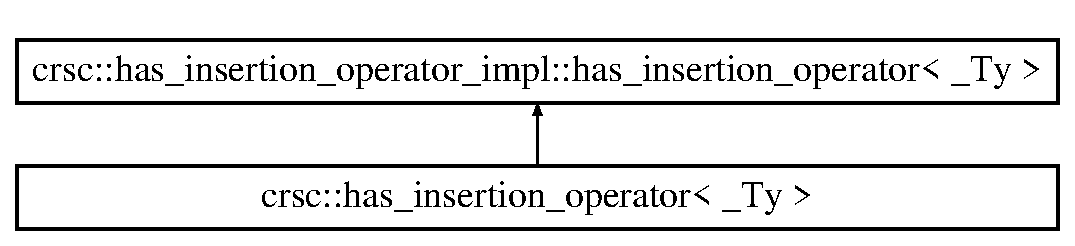
\includegraphics[height=2.000000cm]{structcrsc_1_1has__insertion__operator__impl_1_1has__insertion__operator}
\end{center}
\end{figure}
\subsection*{Static Public Attributes}
\begin{DoxyCompactItemize}
\item 
static std\+::ostream \& \hyperlink{structcrsc_1_1has__insertion__operator__impl_1_1has__insertion__operator_a99b73f462e0865446ba1ee620f4ddf5f}{os}
\item 
static const \+\_\+\+Ty \& \hyperlink{structcrsc_1_1has__insertion__operator__impl_1_1has__insertion__operator_ae450042bbfde15944de60bdb394a5df0}{t}
\item 
static const bool \hyperlink{structcrsc_1_1has__insertion__operator__impl_1_1has__insertion__operator_ab2d5f0eebe065054f52d71d070aede53}{value} = sizeof(\hyperlink{namespacecrsc_1_1has__insertion__operator__impl_aa24ee37999d6977adf54ba500c212841}{test}(\hyperlink{structcrsc_1_1has__insertion__operator__impl_1_1has__insertion__operator_a99b73f462e0865446ba1ee620f4ddf5f}{os} $<$$<$ \hyperlink{structcrsc_1_1has__insertion__operator__impl_1_1has__insertion__operator_ae450042bbfde15944de60bdb394a5df0}{t})) == sizeof(\hyperlink{namespacecrsc_1_1has__insertion__operator__impl_ab0dc7f56fe45b46b87bb577b7171858c}{yes})
\end{DoxyCompactItemize}


\subsection{Member Data Documentation}
\index{crsc\+::has\+\_\+insertion\+\_\+operator\+\_\+impl\+::has\+\_\+insertion\+\_\+operator@{crsc\+::has\+\_\+insertion\+\_\+operator\+\_\+impl\+::has\+\_\+insertion\+\_\+operator}!os@{os}}
\index{os@{os}!crsc\+::has\+\_\+insertion\+\_\+operator\+\_\+impl\+::has\+\_\+insertion\+\_\+operator@{crsc\+::has\+\_\+insertion\+\_\+operator\+\_\+impl\+::has\+\_\+insertion\+\_\+operator}}
\subsubsection[{\texorpdfstring{os}{os}}]{\setlength{\rightskip}{0pt plus 5cm}template$<$typename \+\_\+\+Ty $>$ std\+::ostream\& {\bf crsc\+::has\+\_\+insertion\+\_\+operator\+\_\+impl\+::has\+\_\+insertion\+\_\+operator}$<$ \+\_\+\+Ty $>$\+::os\hspace{0.3cm}{\ttfamily [static]}}\hypertarget{structcrsc_1_1has__insertion__operator__impl_1_1has__insertion__operator_a99b73f462e0865446ba1ee620f4ddf5f}{}\label{structcrsc_1_1has__insertion__operator__impl_1_1has__insertion__operator_a99b73f462e0865446ba1ee620f4ddf5f}
\index{crsc\+::has\+\_\+insertion\+\_\+operator\+\_\+impl\+::has\+\_\+insertion\+\_\+operator@{crsc\+::has\+\_\+insertion\+\_\+operator\+\_\+impl\+::has\+\_\+insertion\+\_\+operator}!t@{t}}
\index{t@{t}!crsc\+::has\+\_\+insertion\+\_\+operator\+\_\+impl\+::has\+\_\+insertion\+\_\+operator@{crsc\+::has\+\_\+insertion\+\_\+operator\+\_\+impl\+::has\+\_\+insertion\+\_\+operator}}
\subsubsection[{\texorpdfstring{t}{t}}]{\setlength{\rightskip}{0pt plus 5cm}template$<$typename \+\_\+\+Ty $>$ const \+\_\+\+Ty\& {\bf crsc\+::has\+\_\+insertion\+\_\+operator\+\_\+impl\+::has\+\_\+insertion\+\_\+operator}$<$ \+\_\+\+Ty $>$\+::t\hspace{0.3cm}{\ttfamily [static]}}\hypertarget{structcrsc_1_1has__insertion__operator__impl_1_1has__insertion__operator_ae450042bbfde15944de60bdb394a5df0}{}\label{structcrsc_1_1has__insertion__operator__impl_1_1has__insertion__operator_ae450042bbfde15944de60bdb394a5df0}
\index{crsc\+::has\+\_\+insertion\+\_\+operator\+\_\+impl\+::has\+\_\+insertion\+\_\+operator@{crsc\+::has\+\_\+insertion\+\_\+operator\+\_\+impl\+::has\+\_\+insertion\+\_\+operator}!value@{value}}
\index{value@{value}!crsc\+::has\+\_\+insertion\+\_\+operator\+\_\+impl\+::has\+\_\+insertion\+\_\+operator@{crsc\+::has\+\_\+insertion\+\_\+operator\+\_\+impl\+::has\+\_\+insertion\+\_\+operator}}
\subsubsection[{\texorpdfstring{value}{value}}]{\setlength{\rightskip}{0pt plus 5cm}template$<$typename \+\_\+\+Ty $>$ const bool {\bf crsc\+::has\+\_\+insertion\+\_\+operator\+\_\+impl\+::has\+\_\+insertion\+\_\+operator}$<$ \+\_\+\+Ty $>$\+::value = sizeof({\bf test}({\bf os} $<$$<$ {\bf t})) == sizeof({\bf yes})\hspace{0.3cm}{\ttfamily [static]}}\hypertarget{structcrsc_1_1has__insertion__operator__impl_1_1has__insertion__operator_ab2d5f0eebe065054f52d71d070aede53}{}\label{structcrsc_1_1has__insertion__operator__impl_1_1has__insertion__operator_ab2d5f0eebe065054f52d71d070aede53}


The documentation for this struct was generated from the following file\+:\begin{DoxyCompactItemize}
\item 
\hyperlink{dynamic__matrix_8h}{dynamic\+\_\+matrix.\+h}\end{DoxyCompactItemize}

\hypertarget{structcrsc_1_1has__insertion__operator}{}\section{crsc\+:\+:has\+\_\+insertion\+\_\+operator$<$ \+\_\+\+Ty $>$ Struct Template Reference}
\label{structcrsc_1_1has__insertion__operator}\index{crsc\+::has\+\_\+insertion\+\_\+operator$<$ \+\_\+\+Ty $>$@{crsc\+::has\+\_\+insertion\+\_\+operator$<$ \+\_\+\+Ty $>$}}


{\ttfamily \#include $<$dynamic\+\_\+matrix.\+h$>$}

Inheritance diagram for crsc\+:\+:has\+\_\+insertion\+\_\+operator$<$ \+\_\+\+Ty $>$\+:\begin{figure}[H]
\begin{center}
\leavevmode
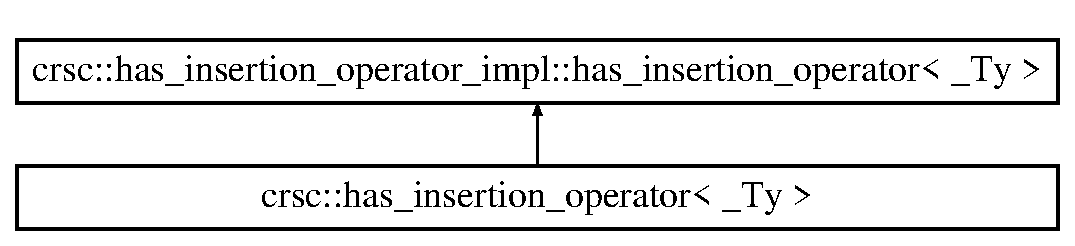
\includegraphics[height=2.000000cm]{structcrsc_1_1has__insertion__operator}
\end{center}
\end{figure}
\subsection*{Additional Inherited Members}


The documentation for this struct was generated from the following file\+:\begin{DoxyCompactItemize}
\item 
\hyperlink{dynamic__matrix_8h}{dynamic\+\_\+matrix.\+h}\end{DoxyCompactItemize}

\hypertarget{classcrsc_1_1priority__queue}{}\section{crsc\+:\+:priority\+\_\+queue$<$ \+\_\+\+Ty, \+\_\+\+Pr $>$ Class Template Reference}
\label{classcrsc_1_1priority__queue}\index{crsc\+::priority\+\_\+queue$<$ \+\_\+\+Ty, \+\_\+\+Pr $>$@{crsc\+::priority\+\_\+queue$<$ \+\_\+\+Ty, \+\_\+\+Pr $>$}}


A container adaptor (wrapping a {\ttfamily std\+::vector} as the heap storage) that provides constant time lookup of the largest (by default) element, at the expense of logarithmic insertion and extraction.  




{\ttfamily \#include $<$priority\+\_\+queue.\+h$>$}

\subsection*{Public Types}
\begin{DoxyCompactItemize}
\item 
typedef \+\_\+\+Ty \hyperlink{classcrsc_1_1priority__queue_a2a7d77c9465b6c918f67021e6eb926d7}{value\+\_\+type}
\item 
typedef \+\_\+\+Ty \& \hyperlink{classcrsc_1_1priority__queue_a2e667696d4a803d1a273fbd838cd6745}{reference}
\item 
typedef const \+\_\+\+Ty \& \hyperlink{classcrsc_1_1priority__queue_a654551a6a31b69c37ee6bac13b22d262}{const\+\_\+reference}
\item 
typedef \+\_\+\+Ty $\ast$ \hyperlink{classcrsc_1_1priority__queue_a6e6c3d342ac5217f91a33f480f626af5}{pointer}
\item 
typedef const \+\_\+\+Ty $\ast$ \hyperlink{classcrsc_1_1priority__queue_aeeaf3b92bbdb4475f0262588875e74b4}{const\+\_\+pointer}
\item 
typedef std\+::size\+\_\+t \hyperlink{classcrsc_1_1priority__queue_a2b1c9a55084026111d70a4fe869e0fbe}{size\+\_\+type}
\item 
typedef std\+::ptrdiff\+\_\+t \hyperlink{classcrsc_1_1priority__queue_a859155ca3fdb5d55d136bf6758630a39}{difference\+\_\+type}
\item 
typedef std\+::vector$<$ \+\_\+\+Ty $>$\+::\hyperlink{classcrsc_1_1priority__queue_a35736d93262db4fdd6d4a71bf785f9b9}{const\+\_\+iterator} \hyperlink{classcrsc_1_1priority__queue_a35736d93262db4fdd6d4a71bf785f9b9}{const\+\_\+iterator}
\item 
typedef std\+::vector$<$ \+\_\+\+Ty $>$\+::\hyperlink{classcrsc_1_1priority__queue_a8f8f07cb4cbb172b421ff41867fbcfb9}{const\+\_\+reverse\+\_\+iterator} \hyperlink{classcrsc_1_1priority__queue_a8f8f07cb4cbb172b421ff41867fbcfb9}{const\+\_\+reverse\+\_\+iterator}
\end{DoxyCompactItemize}
\subsection*{Public Member Functions}
\begin{DoxyCompactItemize}
\item 
\hyperlink{classcrsc_1_1priority__queue_ab8754476b3d20f14d8ede97e9d399088}{priority\+\_\+queue} (const \+\_\+\+Pr \&compare=\+\_\+\+Pr())
\begin{DoxyCompactList}\small\item\em Default constructor, initialises empty container with optional comparator argument. \end{DoxyCompactList}\item 
\hyperlink{classcrsc_1_1priority__queue_a64f1b37fd1bb0e580bc60b6770b75cc9}{priority\+\_\+queue} (const std\+::vector$<$ \hyperlink{classcrsc_1_1priority__queue_a2a7d77c9465b6c918f67021e6eb926d7}{value\+\_\+type} $>$ \&\+\_\+vec, const \+\_\+\+Pr \&compare=\+\_\+\+Pr())
\begin{DoxyCompactList}\small\item\em Constructs the container with contents of {\ttfamily \+\_\+vec}. \end{DoxyCompactList}\item 
\hyperlink{classcrsc_1_1priority__queue_a2cb52360d09b98e81e1a13f70d522745}{priority\+\_\+queue} (std\+::vector$<$ \hyperlink{classcrsc_1_1priority__queue_a2a7d77c9465b6c918f67021e6eb926d7}{value\+\_\+type} $>$ \&\&\+\_\+vec, const \+\_\+\+Pr \&compare=\+\_\+\+Pr())
\begin{DoxyCompactList}\small\item\em Constructs the container with contents of {\ttfamily \+\_\+vec} using move-\/semantics. \end{DoxyCompactList}\item 
{\footnotesize template$<$class Input\+It $>$ }\\\hyperlink{classcrsc_1_1priority__queue_a702c30cd7302fc7cd7ba83e5a3f6361e}{priority\+\_\+queue} (Input\+It first, Input\+It last, const \+\_\+\+Pr \&compare=\+\_\+\+Pr())
\begin{DoxyCompactList}\small\item\em Constructs the container with the contents of the range {\ttfamily \mbox{[}first, last)}. \end{DoxyCompactList}\item 
\hyperlink{classcrsc_1_1priority__queue_a42a9483593902a7319bda777c5f68098}{priority\+\_\+queue} (const \hyperlink{classcrsc_1_1priority__queue}{priority\+\_\+queue} \&\+\_\+other) noexcept
\begin{DoxyCompactList}\small\item\em Constructs the container with a copy of the contents of {\ttfamily \+\_\+other}. \end{DoxyCompactList}\item 
\hyperlink{classcrsc_1_1priority__queue_abcb59ed0013620d12e7b5d737df76529}{priority\+\_\+queue} (\hyperlink{classcrsc_1_1priority__queue}{priority\+\_\+queue} \&\&\+\_\+other) noexcept
\begin{DoxyCompactList}\small\item\em Constructs the container with the contents of {\ttfamily \+\_\+other} using move-\/semantics. \end{DoxyCompactList}\item 
\hyperlink{classcrsc_1_1priority__queue_a83a4b61c8ce19b7690e8d9b7828cc9c2}{$\sim$priority\+\_\+queue} ()
\begin{DoxyCompactList}\small\item\em Destructs the container. The destructors of the elements are called used storage is deallocated. \end{DoxyCompactList}\item 
\hyperlink{classcrsc_1_1priority__queue}{priority\+\_\+queue} \& \hyperlink{classcrsc_1_1priority__queue_aa514b407798f48c5f5f2cd21256997a7}{operator=} (const \hyperlink{classcrsc_1_1priority__queue}{priority\+\_\+queue} \&\+\_\+other)
\begin{DoxyCompactList}\small\item\em Copy-\/assignment operator, replaces the contents of the container with the a copy of the contents of {\ttfamily \+\_\+other}. \end{DoxyCompactList}\item 
\hyperlink{classcrsc_1_1priority__queue}{priority\+\_\+queue} \& \hyperlink{classcrsc_1_1priority__queue_a7a9bc10de10f479718c05a1f6df55cf1}{operator=} (\hyperlink{classcrsc_1_1priority__queue}{priority\+\_\+queue} \&\&\+\_\+other)
\begin{DoxyCompactList}\small\item\em Move-\/assignment operator, replaces the contents of the container with the contents of {\ttfamily \+\_\+other} using move-\/semantics. \end{DoxyCompactList}\item 
bool \hyperlink{classcrsc_1_1priority__queue_acc3ad538699e923b4ee50bd30c6379f6}{empty} () const  noexcept
\begin{DoxyCompactList}\small\item\em Checks whether the container is empty. \end{DoxyCompactList}\item 
\hyperlink{classcrsc_1_1priority__queue_a2b1c9a55084026111d70a4fe869e0fbe}{size\+\_\+type} \hyperlink{classcrsc_1_1priority__queue_af2e208f5e6d7de9bce98ab6f225107aa}{size} () const  noexcept
\begin{DoxyCompactList}\small\item\em Returns the number of elements in the container. \end{DoxyCompactList}\item 
\hyperlink{classcrsc_1_1priority__queue_a2b1c9a55084026111d70a4fe869e0fbe}{size\+\_\+type} \hyperlink{classcrsc_1_1priority__queue_a38a462a9b04c8bd8e96deed40e8022f8}{max\+\_\+size} () const  noexcept
\begin{DoxyCompactList}\small\item\em Returns the maximum number of elements the container is able to hold due to system or library implementation limitations. \end{DoxyCompactList}\item 
\hyperlink{classcrsc_1_1priority__queue_a654551a6a31b69c37ee6bac13b22d262}{const\+\_\+reference} \hyperlink{classcrsc_1_1priority__queue_a69fa407b73905801ebceb4b857484247}{top} () const 
\begin{DoxyCompactList}\small\item\em Accesses the top element of the container without popping it. \end{DoxyCompactList}\item 
\hyperlink{classcrsc_1_1priority__queue_a35736d93262db4fdd6d4a71bf785f9b9}{const\+\_\+iterator} \hyperlink{classcrsc_1_1priority__queue_af2ca2cc288875dd4fda147260055b81d}{find} (const \hyperlink{classcrsc_1_1priority__queue_a2a7d77c9465b6c918f67021e6eb926d7}{value\+\_\+type} \&\+\_\+val) const 
\begin{DoxyCompactList}\small\item\em Finds the first instance of an element in the container. \end{DoxyCompactList}\item 
std\+::vector$<$ \hyperlink{classcrsc_1_1priority__queue_a35736d93262db4fdd6d4a71bf785f9b9}{const\+\_\+iterator} $>$ \hyperlink{classcrsc_1_1priority__queue_ae0d4ae80ad39510a1b70e8dcdccf6aaa}{find\+\_\+all} (const \hyperlink{classcrsc_1_1priority__queue_a2a7d77c9465b6c918f67021e6eb926d7}{value\+\_\+type} \&\+\_\+val) const 
\begin{DoxyCompactList}\small\item\em Finds all instances of an element in the container. \end{DoxyCompactList}\item 
{\footnotesize template$<$class Unary\+Predicate $>$ }\\\hyperlink{classcrsc_1_1priority__queue_a35736d93262db4fdd6d4a71bf785f9b9}{const\+\_\+iterator} \hyperlink{classcrsc_1_1priority__queue_a21f89662e99dc2f3d2d226bb7973496e}{find} (Unary\+Predicate \+\_\+p) const 
\begin{DoxyCompactList}\small\item\em Find the first instance of an element in the container based on a unary predicate. \end{DoxyCompactList}\item 
{\footnotesize template$<$class Unary\+Predicate $>$ }\\std\+::vector$<$ \hyperlink{classcrsc_1_1priority__queue_a35736d93262db4fdd6d4a71bf785f9b9}{const\+\_\+iterator} $>$ \hyperlink{classcrsc_1_1priority__queue_ad759259910ae44d561c6575f3af8d82c}{find\+\_\+all} (Unary\+Predicate \+\_\+p) const 
\begin{DoxyCompactList}\small\item\em Finds all instances of an element in the container based on a unary predicate. \end{DoxyCompactList}\item 
{\footnotesize template$<$class \+\_\+\+Uty  = \+\_\+\+Ty, class  = std\+::enable\+\_\+if\+\_\+t$<$std\+::is\+\_\+copy\+\_\+assignable$<$\+\_\+\+Uty$>$\+::value$>$$>$ }\\std\+::ostream \& \hyperlink{classcrsc_1_1priority__queue_adef837b2da436690c8a1e2214c47bac9}{write\+\_\+ordered} (std\+::ostream \&\+\_\+os, char \+\_\+delim= \textquotesingle{} \textquotesingle{}) const  noexcept
\begin{DoxyCompactList}\small\item\em Writes the contents of the container to a {\ttfamily std\+::ostream} in heap-\/order. \end{DoxyCompactList}\item 
std\+::ostream \& \hyperlink{classcrsc_1_1priority__queue_ac279b3a3936989a66c9d65fa922edcab}{write} (std\+::ostream \&\+\_\+os, char \+\_\+delim= \textquotesingle{} \textquotesingle{}) const  noexcept
\begin{DoxyCompactList}\small\item\em Writes the contents of the container to a {\ttfamily std\+::ostream} in non-\/heap-\/order, the elements shall be written in the order that they are stored in the underlying contiguous memory block. \end{DoxyCompactList}\item 
{\footnotesize template$<$class \+\_\+\+Uty  = \+\_\+\+Ty, class  = std\+::enable\+\_\+if\+\_\+t$<$std\+::is\+\_\+copy\+\_\+assignable$<$\+\_\+\+Uty$>$\+::value$>$$>$ }\\void \hyperlink{classcrsc_1_1priority__queue_a9447e88a7c478c4b7a6b6b95f62cce6e}{enqueue} (const \hyperlink{classcrsc_1_1priority__queue_a2a7d77c9465b6c918f67021e6eb926d7}{value\+\_\+type} \&\+\_\+val)
\begin{DoxyCompactList}\small\item\em Pushes an item into the container and sorts it. \end{DoxyCompactList}\item 
{\footnotesize template$<$class \+\_\+\+Uty  = \+\_\+\+Ty, class  = std\+::enable\+\_\+if\+\_\+t$<$std\+::is\+\_\+move\+\_\+assignable$<$\+\_\+\+Uty$>$\+::value$>$$>$ }\\void \hyperlink{classcrsc_1_1priority__queue_a7104c88c185858be0b31e8219c77115e}{enqueue} (\hyperlink{classcrsc_1_1priority__queue_a2a7d77c9465b6c918f67021e6eb926d7}{value\+\_\+type} \&\&\+\_\+val)
\begin{DoxyCompactList}\small\item\em Pushes an item into the container via move-\/insertion and sorts it. \end{DoxyCompactList}\item 
{\footnotesize template$<$class... Args$>$ }\\void \hyperlink{classcrsc_1_1priority__queue_a6152229fef8983341ee6eda345a39cc7}{emplace} (Args \&\&...\+\_\+args)
\begin{DoxyCompactList}\small\item\em Constructs element in-\/place and sorts the underlying container. \end{DoxyCompactList}\item 
void \hyperlink{classcrsc_1_1priority__queue_a0b1fec17785494ed66d9f85c2079d1e7}{dequeue} () noexcept
\begin{DoxyCompactList}\small\item\em Pops the top item from the container. \end{DoxyCompactList}\item 
void \hyperlink{classcrsc_1_1priority__queue_a6d9196a9adcadc5f0c4e6e8e5559f4d7}{clear} () noexcept
\begin{DoxyCompactList}\small\item\em Clears all items from the container. \end{DoxyCompactList}\item 
{\footnotesize template$<$class \+\_\+\+Uty  = \+\_\+\+Ty, class  = std\+::enable\+\_\+if\+\_\+t$<$std\+::is\+\_\+copy\+\_\+assignable$<$\+\_\+\+Uty$>$\+::value$>$$>$ }\\void \hyperlink{classcrsc_1_1priority__queue_a77fc76e3682abf042bfbdfcce78b41aa}{alter} (const \hyperlink{classcrsc_1_1priority__queue_a2a7d77c9465b6c918f67021e6eb926d7}{value\+\_\+type} \&\+\_\+val\+\_\+find, const \hyperlink{classcrsc_1_1priority__queue_a2a7d77c9465b6c918f67021e6eb926d7}{value\+\_\+type} \&\+\_\+alter\+\_\+to\+\_\+val)
\begin{DoxyCompactList}\small\item\em Alters the first instance of the specified value {\ttfamily \+\_\+val\+\_\+find} in the container to {\ttfamily \+\_\+alter\+\_\+to\+\_\+val} by copy-\/assignment. If {\ttfamily \+\_\+val\+\_\+find} does not exist in the container, this method does nothing. \end{DoxyCompactList}\item 
{\footnotesize template$<$class Unary\+Predicate , class \+\_\+\+Uty  = \+\_\+\+Ty, class  = std\+::enable\+\_\+if\+\_\+t$<$std\+::is\+\_\+copy\+\_\+assignable$<$\+\_\+\+Uty$>$\+::value$>$$>$ }\\void \hyperlink{classcrsc_1_1priority__queue_abe2ae7e923d7bfd53dd79c15d4c4fd26}{alter} (const \hyperlink{classcrsc_1_1priority__queue_a2a7d77c9465b6c918f67021e6eb926d7}{value\+\_\+type} \&\+\_\+alter\+\_\+to\+\_\+val, Unary\+Predicate \+\_\+p)
\begin{DoxyCompactList}\small\item\em Alters the first instance of an item in the container for which the unary predicate {\ttfamily \+\_\+p} is satisfied to {\ttfamily \+\_\+alter\+\_\+to\+\_\+val} by copy-\/assignment. If there are no such items in the container which satisfy {\ttfamily \+\_\+p} then this method does nothing. \end{DoxyCompactList}\item 
{\footnotesize template$<$class Unary\+Predicate , class \+\_\+\+Uty  = \+\_\+\+Ty, class  = std\+::enable\+\_\+if\+\_\+t$<$std\+::is\+\_\+move\+\_\+assignable$<$\+\_\+\+Uty$>$\+::value$>$$>$ }\\void \hyperlink{classcrsc_1_1priority__queue_a87fbb620ca34e1d02480f471717acd40}{alter} (\hyperlink{classcrsc_1_1priority__queue_a2a7d77c9465b6c918f67021e6eb926d7}{value\+\_\+type} \&\&\+\_\+alter\+\_\+to\+\_\+val, Unary\+Predicate \+\_\+p)
\begin{DoxyCompactList}\small\item\em Alters the first instance of an item in the container for which the unary predicate {\ttfamily \+\_\+p} is satisfifed to {\ttfamily \+\_\+alter\+\_\+to\+\_\+val} by move-\/assignment. If there are no such items in the container which satisfy {\ttfamily \+\_\+p} then this method does nothing. \end{DoxyCompactList}\item 
void \hyperlink{classcrsc_1_1priority__queue_a97d76087502f3213ee56ff2391a11111}{alter\+\_\+all} (const \hyperlink{classcrsc_1_1priority__queue_a2a7d77c9465b6c918f67021e6eb926d7}{value\+\_\+type} \&\+\_\+val\+\_\+find, const \hyperlink{classcrsc_1_1priority__queue_a2a7d77c9465b6c918f67021e6eb926d7}{value\+\_\+type} \&\+\_\+alter\+\_\+to\+\_\+val)
\begin{DoxyCompactList}\small\item\em Alters all instances of the specified value {\ttfamily \+\_\+val\+\_\+find} in the container to {\ttfamily \+\_\+alter\+\_\+to\+\_\+val} by copy-\/assignment. If {\ttfamily \+\_\+val\+\_\+find} does not exist in the container, this method does nothing. \end{DoxyCompactList}\item 
{\footnotesize template$<$class Unary\+Predicate $>$ }\\void \hyperlink{classcrsc_1_1priority__queue_ac9ee338a0ae1a1f96c37ffed5664a8e0}{alter\+\_\+all} (const \hyperlink{classcrsc_1_1priority__queue_a2a7d77c9465b6c918f67021e6eb926d7}{value\+\_\+type} \&\+\_\+alter\+\_\+to\+\_\+val, Unary\+Predicate \+\_\+p)
\begin{DoxyCompactList}\small\item\em Alters all instances of items in the container for which the unary predicate {\ttfamily \+\_\+p} is satisifed to {\ttfamily \+\_\+alter\+\_\+to\+\_\+val} by copy-\/assignment. If there are no such items in the container which satisfy {\ttfamily \+\_\+p} then this method does nothing. \end{DoxyCompactList}\item 
void \hyperlink{classcrsc_1_1priority__queue_acaf2818cb6bb65a84806fe5e0253a5c5}{swap} (\hyperlink{classcrsc_1_1priority__queue}{priority\+\_\+queue} \&\+\_\+other)
\begin{DoxyCompactList}\small\item\em Exchanges the contents of the container with those of {\ttfamily \+\_\+other}. Does not cause references and iterators to associate with the other container. \end{DoxyCompactList}\item 
\hyperlink{classcrsc_1_1priority__queue_a35736d93262db4fdd6d4a71bf785f9b9}{const\+\_\+iterator} \hyperlink{classcrsc_1_1priority__queue_aee3d3ed7f8581669cfd890333b349fc6}{cbegin} () const  noexcept
\begin{DoxyCompactList}\small\item\em Returns a const\+\_\+iterator the first element of the container. \end{DoxyCompactList}\item 
\hyperlink{classcrsc_1_1priority__queue_a35736d93262db4fdd6d4a71bf785f9b9}{const\+\_\+iterator} \hyperlink{classcrsc_1_1priority__queue_a34e337055fa734f662ff5fae137cbefb}{cend} () const  noexcept
\begin{DoxyCompactList}\small\item\em Returns a const\+\_\+iterator to the past-\/the-\/end element of the container. \end{DoxyCompactList}\item 
\hyperlink{classcrsc_1_1priority__queue_a8f8f07cb4cbb172b421ff41867fbcfb9}{const\+\_\+reverse\+\_\+iterator} \hyperlink{classcrsc_1_1priority__queue_a0c0992bca6797f683543ba15cceeebad}{crbegin} () const  noexcept
\begin{DoxyCompactList}\small\item\em Returns a const\+\_\+reverse\+\_\+iterator to the first element of the reversed container. It corresponds to the last element of the non-\/reversed container. \end{DoxyCompactList}\item 
\hyperlink{classcrsc_1_1priority__queue_a8f8f07cb4cbb172b421ff41867fbcfb9}{const\+\_\+reverse\+\_\+iterator} \hyperlink{classcrsc_1_1priority__queue_a82953a7117eaabd34c66f62a4d664dfd}{crend} () const  noexcept
\begin{DoxyCompactList}\small\item\em Returns a const\+\_\+reverse\+\_\+iterator to the past-\/the-\/end element of the reversed container. It corresponds to the element preceding the first element of the non-\/reversed container. \end{DoxyCompactList}\end{DoxyCompactItemize}
\subsection*{Private Member Functions}
\begin{DoxyCompactItemize}
\item 
void \hyperlink{classcrsc_1_1priority__queue_a0eeef0c2e3ac88be9f9e5f77ec7b71cc}{bubble\+\_\+down} (\hyperlink{classcrsc_1_1priority__queue_a2b1c9a55084026111d70a4fe869e0fbe}{size\+\_\+type} \+\_\+pos)
\begin{DoxyCompactList}\small\item\em Bubbles down the heap from a given vector index, performing swaps based on comparator conditions. \end{DoxyCompactList}\item 
void \hyperlink{classcrsc_1_1priority__queue_a39f493e04737a79c673cc29a94c165cc}{bubble\+\_\+up} (\hyperlink{classcrsc_1_1priority__queue_a2b1c9a55084026111d70a4fe869e0fbe}{size\+\_\+type} \+\_\+pos)
\begin{DoxyCompactList}\small\item\em Bubbles up the heap from a given vector index, performing swaps based on comparator conditions. \end{DoxyCompactList}\item 
void \hyperlink{classcrsc_1_1priority__queue_ad4793f4fd1e74671fd147a1aa0308933}{pop\+\_\+top} () noexcept
\begin{DoxyCompactList}\small\item\em Removes the top item from the heap and bubbles down from new top. \end{DoxyCompactList}\item 
void \hyperlink{classcrsc_1_1priority__queue_a0ff3f63750679149c557ac30f8775a96}{heapify} () noexcept
\begin{DoxyCompactList}\small\item\em Performs heapification of entire binary heap, bubbling down from each index such that binary heap invariant is guaranteed. \end{DoxyCompactList}\end{DoxyCompactItemize}
\subsection*{Private Attributes}
\begin{DoxyCompactItemize}
\item 
std\+::vector$<$ \hyperlink{classcrsc_1_1priority__queue_a2a7d77c9465b6c918f67021e6eb926d7}{value\+\_\+type} $>$ \hyperlink{classcrsc_1_1priority__queue_ab21e7fd1647424d3580e86dc0aec2597}{heap\+\_\+vec}
\item 
\+\_\+\+Pr \hyperlink{classcrsc_1_1priority__queue_aeb39fce3f1ec0299540cf5431ca4129e}{comp}
\end{DoxyCompactItemize}


\subsection{Detailed Description}
\subsubsection*{template$<$typename \+\_\+\+Ty, class \+\_\+\+Pr = std\+::less$<$\+\_\+\+Ty$>$$>$\\*
class crsc\+::priority\+\_\+queue$<$ \+\_\+\+Ty, \+\_\+\+Pr $>$}

A container adaptor (wrapping a {\ttfamily std\+::vector} as the heap storage) that provides constant time lookup of the largest (by default) element, at the expense of logarithmic insertion and extraction. 

The element priorities are compared by default using {\ttfamily std\+::less$<$\+\_\+\+Ty$>$} such that the largest element is always at the top of the heap, this comparator can be altered as a template argument to any other {\ttfamily Compare} type such as {\ttfamily std\+::greater$<$\+\_\+\+Ty$>$} which would define minimum binary heap behaviour such that the smallest element is always on the top of the heap (providing constant lookup for the smallest item).

Unlike {\ttfamily std\+::priority\+\_\+queue} this container only allows the wrapping of a {\ttfamily std\+::vector} as the underlying heap container. However, this version of a priority queue provides methods to search for items in the container, alter item values, clear the container and iterate over the container with {\ttfamily const\+\_\+iterator}s which the S\+TL priority queue does not provide. In addition, similarly to {\ttfamily std\+::priority\+\_\+queue}, every method is guaranteed to preserve the class invariant such that the heap is not invalidated at any point between method calls.


\begin{DoxyTemplParams}{Template Parameters}
{\em \+\_\+\+Ty} & The type of the elements. \\
\hline
{\em \+\_\+\+Pr} & A {\ttfamily Compare} type providing a strict weak ordering, defaults to {\ttfamily std\+::less$<$\+\_\+\+Ty$>$}. \\
\hline
\end{DoxyTemplParams}
\begin{DoxyInvariant}{Invariant}
The heap (whose ordering/behaviour is defined by the comparator {\ttfamily \+\_\+\+Pr}) shall never be invalidated between method calls, and if any exceptions are thrown by a method the heap shall never be left in a state which would invalidate the heap. 
\end{DoxyInvariant}
\begin{DoxyAuthor}{Author}
Samuel Rowlinson 
\end{DoxyAuthor}
\begin{DoxyDate}{Date}
July, 2016 
\end{DoxyDate}


\subsection{Member Typedef Documentation}
\index{crsc\+::priority\+\_\+queue@{crsc\+::priority\+\_\+queue}!const\+\_\+iterator@{const\+\_\+iterator}}
\index{const\+\_\+iterator@{const\+\_\+iterator}!crsc\+::priority\+\_\+queue@{crsc\+::priority\+\_\+queue}}
\subsubsection[{\texorpdfstring{const\+\_\+iterator}{const_iterator}}]{\setlength{\rightskip}{0pt plus 5cm}template$<$typename \+\_\+\+Ty, class \+\_\+\+Pr = std\+::less$<$\+\_\+\+Ty$>$$>$ typedef std\+::vector$<$\+\_\+\+Ty$>$\+::{\bf const\+\_\+iterator} {\bf crsc\+::priority\+\_\+queue}$<$ \+\_\+\+Ty, \+\_\+\+Pr $>$\+::{\bf const\+\_\+iterator}}\hypertarget{classcrsc_1_1priority__queue_a35736d93262db4fdd6d4a71bf785f9b9}{}\label{classcrsc_1_1priority__queue_a35736d93262db4fdd6d4a71bf785f9b9}
\index{crsc\+::priority\+\_\+queue@{crsc\+::priority\+\_\+queue}!const\+\_\+pointer@{const\+\_\+pointer}}
\index{const\+\_\+pointer@{const\+\_\+pointer}!crsc\+::priority\+\_\+queue@{crsc\+::priority\+\_\+queue}}
\subsubsection[{\texorpdfstring{const\+\_\+pointer}{const_pointer}}]{\setlength{\rightskip}{0pt plus 5cm}template$<$typename \+\_\+\+Ty, class \+\_\+\+Pr = std\+::less$<$\+\_\+\+Ty$>$$>$ typedef const \+\_\+\+Ty$\ast$ {\bf crsc\+::priority\+\_\+queue}$<$ \+\_\+\+Ty, \+\_\+\+Pr $>$\+::{\bf const\+\_\+pointer}}\hypertarget{classcrsc_1_1priority__queue_aeeaf3b92bbdb4475f0262588875e74b4}{}\label{classcrsc_1_1priority__queue_aeeaf3b92bbdb4475f0262588875e74b4}
\index{crsc\+::priority\+\_\+queue@{crsc\+::priority\+\_\+queue}!const\+\_\+reference@{const\+\_\+reference}}
\index{const\+\_\+reference@{const\+\_\+reference}!crsc\+::priority\+\_\+queue@{crsc\+::priority\+\_\+queue}}
\subsubsection[{\texorpdfstring{const\+\_\+reference}{const_reference}}]{\setlength{\rightskip}{0pt plus 5cm}template$<$typename \+\_\+\+Ty, class \+\_\+\+Pr = std\+::less$<$\+\_\+\+Ty$>$$>$ typedef const \+\_\+\+Ty\& {\bf crsc\+::priority\+\_\+queue}$<$ \+\_\+\+Ty, \+\_\+\+Pr $>$\+::{\bf const\+\_\+reference}}\hypertarget{classcrsc_1_1priority__queue_a654551a6a31b69c37ee6bac13b22d262}{}\label{classcrsc_1_1priority__queue_a654551a6a31b69c37ee6bac13b22d262}
\index{crsc\+::priority\+\_\+queue@{crsc\+::priority\+\_\+queue}!const\+\_\+reverse\+\_\+iterator@{const\+\_\+reverse\+\_\+iterator}}
\index{const\+\_\+reverse\+\_\+iterator@{const\+\_\+reverse\+\_\+iterator}!crsc\+::priority\+\_\+queue@{crsc\+::priority\+\_\+queue}}
\subsubsection[{\texorpdfstring{const\+\_\+reverse\+\_\+iterator}{const_reverse_iterator}}]{\setlength{\rightskip}{0pt plus 5cm}template$<$typename \+\_\+\+Ty, class \+\_\+\+Pr = std\+::less$<$\+\_\+\+Ty$>$$>$ typedef std\+::vector$<$\+\_\+\+Ty$>$\+::{\bf const\+\_\+reverse\+\_\+iterator} {\bf crsc\+::priority\+\_\+queue}$<$ \+\_\+\+Ty, \+\_\+\+Pr $>$\+::{\bf const\+\_\+reverse\+\_\+iterator}}\hypertarget{classcrsc_1_1priority__queue_a8f8f07cb4cbb172b421ff41867fbcfb9}{}\label{classcrsc_1_1priority__queue_a8f8f07cb4cbb172b421ff41867fbcfb9}
\index{crsc\+::priority\+\_\+queue@{crsc\+::priority\+\_\+queue}!difference\+\_\+type@{difference\+\_\+type}}
\index{difference\+\_\+type@{difference\+\_\+type}!crsc\+::priority\+\_\+queue@{crsc\+::priority\+\_\+queue}}
\subsubsection[{\texorpdfstring{difference\+\_\+type}{difference_type}}]{\setlength{\rightskip}{0pt plus 5cm}template$<$typename \+\_\+\+Ty, class \+\_\+\+Pr = std\+::less$<$\+\_\+\+Ty$>$$>$ typedef std\+::ptrdiff\+\_\+t {\bf crsc\+::priority\+\_\+queue}$<$ \+\_\+\+Ty, \+\_\+\+Pr $>$\+::{\bf difference\+\_\+type}}\hypertarget{classcrsc_1_1priority__queue_a859155ca3fdb5d55d136bf6758630a39}{}\label{classcrsc_1_1priority__queue_a859155ca3fdb5d55d136bf6758630a39}
\index{crsc\+::priority\+\_\+queue@{crsc\+::priority\+\_\+queue}!pointer@{pointer}}
\index{pointer@{pointer}!crsc\+::priority\+\_\+queue@{crsc\+::priority\+\_\+queue}}
\subsubsection[{\texorpdfstring{pointer}{pointer}}]{\setlength{\rightskip}{0pt plus 5cm}template$<$typename \+\_\+\+Ty, class \+\_\+\+Pr = std\+::less$<$\+\_\+\+Ty$>$$>$ typedef \+\_\+\+Ty$\ast$ {\bf crsc\+::priority\+\_\+queue}$<$ \+\_\+\+Ty, \+\_\+\+Pr $>$\+::{\bf pointer}}\hypertarget{classcrsc_1_1priority__queue_a6e6c3d342ac5217f91a33f480f626af5}{}\label{classcrsc_1_1priority__queue_a6e6c3d342ac5217f91a33f480f626af5}
\index{crsc\+::priority\+\_\+queue@{crsc\+::priority\+\_\+queue}!reference@{reference}}
\index{reference@{reference}!crsc\+::priority\+\_\+queue@{crsc\+::priority\+\_\+queue}}
\subsubsection[{\texorpdfstring{reference}{reference}}]{\setlength{\rightskip}{0pt plus 5cm}template$<$typename \+\_\+\+Ty, class \+\_\+\+Pr = std\+::less$<$\+\_\+\+Ty$>$$>$ typedef \+\_\+\+Ty\& {\bf crsc\+::priority\+\_\+queue}$<$ \+\_\+\+Ty, \+\_\+\+Pr $>$\+::{\bf reference}}\hypertarget{classcrsc_1_1priority__queue_a2e667696d4a803d1a273fbd838cd6745}{}\label{classcrsc_1_1priority__queue_a2e667696d4a803d1a273fbd838cd6745}
\index{crsc\+::priority\+\_\+queue@{crsc\+::priority\+\_\+queue}!size\+\_\+type@{size\+\_\+type}}
\index{size\+\_\+type@{size\+\_\+type}!crsc\+::priority\+\_\+queue@{crsc\+::priority\+\_\+queue}}
\subsubsection[{\texorpdfstring{size\+\_\+type}{size_type}}]{\setlength{\rightskip}{0pt plus 5cm}template$<$typename \+\_\+\+Ty, class \+\_\+\+Pr = std\+::less$<$\+\_\+\+Ty$>$$>$ typedef std\+::size\+\_\+t {\bf crsc\+::priority\+\_\+queue}$<$ \+\_\+\+Ty, \+\_\+\+Pr $>$\+::{\bf size\+\_\+type}}\hypertarget{classcrsc_1_1priority__queue_a2b1c9a55084026111d70a4fe869e0fbe}{}\label{classcrsc_1_1priority__queue_a2b1c9a55084026111d70a4fe869e0fbe}
\index{crsc\+::priority\+\_\+queue@{crsc\+::priority\+\_\+queue}!value\+\_\+type@{value\+\_\+type}}
\index{value\+\_\+type@{value\+\_\+type}!crsc\+::priority\+\_\+queue@{crsc\+::priority\+\_\+queue}}
\subsubsection[{\texorpdfstring{value\+\_\+type}{value_type}}]{\setlength{\rightskip}{0pt plus 5cm}template$<$typename \+\_\+\+Ty, class \+\_\+\+Pr = std\+::less$<$\+\_\+\+Ty$>$$>$ typedef \+\_\+\+Ty {\bf crsc\+::priority\+\_\+queue}$<$ \+\_\+\+Ty, \+\_\+\+Pr $>$\+::{\bf value\+\_\+type}}\hypertarget{classcrsc_1_1priority__queue_a2a7d77c9465b6c918f67021e6eb926d7}{}\label{classcrsc_1_1priority__queue_a2a7d77c9465b6c918f67021e6eb926d7}


\subsection{Constructor \& Destructor Documentation}
\index{crsc\+::priority\+\_\+queue@{crsc\+::priority\+\_\+queue}!priority\+\_\+queue@{priority\+\_\+queue}}
\index{priority\+\_\+queue@{priority\+\_\+queue}!crsc\+::priority\+\_\+queue@{crsc\+::priority\+\_\+queue}}
\subsubsection[{\texorpdfstring{priority\+\_\+queue(const \+\_\+\+Pr \&compare=\+\_\+\+Pr())}{priority_queue(const _Pr &compare=_Pr())}}]{\setlength{\rightskip}{0pt plus 5cm}template$<$typename \+\_\+\+Ty, class \+\_\+\+Pr = std\+::less$<$\+\_\+\+Ty$>$$>$ {\bf crsc\+::priority\+\_\+queue}$<$ \+\_\+\+Ty, \+\_\+\+Pr $>$\+::{\bf priority\+\_\+queue} (
\begin{DoxyParamCaption}
\item[{const \+\_\+\+Pr \&}]{compare = {\ttfamily \+\_\+Pr()}}
\end{DoxyParamCaption}
)\hspace{0.3cm}{\ttfamily [inline]}, {\ttfamily [explicit]}}\hypertarget{classcrsc_1_1priority__queue_ab8754476b3d20f14d8ede97e9d399088}{}\label{classcrsc_1_1priority__queue_ab8754476b3d20f14d8ede97e9d399088}


Default constructor, initialises empty container with optional comparator argument. 


\begin{DoxyParams}{Parameters}
{\em compare} & Comparator function object to initialise underlying comparison functor. \\
\hline
\end{DoxyParams}
\begin{DoxyParagraph}{Complexity}
Complexity of construction of {\ttfamily compare} (typically constant). 
\end{DoxyParagraph}
\begin{DoxyParagraph}{Exception Safety}
No-\/throw guarantee if {\ttfamily \+\_\+\+Pr()} does not throw, otherwise dependent upon exception safety of {\ttfamily compare}. 
\end{DoxyParagraph}
\index{crsc\+::priority\+\_\+queue@{crsc\+::priority\+\_\+queue}!priority\+\_\+queue@{priority\+\_\+queue}}
\index{priority\+\_\+queue@{priority\+\_\+queue}!crsc\+::priority\+\_\+queue@{crsc\+::priority\+\_\+queue}}
\subsubsection[{\texorpdfstring{priority\+\_\+queue(const std\+::vector$<$ value\+\_\+type $>$ \&\+\_\+vec, const \+\_\+\+Pr \&compare=\+\_\+\+Pr())}{priority_queue(const std::vector< value_type > &_vec, const _Pr &compare=_Pr())}}]{\setlength{\rightskip}{0pt plus 5cm}template$<$typename \+\_\+\+Ty, class \+\_\+\+Pr = std\+::less$<$\+\_\+\+Ty$>$$>$ {\bf crsc\+::priority\+\_\+queue}$<$ \+\_\+\+Ty, \+\_\+\+Pr $>$\+::{\bf priority\+\_\+queue} (
\begin{DoxyParamCaption}
\item[{const std\+::vector$<$ {\bf value\+\_\+type} $>$ \&}]{\+\_\+vec, }
\item[{const \+\_\+\+Pr \&}]{compare = {\ttfamily \+\_\+Pr()}}
\end{DoxyParamCaption}
)\hspace{0.3cm}{\ttfamily [inline]}, {\ttfamily [explicit]}}\hypertarget{classcrsc_1_1priority__queue_a64f1b37fd1bb0e580bc60b6770b75cc9}{}\label{classcrsc_1_1priority__queue_a64f1b37fd1bb0e580bc60b6770b75cc9}


Constructs the container with contents of {\ttfamily \+\_\+vec}. 


\begin{DoxyParams}{Parameters}
{\em \+\_\+vec} & Container to initialise contents with. \\
\hline
{\em compare} & Comparator function object to initialise underlying comparison functor. \\
\hline
\end{DoxyParams}
\begin{DoxyParagraph}{Complexity}
Linear in {\ttfamily \+\_\+vec.\+size()} multiplied by logarithmic in {\ttfamily \+\_\+vec.\+size()} plus an additional linear in {\ttfamily \+\_\+vec.\+size()} for vector copy. 
\end{DoxyParagraph}
\begin{DoxyParagraph}{Exception Safety}
No-\/throw guarantee if {\ttfamily \+\_\+\+Pr()} does not throw, otherwise dependent upon exception safety of {\ttfamily compare}. 
\end{DoxyParagraph}
\index{crsc\+::priority\+\_\+queue@{crsc\+::priority\+\_\+queue}!priority\+\_\+queue@{priority\+\_\+queue}}
\index{priority\+\_\+queue@{priority\+\_\+queue}!crsc\+::priority\+\_\+queue@{crsc\+::priority\+\_\+queue}}
\subsubsection[{\texorpdfstring{priority\+\_\+queue(std\+::vector$<$ value\+\_\+type $>$ \&\&\+\_\+vec, const \+\_\+\+Pr \&compare=\+\_\+\+Pr())}{priority_queue(std::vector< value_type > &&_vec, const _Pr &compare=_Pr())}}]{\setlength{\rightskip}{0pt plus 5cm}template$<$typename \+\_\+\+Ty, class \+\_\+\+Pr = std\+::less$<$\+\_\+\+Ty$>$$>$ {\bf crsc\+::priority\+\_\+queue}$<$ \+\_\+\+Ty, \+\_\+\+Pr $>$\+::{\bf priority\+\_\+queue} (
\begin{DoxyParamCaption}
\item[{std\+::vector$<$ {\bf value\+\_\+type} $>$ \&\&}]{\+\_\+vec, }
\item[{const \+\_\+\+Pr \&}]{compare = {\ttfamily \+\_\+Pr()}}
\end{DoxyParamCaption}
)\hspace{0.3cm}{\ttfamily [inline]}, {\ttfamily [explicit]}}\hypertarget{classcrsc_1_1priority__queue_a2cb52360d09b98e81e1a13f70d522745}{}\label{classcrsc_1_1priority__queue_a2cb52360d09b98e81e1a13f70d522745}


Constructs the container with contents of {\ttfamily \+\_\+vec} using move-\/semantics. 


\begin{DoxyParams}{Parameters}
{\em \+\_\+vec} & rvalue reference to container to initialise contents with. \\
\hline
{\em compare} & Comparator function object to initialise underlying comparison functor. \\
\hline
\end{DoxyParams}
\begin{DoxyParagraph}{Complexity}
Linear {\ttfamily \+\_\+vec.\+size()} multiplied by logarithimic in {\ttfamily \+\_\+vec.\+size()}. 
\end{DoxyParagraph}
\begin{DoxyParagraph}{Exception Safety}
No-\/throw guarantee if {\ttfamily \+\_\+\+Pr()} does not throw, otherwise dependent upon exception safety of {\ttfamily compare}. 
\end{DoxyParagraph}
\index{crsc\+::priority\+\_\+queue@{crsc\+::priority\+\_\+queue}!priority\+\_\+queue@{priority\+\_\+queue}}
\index{priority\+\_\+queue@{priority\+\_\+queue}!crsc\+::priority\+\_\+queue@{crsc\+::priority\+\_\+queue}}
\subsubsection[{\texorpdfstring{priority\+\_\+queue(\+Input\+It first, Input\+It last, const \+\_\+\+Pr \&compare=\+\_\+\+Pr())}{priority_queue(InputIt first, InputIt last, const _Pr &compare=_Pr())}}]{\setlength{\rightskip}{0pt plus 5cm}template$<$typename \+\_\+\+Ty, class \+\_\+\+Pr = std\+::less$<$\+\_\+\+Ty$>$$>$ template$<$class Input\+It $>$ {\bf crsc\+::priority\+\_\+queue}$<$ \+\_\+\+Ty, \+\_\+\+Pr $>$\+::{\bf priority\+\_\+queue} (
\begin{DoxyParamCaption}
\item[{Input\+It}]{first, }
\item[{Input\+It}]{last, }
\item[{const \+\_\+\+Pr \&}]{compare = {\ttfamily \+\_\+Pr()}}
\end{DoxyParamCaption}
)\hspace{0.3cm}{\ttfamily [inline]}}\hypertarget{classcrsc_1_1priority__queue_a702c30cd7302fc7cd7ba83e5a3f6361e}{}\label{classcrsc_1_1priority__queue_a702c30cd7302fc7cd7ba83e5a3f6361e}


Constructs the container with the contents of the range {\ttfamily \mbox{[}first, last)}. 


\begin{DoxyParams}{Parameters}
{\em first} & Beginning of range to copy elements from. \\
\hline
{\em last} & End of range to copy elements from. \\
\hline
{\em compare} & Comparator function object to initialise underlying comparison functor. \\
\hline
\end{DoxyParams}
\begin{DoxyParagraph}{Complexity}
Linear in distance between {\ttfamily first} and {\ttfamily last} plus linear in this distance multiplied logarithmic in this distance. 
\end{DoxyParagraph}
\begin{DoxyParagraph}{Exception Safety}
No-\/throw guarantee if {\ttfamily \+\_\+\+Pr()} does not throw, otherwise dependent upon exception safety of {\ttfamily compare}. 
\end{DoxyParagraph}
\index{crsc\+::priority\+\_\+queue@{crsc\+::priority\+\_\+queue}!priority\+\_\+queue@{priority\+\_\+queue}}
\index{priority\+\_\+queue@{priority\+\_\+queue}!crsc\+::priority\+\_\+queue@{crsc\+::priority\+\_\+queue}}
\subsubsection[{\texorpdfstring{priority\+\_\+queue(const priority\+\_\+queue \&\+\_\+other) noexcept}{priority_queue(const priority_queue &_other) noexcept}}]{\setlength{\rightskip}{0pt plus 5cm}template$<$typename \+\_\+\+Ty, class \+\_\+\+Pr = std\+::less$<$\+\_\+\+Ty$>$$>$ {\bf crsc\+::priority\+\_\+queue}$<$ \+\_\+\+Ty, \+\_\+\+Pr $>$\+::{\bf priority\+\_\+queue} (
\begin{DoxyParamCaption}
\item[{const {\bf priority\+\_\+queue}$<$ \+\_\+\+Ty, \+\_\+\+Pr $>$ \&}]{\+\_\+other}
\end{DoxyParamCaption}
)\hspace{0.3cm}{\ttfamily [inline]}, {\ttfamily [noexcept]}}\hypertarget{classcrsc_1_1priority__queue_a42a9483593902a7319bda777c5f68098}{}\label{classcrsc_1_1priority__queue_a42a9483593902a7319bda777c5f68098}


Constructs the container with a copy of the contents of {\ttfamily \+\_\+other}. 


\begin{DoxyParams}{Parameters}
{\em \+\_\+other} & Container to use as data source to initialise this container with. \\
\hline
\end{DoxyParams}
\begin{DoxyParagraph}{Complexity}
Linear in the size of {\ttfamily \+\_\+other}. 
\end{DoxyParagraph}
\begin{DoxyParagraph}{Exception Safety}
No-\/throw guarantee, {\ttfamily noexcept} specification. 
\end{DoxyParagraph}
\index{crsc\+::priority\+\_\+queue@{crsc\+::priority\+\_\+queue}!priority\+\_\+queue@{priority\+\_\+queue}}
\index{priority\+\_\+queue@{priority\+\_\+queue}!crsc\+::priority\+\_\+queue@{crsc\+::priority\+\_\+queue}}
\subsubsection[{\texorpdfstring{priority\+\_\+queue(priority\+\_\+queue \&\&\+\_\+other) noexcept}{priority_queue(priority_queue &&_other) noexcept}}]{\setlength{\rightskip}{0pt plus 5cm}template$<$typename \+\_\+\+Ty, class \+\_\+\+Pr = std\+::less$<$\+\_\+\+Ty$>$$>$ {\bf crsc\+::priority\+\_\+queue}$<$ \+\_\+\+Ty, \+\_\+\+Pr $>$\+::{\bf priority\+\_\+queue} (
\begin{DoxyParamCaption}
\item[{{\bf priority\+\_\+queue}$<$ \+\_\+\+Ty, \+\_\+\+Pr $>$ \&\&}]{\+\_\+other}
\end{DoxyParamCaption}
)\hspace{0.3cm}{\ttfamily [inline]}, {\ttfamily [noexcept]}}\hypertarget{classcrsc_1_1priority__queue_abcb59ed0013620d12e7b5d737df76529}{}\label{classcrsc_1_1priority__queue_abcb59ed0013620d12e7b5d737df76529}


Constructs the container with the contents of {\ttfamily \+\_\+other} using move-\/semantics. 


\begin{DoxyParams}{Parameters}
{\em \+\_\+other} & Container to use as data source to initialise this container with. \\
\hline
\end{DoxyParams}
\begin{DoxyParagraph}{Complexity}
Constant. 
\end{DoxyParagraph}
\begin{DoxyParagraph}{Exception Safety}
No-\/throw guarantee, {\ttfamily noexcept} specification. 
\end{DoxyParagraph}
\index{crsc\+::priority\+\_\+queue@{crsc\+::priority\+\_\+queue}!````~priority\+\_\+queue@{$\sim$priority\+\_\+queue}}
\index{````~priority\+\_\+queue@{$\sim$priority\+\_\+queue}!crsc\+::priority\+\_\+queue@{crsc\+::priority\+\_\+queue}}
\subsubsection[{\texorpdfstring{$\sim$priority\+\_\+queue()}{~priority_queue()}}]{\setlength{\rightskip}{0pt plus 5cm}template$<$typename \+\_\+\+Ty, class \+\_\+\+Pr = std\+::less$<$\+\_\+\+Ty$>$$>$ {\bf crsc\+::priority\+\_\+queue}$<$ \+\_\+\+Ty, \+\_\+\+Pr $>$\+::$\sim${\bf priority\+\_\+queue} (
\begin{DoxyParamCaption}
{}
\end{DoxyParamCaption}
)\hspace{0.3cm}{\ttfamily [inline]}}\hypertarget{classcrsc_1_1priority__queue_a83a4b61c8ce19b7690e8d9b7828cc9c2}{}\label{classcrsc_1_1priority__queue_a83a4b61c8ce19b7690e8d9b7828cc9c2}


Destructs the container. The destructors of the elements are called used storage is deallocated. 

\begin{DoxyParagraph}{Complexity}
Linear in the size of the container. 
\end{DoxyParagraph}
\begin{DoxyParagraph}{Exception Safety}
No-\/throw guarantee, implicitly {\ttfamily noexcept} specification. 
\end{DoxyParagraph}


\subsection{Member Function Documentation}
\index{crsc\+::priority\+\_\+queue@{crsc\+::priority\+\_\+queue}!alter@{alter}}
\index{alter@{alter}!crsc\+::priority\+\_\+queue@{crsc\+::priority\+\_\+queue}}
\subsubsection[{\texorpdfstring{alter(const value\+\_\+type \&\+\_\+val\+\_\+find, const value\+\_\+type \&\+\_\+alter\+\_\+to\+\_\+val)}{alter(const value_type &_val_find, const value_type &_alter_to_val)}}]{\setlength{\rightskip}{0pt plus 5cm}template$<$typename \+\_\+\+Ty, class \+\_\+\+Pr = std\+::less$<$\+\_\+\+Ty$>$$>$ template$<$class \+\_\+\+Uty  = \+\_\+\+Ty, class  = std\+::enable\+\_\+if\+\_\+t$<$std\+::is\+\_\+copy\+\_\+assignable$<$\+\_\+\+Uty$>$\+::value$>$$>$ void {\bf crsc\+::priority\+\_\+queue}$<$ \+\_\+\+Ty, \+\_\+\+Pr $>$\+::alter (
\begin{DoxyParamCaption}
\item[{const {\bf value\+\_\+type} \&}]{\+\_\+val\+\_\+find, }
\item[{const {\bf value\+\_\+type} \&}]{\+\_\+alter\+\_\+to\+\_\+val}
\end{DoxyParamCaption}
)\hspace{0.3cm}{\ttfamily [inline]}}\hypertarget{classcrsc_1_1priority__queue_a77fc76e3682abf042bfbdfcce78b41aa}{}\label{classcrsc_1_1priority__queue_a77fc76e3682abf042bfbdfcce78b41aa}


Alters the first instance of the specified value {\ttfamily \+\_\+val\+\_\+find} in the container to {\ttfamily \+\_\+alter\+\_\+to\+\_\+val} by copy-\/assignment. If {\ttfamily \+\_\+val\+\_\+find} does not exist in the container, this method does nothing. 


\begin{DoxyParams}{Parameters}
{\em \+\_\+val\+\_\+find} & Value to search for and alter in the container. \\
\hline
{\em \+\_\+alter\+\_\+to\+\_\+val} & Value to assign search item to. \\
\hline
\end{DoxyParams}
\begin{DoxyParagraph}{Complexity}
Linear in the size of the container plus logarithmic in the size of the container. 
\end{DoxyParagraph}
\begin{DoxyParagraph}{Exception Safety}
Strong-\/guarantee, if an exception is thrown there are no changes in the container. 
\end{DoxyParagraph}
\index{crsc\+::priority\+\_\+queue@{crsc\+::priority\+\_\+queue}!alter@{alter}}
\index{alter@{alter}!crsc\+::priority\+\_\+queue@{crsc\+::priority\+\_\+queue}}
\subsubsection[{\texorpdfstring{alter(const value\+\_\+type \&\+\_\+alter\+\_\+to\+\_\+val, Unary\+Predicate \+\_\+p)}{alter(const value_type &_alter_to_val, UnaryPredicate _p)}}]{\setlength{\rightskip}{0pt plus 5cm}template$<$typename \+\_\+\+Ty, class \+\_\+\+Pr = std\+::less$<$\+\_\+\+Ty$>$$>$ template$<$class Unary\+Predicate , class \+\_\+\+Uty  = \+\_\+\+Ty, class  = std\+::enable\+\_\+if\+\_\+t$<$std\+::is\+\_\+copy\+\_\+assignable$<$\+\_\+\+Uty$>$\+::value$>$$>$ void {\bf crsc\+::priority\+\_\+queue}$<$ \+\_\+\+Ty, \+\_\+\+Pr $>$\+::alter (
\begin{DoxyParamCaption}
\item[{const {\bf value\+\_\+type} \&}]{\+\_\+alter\+\_\+to\+\_\+val, }
\item[{Unary\+Predicate}]{\+\_\+p}
\end{DoxyParamCaption}
)\hspace{0.3cm}{\ttfamily [inline]}}\hypertarget{classcrsc_1_1priority__queue_abe2ae7e923d7bfd53dd79c15d4c4fd26}{}\label{classcrsc_1_1priority__queue_abe2ae7e923d7bfd53dd79c15d4c4fd26}


Alters the first instance of an item in the container for which the unary predicate {\ttfamily \+\_\+p} is satisfied to {\ttfamily \+\_\+alter\+\_\+to\+\_\+val} by copy-\/assignment. If there are no such items in the container which satisfy {\ttfamily \+\_\+p} then this method does nothing. 


\begin{DoxyParams}{Parameters}
{\em \+\_\+alter\+\_\+to\+\_\+val} & Value to assign search item to. \\
\hline
{\em \+\_\+p} & Unary predicate which returns {\ttfamily true} for the required element. \\
\hline
\end{DoxyParams}
\begin{DoxyParagraph}{Complexity}
Linear in the size of the container plus logarithmic in the size of the container. 
\end{DoxyParagraph}
\begin{DoxyParagraph}{Exception Safety}
Strong-\/guarantee, if an exception is thrown there are no changes in the container. 
\end{DoxyParagraph}
\index{crsc\+::priority\+\_\+queue@{crsc\+::priority\+\_\+queue}!alter@{alter}}
\index{alter@{alter}!crsc\+::priority\+\_\+queue@{crsc\+::priority\+\_\+queue}}
\subsubsection[{\texorpdfstring{alter(value\+\_\+type \&\&\+\_\+alter\+\_\+to\+\_\+val, Unary\+Predicate \+\_\+p)}{alter(value_type &&_alter_to_val, UnaryPredicate _p)}}]{\setlength{\rightskip}{0pt plus 5cm}template$<$typename \+\_\+\+Ty, class \+\_\+\+Pr = std\+::less$<$\+\_\+\+Ty$>$$>$ template$<$class Unary\+Predicate , class \+\_\+\+Uty  = \+\_\+\+Ty, class  = std\+::enable\+\_\+if\+\_\+t$<$std\+::is\+\_\+move\+\_\+assignable$<$\+\_\+\+Uty$>$\+::value$>$$>$ void {\bf crsc\+::priority\+\_\+queue}$<$ \+\_\+\+Ty, \+\_\+\+Pr $>$\+::alter (
\begin{DoxyParamCaption}
\item[{{\bf value\+\_\+type} \&\&}]{\+\_\+alter\+\_\+to\+\_\+val, }
\item[{Unary\+Predicate}]{\+\_\+p}
\end{DoxyParamCaption}
)\hspace{0.3cm}{\ttfamily [inline]}}\hypertarget{classcrsc_1_1priority__queue_a87fbb620ca34e1d02480f471717acd40}{}\label{classcrsc_1_1priority__queue_a87fbb620ca34e1d02480f471717acd40}


Alters the first instance of an item in the container for which the unary predicate {\ttfamily \+\_\+p} is satisfifed to {\ttfamily \+\_\+alter\+\_\+to\+\_\+val} by move-\/assignment. If there are no such items in the container which satisfy {\ttfamily \+\_\+p} then this method does nothing. 


\begin{DoxyParams}{Parameters}
{\em \+\_\+alter\+\_\+to\+\_\+val} & rvalue reference to value to assign search item to. \\
\hline
{\em \+\_\+p} & Unary predicate which returns {\ttfamily true} for the required element. \\
\hline
\end{DoxyParams}
\begin{DoxyParagraph}{Complexity}
Linear in the size of the container plus logarithmic in the size of the container. 
\end{DoxyParagraph}
\begin{DoxyParagraph}{Exception Safety}
Strong-\/guarantee, if an exception is thrown there are no changes in the container. 
\end{DoxyParagraph}
\index{crsc\+::priority\+\_\+queue@{crsc\+::priority\+\_\+queue}!alter\+\_\+all@{alter\+\_\+all}}
\index{alter\+\_\+all@{alter\+\_\+all}!crsc\+::priority\+\_\+queue@{crsc\+::priority\+\_\+queue}}
\subsubsection[{\texorpdfstring{alter\+\_\+all(const value\+\_\+type \&\+\_\+val\+\_\+find, const value\+\_\+type \&\+\_\+alter\+\_\+to\+\_\+val)}{alter_all(const value_type &_val_find, const value_type &_alter_to_val)}}]{\setlength{\rightskip}{0pt plus 5cm}template$<$typename \+\_\+\+Ty, class \+\_\+\+Pr = std\+::less$<$\+\_\+\+Ty$>$$>$ void {\bf crsc\+::priority\+\_\+queue}$<$ \+\_\+\+Ty, \+\_\+\+Pr $>$\+::alter\+\_\+all (
\begin{DoxyParamCaption}
\item[{const {\bf value\+\_\+type} \&}]{\+\_\+val\+\_\+find, }
\item[{const {\bf value\+\_\+type} \&}]{\+\_\+alter\+\_\+to\+\_\+val}
\end{DoxyParamCaption}
)\hspace{0.3cm}{\ttfamily [inline]}}\hypertarget{classcrsc_1_1priority__queue_a97d76087502f3213ee56ff2391a11111}{}\label{classcrsc_1_1priority__queue_a97d76087502f3213ee56ff2391a11111}


Alters all instances of the specified value {\ttfamily \+\_\+val\+\_\+find} in the container to {\ttfamily \+\_\+alter\+\_\+to\+\_\+val} by copy-\/assignment. If {\ttfamily \+\_\+val\+\_\+find} does not exist in the container, this method does nothing. 


\begin{DoxyParams}{Parameters}
{\em \+\_\+val\+\_\+find} & Value to search for and alter in the container. \\
\hline
{\em \+\_\+alter\+\_\+to\+\_\+val} & Value to assign each instance of {\ttfamily \+\_\+val\+\_\+find} to. \\
\hline
\end{DoxyParams}
\begin{DoxyParagraph}{Complexity}
Linear in the size of the container plus the number of occurrences of {\ttfamily \+\_\+val\+\_\+find} in the container multiplied by logarithmic in the size of the container. 
\end{DoxyParagraph}
\begin{DoxyParagraph}{Exception Safety}
Strong-\/guarantee, if an exception is thrown there are no changes in the container. 
\end{DoxyParagraph}
\index{crsc\+::priority\+\_\+queue@{crsc\+::priority\+\_\+queue}!alter\+\_\+all@{alter\+\_\+all}}
\index{alter\+\_\+all@{alter\+\_\+all}!crsc\+::priority\+\_\+queue@{crsc\+::priority\+\_\+queue}}
\subsubsection[{\texorpdfstring{alter\+\_\+all(const value\+\_\+type \&\+\_\+alter\+\_\+to\+\_\+val, Unary\+Predicate \+\_\+p)}{alter_all(const value_type &_alter_to_val, UnaryPredicate _p)}}]{\setlength{\rightskip}{0pt plus 5cm}template$<$typename \+\_\+\+Ty, class \+\_\+\+Pr = std\+::less$<$\+\_\+\+Ty$>$$>$ template$<$class Unary\+Predicate $>$ void {\bf crsc\+::priority\+\_\+queue}$<$ \+\_\+\+Ty, \+\_\+\+Pr $>$\+::alter\+\_\+all (
\begin{DoxyParamCaption}
\item[{const {\bf value\+\_\+type} \&}]{\+\_\+alter\+\_\+to\+\_\+val, }
\item[{Unary\+Predicate}]{\+\_\+p}
\end{DoxyParamCaption}
)\hspace{0.3cm}{\ttfamily [inline]}}\hypertarget{classcrsc_1_1priority__queue_ac9ee338a0ae1a1f96c37ffed5664a8e0}{}\label{classcrsc_1_1priority__queue_ac9ee338a0ae1a1f96c37ffed5664a8e0}


Alters all instances of items in the container for which the unary predicate {\ttfamily \+\_\+p} is satisifed to {\ttfamily \+\_\+alter\+\_\+to\+\_\+val} by copy-\/assignment. If there are no such items in the container which satisfy {\ttfamily \+\_\+p} then this method does nothing. 


\begin{DoxyParams}{Parameters}
{\em \+\_\+alter\+\_\+to\+\_\+val} & Value to assign each {\ttfamily \+\_\+p} satisfied item to. \\
\hline
{\em \+\_\+p} & Unary predicate which returns {\ttfamily true} for the required elements. \\
\hline
\end{DoxyParams}
\begin{DoxyParagraph}{Complexity}
Linear in the size of the container plus the number of items for which {\ttfamily \+\_\+p} is satisfied in the container multiplied by logarithmic in the size of the container. 
\end{DoxyParagraph}
\begin{DoxyParagraph}{Exception Safety}
Strong-\/guarantee, if an exception is thrown there are no changes in the container. 
\end{DoxyParagraph}
\index{crsc\+::priority\+\_\+queue@{crsc\+::priority\+\_\+queue}!bubble\+\_\+down@{bubble\+\_\+down}}
\index{bubble\+\_\+down@{bubble\+\_\+down}!crsc\+::priority\+\_\+queue@{crsc\+::priority\+\_\+queue}}
\subsubsection[{\texorpdfstring{bubble\+\_\+down(size\+\_\+type \+\_\+pos)}{bubble_down(size_type _pos)}}]{\setlength{\rightskip}{0pt plus 5cm}template$<$typename \+\_\+\+Ty, class \+\_\+\+Pr = std\+::less$<$\+\_\+\+Ty$>$$>$ void {\bf crsc\+::priority\+\_\+queue}$<$ \+\_\+\+Ty, \+\_\+\+Pr $>$\+::bubble\+\_\+down (
\begin{DoxyParamCaption}
\item[{{\bf size\+\_\+type}}]{\+\_\+pos}
\end{DoxyParamCaption}
)\hspace{0.3cm}{\ttfamily [inline]}, {\ttfamily [private]}}\hypertarget{classcrsc_1_1priority__queue_a0eeef0c2e3ac88be9f9e5f77ec7b71cc}{}\label{classcrsc_1_1priority__queue_a0eeef0c2e3ac88be9f9e5f77ec7b71cc}


Bubbles down the heap from a given vector index, performing swaps based on comparator conditions. 


\begin{DoxyParams}{Parameters}
{\em \+\_\+pos} & Index to perform bubbling down from. \\
\hline
\end{DoxyParams}
\begin{DoxyParagraph}{Complexity}
Logarithmic in the size of the container. 
\end{DoxyParagraph}
\begin{DoxyParagraph}{Exception Safety}
If {\ttfamily \+\_\+pos $<$ \hyperlink{classcrsc_1_1priority__queue_af2e208f5e6d7de9bce98ab6f225107aa}{size()}} then no-\/throw guarantee, otherwise undefined behaviour. 
\end{DoxyParagraph}
\index{crsc\+::priority\+\_\+queue@{crsc\+::priority\+\_\+queue}!bubble\+\_\+up@{bubble\+\_\+up}}
\index{bubble\+\_\+up@{bubble\+\_\+up}!crsc\+::priority\+\_\+queue@{crsc\+::priority\+\_\+queue}}
\subsubsection[{\texorpdfstring{bubble\+\_\+up(size\+\_\+type \+\_\+pos)}{bubble_up(size_type _pos)}}]{\setlength{\rightskip}{0pt plus 5cm}template$<$typename \+\_\+\+Ty, class \+\_\+\+Pr = std\+::less$<$\+\_\+\+Ty$>$$>$ void {\bf crsc\+::priority\+\_\+queue}$<$ \+\_\+\+Ty, \+\_\+\+Pr $>$\+::bubble\+\_\+up (
\begin{DoxyParamCaption}
\item[{{\bf size\+\_\+type}}]{\+\_\+pos}
\end{DoxyParamCaption}
)\hspace{0.3cm}{\ttfamily [inline]}, {\ttfamily [private]}}\hypertarget{classcrsc_1_1priority__queue_a39f493e04737a79c673cc29a94c165cc}{}\label{classcrsc_1_1priority__queue_a39f493e04737a79c673cc29a94c165cc}


Bubbles up the heap from a given vector index, performing swaps based on comparator conditions. 


\begin{DoxyParams}{Parameters}
{\em \+\_\+pos} & Index to perform bubbling up from. \\
\hline
\end{DoxyParams}
\begin{DoxyParagraph}{Complexity}
Logarithmic in the size of the container. 
\end{DoxyParagraph}
\begin{DoxyParagraph}{Exception Safety}
If {\ttfamily \+\_\+pos $<$ \hyperlink{classcrsc_1_1priority__queue_af2e208f5e6d7de9bce98ab6f225107aa}{size()}} then no-\/throw guarantee, otherwise undefined behaviour. 
\end{DoxyParagraph}
\index{crsc\+::priority\+\_\+queue@{crsc\+::priority\+\_\+queue}!cbegin@{cbegin}}
\index{cbegin@{cbegin}!crsc\+::priority\+\_\+queue@{crsc\+::priority\+\_\+queue}}
\subsubsection[{\texorpdfstring{cbegin() const  noexcept}{cbegin() const  noexcept}}]{\setlength{\rightskip}{0pt plus 5cm}template$<$typename \+\_\+\+Ty, class \+\_\+\+Pr = std\+::less$<$\+\_\+\+Ty$>$$>$ {\bf const\+\_\+iterator} {\bf crsc\+::priority\+\_\+queue}$<$ \+\_\+\+Ty, \+\_\+\+Pr $>$\+::cbegin (
\begin{DoxyParamCaption}
{}
\end{DoxyParamCaption}
) const\hspace{0.3cm}{\ttfamily [inline]}, {\ttfamily [noexcept]}}\hypertarget{classcrsc_1_1priority__queue_aee3d3ed7f8581669cfd890333b349fc6}{}\label{classcrsc_1_1priority__queue_aee3d3ed7f8581669cfd890333b349fc6}


Returns a const\+\_\+iterator the first element of the container. 

\begin{DoxyRemark}{Remarks}
If the container is empty, the return value will be equal to {\ttfamily \hyperlink{classcrsc_1_1priority__queue_a34e337055fa734f662ff5fae137cbefb}{cend()}}. 
\end{DoxyRemark}
\begin{DoxyReturn}{Returns}
Constant iterator to the first element. 
\end{DoxyReturn}
\begin{DoxyParagraph}{Complexity}
Constant. 
\end{DoxyParagraph}
\begin{DoxyParagraph}{Exception Safety}
No-\/throw guarantee, {\ttfamily noexcept} specification. 
\end{DoxyParagraph}
\index{crsc\+::priority\+\_\+queue@{crsc\+::priority\+\_\+queue}!cend@{cend}}
\index{cend@{cend}!crsc\+::priority\+\_\+queue@{crsc\+::priority\+\_\+queue}}
\subsubsection[{\texorpdfstring{cend() const  noexcept}{cend() const  noexcept}}]{\setlength{\rightskip}{0pt plus 5cm}template$<$typename \+\_\+\+Ty, class \+\_\+\+Pr = std\+::less$<$\+\_\+\+Ty$>$$>$ {\bf const\+\_\+iterator} {\bf crsc\+::priority\+\_\+queue}$<$ \+\_\+\+Ty, \+\_\+\+Pr $>$\+::cend (
\begin{DoxyParamCaption}
{}
\end{DoxyParamCaption}
) const\hspace{0.3cm}{\ttfamily [inline]}, {\ttfamily [noexcept]}}\hypertarget{classcrsc_1_1priority__queue_a34e337055fa734f662ff5fae137cbefb}{}\label{classcrsc_1_1priority__queue_a34e337055fa734f662ff5fae137cbefb}


Returns a const\+\_\+iterator to the past-\/the-\/end element of the container. 

\begin{DoxyReturn}{Returns}
Constant iterator to the past-\/the-\/end element. 
\end{DoxyReturn}
\begin{DoxyParagraph}{Complexity}
Constant. 
\end{DoxyParagraph}
\begin{DoxyParagraph}{Exception Safety}
No-\/throw guarantee, {\ttfamily noexcept} specification. 
\end{DoxyParagraph}
\index{crsc\+::priority\+\_\+queue@{crsc\+::priority\+\_\+queue}!clear@{clear}}
\index{clear@{clear}!crsc\+::priority\+\_\+queue@{crsc\+::priority\+\_\+queue}}
\subsubsection[{\texorpdfstring{clear() noexcept}{clear() noexcept}}]{\setlength{\rightskip}{0pt plus 5cm}template$<$typename \+\_\+\+Ty, class \+\_\+\+Pr = std\+::less$<$\+\_\+\+Ty$>$$>$ void {\bf crsc\+::priority\+\_\+queue}$<$ \+\_\+\+Ty, \+\_\+\+Pr $>$\+::clear (
\begin{DoxyParamCaption}
{}
\end{DoxyParamCaption}
)\hspace{0.3cm}{\ttfamily [inline]}, {\ttfamily [noexcept]}}\hypertarget{classcrsc_1_1priority__queue_a6d9196a9adcadc5f0c4e6e8e5559f4d7}{}\label{classcrsc_1_1priority__queue_a6d9196a9adcadc5f0c4e6e8e5559f4d7}


Clears all items from the container. 

\begin{DoxyParagraph}{Complexity}
Linear in the size of the container. 
\end{DoxyParagraph}
\begin{DoxyParagraph}{Exception Safety}
No-\/throw guarantee, {\ttfamily noexcept} specification. 
\end{DoxyParagraph}
\index{crsc\+::priority\+\_\+queue@{crsc\+::priority\+\_\+queue}!crbegin@{crbegin}}
\index{crbegin@{crbegin}!crsc\+::priority\+\_\+queue@{crsc\+::priority\+\_\+queue}}
\subsubsection[{\texorpdfstring{crbegin() const  noexcept}{crbegin() const  noexcept}}]{\setlength{\rightskip}{0pt plus 5cm}template$<$typename \+\_\+\+Ty, class \+\_\+\+Pr = std\+::less$<$\+\_\+\+Ty$>$$>$ {\bf const\+\_\+reverse\+\_\+iterator} {\bf crsc\+::priority\+\_\+queue}$<$ \+\_\+\+Ty, \+\_\+\+Pr $>$\+::crbegin (
\begin{DoxyParamCaption}
{}
\end{DoxyParamCaption}
) const\hspace{0.3cm}{\ttfamily [inline]}, {\ttfamily [noexcept]}}\hypertarget{classcrsc_1_1priority__queue_a0c0992bca6797f683543ba15cceeebad}{}\label{classcrsc_1_1priority__queue_a0c0992bca6797f683543ba15cceeebad}


Returns a const\+\_\+reverse\+\_\+iterator to the first element of the reversed container. It corresponds to the last element of the non-\/reversed container. 

\begin{DoxyReturn}{Returns}
Constant reverse iterator to the first element. 
\end{DoxyReturn}
\begin{DoxyParagraph}{Complexity}
Constant. 
\end{DoxyParagraph}
\begin{DoxyParagraph}{Exception Safety}
No-\/throw guarantee, {\ttfamily noexcept} specification. 
\end{DoxyParagraph}
\index{crsc\+::priority\+\_\+queue@{crsc\+::priority\+\_\+queue}!crend@{crend}}
\index{crend@{crend}!crsc\+::priority\+\_\+queue@{crsc\+::priority\+\_\+queue}}
\subsubsection[{\texorpdfstring{crend() const  noexcept}{crend() const  noexcept}}]{\setlength{\rightskip}{0pt plus 5cm}template$<$typename \+\_\+\+Ty, class \+\_\+\+Pr = std\+::less$<$\+\_\+\+Ty$>$$>$ {\bf const\+\_\+reverse\+\_\+iterator} {\bf crsc\+::priority\+\_\+queue}$<$ \+\_\+\+Ty, \+\_\+\+Pr $>$\+::crend (
\begin{DoxyParamCaption}
{}
\end{DoxyParamCaption}
) const\hspace{0.3cm}{\ttfamily [inline]}, {\ttfamily [noexcept]}}\hypertarget{classcrsc_1_1priority__queue_a82953a7117eaabd34c66f62a4d664dfd}{}\label{classcrsc_1_1priority__queue_a82953a7117eaabd34c66f62a4d664dfd}


Returns a const\+\_\+reverse\+\_\+iterator to the past-\/the-\/end element of the reversed container. It corresponds to the element preceding the first element of the non-\/reversed container. 

\begin{DoxyReturn}{Returns}
Constance reverse iterator to the past-\/the-\/end element. 
\end{DoxyReturn}
\begin{DoxyParagraph}{Complexity}
Constant. 
\end{DoxyParagraph}
\begin{DoxyParagraph}{Exception Safety}
No-\/throw guarantee, {\ttfamily noexcept} specification. 
\end{DoxyParagraph}
\index{crsc\+::priority\+\_\+queue@{crsc\+::priority\+\_\+queue}!dequeue@{dequeue}}
\index{dequeue@{dequeue}!crsc\+::priority\+\_\+queue@{crsc\+::priority\+\_\+queue}}
\subsubsection[{\texorpdfstring{dequeue() noexcept}{dequeue() noexcept}}]{\setlength{\rightskip}{0pt plus 5cm}template$<$typename \+\_\+\+Ty, class \+\_\+\+Pr = std\+::less$<$\+\_\+\+Ty$>$$>$ void {\bf crsc\+::priority\+\_\+queue}$<$ \+\_\+\+Ty, \+\_\+\+Pr $>$\+::dequeue (
\begin{DoxyParamCaption}
{}
\end{DoxyParamCaption}
)\hspace{0.3cm}{\ttfamily [inline]}, {\ttfamily [noexcept]}}\hypertarget{classcrsc_1_1priority__queue_a0b1fec17785494ed66d9f85c2079d1e7}{}\label{classcrsc_1_1priority__queue_a0b1fec17785494ed66d9f85c2079d1e7}


Pops the top item from the container. 

\begin{DoxyParagraph}{Complexity}
Logarithmic in the size of the container. 
\end{DoxyParagraph}
\begin{DoxyParagraph}{Exception Safety}
No-\/throw guarantee, {\ttfamily noexcept} specification -\/ even if container is {\ttfamily \hyperlink{classcrsc_1_1priority__queue_acc3ad538699e923b4ee50bd30c6379f6}{empty()}} in which case {\ttfamily \hyperlink{classcrsc_1_1priority__queue_a0b1fec17785494ed66d9f85c2079d1e7}{dequeue()}} does nothing. 
\end{DoxyParagraph}
\index{crsc\+::priority\+\_\+queue@{crsc\+::priority\+\_\+queue}!emplace@{emplace}}
\index{emplace@{emplace}!crsc\+::priority\+\_\+queue@{crsc\+::priority\+\_\+queue}}
\subsubsection[{\texorpdfstring{emplace(\+Args \&\&...\+\_\+args)}{emplace(Args &&..._args)}}]{\setlength{\rightskip}{0pt plus 5cm}template$<$typename \+\_\+\+Ty, class \+\_\+\+Pr = std\+::less$<$\+\_\+\+Ty$>$$>$ template$<$class... Args$>$ void {\bf crsc\+::priority\+\_\+queue}$<$ \+\_\+\+Ty, \+\_\+\+Pr $>$\+::emplace (
\begin{DoxyParamCaption}
\item[{Args \&\&...}]{\+\_\+args}
\end{DoxyParamCaption}
)\hspace{0.3cm}{\ttfamily [inline]}}\hypertarget{classcrsc_1_1priority__queue_a6152229fef8983341ee6eda345a39cc7}{}\label{classcrsc_1_1priority__queue_a6152229fef8983341ee6eda345a39cc7}


Constructs element in-\/place and sorts the underlying container. 


\begin{DoxyParams}{Parameters}
{\em \+\_\+args} & Arguments to forward to the constructor of the element. \\
\hline
\end{DoxyParams}
\begin{DoxyParagraph}{Complexity}
Logarithmic in the size of the container plus complexity of single construction of argument of {\ttfamily value\+\_\+type}. 
\end{DoxyParagraph}
\begin{DoxyParagraph}{Exception Safety}
Strong-\/guarantee, if an exception is thrown there are no changes in the container. 
\end{DoxyParagraph}
\index{crsc\+::priority\+\_\+queue@{crsc\+::priority\+\_\+queue}!empty@{empty}}
\index{empty@{empty}!crsc\+::priority\+\_\+queue@{crsc\+::priority\+\_\+queue}}
\subsubsection[{\texorpdfstring{empty() const  noexcept}{empty() const  noexcept}}]{\setlength{\rightskip}{0pt plus 5cm}template$<$typename \+\_\+\+Ty, class \+\_\+\+Pr = std\+::less$<$\+\_\+\+Ty$>$$>$ bool {\bf crsc\+::priority\+\_\+queue}$<$ \+\_\+\+Ty, \+\_\+\+Pr $>$\+::empty (
\begin{DoxyParamCaption}
{}
\end{DoxyParamCaption}
) const\hspace{0.3cm}{\ttfamily [inline]}, {\ttfamily [noexcept]}}\hypertarget{classcrsc_1_1priority__queue_acc3ad538699e923b4ee50bd30c6379f6}{}\label{classcrsc_1_1priority__queue_acc3ad538699e923b4ee50bd30c6379f6}


Checks whether the container is empty. 

\begin{DoxyReturn}{Returns}
{\ttfamily true} if empty, {\ttfamily false} otherwise. 
\end{DoxyReturn}
\begin{DoxyParagraph}{Complexity}
Constant. 
\end{DoxyParagraph}
\begin{DoxyParagraph}{Exception Safety}
No-\/throw guarantee, {\ttfamily noexcept} specification. 
\end{DoxyParagraph}
\index{crsc\+::priority\+\_\+queue@{crsc\+::priority\+\_\+queue}!enqueue@{enqueue}}
\index{enqueue@{enqueue}!crsc\+::priority\+\_\+queue@{crsc\+::priority\+\_\+queue}}
\subsubsection[{\texorpdfstring{enqueue(const value\+\_\+type \&\+\_\+val)}{enqueue(const value_type &_val)}}]{\setlength{\rightskip}{0pt plus 5cm}template$<$typename \+\_\+\+Ty, class \+\_\+\+Pr = std\+::less$<$\+\_\+\+Ty$>$$>$ template$<$class \+\_\+\+Uty  = \+\_\+\+Ty, class  = std\+::enable\+\_\+if\+\_\+t$<$std\+::is\+\_\+copy\+\_\+assignable$<$\+\_\+\+Uty$>$\+::value$>$$>$ void {\bf crsc\+::priority\+\_\+queue}$<$ \+\_\+\+Ty, \+\_\+\+Pr $>$\+::enqueue (
\begin{DoxyParamCaption}
\item[{const {\bf value\+\_\+type} \&}]{\+\_\+val}
\end{DoxyParamCaption}
)\hspace{0.3cm}{\ttfamily [inline]}}\hypertarget{classcrsc_1_1priority__queue_a9447e88a7c478c4b7a6b6b95f62cce6e}{}\label{classcrsc_1_1priority__queue_a9447e88a7c478c4b7a6b6b95f62cce6e}


Pushes an item into the container and sorts it. 


\begin{DoxyParams}{Parameters}
{\em \+\_\+val} & Value to enqueue into the container. \\
\hline
\end{DoxyParams}
\begin{DoxyParagraph}{Complexity}
Logarithmic in the size of the container plus amortized constant for {\ttfamily std\+::vector\+::push\+\_\+back} operation. 
\end{DoxyParagraph}
\begin{DoxyParagraph}{Exception Safety}
Strong-\/guarantee, if an exception is thrown there are no changes in the container. 
\end{DoxyParagraph}
\index{crsc\+::priority\+\_\+queue@{crsc\+::priority\+\_\+queue}!enqueue@{enqueue}}
\index{enqueue@{enqueue}!crsc\+::priority\+\_\+queue@{crsc\+::priority\+\_\+queue}}
\subsubsection[{\texorpdfstring{enqueue(value\+\_\+type \&\&\+\_\+val)}{enqueue(value_type &&_val)}}]{\setlength{\rightskip}{0pt plus 5cm}template$<$typename \+\_\+\+Ty, class \+\_\+\+Pr = std\+::less$<$\+\_\+\+Ty$>$$>$ template$<$class \+\_\+\+Uty  = \+\_\+\+Ty, class  = std\+::enable\+\_\+if\+\_\+t$<$std\+::is\+\_\+move\+\_\+assignable$<$\+\_\+\+Uty$>$\+::value$>$$>$ void {\bf crsc\+::priority\+\_\+queue}$<$ \+\_\+\+Ty, \+\_\+\+Pr $>$\+::enqueue (
\begin{DoxyParamCaption}
\item[{{\bf value\+\_\+type} \&\&}]{\+\_\+val}
\end{DoxyParamCaption}
)\hspace{0.3cm}{\ttfamily [inline]}}\hypertarget{classcrsc_1_1priority__queue_a7104c88c185858be0b31e8219c77115e}{}\label{classcrsc_1_1priority__queue_a7104c88c185858be0b31e8219c77115e}


Pushes an item into the container via move-\/insertion and sorts it. 


\begin{DoxyParams}{Parameters}
{\em \+\_\+val} & rvalue reference to value to enqueue into the container. \\
\hline
\end{DoxyParams}
\begin{DoxyParagraph}{Complexity}
Logarithmic in the size of the container plus amortized constant for {\ttfamily std\+::vector\+::push\+\_\+back} operation. 
\end{DoxyParagraph}
\begin{DoxyParagraph}{Exception Safety}
Strong-\/guarantee, if an exception is thrown there are no changes in the container. 
\end{DoxyParagraph}
\index{crsc\+::priority\+\_\+queue@{crsc\+::priority\+\_\+queue}!find@{find}}
\index{find@{find}!crsc\+::priority\+\_\+queue@{crsc\+::priority\+\_\+queue}}
\subsubsection[{\texorpdfstring{find(const value\+\_\+type \&\+\_\+val) const }{find(const value_type &_val) const }}]{\setlength{\rightskip}{0pt plus 5cm}template$<$typename \+\_\+\+Ty, class \+\_\+\+Pr = std\+::less$<$\+\_\+\+Ty$>$$>$ {\bf const\+\_\+iterator} {\bf crsc\+::priority\+\_\+queue}$<$ \+\_\+\+Ty, \+\_\+\+Pr $>$\+::find (
\begin{DoxyParamCaption}
\item[{const {\bf value\+\_\+type} \&}]{\+\_\+val}
\end{DoxyParamCaption}
) const\hspace{0.3cm}{\ttfamily [inline]}}\hypertarget{classcrsc_1_1priority__queue_af2ca2cc288875dd4fda147260055b81d}{}\label{classcrsc_1_1priority__queue_af2ca2cc288875dd4fda147260055b81d}


Finds the first instance of an element in the container. 


\begin{DoxyParams}{Parameters}
{\em \+\_\+val} & Value to search for in the container. \\
\hline
\end{DoxyParams}
\begin{DoxyReturn}{Returns}
const\+\_\+iterator pointing to found element, {\ttfamily \hyperlink{classcrsc_1_1priority__queue_a34e337055fa734f662ff5fae137cbefb}{crsc\+::priority\+\_\+queue\+::cend()}} if not found. 
\end{DoxyReturn}
\begin{DoxyParagraph}{Complexity}
Linear in the size of the container. 
\end{DoxyParagraph}
\begin{DoxyParagraph}{Exception Safety}
No-\/throw guarantee. 
\end{DoxyParagraph}
\index{crsc\+::priority\+\_\+queue@{crsc\+::priority\+\_\+queue}!find@{find}}
\index{find@{find}!crsc\+::priority\+\_\+queue@{crsc\+::priority\+\_\+queue}}
\subsubsection[{\texorpdfstring{find(\+Unary\+Predicate \+\_\+p) const }{find(UnaryPredicate _p) const }}]{\setlength{\rightskip}{0pt plus 5cm}template$<$typename \+\_\+\+Ty, class \+\_\+\+Pr = std\+::less$<$\+\_\+\+Ty$>$$>$ template$<$class Unary\+Predicate $>$ {\bf const\+\_\+iterator} {\bf crsc\+::priority\+\_\+queue}$<$ \+\_\+\+Ty, \+\_\+\+Pr $>$\+::find (
\begin{DoxyParamCaption}
\item[{Unary\+Predicate}]{\+\_\+p}
\end{DoxyParamCaption}
) const\hspace{0.3cm}{\ttfamily [inline]}}\hypertarget{classcrsc_1_1priority__queue_a21f89662e99dc2f3d2d226bb7973496e}{}\label{classcrsc_1_1priority__queue_a21f89662e99dc2f3d2d226bb7973496e}


Find the first instance of an element in the container based on a unary predicate. 


\begin{DoxyParams}{Parameters}
{\em \+\_\+p} & Unary predicate which returns {\ttfamily true} for the required element. \\
\hline
\end{DoxyParams}
\begin{DoxyReturn}{Returns}
{\ttfamily const\+\_\+iterator} pointing to found element, {\ttfamily \hyperlink{classcrsc_1_1priority__queue_a34e337055fa734f662ff5fae137cbefb}{crsc\+::priority\+\_\+queue\+::cend()}} if not found. 
\end{DoxyReturn}
\begin{DoxyParagraph}{Complexity}
Linear in the size of the container. 
\end{DoxyParagraph}
\begin{DoxyParagraph}{Exception Safety}
No-\/throw guarantee. 
\end{DoxyParagraph}
\index{crsc\+::priority\+\_\+queue@{crsc\+::priority\+\_\+queue}!find\+\_\+all@{find\+\_\+all}}
\index{find\+\_\+all@{find\+\_\+all}!crsc\+::priority\+\_\+queue@{crsc\+::priority\+\_\+queue}}
\subsubsection[{\texorpdfstring{find\+\_\+all(const value\+\_\+type \&\+\_\+val) const }{find_all(const value_type &_val) const }}]{\setlength{\rightskip}{0pt plus 5cm}template$<$typename \+\_\+\+Ty, class \+\_\+\+Pr = std\+::less$<$\+\_\+\+Ty$>$$>$ std\+::vector$<${\bf const\+\_\+iterator}$>$ {\bf crsc\+::priority\+\_\+queue}$<$ \+\_\+\+Ty, \+\_\+\+Pr $>$\+::find\+\_\+all (
\begin{DoxyParamCaption}
\item[{const {\bf value\+\_\+type} \&}]{\+\_\+val}
\end{DoxyParamCaption}
) const\hspace{0.3cm}{\ttfamily [inline]}}\hypertarget{classcrsc_1_1priority__queue_ae0d4ae80ad39510a1b70e8dcdccf6aaa}{}\label{classcrsc_1_1priority__queue_ae0d4ae80ad39510a1b70e8dcdccf6aaa}


Finds all instances of an element in the container. 


\begin{DoxyParams}{Parameters}
{\em \+\_\+val} & Value to search for in the container. \\
\hline
\end{DoxyParams}
\begin{DoxyReturn}{Returns}
{\ttfamily std\+::vector$<$const\+\_\+iterator$>$} containing {\ttfamily const\+\_\+iterator}s to each item with value {\ttfamily \+\_\+val} in the container. 
\end{DoxyReturn}
\begin{DoxyParagraph}{Complexity}
Linear in the size of the container. 
\end{DoxyParagraph}
\begin{DoxyParagraph}{Exception Safety}
Strong-\/guarantee, if an exception is thrown there are no changes in the container. 
\end{DoxyParagraph}
\index{crsc\+::priority\+\_\+queue@{crsc\+::priority\+\_\+queue}!find\+\_\+all@{find\+\_\+all}}
\index{find\+\_\+all@{find\+\_\+all}!crsc\+::priority\+\_\+queue@{crsc\+::priority\+\_\+queue}}
\subsubsection[{\texorpdfstring{find\+\_\+all(\+Unary\+Predicate \+\_\+p) const }{find_all(UnaryPredicate _p) const }}]{\setlength{\rightskip}{0pt plus 5cm}template$<$typename \+\_\+\+Ty, class \+\_\+\+Pr = std\+::less$<$\+\_\+\+Ty$>$$>$ template$<$class Unary\+Predicate $>$ std\+::vector$<${\bf const\+\_\+iterator}$>$ {\bf crsc\+::priority\+\_\+queue}$<$ \+\_\+\+Ty, \+\_\+\+Pr $>$\+::find\+\_\+all (
\begin{DoxyParamCaption}
\item[{Unary\+Predicate}]{\+\_\+p}
\end{DoxyParamCaption}
) const\hspace{0.3cm}{\ttfamily [inline]}}\hypertarget{classcrsc_1_1priority__queue_ad759259910ae44d561c6575f3af8d82c}{}\label{classcrsc_1_1priority__queue_ad759259910ae44d561c6575f3af8d82c}


Finds all instances of an element in the container based on a unary predicate. 


\begin{DoxyParams}{Parameters}
{\em \+\_\+p} & Unary predicate which returns {\ttfamily true} for the required element. \\
\hline
\end{DoxyParams}
\begin{DoxyReturn}{Returns}
{\ttfamily std\+::vector$<$const\+\_\+iterator$>$} containing {\ttfamily const\+\_\+iterator}s to each item in the container which satisfies the predicate {\ttfamily \+\_\+p}. 
\end{DoxyReturn}
\begin{DoxyParagraph}{Complexity}
Linear in the size of the container. 
\end{DoxyParagraph}
\begin{DoxyParagraph}{Exception Safety}
Strong-\/guarantee, if an exception is thrown there are no changes in the container. 
\end{DoxyParagraph}
\index{crsc\+::priority\+\_\+queue@{crsc\+::priority\+\_\+queue}!heapify@{heapify}}
\index{heapify@{heapify}!crsc\+::priority\+\_\+queue@{crsc\+::priority\+\_\+queue}}
\subsubsection[{\texorpdfstring{heapify() noexcept}{heapify() noexcept}}]{\setlength{\rightskip}{0pt plus 5cm}template$<$typename \+\_\+\+Ty, class \+\_\+\+Pr = std\+::less$<$\+\_\+\+Ty$>$$>$ void {\bf crsc\+::priority\+\_\+queue}$<$ \+\_\+\+Ty, \+\_\+\+Pr $>$\+::heapify (
\begin{DoxyParamCaption}
{}
\end{DoxyParamCaption}
)\hspace{0.3cm}{\ttfamily [inline]}, {\ttfamily [private]}, {\ttfamily [noexcept]}}\hypertarget{classcrsc_1_1priority__queue_a0ff3f63750679149c557ac30f8775a96}{}\label{classcrsc_1_1priority__queue_a0ff3f63750679149c557ac30f8775a96}


Performs heapification of entire binary heap, bubbling down from each index such that binary heap invariant is guaranteed. 

\begin{DoxyParagraph}{Complexity}
Linear in the size of the container multiplied by logarithmic in the size of the container. 
\end{DoxyParagraph}
\begin{DoxyParagraph}{Exception Safety}
No-\/throw guarantee, {\ttfamily noexcept} specification. 
\end{DoxyParagraph}
\index{crsc\+::priority\+\_\+queue@{crsc\+::priority\+\_\+queue}!max\+\_\+size@{max\+\_\+size}}
\index{max\+\_\+size@{max\+\_\+size}!crsc\+::priority\+\_\+queue@{crsc\+::priority\+\_\+queue}}
\subsubsection[{\texorpdfstring{max\+\_\+size() const  noexcept}{max_size() const  noexcept}}]{\setlength{\rightskip}{0pt plus 5cm}template$<$typename \+\_\+\+Ty, class \+\_\+\+Pr = std\+::less$<$\+\_\+\+Ty$>$$>$ {\bf size\+\_\+type} {\bf crsc\+::priority\+\_\+queue}$<$ \+\_\+\+Ty, \+\_\+\+Pr $>$\+::max\+\_\+size (
\begin{DoxyParamCaption}
{}
\end{DoxyParamCaption}
) const\hspace{0.3cm}{\ttfamily [inline]}, {\ttfamily [noexcept]}}\hypertarget{classcrsc_1_1priority__queue_a38a462a9b04c8bd8e96deed40e8022f8}{}\label{classcrsc_1_1priority__queue_a38a462a9b04c8bd8e96deed40e8022f8}


Returns the maximum number of elements the container is able to hold due to system or library implementation limitations. 

\begin{DoxyReturn}{Returns}
Maximum number of elements. 
\end{DoxyReturn}
\begin{DoxyParagraph}{Complexity}
Constant. 
\end{DoxyParagraph}
\begin{DoxyParagraph}{Exception Safety}
No-\/throw guarantee, {\ttfamily noexcept} specification. 
\end{DoxyParagraph}
\index{crsc\+::priority\+\_\+queue@{crsc\+::priority\+\_\+queue}!operator=@{operator=}}
\index{operator=@{operator=}!crsc\+::priority\+\_\+queue@{crsc\+::priority\+\_\+queue}}
\subsubsection[{\texorpdfstring{operator=(const priority\+\_\+queue \&\+\_\+other)}{operator=(const priority_queue &_other)}}]{\setlength{\rightskip}{0pt plus 5cm}template$<$typename \+\_\+\+Ty, class \+\_\+\+Pr = std\+::less$<$\+\_\+\+Ty$>$$>$ {\bf priority\+\_\+queue}\& {\bf crsc\+::priority\+\_\+queue}$<$ \+\_\+\+Ty, \+\_\+\+Pr $>$\+::operator= (
\begin{DoxyParamCaption}
\item[{const {\bf priority\+\_\+queue}$<$ \+\_\+\+Ty, \+\_\+\+Pr $>$ \&}]{\+\_\+other}
\end{DoxyParamCaption}
)\hspace{0.3cm}{\ttfamily [inline]}}\hypertarget{classcrsc_1_1priority__queue_aa514b407798f48c5f5f2cd21256997a7}{}\label{classcrsc_1_1priority__queue_aa514b407798f48c5f5f2cd21256997a7}


Copy-\/assignment operator, replaces the contents of the container with the a copy of the contents of {\ttfamily \+\_\+other}. 


\begin{DoxyParams}{Parameters}
{\em \+\_\+other} & Another {\ttfamily \hyperlink{classcrsc_1_1priority__queue}{priority\+\_\+queue}} container to be used as data source. \\
\hline
\end{DoxyParams}
\begin{DoxyReturn}{Returns}
{\ttfamily $\ast$this}. 
\end{DoxyReturn}
\begin{DoxyParagraph}{Complexity}
Linear in the size of the {\ttfamily \+\_\+other}. 
\end{DoxyParagraph}
\index{crsc\+::priority\+\_\+queue@{crsc\+::priority\+\_\+queue}!operator=@{operator=}}
\index{operator=@{operator=}!crsc\+::priority\+\_\+queue@{crsc\+::priority\+\_\+queue}}
\subsubsection[{\texorpdfstring{operator=(priority\+\_\+queue \&\&\+\_\+other)}{operator=(priority_queue &&_other)}}]{\setlength{\rightskip}{0pt plus 5cm}template$<$typename \+\_\+\+Ty, class \+\_\+\+Pr = std\+::less$<$\+\_\+\+Ty$>$$>$ {\bf priority\+\_\+queue}\& {\bf crsc\+::priority\+\_\+queue}$<$ \+\_\+\+Ty, \+\_\+\+Pr $>$\+::operator= (
\begin{DoxyParamCaption}
\item[{{\bf priority\+\_\+queue}$<$ \+\_\+\+Ty, \+\_\+\+Pr $>$ \&\&}]{\+\_\+other}
\end{DoxyParamCaption}
)\hspace{0.3cm}{\ttfamily [inline]}}\hypertarget{classcrsc_1_1priority__queue_a7a9bc10de10f479718c05a1f6df55cf1}{}\label{classcrsc_1_1priority__queue_a7a9bc10de10f479718c05a1f6df55cf1}


Move-\/assignment operator, replaces the contents of the container with the contents of {\ttfamily \+\_\+other} using move-\/semantics. 


\begin{DoxyParams}{Parameters}
{\em \+\_\+other} & Another {\ttfamily \hyperlink{classcrsc_1_1priority__queue}{priority\+\_\+queue}} container to be used as data source. \\
\hline
\end{DoxyParams}
\begin{DoxyReturn}{Returns}
{\ttfamily $\ast$this}. 
\end{DoxyReturn}
\begin{DoxyParagraph}{Complexity}
Constant. 
\end{DoxyParagraph}
\index{crsc\+::priority\+\_\+queue@{crsc\+::priority\+\_\+queue}!pop\+\_\+top@{pop\+\_\+top}}
\index{pop\+\_\+top@{pop\+\_\+top}!crsc\+::priority\+\_\+queue@{crsc\+::priority\+\_\+queue}}
\subsubsection[{\texorpdfstring{pop\+\_\+top() noexcept}{pop_top() noexcept}}]{\setlength{\rightskip}{0pt plus 5cm}template$<$typename \+\_\+\+Ty, class \+\_\+\+Pr = std\+::less$<$\+\_\+\+Ty$>$$>$ void {\bf crsc\+::priority\+\_\+queue}$<$ \+\_\+\+Ty, \+\_\+\+Pr $>$\+::pop\+\_\+top (
\begin{DoxyParamCaption}
{}
\end{DoxyParamCaption}
)\hspace{0.3cm}{\ttfamily [inline]}, {\ttfamily [private]}, {\ttfamily [noexcept]}}\hypertarget{classcrsc_1_1priority__queue_ad4793f4fd1e74671fd147a1aa0308933}{}\label{classcrsc_1_1priority__queue_ad4793f4fd1e74671fd147a1aa0308933}


Removes the top item from the heap and bubbles down from new top. 

\begin{DoxyParagraph}{Complexity}
Logarithmic in the size of the container. 
\end{DoxyParagraph}
\begin{DoxyParagraph}{Exception Safety}
No-\/throw guarantee, {\ttfamily noexcept} specification. 
\end{DoxyParagraph}
\index{crsc\+::priority\+\_\+queue@{crsc\+::priority\+\_\+queue}!size@{size}}
\index{size@{size}!crsc\+::priority\+\_\+queue@{crsc\+::priority\+\_\+queue}}
\subsubsection[{\texorpdfstring{size() const  noexcept}{size() const  noexcept}}]{\setlength{\rightskip}{0pt plus 5cm}template$<$typename \+\_\+\+Ty, class \+\_\+\+Pr = std\+::less$<$\+\_\+\+Ty$>$$>$ {\bf size\+\_\+type} {\bf crsc\+::priority\+\_\+queue}$<$ \+\_\+\+Ty, \+\_\+\+Pr $>$\+::size (
\begin{DoxyParamCaption}
{}
\end{DoxyParamCaption}
) const\hspace{0.3cm}{\ttfamily [inline]}, {\ttfamily [noexcept]}}\hypertarget{classcrsc_1_1priority__queue_af2e208f5e6d7de9bce98ab6f225107aa}{}\label{classcrsc_1_1priority__queue_af2e208f5e6d7de9bce98ab6f225107aa}


Returns the number of elements in the container. 

\begin{DoxyReturn}{Returns}
Number of elements in the container. 
\end{DoxyReturn}
\begin{DoxyParagraph}{Complexity}
Constant. 
\end{DoxyParagraph}
\begin{DoxyParagraph}{Exception Safety}
No-\/throw guarantee, {\ttfamily noexcept} specification. 
\end{DoxyParagraph}
\index{crsc\+::priority\+\_\+queue@{crsc\+::priority\+\_\+queue}!swap@{swap}}
\index{swap@{swap}!crsc\+::priority\+\_\+queue@{crsc\+::priority\+\_\+queue}}
\subsubsection[{\texorpdfstring{swap(priority\+\_\+queue \&\+\_\+other)}{swap(priority_queue &_other)}}]{\setlength{\rightskip}{0pt plus 5cm}template$<$typename \+\_\+\+Ty, class \+\_\+\+Pr = std\+::less$<$\+\_\+\+Ty$>$$>$ void {\bf crsc\+::priority\+\_\+queue}$<$ \+\_\+\+Ty, \+\_\+\+Pr $>$\+::swap (
\begin{DoxyParamCaption}
\item[{{\bf priority\+\_\+queue}$<$ \+\_\+\+Ty, \+\_\+\+Pr $>$ \&}]{\+\_\+other}
\end{DoxyParamCaption}
)\hspace{0.3cm}{\ttfamily [inline]}}\hypertarget{classcrsc_1_1priority__queue_acaf2818cb6bb65a84806fe5e0253a5c5}{}\label{classcrsc_1_1priority__queue_acaf2818cb6bb65a84806fe5e0253a5c5}


Exchanges the contents of the container with those of {\ttfamily \+\_\+other}. Does not cause references and iterators to associate with the other container. 


\begin{DoxyParams}{Parameters}
{\em \+\_\+other} & {\ttfamily \hyperlink{classcrsc_1_1priority__queue}{priority\+\_\+queue}} container to swap with. \\
\hline
\end{DoxyParams}
\begin{DoxyParagraph}{Complexity}
Constant. 
\end{DoxyParagraph}
\index{crsc\+::priority\+\_\+queue@{crsc\+::priority\+\_\+queue}!top@{top}}
\index{top@{top}!crsc\+::priority\+\_\+queue@{crsc\+::priority\+\_\+queue}}
\subsubsection[{\texorpdfstring{top() const }{top() const }}]{\setlength{\rightskip}{0pt plus 5cm}template$<$typename \+\_\+\+Ty, class \+\_\+\+Pr = std\+::less$<$\+\_\+\+Ty$>$$>$ {\bf const\+\_\+reference} {\bf crsc\+::priority\+\_\+queue}$<$ \+\_\+\+Ty, \+\_\+\+Pr $>$\+::top (
\begin{DoxyParamCaption}
{}
\end{DoxyParamCaption}
) const\hspace{0.3cm}{\ttfamily [inline]}}\hypertarget{classcrsc_1_1priority__queue_a69fa407b73905801ebceb4b857484247}{}\label{classcrsc_1_1priority__queue_a69fa407b73905801ebceb4b857484247}


Accesses the top element of the container without popping it. 

\begin{DoxyReturn}{Returns}
const\+\_\+reference to top element of the container. 
\end{DoxyReturn}
\begin{DoxyParagraph}{Complexity}
Constant. 
\end{DoxyParagraph}
\begin{DoxyParagraph}{Exception Safety}
If {\ttfamily !empty()} then no-\/throw guarantee, otherwise undefined behaviour. 
\end{DoxyParagraph}
\index{crsc\+::priority\+\_\+queue@{crsc\+::priority\+\_\+queue}!write@{write}}
\index{write@{write}!crsc\+::priority\+\_\+queue@{crsc\+::priority\+\_\+queue}}
\subsubsection[{\texorpdfstring{write(std\+::ostream \&\+\_\+os, char \+\_\+delim= \textquotesingle{} \textquotesingle{}) const  noexcept}{write(std::ostream &_os, char _delim= ' ') const  noexcept}}]{\setlength{\rightskip}{0pt plus 5cm}template$<$typename \+\_\+\+Ty, class \+\_\+\+Pr = std\+::less$<$\+\_\+\+Ty$>$$>$ std\+::ostream\& {\bf crsc\+::priority\+\_\+queue}$<$ \+\_\+\+Ty, \+\_\+\+Pr $>$\+::write (
\begin{DoxyParamCaption}
\item[{std\+::ostream \&}]{\+\_\+os, }
\item[{char}]{\+\_\+delim = {\ttfamily \textquotesingle{}~\textquotesingle{}}}
\end{DoxyParamCaption}
) const\hspace{0.3cm}{\ttfamily [inline]}, {\ttfamily [noexcept]}}\hypertarget{classcrsc_1_1priority__queue_ac279b3a3936989a66c9d65fa922edcab}{}\label{classcrsc_1_1priority__queue_ac279b3a3936989a66c9d65fa922edcab}


Writes the contents of the container to a {\ttfamily std\+::ostream} in non-\/heap-\/order, the elements shall be written in the order that they are stored in the underlying contiguous memory block. 


\begin{DoxyParams}{Parameters}
{\em \+\_\+os} & Instance of {\ttfamily std\+::ostream} to write to. \\
\hline
{\em \+\_\+delim} & Delimiter for separation of container elements in stream. \\
\hline
\end{DoxyParams}
\begin{DoxyReturn}{Returns}
Reference to modified {\ttfamily \+\_\+os}. 
\end{DoxyReturn}
\begin{DoxyParagraph}{Complexity}
Linear in the size of the container. 
\end{DoxyParagraph}
\begin{DoxyParagraph}{Exception Safety}
No-\/throw guarantee, {\ttfamily noexcept} specification. 
\end{DoxyParagraph}
\index{crsc\+::priority\+\_\+queue@{crsc\+::priority\+\_\+queue}!write\+\_\+ordered@{write\+\_\+ordered}}
\index{write\+\_\+ordered@{write\+\_\+ordered}!crsc\+::priority\+\_\+queue@{crsc\+::priority\+\_\+queue}}
\subsubsection[{\texorpdfstring{write\+\_\+ordered(std\+::ostream \&\+\_\+os, char \+\_\+delim= \textquotesingle{} \textquotesingle{}) const  noexcept}{write_ordered(std::ostream &_os, char _delim= ' ') const  noexcept}}]{\setlength{\rightskip}{0pt plus 5cm}template$<$typename \+\_\+\+Ty, class \+\_\+\+Pr = std\+::less$<$\+\_\+\+Ty$>$$>$ template$<$class \+\_\+\+Uty  = \+\_\+\+Ty, class  = std\+::enable\+\_\+if\+\_\+t$<$std\+::is\+\_\+copy\+\_\+assignable$<$\+\_\+\+Uty$>$\+::value$>$$>$ std\+::ostream\& {\bf crsc\+::priority\+\_\+queue}$<$ \+\_\+\+Ty, \+\_\+\+Pr $>$\+::write\+\_\+ordered (
\begin{DoxyParamCaption}
\item[{std\+::ostream \&}]{\+\_\+os, }
\item[{char}]{\+\_\+delim = {\ttfamily \textquotesingle{}~\textquotesingle{}}}
\end{DoxyParamCaption}
) const\hspace{0.3cm}{\ttfamily [inline]}, {\ttfamily [noexcept]}}\hypertarget{classcrsc_1_1priority__queue_adef837b2da436690c8a1e2214c47bac9}{}\label{classcrsc_1_1priority__queue_adef837b2da436690c8a1e2214c47bac9}


Writes the contents of the container to a {\ttfamily std\+::ostream} in heap-\/order. 


\begin{DoxyParams}{Parameters}
{\em \+\_\+os} & Instance of {\ttfamily std\+::ostream} to write to. \\
\hline
{\em \+\_\+delim} & Delimiter for separation of container elements in stream. \\
\hline
\end{DoxyParams}
\begin{DoxyReturn}{Returns}
Reference to modified {\ttfamily \+\_\+os}. 
\end{DoxyReturn}
\begin{DoxyParagraph}{Complexity}
Linear in the size of the container. 
\end{DoxyParagraph}
\begin{DoxyParagraph}{Exception Safety}
No-\/throw guarantee, {\ttfamily noexcept} specification. 
\end{DoxyParagraph}


\subsection{Member Data Documentation}
\index{crsc\+::priority\+\_\+queue@{crsc\+::priority\+\_\+queue}!comp@{comp}}
\index{comp@{comp}!crsc\+::priority\+\_\+queue@{crsc\+::priority\+\_\+queue}}
\subsubsection[{\texorpdfstring{comp}{comp}}]{\setlength{\rightskip}{0pt plus 5cm}template$<$typename \+\_\+\+Ty, class \+\_\+\+Pr = std\+::less$<$\+\_\+\+Ty$>$$>$ \+\_\+\+Pr {\bf crsc\+::priority\+\_\+queue}$<$ \+\_\+\+Ty, \+\_\+\+Pr $>$\+::comp\hspace{0.3cm}{\ttfamily [private]}}\hypertarget{classcrsc_1_1priority__queue_aeb39fce3f1ec0299540cf5431ca4129e}{}\label{classcrsc_1_1priority__queue_aeb39fce3f1ec0299540cf5431ca4129e}
\index{crsc\+::priority\+\_\+queue@{crsc\+::priority\+\_\+queue}!heap\+\_\+vec@{heap\+\_\+vec}}
\index{heap\+\_\+vec@{heap\+\_\+vec}!crsc\+::priority\+\_\+queue@{crsc\+::priority\+\_\+queue}}
\subsubsection[{\texorpdfstring{heap\+\_\+vec}{heap_vec}}]{\setlength{\rightskip}{0pt plus 5cm}template$<$typename \+\_\+\+Ty, class \+\_\+\+Pr = std\+::less$<$\+\_\+\+Ty$>$$>$ std\+::vector$<${\bf value\+\_\+type}$>$ {\bf crsc\+::priority\+\_\+queue}$<$ \+\_\+\+Ty, \+\_\+\+Pr $>$\+::heap\+\_\+vec\hspace{0.3cm}{\ttfamily [private]}}\hypertarget{classcrsc_1_1priority__queue_ab21e7fd1647424d3580e86dc0aec2597}{}\label{classcrsc_1_1priority__queue_ab21e7fd1647424d3580e86dc0aec2597}


The documentation for this class was generated from the following file\+:\begin{DoxyCompactItemize}
\item 
\hyperlink{priority__queue_8h}{priority\+\_\+queue.\+h}\end{DoxyCompactItemize}

\hypertarget{classcrsc_1_1dynamic__r3__tensor_1_1proxy__column__vector}{}\section{crsc\+:\+:dynamic\+\_\+r3\+\_\+tensor$<$ \+\_\+\+Ty, \+\_\+\+Alloc $>$\+:\+:proxy\+\_\+column\+\_\+vector Class Reference}
\label{classcrsc_1_1dynamic__r3__tensor_1_1proxy__column__vector}\index{crsc\+::dynamic\+\_\+r3\+\_\+tensor$<$ \+\_\+\+Ty, \+\_\+\+Alloc $>$\+::proxy\+\_\+column\+\_\+vector@{crsc\+::dynamic\+\_\+r3\+\_\+tensor$<$ \+\_\+\+Ty, \+\_\+\+Alloc $>$\+::proxy\+\_\+column\+\_\+vector}}


Proxy class used for enabling operator\mbox{[}\mbox{]}\mbox{[}\mbox{]}\mbox{[}\mbox{]} overload on \hyperlink{classcrsc_1_1dynamic__r3__tensor}{dynamic\+\_\+r3\+\_\+tensor} objects, represents a \char`\"{}column-\/vector\char`\"{} of the rank-\/3 tensor.  


\subsection*{Public Member Functions}
\begin{DoxyCompactItemize}
\item 
\hyperlink{classcrsc_1_1dynamic__r3__tensor_1_1proxy__column__vector_a2531ad68edf9cdaf8fd46ffac769e986}{proxy\+\_\+column\+\_\+vector} (std\+::vector$<$ \hyperlink{classcrsc_1_1dynamic__r3__tensor_ad7fb44388c819fb7947771da18bb625b}{value\+\_\+type}, \+\_\+\+Alloc $>$ \&\+\_\+vec, \hyperlink{classcrsc_1_1dynamic__r3__tensor_a00e5f1f46f16d0c0ac1cffa6bd0fe862}{size\+\_\+type} \+\_\+row\+\_\+index, \hyperlink{classcrsc_1_1dynamic__r3__tensor_a00e5f1f46f16d0c0ac1cffa6bd0fe862}{size\+\_\+type} \+\_\+col\+\_\+index, \hyperlink{classcrsc_1_1dynamic__r3__tensor_a00e5f1f46f16d0c0ac1cffa6bd0fe862}{size\+\_\+type} \+\_\+cols, \hyperlink{classcrsc_1_1dynamic__r3__tensor_a00e5f1f46f16d0c0ac1cffa6bd0fe862}{size\+\_\+type} \+\_\+rows)
\item 
\hyperlink{classcrsc_1_1dynamic__r3__tensor_a5dd99c21cd4dc396a2ae225f90301cdc}{const\+\_\+reference} \hyperlink{classcrsc_1_1dynamic__r3__tensor_1_1proxy__column__vector_a7f00ae59eb6abe61259bee8aaf9bc5d8}{operator\mbox{[}$\,$\mbox{]}} (\hyperlink{classcrsc_1_1dynamic__r3__tensor_a00e5f1f46f16d0c0ac1cffa6bd0fe862}{size\+\_\+type} \+\_\+slice\+\_\+index) const 
\item 
\hyperlink{classcrsc_1_1dynamic__r3__tensor_a1a4d3cf01c93ee5b24b927236b1fd4b1}{reference} \hyperlink{classcrsc_1_1dynamic__r3__tensor_1_1proxy__column__vector_a667ab05c1d9d8e46263b6991cdba338c}{operator\mbox{[}$\,$\mbox{]}} (\hyperlink{classcrsc_1_1dynamic__r3__tensor_a00e5f1f46f16d0c0ac1cffa6bd0fe862}{size\+\_\+type} \+\_\+slice\+\_\+index)
\end{DoxyCompactItemize}
\subsection*{Private Attributes}
\begin{DoxyCompactItemize}
\item 
std\+::vector$<$ \hyperlink{classcrsc_1_1dynamic__r3__tensor_ad7fb44388c819fb7947771da18bb625b}{value\+\_\+type}, \+\_\+\+Alloc $>$ \& \hyperlink{classcrsc_1_1dynamic__r3__tensor_1_1proxy__column__vector_a8c6eba63e47115cc0ea6134765eab96c}{vec}
\item 
\hyperlink{classcrsc_1_1dynamic__r3__tensor_a00e5f1f46f16d0c0ac1cffa6bd0fe862}{size\+\_\+type} \hyperlink{classcrsc_1_1dynamic__r3__tensor_1_1proxy__column__vector_a78930c2c87aeee61f146badbaede5c0d}{row\+\_\+index}
\item 
\hyperlink{classcrsc_1_1dynamic__r3__tensor_a00e5f1f46f16d0c0ac1cffa6bd0fe862}{size\+\_\+type} \hyperlink{classcrsc_1_1dynamic__r3__tensor_1_1proxy__column__vector_a59e0a13c7b1474b12210377a93a5b76b}{col\+\_\+index}
\item 
\hyperlink{classcrsc_1_1dynamic__r3__tensor_a00e5f1f46f16d0c0ac1cffa6bd0fe862}{size\+\_\+type} \hyperlink{classcrsc_1_1dynamic__r3__tensor_1_1proxy__column__vector_aa73c1f9df89285bb97e6741fe94c5864}{tensor\+\_\+columns}
\item 
\hyperlink{classcrsc_1_1dynamic__r3__tensor_a00e5f1f46f16d0c0ac1cffa6bd0fe862}{size\+\_\+type} \hyperlink{classcrsc_1_1dynamic__r3__tensor_1_1proxy__column__vector_a86e5bfd2d8594915b8abd8aafc640277}{tensor\+\_\+rows}
\end{DoxyCompactItemize}


\subsection{Detailed Description}
\subsubsection*{template$<$typename \+\_\+\+Ty, class \+\_\+\+Alloc = std\+::allocator$<$\+\_\+\+Ty$>$$>$\\*
class crsc\+::dynamic\+\_\+r3\+\_\+tensor$<$ \+\_\+\+Ty, \+\_\+\+Alloc $>$\+::proxy\+\_\+column\+\_\+vector}

Proxy class used for enabling operator\mbox{[}\mbox{]}\mbox{[}\mbox{]}\mbox{[}\mbox{]} overload on \hyperlink{classcrsc_1_1dynamic__r3__tensor}{dynamic\+\_\+r3\+\_\+tensor} objects, represents a \char`\"{}column-\/vector\char`\"{} of the rank-\/3 tensor. 

\subsection{Constructor \& Destructor Documentation}
\index{crsc\+::dynamic\+\_\+r3\+\_\+tensor\+::proxy\+\_\+column\+\_\+vector@{crsc\+::dynamic\+\_\+r3\+\_\+tensor\+::proxy\+\_\+column\+\_\+vector}!proxy\+\_\+column\+\_\+vector@{proxy\+\_\+column\+\_\+vector}}
\index{proxy\+\_\+column\+\_\+vector@{proxy\+\_\+column\+\_\+vector}!crsc\+::dynamic\+\_\+r3\+\_\+tensor\+::proxy\+\_\+column\+\_\+vector@{crsc\+::dynamic\+\_\+r3\+\_\+tensor\+::proxy\+\_\+column\+\_\+vector}}
\subsubsection[{\texorpdfstring{proxy\+\_\+column\+\_\+vector(std\+::vector$<$ value\+\_\+type, \+\_\+\+Alloc $>$ \&\+\_\+vec, size\+\_\+type \+\_\+row\+\_\+index, size\+\_\+type \+\_\+col\+\_\+index, size\+\_\+type \+\_\+cols, size\+\_\+type \+\_\+rows)}{proxy_column_vector(std::vector< value_type, _Alloc > &_vec, size_type _row_index, size_type _col_index, size_type _cols, size_type _rows)}}]{\setlength{\rightskip}{0pt plus 5cm}template$<$typename \+\_\+\+Ty , class \+\_\+\+Alloc  = std\+::allocator$<$\+\_\+\+Ty$>$$>$ {\bf crsc\+::dynamic\+\_\+r3\+\_\+tensor}$<$ \+\_\+\+Ty, \+\_\+\+Alloc $>$\+::proxy\+\_\+column\+\_\+vector\+::proxy\+\_\+column\+\_\+vector (
\begin{DoxyParamCaption}
\item[{std\+::vector$<$ {\bf value\+\_\+type}, \+\_\+\+Alloc $>$ \&}]{\+\_\+vec, }
\item[{{\bf size\+\_\+type}}]{\+\_\+row\+\_\+index, }
\item[{{\bf size\+\_\+type}}]{\+\_\+col\+\_\+index, }
\item[{{\bf size\+\_\+type}}]{\+\_\+cols, }
\item[{{\bf size\+\_\+type}}]{\+\_\+rows}
\end{DoxyParamCaption}
)\hspace{0.3cm}{\ttfamily [inline]}}\hypertarget{classcrsc_1_1dynamic__r3__tensor_1_1proxy__column__vector_a2531ad68edf9cdaf8fd46ffac769e986}{}\label{classcrsc_1_1dynamic__r3__tensor_1_1proxy__column__vector_a2531ad68edf9cdaf8fd46ffac769e986}


\subsection{Member Function Documentation}
\index{crsc\+::dynamic\+\_\+r3\+\_\+tensor\+::proxy\+\_\+column\+\_\+vector@{crsc\+::dynamic\+\_\+r3\+\_\+tensor\+::proxy\+\_\+column\+\_\+vector}!operator\mbox{[}$\,$\mbox{]}@{operator[]}}
\index{operator\mbox{[}$\,$\mbox{]}@{operator[]}!crsc\+::dynamic\+\_\+r3\+\_\+tensor\+::proxy\+\_\+column\+\_\+vector@{crsc\+::dynamic\+\_\+r3\+\_\+tensor\+::proxy\+\_\+column\+\_\+vector}}
\subsubsection[{\texorpdfstring{operator[](size\+\_\+type \+\_\+slice\+\_\+index) const }{operator[](size_type _slice_index) const }}]{\setlength{\rightskip}{0pt plus 5cm}template$<$typename \+\_\+\+Ty , class \+\_\+\+Alloc  = std\+::allocator$<$\+\_\+\+Ty$>$$>$ {\bf const\+\_\+reference} {\bf crsc\+::dynamic\+\_\+r3\+\_\+tensor}$<$ \+\_\+\+Ty, \+\_\+\+Alloc $>$\+::proxy\+\_\+column\+\_\+vector\+::operator\mbox{[}$\,$\mbox{]} (
\begin{DoxyParamCaption}
\item[{{\bf size\+\_\+type}}]{\+\_\+slice\+\_\+index}
\end{DoxyParamCaption}
) const\hspace{0.3cm}{\ttfamily [inline]}}\hypertarget{classcrsc_1_1dynamic__r3__tensor_1_1proxy__column__vector_a7f00ae59eb6abe61259bee8aaf9bc5d8}{}\label{classcrsc_1_1dynamic__r3__tensor_1_1proxy__column__vector_a7f00ae59eb6abe61259bee8aaf9bc5d8}
\index{crsc\+::dynamic\+\_\+r3\+\_\+tensor\+::proxy\+\_\+column\+\_\+vector@{crsc\+::dynamic\+\_\+r3\+\_\+tensor\+::proxy\+\_\+column\+\_\+vector}!operator\mbox{[}$\,$\mbox{]}@{operator[]}}
\index{operator\mbox{[}$\,$\mbox{]}@{operator[]}!crsc\+::dynamic\+\_\+r3\+\_\+tensor\+::proxy\+\_\+column\+\_\+vector@{crsc\+::dynamic\+\_\+r3\+\_\+tensor\+::proxy\+\_\+column\+\_\+vector}}
\subsubsection[{\texorpdfstring{operator[](size\+\_\+type \+\_\+slice\+\_\+index)}{operator[](size_type _slice_index)}}]{\setlength{\rightskip}{0pt plus 5cm}template$<$typename \+\_\+\+Ty , class \+\_\+\+Alloc  = std\+::allocator$<$\+\_\+\+Ty$>$$>$ {\bf reference} {\bf crsc\+::dynamic\+\_\+r3\+\_\+tensor}$<$ \+\_\+\+Ty, \+\_\+\+Alloc $>$\+::proxy\+\_\+column\+\_\+vector\+::operator\mbox{[}$\,$\mbox{]} (
\begin{DoxyParamCaption}
\item[{{\bf size\+\_\+type}}]{\+\_\+slice\+\_\+index}
\end{DoxyParamCaption}
)\hspace{0.3cm}{\ttfamily [inline]}}\hypertarget{classcrsc_1_1dynamic__r3__tensor_1_1proxy__column__vector_a667ab05c1d9d8e46263b6991cdba338c}{}\label{classcrsc_1_1dynamic__r3__tensor_1_1proxy__column__vector_a667ab05c1d9d8e46263b6991cdba338c}


\subsection{Member Data Documentation}
\index{crsc\+::dynamic\+\_\+r3\+\_\+tensor\+::proxy\+\_\+column\+\_\+vector@{crsc\+::dynamic\+\_\+r3\+\_\+tensor\+::proxy\+\_\+column\+\_\+vector}!col\+\_\+index@{col\+\_\+index}}
\index{col\+\_\+index@{col\+\_\+index}!crsc\+::dynamic\+\_\+r3\+\_\+tensor\+::proxy\+\_\+column\+\_\+vector@{crsc\+::dynamic\+\_\+r3\+\_\+tensor\+::proxy\+\_\+column\+\_\+vector}}
\subsubsection[{\texorpdfstring{col\+\_\+index}{col_index}}]{\setlength{\rightskip}{0pt plus 5cm}template$<$typename \+\_\+\+Ty , class \+\_\+\+Alloc  = std\+::allocator$<$\+\_\+\+Ty$>$$>$ {\bf size\+\_\+type} {\bf crsc\+::dynamic\+\_\+r3\+\_\+tensor}$<$ \+\_\+\+Ty, \+\_\+\+Alloc $>$\+::proxy\+\_\+column\+\_\+vector\+::col\+\_\+index\hspace{0.3cm}{\ttfamily [private]}}\hypertarget{classcrsc_1_1dynamic__r3__tensor_1_1proxy__column__vector_a59e0a13c7b1474b12210377a93a5b76b}{}\label{classcrsc_1_1dynamic__r3__tensor_1_1proxy__column__vector_a59e0a13c7b1474b12210377a93a5b76b}
\index{crsc\+::dynamic\+\_\+r3\+\_\+tensor\+::proxy\+\_\+column\+\_\+vector@{crsc\+::dynamic\+\_\+r3\+\_\+tensor\+::proxy\+\_\+column\+\_\+vector}!row\+\_\+index@{row\+\_\+index}}
\index{row\+\_\+index@{row\+\_\+index}!crsc\+::dynamic\+\_\+r3\+\_\+tensor\+::proxy\+\_\+column\+\_\+vector@{crsc\+::dynamic\+\_\+r3\+\_\+tensor\+::proxy\+\_\+column\+\_\+vector}}
\subsubsection[{\texorpdfstring{row\+\_\+index}{row_index}}]{\setlength{\rightskip}{0pt plus 5cm}template$<$typename \+\_\+\+Ty , class \+\_\+\+Alloc  = std\+::allocator$<$\+\_\+\+Ty$>$$>$ {\bf size\+\_\+type} {\bf crsc\+::dynamic\+\_\+r3\+\_\+tensor}$<$ \+\_\+\+Ty, \+\_\+\+Alloc $>$\+::proxy\+\_\+column\+\_\+vector\+::row\+\_\+index\hspace{0.3cm}{\ttfamily [private]}}\hypertarget{classcrsc_1_1dynamic__r3__tensor_1_1proxy__column__vector_a78930c2c87aeee61f146badbaede5c0d}{}\label{classcrsc_1_1dynamic__r3__tensor_1_1proxy__column__vector_a78930c2c87aeee61f146badbaede5c0d}
\index{crsc\+::dynamic\+\_\+r3\+\_\+tensor\+::proxy\+\_\+column\+\_\+vector@{crsc\+::dynamic\+\_\+r3\+\_\+tensor\+::proxy\+\_\+column\+\_\+vector}!tensor\+\_\+columns@{tensor\+\_\+columns}}
\index{tensor\+\_\+columns@{tensor\+\_\+columns}!crsc\+::dynamic\+\_\+r3\+\_\+tensor\+::proxy\+\_\+column\+\_\+vector@{crsc\+::dynamic\+\_\+r3\+\_\+tensor\+::proxy\+\_\+column\+\_\+vector}}
\subsubsection[{\texorpdfstring{tensor\+\_\+columns}{tensor_columns}}]{\setlength{\rightskip}{0pt plus 5cm}template$<$typename \+\_\+\+Ty , class \+\_\+\+Alloc  = std\+::allocator$<$\+\_\+\+Ty$>$$>$ {\bf size\+\_\+type} {\bf crsc\+::dynamic\+\_\+r3\+\_\+tensor}$<$ \+\_\+\+Ty, \+\_\+\+Alloc $>$\+::proxy\+\_\+column\+\_\+vector\+::tensor\+\_\+columns\hspace{0.3cm}{\ttfamily [private]}}\hypertarget{classcrsc_1_1dynamic__r3__tensor_1_1proxy__column__vector_aa73c1f9df89285bb97e6741fe94c5864}{}\label{classcrsc_1_1dynamic__r3__tensor_1_1proxy__column__vector_aa73c1f9df89285bb97e6741fe94c5864}
\index{crsc\+::dynamic\+\_\+r3\+\_\+tensor\+::proxy\+\_\+column\+\_\+vector@{crsc\+::dynamic\+\_\+r3\+\_\+tensor\+::proxy\+\_\+column\+\_\+vector}!tensor\+\_\+rows@{tensor\+\_\+rows}}
\index{tensor\+\_\+rows@{tensor\+\_\+rows}!crsc\+::dynamic\+\_\+r3\+\_\+tensor\+::proxy\+\_\+column\+\_\+vector@{crsc\+::dynamic\+\_\+r3\+\_\+tensor\+::proxy\+\_\+column\+\_\+vector}}
\subsubsection[{\texorpdfstring{tensor\+\_\+rows}{tensor_rows}}]{\setlength{\rightskip}{0pt plus 5cm}template$<$typename \+\_\+\+Ty , class \+\_\+\+Alloc  = std\+::allocator$<$\+\_\+\+Ty$>$$>$ {\bf size\+\_\+type} {\bf crsc\+::dynamic\+\_\+r3\+\_\+tensor}$<$ \+\_\+\+Ty, \+\_\+\+Alloc $>$\+::proxy\+\_\+column\+\_\+vector\+::tensor\+\_\+rows\hspace{0.3cm}{\ttfamily [private]}}\hypertarget{classcrsc_1_1dynamic__r3__tensor_1_1proxy__column__vector_a86e5bfd2d8594915b8abd8aafc640277}{}\label{classcrsc_1_1dynamic__r3__tensor_1_1proxy__column__vector_a86e5bfd2d8594915b8abd8aafc640277}
\index{crsc\+::dynamic\+\_\+r3\+\_\+tensor\+::proxy\+\_\+column\+\_\+vector@{crsc\+::dynamic\+\_\+r3\+\_\+tensor\+::proxy\+\_\+column\+\_\+vector}!vec@{vec}}
\index{vec@{vec}!crsc\+::dynamic\+\_\+r3\+\_\+tensor\+::proxy\+\_\+column\+\_\+vector@{crsc\+::dynamic\+\_\+r3\+\_\+tensor\+::proxy\+\_\+column\+\_\+vector}}
\subsubsection[{\texorpdfstring{vec}{vec}}]{\setlength{\rightskip}{0pt plus 5cm}template$<$typename \+\_\+\+Ty , class \+\_\+\+Alloc  = std\+::allocator$<$\+\_\+\+Ty$>$$>$ std\+::vector$<${\bf value\+\_\+type}, \+\_\+\+Alloc$>$\& {\bf crsc\+::dynamic\+\_\+r3\+\_\+tensor}$<$ \+\_\+\+Ty, \+\_\+\+Alloc $>$\+::proxy\+\_\+column\+\_\+vector\+::vec\hspace{0.3cm}{\ttfamily [private]}}\hypertarget{classcrsc_1_1dynamic__r3__tensor_1_1proxy__column__vector_a8c6eba63e47115cc0ea6134765eab96c}{}\label{classcrsc_1_1dynamic__r3__tensor_1_1proxy__column__vector_a8c6eba63e47115cc0ea6134765eab96c}


The documentation for this class was generated from the following file\+:\begin{DoxyCompactItemize}
\item 
\hyperlink{dynamic__r3__tensor_8h}{dynamic\+\_\+r3\+\_\+tensor.\+h}\end{DoxyCompactItemize}

\hypertarget{classcrsc_1_1fixed__matrix_1_1proxy__row__array}{}\section{crsc\+:\+:fixed\+\_\+matrix$<$ \+\_\+\+Ty, \+\_\+\+Rows, \+\_\+\+Cols $>$\+:\+:proxy\+\_\+row\+\_\+array Class Reference}
\label{classcrsc_1_1fixed__matrix_1_1proxy__row__array}\index{crsc\+::fixed\+\_\+matrix$<$ \+\_\+\+Ty, \+\_\+\+Rows, \+\_\+\+Cols $>$\+::proxy\+\_\+row\+\_\+array@{crsc\+::fixed\+\_\+matrix$<$ \+\_\+\+Ty, \+\_\+\+Rows, \+\_\+\+Cols $>$\+::proxy\+\_\+row\+\_\+array}}


Proxy class used for enabling operator\mbox{[}\mbox{]}\mbox{[}\mbox{]} overload on \hyperlink{classcrsc_1_1fixed__matrix}{fixed\+\_\+matrix} objects.  


\subsection*{Public Member Functions}
\begin{DoxyCompactItemize}
\item 
\hyperlink{classcrsc_1_1fixed__matrix_1_1proxy__row__array_aabc095261d6b78667f72c979ad426e0e}{proxy\+\_\+row\+\_\+array} (std\+::array$<$ \hyperlink{classcrsc_1_1fixed__matrix_a1d0717197dc43f3752d508763a8b5a9e}{value\+\_\+type}, \+\_\+\+Rows $\ast$\+\_\+\+Cols $>$ \&\+\_\+row\+\_\+array, \hyperlink{classcrsc_1_1fixed__matrix_a4f4ba9cbd0e0723193df4c8281ddd99b}{size\+\_\+type} \+\_\+row\+\_\+index, \hyperlink{classcrsc_1_1fixed__matrix_a4f4ba9cbd0e0723193df4c8281ddd99b}{size\+\_\+type} \+\_\+cols)
\item 
constexpr \hyperlink{classcrsc_1_1fixed__matrix_ac96e937b9ecde6b2700b0865218276c4}{const\+\_\+reference} \hyperlink{classcrsc_1_1fixed__matrix_1_1proxy__row__array_a8bf43a89e9e97e13479ceac2380bcecd}{operator\mbox{[}$\,$\mbox{]}} (\hyperlink{classcrsc_1_1fixed__matrix_a4f4ba9cbd0e0723193df4c8281ddd99b}{size\+\_\+type} \+\_\+col\+\_\+index) const 
\item 
\hyperlink{classcrsc_1_1fixed__matrix_aee0de54210ab3caf2245732d9f79d508}{reference} \hyperlink{classcrsc_1_1fixed__matrix_1_1proxy__row__array_ac0998f5a18cb88e2d66aec7be3c92892}{operator\mbox{[}$\,$\mbox{]}} (\hyperlink{classcrsc_1_1fixed__matrix_a4f4ba9cbd0e0723193df4c8281ddd99b}{size\+\_\+type} \+\_\+col\+\_\+index)
\end{DoxyCompactItemize}
\subsection*{Private Attributes}
\begin{DoxyCompactItemize}
\item 
std\+::array$<$ \hyperlink{classcrsc_1_1fixed__matrix_a1d0717197dc43f3752d508763a8b5a9e}{value\+\_\+type}, \+\_\+\+Rows $\ast$\+\_\+\+Cols $>$ \& \hyperlink{classcrsc_1_1fixed__matrix_1_1proxy__row__array_a6a41ce5685b40e0bb1b35f99298a9d9b}{row\+\_\+array}
\item 
\hyperlink{classcrsc_1_1fixed__matrix_a4f4ba9cbd0e0723193df4c8281ddd99b}{size\+\_\+type} \hyperlink{classcrsc_1_1fixed__matrix_1_1proxy__row__array_a397eeeb06f56487a8923d6eb4a220235}{row\+\_\+index}
\item 
\hyperlink{classcrsc_1_1fixed__matrix_a4f4ba9cbd0e0723193df4c8281ddd99b}{size\+\_\+type} \hyperlink{classcrsc_1_1fixed__matrix_1_1proxy__row__array_a18e4e3a22600581c6a8c7a667b653816}{cols}
\end{DoxyCompactItemize}


\subsection{Detailed Description}
\subsubsection*{template$<$typename \+\_\+\+Ty, std\+::size\+\_\+t \+\_\+\+Rows, std\+::size\+\_\+t \+\_\+\+Cols$>$\\*
class crsc\+::fixed\+\_\+matrix$<$ \+\_\+\+Ty, \+\_\+\+Rows, \+\_\+\+Cols $>$\+::proxy\+\_\+row\+\_\+array}

Proxy class used for enabling operator\mbox{[}\mbox{]}\mbox{[}\mbox{]} overload on \hyperlink{classcrsc_1_1fixed__matrix}{fixed\+\_\+matrix} objects. 

\subsection{Constructor \& Destructor Documentation}
\index{crsc\+::fixed\+\_\+matrix\+::proxy\+\_\+row\+\_\+array@{crsc\+::fixed\+\_\+matrix\+::proxy\+\_\+row\+\_\+array}!proxy\+\_\+row\+\_\+array@{proxy\+\_\+row\+\_\+array}}
\index{proxy\+\_\+row\+\_\+array@{proxy\+\_\+row\+\_\+array}!crsc\+::fixed\+\_\+matrix\+::proxy\+\_\+row\+\_\+array@{crsc\+::fixed\+\_\+matrix\+::proxy\+\_\+row\+\_\+array}}
\subsubsection[{\texorpdfstring{proxy\+\_\+row\+\_\+array(std\+::array$<$ value\+\_\+type, \+\_\+\+Rows $\ast$\+\_\+\+Cols $>$ \&\+\_\+row\+\_\+array, size\+\_\+type \+\_\+row\+\_\+index, size\+\_\+type \+\_\+cols)}{proxy_row_array(std::array< value_type, _Rows *_Cols > &_row_array, size_type _row_index, size_type _cols)}}]{\setlength{\rightskip}{0pt plus 5cm}template$<$typename \+\_\+\+Ty, std\+::size\+\_\+t \+\_\+\+Rows, std\+::size\+\_\+t \+\_\+\+Cols$>$ {\bf crsc\+::fixed\+\_\+matrix}$<$ \+\_\+\+Ty, \+\_\+\+Rows, \+\_\+\+Cols $>$\+::proxy\+\_\+row\+\_\+array\+::proxy\+\_\+row\+\_\+array (
\begin{DoxyParamCaption}
\item[{std\+::array$<$ {\bf value\+\_\+type}, \+\_\+\+Rows $\ast$\+\_\+\+Cols $>$ \&}]{\+\_\+row\+\_\+array, }
\item[{{\bf size\+\_\+type}}]{\+\_\+row\+\_\+index, }
\item[{{\bf size\+\_\+type}}]{\+\_\+cols}
\end{DoxyParamCaption}
)\hspace{0.3cm}{\ttfamily [inline]}}\hypertarget{classcrsc_1_1fixed__matrix_1_1proxy__row__array_aabc095261d6b78667f72c979ad426e0e}{}\label{classcrsc_1_1fixed__matrix_1_1proxy__row__array_aabc095261d6b78667f72c979ad426e0e}


\subsection{Member Function Documentation}
\index{crsc\+::fixed\+\_\+matrix\+::proxy\+\_\+row\+\_\+array@{crsc\+::fixed\+\_\+matrix\+::proxy\+\_\+row\+\_\+array}!operator\mbox{[}$\,$\mbox{]}@{operator[]}}
\index{operator\mbox{[}$\,$\mbox{]}@{operator[]}!crsc\+::fixed\+\_\+matrix\+::proxy\+\_\+row\+\_\+array@{crsc\+::fixed\+\_\+matrix\+::proxy\+\_\+row\+\_\+array}}
\subsubsection[{\texorpdfstring{operator[](size\+\_\+type \+\_\+col\+\_\+index) const }{operator[](size_type _col_index) const }}]{\setlength{\rightskip}{0pt plus 5cm}template$<$typename \+\_\+\+Ty, std\+::size\+\_\+t \+\_\+\+Rows, std\+::size\+\_\+t \+\_\+\+Cols$>$ constexpr {\bf const\+\_\+reference} {\bf crsc\+::fixed\+\_\+matrix}$<$ \+\_\+\+Ty, \+\_\+\+Rows, \+\_\+\+Cols $>$\+::proxy\+\_\+row\+\_\+array\+::operator\mbox{[}$\,$\mbox{]} (
\begin{DoxyParamCaption}
\item[{{\bf size\+\_\+type}}]{\+\_\+col\+\_\+index}
\end{DoxyParamCaption}
) const\hspace{0.3cm}{\ttfamily [inline]}}\hypertarget{classcrsc_1_1fixed__matrix_1_1proxy__row__array_a8bf43a89e9e97e13479ceac2380bcecd}{}\label{classcrsc_1_1fixed__matrix_1_1proxy__row__array_a8bf43a89e9e97e13479ceac2380bcecd}
\index{crsc\+::fixed\+\_\+matrix\+::proxy\+\_\+row\+\_\+array@{crsc\+::fixed\+\_\+matrix\+::proxy\+\_\+row\+\_\+array}!operator\mbox{[}$\,$\mbox{]}@{operator[]}}
\index{operator\mbox{[}$\,$\mbox{]}@{operator[]}!crsc\+::fixed\+\_\+matrix\+::proxy\+\_\+row\+\_\+array@{crsc\+::fixed\+\_\+matrix\+::proxy\+\_\+row\+\_\+array}}
\subsubsection[{\texorpdfstring{operator[](size\+\_\+type \+\_\+col\+\_\+index)}{operator[](size_type _col_index)}}]{\setlength{\rightskip}{0pt plus 5cm}template$<$typename \+\_\+\+Ty, std\+::size\+\_\+t \+\_\+\+Rows, std\+::size\+\_\+t \+\_\+\+Cols$>$ {\bf reference} {\bf crsc\+::fixed\+\_\+matrix}$<$ \+\_\+\+Ty, \+\_\+\+Rows, \+\_\+\+Cols $>$\+::proxy\+\_\+row\+\_\+array\+::operator\mbox{[}$\,$\mbox{]} (
\begin{DoxyParamCaption}
\item[{{\bf size\+\_\+type}}]{\+\_\+col\+\_\+index}
\end{DoxyParamCaption}
)\hspace{0.3cm}{\ttfamily [inline]}}\hypertarget{classcrsc_1_1fixed__matrix_1_1proxy__row__array_ac0998f5a18cb88e2d66aec7be3c92892}{}\label{classcrsc_1_1fixed__matrix_1_1proxy__row__array_ac0998f5a18cb88e2d66aec7be3c92892}


\subsection{Member Data Documentation}
\index{crsc\+::fixed\+\_\+matrix\+::proxy\+\_\+row\+\_\+array@{crsc\+::fixed\+\_\+matrix\+::proxy\+\_\+row\+\_\+array}!cols@{cols}}
\index{cols@{cols}!crsc\+::fixed\+\_\+matrix\+::proxy\+\_\+row\+\_\+array@{crsc\+::fixed\+\_\+matrix\+::proxy\+\_\+row\+\_\+array}}
\subsubsection[{\texorpdfstring{cols}{cols}}]{\setlength{\rightskip}{0pt plus 5cm}template$<$typename \+\_\+\+Ty, std\+::size\+\_\+t \+\_\+\+Rows, std\+::size\+\_\+t \+\_\+\+Cols$>$ {\bf size\+\_\+type} {\bf crsc\+::fixed\+\_\+matrix}$<$ \+\_\+\+Ty, \+\_\+\+Rows, \+\_\+\+Cols $>$\+::proxy\+\_\+row\+\_\+array\+::cols\hspace{0.3cm}{\ttfamily [private]}}\hypertarget{classcrsc_1_1fixed__matrix_1_1proxy__row__array_a18e4e3a22600581c6a8c7a667b653816}{}\label{classcrsc_1_1fixed__matrix_1_1proxy__row__array_a18e4e3a22600581c6a8c7a667b653816}
\index{crsc\+::fixed\+\_\+matrix\+::proxy\+\_\+row\+\_\+array@{crsc\+::fixed\+\_\+matrix\+::proxy\+\_\+row\+\_\+array}!row\+\_\+array@{row\+\_\+array}}
\index{row\+\_\+array@{row\+\_\+array}!crsc\+::fixed\+\_\+matrix\+::proxy\+\_\+row\+\_\+array@{crsc\+::fixed\+\_\+matrix\+::proxy\+\_\+row\+\_\+array}}
\subsubsection[{\texorpdfstring{row\+\_\+array}{row_array}}]{\setlength{\rightskip}{0pt plus 5cm}template$<$typename \+\_\+\+Ty, std\+::size\+\_\+t \+\_\+\+Rows, std\+::size\+\_\+t \+\_\+\+Cols$>$ std\+::array$<${\bf value\+\_\+type}, \+\_\+\+Rows$\ast$\+\_\+\+Cols$>$\& {\bf crsc\+::fixed\+\_\+matrix}$<$ \+\_\+\+Ty, \+\_\+\+Rows, \+\_\+\+Cols $>$\+::proxy\+\_\+row\+\_\+array\+::row\+\_\+array\hspace{0.3cm}{\ttfamily [private]}}\hypertarget{classcrsc_1_1fixed__matrix_1_1proxy__row__array_a6a41ce5685b40e0bb1b35f99298a9d9b}{}\label{classcrsc_1_1fixed__matrix_1_1proxy__row__array_a6a41ce5685b40e0bb1b35f99298a9d9b}
\index{crsc\+::fixed\+\_\+matrix\+::proxy\+\_\+row\+\_\+array@{crsc\+::fixed\+\_\+matrix\+::proxy\+\_\+row\+\_\+array}!row\+\_\+index@{row\+\_\+index}}
\index{row\+\_\+index@{row\+\_\+index}!crsc\+::fixed\+\_\+matrix\+::proxy\+\_\+row\+\_\+array@{crsc\+::fixed\+\_\+matrix\+::proxy\+\_\+row\+\_\+array}}
\subsubsection[{\texorpdfstring{row\+\_\+index}{row_index}}]{\setlength{\rightskip}{0pt plus 5cm}template$<$typename \+\_\+\+Ty, std\+::size\+\_\+t \+\_\+\+Rows, std\+::size\+\_\+t \+\_\+\+Cols$>$ {\bf size\+\_\+type} {\bf crsc\+::fixed\+\_\+matrix}$<$ \+\_\+\+Ty, \+\_\+\+Rows, \+\_\+\+Cols $>$\+::proxy\+\_\+row\+\_\+array\+::row\+\_\+index\hspace{0.3cm}{\ttfamily [private]}}\hypertarget{classcrsc_1_1fixed__matrix_1_1proxy__row__array_a397eeeb06f56487a8923d6eb4a220235}{}\label{classcrsc_1_1fixed__matrix_1_1proxy__row__array_a397eeeb06f56487a8923d6eb4a220235}


The documentation for this class was generated from the following file\+:\begin{DoxyCompactItemize}
\item 
\hyperlink{fixed__matrix_8h}{fixed\+\_\+matrix.\+h}\end{DoxyCompactItemize}

\hypertarget{classcrsc_1_1dynamic__matrix_1_1proxy__row__vector}{}\section{crsc\+:\+:dynamic\+\_\+matrix$<$ \+\_\+\+Ty, \+\_\+\+Alloc $>$\+:\+:proxy\+\_\+row\+\_\+vector Class Reference}
\label{classcrsc_1_1dynamic__matrix_1_1proxy__row__vector}\index{crsc\+::dynamic\+\_\+matrix$<$ \+\_\+\+Ty, \+\_\+\+Alloc $>$\+::proxy\+\_\+row\+\_\+vector@{crsc\+::dynamic\+\_\+matrix$<$ \+\_\+\+Ty, \+\_\+\+Alloc $>$\+::proxy\+\_\+row\+\_\+vector}}


Proxy class used for enabling operator\mbox{[}\mbox{]}\mbox{[}\mbox{]} overload on \hyperlink{classcrsc_1_1dynamic__matrix}{dynamic\+\_\+matrix} objects.  


\subsection*{Public Member Functions}
\begin{DoxyCompactItemize}
\item 
\hyperlink{classcrsc_1_1dynamic__matrix_1_1proxy__row__vector_ae649b25900909bb59aba880a858b8faa}{proxy\+\_\+row\+\_\+vector} (std\+::vector$<$ \hyperlink{classcrsc_1_1dynamic__matrix_a27b83d28002e3e2bb316f1f0460e9cca}{value\+\_\+type}, \+\_\+\+Alloc $>$ \&\+\_\+vec, \hyperlink{classcrsc_1_1dynamic__matrix_a52b776dc7f60d8798c884d7d3c361a8a}{size\+\_\+type} \+\_\+row\+\_\+index, \hyperlink{classcrsc_1_1dynamic__matrix_a52b776dc7f60d8798c884d7d3c361a8a}{size\+\_\+type} \+\_\+cols)
\item 
\hyperlink{classcrsc_1_1dynamic__matrix_a93dd3386c16d60c4e8fb1e10b442fae0}{const\+\_\+reference} \hyperlink{classcrsc_1_1dynamic__matrix_1_1proxy__row__vector_a8dcf4071d58ca6277315621e31251880}{operator\mbox{[}$\,$\mbox{]}} (\hyperlink{classcrsc_1_1dynamic__matrix_a52b776dc7f60d8798c884d7d3c361a8a}{size\+\_\+type} \+\_\+col\+\_\+index) const 
\item 
\hyperlink{classcrsc_1_1dynamic__matrix_ad5dc61e01a1c64395f328ef851a5ffcf}{reference} \hyperlink{classcrsc_1_1dynamic__matrix_1_1proxy__row__vector_ade221ca8f9a56b92f24ae8ddae49dfe6}{operator\mbox{[}$\,$\mbox{]}} (\hyperlink{classcrsc_1_1dynamic__matrix_a52b776dc7f60d8798c884d7d3c361a8a}{size\+\_\+type} \+\_\+col\+\_\+index)
\end{DoxyCompactItemize}
\subsection*{Private Attributes}
\begin{DoxyCompactItemize}
\item 
std\+::vector$<$ \hyperlink{classcrsc_1_1dynamic__matrix_a27b83d28002e3e2bb316f1f0460e9cca}{value\+\_\+type}, \+\_\+\+Alloc $>$ \& \hyperlink{classcrsc_1_1dynamic__matrix_1_1proxy__row__vector_a8f98e13d29cac1555690c8ea6313d428}{vec}
\item 
\hyperlink{classcrsc_1_1dynamic__matrix_a52b776dc7f60d8798c884d7d3c361a8a}{size\+\_\+type} \hyperlink{classcrsc_1_1dynamic__matrix_1_1proxy__row__vector_a07775ac5fb7d5430fdc2de197f811feb}{row\+\_\+index}
\item 
\hyperlink{classcrsc_1_1dynamic__matrix_a52b776dc7f60d8798c884d7d3c361a8a}{size\+\_\+type} \hyperlink{classcrsc_1_1dynamic__matrix_1_1proxy__row__vector_a45ffa62f998845b9d8a8a21444cf5ef8}{columns}
\end{DoxyCompactItemize}


\subsection{Detailed Description}
\subsubsection*{template$<$typename \+\_\+\+Ty, class \+\_\+\+Alloc = std\+::allocator$<$\+\_\+\+Ty$>$$>$\\*
class crsc\+::dynamic\+\_\+matrix$<$ \+\_\+\+Ty, \+\_\+\+Alloc $>$\+::proxy\+\_\+row\+\_\+vector}

Proxy class used for enabling operator\mbox{[}\mbox{]}\mbox{[}\mbox{]} overload on \hyperlink{classcrsc_1_1dynamic__matrix}{dynamic\+\_\+matrix} objects. 

\subsection{Constructor \& Destructor Documentation}
\index{crsc\+::dynamic\+\_\+matrix\+::proxy\+\_\+row\+\_\+vector@{crsc\+::dynamic\+\_\+matrix\+::proxy\+\_\+row\+\_\+vector}!proxy\+\_\+row\+\_\+vector@{proxy\+\_\+row\+\_\+vector}}
\index{proxy\+\_\+row\+\_\+vector@{proxy\+\_\+row\+\_\+vector}!crsc\+::dynamic\+\_\+matrix\+::proxy\+\_\+row\+\_\+vector@{crsc\+::dynamic\+\_\+matrix\+::proxy\+\_\+row\+\_\+vector}}
\subsubsection[{\texorpdfstring{proxy\+\_\+row\+\_\+vector(std\+::vector$<$ value\+\_\+type, \+\_\+\+Alloc $>$ \&\+\_\+vec, size\+\_\+type \+\_\+row\+\_\+index, size\+\_\+type \+\_\+cols)}{proxy_row_vector(std::vector< value_type, _Alloc > &_vec, size_type _row_index, size_type _cols)}}]{\setlength{\rightskip}{0pt plus 5cm}template$<$typename \+\_\+\+Ty, class \+\_\+\+Alloc = std\+::allocator$<$\+\_\+\+Ty$>$$>$ {\bf crsc\+::dynamic\+\_\+matrix}$<$ \+\_\+\+Ty, \+\_\+\+Alloc $>$\+::proxy\+\_\+row\+\_\+vector\+::proxy\+\_\+row\+\_\+vector (
\begin{DoxyParamCaption}
\item[{std\+::vector$<$ {\bf value\+\_\+type}, \+\_\+\+Alloc $>$ \&}]{\+\_\+vec, }
\item[{{\bf size\+\_\+type}}]{\+\_\+row\+\_\+index, }
\item[{{\bf size\+\_\+type}}]{\+\_\+cols}
\end{DoxyParamCaption}
)\hspace{0.3cm}{\ttfamily [inline]}}\hypertarget{classcrsc_1_1dynamic__matrix_1_1proxy__row__vector_ae649b25900909bb59aba880a858b8faa}{}\label{classcrsc_1_1dynamic__matrix_1_1proxy__row__vector_ae649b25900909bb59aba880a858b8faa}


\subsection{Member Function Documentation}
\index{crsc\+::dynamic\+\_\+matrix\+::proxy\+\_\+row\+\_\+vector@{crsc\+::dynamic\+\_\+matrix\+::proxy\+\_\+row\+\_\+vector}!operator\mbox{[}$\,$\mbox{]}@{operator[]}}
\index{operator\mbox{[}$\,$\mbox{]}@{operator[]}!crsc\+::dynamic\+\_\+matrix\+::proxy\+\_\+row\+\_\+vector@{crsc\+::dynamic\+\_\+matrix\+::proxy\+\_\+row\+\_\+vector}}
\subsubsection[{\texorpdfstring{operator[](size\+\_\+type \+\_\+col\+\_\+index) const }{operator[](size_type _col_index) const }}]{\setlength{\rightskip}{0pt plus 5cm}template$<$typename \+\_\+\+Ty, class \+\_\+\+Alloc = std\+::allocator$<$\+\_\+\+Ty$>$$>$ {\bf const\+\_\+reference} {\bf crsc\+::dynamic\+\_\+matrix}$<$ \+\_\+\+Ty, \+\_\+\+Alloc $>$\+::proxy\+\_\+row\+\_\+vector\+::operator\mbox{[}$\,$\mbox{]} (
\begin{DoxyParamCaption}
\item[{{\bf size\+\_\+type}}]{\+\_\+col\+\_\+index}
\end{DoxyParamCaption}
) const\hspace{0.3cm}{\ttfamily [inline]}}\hypertarget{classcrsc_1_1dynamic__matrix_1_1proxy__row__vector_a8dcf4071d58ca6277315621e31251880}{}\label{classcrsc_1_1dynamic__matrix_1_1proxy__row__vector_a8dcf4071d58ca6277315621e31251880}
\index{crsc\+::dynamic\+\_\+matrix\+::proxy\+\_\+row\+\_\+vector@{crsc\+::dynamic\+\_\+matrix\+::proxy\+\_\+row\+\_\+vector}!operator\mbox{[}$\,$\mbox{]}@{operator[]}}
\index{operator\mbox{[}$\,$\mbox{]}@{operator[]}!crsc\+::dynamic\+\_\+matrix\+::proxy\+\_\+row\+\_\+vector@{crsc\+::dynamic\+\_\+matrix\+::proxy\+\_\+row\+\_\+vector}}
\subsubsection[{\texorpdfstring{operator[](size\+\_\+type \+\_\+col\+\_\+index)}{operator[](size_type _col_index)}}]{\setlength{\rightskip}{0pt plus 5cm}template$<$typename \+\_\+\+Ty, class \+\_\+\+Alloc = std\+::allocator$<$\+\_\+\+Ty$>$$>$ {\bf reference} {\bf crsc\+::dynamic\+\_\+matrix}$<$ \+\_\+\+Ty, \+\_\+\+Alloc $>$\+::proxy\+\_\+row\+\_\+vector\+::operator\mbox{[}$\,$\mbox{]} (
\begin{DoxyParamCaption}
\item[{{\bf size\+\_\+type}}]{\+\_\+col\+\_\+index}
\end{DoxyParamCaption}
)\hspace{0.3cm}{\ttfamily [inline]}}\hypertarget{classcrsc_1_1dynamic__matrix_1_1proxy__row__vector_ade221ca8f9a56b92f24ae8ddae49dfe6}{}\label{classcrsc_1_1dynamic__matrix_1_1proxy__row__vector_ade221ca8f9a56b92f24ae8ddae49dfe6}


\subsection{Member Data Documentation}
\index{crsc\+::dynamic\+\_\+matrix\+::proxy\+\_\+row\+\_\+vector@{crsc\+::dynamic\+\_\+matrix\+::proxy\+\_\+row\+\_\+vector}!columns@{columns}}
\index{columns@{columns}!crsc\+::dynamic\+\_\+matrix\+::proxy\+\_\+row\+\_\+vector@{crsc\+::dynamic\+\_\+matrix\+::proxy\+\_\+row\+\_\+vector}}
\subsubsection[{\texorpdfstring{columns}{columns}}]{\setlength{\rightskip}{0pt plus 5cm}template$<$typename \+\_\+\+Ty, class \+\_\+\+Alloc = std\+::allocator$<$\+\_\+\+Ty$>$$>$ {\bf size\+\_\+type} {\bf crsc\+::dynamic\+\_\+matrix}$<$ \+\_\+\+Ty, \+\_\+\+Alloc $>$\+::proxy\+\_\+row\+\_\+vector\+::columns\hspace{0.3cm}{\ttfamily [private]}}\hypertarget{classcrsc_1_1dynamic__matrix_1_1proxy__row__vector_a45ffa62f998845b9d8a8a21444cf5ef8}{}\label{classcrsc_1_1dynamic__matrix_1_1proxy__row__vector_a45ffa62f998845b9d8a8a21444cf5ef8}
\index{crsc\+::dynamic\+\_\+matrix\+::proxy\+\_\+row\+\_\+vector@{crsc\+::dynamic\+\_\+matrix\+::proxy\+\_\+row\+\_\+vector}!row\+\_\+index@{row\+\_\+index}}
\index{row\+\_\+index@{row\+\_\+index}!crsc\+::dynamic\+\_\+matrix\+::proxy\+\_\+row\+\_\+vector@{crsc\+::dynamic\+\_\+matrix\+::proxy\+\_\+row\+\_\+vector}}
\subsubsection[{\texorpdfstring{row\+\_\+index}{row_index}}]{\setlength{\rightskip}{0pt plus 5cm}template$<$typename \+\_\+\+Ty, class \+\_\+\+Alloc = std\+::allocator$<$\+\_\+\+Ty$>$$>$ {\bf size\+\_\+type} {\bf crsc\+::dynamic\+\_\+matrix}$<$ \+\_\+\+Ty, \+\_\+\+Alloc $>$\+::proxy\+\_\+row\+\_\+vector\+::row\+\_\+index\hspace{0.3cm}{\ttfamily [private]}}\hypertarget{classcrsc_1_1dynamic__matrix_1_1proxy__row__vector_a07775ac5fb7d5430fdc2de197f811feb}{}\label{classcrsc_1_1dynamic__matrix_1_1proxy__row__vector_a07775ac5fb7d5430fdc2de197f811feb}
\index{crsc\+::dynamic\+\_\+matrix\+::proxy\+\_\+row\+\_\+vector@{crsc\+::dynamic\+\_\+matrix\+::proxy\+\_\+row\+\_\+vector}!vec@{vec}}
\index{vec@{vec}!crsc\+::dynamic\+\_\+matrix\+::proxy\+\_\+row\+\_\+vector@{crsc\+::dynamic\+\_\+matrix\+::proxy\+\_\+row\+\_\+vector}}
\subsubsection[{\texorpdfstring{vec}{vec}}]{\setlength{\rightskip}{0pt plus 5cm}template$<$typename \+\_\+\+Ty, class \+\_\+\+Alloc = std\+::allocator$<$\+\_\+\+Ty$>$$>$ std\+::vector$<${\bf value\+\_\+type}, \+\_\+\+Alloc$>$\& {\bf crsc\+::dynamic\+\_\+matrix}$<$ \+\_\+\+Ty, \+\_\+\+Alloc $>$\+::proxy\+\_\+row\+\_\+vector\+::vec\hspace{0.3cm}{\ttfamily [private]}}\hypertarget{classcrsc_1_1dynamic__matrix_1_1proxy__row__vector_a8f98e13d29cac1555690c8ea6313d428}{}\label{classcrsc_1_1dynamic__matrix_1_1proxy__row__vector_a8f98e13d29cac1555690c8ea6313d428}


The documentation for this class was generated from the following file\+:\begin{DoxyCompactItemize}
\item 
\hyperlink{dynamic__matrix_8h}{dynamic\+\_\+matrix.\+h}\end{DoxyCompactItemize}

\hypertarget{classcrsc_1_1dynamic__r3__tensor_1_1proxy__row__vector}{}\section{crsc\+:\+:dynamic\+\_\+r3\+\_\+tensor$<$ \+\_\+\+Ty, \+\_\+\+Alloc $>$\+:\+:proxy\+\_\+row\+\_\+vector Class Reference}
\label{classcrsc_1_1dynamic__r3__tensor_1_1proxy__row__vector}\index{crsc\+::dynamic\+\_\+r3\+\_\+tensor$<$ \+\_\+\+Ty, \+\_\+\+Alloc $>$\+::proxy\+\_\+row\+\_\+vector@{crsc\+::dynamic\+\_\+r3\+\_\+tensor$<$ \+\_\+\+Ty, \+\_\+\+Alloc $>$\+::proxy\+\_\+row\+\_\+vector}}


Proxy class used for enabling operator\mbox{[}\mbox{]}\mbox{[}\mbox{]}\mbox{[}\mbox{]} overload on \hyperlink{classcrsc_1_1dynamic__r3__tensor}{dynamic\+\_\+r3\+\_\+tensor} objects, represents a \char`\"{}row-\/vector\char`\"{} of the rank-\/3 tensor.  


\subsection*{Public Member Functions}
\begin{DoxyCompactItemize}
\item 
\hyperlink{classcrsc_1_1dynamic__r3__tensor_1_1proxy__row__vector_a68142064e5a0f88d9c8bee9aaa8930d4}{proxy\+\_\+row\+\_\+vector} (std\+::vector$<$ \hyperlink{classcrsc_1_1dynamic__r3__tensor_ad7fb44388c819fb7947771da18bb625b}{value\+\_\+type}, \+\_\+\+Alloc $>$ \&\+\_\+vec, \hyperlink{classcrsc_1_1dynamic__r3__tensor_a00e5f1f46f16d0c0ac1cffa6bd0fe862}{size\+\_\+type} \+\_\+row\+\_\+index, \hyperlink{classcrsc_1_1dynamic__r3__tensor_a00e5f1f46f16d0c0ac1cffa6bd0fe862}{size\+\_\+type} \+\_\+cols, \hyperlink{classcrsc_1_1dynamic__r3__tensor_a00e5f1f46f16d0c0ac1cffa6bd0fe862}{size\+\_\+type} \+\_\+rows)
\item 
\hyperlink{classcrsc_1_1dynamic__r3__tensor_1_1proxy__column__vector}{proxy\+\_\+column\+\_\+vector} \hyperlink{classcrsc_1_1dynamic__r3__tensor_1_1proxy__row__vector_a978304ca47bdaa4f6f97131c033ae676}{operator\mbox{[}$\,$\mbox{]}} (\hyperlink{classcrsc_1_1dynamic__r3__tensor_a00e5f1f46f16d0c0ac1cffa6bd0fe862}{size\+\_\+type} \+\_\+col\+\_\+index) const 
\item 
\hyperlink{classcrsc_1_1dynamic__r3__tensor_1_1proxy__column__vector}{proxy\+\_\+column\+\_\+vector} \hyperlink{classcrsc_1_1dynamic__r3__tensor_1_1proxy__row__vector_a7345a4b2bc9c8f3c0fc736e64cf8902e}{operator\mbox{[}$\,$\mbox{]}} (\hyperlink{classcrsc_1_1dynamic__r3__tensor_a00e5f1f46f16d0c0ac1cffa6bd0fe862}{size\+\_\+type} \+\_\+col\+\_\+index)
\end{DoxyCompactItemize}
\subsection*{Private Attributes}
\begin{DoxyCompactItemize}
\item 
std\+::vector$<$ \hyperlink{classcrsc_1_1dynamic__r3__tensor_ad7fb44388c819fb7947771da18bb625b}{value\+\_\+type}, \+\_\+\+Alloc $>$ \& \hyperlink{classcrsc_1_1dynamic__r3__tensor_1_1proxy__row__vector_a18cf96be074c31c45fd2dfbeb3a2272c}{vec}
\item 
\hyperlink{classcrsc_1_1dynamic__r3__tensor_a00e5f1f46f16d0c0ac1cffa6bd0fe862}{size\+\_\+type} \hyperlink{classcrsc_1_1dynamic__r3__tensor_1_1proxy__row__vector_a508eb3a7acbd9ddca465ba7ad2e34685}{row\+\_\+index}
\item 
\hyperlink{classcrsc_1_1dynamic__r3__tensor_a00e5f1f46f16d0c0ac1cffa6bd0fe862}{size\+\_\+type} \hyperlink{classcrsc_1_1dynamic__r3__tensor_1_1proxy__row__vector_a0ff8c44a0376eea59253906d46289e9f}{tensor\+\_\+columns}
\item 
\hyperlink{classcrsc_1_1dynamic__r3__tensor_a00e5f1f46f16d0c0ac1cffa6bd0fe862}{size\+\_\+type} \hyperlink{classcrsc_1_1dynamic__r3__tensor_1_1proxy__row__vector_a4bf508334382de7c48a7e5d8079adf4c}{tensor\+\_\+rows}
\end{DoxyCompactItemize}


\subsection{Detailed Description}
\subsubsection*{template$<$typename \+\_\+\+Ty, class \+\_\+\+Alloc = std\+::allocator$<$\+\_\+\+Ty$>$$>$\\*
class crsc\+::dynamic\+\_\+r3\+\_\+tensor$<$ \+\_\+\+Ty, \+\_\+\+Alloc $>$\+::proxy\+\_\+row\+\_\+vector}

Proxy class used for enabling operator\mbox{[}\mbox{]}\mbox{[}\mbox{]}\mbox{[}\mbox{]} overload on \hyperlink{classcrsc_1_1dynamic__r3__tensor}{dynamic\+\_\+r3\+\_\+tensor} objects, represents a \char`\"{}row-\/vector\char`\"{} of the rank-\/3 tensor. 

\subsection{Constructor \& Destructor Documentation}
\index{crsc\+::dynamic\+\_\+r3\+\_\+tensor\+::proxy\+\_\+row\+\_\+vector@{crsc\+::dynamic\+\_\+r3\+\_\+tensor\+::proxy\+\_\+row\+\_\+vector}!proxy\+\_\+row\+\_\+vector@{proxy\+\_\+row\+\_\+vector}}
\index{proxy\+\_\+row\+\_\+vector@{proxy\+\_\+row\+\_\+vector}!crsc\+::dynamic\+\_\+r3\+\_\+tensor\+::proxy\+\_\+row\+\_\+vector@{crsc\+::dynamic\+\_\+r3\+\_\+tensor\+::proxy\+\_\+row\+\_\+vector}}
\subsubsection[{\texorpdfstring{proxy\+\_\+row\+\_\+vector(std\+::vector$<$ value\+\_\+type, \+\_\+\+Alloc $>$ \&\+\_\+vec, size\+\_\+type \+\_\+row\+\_\+index, size\+\_\+type \+\_\+cols, size\+\_\+type \+\_\+rows)}{proxy_row_vector(std::vector< value_type, _Alloc > &_vec, size_type _row_index, size_type _cols, size_type _rows)}}]{\setlength{\rightskip}{0pt plus 5cm}template$<$typename \+\_\+\+Ty , class \+\_\+\+Alloc  = std\+::allocator$<$\+\_\+\+Ty$>$$>$ {\bf crsc\+::dynamic\+\_\+r3\+\_\+tensor}$<$ \+\_\+\+Ty, \+\_\+\+Alloc $>$\+::proxy\+\_\+row\+\_\+vector\+::proxy\+\_\+row\+\_\+vector (
\begin{DoxyParamCaption}
\item[{std\+::vector$<$ {\bf value\+\_\+type}, \+\_\+\+Alloc $>$ \&}]{\+\_\+vec, }
\item[{{\bf size\+\_\+type}}]{\+\_\+row\+\_\+index, }
\item[{{\bf size\+\_\+type}}]{\+\_\+cols, }
\item[{{\bf size\+\_\+type}}]{\+\_\+rows}
\end{DoxyParamCaption}
)\hspace{0.3cm}{\ttfamily [inline]}}\hypertarget{classcrsc_1_1dynamic__r3__tensor_1_1proxy__row__vector_a68142064e5a0f88d9c8bee9aaa8930d4}{}\label{classcrsc_1_1dynamic__r3__tensor_1_1proxy__row__vector_a68142064e5a0f88d9c8bee9aaa8930d4}


\subsection{Member Function Documentation}
\index{crsc\+::dynamic\+\_\+r3\+\_\+tensor\+::proxy\+\_\+row\+\_\+vector@{crsc\+::dynamic\+\_\+r3\+\_\+tensor\+::proxy\+\_\+row\+\_\+vector}!operator\mbox{[}$\,$\mbox{]}@{operator[]}}
\index{operator\mbox{[}$\,$\mbox{]}@{operator[]}!crsc\+::dynamic\+\_\+r3\+\_\+tensor\+::proxy\+\_\+row\+\_\+vector@{crsc\+::dynamic\+\_\+r3\+\_\+tensor\+::proxy\+\_\+row\+\_\+vector}}
\subsubsection[{\texorpdfstring{operator[](size\+\_\+type \+\_\+col\+\_\+index) const }{operator[](size_type _col_index) const }}]{\setlength{\rightskip}{0pt plus 5cm}template$<$typename \+\_\+\+Ty , class \+\_\+\+Alloc  = std\+::allocator$<$\+\_\+\+Ty$>$$>$ {\bf proxy\+\_\+column\+\_\+vector} {\bf crsc\+::dynamic\+\_\+r3\+\_\+tensor}$<$ \+\_\+\+Ty, \+\_\+\+Alloc $>$\+::proxy\+\_\+row\+\_\+vector\+::operator\mbox{[}$\,$\mbox{]} (
\begin{DoxyParamCaption}
\item[{{\bf size\+\_\+type}}]{\+\_\+col\+\_\+index}
\end{DoxyParamCaption}
) const\hspace{0.3cm}{\ttfamily [inline]}}\hypertarget{classcrsc_1_1dynamic__r3__tensor_1_1proxy__row__vector_a978304ca47bdaa4f6f97131c033ae676}{}\label{classcrsc_1_1dynamic__r3__tensor_1_1proxy__row__vector_a978304ca47bdaa4f6f97131c033ae676}
\index{crsc\+::dynamic\+\_\+r3\+\_\+tensor\+::proxy\+\_\+row\+\_\+vector@{crsc\+::dynamic\+\_\+r3\+\_\+tensor\+::proxy\+\_\+row\+\_\+vector}!operator\mbox{[}$\,$\mbox{]}@{operator[]}}
\index{operator\mbox{[}$\,$\mbox{]}@{operator[]}!crsc\+::dynamic\+\_\+r3\+\_\+tensor\+::proxy\+\_\+row\+\_\+vector@{crsc\+::dynamic\+\_\+r3\+\_\+tensor\+::proxy\+\_\+row\+\_\+vector}}
\subsubsection[{\texorpdfstring{operator[](size\+\_\+type \+\_\+col\+\_\+index)}{operator[](size_type _col_index)}}]{\setlength{\rightskip}{0pt plus 5cm}template$<$typename \+\_\+\+Ty , class \+\_\+\+Alloc  = std\+::allocator$<$\+\_\+\+Ty$>$$>$ {\bf proxy\+\_\+column\+\_\+vector} {\bf crsc\+::dynamic\+\_\+r3\+\_\+tensor}$<$ \+\_\+\+Ty, \+\_\+\+Alloc $>$\+::proxy\+\_\+row\+\_\+vector\+::operator\mbox{[}$\,$\mbox{]} (
\begin{DoxyParamCaption}
\item[{{\bf size\+\_\+type}}]{\+\_\+col\+\_\+index}
\end{DoxyParamCaption}
)\hspace{0.3cm}{\ttfamily [inline]}}\hypertarget{classcrsc_1_1dynamic__r3__tensor_1_1proxy__row__vector_a7345a4b2bc9c8f3c0fc736e64cf8902e}{}\label{classcrsc_1_1dynamic__r3__tensor_1_1proxy__row__vector_a7345a4b2bc9c8f3c0fc736e64cf8902e}


\subsection{Member Data Documentation}
\index{crsc\+::dynamic\+\_\+r3\+\_\+tensor\+::proxy\+\_\+row\+\_\+vector@{crsc\+::dynamic\+\_\+r3\+\_\+tensor\+::proxy\+\_\+row\+\_\+vector}!row\+\_\+index@{row\+\_\+index}}
\index{row\+\_\+index@{row\+\_\+index}!crsc\+::dynamic\+\_\+r3\+\_\+tensor\+::proxy\+\_\+row\+\_\+vector@{crsc\+::dynamic\+\_\+r3\+\_\+tensor\+::proxy\+\_\+row\+\_\+vector}}
\subsubsection[{\texorpdfstring{row\+\_\+index}{row_index}}]{\setlength{\rightskip}{0pt plus 5cm}template$<$typename \+\_\+\+Ty , class \+\_\+\+Alloc  = std\+::allocator$<$\+\_\+\+Ty$>$$>$ {\bf size\+\_\+type} {\bf crsc\+::dynamic\+\_\+r3\+\_\+tensor}$<$ \+\_\+\+Ty, \+\_\+\+Alloc $>$\+::proxy\+\_\+row\+\_\+vector\+::row\+\_\+index\hspace{0.3cm}{\ttfamily [private]}}\hypertarget{classcrsc_1_1dynamic__r3__tensor_1_1proxy__row__vector_a508eb3a7acbd9ddca465ba7ad2e34685}{}\label{classcrsc_1_1dynamic__r3__tensor_1_1proxy__row__vector_a508eb3a7acbd9ddca465ba7ad2e34685}
\index{crsc\+::dynamic\+\_\+r3\+\_\+tensor\+::proxy\+\_\+row\+\_\+vector@{crsc\+::dynamic\+\_\+r3\+\_\+tensor\+::proxy\+\_\+row\+\_\+vector}!tensor\+\_\+columns@{tensor\+\_\+columns}}
\index{tensor\+\_\+columns@{tensor\+\_\+columns}!crsc\+::dynamic\+\_\+r3\+\_\+tensor\+::proxy\+\_\+row\+\_\+vector@{crsc\+::dynamic\+\_\+r3\+\_\+tensor\+::proxy\+\_\+row\+\_\+vector}}
\subsubsection[{\texorpdfstring{tensor\+\_\+columns}{tensor_columns}}]{\setlength{\rightskip}{0pt plus 5cm}template$<$typename \+\_\+\+Ty , class \+\_\+\+Alloc  = std\+::allocator$<$\+\_\+\+Ty$>$$>$ {\bf size\+\_\+type} {\bf crsc\+::dynamic\+\_\+r3\+\_\+tensor}$<$ \+\_\+\+Ty, \+\_\+\+Alloc $>$\+::proxy\+\_\+row\+\_\+vector\+::tensor\+\_\+columns\hspace{0.3cm}{\ttfamily [private]}}\hypertarget{classcrsc_1_1dynamic__r3__tensor_1_1proxy__row__vector_a0ff8c44a0376eea59253906d46289e9f}{}\label{classcrsc_1_1dynamic__r3__tensor_1_1proxy__row__vector_a0ff8c44a0376eea59253906d46289e9f}
\index{crsc\+::dynamic\+\_\+r3\+\_\+tensor\+::proxy\+\_\+row\+\_\+vector@{crsc\+::dynamic\+\_\+r3\+\_\+tensor\+::proxy\+\_\+row\+\_\+vector}!tensor\+\_\+rows@{tensor\+\_\+rows}}
\index{tensor\+\_\+rows@{tensor\+\_\+rows}!crsc\+::dynamic\+\_\+r3\+\_\+tensor\+::proxy\+\_\+row\+\_\+vector@{crsc\+::dynamic\+\_\+r3\+\_\+tensor\+::proxy\+\_\+row\+\_\+vector}}
\subsubsection[{\texorpdfstring{tensor\+\_\+rows}{tensor_rows}}]{\setlength{\rightskip}{0pt plus 5cm}template$<$typename \+\_\+\+Ty , class \+\_\+\+Alloc  = std\+::allocator$<$\+\_\+\+Ty$>$$>$ {\bf size\+\_\+type} {\bf crsc\+::dynamic\+\_\+r3\+\_\+tensor}$<$ \+\_\+\+Ty, \+\_\+\+Alloc $>$\+::proxy\+\_\+row\+\_\+vector\+::tensor\+\_\+rows\hspace{0.3cm}{\ttfamily [private]}}\hypertarget{classcrsc_1_1dynamic__r3__tensor_1_1proxy__row__vector_a4bf508334382de7c48a7e5d8079adf4c}{}\label{classcrsc_1_1dynamic__r3__tensor_1_1proxy__row__vector_a4bf508334382de7c48a7e5d8079adf4c}
\index{crsc\+::dynamic\+\_\+r3\+\_\+tensor\+::proxy\+\_\+row\+\_\+vector@{crsc\+::dynamic\+\_\+r3\+\_\+tensor\+::proxy\+\_\+row\+\_\+vector}!vec@{vec}}
\index{vec@{vec}!crsc\+::dynamic\+\_\+r3\+\_\+tensor\+::proxy\+\_\+row\+\_\+vector@{crsc\+::dynamic\+\_\+r3\+\_\+tensor\+::proxy\+\_\+row\+\_\+vector}}
\subsubsection[{\texorpdfstring{vec}{vec}}]{\setlength{\rightskip}{0pt plus 5cm}template$<$typename \+\_\+\+Ty , class \+\_\+\+Alloc  = std\+::allocator$<$\+\_\+\+Ty$>$$>$ std\+::vector$<${\bf value\+\_\+type}, \+\_\+\+Alloc$>$\& {\bf crsc\+::dynamic\+\_\+r3\+\_\+tensor}$<$ \+\_\+\+Ty, \+\_\+\+Alloc $>$\+::proxy\+\_\+row\+\_\+vector\+::vec\hspace{0.3cm}{\ttfamily [private]}}\hypertarget{classcrsc_1_1dynamic__r3__tensor_1_1proxy__row__vector_a18cf96be074c31c45fd2dfbeb3a2272c}{}\label{classcrsc_1_1dynamic__r3__tensor_1_1proxy__row__vector_a18cf96be074c31c45fd2dfbeb3a2272c}


The documentation for this class was generated from the following file\+:\begin{DoxyCompactItemize}
\item 
\hyperlink{dynamic__r3__tensor_8h}{dynamic\+\_\+r3\+\_\+tensor.\+h}\end{DoxyCompactItemize}

\chapter{File Documentation}
\hypertarget{algorithm__utilities_8h}{}\section{algorithm\+\_\+utilities.\+h File Reference}
\label{algorithm__utilities_8h}\index{algorithm\+\_\+utilities.\+h@{algorithm\+\_\+utilities.\+h}}
{\ttfamily \#include $<$algorithm$>$}\\*
{\ttfamily \#include $<$numeric$>$}\\*
{\ttfamily \#include $<$iostream$>$}\\*
{\ttfamily \#include $<$vector$>$}\\*
\subsection*{Namespaces}
\begin{DoxyCompactItemize}
\item 
 \hyperlink{namespacecrsc}{crsc}
\end{DoxyCompactItemize}
\subsection*{Functions}
\begin{DoxyCompactItemize}
\item 
{\footnotesize template$<$typename \+\_\+\+Ty $>$ }\\std\+::vector$<$ std\+::size\+\_\+t $>$ \hyperlink{namespacecrsc_a51fa61162acf82f1c727d4add053bed8}{crsc\+::tag\+\_\+sort} (const std\+::vector$<$ \+\_\+\+Ty $>$ \&\+\_\+vec)
\begin{DoxyCompactList}\small\item\em Tag-\/sorts a {\ttfamily std\+::vector} returning the sorted vector of indices. \end{DoxyCompactList}\end{DoxyCompactItemize}

\hypertarget{dynamic__matrix_8h}{}\section{dynamic\+\_\+matrix.\+h File Reference}
\label{dynamic__matrix_8h}\index{dynamic\+\_\+matrix.\+h@{dynamic\+\_\+matrix.\+h}}
{\ttfamily \#include $<$algorithm$>$}\\*
{\ttfamily \#include $<$iostream$>$}\\*
{\ttfamily \#include $<$iterator$>$}\\*
{\ttfamily \#include $<$ostream$>$}\\*
{\ttfamily \#include $<$stdexcept$>$}\\*
{\ttfamily \#include $<$vector$>$}\\*
\subsection*{Classes}
\begin{DoxyCompactItemize}
\item 
struct \hyperlink{structcrsc_1_1has__insertion__operator__impl_1_1any__t}{crsc\+::has\+\_\+insertion\+\_\+operator\+\_\+impl\+::any\+\_\+t}
\item 
struct \hyperlink{structcrsc_1_1has__insertion__operator__impl_1_1has__insertion__operator}{crsc\+::has\+\_\+insertion\+\_\+operator\+\_\+impl\+::has\+\_\+insertion\+\_\+operator$<$ \+\_\+\+Ty $>$}
\item 
struct \hyperlink{structcrsc_1_1has__insertion__operator}{crsc\+::has\+\_\+insertion\+\_\+operator$<$ \+\_\+\+Ty $>$}
\item 
class \hyperlink{classcrsc_1_1dynamic__matrix}{crsc\+::dynamic\+\_\+matrix$<$ \+\_\+\+Ty, \+\_\+\+Alloc $>$}
\begin{DoxyCompactList}\small\item\em A container encapsulating a {\ttfamily std\+::vector} using a row-\/major configuration to store a matrix-\/style object. The number of elements in every row are equal and the number of elements in every column are equal, such that no holes in the structure occur. \end{DoxyCompactList}\item 
class \hyperlink{classcrsc_1_1dynamic__matrix_1_1proxy__row__vector}{crsc\+::dynamic\+\_\+matrix$<$ \+\_\+\+Ty, \+\_\+\+Alloc $>$\+::proxy\+\_\+row\+\_\+vector}
\begin{DoxyCompactList}\small\item\em Proxy class used for enabling operator\mbox{[}\mbox{]}\mbox{[}\mbox{]} overload on \hyperlink{classcrsc_1_1dynamic__matrix}{dynamic\+\_\+matrix} objects. \end{DoxyCompactList}\end{DoxyCompactItemize}
\subsection*{Namespaces}
\begin{DoxyCompactItemize}
\item 
 \hyperlink{namespacecrsc}{crsc}
\item 
 \hyperlink{namespacecrsc_1_1has__insertion__operator__impl}{crsc\+::has\+\_\+insertion\+\_\+operator\+\_\+impl}
\end{DoxyCompactItemize}
\subsection*{Typedefs}
\begin{DoxyCompactItemize}
\item 
typedef char \hyperlink{namespacecrsc_1_1has__insertion__operator__impl_a1a44a6ed202363d567b53a9abe8191a7}{crsc\+::has\+\_\+insertion\+\_\+operator\+\_\+impl\+::no}
\item 
typedef char \hyperlink{namespacecrsc_1_1has__insertion__operator__impl_ab0dc7f56fe45b46b87bb577b7171858c}{crsc\+::has\+\_\+insertion\+\_\+operator\+\_\+impl\+::yes}\mbox{[}2\mbox{]}
\end{DoxyCompactItemize}
\subsection*{Functions}
\begin{DoxyCompactItemize}
\item 
no \hyperlink{namespacecrsc_1_1has__insertion__operator__impl_ad60743be3d3fcbb75c6bc5cdf33250f7}{crsc\+::has\+\_\+insertion\+\_\+operator\+\_\+impl\+::operator$<$$<$} (const std\+::ostream \&, const any\+\_\+t \&)
\item 
yes \& \hyperlink{namespacecrsc_1_1has__insertion__operator__impl_aa24ee37999d6977adf54ba500c212841}{crsc\+::has\+\_\+insertion\+\_\+operator\+\_\+impl\+::test} (std\+::ostream \&)
\item 
no \hyperlink{namespacecrsc_1_1has__insertion__operator__impl_a4e6afce3e5439649e93a82e50b125eac}{crsc\+::has\+\_\+insertion\+\_\+operator\+\_\+impl\+::test} (no)
\item 
{\footnotesize template$<$typename \+\_\+\+Ty , class \+\_\+\+Alloc  = std\+::allocator$<$\+\_\+\+Ty$>$, class  = std\+::enable\+\_\+if\+\_\+t$<$has\+\_\+insertion\+\_\+operator$<$\+\_\+\+Ty$>$\+::value$>$$>$ }\\std\+::ostream \& \hyperlink{namespacecrsc_a510824282aaf979436aba9e2df61a207}{crsc\+::operator$<$$<$} (std\+::ostream \&\+\_\+os, const dynamic\+\_\+matrix$<$ \+\_\+\+Ty, \+\_\+\+Alloc $>$ \&\+\_\+dm)
\begin{DoxyCompactList}\small\item\em Stream insertion operator. Inserts formatted {\ttfamily \hyperlink{classcrsc_1_1dynamic__matrix}{dynamic\+\_\+matrix}} contents to a {\ttfamily std\+::ostream}. \end{DoxyCompactList}\item 
{\footnotesize template$<$typename \+\_\+\+Ty , class \+\_\+\+Alloc  = std\+::allocator$<$\+\_\+\+Ty$>$, class  = std\+::enable\+\_\+if\+\_\+t$<$std\+::is\+\_\+arithmetic$<$\+\_\+\+Ty$>$\+::value$>$$>$ }\\dynamic\+\_\+matrix$<$ \+\_\+\+Ty, \+\_\+\+Alloc $>$ \hyperlink{namespacecrsc_aedc7c5cb9ecb0a6f0bb571a248342f85}{crsc\+::make\+\_\+identity\+\_\+matrix} (std\+::size\+\_\+t \+\_\+rows, std\+::size\+\_\+t \+\_\+cols, const \+\_\+\+Alloc \&alloc=\+\_\+\+Alloc())
\begin{DoxyCompactList}\small\item\em Makes an identity {\ttfamily \hyperlink{classcrsc_1_1dynamic__matrix}{dynamic\+\_\+matrix}} of specified size. \end{DoxyCompactList}\item 
{\footnotesize template$<$typename \+\_\+\+Ty , class \+\_\+\+Alloc  = std\+::allocator$<$\+\_\+\+Ty$>$$>$ }\\dynamic\+\_\+matrix$<$ \+\_\+\+Ty, \+\_\+\+Alloc $>$ \hyperlink{namespacecrsc_a875c42e79922e6c7f03172d730615236}{crsc\+::to\+\_\+dynamic\+\_\+matrix} (\+\_\+\+Ty $\ast$$\ast$\+\_\+arr\+\_\+2d, std\+::size\+\_\+t \+\_\+rows, std\+::size\+\_\+t \+\_\+cols, const \+\_\+\+Alloc \&alloc=\+\_\+\+Alloc())
\begin{DoxyCompactList}\small\item\em Makes a {\ttfamily \hyperlink{classcrsc_1_1dynamic__matrix}{dynamic\+\_\+matrix}} object from a 2D C-\/style array. \end{DoxyCompactList}\end{DoxyCompactItemize}

\hypertarget{dynamic__r3__tensor_8h}{}\section{dynamic\+\_\+r3\+\_\+tensor.\+h File Reference}
\label{dynamic__r3__tensor_8h}\index{dynamic\+\_\+r3\+\_\+tensor.\+h@{dynamic\+\_\+r3\+\_\+tensor.\+h}}
{\ttfamily \#include \char`\"{}dynamic\+\_\+matrix.\+h\char`\"{}}\\*
{\ttfamily \#include $<$algorithm$>$}\\*
{\ttfamily \#include $<$iterator$>$}\\*
{\ttfamily \#include $<$ostream$>$}\\*
{\ttfamily \#include $<$stdexcept$>$}\\*
{\ttfamily \#include $<$vector$>$}\\*
\subsection*{Classes}
\begin{DoxyCompactItemize}
\item 
class \hyperlink{classcrsc_1_1dynamic__r3__tensor}{crsc\+::dynamic\+\_\+r3\+\_\+tensor$<$ \+\_\+\+Ty, \+\_\+\+Alloc $>$}
\begin{DoxyCompactList}\small\item\em A container encapsulating a {\ttfamily std\+::vector} using a row-\/major configuration to store a rank 3 tensor-\/style object. The number of elements in every row are equal, number of elements in every column are equal and number of elements in every slice are equal such that no holes occur in the structure. \end{DoxyCompactList}\item 
class \hyperlink{classcrsc_1_1dynamic__r3__tensor_1_1proxy__column__vector}{crsc\+::dynamic\+\_\+r3\+\_\+tensor$<$ \+\_\+\+Ty, \+\_\+\+Alloc $>$\+::proxy\+\_\+column\+\_\+vector}
\begin{DoxyCompactList}\small\item\em Proxy class used for enabling operator\mbox{[}\mbox{]}\mbox{[}\mbox{]}\mbox{[}\mbox{]} overload on \hyperlink{classcrsc_1_1dynamic__r3__tensor}{dynamic\+\_\+r3\+\_\+tensor} objects, represents a \char`\"{}column-\/vector\char`\"{} of the rank-\/3 tensor. \end{DoxyCompactList}\item 
class \hyperlink{classcrsc_1_1dynamic__r3__tensor_1_1proxy__row__vector}{crsc\+::dynamic\+\_\+r3\+\_\+tensor$<$ \+\_\+\+Ty, \+\_\+\+Alloc $>$\+::proxy\+\_\+row\+\_\+vector}
\begin{DoxyCompactList}\small\item\em Proxy class used for enabling operator\mbox{[}\mbox{]}\mbox{[}\mbox{]}\mbox{[}\mbox{]} overload on \hyperlink{classcrsc_1_1dynamic__r3__tensor}{dynamic\+\_\+r3\+\_\+tensor} objects, represents a \char`\"{}row-\/vector\char`\"{} of the rank-\/3 tensor. \end{DoxyCompactList}\end{DoxyCompactItemize}
\subsection*{Namespaces}
\begin{DoxyCompactItemize}
\item 
 \hyperlink{namespacecrsc}{crsc}
\end{DoxyCompactItemize}

\hypertarget{file__loader_8h}{}\section{file\+\_\+loader.\+h File Reference}
\label{file__loader_8h}\index{file\+\_\+loader.\+h@{file\+\_\+loader.\+h}}
{\ttfamily \#include $<$fstream$>$}\\*
{\ttfamily \#include $<$ostream$>$}\\*
{\ttfamily \#include $<$stdexcept$>$}\\*
{\ttfamily \#include $<$string$>$}\\*
{\ttfamily \#include $<$vector$>$}\\*
\subsection*{Classes}
\begin{DoxyCompactItemize}
\item 
class \hyperlink{classcrsc_1_1file__loader}{crsc\+::file\+\_\+loader}
\begin{DoxyCompactList}\small\item\em A class to load file contents into memory allowing easier accessing and manipulation of file data. Only use for small files as the entire file contents are loaded into memory during construction of a \hyperlink{classcrsc_1_1file__loader}{file\+\_\+loader} object. \end{DoxyCompactList}\end{DoxyCompactItemize}
\subsection*{Namespaces}
\begin{DoxyCompactItemize}
\item 
 \hyperlink{namespacecrsc}{crsc}
\end{DoxyCompactItemize}

\hypertarget{file__manipulator_8h}{}\section{file\+\_\+manipulator.\+h File Reference}
\label{file__manipulator_8h}\index{file\+\_\+manipulator.\+h@{file\+\_\+manipulator.\+h}}
{\ttfamily \#include $<$fstream$>$}\\*
{\ttfamily \#include $<$ostream$>$}\\*
{\ttfamily \#include $<$stdexcept$>$}\\*
{\ttfamily \#include $<$string$>$}\\*
{\ttfamily \#include $<$vector$>$}\\*
\subsection*{Classes}
\begin{DoxyCompactItemize}
\item 
class \hyperlink{classcrsc_1_1file__manipulator}{crsc\+::file\+\_\+manipulator}
\begin{DoxyCompactList}\small\item\em A class to load file stream positions into memory during construction allowing quicker access for reading specified line numbers / blocks of lines as well as manipulating specific lines in the file. \end{DoxyCompactList}\end{DoxyCompactItemize}
\subsection*{Namespaces}
\begin{DoxyCompactItemize}
\item 
 \hyperlink{namespacecrsc}{crsc}
\end{DoxyCompactItemize}

\hypertarget{fixed__matrix_8h}{}\section{fixed\+\_\+matrix.\+h File Reference}
\label{fixed__matrix_8h}\index{fixed\+\_\+matrix.\+h@{fixed\+\_\+matrix.\+h}}
{\ttfamily \#include $<$algorithm$>$}\\*
{\ttfamily \#include $<$array$>$}\\*
{\ttfamily \#include $<$iterator$>$}\\*
{\ttfamily \#include $<$ostream$>$}\\*
{\ttfamily \#include $<$stdexcept$>$}\\*
\subsection*{Classes}
\begin{DoxyCompactItemize}
\item 
class \hyperlink{classcrsc_1_1fixed__matrix}{crsc\+::fixed\+\_\+matrix$<$ \+\_\+\+Ty, \+\_\+\+Rows, \+\_\+\+Cols $>$}
\begin{DoxyCompactList}\small\item\em A container encapsulating a {\ttfamily std\+::array} using a row-\/major configuration to store a fixed size matrix style object. The number of elements in every row are equal and the number of elements in every column are equal, such that no holes occur in the structure. \end{DoxyCompactList}\item 
class \hyperlink{classcrsc_1_1fixed__matrix_1_1proxy__row__array}{crsc\+::fixed\+\_\+matrix$<$ \+\_\+\+Ty, \+\_\+\+Rows, \+\_\+\+Cols $>$\+::proxy\+\_\+row\+\_\+array}
\begin{DoxyCompactList}\small\item\em Proxy class used for enabling operator\mbox{[}\mbox{]}\mbox{[}\mbox{]} overload on \hyperlink{classcrsc_1_1fixed__matrix}{fixed\+\_\+matrix} objects. \end{DoxyCompactList}\end{DoxyCompactItemize}
\subsection*{Namespaces}
\begin{DoxyCompactItemize}
\item 
 \hyperlink{namespacecrsc}{crsc}
\end{DoxyCompactItemize}
\subsection*{Functions}
\begin{DoxyCompactItemize}
\item 
{\footnotesize template$<$typename \+\_\+\+Ty , std\+::size\+\_\+t \+\_\+rows, std\+::size\+\_\+t \+\_\+cols, class  = std\+::enable\+\_\+if\+\_\+t$<$\+\_\+rows == \+\_\+cols			\&\& std\+::is\+\_\+arithmetic$<$\+\_\+\+Ty$>$\+::value$>$$>$ }\\fixed\+\_\+matrix$<$ \+\_\+\+Ty, \+\_\+rows, \+\_\+cols $>$ \hyperlink{namespacecrsc_a48b1c015ab9b7c0aa39ba6d10afdad59}{crsc\+::make\+\_\+identity\+\_\+matrix} ()
\begin{DoxyCompactList}\small\item\em Makes an identity {\ttfamily \hyperlink{classcrsc_1_1fixed__matrix}{fixed\+\_\+matrix}} of template-\/specified size. \end{DoxyCompactList}\item 
{\footnotesize template$<$typename \+\_\+\+Ty , std\+::size\+\_\+t \+\_\+rows, std\+::size\+\_\+t \+\_\+cols$>$ }\\fixed\+\_\+matrix$<$ \+\_\+\+Ty, \+\_\+rows, \+\_\+cols $>$ \hyperlink{namespacecrsc_a5abee717fbb3202f618ee9d7d4e71fb6}{crsc\+::to\+\_\+fixed\+\_\+matrix} (\+\_\+\+Ty $\ast$$\ast$c\+\_\+arr\+\_\+2d)
\begin{DoxyCompactList}\small\item\em Makes a {\ttfamily \hyperlink{classcrsc_1_1fixed__matrix}{fixed\+\_\+matrix}} object from a 2D C-\/style array. \end{DoxyCompactList}\end{DoxyCompactItemize}

\hypertarget{priority__queue_8h}{}\section{priority\+\_\+queue.\+h File Reference}
\label{priority__queue_8h}\index{priority\+\_\+queue.\+h@{priority\+\_\+queue.\+h}}
{\ttfamily \#include $<$algorithm$>$}\\*
{\ttfamily \#include $<$ostream$>$}\\*
{\ttfamily \#include $<$vector$>$}\\*
{\ttfamily \#include $<$utility$>$}\\*
\subsection*{Classes}
\begin{DoxyCompactItemize}
\item 
class \hyperlink{classcrsc_1_1priority__queue}{crsc\+::priority\+\_\+queue$<$ \+\_\+\+Ty, \+\_\+\+Pr $>$}
\begin{DoxyCompactList}\small\item\em A container adaptor (wrapping a {\ttfamily std\+::vector} as the heap storage) that provides constant time lookup of the largest (by default) element, at the expense of logarithmic insertion and extraction. \end{DoxyCompactList}\end{DoxyCompactItemize}
\subsection*{Namespaces}
\begin{DoxyCompactItemize}
\item 
 \hyperlink{namespacecrsc}{crsc}
\end{DoxyCompactItemize}
\subsection*{Functions}
\begin{DoxyCompactItemize}
\item 
{\footnotesize template$<$typename \+\_\+\+Ty , class \+\_\+\+Pr , typename  = std\+::enable\+\_\+if\+\_\+t$<$std\+::is\+\_\+copy\+\_\+assignable$<$\+\_\+\+Ty$>$\+::value$>$$>$ }\\std\+::ostream \& \hyperlink{namespacecrsc_ae77e8efaec9916e4b7bc0ec240bbc800}{crsc\+::operator$<$$<$} (std\+::ostream \&\+\_\+os, const priority\+\_\+queue$<$ \+\_\+\+Ty, \+\_\+\+Pr $>$ \&\+\_\+pq) noexcept
\begin{DoxyCompactList}\small\item\em Stream insertion operator for {\ttfamily \hyperlink{classcrsc_1_1priority__queue}{crsc\+::priority\+\_\+queue}} of copyable type. \end{DoxyCompactList}\end{DoxyCompactItemize}

\hypertarget{string__utilities_8h}{}\section{string\+\_\+utilities.\+h File Reference}
\label{string__utilities_8h}\index{string\+\_\+utilities.\+h@{string\+\_\+utilities.\+h}}
{\ttfamily \#include $<$algorithm$>$}\\*
{\ttfamily \#include $<$cctype$>$}\\*
{\ttfamily \#include $<$set$>$}\\*
{\ttfamily \#include $<$string$>$}\\*
{\ttfamily \#include $<$sstream$>$}\\*
{\ttfamily \#include $<$vector$>$}\\*
\subsection*{Namespaces}
\begin{DoxyCompactItemize}
\item 
 \hyperlink{namespacecrsc}{crsc}
\end{DoxyCompactItemize}
\subsection*{Functions}
\begin{DoxyCompactItemize}
\item 
std\+::vector$<$ std\+::string $>$ \& \hyperlink{namespacecrsc_a5d1bf45959c8ccef7e520481d70eeb82}{crsc\+::split} (const std\+::string \&\+\_\+s, char \+\_\+delim, std\+::vector$<$ std\+::string $>$ \&\+\_\+elems)
\begin{DoxyCompactList}\small\item\em Splits a std\+::string around a given delimiter into a given std\+::vector of std\+::string\textquotesingle{}s. \end{DoxyCompactList}\item 
std\+::vector$<$ std\+::string $>$ \hyperlink{namespacecrsc_aae4e86239b9ae355c694d3539125f99b}{crsc\+::split} (const std\+::string \&\+\_\+s, char \+\_\+delim)
\begin{DoxyCompactList}\small\item\em Splits a std\+::string around a given delimiter into a std\+::vector of std\+::string\textquotesingle{}s. \end{DoxyCompactList}\item 
std\+::string \& \hyperlink{namespacecrsc_aee958a0ec9d83fc25eada38d29e82c90}{crsc\+::prepend} (std\+::string \&\+\_\+s, const std\+::string \+\_\+pr)
\begin{DoxyCompactList}\small\item\em Prepends a std\+::string with a given std\+::string. \end{DoxyCompactList}\item 
std\+::string \hyperlink{namespacecrsc_a305b2aff3c60b98c1a2350a68b900a23}{crsc\+::concat} (const std\+::string \&\+\_\+lhs, const std\+::string \&\+\_\+rhs)
\begin{DoxyCompactList}\small\item\em Concatenates two std\+::string instances into a single std\+::string. \end{DoxyCompactList}\item 
bool \hyperlink{namespacecrsc_a7181d0a49fff497ab91db955e81c7777}{crsc\+::starts\+\_\+with} (const std\+::string \&\+\_\+s, char \+\_\+c)
\begin{DoxyCompactList}\small\item\em Determines whether a std\+::string instance starts with a given char. \end{DoxyCompactList}\item 
bool \hyperlink{namespacecrsc_a0f5bcef6c47624168d930133724dc466}{crsc\+::ends\+\_\+with} (const std\+::string \&\+\_\+s, char \+\_\+c)
\begin{DoxyCompactList}\small\item\em Determines whether a std\+::string instance ends with a given char. \end{DoxyCompactList}\item 
std\+::string \& \hyperlink{namespacecrsc_ae0c591013c6cc6f3356566d9df09fd1e}{crsc\+::to\+\_\+upper} (std\+::string \&\+\_\+s)
\begin{DoxyCompactList}\small\item\em Converts all char\textquotesingle{}s in a std\+::string to upper case. \end{DoxyCompactList}\item 
std\+::string \& \hyperlink{namespacecrsc_a4cf3170f561206a1d633bb183cbf0844}{crsc\+::to\+\_\+lower} (std\+::string \&\+\_\+s)
\begin{DoxyCompactList}\small\item\em Converts all char\textquotesingle{}s in a std\+::string to lower case. \end{DoxyCompactList}\item 
std\+::string \& \hyperlink{namespacecrsc_a02acdf61ec9a965849b6cf05ea01a242}{crsc\+::trim} (std\+::string \&\+\_\+s)
\begin{DoxyCompactList}\small\item\em Removes all whitespaces from a std\+::string. \end{DoxyCompactList}\item 
std\+::string \& \hyperlink{namespacecrsc_a96bc639baa486618114c5f01774ef552}{crsc\+::trim} (std\+::string \&\+\_\+s, const std\+::set$<$ char $>$ \&\+\_\+char\+\_\+set)
\begin{DoxyCompactList}\small\item\em Removes all instances of any char in a given std\+::set$<$char$>$ from a std\+::string. \end{DoxyCompactList}\item 
std\+::string \& \hyperlink{namespacecrsc_a2c037ba46bb099d936b0ebe840c40c80}{crsc\+::trim} (std\+::string \&\+\_\+s, const std\+::string \&\+\_\+str\+\_\+source)
\item 
std\+::string \& \hyperlink{namespacecrsc_a055f85fee852d91fed4960114117daec}{crsc\+::remove\+\_\+vowels} (std\+::string \&\+\_\+s)
\begin{DoxyCompactList}\small\item\em Removes all vowel characters from a std\+::string. \end{DoxyCompactList}\item 
std\+::string \& \hyperlink{namespacecrsc_a17f7484157b57d69377c05b12fe20d0e}{crsc\+::remove\+\_\+leading\+\_\+whitespaces} (std\+::string \&\+\_\+s)
\begin{DoxyCompactList}\small\item\em Removes all leading whitespace char\textquotesingle{}s from a std\+::string instance. \end{DoxyCompactList}\item 
std\+::string \& \hyperlink{namespacecrsc_a223094d66cdb4836fe14d9613990b42c}{crsc\+::remove\+\_\+trailing\+\_\+whitespaces} (std\+::string \&\+\_\+s)
\begin{DoxyCompactList}\small\item\em Removes all trailing whitespace char\textquotesingle{}s from a std\+::string instance. \end{DoxyCompactList}\end{DoxyCompactItemize}

%--- End generated contents ---

% Index
\backmatter
\newpage
\phantomsection
\clearemptydoublepage
\addcontentsline{toc}{chapter}{Index}
\printindex

\end{document}
